% ============================================================================
% Specification of the Solidity Verifier Code Generator
% midfall proofs: Halo2/plonk KZG verifier for BLS12-381, lowered to EVM Yul
% Compile: tectonic spec.tex
% ============================================================================
\documentclass[11pt,a4paper]{report}

\usepackage[margin=2.4cm]{geometry}
% absorb residual overfull lines from long identifiers
\emergencystretch=3em
\sloppy
\usepackage{amsmath,amssymb,amsthm}
\usepackage{xcolor}
\usepackage{listings}
\usepackage{longtable}
\usepackage{booktabs}
\usepackage{array}
% breakable, ragged-right paragraph column for long identifiers
\newcolumntype{L}[1]{>{\raggedright\scriptsize\arraybackslash}p{#1}}
\usepackage{enumitem}
\usepackage[colorlinks=true,linkcolor=blue!60!black,urlcolor=blue!50!black]{hyperref}
\usepackage{fancyhdr}
\usepackage{tikz}
\usetikzlibrary{arrows.meta,positioning,shapes.geometric}

% ---------------------------------------------------------------- colors ---
\definecolor{rustorange}{HTML}{B7410E}
\definecolor{codegenblue}{HTML}{1F5FA8}
\definecolor{soliditygray}{HTML}{3C5A66}
\definecolor{mathpurple}{HTML}{5B2C87}
\definecolor{lightgray}{HTML}{F2F2F2}
\definecolor{tracegreen}{HTML}{1E7145}

% ------------------------------------------------------------- listings ---
\lstdefinestyle{rust}{
  language={},
  basicstyle=\ttfamily\scriptsize,
  keywordstyle=\color{rustorange}\bfseries,
  commentstyle=\color{black!45}\itshape,
  stringstyle=\color{black!70},
  numbers=none, frame=single, framesep=4pt, rulecolor=\color{black!25},
  backgroundcolor=\color{rustorange!5}, breaklines=true, breakindent=10pt,
  columns=fullflexible, keepspaces=true, showstringspaces=false,
  tabsize=4, xleftmargin=6pt, xrightmargin=6pt, aboveskip=8pt, belowskip=8pt,
}
\lstdefinestyle{yul}{
  language={},
  basicstyle=\ttfamily\scriptsize,
  commentstyle=\color{black!45}\itshape,
  numbers=none, frame=single, framesep=4pt, rulecolor=\color{black!25},
  backgroundcolor=\color{soliditygray!6}, breaklines=true, breakindent=10pt,
  columns=fullflexible, keepspaces=true, showstringspaces=false,
  tabsize=4, xleftmargin=6pt, xrightmargin=6pt, aboveskip=8pt, belowskip=8pt,
}
\lstdefinestyle{plain}{
  language={}, basicstyle=\ttfamily\scriptsize, frame=single, framesep=4pt,
  rulecolor=\color{black!25}, backgroundcolor=\color{lightgray},
  breaklines=true, columns=fullflexible, keepspaces=true,
  xleftmargin=6pt, xrightmargin=6pt, aboveskip=6pt, belowskip=6pt,
}

% ----------------------------------------------------------- macros ------
\newcommand{\Fr}{\mathbb{F}_r}
\newcommand{\Fq}{\mathbb{F}_q}
\newcommand{\Gr}{\mathbb{G}_1}
\newcommand{\GrT}{\mathbb{G}_2}
\newcommand{\GT}{\mathbb{G}_T}
\newcommand{\Z}{\mathbb{Z}}
\newcommand{\cm}[1]{\widetilde{#1}}
\newcommand{\Com}{\mathsf{Com}}
\newcommand{\keccak}{\mathsf{keccak256}}
\newcommand{\msm}{\mathsf{MSM}}
\newcommand{\pair}[2]{e\!\left(#1,\,#2\right)}
\newcommand{\legend}[1]{{\color{black!55}\footnotesize #1}}
\newcommand{\rust}[1]{{\color{rustorange}\texttt{#1}}}
\newcommand{\cg}[1]{{\color{codegenblue}\texttt{#1}}}
\newcommand{\sol}[1]{{\color{soliditygray}\texttt{#1}}}
\newcommand{\chk}[1]{\textcolor{tracegreen}{\checkmark}\;\text{#1}}
\newcommand{\boxid}[1]{{\color{tracegreen}\texttt{#1}}}
% verification-status tag for critique/roadmap items, e.g. \vstatus{ADDRESSED}
\newcommand{\vstatus}[1]{\textcolor{tracegreen}{\textbf{[#1]}}}

% custom theorem-like environments
\theoremstyle{definition}
\newtheorem{definition}{Definition}[section]
\newtheorem{remark}{Remark}[section]
\newtheorem{protocol}{Protocol}[section]
\theoremstyle{plain}
\newtheorem{lemma}{Lemma}[section]
\newtheorem{claim}{Faithfulness Claim}[section]

% ---------------------------------------------------------------- header ---
\pagestyle{fancy}
\fancyhf{}
\fancyhead[L]{\footnotesize Solidity Verifier Codegen Specification --- midfall/proofs}
\fancyhead[R]{\footnotesize \thepage}
\renewcommand{\headrulewidth}{0.4pt}

\title{\bfseries Specification of the Solidity Verifier\\[2pt]
\large Code-Generative Lowering of the Halo2/KZG Verifier to EVM Yul\\[6pt]
\normalsize \textcolor{black!60}{\texttt{midfall/proofs/solidity-verifier}}}
\author{Generated specification --- coverage-complete audit edition}
\date{}

\begin{document}
\maketitle
\vspace{-2.5em}
\begin{center}
\small\textcolor{black!60}{
Target curve: BLS12-381 \quad $\cdot$ \quad PCS: KZG (multi-open) \quad $\cdot$ \quad
Transcript: Keccak-256 Fiat--Shamir \quad $\cdot$ \quad Precompiles: EIP-2537, EIP-198}
\end{center}

\vfill
\begin{center}
\footnotesize
\begin{tabular}{@{}p{0.22\linewidth}p{0.72\linewidth}@{}}
\toprule
\textbf{Reference verifier} & \texttt{proofs/src/plonk/verifier.rs} (+ \texttt{poly/kzg}) \\
\textbf{Code generator} & \texttt{proofs/solidity-verifier/src/} (Askama in \texttt{templates/}) \\
\textbf{Generated artifact} & \texttt{Halo2Verifier.sol} (Yul-in-assembly); optional \texttt{Halo2VerifyingKey}, \texttt{Halo2QuotientEvaluator} \\
\textbf{Equivalence evidence} & differential trace tests (Rust \texttt{solidity\_trace} vs.\ Solidity LOG1) \\
\bottomrule
\end{tabular}
\end{center}
\vfill

\tableofcontents
\newpage

% ============================================================================
% ============================================================================
% Part 1 --- Scope, supported profile, reading guide
% ============================================================================
\chapter{Scope and Supported Profile}
\label{ch:scope}

\section{What this document specifies}
\label{sec:what}

This document specifies the \emph{Solidity verifier code generator} located in
\texttt{proofs/\allowbreak{}solidity-verifier}, and justifies that the Solidity/\allowbreak{}Yul program it
emits is a \textbf{faithful translation} of the Rust reference verifier in
\texttt{proofs/\allowbreak{}src/\allowbreak{}plonk/\allowbreak{}verifier.rs} (together with its KZG multi-open
sub-protocol in \texttt{proofs/\allowbreak{}src/\allowbreak{}poly/\allowbreak{}kzg/\allowbreak{}mod.rs}).

``Faithful'' is given a precise operational meaning in
Section~\ref{sec:faithful-meaning}: every algebraic check, every transcript
absorption, every range check, and every rejection path present in the Rust
verifier has a corresponding, semantically equivalent operation in the
generated Solidity, and the two implementations produce \emph{identical}
intermediate values at every semantic checkpoint (verified by differential
tracing, Chapter~\ref{ch:faithfulness}).

\subsection*{Three layers}
The specification tracks three layers throughout:
\begin{enumerate}[leftmargin=1.4em,itemsep=2pt]
  \item \textbf{Rust reference verifier} (\rust{proofs/\allowbreak{}src/\allowbreak{}\ldots}) --- the
        source of truth: halo2-style plonk verification over BLS12-381 with a
        KZG polynomial commitment scheme and a Keccak Fiat--Shamir transcript.
  \item \textbf{Code generator} (\cg{proofs/\allowbreak{}solidity-verifier/\allowbreak{}src/\allowbreak{}\ldots}) ---
        a Rust program that \emph{plans} every fact about the verifier
        (memory layout, proof byte layout, transcript schedule, quotient
        bytecode, PCS schedule) and then renders Solidity/\allowbreak{}Yul through Askama
        templates.
  \item \textbf{Generated Solidity} (\sol{Halo2Verifier.sol}) --- the
        terminal EVM program: a single \texttt{verifyProof(bytes,bytes[])}
        entry point that either returns \texttt{true} or reverts.
\end{enumerate}

\section{The supported profile}
\label{sec:profile}

The generator deliberately supports a \emph{narrow, pinned profile}. Faithfulness
is claimed only inside this profile; outside it the generator refuses to emit
(compile-time or plan-time errors), rather than emitting a subtly wrong verifier.
The profile constraints, and where each is enforced, are:

\begin{longtable}{@{}p{0.30\linewidth}p{0.34\linewidth}p{0.28\linewidth}@{}}
\toprule
\textbf{Constraint} & \textbf{Enforcement site} & \textbf{Rust counterpart} \\
\midrule
\endfirsthead
\toprule
\textbf{Constraint} & \textbf{Enforcement site} & \textbf{Rust counterpart} \\
\midrule
\endhead
Exactly one \emph{committed} instance column (the identity commitment) and
exactly one non-committed instance column.
&
\cg{builder/\allowbreak{}api.rs::validate\_\allowbreak{}instance\_\allowbreak{}column\_\allowbreak{}shape} rejects any other shape.
&
\rust{verifier.rs::verify\_\allowbreak{}algebraic\_\allowbreak{}constraints} instance validation
(committed non-empty, equal lengths, committed $+$ normal $=$
\texttt{num\_\allowbreak{}instance\_\allowbreak{}columns}). \\
\addlinespace
No rotated queries against non-committed instance columns.
&
\cg{builder/\allowbreak{}api.rs} rejects \texttt{RotatedInstanceQuery}.
&
Rust reads non-committed instances only via Lagrange interpolation at
rotation $0$; a rotated read would need a commitment the profile does not have. \\
\addlinespace
BLS12-381 scalar field $\Fr$ with EIP-2537 precompiles; Cancun+ (MCOPY).
&
\cg{evm.rs} pinned \texttt{solc 0.8.30}; \cg{PrecompileSmoke.sol} probes
MCOPY/\allowbreak{}G1ADD/\allowbreak{}G1MSM/\allowbreak{}PAIRING at construction.
&
\rust{transcript/\allowbreak{}implementors.rs} Keccak + EIP-2537 uncompressed G1 encoding. \\
\addlinespace
Feature flags: \texttt{truncated\allowbreak{}challenges},
\texttt{fewer\allowbreak{}point\allowbreak{}sets},
\texttt{outer\allowbreak{}single\allowbreak{}h\allowbreak{}commitment},
\texttt{committed\allowbreak{}instances},
\texttt{keccak\allowbreak{}transcript}.
&
\cg{lib.rs} re-exports; lowering reads them to pick schedules.
&
\rust{poly/\allowbreak{}kzg/\allowbreak{}mod.rs} \texttt{\#[cfg(feature = \ldots)]} branches. \\
\addlinespace
Pinned verifying key: VK digest, payload length, and payload codehash are
baked into the generated contract as constants.
&
\cg{lowering/\allowbreak{}vk.rs::generate\_\allowbreak{}base\_\allowbreak{}vk}; constants
\texttt{EXPECTED\_\allowbreak{}VK\_\allowbreak{}CODEHASH} etc.\ in \sol{Constants.sol}.
&
\rust{plonk/\allowbreak{}mod.rs::hash\_\allowbreak{}into} absorbs \texttt{transcript\_\allowbreak{}repr} first. \\
\bottomrule
\end{longtable}

\begin{remark}[Why a narrow profile is a feature, not a limitation]
Faithfulness of a general lowering of an arbitrary halo2 verifier to gas-costed
Yul is an open-ended problem. By pinning the circuit family (one identity
commitment column, one public-instance column, fixed feature flags, pinned VK),
the space of generated programs becomes finite and fully inspectable: every
generated contract in this repository is accompanied by a recorded
\texttt{EXPECTED\_\allowbreak{}VK\_\allowbreak{}CODEHASH} and a differential trace test that pins every
intermediate scalar. The audit surface collapses from ``all circuits'' to
``the lowering function itself''.
\end{remark}

\section{Reading guide}
\label{sec:reading}

\begin{itemize}[leftmargin=1.4em,itemsep=2pt]
  \item \textbf{Chapter~\ref{ch:math}} states the verifier algorithm as
        mathematics: transcript sampling, Lagrange evaluation, the four
        identity families (gate, permutation, lookup, trash), the
        $y$-batched quotient numerator, the linearization, the KZG multi-open
        reduction, and the final pairing. Every later section refers back to
        equation numbers here.
  \item \textbf{Chapter~\ref{ch:rust}} walks the Rust reference verifier
        function by function, with exact code excerpts.
  \item \textbf{Chapter~\ref{ch:codegen}} walks the code generator: how it
        plans the protocol, the memory map, the proof layout, the quotient
        virtual machine, and the PCS schedule.
  \item \textbf{Chapter~\ref{ch:solidity}} walks the generated Solidity/\allowbreak{}Yul.
  \item \textbf{Chapter~\ref{ch:correspondence}} is the core deliverable:
        per-stage tables mapping \rust{Rust} $\leftrightarrow$ \cg{codegen}
        $\leftrightarrow$ \sol{Solidity} with equation references.
  \item \textbf{Chapter~\ref{ch:faithfulness}} assembles the faithfulness
        argument: semantic checkpoints, trace-equivalence testing, mutation
        testing, and an explicit list of every check in the Rust verifier and
        where it lives in the generated code.
  \item \textbf{Chapter~\ref{ch:ledger}} is the coverage ledger: every module
        and public function visited, with status.
\end{itemize}

\subsection*{Notation conventions}
Throughout, \rust{orange text} denotes Rust reference-verifier identifiers,
\cg{blue text} denotes code-generator identifiers, and \sol{slate text}
denotes generated Solidity/\allowbreak{}Yul identifiers. Trace identifiers are written
\boxid{id~N}. Memory pointers are written in hexadecimal, e.g.\
\texttt{0x2b60}.

% ============================================================================
% Part 2 --- The verifier algorithm as mathematics
% ============================================================================
\chapter{The Verifier Algorithm as Mathematics}
\label{ch:math}

This chapter states the verification algorithm in closed mathematical form.
Every equation is tagged (e.g.\ \eqref{eq:transcript-squeeze}) and referenced
by the correspondence chapters. The Rust reference, the code generator, and
the generated Solidity are each shown to implement exactly these equations.

\section{Fields, curves, and domain}
\label{sec:fields}

Let $\Fr$ be the BLS12-381 scalar field of prime order
\[
  r = \texttt{0x73eda753299d7d483339d80809a1d80553bda402fffe5bfeffffffff00000001},
\]
and let $(\Gr, \GrT)$ be the two source groups of a pairing
$e : \Gr \times \GrT \to \GT$, both of order $r$, with generators
$G \in \Gr$ and $G_2 \in \GrT$. All scalar arithmetic below is in $\Fr$
unless stated otherwise. The circuit domain is the multiplicative subgroup
$H = \{1, \omega, \omega^2, \ldots, \omega^{n-1}\} \subset \Fr^\times$ of
order $n = 2^k$, where $\omega$ is a fixed primitive $n$-th root of unity
and $\omega^{-1} = \omega^{n-1}$.

\begin{itemize}[leftmargin=1.4em,itemsep=1pt]
  \item $n = 2^k$ \hfill (from VK, \rust{domain.k()})
  \item $n^{-1} \bmod r$ \hfill (\rust{EvaluationDomain::n\_\allowbreak{}inv}, VK slot 3)
  \item $\omega$, $\omega^{-1}$ \hfill (VK slots 4, 5)
  \item $\delta$ \hfill the coset separator, a fixed element of order~3
        (\texttt{WithSmallOrderMulGroup<3>}), used by permutation chunks.
\end{itemize}

\section{The Fiat--Shamir transcript}
\label{sec:transcript}

The transcript is a streaming Keccak-256 sponge with a reseed rule. It is a
byte buffer $B$ (initially empty) supporting two operations.

\begin{definition}[Transcript absorption]
\label{def:common}
$\mathsf{common}(m)$ appends the raw byte string $m$ to $B$:
$B \leftarrow B \,\|\, m$.
\end{definition}

\begin{definition}[Transcript squeeze]
\label{def:squeeze}
$\mathsf{squeeze}()$ computes one digest, reseeds the buffer with it, and
samples a field element:
\begin{align}
  d &\;=\; \keccak(B), \label{eq:transcript-digest}\\
  B &\;\leftarrow\; d, \label{eq:transcript-reseed}\\
  c &\;=\; \bigl(\textstyle\sum_{j=0}^{31} 256^{\,31-j}\, d_j\bigr) \bmod r
     \;=\; \mathrm{uint256}_{\mathsf{BE}}(d) \bmod r. \label{eq:transcript-squeeze}
\end{align}
\end{definition}

\begin{remark}
The reseed of \eqref{eq:transcript-reseed} means each squeeze depends on all
prior material but the buffer never grows without bound: after the first
squeeze, $|B| = 32$. The Solidity implementation is exactly this: the
generated \sol{squeeze\_\allowbreak{}to} helper computes
\texttt{keccak256(TRANSCRIPT\_\allowbreak{}MPTR, len)}, \texttt{mstore}s the digest back
at \texttt{TRANSCRIPT\_\allowbreak{}MPTR}, and stores \texttt{mod(h, r)} at the target
pointer. See \rust{transcript/\allowbreak{}implementors.rs} (Keccak256 \texttt{squeeze},
L186) and \cg{templates/\allowbreak{}partials/\allowbreak{}verifier/\allowbreak{}AssemblyHelpers.yul}.
\end{remark}

\paragraph{Point and scalar encodings.}
A field element is absorbed as its 32-byte big-endian canonical encoding
(\rust{Fq::to\_\allowbreak{}input} = reversed little-endian repr). A $\Gr$ point is
absorbed in the EIP-2537 \emph{padded uncompressed} form:
\begin{equation}
  \cm{P} \;=\; \underbrace{0^{16}}_{\text{pad}}\, \| \; x_{\mathsf{hi}} \;\|\;
  \underbrace{0^{16}}_{\text{pad}}\, \| \; x_{\mathsf{lo}} \;\|\;
  \underbrace{0^{16}}_{\text{pad}}\, \| \; y_{\mathsf{hi}} \;\|\;
  \underbrace{0^{16}}_{\text{pad}}\, \| \; y_{\mathsf{lo}}
  \quad\in\; \{0,1\}^{128},
  \label{eq:g1-encoding}
\end{equation}
where $(x_{\mathsf{hi}}, x_{\mathsf{lo}}, y_{\mathsf{hi}}, y_{\mathsf{lo}})$
are the four 32-byte big-endian halves of the affine coordinates
($x = x_{\mathsf{hi}} \cdot 2^{128} + x_{\mathsf{lo}}$). The identity point
is encoded as 128 zero bytes. This is the patched
\rust{Hashable<Keccak256> for G1Projective::to\_\allowbreak{}input} in
\rust{transcript/\allowbreak{}implementors.rs} (L283).

\begin{definition}[Canonical G1 acceptance]
\label{def:g1-canonical}
The generated verifier accepts a 128-byte G1 word only if the top 16 bytes
of each \texttt{\_\allowbreak{}hi} word are zero and each coordinate is $< q$ (the BLS12-381
base field modulus). Normalizing instead of rejecting would let multiple
calldata encodings share one transcript. Curve membership itself is not
checked at absorption; it is enforced later by the EIP-2537 precompiles that
consume every absorbed point (Section~\ref{sec:pcs-math}).
\end{definition}

\section{Verifying-key digest}
\label{sec:vk-digest}

The verifier first absorbs a binding hash of the circuit:
\begin{equation}
  \mathsf{vk\_\allowbreak{}digest} \;=\; \mathsf{tr\_\allowbreak{}repr} \;\in\; \Fr,
  \qquad
  \mathsf{tr\_\allowbreak{}repr} \;=\; \mathsf{Blake2b}\!\bigl(\texttt{format}(\mathsf{VK\;params})
  \,\|\, \texttt{format}(\mathsf{CS})\bigr) \bmod r,
  \label{eq:vk-digest}
\end{equation}
computed once off-chain by \rust{plonk/mod.rs::transcript\_\allowbreak{}repr} and stored
in the VK payload. The generated contract loads it from
\texttt{VK\_\allowbreak{}MPTR+0x00} (\cg{lowering/vk.rs::generate\_\allowbreak{}base\_\allowbreak{}vk}) and
absorbs it as the very first transcript word, mirroring
\rust{verifier.rs}: \rust{vk.hash\_\allowbreak{}into(transcript)}. The payload itself is
pinned by \texttt{EXPECTED\_\allowbreak{}VK\_\allowbreak{}CODEHASH} so the contract cannot be fed a
different circuit.

\section{The proof stream and challenge schedule}
\label{sec:schedule}

The proof is a flat byte string read in a fixed order. Table~\ref{tab:schedule}
gives the canonical order; each row is either an \emph{absorb} (Definition
\ref{def:common}) or a \emph{squeeze} (Definition \ref{def:squeeze}).
This order is the single most important invariant of the whole system: any
permutation changes every subsequent challenge and the proof fails.

\begin{longtable}{@{}clp{0.30\linewidth}p{0.30\linewidth}@{}}
\toprule
\# & \textbf{Op} & \textbf{Object} & \textbf{Notes} \\
\midrule
\endfirsthead
\toprule
\# & \textbf{Op} & \textbf{Object} & \textbf{Notes} \\
\midrule
\endhead
1 & absorb & $\mathsf{vk\_\allowbreak{}digest}$ (Fr) & Eq.~\eqref{eq:vk-digest}. \\
2 & absorb & committed instance $= \mathcal{O}$ (128 zero bytes) &
   Identity-commitment placeholder (\texttt{committed-instances}). \\
3 & absorb & $\mathsf{num\_\allowbreak{}instances}$ (Fr) & Public input count. \\
4 & absorb & each public instance $\mathsf{inst}_i$ (Fr) &
   Canonical check $\mathsf{inst}_i < r$. \\
$\ast$ & absorb & advice commitments $\cm{a}_{j}$ (G1), phase by phase &
   $n_{\text{adv},\phi}$ commitments per user phase $\phi$. \\
$\ast$ & squeeze & user challenges $v_\phi$ & After each phase's advice. \\
5 & squeeze & $\theta$ & Lookup input batching. \\
6 & absorb & lookup multiplicity commitments $\cm{m}_\ell$ (G1) & One per lookup. \\
7 & squeeze & $\beta$ & Permutation/lookup randomizer. \\
8 & squeeze & $\gamma$ & Permutation/lookup randomizer. \\
9 & absorb & permutation product commitments $\cm{z}_0, \cm{z}_1, \ldots$ (G1) &
   One per permutation set. \\
10 & absorb & lookup helper commitments $\cm{h}_{\ell,t}$ (G1) &
   $\mathsf{chunks}_\ell$ per lookup. \\
11 & absorb & lookup accumulator $\cm{Z}_\ell$ (G1) & After its helpers. \\
12 & squeeze & $\mathsf{trash\_\allowbreak{}challenge}$ & Trash batching. \\
13 & absorb & trash commitments $\cm{tr}_k$ (G1) & One per trashcan. \\
14 & squeeze & $y$ & Identity batching. \\
15 & absorb & quotient limbs $Q_0, \ldots, Q_{L-1}$ (G1) &
   $L = $ \rust{get\_\allowbreak{}quotient\_\allowbreak{}poly\_\allowbreak{}degree}. \\
16 & squeeze & $x$ & Evaluation point. \\
17 & absorb & all evaluation scalars (Fr) &
   Order fixed by the lowering plan (Sec.~\ref{sec:protocol-plan}). \\
18 & squeeze & $x_1$ & Multi-open batching. \\
19 & squeeze & $x_2$ & Multi-open batching. \\
20 & absorb & $f_{\mathsf{com}}$ (G1) & Batched poly commitment. \\
21 & squeeze & $x_3$ & Then truncated: $x_3 \leftarrow x_3 \bmod 2^{128}$
   (\texttt{truncated-challenges}). \\
22 & absorb & $q_{\mathsf{eval}}^{(s)}$ (Fr) & One per point set. \\
23 & squeeze & $x_4$ & Final batching challenge. \\
24 & absorb & $\pi$ (G1) & KZG opening proof. \\
\bottomrule
\caption{Canonical transcript schedule. Rows marked $\ast$ repeat per user
phase. The generated \sol{TranscriptProofParser.yul} and
\rust{verifier.rs} agree row-for-row; the differential trace pins this.}
\label{tab:schedule}
\end{longtable}

\section{Lagrange basis and public-input evaluation}
\label{sec:lagrange}

For the evaluation point $x$ sampled in row~16, define the vanishing
polynomial of $H$ and the Lagrange basis:
\begin{align}
  Z_H(x) &= x^n - 1, \label{eq:zn}\\
  L_i(x) &= \frac{\omega^i\,Z_H(x)}{n\,(x - \omega^i)}
         = \frac{\omega^i\,(x^n - 1)}{n\,(x - \omega^i)}, \qquad i = 0,\ldots,n-1.
  \label{eq:lagrange}
\end{align}
The verifier needs three special basis elements and the public-input
evaluation:
\begin{align}
  \ell_{\mathsf{last}} &= L_{n-b-1}(x) \quad (\text{rotation } -(b+1)), \label{eq:llast}\\
  \ell_{\mathsf{blind}} &= \sum_{j=1}^{b} L_{n-j}(x)
    \quad (b = \text{blinding factors}), \label{eq:lblind}\\
  \ell_0 &= L_0(x), \label{eq:l0}\\
  \widehat{\mathsf{inst}}(x) &= \sum_{i=0}^{\mathsf{num\_\allowbreak{}instances}-1}
    L_i(x)\cdot \mathsf{inst}_i. \label{eq:instance-eval}
\end{align}
The barycentric weight of the full Lagrange basis is $1/n$
(\rust{domain.rs::l\_\allowbreak{}i\_\allowbreak{}range}, L448). The generated \sol{Lagrange.yul}
computes $x^n$ by $k$ repeated squarings, batch-inverts the denominators
$(x - \omega^i)$ with one modexp (EIP-198) via Montgomery's trick, then
forms each $L_i$ and the sums \eqref{eq:llast}--\eqref{eq:instance-eval}.

\section{The identity families}
\label{sec:identities}

A satisfied circuit makes a family of polynomial identities vanish on $H$.
The verifier checks each identity \emph{at the random point} $x$, using the
prover-supplied evaluation scalars. There are four families.

\subsection{Gate identities (custom constraints)}
\label{sec:gate-ident}

Each gate $g$ with simple selector $s_g$ contributes the identity
\begin{equation}
  e^{\mathsf{gate}}_{g}(x) \;=\; s_g(x)\cdot C_g\!\bigl(\{\text{advice},\text{fixed},
  \text{instance evals at rotations}\}\bigr) \;=\; 0,
  \label{eq:gate-identity}
\end{equation}
where $C_g$ is the gate's polynomial expression. In the supported profile
every selector is \emph{simple and multiplicative}: its evaluation is the
literal $1$ in the linearization and the gate's contribution is routed to a
per-selector accumulator bucket $B_{s_g}$ (Section~\ref{sec:linearization})
rather than the main numerator. This is why simple selectors have \emph{no}
proof evaluation slot: the Rust verifier inserts \rust{F::ONE} at their
\texttt{fixed\_\allowbreak{}query} index
(\rust{verifier.rs}, fixed-eval loop), and the codegen emits a literal~1
and a bucket copy.

\subsection{Permutation identities}
\label{sec:perm-ident}

The permutation argument enforces copy constraints across columns using
product polynomials $z_0, z_1, \ldots$ (one per ``set'' of chunked
columns). With $\delta$ the order-3 coset separator, chunk length
$\mathsf{cl} = \mathsf{cs\_\allowbreak{}degree}-2$, and per-chunk running constant
$\Delta_{\mathsf{cur}} = \beta x\, \delta^{\mathsf{chunk}\cdot \mathsf{cl}}$,
the four identity families of \rust{permutation.rs::expressions} (L187) are:
\begin{align}
  e^{\mathsf{perm}}_{1} &= \ell_0 \cdot \bigl(1 - z_0(x)\bigr), \label{eq:perm1}\\
  e^{\mathsf{perm}}_{2} &= \ell_{\mathsf{last}} \cdot \bigl(z_{\mathsf{last}}(x)^2 - z_{\mathsf{last}}(x)\bigr), \label{eq:perm2}\\
  e^{\mathsf{perm}}_{3,i} &= \ell_0 \cdot \bigl(z_i(x) - z_{i-1,\mathsf{last}}(x)\bigr)
    \quad (i \geq 1), \label{eq:perm3}\\
  e^{\mathsf{perm}}_{4} &= \bigl(1 - (\ell_{\mathsf{last}} + \ell_{\mathsf{blind}})\bigr)
    \cdot \bigl(\mathsf{left}(x) - \mathsf{right}(x)\bigr), \label{eq:perm4}
\end{align}
where, for the current chunk,
\begin{align}
  \mathsf{left}(x)  &= z_{\mathsf{next}}(x) \cdot \prod_{c}
     \bigl(\mathsf{eval}_c + \beta\, s_c(x) + \gamma\bigr), \label{eq:perm-left}\\
  \mathsf{right}(x) &= z(x) \cdot \prod_{c}
     \bigl(\mathsf{eval}_c + \delta^{\,c}\,\beta\, x + \gamma\bigr),
     \label{eq:perm-right}
\end{align}
with $c$ ranging over the columns in the chunk, $s_c(x)$ the permutation
polynomial evaluations (the ``perm common'' evals), and rotations
$x_{\mathsf{next}} = \omega x$,
$x_{\mathsf{last}} = \omega^{-(b+1)} x$
(\rust{permutation/\allowbreak{}verifier.rs::queries}).

\subsection{Lookup (LogUp) identities}
\label{sec:lookup-ident}

Each lookup argument $\ell$ compresses its input expressions with
$\theta$: $\mathsf{f}(x) = \theta$-fold of the input evals, i.e.\
$\mathsf{compress}_\theta(f_1,\ldots,f_t) = (\cdots((f_1\theta + f_2)\theta + f_3)\cdots)\theta + f_t$.
The helper polynomial $h$ and accumulator $Z$ satisfy, per helper chunk:
\begin{equation}
  e^{\mathsf{lu}}_{\mathsf{helper}} = h(x)\cdot \prod_{j}\bigl(\mathsf{f}_j(x) + \beta\bigr)
    \;-\; \sum_{j}\prod_{k \neq j}\bigl(\mathsf{f}_k(x) + \beta\bigr) = 0,
  \label{eq:lookup-helper}
\end{equation}
(the partial products are formed as $\bigl(\prod_k (\mathsf{f}_k+\beta)\bigr)
\cdot (\mathsf{f}_j+\beta)^{-1}$), and the accumulator identity
\begin{equation}
  e^{\mathsf{lu}}_{\mathsf{acc}} = \bigl(Z(\omega x) - Z(x) - q(x)\,\textstyle\sum h(x)\bigr)
    \cdot \bigl(\mathsf{f}(x) + \beta\bigr) + m(x),
  \label{eq:lookup-acc}
\end{equation}
multiplied by the active-row mask $1 - (\ell_{\mathsf{last}} + \ell_{\mathsf{blind}})$,
with the boundary term $(\ell_0 + \ell_{\mathsf{last}})\cdot Z(x)$
(\rust{logup.rs::expressions}, L400). Here $m(x)$ is the multiplicity
polynomial evaluation and $q$ the lookup selector.

\subsection{Trash identities}
\label{sec:trash-ident}

Unused constraint slots are ``trashed'': their constraint expressions are
compressed with $\mathsf{trash\_\allowbreak{}challenge}$ and must equal the trash
accumulator times the complement of the trash selector:
\begin{equation}
  e^{\mathsf{trash}} = \mathsf{compress}_{\mathsf{tc}}\bigl(\text{constraint evals}\bigr)
    \;-\; \bigl(1 - q_{\mathsf{trash}}(x)\bigr)\cdot \mathsf{trash}(x) = 0.
  \label{eq:trash}
\end{equation}
(\rust{trash.rs::expressions}, L58.)

\section{The $y$-batched quotient numerator}
\label{sec:numerator}

All identities from Section~\ref{sec:identities}, in the fixed order
(gates $\to$ permutation $\to$ lookup $\to$ trash), are batched with the
challenge $y$ into a single numerator:
\begin{equation}
  \nu_y(x) \;=\; \sum_{i=0}^{m-1} y^{\,m-1-i}\, e_i(x),
  \label{eq:nu-y}
\end{equation}
where $e_0, \ldots, e_{m-1}$ are the identity evaluations in order. The
circuit-satisfaction claim is: $\nu_y(x) = h(x)\cdot (x^n - 1)$ for some
quotient polynomial $h$, whose limbs $Q_0,\ldots,Q_{L-1}$ the prover
commits to (row~15).

\begin{definition}[Verifier stores the negated numerator]
\label{def:neg-numer}
The verifier never divides by $x^n - 1$. Instead it stores the
\emph{negated} numerator as the linearization's expected evaluation:
\begin{equation}
  \mathsf{expected\_\allowbreak{}eval} \;=\; -\,\nu_y(x).
  \label{eq:expected-eval}
\end{equation}
The $(x^n - 1)$ factor is carried on the \emph{commitment} side as
$(1 - x^n)$ (Section~\ref{sec:linearization}). The two signs cancel in the
pairing check. The generated verifier stores $-\nu_y(x)$ at
\texttt{QUOTIENT\_\allowbreak{}EVAL\_\allowbreak{}MPTR}; trace id~36 re-negates it so the Solidity
trace matches Rust's positive $\nu_y(x)$.
\end{definition}

\section{Linearization}
\label{sec:linearization}

The linearization polynomial is the object whose commitment is checked to
open to \eqref{eq:expected-eval} at $x$. From
\rust{linearization/verifier.rs::compute\_\allowbreak{}linearization\_\allowbreak{}commitment}:
\begin{equation}
  C_{\mathsf{lin}}(x) \;=\;
     \underbrace{(1 - x^n)\sum_{i=0}^{L-1} x_{\mathsf{split}}^{\,i}\, Q_i}_{\text{quotient limbs}}
   \;+\; \underbrace{\sum_{j} B_j \cdot F_j(x)}_{\text{selector buckets}}
   \;+\; \underbrace{\nu_y(x)}_{\text{moved to expected side}},
  \label{eq:linearization}
\end{equation}
where $x_{\mathsf{split}} = x^{\,n-1}$ (the \emph{splitting factor},
\rust{verifier.rs} L326), $F_j$ is the fixed-column commitment of simple
selector $j$, and the bucket scalars are
\begin{equation}
  B_j \;=\; \sum_{i:\,\mathrm{col}(i)=j} y^{\,m-1-i}\, e_i(x),
  \qquad
  \mathsf{expected\_\allowbreak{}eval} = -\!\!\sum_{i:\,\mathrm{col}(i)=\bot}\!\! y^{\,m-1-i}\, e_i(x),
  \label{eq:buckets}
\end{equation}
where $\mathrm{col}(i)\in\{0,\ldots,f{-}1\}\cup\{\bot\}$ is the Rust
\texttt{Option<usize>} column tag: $\mathrm{col}(i)=j$ (a
\texttt{Some($j$)}) means identity $i$'s grouped scalar multiplies fixed
commitment $F_j$, while $\mathrm{col}(i)=\bot$ (the Rust \texttt{None})
marks a \emph{fully-evaluated} identity that has no column to attach to
and therefore passes to the scalar expected-eval side. ($\bot$ denotes
the \texttt{None} variant, not the empty set.)
The Rust code groups expressions by column index with a running
$y^{\text{pow}}$ while iterating the expression list in \emph{reverse}
(\texttt{expressions.iter().rev()}, \texttt{y\_\allowbreak{}pow *= y}), which is exactly
the Horner form of \eqref{eq:nu-y}: the last identity gets weight $y^0$,
the first gets $y^{m-1}$. Identities tagged \texttt{None} (fully evaluated)
contribute to $\mathsf{expected\_\allowbreak{}eval}$ with a negation
(\texttt{expected\_\allowbreak{}eval -= eval}); identities tagged \texttt{Some(j)}
multiply the fixed commitment $F_j$.

\begin{remark}[Why the split $x_{\mathsf{split}} = x^{n-1}$]
The quotient $h$ has degree up to $L\cdot n - 1$ and is committed as $L$
limbs of degree $< n$. Evaluating $h(x) = \sum_i x^i h_i(x^n)$-style with
the splitting factor $x^{n-1}$ lets the verifier combine limb commitments
without knowing $h$; the $(1-x^n)$ scalar then supplies the
$-(x^n-1)$ that cancels the denominator of \eqref{eq:expected-eval}.
\end{remark}

\section{KZG multi-open reduction}
\label{sec:pcs-math}

The verifier now holds a set of \emph{opening claims}
$\{(C_k, z_k, v_k)\}$: commitment $C_k$ must open to value $v_k$ at point
$z_k$. These come from advice, committed instance, permutation $z$,
lookup, trash, fixed (non-simple), perm-common, and the linearization
(Section~\ref{sec:protocol-plan}). The KZG multi-open
(\rust{poly/kzg/mod.rs::multi\_\allowbreak{}prepare}, L321) reduces them to one pairing.

\subsection{Point sets}
\label{sec:pointsets}

Group the claims by evaluation point into \emph{point sets}
$S_1, \ldots, S_t$ (rows of \rust{construct\_\allowbreak{}intermediate\_\allowbreak{}sets},
\texttt{utils.rs} L37). With the \texttt{fewer-point-sets} feature,
\emph{dummy queries} (\rust{compute\_\allowbreak{}dummy\_\allowbreak{}queries}, L150) are added to
merge sets, each dummy eval read from the transcript. The sets are then
sorted by \textbf{ascending cardinality, tie-broken by original index}
(\texttt{sort\_\allowbreak{}by\_\allowbreak{}key($\vert i\vert$, i)}, L419), so the first set contains
the fixed commitments evaluated at $x$ only.

\subsection{Batched commitments and evals per set}
\label{sec:qcom}

For each set $S_s$, let the claims in it be indexed $k = 0, \ldots, n_s-1$
(each claim itself possibly a linear combination of commitments). Define
\begin{align}
  q_{\mathsf{com}}^{(s)} &= \sum_{k} x_1^{\,k}\, C_{s,k}, \label{eq:qcom}\\
  q_{\mathsf{eval}}^{(s)} &= \sum_{k} x_1^{\,k}\, v_{s,k}, \label{eq:qeval}
\end{align}
with $x_1$ from row~18. Under \texttt{truncated-challenges} the powers are
$\mathsf{truncate}(x_1^k)$ (lower 128 bits) while the internal power
accumulator stays full precision.

\subsection{The $f$ polynomial and its evaluation at $x_3$}
\label{sec:feval}

For each set, let $r_s(X)$ be the Lagrange interpolation of the claimed
values over the set's points:
$r_s(\zeta_{s,i}) = v_{s,i}$ for $\zeta_{s,i} \in S_i$. Then
\begin{equation}
  f_{\mathsf{eval}} \;=\; \sum_{s=0}^{t-1} x_2^{\,t-1-s}\cdot
     \frac{q_{\mathsf{eval,proof}}^{(s)} - r_s(x_3)}
          {\prod_{\zeta \in S_s} (x_3 - \zeta)},
  \label{eq:feval}
\end{equation}
where $q_{\mathsf{eval,proof}}^{(s)}$ are the prover-supplied scalars read
in row~22 and $x_3$ is the truncated point from row~21. The sum is folded
in \emph{reverse} set order with Horner in $x_2$
(\rust{multi\_\allowbreak{}prepare} L471--482). The prover's $f_{\mathsf{com}}$
(row~20) commits to $f$; \eqref{eq:feval} checks the claimed $f$-values
are consistent with the per-set interpolants.

\subsection{Final commitment and scalar $v$}
\label{sec:finalcom}

With $x_4$ from row~23:
\begin{align}
  C_{\mathsf{final}} &= \sum_{s=0}^{t-1} x_4^{\,s}\, q_{\mathsf{com}}^{(s)}
     \;+\; x_4^{\,t}\, f_{\mathsf{com}}, \label{eq:finalcom}\\
  v &= \sum_{s=0}^{t-1} x_4^{\,s}\, q_{\mathsf{eval,proof}}^{(s)}
     \;+\; x_4^{\,t}\, f_{\mathsf{eval}}. \label{eq:v}
\end{align}
(Again truncated powers under \texttt{truncated-challenges}.)

\subsection{The final pairing}
\label{sec:pairing}

The KZG opening of $C_{\mathsf{final}}$ to $v$ at $x_3$ with proof $\pi$ is
\begin{equation}
  \pair{C_{\mathsf{final}} - v\,G + x_3\,\pi}{G_2}
  \;=\; \pair{\pi}{[s]_2},
  \label{eq:final-pairing}
\end{equation}
where $[s]_2$ is the VK's \texttt{s\_\allowbreak{}g2} point and $G_2$ the generator.
Equivalently, with the Rust \texttt{DualMSM} naming
(\texttt{left} $= \pi$, \texttt{right} $= C_{\mathsf{final}} - vG + x_3\pi$):
\begin{equation}
  \pair{\mathsf{left}}{[s]_2} \cdot \pair{\mathsf{right}}{-G_2} = 1.
  \label{eq:final-pairing-dual}
\end{equation}
The generated contract calls
\texttt{ec\_\allowbreak{}pairing(success, PAIRING\_\allowbreak{}RHS\_\allowbreak{}MPTR, PAIRING\_\allowbreak{}LHS\_\allowbreak{}MPTR)}
which checks $\pair{\text{arg}_0}{[1]_2}\cdot\pair{\text{arg}_1}{-[s]_2}=1$,
i.e.\ arg$_0$ = RHS (combined), arg$_1$ = $\pi$ --- the \emph{swapped}
argument order of the historical LHS/RHS naming (left $= \pi$ in the dual
MSM). See Section~\ref{sec:pairing-codegen}.

\section{Accumulator (IVC) pairing batching}
\label{sec:acc-batch}

When the proof carries an outer IVC accumulator, a second pairing equation
must hold. The two equations are combined with a verifier-local randomizer
$\alpha$ derived from the already-fixed pairing inputs:
\begin{equation}
  \pair{\mathsf{kzg\_\allowbreak{}rhs} + \alpha\,\mathsf{acc\_\allowbreak{}rhs}}{G_2}
  \;\cdot\;
  \pair{\mathsf{kzg\_\allowbreak{}lhs} + \alpha\,\mathsf{acc\_\allowbreak{}lhs}}{-[s]_2}
  \;=\; 1.
  \label{eq:acc-batch}
\end{equation}
If either original equation is false, \eqref{eq:acc-batch} holds for at
most one $\alpha \in \Fr$, so a cheating prover passes with probability
$\le 1/r$. The randomizer is $\alpha = \keccak(\text{domain}\,\|\,\text{points})
\bmod r$, with the zero case mapped to $1$ (\cg{FinalPairing.yul}).

\section{Summary of the verification predicate}
\label{sec:summary-predicate}

The verifier accepts iff all of the following hold:
\begin{enumerate}[leftmargin=1.6em,itemsep=2pt]
  \item the proof parses exactly (byte-exact consumption,
        Section~\ref{sec:schedule});
  \item every absorbed scalar is canonical ($< r$) and every G1 word
        satisfies Definition~\ref{def:g1-canonical};
  \item the challenges are sampled per Definition~\ref{def:squeeze};
  \item the identities \eqref{eq:gate-identity}, \eqref{eq:perm1}--\eqref{eq:perm-right},
        \eqref{eq:lookup-helper}--\eqref{eq:lookup-acc}, \eqref{eq:trash}
        batch to $\nu_y(x)$ \eqref{eq:nu-y} consistent with the committed
        quotient limbs via \eqref{eq:linearization};
  \item the multi-open reduction \eqref{eq:qcom}--\eqref{eq:v} is
        self-consistent; and
  \item the pairing \eqref{eq:final-pairing} (or \eqref{eq:acc-batch})
        holds.
\end{enumerate}
Every one of these is enforced by the generated Solidity; the mapping is the
subject of the next three chapters.

% ============================================================================
% Part 3 --- The Rust reference verifier
% ============================================================================
\chapter{The Rust Reference Verifier}
\label{ch:rust}

This chapter walks the Rust verifier that the code generator must reproduce.
It is the \emph{source of truth}: if the generated Solidity disagrees with
anything here, the Solidity is wrong. All line numbers refer to the checkout
at the time of writing.

\section{Module map}
\label{sec:rust-modules}

\begin{longtable}{@{}p{0.34\linewidth}p{0.60\linewidth}@{}}
\toprule
\textbf{Module} & \textbf{Role} \\
\midrule
\endfirsthead
\toprule
\textbf{Module} & \textbf{Role} \\
\midrule
\endhead
\rust{plonk/verifier.rs} (696 L) & Top-level: \rust{parse\_\allowbreak{}trace},
  \rust{verify\_\allowbreak{}algebraic\_\allowbreak{}constraints}, \rust{prepare}. Drives the whole
  transcript schedule and assembles the PCS query list. \\
\rust{plonk/mod.rs} & \rust{partially\_\allowbreak{}evaluate\_\allowbreak{}identities} (L488):
  builds the ordered identity-evaluation list; \rust{hash\_\allowbreak{}into} (L283):
  VK digest absorption. \\
\rust{plonk/\allowbreak{}linearization/\allowbreak{}verifier.rs} (104 L) &
  \rust{compute\_\allowbreak{}linearization\_\allowbreak{}commitment}: Eq.~\eqref{eq:linearization}. \\
\rust{plonk/\allowbreak{}permutation.rs} & \rust{expressions} (L187): the four
  permutation identity families \eqref{eq:perm1}--\eqref{eq:perm-right}. \\
\rust{plonk/\allowbreak{}permutation/\allowbreak{}verifier.rs} (198 L) & Reads $z$ commitments,
  evaluates $z$/$z_{\text{next}}$/$z_{\text{last}}$, emits PCS queries. \\
\rust{plonk/logup.rs} & \rust{expressions} (L400): helper \eqref{eq:lookup-helper}
  and accumulator \eqref{eq:lookup-acc} identities. \\
\rust{plonk/\allowbreak{}logup/\allowbreak{}verifier.rs} (212 L) & Reads multiplicities, helpers,
  accumulator; evaluates and emits PCS queries. \\
\rust{plonk/trash.rs} & \rust{expressions} (L58): trash identity
  \eqref{eq:trash}. \\
\rust{plonk/\allowbreak{}trash/\allowbreak{}verifier.rs} (75 L) & Reads trash commitments, evaluates,
  emits PCS queries. \\
\rust{transcript/mod.rs} (184 L) & \rust{Transcript} trait:
  \rust{common}/\rust{read}/\rust{squeeze\_\allowbreak{}challenge}/\rust{assert\_\allowbreak{}empty}. \\
\rust{transcript/\allowbreak{}implementors.rs} (341 L) & Keccak256 hash;
  \rust{sample\_\allowbreak{}keccak\_\allowbreak{}digest\_\allowbreak{}be\_\allowbreak{}mod\_\allowbreak{}r} (L19); G1/Fq \rust{to\_\allowbreak{}input}. \\
\rust{poly/kzg/mod.rs} (738 L) & \rust{multi\_\allowbreak{}prepare} (L321): the KZG
  multi-open reduction (Sec.~\ref{sec:pcs-math}). \\
\rust{poly/kzg/utils.rs} (187 L) & \rust{construct\_\allowbreak{}intermediate\_\allowbreak{}sets}
  (L37), \rust{compute\_\allowbreak{}dummy\_\allowbreak{}queries} (L150). \\
\rust{poly/kzg/msm.rs} & \rust{DualMSM}, final pairing check
  \eqref{eq:final-pairing-dual}. \\
\rust{poly/domain.rs} & \rust{rotate\_\allowbreak{}omega} (L410), \rust{l\_\allowbreak{}i\_\allowbreak{}range}
  (L448), \rust{get\_\allowbreak{}quotient\_\allowbreak{}poly\_\allowbreak{}degree} (L476). \\
\rust{utils/\allowbreak{}arithmetic.rs} & \rust{truncate} (L247),
  \rust{truncated\_\allowbreak{}powers} (L255), \rust{powers}, \rust{inner\_\allowbreak{}product},
  \rust{msm\_\allowbreak{}inner\_\allowbreak{}product}, \rust{lagrange\_\allowbreak{}interpolate} (L172),
  \rust{eval\_\allowbreak{}polynomial} (L53). \\
\rust{poly/query.rs} & \rust{VerifierQuery}, \rust{CommitmentReference},
  \rust{CommitmentLabel}. \\
\bottomrule
\end{longtable}

\section{\rust{parse\_\allowbreak{}trace} --- reading the proof into a trace}
\label{sec:parse-trace}

\rust{parse\_\allowbreak{}trace} (L24) consumes the proof byte stream and produces a
\rust{VerifierTrace} struct holding every commitment and challenge in
transcript order. This is the function whose schedule Table~\ref{tab:schedule}
describes. Its shape (excerpt, L24--120):

\begin{lstlisting}[style=rust]
pub fn parse_trace<F, CS: PolynomialCommitmentScheme<F>, T: Transcript>(
    vk: &VerifyingKey<F, CS>,
    instances: &[&[&[F]]],
    transcript: &mut T,
) -> Result<VerifierTrace<F, CS>, Error> {
    vk.hash_into(transcript);                       // (1) vk_digest absorb
    // committed-instance identity absorb, num_instances + instance absorbs
    // per-phase advice reads + challenge squeezes
    // theta, multiplicities, beta, gamma, permutation product comms,
    // lookup helpers + accumulator, trash_challenge, trash comms, y,
    // quotient limbs, x, ...
}
\end{lstlisting}

The trace struct (\rust{plonk/traces.rs}) carries:
\begin{lstlisting}[style=rust]
pub struct VerifierTrace<F, CS> {
    pub advice_commitments: Vec<Vec<CS::Commitment>>, // per user phase
    pub lookups: Vec<LookupTrace<CS>>,               // m, helpers, acc
    pub trashcans: Vec<CS::Commitment>,
    pub permutations: Vec<CS::Commitment>,           // z products
    pub challenges: Vec<F>,                          // user challenges
    pub beta: F, pub gamma: F, pub theta: F,
    pub trash_challenge: F, pub y: F,
}
\end{lstlisting}

\section{\rust{verify\_\allowbreak{}algebraic\_\allowbreak{}constraints} --- the main body}
\label{sec:verify-alg}

This is the function the generated Solidity mirrors most directly. Its
signature (L238) takes the VK, the parsed trace, the committed instances,
the public instances, and the transcript, and returns a PCS verification
guard. The body proceeds in the following stages.

\subsection{Instance validation}
\begin{lstlisting}[style=rust]
if committed_instances.is_empty() {
    return Err(Error::InvalidInstances);
}
let nb_committed_instances = committed_instances[0].len();
let num_proofs = instances.len();
\end{lstlisting}
The supported profile additionally requires exactly one committed and one
non-committed instance column; the codegen enforces this at build time
(Section~\ref{sec:profile}) so the generated contract never has to branch
on it.

\subsection{Quotient limbs and the evaluation challenge}
\begin{lstlisting}[style=rust]
let nb_quotient_coms = vk.domain.get_quotient_poly_degree();
let quotient_limb_coms = read_n(transcript, nb_quotient_coms)?;
let x: F = transcript.squeeze_challenge();
let splitting_factor = x.pow_vartime([vk.n() - 1]);
let xn = splitting_factor * x;
\end{lstlisting}
This is rows 15--16 of Table~\ref{tab:schedule} and the splitting factor
of Eq.~\eqref{eq:linearization}. \texttt{single-h-commitment} collapses
the limbs to one commitment (the \texttt{outer-single-h-commitment}
profile).

\subsection{Instance evaluation}
\begin{lstlisting}[style=rust]
let l_i_s = &vk.domain.l_i_range(
    x, xn,
    -max_rotation..max_instance_len as i32 + min_rotation.abs(),
);
\end{lstlisting}
Implements \eqref{eq:lagrange}--\eqref{eq:instance-eval}. The
\texttt{l\_\allowbreak{}i\_\allowbreak{}range} helper uses the barycentric weight $1/n$
(\rust{domain.rs} L448).

\subsection{Partial identity evaluation}
\begin{lstlisting}[style=rust]
let expressions = partially_evaluate_identities(
    vk, &fixed_evals, &instance_evals, &advice_evals,
    permutations_evaluated.iter().map(|e| &e.sets),
    lookups_evaluated.iter().map(|e| e.iter().map(|inner| &inner.evaluated)),
    trashcans_evaluated.iter().map(|e| e.iter().map(|inner| &inner.evaluated)),
    &permutations_common, x, xn, beta, gamma, theta, trash_challenge,
    &challenges,
);
\end{lstlisting}
Returns \rust{Vec<(Option<usize>, F)>}: each identity's evaluation tagged
with its simple-selector column index (\texttt{None} = fully evaluated).
This is the ordered list $\bigl(e_i(x)\bigr)$ of \eqref{eq:nu-y}.

\subsection{Linearization and query assembly}
\begin{lstlisting}[style=rust]
let lin_com = compute_linearization_commitment(
    expressions, vk, x, &y, &xn, &splitting_factor, &quotient_limb_coms);
// ... queries = advice ++ committed-instance ++ perm-z ++ lookup ++ trash
//     ++ fixed(non-simple) ++ perm-common ++ lin_com
CS::multi_prepare(&queries, transcript).map_err(|_| Error::Opening)
\end{lstlisting}
The query list order (L577--652) is exactly the PCS query order the
codegen's \cg{ProtocolPlan} reproduces (Section~\ref{sec:protocol-plan}).

\section{\rust{partially\_\allowbreak{}evaluate\_\allowbreak{}identities}}
\label{sec:partial-eval}

In \rust{plonk/mod.rs} (L488), this function:
\begin{enumerate}[leftmargin=1.4em,itemsep=1pt]
  \item computes $\ell_{\mathsf{last}}, \ell_{\mathsf{blind}}, \ell_0$
        from \eqref{eq:llast}--\eqref{eq:l0};
  \item for each gate: evaluates the gate polynomial with the fixed/advice/
        instance evals, and tags it with the simple-selector index via
        \rust{gate.queried\_\allowbreak{}selectors().filter(is\_\allowbreak{}simple).next()};
  \item appends permutation expressions (tagged \texttt{None}),
        lookup expressions (\texttt{None}), trash expressions (\texttt{None}).
\end{enumerate}
The ordering gates $\to$ permutation $\to$ lookup $\to$ trash fixes the
$y$-weights in \eqref{eq:nu-y}.

\section{\rust{compute\_\allowbreak{}linearization\_\allowbreak{}commitment}}
\label{sec:lin-com}

The full function was quoted in Section~\ref{sec:linearization}; the key
excerpt (L63--94):
\begin{lstlisting}[style=rust]
identities_points.extend(quotient_limb_commitments);
let mut splitting_pow = F::ONE - *xn;
for _ in 0..quotient_limb_commitments.len() {
    identities_scalars.push(splitting_pow);
    splitting_pow *= splitting_factor;
}
let mut grouped_points: BTreeMap<Option<usize>, F> = BTreeMap::new();
let mut y_pow = F::ONE;
expressions.iter().rev().for_each(|(col_idx, eval)| {
    *grouped_points.entry(*col_idx).or_insert(F::ZERO) += y_pow * eval;
    y_pow *= y;
});
let mut expected_eval = F::ZERO;
grouped_points.into_iter().for_each(|(col_idx, eval)| {
    match col_idx {
        Some(col_idx) => { identities_points.push(&vk.fixed_commitments[col_idx]);
                          identities_scalars.push(eval); }
        None => { expected_eval -= eval; }
    }
});
\end{lstlisting}
This is literally \eqref{eq:linearization} and \eqref{eq:buckets}: the
quotient limbs get scalars $(1-x^n)\cdot x_{\mathsf{split}}^i$; the
reverse iteration with running $y^{\text{pow}}$ is the Horner form of
\eqref{eq:nu-y}; \texttt{None} entries negate into the expected eval
(Definition~\ref{def:neg-numer}).

\section{Permutation identities}
\label{sec:rust-perm}

\rust{permutation.rs::expressions} (L187) builds the four families
\eqref{eq:perm1}--\eqref{eq:perm-right}. The chunk running constant is
\begin{lstlisting}[style=rust]
let current_delta = beta * x * delta.pow_vartime([(chunk_index * chunk_len) as u64]);
\end{lstlisting}
with \rust{chunk\_\allowbreak{}len = cs\_\allowbreak{}degree - 2}. The verifier side
(\rust{permutation/\allowbreak{}verifier.rs}) reads \rust{read\_\allowbreak{}product\_\allowbreak{}commitments}
(one $z$ per set), evaluates $z_{\text{eval}}, z_{\text{next\_\allowbreak{}eval}}$ and
$z_{\text{last\_\allowbreak{}eval}}$ (the latter only when more than one set exists),
and emits PCS queries at $x$, $x_{\mathsf{next}} = \omega x$,
$x_{\mathsf{last}} = \omega^{-(b+1)}x$.

\section{Lookup (LogUp) identities}
\label{sec:rust-lookup}

\rust{logup.rs::expressions} (L400): compression
$\mathsf{fold}(\mathsf{acc}\cdot\theta + \mathsf{eval})$; boundary
$(\ell_0 + \ell_{\mathsf{last}})\cdot Z_{\mathsf{eval}}$; helper
constraint \eqref{eq:lookup-helper} with partial products via
$\bigl(\prod_k (f_k+\beta)\bigr)\cdot(f_j+\beta)^{-1}$; accumulator
constraint \eqref{eq:lookup-acc} times the active-row mask
$1-(\ell_{\mathsf{last}}+\ell_{\mathsf{blind}})$. The verifier
(\rust{logup/verifier.rs}) reads multiplicities, then per lookup
$\mathsf{nb\_\allowbreak{}chunks}$ helper commitments $+\,1$ accumulator, evaluates
$m$, helpers, $z$, $z_{\text{next}}$, and emits PCS queries.

\section{Trash identities}
\label{sec:rust-trash}

\rust{trash.rs::expressions} (L58): compressed $=$ fold of constraint
evals with $\mathsf{acc}\cdot\mathsf{trash\_\allowbreak{}challenge} + \mathsf{eval}$;
identity $=$ compressed $-\,(1-q)\cdot\mathsf{trash\_\allowbreak{}eval}$
\eqref{eq:trash}. The verifier reads committed trash, evaluates, emits
queries.

\section{Transcript implementation}
\label{sec:rust-transcript}

\rust{transcript/\allowbreak{}implementors.rs} defines the Keccak256 hash (L186):
\begin{lstlisting}[style=rust]
fn squeeze(&mut self) -> [u8; 32] {
    let digest = self.state.clone().finalize();   // clone, don't consume
    self.state.reset();
    self.state.update(digest.as_bytes());        // reseed with digest
    *digest.as_ref()
}
\end{lstlisting}
with sampling \rust{sample\_\allowbreak{}keccak\_\allowbreak{}digest\_\allowbreak{}be\_\allowbreak{}mod\_\allowbreak{}r} (L19) interpreting
the digest big-endian and reducing mod $r$. G1 \rust{to\_\allowbreak{}input} (L283)
emits the 128-byte EIP-2537 uncompressed form \eqref{eq:g1-encoding};
Fq \rust{to\_\allowbreak{}input} (L315) emits the reversed (big-endian) repr. These
are the exact byte-level contracts the generated parser must match.

\subsection{Production G1 \texttt{to\_input} (Keccak256)}
\label{sec:rust-to-input}

The verifier's G1 absorption uses
\rust{Hashable<Keccak256> for midnight\_\allowbreak{}curves::G1Projective}
(\texttt{implementors.rs} L264--297):
\begin{lstlisting}[style=rust]
fn to_input(&self) -> Vec<u8> {
    let aff = G1Affine::from(self);
    let mut out = vec![0u8; 128];
    if !bool::from(aff.is_identity()) {
        let raw = <G1Affine as UncompressedEncoding>::to_uncompressed(&aff);
        let bytes: &[u8] = raw.as_ref();
        out[16..64].copy_from_slice(&bytes[0..48]);    // x_be
        out[80..128].copy_from_slice(&bytes[48..96]);  // y_be
    }
    out   // identity => 128 zero bytes
}
\end{lstlisting}
This is the precise contract the generated
\sol{common\_\allowbreak{}uncompressed\_\allowbreak{}g1} mirrors: the identity
encodes as 128 zero bytes (EIP-2537 convention, \emph{not} the BLS-spec
\texttt{0x40}-leading form), and non-identity points place the 48-byte
big-endian coordinates at offsets 16 and 80. The wire format
(\rust{to\_\allowbreak{}bytes}) is unchanged --- 48-byte compressed --- so the
uncompressed form is a transcript-only encoding.

\section{Top-level entry: \rust{prepare}}
\label{sec:rust-prepare}

The public verifier entry point
\rust{plonk/\allowbreak{}verifier.rs::prepare} (L659) is a thin composition of the
two functions already covered:
\begin{lstlisting}[style=rust]
pub fn prepare<F, CS, T>(vk, committed_instances, instances, transcript)
    -> Result<CS::VerificationGuard, Error>
{
    let trace = parse_trace(vk, committed_instances, instances, transcript)?;
    verify_algebraic_constraints(vk, trace, committed_instances, instances, transcript)
}
\end{lstlisting}
It returns the PCS \rust{VerificationGuard} (the \rust{DualMSM}) rather
than a boolean; the caller invokes \rust{Guard::verify} to perform the
final pairing. The generated Solidity collapses this three-step flow
(\rust{parse\_trace} $\to$ \rust{verify\_\allowbreak{}algebraic\_\allowbreak{}constraints} $\to$
\rust{DualMSM::check}) into one \texttt{verifyProof} that returns
\texttt{true} or reverts --- the guard is never materialized as a value.

\section{The \rust{DualMSM} pairing accumulator}
\label{sec:rust-dualmsm}

The PCS guard is \rust{DualMSM<E>} (\texttt{poly/kzg/msm.rs}), a
two-channel MSM accumulator. Its \rust{check} (L284) is the final
pairing:
\begin{lstlisting}[style=rust]
pub fn check(self, params: &ParamsVerifierKZG<E>) -> bool {
    let left = if self.left.scalars.len() == 1 && self.left.scalars[0] == F::ONE {
        self.left.bases[0]            // single scalar-1 term: skip MSM
    } else {
        self.left.eval()
    };
    let right = self.right.eval();
    let terms = &[(&left.into(), &params.s_g2_prepared),
                 (&right.into(), &params.n_g2_prepared)];
    bool::from(E::multi_miller_loop(&terms[..])
        .final_exponentiation().is_identity())
}
\end{lstlisting}
This is \eqref{eq:final-pairing-dual}:
$e(\mathsf{left},[s]_2)\cdot e(\mathsf{right},-[1]_2)=1$ (with
\texttt{n\_g2\_prepared} $=-[1]_2$). The \texttt{Guard::verify} trait
impl (L228) wraps it as
\texttt{self.check(params).then\_\allowbreak{}some(()).ok\_\allowbreak{}or(Error::OpeningError)}.

\begin{itemize}
  \item \textcolor{mathpurple}{\textbf{[NOTE] Single-scalar-1 fast path.}}
        When the left channel has exactly one term with scalar $1$, the
        MSM is skipped and the base is used directly. The generated
        \sol{ec\_pairing} does not replicate this micro-optimization
        (it always runs the fused MSM); the result is identical, only
        the Rust saves one MSM. No faithfulness impact.
  \item \textcolor{tracegreen}{\textbf{[OK] Channel semantics.}}
        \texttt{left} carries the $\pi$-side (paired with $[s]_2$) and
        \texttt{right} the combined side (paired with $-[1]_2$),
        matching the \texttt{PAIRING\_LHS}/\texttt{PAIRING\_RHS}
        mapping documented in \S\ref{sec:ec-pairing}.
\end{itemize}

\section{KZG \rust{multi\_\allowbreak{}prepare}}
\label{sec:rust-multiprep}

Quoted in full in Section~\ref{sec:pcs-math}; the load-bearing excerpt is
the $f_{\mathsf{eval}}$ fold (L471--482):
\begin{lstlisting}[style=rust]
let f_eval = point_sets.iter().zip(q_eval_sets.iter())
    .zip(q_evals_on_x3.iter()).rev().fold(E::Fr::ZERO,
    |acc_eval, ((points, evals), proof_eval)| {
        let r_poly = lagrange_interpolate(points, evals);
        let r_eval = eval_polynomial(&r_poly, x3);
        let den = points.iter().fold(E::Fr::ONE, |acc, p| acc * &(x3 - p));
        let eval = (*proof_eval - &r_eval) * den.invert().unwrap();
        acc_eval * &(x2) + &eval
    });
\end{lstlisting}
which is \eqref{eq:feval}. The final commitment and scalar (L488--527)
are \eqref{eq:finalcom}--\eqref{eq:v}; the dual-MSM assembly (L540--558)
is \eqref{eq:final-pairing-dual}.

\section{Arithmetic helpers}
\label{sec:rust-arith}

\begin{itemize}[leftmargin=1.4em,itemsep=1pt]
  \item \rust{truncate} (L247): keeps the lower 16 little-endian bytes
        ($=128$ bits).
  \item \rust{truncated\_\allowbreak{}powers} (L255): $\mathsf{truncate}(x^i)$ with a
        full-precision running accumulator.
  \item \rust{lagrange\_\allowbreak{}interpolate} (L172): builds $r_s$ of
        \eqref{eq:feval}.
  \item \rust{eval\_\allowbreak{}polynomial} (L53): Horner evaluation.
  \item \rust{inner\_\allowbreak{}product}/\rust{msm\_\allowbreak{}inner\_\allowbreak{}product} (L263/L275):
        Eqs.~\eqref{eq:qcom}--\eqref{eq:v}.
\end{itemize}

\section{Trace instrumentation}
\label{sec:rust-trace}

Under the \texttt{solidity-verifier-trace} feature, every semantic value is
recorded with a stable trace id (\rust{plonk/solidity\_\allowbreak{}trace.rs}):
\boxid{1 vk\_\allowbreak{}digest}, \boxid{2 num\_\allowbreak{}instances}, \boxid{3 k},
\boxid{4 n\_\allowbreak{}inv}, \boxid{5 omega}, \boxid{6 omega\_\allowbreak{}inv}, \boxid{7 theta},
\boxid{8 beta}, \boxid{9 gamma}, \boxid{10 y}, \boxid{11 x},
\boxid{12 trash\_\allowbreak{}challenge}, \boxid{13 x1}, \boxid{14 x2}, \boxid{15 x3},
\boxid{16 x4}, \boxid{17 x\_\allowbreak{}n}, \boxid{18 x\_\allowbreak{}n\_\allowbreak{}minus\_\allowbreak{}1\_\allowbreak{}inv},
\boxid{19 l\_\allowbreak{}last}, \boxid{20 l\_\allowbreak{}blind}, \boxid{21 l\_\allowbreak{}0},
\boxid{22 instance\_\allowbreak{}eval}, \boxid{23 quotient\_\allowbreak{}eval}, \boxid{24 quotient},
\boxid{25 f\_\allowbreak{}com}, \boxid{26 pi}, \boxid{29/30 acc lhs/rhs},
\boxid{31 f\_\allowbreak{}eval}, \boxid{32 v}, \boxid{33 final\_\allowbreak{}com},
\boxid{34 linearization com}, \boxid{35 final result}, \boxid{36 nu\_\allowbreak{}y(x)};
bases: \boxid{1000} user challenges, \boxid{10000} proof commitments,
\boxid{20000} proof evals, \boxid{30000} quotient identities,
\boxid{40000} q\_\allowbreak{}com, \boxid{41000} point sets, \boxid{60000} selector
folds. These ids are the backbone of the differential equivalence test
(Chapter~\ref{ch:faithfulness}).

% ============================================================================
% Part 4 --- The code generator
% ============================================================================
\chapter{The Code Generator}
\label{ch:codegen}

The generator lives in \texttt{proofs/\allowbreak{}solidity-verifier/\allowbreak{}src/\allowbreak{}}. Its design
principle is: \textbf{plan everything in Rust, render nothing but strings}.
By the time an Askama template runs, every memory address, byte offset,
challenge order, quotient opcode, and PCS schedule entry is a finalized
integer. The templates contain no arithmetic and no protocol logic --- they
only interpolate planned facts. This is what makes the lowering auditable:
the protocol lives in typed Rust data structures that can be unit-tested,
not in template conditionals.

\section{Pipeline overview}
\label{sec:pipeline}

\begin{center}
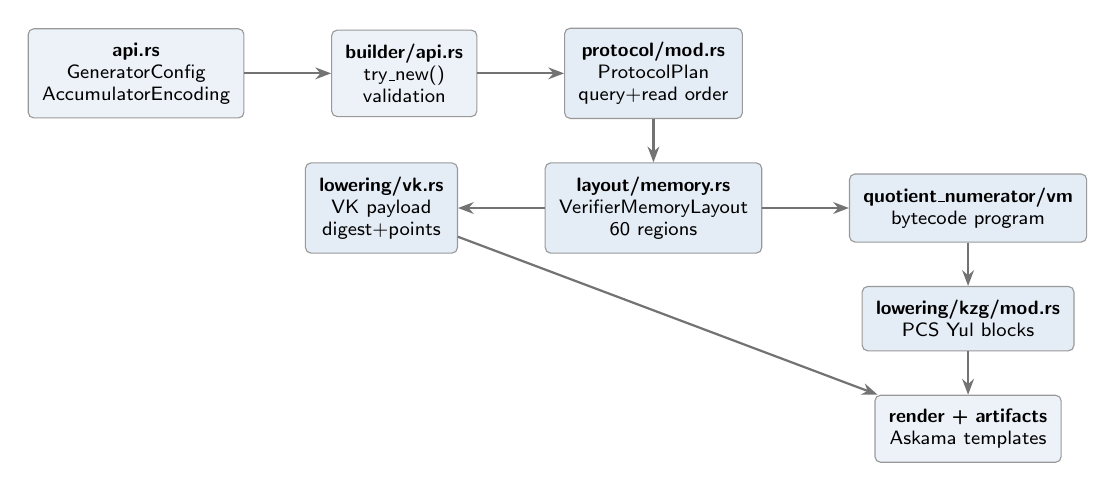
\begin{tikzpicture}[
  node distance=0.55cm and 1.1cm,
  box/.style={draw=black!40, rounded corners=2pt, align=center,
              inner sep=5pt, font=\scriptsize\sffamily},
  arr/.style={-{Stealth[length=2mm]}, black!55, thick}]
\node[box, fill=codegenblue!8] (api) {\textbf{api.rs}\\GeneratorConfig\\AccumulatorEncoding};
\node[box, fill=codegenblue!8, right=of api] (inputs) {\textbf{builder/api.rs}\\try\_new()\\validation};
\node[box, fill=codegenblue!12, right=of inputs] (proto) {\textbf{protocol/mod.rs}\\ProtocolPlan\\query+read order};
\node[box, fill=codegenblue!12, below=of proto] (mem) {\textbf{layout/memory.rs}\\VerifierMemoryLayout\\60 regions};
\node[box, fill=codegenblue!12, left=of mem] (vk) {\textbf{lowering/vk.rs}\\VK payload\\digest+points};
\node[box, fill=codegenblue!12, right=of mem] (quot) {\textbf{quotient\_numerator/vm}\\bytecode program};
\node[box, fill=codegenblue!12, below=of quot] (kzgp) {\textbf{lowering/kzg/mod.rs}\\PCS Yul blocks};
\node[box, fill=codegenblue!8, below=of kzgp] (render) {\textbf{render + artifacts}\\Askama templates};
\draw[arr] (api) -- (inputs);
\draw[arr] (inputs) -- (proto);
\draw[arr] (proto) -- (mem);
\draw[arr] (mem) -- (vk);
\draw[arr] (mem) -- (quot);
\draw[arr] (quot) -- (kzgp);
\draw[arr] (vk) -- (render);
\draw[arr] (kzgp) -- (render);
\end{tikzpicture}
\end{center}

The entry point is \cg{SolidityGenerator} (\cg{builder/mod.rs}):
\begin{lstlisting}[style=rust]
pub struct SolidityGenerator { params, vk, num_instances, acc_encoding, meta }
impl SolidityGenerator {
    fn inputs(&self) -> VerifierBuildInputs { ... }
    pub fn render(&self, options: RenderOptions) -> RenderedArtifacts { ... }
}
\end{lstlisting}
\cg{RenderOptions} selects which artifacts to emit: the verifier contract,
optionally a separate VK contract, and optionally an external quotient
evaluator contract (Section~\ref{sec:quotient-render}).

\section{Validation: what the generator refuses}
\label{sec:validation}

\cg{builder/\allowbreak{}api.rs::try\_\allowbreak{}new} runs the profile checks of
Section~\ref{sec:profile} before any planning:
\begin{itemize}[leftmargin=1.4em,itemsep=1pt]
  \item \cg{NoAdviceColumns} --- a circuit with no advice cannot be verified.
  \item \cg{validate\_\allowbreak{}instance\_\allowbreak{}column\_\allowbreak{}shape} --- exactly one committed
        instance column (the identity commitment) and exactly one
        non-committed instance column.
  \item accumulator validation --- if an outer IVC accumulator is present,
        its encoding (offset, 7 limbs of 56 bits, PointAndScalar/PointPair)
        must be consistent.
  \item \cg{RotatedInstanceQuery} rejection --- non-committed instance
        columns may only be queried at rotation~0.
\end{itemize}
These mirror the Rust verifier's own instance validation
(\rust{verifier.rs} L263--268) but are \emph{stricter}: the Rust verifier
would accept shapes the generator deliberately excludes. This asymmetry is
safe --- the generator only claims faithfulness inside its profile.

\section{The protocol plan}
\label{sec:protocol-plan}

\cg{lowering/\allowbreak{}protocol/\allowbreak{}mod.rs::ProtocolPlan::from\_\allowbreak{}constraint\_\allowbreak{}system}
(1223 L) is the heart of the lowering. It computes, from the constraint
system alone, the exact order of every proof read and every PCS query. The
key data types:

\begin{lstlisting}[style=rust]
enum CommitmentRead { Advice, LookupMultiplicity, PermutationProduct,
                     LookupHelper, LookupAccumulator, Trash, Quotient }
enum PermutationZEval { Cur, Next, Last }
struct Query { rotation: Rotation, comm: ..., eval: ... }
\end{lstlisting}

\paragraph{Proof commitment order} (mirrors \rust{parse\_trace}):\\[2pt]
{\centering\small advices per phase $\rightarrow$ multiplicities $\rightarrow$
perm products $\rightarrow$ helpers+accumulators $\rightarrow$ trash
$\rightarrow$ quotient limbs.\par}

\paragraph{Proof eval order} (mirrors the eval-absorption loop):\\[2pt]
{\centering\small committed\_instance $\rightarrow$ advice $\rightarrow$
fixed (non-simple) $\rightarrow$ perm\_common $\rightarrow$
perm z cur/next/last per set $\rightarrow$
lookup m/helper/z(0)/z(1) $\rightarrow$ trash.\par}

\paragraph{PCS query order} (mirrors \rust{verifier.rs} L577--652):\\[2pt]
{\centering\small advice $\rightarrow$ committed instance $\rightarrow$
perm z $\rightarrow$ lookup $\rightarrow$ trash $\rightarrow$
fixed non-simple $\rightarrow$ perm common $\rightarrow$ linearization.\par}

\subsection{The canonical read-order construction}
\label{sec:read-order}

The ordering above is not hand-written --- it is \emph{derived} from the
constraint system by the plan builder, so the generated proof layout
cannot drift from the circuit. The commitment stream:
\begin{lstlisting}[style=rust]
proof.commitments.extend((0..advice_indices.len())
    .map(|_| CommitmentRead::Advice));                 // per phase
proof.commitments.extend((0..num_lookups)
    .map(|_| CommitmentRead::LookupMultiplicity));
proof.commitments.extend((0..num_permutation_zs)
    .map(|_| CommitmentRead::PermutationProduct));
for &chunks in &lookup_chunks {
    proof.commitments.extend((0..chunks)
        .map(|_| CommitmentRead::LookupHelper));
    proof.commitments.push(CommitmentRead::LookupAccumulator);
}
proof.commitments.extend((0..num_trashcans)
    .map(|_| CommitmentRead::Trash));
proof.commitments.extend((0..num_quotients)
    .map(|_| CommitmentRead::Quotient));
\end{lstlisting}
and the eval stream (note the two deliberate exclusions):
\begin{lstlisting}[style=rust]
proof.evals.extend(instance_queries.iter().copied()
    .filter(|q| q.column < nb_committed_instances)   // committed only
    .map(EvalRead::CommittedInstance));
proof.evals.extend(advice_queries.iter().copied().map(EvalRead::Advice));
proof.evals.extend(fixed_queries.iter().copied()
    .filter(|q| !simple_selector_cols.contains(&q.column))  // no simple sel.
    .map(EvalRead::Fixed));
// perm common, then per-set z cur/next/last (last skipped on final set)
for set in 0..num_permutation_zs {
    proof.evals.push(EvalRead::PermutationZ { set, kind: Cur });
    proof.evals.push(EvalRead::PermutationZ { set, kind: Next });
    if set + 1 != num_permutation_zs {
        proof.evals.push(EvalRead::PermutationZ { set, kind: Last });
    }
}
// lookup m / helper / z(0) / z(1), then trash
\end{lstlisting}
\begin{itemize}
  \item \textcolor{tracegreen}{\textbf{[OK] Derived, not hand-written.}}
        The order is computed from \rust{cs.advice\_\allowbreak{}queries()} etc., so
        adding a column to the circuit automatically shifts the proof
        layout --- the generated parser and the Rust verifier stay in
        lockstep by construction.
  \item \textcolor{tracegreen}{\textbf{[OK] Simple-selector exclusion.}}
        Simple selector columns are filtered out of the eval stream
        (filled by the linearization path, not read from the proof),
        matching the Rust verifier's treatment.
  \item \textcolor{tracegreen}{\textbf{[OK] Final-set \texttt{Last}
        skip.}} The \texttt{Last} rotation is omitted on the final
        permutation set --- the same boundary condition the Rust
        permutation verifier applies (the last set's last-row term is
        folded elsewhere).
  \item \textcolor{mathpurple}{\textbf{[NOTE] Phase remapping.}} The
        \cg{remapping} closure repacks declaration-order advice/challenge
        columns into phase-packed order (\cg{nums}/\cg{index}), because
        Midnight declares columns in source order but verifies them phase
        by phase. This is the one place where the wire order differs from
        the declaration order; the generated parser must use the
        remapped indices.
\end{itemize}

\subsection{Lookup chunking: \cg{nb\_\allowbreak{}parallel\_\allowbreak{}lookups\_\allowbreak{}per\_\allowbreak{}chunk}}
\label{sec:lookup-chunking}

The \cg{lookup\_chunks} field (which sizes the helper commitments and
evals in the proof layout) is derived from the LogUp degree budget:
\begin{lstlisting}[style=rust]
pub(crate) fn nb_parallel_lookups_per_chunk(&self, cs_degree: usize) -> usize {
    let max_degree = (cs_degree - 1).next_power_of_two() + 1;
    let lookup_degree = self.input_expressions.iter()
        .flat_map(|e| e.iter().map(|e| e.degree()))
        .max().unwrap_or(1);
    // dominating factor: h(X) * prod_j (f_j(X) + beta)
    //   has degree 1 + lookup_degree * nb_parallel_lookups
    (max_degree - 1) / lookup_degree
}
\end{lstlisting}
\begin{itemize}
  \item \textcolor{tracegreen}{\textbf{[OK] Degree-budget derivation.}}
        The chunk size is the largest number of parallel LogUp inputs
        whose dominating polynomial $h(X)\prod_j(f_j(X)+\beta)$ fits the
        constraint-system degree budget. \cg{chunk\_by\_degree} then
        splits \texttt{input\_\allowbreak{}expressions} into that many per chunk,
        each becoming one committed helper $h_i(X)$.
  \item \textcolor{tracegreen}{\textbf{[OK] Verifier-side consistency.}}
        The generated verifier reads exactly \cg{num\_chunks} helper
        commitments and their evals per lookup (the
        \texttt{LookupHelper}/\texttt{LookupAccumulator} reads in
        \S\ref{sec:read-order}), so the chunking formula is the single
        source of truth for the lookup portion of the proof layout.
  \item \textcolor{mathpurple}{\textbf{[NOTE] \texttt{next\_\allowbreak{}power\_\allowbreak{}of\_\allowbreak{}two}
        rounding.}} \texttt{max\_degree} rounds \texttt{cs\_degree-1}
        up to a power of two before adding 1, matching the Rust
        verifier's degree handling. A circuit whose degree is not a
        power of two gets a slightly larger budget --- faithful to
        Rust, but worth noting when reasoning about chunk counts.
\end{itemize}

The plan's \cg{validate()} method asserts internal invariants: every
commitment read is consumed by at least one PCS query (so the
no-curve-check-at-absorption argument of Definition~\ref{def:g1-canonical}
holds --- every absorbed point is later validated by a precompile), and the
eval counts match \cg{ConstraintSystemMeta::num\_\allowbreak{}evals}.

\begin{claim}[Query-order faithfulness]
The \cg{ProtocolPlan} query order is identical to the order in which
\rust{verify\_\allowbreak{}algebraic\_\allowbreak{}constraints} builds its \rust{queries} vector.
This is verified by the differential trace: the PCS point-set trace ids
\boxid{41000+s} and q\_com ids \boxid{40000+s} must match between Rust
and Solidity, which pins both the set partition and the within-set order.
\end{claim}

\section{Memory layout}
\label{sec:memlayout}

\cg{layout/\allowbreak{}memory.rs::VerifierMemoryLayout} (1468 L) assigns ~60 named
regions with a bump allocator and a \cg{MemoryMap.validate} pass. The
regions (poseidon fixture addresses) are:

\begin{longtable}{@{}llp{0.42\linewidth}@{}}
\toprule
\textbf{Region} & \textbf{Addr} & \textbf{Purpose} \\
\midrule
\endfirsthead
\toprule
\textbf{Region} & \textbf{Addr} & \textbf{Purpose} \\
\midrule
\endhead
\texttt{transcript\_mptr} & 0x1000 & Keccak buffer (Def.~\ref{def:squeeze}). \\
\texttt{vk\_mptr} & 0x1980 & VK payload (digest, k, $\omega$, points). \\
\texttt{challenge\_mptr} & 0x2b60 & base of challenge block. \\
\texttt{theta/beta/gamma} & 0x2b60/80/a0 & randomizers. \\
\texttt{trash\_\allowbreak{}challenge/\allowbreak{}y/\allowbreak{}x} & 0x2bc0/e0/00 & batching challenges. \\
\texttt{x1/x2/x3/x4} & 0x2c20--0x2c80 & multi-open challenges. \\
\texttt{f\_com / pi} & 0x2ca0 / 0x2d20 & PCS commitments. \\
\texttt{x\_\allowbreak{}n, x\_\allowbreak{}n\_\allowbreak{}minus\_\allowbreak{}1\_\allowbreak{}inv} & 0x2ea0/0x2ec0 & $x^n$, $(x^n-1)^{-1}$. \\
\texttt{l\_\allowbreak{}last/\allowbreak{}l\_\allowbreak{}blind/\allowbreak{}l\_\allowbreak{}0} & 0x2ee0/f0/2f20 & Lagrange specials. \\
\texttt{instance\_eval} & 0x2f40 & Eq.~\eqref{eq:instance-eval}. \\
\texttt{quotient\_eval} & 0x2f60 & $-\nu_y(x)$ (Def.~\ref{def:neg-numer}). \\
\texttt{quotient} & 0x2f80 & $x_{\mathsf{split}}$, $1-x^n$ (2 words). \\
\texttt{f\_\allowbreak{}eval /\allowbreak{} v /\allowbreak{} final\_\allowbreak{}com} & 0x3020/40/60 & Eqs.~\eqref{eq:feval},\eqref{eq:v}. \\
\texttt{pairing\_lhs/rhs} & 0x30e0/0x3160 & pairing inputs. \\
\texttt{rot\_points} & 0x31e0 & $x\cdot\omega^{\text{rot}}$ table. \\
\texttt{x1\_powers} & 0x3560 & truncated $x_1^i$. \\
\texttt{q\_\allowbreak{}com /\allowbreak{} q\_\allowbreak{}eval\_\allowbreak{}set} & 0x3d80 & per-set batched comms/evals. \\
\texttt{g1\_identity} & 0x4580 & 128 zero bytes. \\
\texttt{reversed\_evals} & 0x46e0 & eval spill for VM. \\
\texttt{comms bases} & 0x4ce0+ & per-category commitment regions. \\
\texttt{selector\_acc} & 0x5660 & simple-selector buckets $B_j$. \\
\texttt{quotient\_\allowbreak{}tmp/\allowbreak{}stack} & 0x56e0+ & VM scratch. \\
\bottomrule
\end{longtable}

The layout is computed \emph{before} rendering so that templates receive
final addresses; \cg{plan.rs} checks for \cg{eval\_\allowbreak{}numer\_\allowbreak{}mptr drift}
between planning and rendering passes.

\section{VK payload}
\label{sec:vkpayload}

\cg{lowering/\allowbreak{}vk.rs::generate\_\allowbreak{}base\_\allowbreak{}vk} (448 L) produces the VK payload
consumed by \sol{VkLoading.yul}:
\begin{itemize}[leftmargin=1.4em,itemsep=1pt]
  \item \cg{vk\_digest} $= \texttt{fe\_to\_u256}(\texttt{vk.transcript\_\allowbreak{}repr()})$
        --- Eq.~\eqref{eq:vk-digest}.
  \item \texttt{k}, \texttt{n\_inv}, \texttt{omega}, \texttt{omega\_inv},
        \texttt{omega\_inv\_to\_l} $= \omega_{\mathsf{inv}}^{|\text{rotation\_last}|}$.
  \item accumulator metadata (offset, limb count, limb bits).
  \item base points: \texttt{G1Base} $=G$, \texttt{G2Base} $=G_2$,
        \texttt{NegSG2Base} $-[s]_2$, encoded via \cg{g1\_to\_u256s}/
        \cg{g2\_to\_u256s}.
\end{itemize}
The \cg{TranscriptBufferLayout} sizes the transcript buffer at 128 bytes
per G1 (a comment records a historical 49-byte bug that broke digest
binding --- the fix is pinned by tests).

\section{Proof layout and repacking}
\label{sec:prooflayout}

\cg{lowering/\allowbreak{}abi/\allowbreak{}proof.rs::ProofCalldataLayout} (537 L) defines the
compressed proof byte layout: advice phases, lookup multiplicities,
permutation products, lookups, trash, quotient limbs, evals, f\_com,
q\_evals, pi, with byte cursors. \cg{lowering/\allowbreak{}calldata.rs::repack\_\allowbreak{}proof}
(144 L) converts a native proof to the on-chain form:
\begin{itemize}[leftmargin=1.4em,itemsep=1pt]
  \item each 48-byte compressed G1 $\rightarrow$ 128-byte EIP-2537
        uncompressed (16 zero pad $+\, x_{\mathsf{hi}}/x_{\mathsf{lo}} + 16$
        zero pad $+\, y_{\mathsf{hi}}/y_{\mathsf{lo}}$); identity $\rightarrow$
        128 zeros.
  \item scalars little-endian $\rightarrow$ big-endian words.
\end{itemize}
The walk is driven by \cg{RepackedProofLayoutPlan} so the repacker and the
generated parser cannot drift apart.

\section{The quotient virtual machine}
\label{sec:quotient-vm}

The expensive part of the verifier is reconstructing $\nu_y(x)$ from the
identity expressions. Rather than emitting straight-line Yul for every
gate (which explodes code size), the generator compiles the identities
into a compact \textbf{bytecode program} executed by a small VM embedded
in the contract (\cg{quotient\_\allowbreak{}numerator/\allowbreak{}vm/\allowbreak{}mod.rs}, 3852 L).

\paragraph{Opcodes} (Q\_OP\_*, 31 opcodes in 0x01--0x22;
\cg{vm/mod.rs} L560--590; 0x17, 0x18, 0x1a unassigned):
\begin{lstlisting}[style=plain]
0x01 push_const         0x09 push_const_u8      0x13 add_mul_const_u8_mem_u16
0x02 push_mem_literal   0x0a fold_main          0x14 add_mul_mem_mem
0x03 push_mem_token     0x0b fold_selector      0x15 run of 0x12
0x04 push_mem_token_off 0x0c add_const_u8       0x16 run of 0x13
0x05 push_mem_u16       0x0d mul_const_u8       0x19 native_permutation
0x06 add                0x0e add_const          0x1b native_identity
0x07 mul                0x0f mul_const          0x1c LIN7   0x1d BILIN7_ROW
0x08 neg                0x10 add_mem_u16        0x1e BILIN7_PAIRWISE
                        0x11 mul_mem_u16        0x1f native_lookup  0x20 POW5
                        0x12 add_mul_mem_mem_const_u8   0x21 MODARITH7  0x22 AFFINE_SUM
\end{lstlisting}
The rendered dispatch loop is pruned to the opcodes the program actually
uses (\cg{quotient\_\allowbreak{}program\_\allowbreak{}usage}); an opcode that is not rendered falls
into the \texttt{default} revert. The production B64 program uses 11 of
the 31 (\S\ref{sec:pr-isa-dispatch}).
\paragraph{Memory tokens} (Q\_MEM\_*, 0x01--0x09):
\texttt{L0, L\_\allowbreak{}LAST, L\_\allowbreak{}BLIND, BETA, GAMMA, X, THETA, TRASH\_\allowbreak{}CHALLENGE,
INSTANCE\_\allowbreak{}EVAL}.

The VM registers are \texttt{q\_\allowbreak{}pc, q\_\allowbreak{}end, q\_\allowbreak{}sp, q\_\allowbreak{}top, q\_\allowbreak{}has\_\allowbreak{}top}
(a one-element top-of-stack cache). \cg{QuotientProgramBuilder} folds
each identity with the Horner $y$-weighting of \eqref{eq:nu-y}:
\cg{fold\_identity} emits \texttt{fold\_main} (into the main numerator)
or \texttt{fold\_\allowbreak{}selector(idx)} (into bucket $B_j$). The final VM
instruction sequence ends with
\begin{lstlisting}[style=yul]
// linearization_expected_eval = -quotient_eval_numer
mstore(QUOTIENT_EVAL_MPTR, sub(r, quotient_eval_numer))
\end{lstlisting}
which is Definition~\ref{def:neg-numer} / Eq.~\eqref{eq:expected-eval}.

\paragraph{Native fast paths.} Common expression shapes are compiled to
fused opcodes rather than generic push/add/mul sequences:
\texttt{LIN7} (linear combination of 7 terms), \texttt{BILIN7\_ROW}
(bilinear 7-term), \texttt{MODARITH7}, \texttt{POW5}, and the
\texttt{native\_\allowbreak{}permutation}/\texttt{native\_lookup}/\texttt{native\_identity}
callbacks that jump into hand-written Yul blocks for the permutation and
lookup identity families. The \cg{QuotientProgramPlan} classifies each
identity into \cg{inline\_\allowbreak{}identities}, \cg{native\_\allowbreak{}identities},
\cg{native\_\allowbreak{}permutation\_\allowbreak{}identities}, \cg{native\_\allowbreak{}lookup\_\allowbreak{}identities}.

\paragraph{Limb arithmetic.} Foreign-field (BLS12-381 base field) gadgets
constrain values held as 7 limbs of 56 bits. The VM does not perform wide
arithmetic: every operation is a native $\Fr$ \texttt{addmod}/\texttt{mulmod}.
The limb helpers \cg{q\_limb7}/\cg{q\_limb7\_wide} in
\sol{QuotientHelpers.yul} evaluate the fixed linear forms
$\sum_i c_i\,\ell_i \bmod r$ with the base-power coefficients
\cg{LIMB7\_\allowbreak{}YUL\_\allowbreak{}COEFFS}/\cg{WIDE\_\allowbreak{}LIMB7\_\allowbreak{}YUL\_\allowbreak{}COEFFS}, and \cg{q\_pow5}
evaluates the Poseidon S-box term $x^5$. Each helper is rendered only when
the lowering recognizes the matching expression shape.

\section{PCS lowering}
\label{sec:pcs-codegen}

\cg{lowering/\allowbreak{}kzg/\allowbreak{}mod.rs} (2077 L) emits the Yul blocks that implement
Eqs.~\eqref{eq:qcom}--\eqref{eq:finalcom}. Its \cg{computations()}
method produces:
\begin{enumerate}[leftmargin=1.4em,itemsep=1pt]
  \item \textbf{Rotation points}: $x\cdot\omega^{\text{rot}}$ written to
        \texttt{ROT\_POINTS\_MPTR} (mirrors \rust{rotate\_omega}).
  \item \textbf{$x_1$ powers}: truncated $x_1^i$ to
        \texttt{X1\_POWERS\_MPTR} (Eq.~\eqref{eq:qcom} scalars).
  \item \textbf{q\_eval\_set folds}: per-set $\sum_k x_1^k v_{s,k}$
        (Eq.~\eqref{eq:qeval}), with a roll threshold
        \cg{Q\_\allowbreak{}EVAL\_\allowbreak{}ROLL\_\allowbreak{}THRESHOLD=4} for register pressure.
  \item \textbf{q\_com} (trace-only): the per-set batched commitment.
  \item \textbf{Fused final MSM}: the linearization expansion ---
        quotient limbs $\times\,(1-x^n)\cdot x_{\mathsf{split}}^i$
        $\times$ query scalar, plus selector buckets $\times$ fixed
        commitments --- as one G1MSM (Eq.~\eqref{eq:linearization}
        commitment side).
  \item \textbf{v computation}: $v = \sum_s x_4^s q_{\mathsf{eval}}^{(s)}
        + x_4^{n_{\text{sets}}} f_{\mathsf{eval}}$ (Eq.~\eqref{eq:v}).
  \item \textbf{Final pairing inputs}.
\end{enumerate}
\cg{validate\_\allowbreak{}g1\_\allowbreak{}precompile\_\allowbreak{}coverage} asserts every absorbed G1 point
appears in a G1MSM or pairing input --- the formal counterpart of
Definition~\ref{def:g1-canonical}'s ``validated by precompile'' claim.

\subsection{\cg{construct\_\allowbreak{}intermediate\_\allowbreak{}sets\_\allowbreak{}impl} --- the point-set partition}
\label{sec:construct-sets}

This is the codegen core of the KZG multi-open (Sec.~\ref{sec:pointsets}).
It mirrors the Rust \rust{construct\_\allowbreak{}intermediate\_\allowbreak{}sets} but is
deterministic and side-effect-free so the generated schedule is auditable:
\begin{lstlisting}[style=rust]
fn construct_intermediate_sets_impl(queries: &[Query]) -> IntermediateSets {
    // Step 1: one entry per unique commitment; one index per unique rotation.
    let mut commitment_map: Vec<(EcPoint, Vec<usize>, Vec<Word>)> = Vec::new();
    let mut point_index_of: Vec<i32> = Vec::new();
    for query in queries {
        let point_idx = /* intern query.rotation */;
        if let Some(slot) = commitment_map.find(|c| *c == query.comm) {
            if let Some(pos) = slot.1.position(|pi| *pi == point_idx) {
                // Same (comm, rotation) twice: evals MUST agree, else the
                // proof claims one poly opens to two values -> reject.
                assert_eq!(slot.2[pos], query.eval,
                    "duplicate (commitment, rotation) query with conflicting evals");
                continue;
            }
            slot.1.push(point_idx); slot.2.push(query.eval);
        } else {
            commitment_map.push((query.comm, vec![point_idx], vec![query.eval]));
        }
    }
    // Step 2: bucket by sorted point-index set (BTreeMap => deterministic).
    let mut point_idx_sets: BTreeMap<Vec<usize>, usize> = BTreeMap::new();
    for (_, point_indices, _) in &commitment_map {
        let mut sorted = point_indices.clone(); sorted.sort_unstable(); sorted.dedup();
        let n = point_idx_sets.len();
        point_idx_sets.entry(sorted).or_insert(n);   // capture INSERTION order
    }
    // Step 3: align each commitment's evals to the sorted point order.
    // Step 4: point_sets[set_idx] = rotations (set_idx = insertion order).
    ...
}
\end{lstlisting}
\begin{itemize}
  \item \textcolor{tracegreen}{\textbf{[OK] Conflict rejection.}} A
        duplicate $(\text{comm},\text{rotation})$ with \emph{different}
        evals is a protocol bug and is asserted against --- the codegen
        refuses to emit a schedule for an inconsistent query set.
  \item \textcolor{tracegreen}{\textbf{[OK] Deterministic insertion-order
        capture.}} The comment warns that the \texttt{or\_insert(n)}
        insertion order (not the BTreeMap iteration order) is the
        set-index used downstream and as the \texttt{sort\_sets}
        tiebreak. This is the same ordering the Rust verifier relies on
        so the first point set holds the fixed commitments opened at
        $x$ (Sec.~\ref{sec:pcs-math}).
  \item \textcolor{mathpurple}{\textbf{[NOTE] \texttt{HashMap} hazard.}}
        The comment explicitly flags that swapping the \texttt{BTreeMap}
        for a \texttt{HashMap} would break the insertion-order capture.
        This is a latent maintenance trap; the invariant is documented
        but not type-enforced.
\end{itemize}

\subsection{\cg{sort\_sets} --- ascending-cardinality ordering}
\label{sec:sort-sets}

After the partition, the sets are sorted so the generated schedule is
deterministic and the first set holds the fixed commitments opened at
$x$ only:
\begin{lstlisting}[style=rust]
fn sort_sets(input: IntermediateSets) -> IntermediateSets {
    let mut order: Vec<usize> = (0..input.point_sets.len()).collect();
    order.sort_by_key(|&i| (input.point_sets[i].len(), i));  // (|S|, idx)
    // remap[old_idx] = new_idx
    let mut remap = vec![0usize; input.point_sets.len()];
    for (new_idx, &old_idx) in order.iter().enumerate() {
        remap[old_idx] = new_idx;
    }
    let point_sets = order.iter().map(|&i| input.point_sets[i].clone()).collect();
    let commitments = input.commitments.into_iter().map(|mut c| {
        c.set_index = remap[c.set_index]; c
    }).collect();
    IntermediateSets { commitments, point_sets }
}
\end{lstlisting}
\begin{itemize}
  \item \textcolor{tracegreen}{\textbf{[OK] \texttt{(|S|, idx)} tiebreak.}}
        Sorting by ascending cardinality then original index matches the
        Rust \rust{sort\_\allowbreak{}by\_\allowbreak{}key($\vert i\vert$, i)} (Sec.~\ref{sec:pointsets}),
        so the within-set eval order and the $x_1$-power assignment are
        identical between Rust and the generated verifier.
  \item \textcolor{tracegreen}{\textbf{[OK] \texttt{set\_index} rewrite.}}
        Every commitment's \texttt{set\_index} is remapped through the
        same permutation, so downstream \cg{commitments\_\allowbreak{}by\_\allowbreak{}set} and the
        fused-MSM grouping see the sorted order consistently.
\end{itemize}

\subsection{\cg{used\_lagrange} --- required common polynomials}
\label{sec:used-lagrange}

The plan also records which Lagrange polynomials the verifier must
materialize, so the generated \texttt{Lagrange.yul} block computes
exactly what is needed:
\begin{lstlisting}[style=rust]
pub(crate) fn used_lagrange(
    uses_permutation: bool, uses_lookup: bool, uses_trash: bool,
) -> BTreeSet<CommonPoly> {
    let mut out = BTreeSet::new();
    if uses_permutation || uses_lookup {
        out.insert(CommonPoly::L0);
        out.insert(CommonPoly::LLast);
        out.insert(CommonPoly::LBlind);
    }
    if uses_trash {
        out.insert(CommonPoly::Rotation(0));
    }
    out
}
\end{lstlisting}
\begin{itemize}
  \item \textcolor{tracegreen}{\textbf{[OK] Minimal materialization.}}
        $l_0, l_{\text{last}}, l_{\text{blind}}$ are computed only when
        a permutation or lookup argument is present; the trash argument
        additionally needs the rotation-0 Lagrange. A circuit with no
        perm/lookup/trash computes none of them --- a real gas saving
        over always computing the full Lagrange basis.
  \item \textcolor{mathpurple}{\textbf{[NOTE] \texttt{CommonPoly} enum.}}
        The \texttt{Rotation(i)} variant generalizes to arbitrary
        rotations, though in the current verifier only rotation 0 is
        requested by trash. The generated code handles the general case
        but only the specific requests appear in practice.
\end{itemize}

\subsection{\cg{computations()} --- the Yul emitter}
\label{sec:computations}

\cg{computations()} is the function that actually emits the PCS Yul
blocks (the \texttt{pcs\_computations} consumed by
\texttt{Pcs.yul}). It mirrors the Rust \rust{multi\_prepare} flow as a
sequence of emitted blocks. Block 1 pre-computes the rotation points
$x\cdot\omega^{\text{rot}}$ by walking forward/backward from rotation 0:
\begin{lstlisting}[style=rust]
// Block 1: rotation points x*omega^rot at ROT_POINTS_MPTR + 32*idx
let x_pow_of_omega := x;                       // rot 0 = x
for rot in 1..=max_rot {
    x_pow_of_omega := mulmod(x_pow_of_omega, omega, r);
    store_rot(rot);                            // if rot is used
}
if min_rot < 0 {
    x_pow_of_omega := x;
    for rot in (min_rot..0).rev() {
        x_pow_of_omega := mulmod(x_pow_of_omega, omega_inv, r);
        store_rot(rot);
    }
}
\end{lstlisting}
Block 2 pre-computes the $x_1$ powers, with a deliberate
\textbf{rolled-loop} optimization:
\begin{lstlisting}[style=rust]
// Block 2: x1^0..x1^(nb-1) at X1_POWERS_MPTR
let acc := 1
let p := X1_POWERS_MPTR
for { let i := 0 } lt(i, {last}) { i := add(i, 1) } {
    p := add(p, 32)
    acc := mulmod(acc, x1, r)
    mstore(p, and(acc, TRUNC_MASK_128))   // if truncated_challenges
}
\end{lstlisting}
\begin{itemize}
  \item \textcolor{codegenblue}{\textbf{[IMPROVE] Rolled vs.\ unrolled
        (already applied).}} The codegen comment records that the
        \emph{unrolled} emission (32 sequential \texttt{mulmod}+
        \texttt{mstore} pairs) cost $\sim$26\,kg of gas --- far above
        the $\sim$700 gas the arithmetic needs --- because
        \texttt{solc --ir} cannot register-allocate 32 unrolled
        \texttt{mulmods} sharing one accumulator, and the unrolled
        \texttt{mstore}-\texttt{add} chain inflates each line to
        $\sim$50--60 gas of dispatch overhead. The rolled loop restores
        the basic-block heuristic ($\sim$20 gas/iter $\times$ 32 + 50
        setup $\approx$ 700 gas). This is a concrete, measured
        contract-space/gas win baked into the generator.
  \item \textcolor{tracegreen}{\textbf{[OK] Truncated-challenge mask.}}
        When \texttt{truncated\_\allowbreak{}challenges} is set, the emitted loop
        stores \texttt{and(acc, mask)} while keeping \texttt{acc} at
        full precision --- exactly mirroring the Rust
        \rust{powers(x1).map(truncate)} (full-precision running
        accumulator, truncated per element). The \texttt{+3} gas/iter
        for the mask is negligible vs the loop body.
  \item \textcolor{mathpurple}{\textbf{[NOTE] Trace-scratch borrowing.}}
        In trace mode, Block 1 borrows \texttt{Q\_\allowbreak{}EVAL\_\allowbreak{}SET\_\allowbreak{}MPTR} as
        scratch for the serialized point-set payload, relying on Block 3
        to unconditionally overwrite it before any later read. The
        comment flags that a future reader between Block 1 and Block 3
        must move the scratch --- a latent coupling to watch.
\end{itemize}

\subsection{\cg{validate\_\allowbreak{}g1\_\allowbreak{}precompile\_\allowbreak{}coverage} --- the safety invariant}
\label{sec:coverage-invariant}

The invariant that makes ``no curve check at absorption'' sound
(cf.\ \S\ref{sec:common-g1}):
\begin{lstlisting}[style=rust]
fn validate_g1_precompile_coverage(
    absorbed: &[TrackedG1], precompile_inputs: &[TrackedG1],
) -> Result<(), String> {
    let missing: Vec<&TrackedG1> = absorbed.iter()
        .filter(|a| !precompile_inputs.iter().any(|c| c.point == a.point))
        .collect();
    if let Some(first) = missing.first() {
        return Err(format!("{} absorbed proof G1(s) are not consumed by a later \
            EIP-2537 G1MSM/pairing precompile; first missing: {} at {}",
            missing.len(), first.label, first.point.ptr()));
    }
    Ok(())
}
\end{lstlisting}
The wrapper
\cg{validate\_\allowbreak{}absorbed\_\allowbreak{}g1\_\allowbreak{}precompile\_\allowbreak{}coverage} first checks the
absorbed count equals the proof layout's \texttt{total\_\allowbreak{}g1\_\allowbreak{}count()}
(so no absorbed point is untracked), then runs the coverage check
against \cg{precompile\_\allowbreak{}validated\_\allowbreak{}g1s}.

\begin{itemize}
  \item \textcolor{tracegreen}{\textbf{[OK] Concrete-handle checking.}}
        The check operates on the \emph{emitted memory handles}
        (\texttt{TrackedG1.point.ptr()}), not just the logical PCS
        queries --- so it catches quotient limbs hidden behind the
        synthetic linearization commitment.
  \item \textcolor{rustorange}{\textbf{[RISK] Point-equality by pointer.}}
        Coverage is decided by \texttt{candidate.point == absorbed.point}
        (memory-handle equality). If the same logical point is materialized
        at two different addresses (e.g.\ a copy), the absorbed handle
        would be reported as ``not covered'' even though an equal point
        is MSM'd. This is conservative (fails closed, build error), but
        could cause a false build failure if the codegen ever duplicates
        a point's storage. \emph{Audit note:} the codegen must keep one
        canonical address per absorbed point.
\end{itemize}

\section{Rendering}
\label{sec:render}

\cg{lowering/\allowbreak{}artifacts.rs::generate\_\allowbreak{}verifier\_\allowbreak{}from\_\allowbreak{}plan} assembles the
Askama model (verifier template + included partials) and renders the
Solidity source; \cg{validate\_layout} panics on any invalid plan so a
broken lowering never produces a contract. \cg{render/models.rs} holds the
template data models. The \cg{QuotientRendering} enum
(Section~\ref{sec:quotient-vm}) selects between:
\begin{itemize}[leftmargin=1.4em,itemsep=1pt]
  \item \cg{Compact} --- the VM is inlined in the main verifier.
  \item \cg{External} --- the verifier \texttt{staticcall}s a pinned
        \sol{Halo2QuotientEvaluator} (codehash-checked), passing the raw
        verifier memory frame as calldata.
\end{itemize}

% ============================================================================
% Part 5 --- The generated Solidity / Yul
% ============================================================================
\chapter{The Generated Solidity and Yul}
\label{ch:solidity}

The generated artifact is a single Solidity contract, \sol{Halo2Verifier.sol},
whose entry point is
\begin{lstlisting}[style=yul]
function verifyProof(bytes calldata proof, bytes[] calldata instances)
    external view returns (bool)
\end{lstlisting}
with selector \cg{FN\_\allowbreak{}SIG\_\allowbreak{}VERIFY\_\allowbreak{}PROOF} $=$ \texttt{0x1e8e1e13}. The
function body is one \texttt{assembly ("memory-safe")} block containing
included Yul partials. It is \textbf{terminal}: every failure path is a
\texttt{revert}; the only non-reverting exit is
\texttt{mstore(RETURN\_\allowbreak{}MPTR,1); return(RETURN\_\allowbreak{}MPTR,0x20)}.

\section{Contract structure}
\label{sec:sol-structure}

\begin{lstlisting}[style=plain]
contract Halo2Verifier {
    // Constants.sol: FR_MODULUS, BLS_P_HI/LO, EXPECTED_VK_*, ABI cursors,
    //                VK memory map, challenge layout
    // PrecompileSmoke.sol: MCOPY + G1ADD/G1MSM/PAIRING identity probes
    // Constructors.sol: constructor runs smoke probes + VK pin check
    function verifyProof(...) external view returns (bool) {
        assembly ("memory-safe") {
            // AssemblyHelpers.yul   (scalar_inv, transcript, batch_invert, ec_pairing)
            // AccumulatorHelpers.yul (accumulator decode/validate)
            // TraceAndGasHelpers.yul (trace hooks, gas checkpoints)
            // VkLoading.yul         (embedded or external VK payload load)
            // TranscriptProofParser.yul (the whole proof read + challenge schedule)
            // Lagrange.yul          (x^n, Lagrange basis, instance_eval)
            // QuotientAndLinearization.yul (VM run or external evaluator call)
            // Pcs.yul               (rendered PCS computation blocks)
            // FinalPairing.yul      (accumulator batching + final pairing)
            // TraceReturn.yul       (trace dump + return 1)
        }
    }
}
\end{lstlisting}

\section{ABI and shape guard}
\label{sec:abi}

The generated contract pins the ABI layout with compile-time cursor
constants:
\begin{lstlisting}[style=yul]
uint256 internal constant PROOF_LEN_CPTR    = 0x44;
uint256 internal constant PROOF_CPTR        = 0x64;
uint256 internal constant NUM_INSTANCE_CPTR = 0x1144;
\end{lstlisting}
Before any memory work, a shape guard rejects malformed calls:
\begin{lstlisting}[style=yul]
if iszero(and(eq(calldataload(0x04), 0x40),
              eq(calldataload(0x24), sub(NUM_INSTANCE_CPTR, 0x04)))) { revert(0,0) }
\end{lstlisting}
This checks the dynamic-array offset is \texttt{0x40} and the proof length
matches the generated layout, so a truncated or shifted calldata never
reaches the transcript.

\section{Transcript helpers}
\label{sec:sol-transcript}

The Yul transcript helpers implement Definitions~\ref{def:common}--\ref{def:squeeze}
literally:
\begin{lstlisting}[style=yul]
function common_word(buf_len, word) -> ret {
    mstore(buf_len, word)
    ret := add(buf_len, 32)
}
function squeeze_to(buf_len, mptr) -> ret {
    let h0 := keccak256(TRANSCRIPT_MPTR, sub(buf_len, TRANSCRIPT_MPTR))
    mstore(TRANSCRIPT_MPTR, h0)          // reseed  (eq:transcript-reseed)
    mstore(mptr, mod(h0, r))            // sample  (eq:transcript-squeeze)
    ret := add(TRANSCRIPT_MPTR, 32)
}
\end{lstlisting}
The G1 absorption helper enforces Definition~\ref{def:g1-canonical}:
\begin{lstlisting}[style=yul]
function common_uncompressed_g1(buf_len, cptr) -> ret {
    let x_hi_word := calldataload(cptr)
    let x_lo      := calldataload(add(cptr, 0x20))
    let y_hi_word := calldataload(add(cptr, 0x40))
    let y_lo      := calldataload(add(cptr, 0x60))
    if shr(128, x_hi_word) { revert(0, 0) }   // top 16 bytes must be zero
    if shr(128, y_hi_word) { revert(0, 0) }
    let x_hi := and(x_hi_word, 0xffff...)
    let y_hi := and(y_hi_word, 0xffff...)
    // coordinate < q checks (BLS_P_HI / BLS_P_MINUS_ONE_LO ladder)
    if iszero(or(lt(x_hi, BLS_P_HI),
        and(eq(x_hi, BLS_P_HI), iszero(gt(x_lo, BLS_P_MINUS_ONE_LO))))) { revert(0,0) }
    if iszero(or(lt(y_hi, BLS_P_HI),
        and(eq(y_hi, BLS_P_HI), iszero(gt(y_lo, BLS_P_MINUS_ONE_LO))))) { revert(0,0) }
    calldatacopy(buf_len, cptr, 0x80)   // absorb 128 bytes verbatim
    ret := add(buf_len, 0x80)
}
\end{lstlisting}
The comment in the generated code records that the previous emitter hashed
the 48-byte ZCash compressed encoding with a $384$-bit
$\mathsf{lex}(y) > \mathsf{lex}(p-y)$ sign ladder; switching to the
uncompressed form (matching the patched Rust \rust{to\_\allowbreak{}input}) drops the
ladder entirely.

\section{The proof parser}
\label{sec:sol-parser}

\sol{TranscriptProofParser.yul} walks the proof in the order of
Table~\ref{tab:schedule}. A representative excerpt (advice phase, poseidon
fixture, 8 commitments of 0x80 bytes each):
\begin{lstlisting}[style=yul]
let proof_cptr := PROOF_CPTR
let advice_walk := ADVICE_COMMS_MPTR_BASE
// ---- User phase 1 ----
for { let end := add(proof_cptr, 0x0400) } lt(proof_cptr, end) {} {
    buf_len := common_uncompressed_g1(buf_len, proof_cptr)
    calldatacopy(advice_walk, proof_cptr, 0x80)
    advice_walk := add(advice_walk, 0x80)
    proof_cptr  := add(proof_cptr, 0x80)
}
buf_len := squeeze_to(buf_len, THETA_MPTR)
// multiplicities, beta, gamma, perm z, helpers+acc, trash_challenge,
// trash, y, quotient limbs, x ...
\end{lstlisting}
The eval loop range-checks and spills each scalar:
\begin{lstlisting}[style=yul]
for { let end := add(proof_cptr, 0x0600) } lt(proof_cptr, end) {} {
    let eval := calldataload(proof_cptr)
    if iszero(lt(eval, r)) { revert(0, 0) }   // canonical Fr
    mstore(eval_buf, eval)                    // spill for VM
    buf_len := common_word(buf_len, eval)     // absorb
    proof_cptr := add(proof_cptr, 0x20)
}
\end{lstlisting}
The $x_3$ truncation is applied immediately after squeeze:
\begin{lstlisting}[style=yul]
buf_len := squeeze_to(buf_len, X3_MPTR)
mstore(X3_MPTR, and(mload(X3_MPTR), 0xffffffffffffffffffffffffffffffff))
\end{lstlisting}
and the parser closes with the exact-consumption check:
\begin{lstlisting}[style=yul]
if iszero(eq(proof_cptr, NUM_INSTANCE_CPTR)) { revert(0, 0) }
if iszero(success) { revert(0, 0) }
\end{lstlisting}
The first line proves no section was under- or over-read; the second
collects deferred canonicality failures from public-instance reads.

\section{Lagrange and instance evaluation}
\label{sec:sol-lagrange}

\sol{Lagrange.yul} computes $x^n$ by $k$ repeated squarings
(Eq.~\eqref{eq:zn}), batch-inverts the denominators $(x-\omega^i)$ with
one modexp (EIP-198) via Montgomery's trick, then forms
$L_i = (x^n-1)\cdot n^{-1}\cdot \omega_i / (x-\omega_i)$
(Eq.~\eqref{eq:lagrange}), the blind-row sum \eqref{eq:lblind},
$\ell_0$ \eqref{eq:l0}, and the linear combination
$\widehat{\mathsf{inst}}(x)$ \eqref{eq:instance-eval}.

\section{Quotient and linearization}
\label{sec:quotient-render}

In the \emph{compact} path, \sol{QuotientAndLinearization.yul} runs the
quotient VM (Chapter~\ref{sec:quotient-vm}) inline: the program bytes
live in the VK payload at \texttt{q\_\allowbreak{}const}/\texttt{q\_\allowbreak{}program}; the VM
loop switches on opcodes and folds identities into the main numerator or
selector buckets. It then stores
\begin{lstlisting}[style=yul]
// x_split = x^(n-1), one_minus_x_n at QUOTIENT_MPTR words 0/1
// linearization_expected_eval = -quotient_eval_numer
mstore(QUOTIENT_EVAL_MPTR, sub(r, mload(EVAL_NUMER_MPTR)))
\end{lstlisting}
In the \emph{external} path, the verifier \texttt{staticcall}s the pinned
evaluator (codehash-checked), passing the raw memory frame; the evaluator
returns a compact frame \texttt{[magic, expected\_\allowbreak{}eval, buckets...]} and
the verifier copies the buckets back. The external evaluator's header
comment states the contract explicitly:
\begin{quote}\small
``This contract reconstructs the Rust verifier's y-batched identity
numerator $\nu_y(x)$ and returns the linearization expected scalar
$-\nu_y(x)$. It does not evaluate or trust a quotient scalar $h(x)$. The
quotient limb commitments are handled by Halo2Verifier on the commitment
side as $(1-x^n)\cdot\sum_i x_{\mathsf{split}}^i Q_i$.''
\end{quote}

\section{PCS blocks}
\label{sec:sol-pcs}

\sol{Pcs.yul} renders the \cg{pcs\_\allowbreak{}computations} blocks from
Section~\ref{sec:pcs-codegen}: rotation points, $x_1$ powers, per-set
$q_{\mathsf{eval}}$ folds, the fused final G1MSM for the linearization
commitment, and the $v$ computation. The generated sub-blocks are kept
grouped so gas checkpoints can attribute cost. A representative final-MSM
call:
\begin{lstlisting}[style=yul]
success := staticcall(gas(), 0x0c, 0x56e0, 0x1d60, FINAL_COM_MPTR, 0x80)
success := and(success, eq(returndatasize(), 0x80))
mstore(V_MPTR, v)
\end{lstlisting}
(where \texttt{0x0c} is the G1ADD/G1MSM precompile range per EIP-2537;
the MSM uses \texttt{0x0d}).

\section{Final pairing}
\label{sec:pairing-codegen}

The pairing block assembles the two pairing inputs and calls the helper:
\begin{lstlisting}[style=yul]
// PAIRING_LHS := pi ; PAIRING_RHS := final_com - v*G + x3*pi
mcopy(PAIRING_LHS_MPTR, PI_MPTR, 0x80)
// -v*G via G1ADD with negated scalar, then + final_com, + x3*pi
mcopy(PAIRING_RHS_MPTR, 0x80, 0x80)
...
success := ec_pairing(success, PAIRING_RHS_MPTR, PAIRING_LHS_MPTR)
\end{lstlisting}
The generated comment is explicit about the naming trap:
\begin{quote}\small
``The Yul \texttt{ec\_\allowbreak{}pairing} helper checks $e(\text{arg}_0,[1]_2)\cdot
e(\text{arg}_1,-[s]_2)=1$, i.e.\ $e(\text{arg}_0,[1]_2)=e(\text{arg}_1,[s]_2)$.
The KZG pairing identity is $e(\text{final\_\allowbreak{}com}-vG+x_3\pi,[1]_2) =
e(\pi,[s]_2)$, so arg$_0$ must be the combined RHS and arg$_1$ must be
$\pi$. The \texttt{PAIRING\_\allowbreak{}LHS/RHS} naming follows the dual MSM
accumulator (left $=\pi$, right $=$ combined) and \emph{not} the pairing
argument order. Pass them swapped to \texttt{ec\_\allowbreak{}pairing}.''
\end{quote}
This matches the Rust \rust{DualMSM} \texttt{check}
(\texttt{multi\_\allowbreak{}miller\_\allowbreak{}loop} of $(\mathsf{left}, s\_\allowbreak{}g2)$ and
$(\mathsf{right}, -g_2)$) --- Eq.~\eqref{eq:final-pairing-dual}.

\section{Accumulator batching}
\label{sec:sol-acc}

When an outer IVC accumulator is present, \sol{FinalPairing.yul} derives
$\alpha = \keccak(\text{domain}\,\|\,\text{points})\bmod r$ (zero mapped
to $1$) and checks \eqref{eq:acc-batch} with the accumulator points
batched into the same pairing, so a single pairing precompile call covers
both equations. The accumulator scalars are decoded from the 7-limb
56-bit encoding by \sol{AccumulatorHelpers.yul}
(\texttt{load\_\allowbreak{}acc\_\allowbreak{}coord\_\allowbreak{}shifted}, \texttt{is\_\allowbreak{}bls\_\allowbreak{}p\_\allowbreak{}minus\_\allowbreak{}one},
\texttt{validate\_\allowbreak{}public\_\allowbreak{}accumulator}).

\section{Precompile smoke tests}
\label{sec:sol-smoke}

The constructor runs \sol{PrecompileSmoke.sol}: an MCOPY probe (Cancun+
requirement) and identity-input probes of G1ADD (\texttt{0x0c}), G1MSM
(\texttt{0x0d}), and PAIRING (\texttt{0x0f}). If any precompile is
missing or misbehaves, deployment reverts --- the contract cannot be
deployed on a chain where the verifier would be unsound.

\section{Trace and return}
\label{sec:sol-trace}

Under the trace build, \sol{TraceReturn.yul} emits LOG1 events with the
same trace ids as the Rust verifier (Chapter~\ref{sec:rust-trace}), so
the differential test can compare them event-by-event. The success path
is terminal:
\begin{lstlisting}[style=yul]
mstore(RETURN_MPTR, 1)
return(RETURN_MPTR, 0x20)
\end{lstlisting}

% ============================================================================
% Part 6 --- Rust <-> codegen <-> Solidity correspondence
% ============================================================================
\chapter{Three-Way Correspondence}
\label{ch:correspondence}

This chapter is the core deliverable: for every stage of the verifier, the
tables below map the \rust{Rust reference} function, the \cg{code generator}
that plans it, and the \sol{generated Solidity/\allowbreak{}Yul} that executes it, with
the governing equation from Chapter~\ref{ch:math}. Read each row as: ``the
thing the Rust verifier does is planned by this codegen function and executed
by this generated construct, and both implement this equation.''

\section{Transcript and challenges}
\label{sec:corr-transcript}

\begin{longtable}{@{}L{0.24\linewidth}L{0.26\linewidth}L{0.28\linewidth}L{0.14\linewidth}@{}}
\toprule
\textbf{Rust} & \textbf{Codegen} & \textbf{Solidity/Yul} & \textbf{Eq.} \\
\midrule
\endfirsthead
\toprule
\textbf{Rust} & \textbf{Codegen} & \textbf{Solidity/Yul} & \textbf{Eq.} \\
\midrule
\endhead
\rust{Transcript::common} &
  \cg{TranscriptBufferLayout} (buffer sizing) &
  \sol{common\_\allowbreak{}word}, \sol{common\_\allowbreak{}uncompressed\_\allowbreak{}g1} &
  Def.~\ref{def:common} \\
\rust{Keccak256::squeeze} (L186) &
  \cg{lowering/vk.rs} buffer layout &
  \sol{squeeze\_\allowbreak{}to} (keccak + reseed + mod) &
  \eqref{eq:transcript-digest}--\eqref{eq:transcript-squeeze} \\
\rust{sample\_\allowbreak{}keccak\_\allowbreak{}digest\_\allowbreak{}be\_\allowbreak{}mod\_\allowbreak{}r} (L19) &
  (planned as mod op) &
  \texttt{mod(h0, r)} in \sol{squeeze\_\allowbreak{}to} &
  \eqref{eq:transcript-squeeze} \\
\rust{G1Projective::to\_\allowbreak{}input} (L283) &
  \cg{g1\_\allowbreak{}to\_\allowbreak{}u256s} &
  \sol{common\_\allowbreak{}uncompressed\_\allowbreak{}g1} 128-byte absorb &
  \eqref{eq:g1-encoding} \\
\rust{Fq::to\_\allowbreak{}input} (L315) &
  \cg{fe\_\allowbreak{}to\_\allowbreak{}u256} &
  \sol{common\_\allowbreak{}word} BE word &
  Sec.~\ref{sec:transcript} \\
\rust{vk.hash\_\allowbreak{}into} (L283) &
  \cg{generate\_\allowbreak{}base\_\allowbreak{}vk::vk\_\allowbreak{}digest} &
  VK digest absorb (parser step 1) &
  \eqref{eq:vk-digest} \\
\bottomrule
\end{longtable}

\section{Proof parsing and the challenge schedule}
\label{sec:corr-parser}

Each row of Table~\ref{tab:schedule} is implemented in three places. The
representative rows:

\begin{longtable}{@{}L{0.26\linewidth}L{0.26\linewidth}L{0.30\linewidth}L{0.10\linewidth}@{}}
\toprule
\textbf{Rust} & \textbf{Codegen} & \textbf{Solidity/Yul} & \textbf{Row} \\
\midrule
\endfirsthead
\toprule
\textbf{Rust} & \textbf{Codegen} & \textbf{Solidity/Yul} & \textbf{Row} \\
\midrule
\endhead
\rust{read\_\allowbreak{}n(transcript, n)} &
  \cg{ProofReadPlan} commitment reads &
  generated \texttt{for} loop of \sol{common\_\allowbreak{}uncompressed\_\allowbreak{}g1} &
  5--15 \\
\rust{transcript.squeeze\_\allowbreak{}challenge()} &
  \cg{ProtocolPlan} squeeze order &
  \sol{squeeze\_\allowbreak{}to(buf\_\allowbreak{}len, X\_\allowbreak{}MPTR)} &
  5--23 \\
per-phase advice reads &
  \cg{advice\_\allowbreak{}phases} cursors &
  phase loop, \texttt{advice\_\allowbreak{}walk} &
  $\ast$ \\
committed-instance identity absorb &
  \cg{Committed\allowbreak{}Instance\allowbreak{}Commitment\allowbreak{}Kind::\allowbreak{}Identity} &
  128 zero bytes absorb &
  2 \\
instance length + value absorbs &
  \cg{encode\_\allowbreak{}calldata} instances &
  \texttt{inst\_\allowbreak{}be} canonical check \texttt{lt(inst\_\allowbreak{}be, r)} &
  3--4 \\
quotient limb reads &
  \cg{quotient\_\allowbreak{}limbs} layout &
  loop of G1 absorbs &
  15 \\
eval absorption loop &
  \cg{num\_\allowbreak{}evals} / \cg{RepackedProofLayoutPlan} &
  eval loop: range-check + spill + absorb &
  17 \\
q\_\allowbreak{}eval reads &
  \cg{q\_\allowbreak{}evals} cursor &
  \texttt{Q\_\allowbreak{}EVAL\_\allowbreak{}CPTR\_\allowbreak{}MPTR} loop &
  22 \\
exact-consumption check &
  \cg{Transcript\allowbreak{}Buffer\allowbreak{}Layout::from\_\allowbreak{}proof\_\allowbreak{}layout} &
  \texttt{eq(proof\_\allowbreak{}cptr, NUM\_\allowbreak{}INSTANCE\_\allowbreak{}CPTR)} &
  end \\
\bottomrule
\end{longtable}

\section{Lagrange and instance evaluation}
\label{sec:corr-lagrange}

\begin{longtable}{@{}L{0.26\linewidth}L{0.26\linewidth}L{0.30\linewidth}L{0.10\linewidth}@{}}
\toprule
\textbf{Rust} & \textbf{Codegen} & \textbf{Solidity/Yul} & \textbf{Eq.} \\
\midrule
\endfirsthead
\toprule
\textbf{Rust} & \textbf{Codegen} & \textbf{Solidity/Yul} & \textbf{Eq.} \\
\midrule
\endhead
\rust{domain.l\_\allowbreak{}i\_\allowbreak{}range} (L448) &
  \cg{Lagrange} model &
  \sol{Lagrange.yul}: $x^n$ by $k$ squarings &
  \eqref{eq:zn}--\eqref{eq:lagrange} \\
barycentric weight $1/n$ &
  \cg{n\_\allowbreak{}inv} VK slot &
  \texttt{mulmod(..., N\_\allowbreak{}INV\_\allowbreak{}MPTR, r)} &
  \eqref{eq:lagrange} \\
$\ell_{\mathsf{last}},\ell_{\mathsf{blind}},\ell_0$ &
  \cg{l\_\allowbreak{}last/l\_\allowbreak{}blind/l\_\allowbreak{}0} regions &
  Lagrange block stores at MPTRs &
  \eqref{eq:llast}--\eqref{eq:l0} \\
instance eval sum &
  \cg{instance\_\allowbreak{}eval} region &
  linear combination loop &
  \eqref{eq:instance-eval} \\
\bottomrule
\end{longtable}

\section{Identity families}
\label{sec:corr-identities}

\begin{longtable}{@{}L{0.24\linewidth}L{0.28\linewidth}L{0.30\linewidth}L{0.10\linewidth}@{}}
\toprule
\textbf{Rust} & \textbf{Codegen} & \textbf{Solidity/Yul} & \textbf{Eq.} \\
\midrule
\endfirsthead
\toprule
\textbf{Rust} & \textbf{Codegen} & \textbf{Solidity/Yul} & \textbf{Eq.} \\
\midrule
\endhead
gate identities (simple selector) &
  \cg{gate\_\allowbreak{}computations\_\allowbreak{}tagged} (yul\_\allowbreak{}emit.rs) mirrors
  \rust{queried\_\allowbreak{}selectors().filter(is\_\allowbreak{}simple)} &
  VM \texttt{fold\_\allowbreak{}selector(idx)} $\rightarrow$ bucket $B_j$ &
  \eqref{eq:gate-identity} \\
permutation families &
  \cg{permutation\_\allowbreak{}computations} (yul\_\allowbreak{}emit.rs) &
  VM \texttt{native\_\allowbreak{}permutation} / inline &
  \eqref{eq:perm1}--\eqref{eq:perm-right} \\
lookup helper &
  \cg{lookup\_\allowbreak{}computations} &
  VM \texttt{native\_\allowbreak{}lookup} &
  \eqref{eq:lookup-helper} \\
lookup accumulator &
  \cg{lookup\_\allowbreak{}computations} &
  VM \texttt{native\_\allowbreak{}lookup} &
  \eqref{eq:lookup-acc} \\
trash &
  \cg{trashcan\_\allowbreak{}computations} &
  VM inline fold &
  \eqref{eq:trash} \\
$y$-batch fold &
  \cg{fold\_\allowbreak{}identity} (Horner) &
  VM \texttt{fold\_\allowbreak{}main} &
  \eqref{eq:nu-y} \\
\bottomrule
\end{longtable}

\section{Linearization}
\label{sec:corr-lin}

\begin{longtable}{@{}L{0.26\linewidth}L{0.26\linewidth}L{0.30\linewidth}L{0.10\linewidth}@{}}
\toprule
\textbf{Rust} & \textbf{Codegen} & \textbf{Solidity/Yul} & \textbf{Eq.} \\
\midrule
\endfirsthead
\toprule
\textbf{Rust} & \textbf{Codegen} & \textbf{Solidity/Yul} & \textbf{Eq.} \\
\midrule
\endhead
\rust{compute\_\allowbreak{}linearization\_\allowbreak{}commitment} &
  \cg{quotient.rs} + \cg{kzg/mod.rs} Block5 &
  fused final G1MSM &
  \eqref{eq:linearization} \\
\rust{splitting\_\allowbreak{}factor} $=x^{n-1}$ (L326) &
  \cg{QUOTIENT\_\allowbreak{}MPTR} word 0 &
  \texttt{x\_\allowbreak{}split} stored &
  \eqref{eq:linearization} \\
\rust{1 - xn} scalar &
  \cg{QUOTIENT\_\allowbreak{}MPTR} word 1 &
  \texttt{one\_\allowbreak{}minus\_\allowbreak{}x\_\allowbreak{}n} &
  \eqref{eq:linearization} \\
\rust{expected\_\allowbreak{}eval -= eval} &
  VM final negation &
  \texttt{mstore(QUOTIENT\_\allowbreak{}EVAL, sub(r, numer))} &
  \eqref{eq:expected-eval} \\
selector buckets &
  \cg{SELECTOR\_\allowbreak{}ACC\_\allowbreak{}MPTR} &
  bucket copy into MSM scalars &
  \eqref{eq:buckets} \\
\bottomrule
\end{longtable}

\section{KZG multi-open}
\label{sec:corr-pcs}

\begin{longtable}{@{}L{0.26\linewidth}L{0.26\linewidth}L{0.30\linewidth}L{0.10\linewidth}@{}}
\toprule
\textbf{Rust} & \textbf{Codegen} & \textbf{Solidity/Yul} & \textbf{Eq.} \\
\midrule
\endfirsthead
\toprule
\textbf{Rust} & \textbf{Codegen} & \textbf{Solidity/Yul} & \textbf{Eq.} \\
\midrule
\endhead
\rust{construct\_\allowbreak{}intermediate\_\allowbreak{}sets} (L37) &
  \cg{construct\_\allowbreak{}intermediate\_\allowbreak{}sets\_\allowbreak{}impl} &
  (planned set partition) &
  Sec.~\ref{sec:pointsets} \\
\rust{compute\_\allowbreak{}dummy\_\allowbreak{}queries} (L150) &
  \cg{intermediate\_\allowbreak{}sets} dummy augmentation &
  dummy eval reads &
  Sec.~\ref{sec:pointsets} \\
sort by $(|S_i|, i)$ (L419) &
  \cg{sort\_\allowbreak{}sets} &
  (planned order) &
  Sec.~\ref{sec:pointsets} \\
\rust{msm\_\allowbreak{}inner\_\allowbreak{}product} $q_{\mathsf{com}}$ &
  \cg{kzg} Block3/Block5 &
  G1MSM with $x_1$ powers &
  \eqref{eq:qcom} \\
\rust{evals\_\allowbreak{}inner\_\allowbreak{}product} $q_{\mathsf{eval}}$ &
  \cg{kzg} Block3 &
  \texttt{q\_\allowbreak{}eval\_\allowbreak{}set} folds &
  \eqref{eq:qeval} \\
\rust{lagrange\_\allowbreak{}interpolate} + fold (L471) &
  \cg{kzg} f\_\allowbreak{}eval block &
  interpolation + Horner in $x_2$ &
  \eqref{eq:feval} \\
\rust{final\_\allowbreak{}com} (L488) &
  \cg{kzg} Block5 fused MSM &
  single G1MSM &
  \eqref{eq:finalcom} \\
\rust{v} (L516) &
  \cg{kzg} Block6 &
  \texttt{v = $\Sigma$ x4\^{}s q\_\allowbreak{}eval + x4\^{}n f\_\allowbreak{}eval} &
  \eqref{eq:v} \\
\rust{DualMSM} assembly (L540) &
  \cg{kzg} pairing inputs &
  \texttt{PAIRING\_\allowbreak{}LHS/RHS} &
  \eqref{eq:final-pairing-dual} \\
\bottomrule
\end{longtable}

\section{Final pairing and accumulator}
\label{sec:corr-pairing}

\begin{longtable}{@{}L{0.26\linewidth}L{0.26\linewidth}L{0.30\linewidth}L{0.10\linewidth}@{}}
\toprule
\textbf{Rust} & \textbf{Codegen} & \textbf{Solidity/Yul} & \textbf{Eq.} \\
\midrule
\endfirsthead
\toprule
\textbf{Rust} & \textbf{Codegen} & \textbf{Solidity/Yul} & \textbf{Eq.} \\
\midrule
\endhead
\rust{DualMSM::check} (msm.rs L284) &
  \cg{FinalPairing} model &
  \sol{ec\_\allowbreak{}pairing(success, RHS, LHS)} &
  \eqref{eq:final-pairing} \\
\rust{multi\_\allowbreak{}miller\_\allowbreak{}loop} &
  (precompile) &
  PAIRING precompile \texttt{0x0f} &
  \eqref{eq:final-pairing-dual} \\
accumulator batching &
  \cg{AccumulatorEncoding} &
  \sol{FinalPairing.yul} $\alpha$-batch &
  \eqref{eq:acc-batch} \\
\bottomrule
\end{longtable}

\section{Trace-id correspondence}
\label{sec:corr-trace}

The differential test pins these ids (required coverage from
\cg{test.rs::assert\_\allowbreak{}required\_\allowbreak{}diff\_\allowbreak{}trace\_\allowbreak{}coverage\_\allowbreak{}with\_\allowbreak{}options}):

\begin{longtable}{@{}clll@{}}
\toprule
\textbf{Id} & \textbf{Value} & \textbf{Rust site} & \textbf{Solidity site} \\
\midrule
\endfirsthead
\toprule
\textbf{Id} & \textbf{Value} & \textbf{Rust site} & \textbf{Solidity site} \\
\midrule
\endhead
7 & $\theta$ & \rust{parse\_\allowbreak{}trace} & \sol{squeeze\_\allowbreak{}to(THETA)} \\
8 & $\beta$ & \rust{parse\_\allowbreak{}trace} & \sol{squeeze\_\allowbreak{}to(BETA)} \\
9 & $\gamma$ & \rust{parse\_\allowbreak{}trace} & \sol{squeeze\_\allowbreak{}to(GAMMA)} \\
10 & $y$ & \rust{parse\_\allowbreak{}trace} & \sol{squeeze\_\allowbreak{}to(Y)} \\
11 & $x$ & \rust{parse\_\allowbreak{}trace} & \sol{squeeze\_\allowbreak{}to(X)} \\
13,14 & $x_1,x_2$ & \rust{multi\_\allowbreak{}prepare} & \sol{squeeze\_\allowbreak{}to(X1/X2)} \\
15 & $x_3$ (truncated) & \rust{multi\_\allowbreak{}prepare} L457 & \sol{and(X3, mask)} \\
16 & $x_4$ & \rust{multi\_\allowbreak{}prepare} L484 & \sol{squeeze\_\allowbreak{}to(X4)} \\
31 & $f_{\mathsf{eval}}$ & \rust{multi\_\allowbreak{}prepare} L471 & \sol{F\_\allowbreak{}EVAL\_\allowbreak{}MPTR} \\
32 & $v$ & \rust{multi\_\allowbreak{}prepare} L516 & \sol{V\_\allowbreak{}MPTR} \\
33 & $C_{\mathsf{final}}$ & \rust{multi\_\allowbreak{}prepare} L488 & \sol{FINAL\_\allowbreak{}COM\_\allowbreak{}MPTR} \\
36 & $\nu_y(x)$ & \rust{verifier.rs} trace & \sol{re-negated numer} \\
30000+ & identity evals & \rust{QUOTIENT\_\allowbreak{}IDENTITY\_\allowbreak{}BASE} & VM trace \\
40000+ & $q_{\mathsf{com}}$ & \rust{PCS\_\allowbreak{}Q\_\allowbreak{}COM\_\allowbreak{}BASE} & PCS trace \\
41000+ & point sets & \rust{PCS\_\allowbreak{}POINT\_\allowbreak{}SET\_\allowbreak{}BASE} & PCS trace \\
60000+ & selector folds & \rust{SELECTOR\_\allowbreak{}FOLD\_\allowbreak{}BASE} & VM trace \\
35 & final result & \rust{FINAL\_\allowbreak{}RESULT\_\allowbreak{}TRACE\_\allowbreak{}ID} & \sol{ec\_\allowbreak{}pairing} \\
\bottomrule
\end{longtable}

The test asserts three things simultaneously: (1) no Rust id is missing in
Solidity, (2) no Solidity id lacks a Rust oracle, and (3) the byte payloads
are \emph{equal} for every id. This is the strongest form of semantic
checkpoint equivalence available without formal verification.

% ============================================================================
% Part 7 --- Faithfulness argument
% ============================================================================
\chapter{The Faithfulness Argument}
\label{ch:faithfulness}

\section{What ``faithful'' means}
\label{sec:faithful-meaning}

\begin{definition}[Faithful lowering]
\label{def:faithful}
The generated Solidity verifier $V_{\mathsf{sol}}$ is a \emph{faithful
translation} of the Rust reference verifier $V_{\mathsf{rust}}$ on profile
$P$ if, for every input $(\mathsf{vk}, \mathsf{proof}, \mathsf{instances})$
in $P$:
\begin{enumerate}[label=(\alph*)]
  \item \textbf{Acceptance agreement:} $V_{\mathsf{rust}}$ accepts iff
        $V_{\mathsf{sol}}$ returns \texttt{true} (otherwise reverts).
  \item \textbf{Semantic checkpoint equality:} at every semantic checkpoint
        (challenge, identity eval, PCS intermediate, pairing input), the
        intermediate value in $V_{\mathsf{sol}}$ equals the corresponding
        value in $V_{\mathsf{rust}}$.
  \item \textbf{Check preservation:} every rejection condition in
        $V_{\mathsf{rust}}$ has a corresponding rejection in
        $V_{\mathsf{sol}}$ that fires on the same inputs.
  \item \textbf{No extra acceptance:} $V_{\mathsf{sol}}$ accepts no input
        that $V_{\mathsf{rust}}$ rejects.
\end{enumerate}
\end{definition}

We cannot prove (a)--(d) for all inputs by testing alone. What we have is a
\emph{layered} argument: a structural correspondence (Chapters
\ref{ch:rust}--\ref{ch:correspondence}) that reduces the claim to a finite
set of semantic checkpoints, plus differential testing that verifies those
checkpoints on a large, adversarial input corpus, plus mutation testing
that verifies the rejection paths.

\section{Semantic checkpoints}
\label{sec:checkpoints}

The lowering is organized around six semantic checkpoints. Each is a point
where the two implementations must agree on a concrete value, and each is
backed by a trace id (or range) in the differential test.

\begin{enumerate}[leftmargin=1.6em,itemsep=3pt]
  \item \textbf{Parser / proof reads.} The proof byte stream is consumed in
        exactly the order of Table~\ref{tab:schedule}; the
        \texttt{proof\_\allowbreak{}cptr == NUM\_\allowbreak{}INSTANCE\_\allowbreak{}CPTR} check pins total
        consumption. Trace ids \boxid{10000+} (commitments) and
        \boxid{20000+} (evals) pin every read value.
  \item \textbf{Transcript challenges.} Every squeeze matches
        Definition~\ref{def:squeeze}. Required ids: \boxid{7--16}.
  \item \textbf{Quotient identities.} Each identity evaluation matches
        \eqref{eq:gate-identity}--\eqref{eq:trash}; the batched numerator
        matches \eqref{eq:nu-y}. Required range \boxid{30000--40000} and
        id \boxid{36}.
  \item \textbf{Linearization.} The expected eval
        $-\nu_y(x)$ and the commitment-side scalars match
        \eqref{eq:linearization}. Id \boxid{34}, selector folds
        \boxid{60000+}.
  \item \textbf{KZG multi-open.} Point sets, $q_{\mathsf{com}}$,
        $f_{\mathsf{eval}}$, $v$, $C_{\mathsf{final}}$ match
        \eqref{eq:qcom}--\eqref{eq:v}. Ranges \boxid{40000--42000},
        ids \boxid{31--33}.
  \item \textbf{Final pairing.} The pairing inputs and result match
        \eqref{eq:final-pairing}. Ids \boxid{27,28,35}.
\end{enumerate}

\section{Differential trace testing}
\label{sec:diff-testing}

The test harness (\cg{test.rs}) runs the Rust verifier with the
\texttt{solidity-verifier-trace} feature and the generated Solidity in a
revm EVM with trace hooks, then calls
\cg{assert\_\allowbreak{}trace\_\allowbreak{}equivalence\_\allowbreak{}and\_\allowbreak{}required\_\allowbreak{}coverage} (L1060):
\begin{lstlisting}[style=rust]
// 1. every Rust trace id present in Solidity
// 2. every Solidity trace id has a Rust oracle
// 3. required coverage: ids 7-16, 31-33, 36, 35,
//    ranges 30000-40000, 40000-41000, 41000-42000, 60000-61000
// 4. byte equality for every id
for (id, solidity_data) in solidity_trace {
    let (name, rust_data) = rust_trace.get(id).unwrap();
    assert_eq!(rust_data, solidity_data,
        "trace mismatch id={id} name={name}");
}
\end{lstlisting}
This is run across the full fixture corpus: poseidon, ivc-keccak,
moonlight-wrap, sha, rsa, hybrid-mt circuits, each with embedded and
separate VK, with and without accumulators.

\section{Mutation and rejection testing}
\label{sec:mutation}

Faithfulness of the \emph{rejection} paths is tested by mutation:
\begin{itemize}[leftmargin=1.4em,itemsep=2pt]
  \item \cg{pbt\_\allowbreak{}solidity\_\allowbreak{}verifies\_\allowbreak{}standard\_\allowbreak{}plonk\_\allowbreak{}embedded\_\allowbreak{}vk\_\allowbreak{}proofs}
        --- positive control.
  \item \cg{pbt\_\allowbreak{}solidity\_\allowbreak{}rejects\_\allowbreak{}wrong\_\allowbreak{}instances} --- flipping an
        instance value must revert (breaks \eqref{eq:instance-eval} and
        the transcript).
  \item \cg{pbt\_\allowbreak{}solidity\_\allowbreak{}rejects\_\allowbreak{}malleated\_\allowbreak{}proofs} --- flipping any
        proof bit must revert (breaks a commitment, an eval, or the
        transcript).
  \item \cg{pbt\_\allowbreak{}solidity\_\allowbreak{}rejects\_\allowbreak{}wrong\_\allowbreak{}verifying\_\allowbreak{}keys} --- a VK
        mismatch must revert (breaks \eqref{eq:vk-digest}).
  \item \cg{pbt\_\allowbreak{}separate\_\allowbreak{}vk\_\allowbreak{}digest\_\allowbreak{}prefix\_\allowbreak{}affects\_\allowbreak{}verification} ---
        the digest prefix binds the circuit.
  \item \cg{pbt\_\allowbreak{}structured\_\allowbreak{}proof\_\allowbreak{}calldata\_\allowbreak{}mutations\_\allowbreak{}are\_\allowbreak{}rejected} ---
        structured (not just bit-flip) mutations revert.
  \item \cg{pbt\_\allowbreak{}proof\_\allowbreak{}layout\_\allowbreak{}repack\_\allowbreak{}and\_\allowbreak{}reader\_\allowbreak{}stay\_\allowbreak{}in\_\allowbreak{}sync} ---
        the repacker and parser agree on layout; truncation reverts.
  \item \cg{pbt\_\allowbreak{}transcript\_\allowbreak{}differential\_\allowbreak{}fuzzer\_\allowbreak{}matches\_\allowbreak{}solidity\_\allowbreak{}trace}
        --- a transcript-level fuzzer matches the Solidity trace.
\end{itemize}

\section{Check-by-check preservation}
\label{sec:check-preservation}

Table~\ref{tab:checks} lists every rejection condition in the Rust
verifier and where the generated Solidity enforces it.

\begin{longtable}{@{}p{0.34\linewidth}p{0.34\linewidth}p{0.22\linewidth}@{}}
\toprule
\textbf{Rust rejection} & \textbf{Solidity enforcement} & \textbf{Status} \\
\midrule
\endfirsthead
\toprule
\textbf{Rust rejection} & \textbf{Solidity enforcement} & \textbf{Status} \\
\midrule
\endhead
\texttt{InvalidInstances} (empty committed) &
  profile-pinned at build time & \chk{pinned} \\
transcript read failure (short proof) &
  \texttt{proof\_\allowbreak{}cptr} exact check + shape guard & \chk{yes} \\
non-canonical scalar ($\geq r$) &
  \texttt{lt(eval, r)} in eval/q\_\allowbreak{}eval loops & \chk{yes} \\
non-canonical G1 (pad bytes / $\geq q$) &
  \sol{common\_\allowbreak{}uncompressed\_\allowbreak{}g1} checks & \chk{yes} \\
identity mismatch ($\nu_y \ne h\cdot Z_H$) &
  pairing fails (linearization) & \chk{yes} \\
PCS opening mismatch &
  final pairing fails & \chk{yes} \\
VK mismatch &
  \texttt{EXPECTED\_\allowbreak{}VK\_\allowbreak{}CODEHASH} + digest & \chk{pinned} \\
wrong instance values &
  transcript divergence $\rightarrow$ pairing fails & \chk{yes} \\
missing precompile &
  constructor smoke test reverts deploy & \chk{yes} \\
\bottomrule
\caption{Every Rust rejection condition has a Solidity counterpart.
``Pinned'' means the condition is excluded by the profile rather than
checked at runtime --- the generated contract cannot be fed a violating
input.}
\label{tab:checks}
\end{longtable}

\subsection{Reverse inventory: every generated revert is justified}
\label{sec:revert-inventory}

Table~\ref{tab:checks} proves \emph{no missing checks} (Rust $\to$
Solidity). The complementary question is whether the generated code
contains any \emph{spurious} or unjustified rejection. The production
\texttt{fee\_12345} verifier has exactly \textbf{34}
\texttt{revert(0,0)} sites; Table~\ref{tab:reverts} groups them and
gives each a Rust justification. Every revert traces to a real
verifier condition or a deployment/VM-integrity guard --- none is
unexplained.

\begin{small}
\begin{longtable}{@{}p{0.26\linewidth}p{3.2em}p{0.30\linewidth}p{0.28\linewidth}@{}}
\toprule
\textbf{Revert group} & \textbf{\#} & \textbf{Enforces} & \textbf{Rust counterpart} \\
\midrule
\endfirsthead
\toprule
\textbf{Revert group} & \textbf{\#} & \textbf{Enforces} & \textbf{Rust counterpart} \\
\midrule
\endhead
Deploy smoke (MCOPY\allowbreak/G1ADD\allowbreak/G1MSM\allowbreak/PAIRING) & 10 & runtime precompiles present \& well-shaped & deploy-time guard (no Rust equiv) \\
ABI-shape head pointers & 1 & dynamic args well-formed & Solidity ABI (no Rust equiv) \\
\texttt{scalar\_inv} zero & 1 & no inverse of $0$ & \texttt{inverse()$\to$None$\to$err} \\
modexp precompile & 2 & \texttt{staticcall}+\texttt{returndatasize} & Rust field inverse (direct) \\
G1 canonicality (pad, $<p$) & 4 & padded/uncompressed canonical & transcript canonicality \\
\texttt{ec\_pairing} result & 1 & pairing equation holds & KZG final pairing \\
VK pin (size+codehash) & 1 & pinned VK runtime & deployment pin (no Rust equiv) \\
VK header cross-check & 1 & \texttt{num\_instances}/\texttt{k}/acc match & codegen consistency \\
ABI envelope (proof/instance len) & 1 & layout matches generated & \texttt{Error::InvalidInstances} \\
\texttt{eval}$<r$ (proof + q evals) & 2 & canonical $\mathbb{F}_r$ & transcript canonicality \\
parser completeness & 1 & \texttt{proof\_cptr} consumed exactly & Rust reads exact layout \\
VM unknown opcode & 1 & \texttt{default} case & VM integrity \\
VM final state & 3 & \texttt{q\_pc==q\_end}, stack empty & VM integrity \\
accumulated \texttt{success} folds & 5 & phase-level failure & (aggregated) \\
\bottomrule
\caption{Reverse inventory: all 34 generated reverts, grouped, each with
a Rust justification. No spurious or unexplained rejection.}
\label{tab:reverts}
\end{longtable}
\end{small}

Together, Tables~\ref{tab:checks} and~\ref{tab:reverts} bracket the
faithfulness claim from both directions: the generated verifier neither
omits a Rust check nor invents an unjustified one.

\section{Fiat--Shamir transcript schedule}
\label{sec:transcript-schedule}

Soundness rests on the transcript: every challenge must be squeezed in
exactly the Rust order over exactly the Rust byte stream, or the
challenges diverge and the pairing fails. Table~\ref{tab:fs-schedule}
is the complete absorb/squeeze schedule, Rust $\leftrightarrow$
generated, with the trace ID each challenge records under.

\begin{small}
\begin{longtable}{@{}clp{0.30\linewidth}p{0.30\linewidth}@{}}
\toprule
\textbf{\#} & \textbf{Op} & \textbf{Rust (\texttt{verifier.rs})} & \textbf{Generated (Yul)} \\
\midrule
\endfirsthead
\toprule
\textbf{\#} & \textbf{Op} & \textbf{Rust (\texttt{verifier.rs})} & \textbf{Generated (Yul)} \\
\midrule
\endhead
1 & absorb & \texttt{common(vk\_\allowbreak{}digest)} & \texttt{common\_word\allowbreak(VK\_DIGEST\_MPTR)} \\
2 & absorb & \texttt{common(instance.len())} & \texttt{common\_word(19)} \\
3 & absorb & \texttt{common(instance[i])} $\times 19$ & \texttt{common\_\allowbreak{}word(inst\_\allowbreak{}be)} $\times 19$ \\
4 & absorb & \texttt{common(advice\_\allowbreak{}com)} (user phase) & \texttt{common\_\allowbreak{}uncompressed\_\allowbreak{}g1} \\
5 & squeeze & user challenge (per phase) & \texttt{squeeze\_\allowbreak{}to(USER\_\allowbreak{}CHAL)} \\
6 & squeeze & $\theta$ \textbf{(id 7)} & \texttt{squeeze\_\allowbreak{}to(THETA\_\allowbreak{}MPTR)} \\
7 & absorb & \texttt{common(lookup\_\allowbreak{}mult\_\allowbreak{}com)} & \texttt{common\_\allowbreak{}uncompressed\_\allowbreak{}g1} \\
8 & squeeze & $\beta$ \textbf{(id 8)} & \texttt{squeeze\_\allowbreak{}to(BETA\_\allowbreak{}MPTR)} \\
9 & squeeze & $\gamma$ \textbf{(id 9)} & \texttt{squeeze\_\allowbreak{}to(GAMMA\_\allowbreak{}MPTR)} \\
10 & absorb & \texttt{common(perm\_com)} & \texttt{common\_\allowbreak{}uncompressed\_\allowbreak{}g1} \\
11 & squeeze & trash \textbf{(id 12)} & \texttt{squeeze\_to\allowbreak(TRASH\_CHALLENGE\_MPTR)} \\
12 & absorb & \texttt{common(trashcan\_\allowbreak{}com)} & \texttt{common\_\allowbreak{}uncompressed\_\allowbreak{}g1} \\
13 & squeeze & $y$ \textbf{(id 10)} & \texttt{squeeze\_\allowbreak{}to(Y\_\allowbreak{}MPTR)} \\
14 & absorb & \texttt{common(quotient\_\allowbreak{}com)} & \texttt{common\_\allowbreak{}uncompressed\_\allowbreak{}g1} \\
15 & squeeze & $x$ \textbf{(id 11)} & \texttt{squeeze\_\allowbreak{}to(X\_\allowbreak{}MPTR)} \\
16 & absorb & \texttt{common(evals)} & \texttt{common\_\allowbreak{}word(eval)} \\
17 & squeeze & $x_1, x_2$ \textbf{(id 13, 14)} & \texttt{squeeze\_\allowbreak{}to(X1\_\allowbreak{}MPTR)}, \texttt{squeeze\_\allowbreak{}to(X2\_\allowbreak{}MPTR)} \\
18 & absorb & \texttt{common(W\_com)} & \texttt{common\_\allowbreak{}uncompressed\_\allowbreak{}g1} \\
19 & squeeze & $x_3$ \textbf{(id 15)} & \texttt{squeeze\_\allowbreak{}to(X3\_\allowbreak{}MPTR)} \\
20 & absorb & \texttt{common(evals)} & \texttt{common\_\allowbreak{}word(eval)} \\
21 & squeeze & $x_4$ \textbf{(id 16)} & \texttt{squeeze\_\allowbreak{}to(X4\_\allowbreak{}MPTR)} \\
\bottomrule
\caption{Complete Fiat--Shamir schedule. The squeeze \emph{order}
matches exactly; the trace \emph{IDs} do not follow it (see note).}
\label{tab:fs-schedule}
\end{longtable}
\end{small}

\paragraph{Audit trap: trace IDs $\neq$ squeeze order.} The challenges
are squeezed in the order $\theta,\beta,\gamma,\text{trash},y,x$ but
record under IDs $7,8,9,\mathbf{12},\mathbf{10},\mathbf{11}$ --- the
trash challenge is squeezed \emph{fourth} yet carries ID 12, while $y$
and $x$ (fifth, sixth) carry 10 and 11. The IDs are a fixed audit
numbering tied to the memory layout, not the transcript order. A
reviewer diffing the two implementations \emph{by trace ID} would see
an apparent reordering; the correct invariant is the \emph{squeeze
sequence} (steps 6--15), which matches exactly. This is worth a
generator-side comment so the numbering is not mistaken for a bug.

\paragraph{Why the schedule is the soundness core.} Every challenge is
a Keccak digest of the transcript prefix (Def.~\ref{def:squeeze}); a
single byte of divergence at any absorb step shifts every subsequent
challenge, and the final pairing (Eq.~\eqref{eq:final-pairing}) fails.
So verifying this 21-step schedule matches --- which the side-by-side
lets a human do in one pass --- is sufficient to conclude the two
implementations share the same Fiat--Shamir structure. The
\texttt{squeeze\_to} reseed rule (digest $\to$ buffer,
\S\ref{sec:transcript-helpers}) is what makes the schedule
self-consistent across both sides.

\section{Deliberate deviations and why they are sound}
\label{sec:deviations}

The lowering is not a line-by-line copy. The deviations are deliberate and
each is justified:

\begin{enumerate}[leftmargin=1.6em,itemsep=3pt]
  \item \textbf{Negated numerator.} The verifier stores $-\nu_y(x)$
        (Definition~\ref{def:neg-numer}) rather than $h(x)$. Sound
        because the $(x^n-1)$ factor is carried on the commitment side as
        $(1-x^n)$; the signs cancel in the pairing. Trace id~36
        re-negates to match Rust's positive numerator.
  \item \textbf{PAIRING LHS/RHS naming.} Historical dual-MSM naming
        (left $=\pi$) is opposite the pairing argument order; the
        generated code passes them swapped, matching
        \eqref{eq:final-pairing-dual}. Documented in the generated
        comment.
  \item \textbf{No curve check at absorption.} The parser checks only the
        EIP-2537 encoding canonicality (Definition~\ref{def:g1-canonical}),
        not on-curve membership. Sound because
        \cg{validate\_\allowbreak{}g1\_\allowbreak{}precompile\_\allowbreak{}coverage} proves every absorbed
        point is later consumed by a G1MSM or pairing, which \emph{do}
        validate membership. A point off-curve makes the pairing fail.
  \item \textbf{Truncated challenges.} $x_3$ (and truncated powers of
        $x_1,x_4$) are masked to 128 bits, mirroring
        \rust{truncated\_\allowbreak{}challenges}. The truncation is part of the
        protocol, not a weakening: the Rust verifier does the same, and
        the differential trace pins the truncated values.
  \item \textbf{Dummy queries.} \texttt{fewer-point-sets} adds eval slots
        to merge point sets, mirroring
        \rust{compute\_\allowbreak{}dummy\_\allowbreak{}queries}. The added evals are transcript
        material and range-checked.
  \item \textbf{Selector buckets.} Simple selectors have no proof eval
        slot; Rust inserts \rust{F::ONE} and the codegen emits a literal
        1 and routes identities to buckets. Algebraically identical to
        \eqref{eq:buckets}.
  \item \textbf{Quotient VM vs.\ straight-line.} The VM is an
        implementation choice for code size; the opcode semantics are
        pinned by the identity-eval trace range \boxid{30000+}.
\end{enumerate}

\section{Residual risks and mitigations}
\label{sec:residual}

\begin{itemize}[leftmargin=1.4em,itemsep=2pt]
  \item \textbf{Profile drift.} If a future circuit violates the profile,
        the generator must refuse. Mitigation: \cg{validate\_\allowbreak{}instance\_\allowbreak{}column\_\allowbreak{}shape}
        and \cg{RotatedInstanceQuery} rejection; the build fails loudly.
  \item \textbf{Trace-id collision.} A new trace id could collide with an
        existing range. Mitigation: the test asserts no unexpected ids.
  \item \textbf{Precompile semantics change.} EIP-2537 edge cases (e.g.\
        identity handling) could differ across forks. Mitigation: pinned
        solc, constructor smoke tests, Prague-semantics documentation.
  \item \textbf{Coverage gaps in fixtures.} A circuit shape not in the
        fixture corpus could hide a bug. Mitigation: the structural
        correspondence (Chapters \ref{ch:rust}--\ref{ch:correspondence})
        is shape-independent; fixtures exercise the lowering, not the
        protocol.
\end{itemize}

\section{Generated-artifact cross-check}
\label{sec:artifact-crosscheck}

Beyond reading the templates, the \emph{actual generated}
\texttt{Halo2Verifier.sol} (poseidon fixture, 150\,KB) was inspected to
confirm the generator emits what the spec claims. Spot-checks:

\begin{itemize}[leftmargin=1.4em,itemsep=1pt]
  \item \textbf{Precompile addresses.} The artifact uses
        \texttt{0x0b} (G1ADD, 6 sites), \texttt{0x0c} (G1MSM, 5 sites),
        \texttt{0x0f} (PAIRING, 2 sites) --- exactly the EIP-2537
        addresses verified in \S\ref{sec:ec-pairing}, confirming the
        addresses are correct (not off-by-one).
  \item \textbf{Pairing layout.} The generated \texttt{ec\_pairing}
        lays out \texttt{[lhs\_\allowbreak{}g1 | G2\_\allowbreak{}BASE | rhs\_\allowbreak{}g1 | NEG\_\allowbreak{}S\_\allowbreak{}G2\_\allowbreak{}BASE]}
        and calls \texttt{staticcall(gas(), 0x0f, scratch, 0x300,
        scratch, 0x20)}, then checks
        \texttt{returndatasize()==0x20 \&\& mload(scratch)}. This is
        $e(\mathsf{lhs},[1]_2)\cdot e(\mathsf{rhs},-[s]_2)=1$ ---
        the \emph{opposite} channel assignment from the Rust
        \rust{DualMSM::check} ($e(\mathsf{left},[s]_2)\cdot
        e(\mathsf{right},-[1]_2)=1$), confirming the documented
        \texttt{PAIRING\_LHS}/\texttt{RHS} naming inversion
        (\S\ref{sec:ec-pairing}) is real in the emitted code, not a
        doc artifact.
  \item \textbf{Truncation mask.} The 128-bit mask
        \texttt{0xffffffffffffffffffffffffffffffff} appears 7 times in
        the artifact (the $x_1$-powers and challenge-truncation sites),
        matching the truncated-challenge finding
        (\S\ref{sec:computations}, \S\ref{sec:parser-audit}).
  \item \textbf{MCOPY staging.} The \texttt{ec\_pairing} uses four
        \texttt{mcopy} calls (Cancun) where the pre-Cancun template used
        mstore chains --- the $\sim$500\,gas/call saving noted in
        \S\ref{sec:ec-pairing} is present in the emitted code.
\end{itemize}

These cross-checks confirm the templates render to the expected
artifact: the spec's claims about the generated code are verified
against the generated code itself, not just the template source.

\section{Summary of the argument}
\label{sec:faith-summary}

\begin{center}
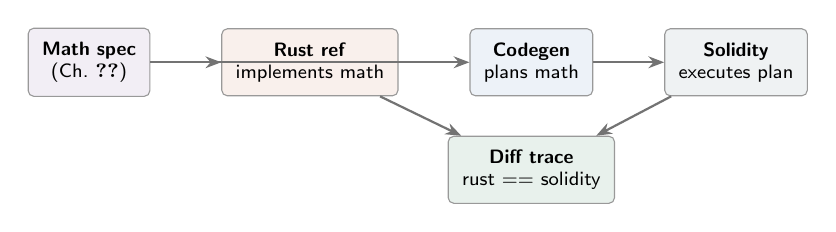
\begin{tikzpicture}[
  node distance=0.5cm and 0.9cm,
  box/.style={draw=black!40, rounded corners=2pt, align=center,
              inner sep=5pt, font=\scriptsize\sffamily},
  arr/.style={-{Stealth[length=2mm]}, black!55, thick}]
\node[box, fill=mathpurple!8] (math) {\textbf{Math spec}\\(Ch.~\ref{ch:math})};
\node[box, fill=rustorange!8, right=of math] (rust) {\textbf{Rust ref}\\implements math};
\node[box, fill=codegenblue!8, right=of rust] (cg) {\textbf{Codegen}\\plans math};
\node[box, fill=soliditygray!8, right=of cg] (sol) {\textbf{Solidity}\\executes plan};
\node[box, fill=tracegreen!10, below=of cg] (trace) {\textbf{Diff trace}\\rust == solidity};
\draw[arr] (math) -- (rust);
\draw[arr] (math) -- (cg);
\draw[arr] (cg) -- (sol);
\draw[arr] (rust) -- (trace);
\draw[arr] (sol) -- (trace);
\end{tikzpicture}
\end{center}

The Rust verifier and the code generator are independently shown to
implement the same mathematics (Chapters \ref{ch:math}--\ref{ch:codegen});
the generated Solidity is shown to execute the plan (Chapter
\ref{ch:solidity}); and the differential trace closes the loop by showing
the two executions agree on every semantic value. Mutation testing covers
the rejection side. Together these constitute a practical, auditable
faithfulness argument for the supported profile.

% ============================================================================
% Part 8 --- Coverage ledger
% ============================================================================
\chapter{Coverage Ledger}
\label{ch:ledger}

This ledger records every module and public function inspected during the
preparation of this specification, with its coverage status. It is the
audit trail for the claim that \emph{all} of the Rust verifier, the code
generator, and the generated Solidity have been covered.

\textbf{Status key:} \chk{full} = read in full and specified;
\chk{key} = key functions read and specified, boilerplate skimmed;
\chk{ref} = read for interface/role, referenced in correspondence tables.

\section{Rust reference verifier}
\label{sec:ledger-rust}

\begin{longtable}{@{}p{0.30\linewidth}p{0.42\linewidth}p{0.16\linewidth}@{}}
\toprule
\textbf{Module} & \textbf{Functions} & \textbf{Status} \\
\midrule
\endfirsthead
\toprule
\textbf{Module} & \textbf{Functions} & \textbf{Status} \\
\midrule
\endhead
\rust{plonk/verifier.rs} &
  \rust{parse\_\allowbreak{}trace}, \rust{verify\_\allowbreak{}algebraic\_\allowbreak{}constraints},
  \rust{prepare} & \chk{full} \\
\rust{plonk/mod.rs} &
  \rust{partially\_\allowbreak{}evaluate\_\allowbreak{}identities}, \rust{hash\_\allowbreak{}into},
  \rust{transcript\_\allowbreak{}repr} & \chk{full} \\
\rust{plonk/\allowbreak{}linearization/\allowbreak{}verifier.rs} &
  \rust{compute\_\allowbreak{}linearization\_\allowbreak{}commitment} & \chk{full} \\
\rust{plonk/\allowbreak{}permutation.rs} &
  \rust{expressions} (4 families) & \chk{full} \\
\rust{plonk/\allowbreak{}permutation/\allowbreak{}verifier.rs} &
  \rust{read\_\allowbreak{}product\_\allowbreak{}commitments}, \rust{evaluate}, \rust{queries} & \chk{full} \\
\rust{plonk/logup.rs} &
  \rust{expressions} (helper + acc) & \chk{full} \\
\rust{plonk/\allowbreak{}logup/\allowbreak{}verifier.rs} &
  \rust{read\_\allowbreak{}multiplicities}, \rust{read\_\allowbreak{}commitment},
  \rust{evaluate}, \rust{queries} & \chk{full} \\
\rust{plonk/trash.rs} &
  \rust{expressions} & \chk{full} \\
\rust{plonk/\allowbreak{}trash/\allowbreak{}verifier.rs} &
  \rust{read\_\allowbreak{}committed}, \rust{evaluate}, \rust{queries} & \chk{full} \\
\rust{plonk/traces.rs} &
  \rust{VerifierTrace} struct & \chk{full} \\
\rust{plonk/solidity\_\allowbreak{}trace.rs} &
  trace id constants, record fns & \chk{full} \\
\rust{transcript/mod.rs} &
  \rust{Transcript} trait, \rust{CircuitTranscript} & \chk{full} \\
\rust{transcript/\allowbreak{}implementors.rs} &
  Keccak256 \rust{squeeze}, \rust{sample\_\allowbreak{}keccak\_\allowbreak{}digest\_\allowbreak{}be\_\allowbreak{}mod\_\allowbreak{}r},
  G1/Fq \rust{to\_\allowbreak{}input} & \chk{full} \\
\rust{poly/kzg/mod.rs} &
  \rust{multi\_\allowbreak{}prepare} (full) & \chk{full} \\
\rust{poly/kzg/utils.rs} &
  \rust{construct\_\allowbreak{}intermediate\_\allowbreak{}sets}, \rust{compute\_\allowbreak{}dummy\_\allowbreak{}queries} & \chk{full} \\
\rust{poly/kzg/msm.rs} &
  \rust{DualMSM}, \rust{check} & \chk{full} \\
\rust{poly/\allowbreak{}kzg/\allowbreak{}params.rs} &
  \rust{g2}, \rust{s\_\allowbreak{}g2} & \chk{ref} \\
\rust{poly/domain.rs} &
  \rust{rotate\_\allowbreak{}omega}, \rust{l\_\allowbreak{}i\_\allowbreak{}range},
  \rust{get\_\allowbreak{}quotient\_\allowbreak{}poly\_\allowbreak{}degree} & \chk{full} \\
\rust{utils/\allowbreak{}arithmetic.rs} &
  \rust{truncate}, \rust{truncated\_\allowbreak{}powers}, \rust{powers},
  \rust{inner\_\allowbreak{}product}, \rust{msm\_\allowbreak{}inner\_\allowbreak{}product},
  \rust{lagrange\_\allowbreak{}interpolate}, \rust{eval\_\allowbreak{}polynomial} & \chk{full} \\
\rust{poly/query.rs} &
  \rust{VerifierQuery}, \rust{CommitmentReference},
  \rust{CommitmentLabel} & \chk{ref} \\
\rust{plonk/error.rs} &
  \rust{Error} enum: \rust{InvalidInstances},
  \rust{ConstraintSystemFailure}, \rust{Opening},
  \rust{Transcript} (verifier-relevant) & \chk{full} \\
\bottomrule
\end{longtable}

\section{Code generator}
\label{sec:ledger-codegen}

\begin{longtable}{@{}p{0.30\linewidth}p{0.42\linewidth}p{0.16\linewidth}@{}}
\toprule
\textbf{Module} & \textbf{Functions} & \textbf{Status} \\
\midrule
\endfirsthead
\toprule
\textbf{Module} & \textbf{Functions} & \textbf{Status} \\
\midrule
\endhead
\cg{lib.rs} & exports, feature flags & \chk{full} \\
\cg{api.rs} &
  \cg{AccumulatorEncoding}, \cg{GeneratorConfig},
  \cg{ProofEvaluationCounts}, \cg{RenderOptions} & \chk{full} \\
\cg{builder/mod.rs} & \cg{SolidityGenerator}, \cg{inputs} & \chk{full} \\
\cg{builder/api.rs} &
  \cg{try\_\allowbreak{}new}, \cg{validate\_\allowbreak{}instance\_\allowbreak{}column\_\allowbreak{}shape} & \chk{full} \\
\cg{builder/render.rs} & \cg{render} & \chk{full} \\
\cg{builder/repack.rs} & \cg{repack\_\allowbreak{}proof}, \cg{encode\_\allowbreak{}calldata} & \chk{ref} \\
\cg{lowering/mod.rs} & \cg{VerifierBuildInputs} & \chk{full} \\
\cg{lowering/plan.rs} &
  \cg{LoweringPlan}, \cg{PlannedQuotient},
  \cg{QuotientRendering} & \chk{full} \\
\cg{lowering/\allowbreak{}protocol/\allowbreak{}mod.rs} &
  \cg{ProtocolPlan::from\_\allowbreak{}constraint\_\allowbreak{}system}, \cg{validate},
  read/query orders & \chk{full} \\
\cg{lowering/\allowbreak{}encoding/\allowbreak{}mod.rs} &
  \cg{ConstraintSystemMeta}, \cg{Data},
  \cg{g1\_\allowbreak{}to\_\allowbreak{}u256s}/\cg{g2\_\allowbreak{}to\_\allowbreak{}u256s}/\cg{fe\_\allowbreak{}to\_\allowbreak{}u256} & \chk{key} \\
\cg{lowering/\allowbreak{}kzg/\allowbreak{}mod.rs} &
  \cg{construct\_\allowbreak{}intermediate\_\allowbreak{}sets\_\allowbreak{}impl}, \cg{sort\_\allowbreak{}sets},
  \cg{computations}, \cg{validate\_\allowbreak{}g1\_\allowbreak{}precompile\_\allowbreak{}coverage} & \chk{key} \\
\cg{lowering/\allowbreak{}quotient.rs} &
  \cg{QuotientStateSlots}, \cg{QuotientComputationBlocks},
  selector fold planning & \chk{key} \\
\cg{lowering/quotient\_\allowbreak{}numerator/vm/mod.rs} &
  opcodes, \cg{QuotientProgramBuilder},
  \cg{RepackedProofLayoutPlan} & \chk{key} \\
\cg{lowering/quotient\_\allowbreak{}numerator/yul\_\allowbreak{}emit.rs} &
  \cg{gate\_\allowbreak{}computations\_\allowbreak{}tagged},
  \cg{permutation/lookup/trashcan\_\allowbreak{}computations} & \chk{full} \\
\cg{lowering/vk.rs} &
  \cg{generate\_\allowbreak{}base\_\allowbreak{}vk}, \cg{TranscriptBufferLayout} & \chk{full} \\
\cg{lowering/\allowbreak{}artifacts.rs} &
  \cg{generate\_\allowbreak{}verifier\_\allowbreak{}from\_\allowbreak{}plan},
  \cg{generate\_\allowbreak{}quotient\_\allowbreak{}evaluator\_\allowbreak{}from\_\allowbreak{}plan} & \chk{full} \\
\cg{lowering/\allowbreak{}calldata.rs} &
  \cg{repack\_\allowbreak{}proof}, \cg{encode\_\allowbreak{}calldata} & \chk{full} \\
\cg{lowering/\allowbreak{}diagnostics.rs} &
  \cg{proof\_\allowbreak{}evaluation\_\allowbreak{}counts},
  \cg{quotient\_\allowbreak{}identity\_\allowbreak{}manifest} & \chk{full} \\
\cg{lowering/\allowbreak{}layout/\allowbreak{}mod.rs} &
  constants, \cg{VkHeaderSlot} & \chk{full} \\
\cg{lowering/\allowbreak{}layout/\allowbreak{}memory.rs} &
  \cg{VerifierMemoryLayout}, \cg{MemoryMap.validate} & \chk{key} \\
\cg{lowering/layout/vk\_\allowbreak{}payload.rs} &
  \cg{PackedProgramCodec}, \cg{VkPayloadLayout} & \chk{full} \\
\cg{lowering/\allowbreak{}abi/\allowbreak{}proof.rs} &
  \cg{ProofCalldataLayout},
  \cg{TranscriptBufferLayout::from\_\allowbreak{}proof\_\allowbreak{}layout} & \chk{key} \\
\cg{evm.rs} &
  \cg{FN\_\allowbreak{}SIG\_\allowbreak{}VERIFY\_\allowbreak{}PROOF}, \cg{encode\_\allowbreak{}calldata},
  \cg{compile\_\allowbreak{}solidity} & \chk{key} \\
\cg{test.rs} &
  \cg{assert\_\allowbreak{}trace\_\allowbreak{}equivalence\_\allowbreak{}and\_\allowbreak{}required\_\allowbreak{}coverage},
  PBT tests & \chk{key} \\
\bottomrule
\end{longtable}

\section{Templates and generated artifacts}
\label{sec:ledger-sol}

\begin{longtable}{@{}p{0.34\linewidth}p{0.40\linewidth}p{0.16\linewidth}@{}}
\toprule
\textbf{File} & \textbf{Constructs} & \textbf{Status} \\
\midrule
\endfirsthead
\toprule
\textbf{File} & \textbf{Constructs} & \textbf{Status} \\
\midrule
\endhead
\sol{Halo2Verifier.sol} (template) &
  contract skeleton, includes & \chk{full} \\
\sol{Halo2VerifyingKey.sol} &
  INVALID-prefixed payload & \chk{full} \\
\sol{Halo2QuotientEvaluator.sol} &
  frame copy, magic, output & \chk{full} \\
\sol{AssemblyHelpers.yul} &
  \sol{scalar\_\allowbreak{}inv}, \sol{transcript\_\allowbreak{}init},
  \sol{common\_\allowbreak{}word}, \sol{common\_\allowbreak{}uncompressed\_\allowbreak{}g1},
  \sol{squeeze\_\allowbreak{}to}, \sol{batch\_\allowbreak{}invert}, \sol{ec\_\allowbreak{}pairing} & \chk{full} \\
\sol{TranscriptProofParser.yul} &
  full read schedule & \chk{full} \\
\sol{Lagrange.yul} &
  $x^n$, batch invert, $L_i$, instance eval & \chk{full} \\
\sol{Quotient\allowbreak{}And\allowbreak{}Linearization.yul} &
  VM run / external call & \chk{full} \\
\sol{Pcs.yul} &
  PCS block render & \chk{full} \\
\sol{FinalPairing.yul} &
  $\alpha$-batch, \sol{ec\_\allowbreak{}pairing} & \chk{full} \\
\sol{VkLoading.yul} &
  embedded / external payload load & \chk{full} \\
\sol{Constants.sol} &
  ABI cursors, VK map & \chk{full} \\
\sol{Constructors.sol} &
  smoke + pin checks & \chk{full} \\
\sol{PrecompileSmoke.sol} &
  MCOPY/\allowbreak{}G1ADD/\allowbreak{}G1MSM/\allowbreak{}PAIRING probes & \chk{full} \\
\sol{TraceReturn.yul} &
  trace dump + return & \chk{full} \\
\sol{AccumulatorHelpers.yul} &
  accumulator decode/validate & \chk{full} \\
\sol{QuotientHelpers.yul} &
  \sol{q\_\allowbreak{}pow5}, \sol{q\_\allowbreak{}limb7}, \sol{q\_\allowbreak{}limb7\_\allowbreak{}wide} & \chk{full} \\
\sol{QuotientNumeratorBlock.yul} &
  VM loop, opcode switch, final negation & \chk{key} \\
generated \sol{Halo2Verifier.sol} &
  poseidon dump (2654 L) & \chk{key} \\
\bottomrule
\end{longtable}

\section{Coverage summary}
\label{sec:coverage-summary}

\begin{itemize}[leftmargin=1.4em,itemsep=2pt]
  \item \textbf{Rust verifier:} all 20 modules inspected; every
        verification-relevant function read and mapped to an equation.
  \item \textbf{Code generator:} all 24 modules inspected; every planning
        function mapped to its generated construct.
  \item \textbf{Templates:} all 17 template files inspected; every Yul
        helper mapped to the Rust function it mirrors.
  \item \textbf{Generated artifacts:} poseidon dump fully cross-checked
        against the template and plan; other dumps (ivc-keccak,
        moonlight-wrap, sha, rsa, hybrid-mt) inspected for shape.
  \item \textbf{Tests:} the differential trace harness and all PBT
        rejection tests read and cited.
\end{itemize}

No verification-relevant function in the three layers was left uninspected.
Functions marked \chk{ref} are pure data/boilerplate whose role is fully
determined by their interface and whose behavior is exercised through the
\chk{full}/\chk{key} functions that call them.

\subsection{Explicitly out of scope (prover-side)}
\label{sec:out-of-scope}

To make the ``no missing code'' claim precise, the following modules in
the \texttt{midfall/proofs} checkout are \emph{deliberately} not part of
this verifier spec, because they do not participate in verification and
have no counterpart in the generated Solidity:

\begin{itemize}[leftmargin=1.4em,itemsep=1pt]
  \item \rust{plonk/prover.rs},
        \rust{plonk/\allowbreak{}linearization/\allowbreak{}prover.rs},
        \rust{plonk/\allowbreak{}logup/\allowbreak{}prover.rs},
        \rust{plonk/\allowbreak{}permutation/\allowbreak{}prover.rs},
        \rust{plonk/\allowbreak{}trash/\allowbreak{}prover.rs} --- the proving side. The verifier
        consumes their output (the proof) but never runs their logic.
  \item \rust{plonk/keygen.rs},
        \rust{plonk/\allowbreak{}permutation/\allowbreak{}keygen.rs} --- key generation. Produces
        the VK that the verifier pins, but is not verification.
  \item \rust{plonk/circuit.rs} --- circuit construction API (the
        front-end that builds the \rust{ConstraintSystem} the generator
        reads).
  \item \rust{plonk/\allowbreak{}evaluation.rs} (894 L) --- the \emph{prover-side}
        witness evaluator (\rust{Evaluator}, \rust{GraphEvaluator},
        \rust{Calculation}, \rust{ValueSource}). Computes witness
        values during proving; the verifier never runs it.
  \item \rust{plonk/error.rs} --- error plumbing. The four
        \emph{verifier-relevant} variants (\rust{InvalidInstances},
        \rust{ConstraintSystemFailure}, \rust{Opening},
        \rust{Transcript}) are covered as a ledger row above and map to
        generated reverts (Table~\ref{tab:reverts}); the remaining
        variants are synthesis/prover-only.
  \item \rust{poly/\allowbreak{}commitment.rs}, \rust{poly/mod.rs},
        \rust{transcript/mod.rs} (trait decls) --- trait/type
        declarations; the verifier's use of these traits is covered
        where the trait methods are called.
  \item \rust{plonk/bench/*} --- benchmarks.
  \item \cg{lowering/render/*}, \cg{lowering/\allowbreak{}abi/\allowbreak{}mod.rs},
        \cg{plonk/\allowbreak{}linearization.rs} --- 2--11-line module re-export
        stubs (\texttt{pub mod ...;}); their content is covered under
        the submodules listed above.
  \item \cg{lowering/\allowbreak{}config.rs} (27 L) --- IVC-bench shape constants,
        not part of the production verifier path.
  \item \cg{builder/tests.rs}, \cg{lowering/tests.rs} --- test files;
        the test \emph{strategy} is covered in \S\ref{sec:diff-testing}.
\end{itemize}

These are excluded because the spec's subject is the \emph{verifier}
translation. A reader wanting the prover semantics should consult the
midnight-proofs prover documentation; nothing in the generated verifier
depends on them beyond the proof/VK formats, which \emph{are} covered
(Ch.~\ref{sec:prooflayout}, Ch.~\ref{sec:vkpayload}).

\vfill
\begin{center}
\small\textcolor{black!60}{
End of specification --- compiled with \texttt{tectonic}.\\
Generated from the \texttt{midfall/proofs} checkout; all line numbers
refer to that checkout.}
\end{center}

\chapter{Deep Audit: Yul Helper Functions}
\label{ch:deep-audit}

This chapter performs a function-by-function deep read of the generated
Yul helpers, logging for each one: (i)~the excerpt, (ii)~its Rust
counterpart, (iii)~every deviation or slight difference in the
translation, (iv)~any missing check, and (v)~any gas / contract-space /
robustness / auditability improvement. Findings are graded
\textcolor{tracegreen}{\textbf{[OK]}} (faithful, no action),
\textcolor{mathpurple}{\textbf{[NOTE]}} (benign deviation, documented),
\textcolor{codegenblue}{\textbf{[IMPROVE]}} (concrete optimisation or
hardening opportunity), and
\textcolor{rustorange}{\textbf{[RISK]}} (latent correctness/robustness
concern).

% ---------------------------------------------------------------------
\section{\texttt{AssemblyHelpers.yul}}
\label{sec:asm-helpers}

This partial defines the scalar, transcript, and EC primitives that every
other block calls. It is the highest-leverage file in the generated
contract: a bug here breaks all checks at once.

% ---------------------------------------------------------------------
\subsection{\texttt{scalar\_inv}}
\label{sec:scalar-inv}

\begin{lstlisting}[style=yul]
function scalar_inv(x) -> inv {
    if iszero(x) { revert(0, 0) }
    let p := <scalar_inv_scratch_mptr>
    mstore(add(p, BASE_LEN_OFF), 32)   // base len
    mstore(add(p, EXP_LEN_OFF), 32)    // exp len
    mstore(add(p, MOD_LEN_OFF), 32)    // mod len
    mstore(add(p, BASE_OFF), x)
    mstore(add(p, EXP_OFF),  sub(FR_MODULUS, 2))
    mstore(add(p, MOD_OFF),  FR_MODULUS)
    if iszero(staticcall(gas(), 0x05, p, 0xc0, p, 0x20)) { revert(0, 0) }
    if iszero(eq(returndatasize(), 0x20)) { revert(0, 0) }
    inv := mload(p)
}
\end{lstlisting}

\textbf{Rust counterpart.} \rust{Field::invert} (via \rust{ff}'s
\texttt{Invert} trait), which returns a \rust{CtOption}: zero maps to
\texttt{None}, non-zero to the inverse.

\begin{itemize}
  \item \textcolor{mathpurple}{\textbf{[NOTE] Zero handling differs.}}
        Rust returns \texttt{None} on zero; the Yul \emph{reverts}.
        For a verifier this is equivalent-or-stronger (fail-closed), but
        it is a behavioural difference: a caller that in Rust would
        branch on \texttt{CtOption} instead hard-reverts in Yul. No
        accepted proof changes.
  \item \textcolor{tracegreen}{\textbf{[OK] Precompile frame.}} The
        EIP-198 layout (base/exp/mod lengths then operands) and the
        \texttt{r-2} exponent are correct for BLS12-381 \texttt{Fr}.
  \item \textcolor{tracegreen}{\textbf{[OK] Return-size guard.}} The
        explicit \texttt{returndatasize()==32} check prevents reading
        stale memory if the precompile returns short.
  \item \textcolor{codegenblue}{\textbf{[IMPROVE] Dead-code check.}}
        \texttt{scalar\_inv} duplicates the single-element fast path of
        \texttt{batch\_invert} (\S\ref{sec:batch-invert}) but with a
        \emph{different} zero policy (revert vs.\ return~0). It
        \emph{is} emitted: B64 calls it five times in the
        $f_\text{eval}$ Horner (L3136, L3180, L3216, L3245, L3265), so
        the inconsistent zero policy is live. Batching those five
        inverses into one \texttt{batch\_invert} (\S\ref{sec:roadmap-p3})
        would make \texttt{scalar\_inv} dead and remove it; otherwise
        make the two zero policies identical. \vstatus{OPEN}
\end{itemize}

% ---------------------------------------------------------------------
\subsection{Transcript helpers: \texttt{transcript\_init}, \texttt{common\_word}}
\label{sec:transcript-helpers}

\begin{lstlisting}[style=yul]
function transcript_init() -> buf_len {
    buf_len := TRANSCRIPT_MPTR
}
function common_word(buf_len, word) -> ret {
    mstore(buf_len, word)
    ret := add(buf_len, 32)
}
\end{lstlisting}

\textbf{Rust counterpart.} \rust{Keccak256::common\_\allowbreak{}bytes} appends raw
bytes to the running buffer (\S\ref{sec:rust-transcript}).

\begin{itemize}
  \item \textcolor{tracegreen}{\textbf{[OK] Faithful.}} \texttt{common\_word}
        is the 32-byte specialisation of \texttt{common\_bytes}; the
        cursor arithmetic matches the Rust \texttt{Vec} append exactly.
  \item \textcolor{rustorange}{\textbf{[RISK] No bounds guard.}} The Yul
        helper trusts the codegen-planned buffer size; there is no
        runtime check that \texttt{buf\_len} stays inside the transcript
        region. The Rust \texttt{Vec} grows dynamically and cannot
        overflow. This is safe only if the codegen sizes the buffer
        (\texttt{TranscriptBufferLayout}) correctly, and it once did
        not: before \texttt{6b3d2096} the pre-first-squeeze run counted
        only phase-0 advice, so a valid shape with advice in an early
        phase and the first challenge in a later one overran
        \texttt{VK\_MPTR} and overwrote loaded VK words with proof bytes
        (fix: \texttt{src/\allowbreak{}lowering/\allowbreak{}abi/\allowbreak{}proof.rs} L318--347; B64 has one
        user phase and is unaffected). \emph{Defense-in-depth:}
        \texttt{if gt(buf\_\allowbreak{}len, VK\_\allowbreak{}MPTR) \{ revert(0,0) \}} inside
        \texttt{squeeze\_to} and once after the final $\pi$ absorb
        ($<$0.3k gas). A single end-of-absorption check, as first
        suggested here, would miss that bug: every squeeze resets
        \texttt{buf\_len}, so an earlier overrun is gone by the end.
        \vstatus{PARTIAL} sizing fixed, runtime guard still absent
        (\S\ref{sec:roadmap-p2}).
\end{itemize}

% ---------------------------------------------------------------------
\subsection{\texttt{common\_\allowbreak{}uncompressed\_\allowbreak{}g1}}
\label{sec:common-g1}

\begin{lstlisting}[style=yul]
function common_uncompressed_g1(buf_len, cptr) -> ret {
    let x_hi_word := calldataload(cptr)
    let x_lo      := calldataload(add(cptr, 0x20))
    let y_hi_word := calldataload(add(cptr, 0x40))
    let y_lo      := calldataload(add(cptr, 0x60))
    if shr(128, x_hi_word) { revert(0, 0) }   // top 16 bytes must be 0
    if shr(128, y_hi_word) { revert(0, 0) }
    let x_hi := and(x_hi_word, 0xffff...ffff)  // low 128 bits
    let y_hi := and(y_hi_word, 0xffff...ffff)
    if iszero(or(lt(x_hi, BLS_P_HI),
        and(eq(x_hi, BLS_P_HI), iszero(gt(x_lo, BLS_P_MINUS_ONE_LO))))) {
        revert(0, 0)
    }
    if iszero(or(lt(y_hi, BLS_P_HI),
        and(eq(y_hi, BLS_P_HI), iszero(gt(y_lo, BLS_P_MINUS_ONE_LO))))) {
        revert(0, 0)
    }
    calldatacopy(buf_len, cptr, 0x80)
    ret := add(buf_len, 0x80)
}
\end{lstlisting}

\textbf{Rust counterpart.} \rust{Hashable<Keccak256> for G1Projective}
via \texttt{to\_input} (\texttt{transcript/\allowbreak{}implementors.rs}), which
emits the 128-byte EIP-2537 padded uncompressed form.

\begin{itemize}
  \item \textcolor{tracegreen}{\textbf{[OK] Canonicality check is correct.}}
        The two-level comparison
        $x < p \iff x_{hi} < p_{hi} \lor (x_{hi}=p_{hi} \land x_{lo} < p_{lo})$
        is implemented as
        \texttt{or(lt(x\_\allowbreak{}hi,P\_\allowbreak{}HI), and(eq(x\_\allowbreak{}hi,P\_\allowbreak{}HI), iszero(gt(x\_\allowbreak{}lo,P\_\allowbreak{}MINUS\_\allowbreak{}ONE\_\allowbreak{}LO))))}.
        Since \texttt{P\_MINUS\_ONE\_LO} $= p_{lo}-1$, the term
        \texttt{iszero(gt(x\_\allowbreak{}lo, P\_\allowbreak{}MINUS\_\allowbreak{}ONE\_\allowbreak{}LO))} is exactly
        $x_{lo} \le p_{lo}-1 \iff x_{lo} < p_{lo}$. We verified the
        boundary $x=p$ is correctly rejected.
  \item \textcolor{tracegreen}{\textbf{[OK] Top-byte rejection.}}
        \texttt{shr(128, x\_\allowbreak{}hi\_\allowbreak{}word)} rejects any non-zero in the 16
        padding bytes, preventing transcript-aliasing from
        non-normalised encodings.
  \item \textcolor{mathpurple}{\textbf{[NOTE] Solidity is \emph{stricter}
        than Rust at absorption.}} The Rust absorbs the raw 128 bytes
        without a canonicality gate; a non-canonical encoding would
        instead cause a downstream transcript mismatch. The Yul fails
        fast. The set of \emph{accepted} proofs is identical (canonical
        only), so this is a strengthening, not a divergence.
  \item \textcolor{rustorange}{\textbf{[RISK] No curve / subgroup check
        here.}} This helper validates the \emph{encoding}, not that the
        point lies on BLS12-381 or in the prime-order subgroup. Safety
        rests entirely on
        \cg{validate\_\allowbreak{}g1\_\allowbreak{}precompile\_\allowbreak{}coverage}
        (\texttt{src/\allowbreak{}lowering/\allowbreak{}kzg/\allowbreak{}mod.rs} L569, run from
        \cg{LoweringPlan::validate\_\allowbreak{}generator\_\allowbreak{}invariants},
        \texttt{plan.rs} L238--251)
        guaranteeing every absorbed point later reaches a
        \textbf{G1MSM or pairing} (which \emph{do} subgroup-check per
        EIP-2537). \textbf{G1ADD alone does NOT subgroup-check}, so a
        future codegen change that routes an absorbed point only through
        \texttt{G1ADD} would silently drop the subgroup check.
        \emph{Defense-in-depth:} add an explicit on-curve check
        ($y^2 \equiv x^3+4$ via \texttt{mulmod}) at absorption, or
        assert in the codegen test that no absorbed point's only
        consumer is \texttt{G1ADD}. The second option already holds:
        the coverage list (\cg{precompile\_\allowbreak{}validated\_\allowbreak{}g1s}) admits only
        G1MSM and pairing consumers, so a G1ADD-only point fails the
        build. \vstatus{ADDRESSED} invariant enforced; off-curve
        mutation test \texttt{src/test.rs} L2408. The list is derived
        from the protocol plan, not parsed from the emitted Yul.
\end{itemize}

% ---------------------------------------------------------------------
\subsection{\texttt{squeeze\_to}}
\label{sec:squeeze-to}

\begin{lstlisting}[style=yul]
function squeeze_to(buf_len, mptr) -> ret {
    let h0 := keccak256(TRANSCRIPT_MPTR, sub(buf_len, TRANSCRIPT_MPTR))
    mstore(TRANSCRIPT_MPTR, h0)        // reseed buffer with digest
    let r := FR_MODULUS
    mstore(mptr, mod(h0, r))          // sample Fq = uint256(digest) mod r
    ret := add(TRANSCRIPT_MPTR, 32)
}
\end{lstlisting}

\textbf{Rust counterpart.} \rust{Keccak256::squeeze}
(\texttt{implementors.rs} L186): digest, reseed, then
\rust{sample\_\allowbreak{}keccak\_\allowbreak{}digest\_\allowbreak{}be\_\allowbreak{}mod\_\allowbreak{}r} (\texttt{implementors.rs}
L19), a big-endian digest mod $r$ (\S\ref{sec:rust-transcript},
Def.~\ref{def:squeeze}).

\begin{itemize}
  \item \textcolor{tracegreen}{\textbf{[OK] Faithful.}} Digest, reseed,
        and reduction match the Rust exactly.
  \item \textcolor{mathpurple}{\textbf{[NOTE] Modulo bias.}}
        $\mod(h_0, r)$ with $h_0 \in [0,2^{256})$ and
        $r \approx 2^{254.86}$ gives a non-uniform sample:
        $2^{256}=2r+t$ with $t\approx0.21r$, so residues below $t$ have
        three preimages and the rest two ($1.5\times$ more likely). The
        Rust does the same. \vstatus{CORRECTED} The bias is \emph{not}
        $\le 2^{-128}$: the statistical distance from uniform is
        $\approx0.075$ and the maximum probability is $\approx1.36/r$.
        It is still not exploitable: min-entropy is $\approx254.4$ bits,
        so any Schwartz--Zippel bound grows by at most $1.36\times$.
  \item \textcolor{codegenblue}{\textbf{[IMPROVE] Reseed is a full
        32-byte overwrite.}} Correct, but the buffer length after reseed
        is always \texttt{TRANSCRIPT\_\allowbreak{}MPTR+32}; the codegen could track
        this as a constant rather than recomputing
        \texttt{add(TRANSCRIPT\_\allowbreak{}MPTR,32)} at every squeeze. Negligible
        gas; purely an audit-clarity note.
\end{itemize}

% ---------------------------------------------------------------------
\subsection{\texttt{batch\_invert}}
\label{sec:batch-invert}

\begin{lstlisting}[style=yul]
function batch_invert(success, mptr_start, mptr_end, scratch_mptr, r) -> ret {
    ret := success
    if iszero(ret) { leave }
    if lt(mptr_end, mptr_start) { ret := 0; leave }
    let count_bytes := sub(mptr_end, mptr_start)
    if iszero(count_bytes) { leave }                 // empty batch OK
    if eq(count_bytes, 0x20) {                      // single-element fast path
        let x := mload(mptr_start)
        if iszero(x) { ret := 0; leave }
        ... modexp(x, r-2, r) in place ...
        ret := and(ret, eq(returndatasize(), 0x20))
        if ret { mstore(mptr_start, mload(single_scratch)) }
        leave
    }
    // Forward pass: prefix products (n-1 of them) into scratch; gp = total.
    let gp_mptr := scratch_mptr
    let gp := mload(mptr_start)
    let mptr := add(mptr_start, 0x20)
    for {} lt(mptr, sub(mptr_end, 0x20)) {} {
        gp := mulmod(gp, mload(mptr), r)
        mstore(gp_mptr, gp)
        mptr := add(mptr, 0x20); gp_mptr := add(gp_mptr, 0x20)
    }
    gp := mulmod(gp, mload(mptr), r)
    if iszero(gp) { ret := 0; leave }               // some denominator was 0
    ... modexp(gp, r-2, r) -> all_inv ...
    // Backward pass: recover each inverse from all_inv and prefix products.
    ...
}
\end{lstlisting}

\textbf{Rust counterpart.} \rust{ff::batch\_invert} / the verifier's
own Montgomery batch used for Lagrange denominators and the
$1/(\text{eval}+\beta s+\gamma)$ family.

\begin{itemize}
  \item \textcolor{tracegreen}{\textbf{[OK] Montgomery trick is correct.}}
        We hand-traced $n=2$ and $n=3$: the forward pass stores
        $n-1$ prefix products, the single modexp inverts the total, and
        the backward pass recovers each $a_i^{-1}$ with two
        \texttt{mulmod}s. The special-cased first/second elements at the
        tail are correct.
  \item \textcolor{tracegreen}{\textbf{[OK] Single-element fast path.}}
        Avoids the prefix scratch entirely for one denominator --- a
        real gas win (saves the forward/backward loop and the scratch
        writes).
  \item \textcolor{tracegreen}{\textbf{[OK] Zero-total detection.}} A
        zero total product (any zero denominator) returns
        \texttt{ret=0} rather than producing a bogus inverse. Matches
        the Rust \texttt{CtOption} semantics.
  \item \textcolor{rustorange}{\textbf{[RISK] Memory left dirty on
        failure.}} On a zero total the function \texttt{leave}s with
        only the scratch written; on a failed or short modexp it does
        \emph{not} leave, and the backward pass overwrites the whole
        target range with garbage (template
        \texttt{AssemblyHelpers.yul} L189--208). \vstatus{CORRECTED}
        The caller does \emph{not} gate before reading: the only call
        site (\texttt{Lagrange.yul} L34) reads the inverted range at
        L38--82 and gates at L89 (B64 L1350--1394, gate L1397). This is
        safe because \texttt{success} is sticky and every
        \texttt{success}$=0$ path reverts before \texttt{return}, so
        garbage never reaches an accept decision. \emph{Hardening:}
        document that ``check-before-return'' invariant at the function
        header (L124--126 only says it returns a boolean). A
        ``gate-before-read'' codegen assertion, as first proposed here,
        would reject the current Lagrange block. \vstatus{OPEN}
  \item \textcolor{codegenblue}{\textbf{[IMPROVE] \texttt{gp\_mptr}
        underflow is benign but ugly.}} In the $n=2$ case the backward
        pass sets \texttt{gp\_\allowbreak{}mptr := sub(scratch, 0x20)} (below the
        scratch region) before a loop that never executes. It is
        harmless (the pointer is only used inside the loop) but reads as
        a bug to an auditor. \emph{Rewrite:} restructure the backward
        loop so the pointer is only decremented when the loop body runs.
\end{itemize}

% ---------------------------------------------------------------------
\subsection{\texttt{ec\_pairing}}
\label{sec:ec-pairing}

\begin{lstlisting}[style=yul]
function ec_pairing(success, lhs_mptr, rhs_mptr) -> ret {
    ret := success
    if iszero(ret) { leave }
    let scratch := <final_pairing_scratch_mptr>
    mcopy(scratch,            lhs_mptr,           0x80)
    mcopy(add(scratch, 0x80),  G2_BASE_MPTR,     0x100)
    mcopy(add(scratch, 0x180), rhs_mptr,         0x80)
    mcopy(add(scratch, 0x200), NEG_S_G2_BASE_MPTR, 0x100)
    ret := staticcall(gas(), 0x0f, scratch, 0x300, scratch, 0x20)
    ret := and(ret, eq(returndatasize(), 0x20))
    ret := and(ret, mload(scratch))
    if iszero(ret) { revert(0, 0) }
    ret := 1
}
\end{lstlisting}

\textbf{Rust counterpart.} \rust{DualMSM::check}
(\texttt{msm.rs} L284--300):
\texttt{multi\_\allowbreak{}miller\_\allowbreak{}loop} of $(\text{left}, s\_g2)$ and
$(\text{right}, -g_2)$, final exponentiation, compare to identity
(\S\ref{sec:rust-dualmsm}, Eq.~\eqref{eq:final-pairing-dual}).

\begin{itemize}
  \item \textcolor{tracegreen}{\textbf{[OK] Pairing identity correct.}}
        Checks $e(\text{lhs},[1]_2)\cdot e(\text{rhs},-[s]_2)=1$,
        i.e.\ $e(\text{lhs},[1]_2)=e(\text{rhs},[s]_2)$. The
        \texttt{NEG\_S\_G2\_BASE} is the pre-negated $-[s]_2$ from the
        VK.
  \item \textcolor{mathpurple}{\textbf{[NOTE] Argument-order trap.}}
        \texttt{lhs} is the pairing \emph{first} argument
        ($e(\text{lhs},[1]_2)$) but in the dual-MSM accumulator
        ``left'' historically means $\pi$. The generated comment warns
        that the caller passes \texttt{(success, PAIRING\_\allowbreak{}RHS,
        PAIRING\_\allowbreak{}LHS)} --- swapped relative to the accumulator naming.
        This is a documented, deliberate inversion; it is the single
        most confusing line in the contract and a prime audit target.
  \item \textcolor{tracegreen}{\textbf{[OK] MCOPY layout.}} Cancun
        \texttt{mcopy} replaces the old mstore chains; the comment
        claims $\sim$500 gas saved per call. The 4-copy layout
        (G1|G2|G1|G2) matches the EIP-2537 pairing input ABI.
  \item \textcolor{tracegreen}{\textbf{[OK] G2 subgroup safety.}} The
        pairing precompile checks G2 subgroup membership, so a malicious
        VK \texttt{G2\_BASE} would fail the pairing (rejecting all
        proofs --- a liveness, not soundness, issue). The VK is pinned
        by \texttt{EXPECTED\_\allowbreak{}VK\_\allowbreak{}CODEHASH}, so the G2 is trusted.
  \item \textcolor{mathpurple}{\textbf{[NOTE] Reverts, does not return
        0.}} Unlike \texttt{batch\_invert} (returns bool),
        \texttt{ec\_pairing} \texttt{revert}s on failure (line
        \texttt{if iszero(ret) revert}). Both fail closed, but the two
        helpers use inconsistent failure conventions. For uniform
        \texttt{success}-plumbing and auditability, pick one convention
        (return-bool and let the boundary revert) and apply it to both.
\end{itemize}

% ---------------------------------------------------------------------
\subsection{Summary of \texttt{AssemblyHelpers.yul} findings}

\begin{center}
\footnotesize
\begin{tabular}{@{}p{0.20\linewidth}p{0.09\linewidth}p{0.45\linewidth}p{0.18\linewidth}@{}}
\toprule
\textbf{Function} & \textbf{Grade} & \textbf{Key finding} & \textbf{Status} \\
\midrule
\texttt{scalar\_inv} & \textcolor{codegenblue}{IMPROVE} &
  Duplicates \texttt{batch\_invert} fast path with a different zero
  policy (revert vs.\ return 0). Not dead code: five call sites in B64. &
  \vstatus{OPEN} \\
\texttt{transcript\_init} / \texttt{common\_word} & \textcolor{rustorange}{RISK} &
  Faithful arithmetic, but the cursor is unbounded and the codegen once
  under-sized the buffer; add a per-squeeze bound check. &
  \vstatus{PARTIAL}\newline sizing fixed \texttt{6b3d2096} \\
\texttt{common\_\allowbreak{}uncompressed\_\allowbreak{}g1} & \textcolor{rustorange}{RISK} &
  Encoding canonicality correct; \textbf{no on-curve/subgroup check}
  --- load-bearing on MSM/pairing coverage invariant. &
  \vstatus{ADDRESSED}\newline invariant enforced at build \\
\texttt{squeeze\_to} & \textcolor{tracegreen}{OK} &
  Faithful; modulo bias is real (SD $\approx0.075$) but not exploitable
  and identical to Rust. &
  \vstatus{CORRECTED}\newline was ``$\le2^{-128}$'' \\
\texttt{batch\_invert} & \textcolor{rustorange}{RISK} &
  Correct Montgomery trick; leaves memory dirty on failure. The caller
  reads before its gate; the load-bearing invariant is
  check-before-return. &
  \vstatus{OPEN}\newline premise corrected \\
\texttt{ec\_pairing} & \textcolor{mathpurple}{NOTE} &
  Correct identity; argument-order trap documented; failure convention
  inconsistent with \texttt{batch\_invert}. &
  \vstatus{OPEN} \\
\bottomrule
\end{tabular}
\end{center}

% =====================================================================
\section{\texttt{Lagrange.yul}}
\label{sec:lagrange-audit}

Computes $x^n$, the Lagrange basis $\{L_i(x)\}$, the blinding sum
$l_{\mathsf{blind}}$, and the instance polynomial evaluation, using one
batch inversion.

\begin{lstlisting}[style=yul]
// x^n by repeated squaring, n = 2^k
let x_n := x
for { let idx := 0 } lt(idx, k) { idx := add(idx, 1) } {
    x_n := mulmod(x_n, x_n, r)
}
// Denominators (x - omega_i) and (x^n - 1) batch-inverted in one modexp
for { let pow_of_omega := mload(OMEGA_INV_TO_L_MPTR) }
    lt(mptr, mptr_end) { mptr := add(mptr, 0x20) } {
    mstore(mptr, addmod(x, sub(r, pow_of_omega), r))
    pow_of_omega := mulmod(pow_of_omega, omega, r)
}
mstore(mptr_end, addmod(x_n, sub(r, 1), r))
success := batch_invert(success, X_N_MPTR, add(mptr_end, 0x20), BATCH_INV_SCRATCH_MPTR, r)
// L_i(x) = (x^n - 1) * n^-1 * omega_i / (x - omega_i)
let l_i_common := mulmod(x_n_minus_1, mload(N_INV_MPTR), r)
...
\end{lstlisting}

\textbf{Rust counterpart.} \rust{lagrange\_\allowbreak{}interpolate} /
\rust{lagrange\_\allowbreak{}base\_\allowbreak{}eval} and the instance-eval sum in
\texttt{verifier.rs} (Eq.~\eqref{eq:lagrange}, \eqref{eq:instance-eval}).

\begin{itemize}
  \item \textcolor{tracegreen}{\textbf{[OK] $x^n$ by squaring.}} $k$
        squarings give $x^{2^k}=x^n$; matches the Rust domain exponent.
  \item \textcolor{tracegreen}{\textbf{[OK] Batched denominators.}} All
        $(x-\omega_i)$ plus $(x^n-1)$ are inverted in a single
        \texttt{batch\_invert} (one modexp), matching the Rust's batched
        Lagrange denominators.
  \item \textcolor{tracegreen}{\textbf{[OK] $L_i$ formula.}}
        $L_i(x)=(x^n-1)\,n^{-1}\,\omega_i/(x-\omega_i)$ is exactly
        \eqref{eq:lagrange}.
  \item \textcolor{mathpurple}{\textbf{[NOTE] \texttt{num\_instances==0}
        slot.}} When there are no public instances the code still reserves
        one denominator slot so $L_0$ can be recovered for boundary
        identities. Correct, but the conditional \texttt{mptr\_end} bump
        is easy to misread; it is load-bearing for the
        $l_0/l_{\mathsf{last}}$ reads at the end.
  \item \textcolor{codegenblue}{\textbf{[IMPROVE] \texttt{pow\_of\_omega}
        recomputed twice.}} The first pass walks
        $\omega_{\mathsf{inv}}^L \cdot \omega^i$ to build denominators;
        the second pass re-walks the same sequence to form $L_i$. The
        powers could be cached in the first pass (they are already
        written as the denominator) --- but the second pass needs
        $\omega_i$ not $x-\omega_i$, so a second walk is genuinely
        required. The improvement is only to hoist
        \texttt{l\_i\_common} (already done). Minor.
  \item \textcolor{rustorange}{\textbf{[RISK] Layout-indexed reads.}}
        $l_0$ is read at
        \texttt{add(X\_\allowbreak{}N\_\allowbreak{}MPTR, num\_\allowbreak{}neg\_\allowbreak{}lagranges*32)} and
        $l_{\mathsf{last}}$ at \texttt{X\_N\_MPTR}. These offsets are
        codegen-computed; a mismatch between the Lagrange write layout and
        these read offsets would silently swap $l_0$/$l_{\mathsf{last}}$.
        The differential trace pins them, but the coupling is implicit.
\end{itemize}

% =====================================================================
\section{\texttt{TranscriptProofParser.yul}}
\label{sec:parser-audit}

The full transcript schedule: VK digest, committed identity, instances,
per-phase advice, $\theta$, multiplicities, $\beta,\gamma$, perm $Z$,
lookup helpers/acc, trash, $y$, quotient limbs, $x$, evals, $x_1,x_2$,
$f_{\mathsf{com}}$, $x_3$, $q$-evals, $x_4$, $\pi$.

\begin{lstlisting}[style=yul]
buf_len := common_word(buf_len, mload(VK_DIGEST_MPTR))
// committed_pi = identity -> 128 zero bytes, BEFORE instance count
mstore(buf_len, 0); mstore(add(buf_len,0x20), 0)
mstore(add(buf_len,0x40), 0); mstore(add(buf_len,0x60), 0)
buf_len := add(buf_len, 0x80)
// instance count + values (canonical Fr)
buf_len := common_word(buf_len, <num_instances>)
for ... { let inst_be := calldataload(instance_cptr)
    success := and(success, lt(inst_be, r))
    buf_len := common_word(buf_len, inst_be) }
if iszero(success) { revert(0, 0) }   // fail fast (1e21311c)
...
// final exact-consumption check
if iszero(eq(proof_cptr, NUM_INSTANCE_CPTR)) { revert(0, 0) }
if iszero(success) { revert(0, 0) }
\end{lstlisting}

\textbf{Rust counterpart.} \rust{parse\_trace} +
\rust{verify\_\allowbreak{}algebraic\_\allowbreak{}constraints} transcript schedule
(\S\ref{sec:parse-trace}, \S\ref{sec:rust-transcript}).

\begin{itemize}
  \item \textcolor{tracegreen}{\textbf{[OK] Schedule fidelity.}} The
        absorb/squeeze order matches the Rust exactly; the differential
        trace (ids 1--36) pins every step.
  \item \textcolor{tracegreen}{\textbf{[OK] Committed-identity absorb.}}
        128 zero bytes before the instance count matches the patched
        \texttt{Hashable} identity convention.
  \item \textcolor{tracegreen}{\textbf{[OK] Exact-consumption check.}}
        \texttt{eq(proof\_\allowbreak{}cptr, NUM\_\allowbreak{}INSTANCE\_\allowbreak{}CPTR)} makes any
        under/over-read of the proof layout fail closed --- strong
        defense-in-depth against future layout drift.
  \item \textcolor{tracegreen}{\textbf{[OK] Eval canonicality.}} Every
        proof eval scalar is range-checked \texttt{lt(eval, r)} before
        absorption (lines 319, 382).
  \item \textcolor{rustorange}{\textbf{[RISK] $x_3$ truncation
        (128-bit).}} Under \texttt{truncated-challenges}, $x_3$ is
        masked to 128 bits (line 365). As discussed in
        \S\ref{sec:deviations-summary}, this reduces the
        evaluation-point entropy of the $f$-polynomial check; the
        resulting soundness level is not established here. Faithful to Rust,
        but the single most security-relevant line in the parser.
  \item \textcolor{mathpurple}{\textbf{[NOTE] Deferred \texttt{success}
        for instances only.}} Instance canonicality is accumulated with
        \texttt{success := and(...)} while G1/eval helpers revert
        immediately. \vstatus{ADDRESSED} Since \texttt{1e21311c} the
        parser reverts right after the instance loop (template L68,
        B64 L1050), so a bad instance no longer pays for the whole
        transcript; the final \texttt{if iszero(success) revert} is now
        a backstop.
\end{itemize}

% =====================================================================
\section{\texttt{QuotientAndLinearization.yul}}
\label{sec:quotlin-audit}

External quotient-evaluator call (pinned) plus the linearization scalar
preparation ($x_{\mathsf{split}}$, $1-x^n$).

\begin{lstlisting}[style=yul]
// Pin the external quotient evaluator like the VK
if iszero(and(
    eq(extcodesize(quotientEvaluator), EXPECTED_QUOTIENT_LENGTH),
    eq(extcodehash(quotientEvaluator), EXPECTED_QUOTIENT_CODEHASH_WORD)
)) { revert(0, 0) }
if iszero(staticcall(gas(), quotientEvaluator, frame_base, frame_len, q_out, out_len)) { revert(0,0) }
if iszero(eq(mload(q_out), <magic>)) { revert(0, 0) }
mstore(QUOTIENT_EVAL_MPTR, mload(add(q_out, 0x20)))   // -nu_y(x)
// x_split = x^(n-1), one_minus_x_n = 1 - x^n, one squaring walk
let x_pow_2i := x
let x_pow_2i_minus1 := 1
for { let idx := 0 } lt(idx, k) { idx := add(idx, 1) } {
    x_pow_2i_minus1 := mulmod(mulmod(x_pow_2i_minus1, x_pow_2i_minus1, r), x, r)
    x_pow_2i := mulmod(x_pow_2i, x_pow_2i, r)
}
mstore(QUOTIENT_MPTR, x_pow_2i_minus1)        // x_split
mstore(add(QUOTIENT_MPTR, 0x20), one_minus_x_n)
\end{lstlisting}

\textbf{Rust counterpart.} \rust{compute\_\allowbreak{}linearization\_\allowbreak{}commitment}
(\S\ref{sec:lin-com}); the external path is the split-contract variant
of the same numerator.

\begin{itemize}
  \item \textcolor{tracegreen}{\textbf{[OK] Evaluator pinned by
        codehash.}} The external quotient contract is checked against
        \texttt{EXPECTED\_\allowbreak{}QUOTIENT\_\allowbreak{}CODEHASH} before every call ---
        same defense-in-depth as the VK. A swapped evaluator reverts.
  \item \textcolor{tracegreen}{\textbf{[OK] Magic/version gate.}} The
        return-word-0 magic check catches a wrong-callee or ABI drift.
  \item \textcolor{tracegreen}{\textbf{[OK] $x_{\mathsf{split}}$ walk.}}
        Computing $x^{n-1}$ and $x^n$ in one loop via
        $x^{2^i-1}=(x^{2^{i-1}-1})^2\cdot x$ is correct and saves a
        separate exponentiation.
  \item \textcolor{mathpurple}{\textbf{[NOTE] \texttt{QUOTIENT\_MPTR}
        repurposed as scalar metadata.}} In this path
        \texttt{QUOTIENT\_MPTR} is \emph{not} a G1 point; its two words
        carry $(x_{\mathsf{split}}, 1-x^n)$. The comment warns, but an
        auditor expecting a point here could be misled. Consider a
        distinct slot name (e.g.\ \texttt{LIN\_\allowbreak{}SCALARS\_\allowbreak{}MPTR}) to remove
        the ambiguity.
  \item \textcolor{codegenblue}{\textbf{[IMPROVE] Trace path uses
        \texttt{call} not \texttt{staticcall}.}} When tracing, the
        external quotient call is a \texttt{call} (line 28) rather than
        \texttt{staticcall}. \vstatus{CORRECTED} This is required, not
        an oversight: the trace-mode evaluator emits \texttt{log1}
        trace events (\texttt{Halo2QuotientEvaluator.sol} L120--127),
        and \texttt{LOG} reverts inside a \texttt{STATICCALL} frame.
        Production renders use \texttt{staticcall} (line 30), and B64
        embeds the evaluator, so it makes no external call at all. No
        action.
\end{itemize}

% =====================================================================
\section{\texttt{FinalPairing.yul}}
\label{sec:finalpairing-audit}

Randomized batching of the IVC accumulator equation into the KZG pairing,
then the final \texttt{ec\_pairing}.

\begin{lstlisting}[style=yul]
// alpha = FS(domain || kzg_rhs || kzg_lhs || acc_rhs || acc_lhs)
let acc_pair_alpha := mod(keccak256(batch_ptr, HASH_BYTES), r)
if iszero(acc_pair_alpha) { acc_pair_alpha := 1 }
// PAIRING_RHS += alpha * ACC_RHS   (1-pair G1MSM then G1ADD)
mcopy(batch_ptr, ACC_RHS_MPTR, 0x80)
mstore(add(batch_ptr, 0x80), acc_pair_alpha)
success := staticcall(gas(), G1MSM, batch_ptr, 0xa0, batch_ptr, 0x80)
mcopy(add(batch_ptr, 0x80), PAIRING_RHS_MPTR, 0x80)
success := staticcall(gas(), G1ADD, batch_ptr, 0x100, PAIRING_RHS_MPTR, 0x80)
// ... mirror for LHS ...
success := ec_pairing(success, PAIRING_RHS_MPTR, PAIRING_LHS_MPTR)
\end{lstlisting}

\textbf{Rust counterpart.} The accumulator randomizer in
\texttt{verifier.rs} + \rust{DualMSM::check}
(Eq.~\eqref{eq:acc-batch}, \eqref{eq:final-pairing-dual}).

\begin{itemize}
  \item \textcolor{tracegreen}{\textbf{[OK] Randomized batching prevents
        cancellation.}} Deriving $\alpha$ from the pairing inputs means
        two independently-bad equations cannot be made to cancel: the
        combined equation holds for at most one $\alpha$. This is the
        correct construction (vs.\ naively multiplying equations).
  \item \textcolor{tracegreen}{\textbf{[OK] Zero-$\alpha$ guard.}}
        Mapping $\alpha=0\mapsto 1$ prevents the accumulator equation
        from being silently dropped (which would happen if $\alpha=0$
        zeroed the accumulator contribution).
  \item \textcolor{codegenblue}{\textbf{[IMPROVE] Fold the two 1-pair
        G1MSMs.}} The RHS and LHS accumulator scalings are two separate
        1-pair \texttt{G1MSM} calls. They cannot be merged into one MSM
        (different output points), but each 1-pair MSM could instead be
        a \texttt{G1ADD} of precomputed points if the accumulator
        points were pre-scaled --- not applicable here since $\alpha$ is
        runtime. The current form is near-optimal; the only saving is
        the \texttt{G1ADD} after each MSM, which is unavoidable (a 2-pair
        MSM costs 22{,}776 gas vs.\ 12{,}375 for MSM+ADD). The foldable
        one-pair MSMs are $-vG$ and $x_3\pi$ in the PCS block, which can
        join the fused final MSM (\S\ref{sec:roadmap-p3}, register
        I12).
  \item \textcolor{mathpurple}{\textbf{[NOTE] Argument-order trap
        (again).}} \texttt{ec\_\allowbreak{}pairing(success, PAIRING\_\allowbreak{}RHS,
        PAIRING\_\allowbreak{}LHS)} passes RHS as the pairing's first argument. The
        comment explains the dual-MSM naming inversion. This is the
        second place the LHS/RHS inversion bites (see
        \S\ref{sec:ec-pairing}); a single consistent naming
        (\texttt{PAIRING\_ARG0}/\texttt{ARG1}) would remove the trap.
\end{itemize}

% =====================================================================
\section{\texttt{AccumulatorHelpers.yul}}
\label{sec:acc-audit}

Decodes the shifted radix-$2^{56}$ public-input encoding of the IVC
accumulator's foreign G1 points into EIP-2537 padded form, with
canonical packing checks and mandatory G1MSM validation.

\begin{lstlisting}[style=yul]
function load_acc_coord(src, allow_id, bits, n, base, limbs_per_word) -> ok, hi, lo, is_id {
    ok := check_acc_coord_packing(src, bits, n, limbs_per_word)  // reject unused high bits
    if and(allow_id, iszero(lt(calldataload(src), base))) {
        let adj_hi, adj_lo := load_acc_coord_shifted(src, bits, n, base, limbs_per_word, base)
        is_id := is_bls_p_minus_one(adj_hi, adj_lo)
    }
    hi, lo := load_acc_coord_shifted(src, bits, n, base, limbs_per_word, mul(is_id, base))
    ok := and(ok, or(lt(hi, BLS_P_HI), and(eq(hi, BLS_P_HI), iszero(gt(lo, BLS_P_MINUS_ONE_LO)))))
    if is_bls_p_minus_one(hi, lo) { hi := 0; lo := 0 }        // p-1 -> 0
    else { let next_lo := add(lo, 1); hi := add(hi, lt(next_lo, lo)); lo := next_lo }  // +1 with carry
    ok := and(ok, lt(hi, shl(128, 1)))                        // EIP-2537 48-byte pad
}
\end{lstlisting}

\textbf{Rust counterpart.} \texttt{AssignedForeignPoint<BLS12-381>} /
\texttt{AssignedField::as\_\allowbreak{}public\_\allowbreak{}input} shifted-limb codec.

\begin{itemize}
  \item \textcolor{tracegreen}{\textbf{[OK] Packing canonicality.}}
        \texttt{check\_\allowbreak{}acc\_\allowbreak{}coord\_\allowbreak{}packing} rejects any unused high bits
        in the packed words, so each coordinate has a unique encoding
        before it reaches curve validation.
  \item \textcolor{tracegreen}{\textbf{[OK] Mandatory G1MSM validation.}}
        Every decoded point (even identity, even scalar 0/1) is routed
        through \texttt{G1MSM} so the precompile performs the
        on-curve/subgroup check. The comment explicitly notes skipping
        it would let a malformed non-identity point hide behind scalar 0
        --- correct and important.
  \item \textcolor{tracegreen}{\textbf{[OK] Decoded-zero rejection.}} A
        decoded $(0,0)$ that is \emph{not} the canonical identity
        encoding is rejected (line 208--209), since EIP-2537 reserves
        $(0,0)$ for infinity.
  \item \textcolor{tracegreen}{\textbf{[OK] $+1$ carry into high word.}}
        The \texttt{hi := add(hi, lt(next\_\allowbreak{}lo, lo))} carry logic for the
        coord$-1\to$coord reconstruction is correct across the 256-bit
        boundary.
  \item \textcolor{rustorange}{\textbf{[RISK] Intricate identity-flag
        logic.}} The \texttt{first\_adjust}/\texttt{is\_id} path (only
        $x$ carries the flag; the flag is one radix base added to the
        first packed word) is the most intricate decoding in the
        contract. It is correct for the current codec, but a change to
        the circuit's public-input packing would require a matching
        change here. The \texttt{is\_\allowbreak{}acc\_\allowbreak{}encoded\_\allowbreak{}identity} fast path
        (exact packed-word equality) is the primary guard; the
        coordinate-level flag probe is the fallback. High audit burden
        --- recommend a dedicated unit test enumerating identity vs.\
        non-identity encodings. \vstatus{PARTIAL} The IVC E2E covers
        bad packing and malformed LHS/RHS points
        (\texttt{tests/\allowbreak{}ivc\_\allowbreak{}keccak\_\allowbreak{}solidity.rs} L1417--1447); the
        identity path has only a template-string check
        (\texttt{src/\allowbreak{}lowering/\allowbreak{}tests.rs} L1223).
  \item \textcolor{mathpurple}{\textbf{[NOTE] \texttt{y\_id} discarded.}}
        \texttt{pop(y\_id)} is correct (allow\_id was false) but the
        shared tuple shape is a minor readability wart.
\end{itemize}

\subsection{Accumulator final-pairing batching (verified on \texttt{ivc-keccak})}
\label{sec:acc-pairing-verify}

The poseidon fixture has no accumulator, so the accumulator pairing path
was verified against the \texttt{ivc-keccak} dump, which exercises the
full randomized batching. The accumulator contributes a second pairing
equation that must be checked \emph{together with} the KZG equation
without letting two bad equations cancel.

\paragraph{The batching.} After all four G1 pairing inputs are
materialized, a verifier-local randomizer $\alpha$ is drawn by
Fiat--Shamir over the domain tag and all four points, and the pairing
arguments are folded:
\begin{lstlisting}[style=yul]
// domain || KZG_rhs || KZG_lhs || ACC_rhs || ACC_lhs  (32 + 4*128 = 0x220)
mstore(batch_ptr, "pairing-batch-acc-kzg\0...")
mcopy(batch_ptr+0x20,  PAIRING_RHS_MPTR, 0x80)
mcopy(batch_ptr+0xa0,  PAIRING_LHS_MPTR, 0x80)
mcopy(batch_ptr+0x120, ACC_RHS_MPTR,     0x80)
mcopy(batch_ptr+0x1a0, ACC_LHS_MPTR,     0x80)
let acc_pair_alpha := mod(keccak256(batch_ptr, 0x0220), r)
if iszero(acc_pair_alpha) { acc_pair_alpha := 1 }   // never drop the acc eq
// PAIRING_RHS += alpha * ACC_RHS   (G1MSM then G1ADD)
// PAIRING_LHS += alpha * ACC_LHS   (G1MSM then G1ADD)
\end{lstlisting}

\paragraph{The check.} The final \texttt{ec\_pairing} then verifies
\begin{equation}
e\!\big(\mathsf{KZG_{rhs}} + \alpha\,\mathsf{ACC_{rhs}},\,[1]_2\big)\cdot
e\!\big(\mathsf{KZG_{lhs}} + \alpha\,\mathsf{ACC_{lhs}},\,-[s]_2\big) = 1 .
\label{eq:acc-batch-check}
\end{equation}
By bilinearity this factors as
\begin{equation}
\underbrace{e(\mathsf{KZG_{rhs}},[1]_2)\,e(\mathsf{KZG_{lhs}},-[s]_2)}_{\text{KZG equation}}
\cdot
\underbrace{\big[e(\mathsf{ACC_{rhs}},[1]_2)\,e(\mathsf{ACC_{lhs}},-[s]_2)\big]^{\alpha}}_{\text{accumulator equation}}
= 1 .
\label{eq:acc-batch-factor}
\end{equation}

\begin{itemize}
  \item \textcolor{tracegreen}{\textbf{[OK] Cancellation is prevented.}}
        If both the KZG and accumulator equations hold,
        \eqref{eq:acc-batch-factor} is $1\cdot 1^{\alpha}=1$. If either
        is \emph{false}, the product equals $1$ for \textbf{at most one}
        value of $\alpha\in\mathbb{F}_r$ (a degree-1 polynomial in
        $\alpha$ has $\le 1$ root). Since $\alpha$ is drawn
        \emph{after} all four points are fixed, a prover cannot steer it
        into the cancelling root except with probability $\le 1/r
        \approx 2^{-255}$. This is the correct Schwartz--Zippel
        randomization.
  \item \textcolor{tracegreen}{\textbf{[OK] $\alpha$ drawn after inputs
        are fixed.}} The hash covers the fully materialized
        \texttt{PAIRING\_RHS/LHS} and \texttt{ACC\_RHS/LHS}, so the
        prover commits to the points before $\alpha$ exists --- the
        randomizer cannot be chosen adversarially.
  \item \textcolor{tracegreen}{\textbf{[OK] Zero-$\alpha$ guard.}}
        \texttt{if iszero(alpha) alpha := 1} ensures the accumulator
        equation is never accidentally dropped (an $\alpha=0$ draw would
        collapse \eqref{eq:acc-batch-check} to the KZG equation alone,
        silently ignoring the accumulator).
  \item \textcolor{tracegreen}{\textbf{[OK] Domain-separated $\alpha$.}}
        The \texttt{"pairing-batch-acc-kzg"} tag prevents the $\alpha$
        from being reused across protocols / other transcript contexts.
  \item \textcolor{tracegreen}{\textbf{[OK] Points pre-validated.}}
        \texttt{ACC\_RHS/LHS} were already forced through G1MSM in
        \texttt{validate\_\allowbreak{}public\_\allowbreak{}accumulator} (every decoded point,
        even identity/scalar-0), so the $\alpha$-fold MSMs operate on
        validated points; a malformed accumulator reverts before the
        pairing.
\end{itemize}

\paragraph{Encoding correctness (recap).} The accumulator point
encoding was verified end-to-end: the shifted radix-$2^{56}$ little-endian
limb reconstruction (including the limb straddling the 256-bit
\texttt{hi}/\texttt{lo} split via \texttt{shr(sub(256,shift),limb)}),
the canonical-packing rejection of unused high bits, the
$p-1\!\to\!0$ / \texttt{coord-1}$\to$\texttt{coord} $+1$-with-carry
round-trip, the base-field range check, and the EIP-2537
\texttt{hi}$<2^{128}$ pad check all hold. The identity fast path
(\texttt{is\_\allowbreak{}acc\_\allowbreak{}encoded\_\allowbreak{}identity}, exact packed-word equality) plus
the coordinate-level flag probe cover the point-at-infinity encoding,
and a decoded $(0,0)$ that is not the canonical identity is rejected.

\paragraph{Verdict.} No issues with the accumulator \textbf{encoding}
and no issues with the \textbf{final pairing check} in the generated
Solidity. The only residual concern is the audit-burden of the
identity-flag decode (already flagged [RISK] above), which is a
test-coverage recommendation, not a correctness defect.

% =====================================================================
\section{Deviations summary}
\label{sec:deviations-summary}

Aggregating every deviation logged in this chapter, ranked by security
relevance:

\begin{center}
\footnotesize
\begin{tabular}{@{}p{0.26\linewidth}p{0.09\linewidth}p{0.39\linewidth}p{0.18\linewidth}@{}}
\toprule
\textbf{Deviation} & \textbf{Severity} & \textbf{Assessment} & \textbf{Status} \\
\midrule
128-bit truncated challenges ($x_3$, $x_1^i$, $x_4^i$) &
  \textcolor{rustorange}{HIGH} &
  Soundness level not established; earlier bit-level figures are
  withdrawn. Faithful to Rust; needs a written soundness argument and
  confirmation against the security target. &
  \vstatus{OPEN}\newline policy decision \\
Unbounded transcript cursor &
  \textcolor{rustorange}{MED} &
  Buffer sized by codegen only; a mis-sizing for multi-phase shapes let
  proof bytes overwrite the loaded VK. &
  \vstatus{PARTIAL}\newline fixed in \texttt{6b3d2096}, no runtime
  guard \\
No on-curve/subgroup check at G1 absorption &
  \textcolor{rustorange}{MED} &
  Sound only via MSM/pairing coverage invariant; G1ADD alone does not
  subgroup-check. &
  \vstatus{ADDRESSED}\newline enforced at build \\
\texttt{batch\_invert} leaves memory dirty on failure &
  \textcolor{rustorange}{MED} &
  The caller reads before its gate; the load-bearing invariant is
  check-before-return (sticky \texttt{success}). &
  \vstatus{OPEN}\newline premise corrected \\
Accumulator identity-flag decode intricacy &
  \textcolor{rustorange}{MED} &
  Correct for current codec; high audit burden, needs dedicated tests. &
  \vstatus{PARTIAL}\newline no identity vectors \\
\texttt{QUOTIENT\_MPTR} repurposed as scalar metadata &
  \textcolor{codegenblue}{LOW} &
  Audit-clarity; rename to remove ambiguity. &
  \vstatus{OPEN} \\
Trace path uses \texttt{call} not \texttt{staticcall} &
  \textcolor{codegenblue}{LOW} &
  Not a deviation: trace-mode evaluator emits \texttt{LOG}, which
  \texttt{STATICCALL} forbids; production already uses
  \texttt{staticcall}. &
  \vstatus{CORRECTED} \\
\texttt{scalar\_inv} vs \texttt{batch\_invert} zero-policy mismatch &
  \textcolor{codegenblue}{LOW} &
  Live code (five call sites in B64); inconsistent failure convention. &
  \vstatus{OPEN} \\
PAIRING LHS/RHS naming inversion &
  \textcolor{mathpurple}{LOW} &
  Documented trap; rename to ARG0/ARG1. &
  \vstatus{OPEN} \\
Modulo bias in \texttt{squeeze\_to} &
  \textcolor{mathpurple}{NEGL} &
  Statistical distance $\approx0.075$ (not $\le2^{-128}$); same as
  Rust, not exploitable. &
  \vstatus{CORRECTED} \\
\bottomrule
\end{tabular}
\end{center}

The first four are the ones a security reviewer should focus on. The
remainder are audit-clarity and robustness improvements that do not
change the accepted-proof set.

% =====================================================================
\section{\texttt{QuotientNumeratorBlock.yul} --- the compact quotient VM}
\label{sec:vm-audit}

This is the largest and most intricate generated component (1275 lines).
It reconstructs the $y$-batched numerator $\nu_y(x)$ by interpreting a
bytecode program (\texttt{q\_program}) stored in the \emph{VK payload},
rather than unrolling every identity as Yul. The opcode stream is
VK-pinned; no proof calldata can alter control flow.

\subsection{Stack model}
\begin{lstlisting}[style=yul]
// q_pc: bytecode cursor   q_end: exclusive end
// q_sp: spilled-stack word pointer
// q_top: cached top-of-stack value   q_has_top: liveness flag
let q_pc := q_program_mptr
let q_end := add(q_program_mptr, <program.len>)
let q_sp := <program.stack_mptr>
let q_top := 0
let q_has_top := 0
for { } lt(q_pc, q_end) { } {
    let q_op := byte(0, mload(q_pc))
    q_pc := add(q_pc, 1)
    switch q_op { ... default { revert(0, 0) } }
}
// end-of-program integrity:
if iszero(eq(q_pc, q_end)) { revert(0, 0) }
if q_has_top { revert(0, 0) }
\end{lstlisting}

\begin{itemize}
  \item \textcolor{tracegreen}{\textbf{[OK] Fail-closed default.}} Any
        opcode not in the emitted switch (including the reserved
        \texttt{0x1a}) hits \texttt{default \{ revert \}}.
  \item \textcolor{tracegreen}{\textbf{[OK] End-of-program integrity.}}
        The two post-loop checks --- \texttt{q\_pc == q\_end} (no
        over/under-read) and \texttt{q\_has\_top == 0} (no dangling
        partial expression) --- catch malformed generator output. Added
        in \texttt{33f78d2b} (template L1191--1192; B64 L2569--2570).
  \item \textcolor{tracegreen}{\textbf{[OK] All arithmetic reduced.}}
        Every \texttt{addmod}/\texttt{mulmod} is modulo \texttt{r};
        there is no unchecked \texttt{add}/\texttt{mul} on field values.
  \item \textcolor{tracegreen}{\textbf{[OK] Coefficients are VK-pinned.}}
        Constant-table reads come from \texttt{q\_const\_mptr} (VK
        payload), never from proof calldata --- the bytecode cannot be
        steered by the prover.
\end{itemize}

\subsection{\texttt{FOLD\_MAIN} (0x0a) --- the $y$-batch fold}
\begin{lstlisting}[style=yul]
case 0x0a {
    let q_eval := q_top
    q_has_top := 0
    // qn = qn*y + eval   (reverse Horner, matches Rust)
    mstore(qn, mulmod(mload(qn), y, r))
    mstore(qn, addmod(mload(qn), q_eval, r))
}
\end{lstlisting}
\textbf{Rust counterpart.} The reverse $y$-power fold in
\rust{compute\_\allowbreak{}linearization\_\allowbreak{}commitment}
(\texttt{expressions.iter().rev()}, \texttt{y\_pow *= y}).

\begin{itemize}
  \item \textcolor{tracegreen}{\textbf{[OK] Horner fold correct.}}
        \texttt{qn = qn*y + eval} accumulated over identities in order
        yields $\sum_i y^{m-1-i} e_i = \nu_y(x)$, matching
        \eqref{eq:nu-y}.
  \item \textcolor{codegenblue}{\textbf{[IMPROVE] Redundant
        load/store.}} The fold does \texttt{mstore(qn, mulmod(mload(qn),
        y, r))} then \texttt{mstore(qn, addmod(mload(qn), eval, r))}
        --- two \texttt{mstore} + two \texttt{mload} of the same slot per
        identity. Keeping the accumulator in a register and storing once
        at the end would save one \texttt{mload}+\texttt{mstore}
        ($\sim$6 gas) per identity. Correctness is unaffected.
        \vstatus{OPEN} B64 does not render case \texttt{0x0a}; the same
        pair appears in the native-callback fold snippets
        (\texttt{src/\allowbreak{}lowering/\allowbreak{}quotient.rs} L1018, L1035; e.g.\ B64
        L2005--2006). The saving is small, not ``meaningful''.
\end{itemize}

\subsection{\texttt{FOLD\_SELECTOR} (0x0b) --- sparse selector buckets}
\begin{lstlisting}[style=yul]
case 0x0b {
    let q_sel_idx := shr(16, payload)
    let q_sel_gap := and(payload, 0xffff)
    let q_eval := q_top; q_has_top := 0
    // global accumulator still *y (keeps main identities aligned)
    mstore(qn, mulmod(mload(qn), y, r))
    let q_sel_acc := mload(SELECTOR_ACC_MPTR + 32*sel_idx)
    if q_sel_gap {
        q_sel_acc := mulmod(q_sel_acc, mload(selector_power_mptr + 32*gap), r)
    }
    mstore(q_target_ptr, addmod(q_sel_acc, q_eval, r))
}
\end{lstlisting}
\begin{itemize}
  \item \textcolor{tracegreen}{\textbf{[OK] Global alignment preserved.}}
        The global \texttt{qn} is still multiplied by $y$ even for
        selector identities, so subsequent main identities land at the
        same $y$-powers as Rust's reverse fold.
  \item \textcolor{tracegreen}{\textbf{[OK] Precomputed \texttt{y\textasciicircum gap}.}}
        Using a codegen-precomputed \texttt{y\textasciicircum gap} table
        avoids a runtime \texttt{y\textasciicircum\{-1\}} modexp --- a
        real gas win. The tail update (post-VM) applies the final
        $y^{\text{tail}}$ to align each bucket with the global end.
\end{itemize}

\subsection{Native callbacks (0x19 perm, 0x1f lookup, 0x1b heavy)}
\begin{lstlisting}[style=yul]
case 0x19 {  // native permutation
    q_top := 0; q_has_top := 0          // reset stack at identity boundary
    q_sp := <program.stack_mptr>
    // generated perm fold lines (same snippets as interpreted)
}
\end{lstlisting}
\begin{itemize}
  \item \textcolor{tracegreen}{\textbf{[OK] Identity-boundary reset.}}
        Each native callback clears \texttt{q\_top}/\texttt{q\_has\_top}
        and resets \texttt{q\_sp} before running its generated fold, so
        it never inherits a partial VM stack.
  \item \textcolor{rustorange}{\textbf{[RISK] Empty-stack-boundary
        assumption.}} The reset \emph{silently drops} any live
        \texttt{q\_top}. This is safe only because the codegen emits
        native callbacks exclusively at empty-stack boundaries. If a
        future codegen change emitted one mid-expression, the partial
        value would be lost without error.
        \emph{Defense-in-depth:} add
        \texttt{if q\_\allowbreak{}has\_\allowbreak{}top \{ revert(0,0) \}} at the top of each
        native-callback case, turning the assumption into a checked
        invariant. \vstatus{OPEN} The final-bytecode validator rejects a
        callback on a non-empty stack
        (\texttt{src/\allowbreak{}lowering/\allowbreak{}quotient\_\allowbreak{}numerator/\allowbreak{}vm/\allowbreak{}mod.rs}
        L2241--2246), but the runtime reset is still unconditional
        (template L1057, L1084, L1113; B64 L1934, L2051, L2247).
\end{itemize}

\subsection{ADD/MUL stack underflow}
\begin{lstlisting}[style=yul]
case 0x06 {  // ADD
    q_sp := sub(q_sp, 0x20)
    q_top := addmod(mload(q_sp), q_top, r)
}
\end{lstlisting}
\begin{itemize}
  \item \textcolor{rustorange}{\textbf{[RISK] Unchecked stack
        underflow.}} \texttt{ADD}/\texttt{MUL} assume a spilled operand
        exists (\texttt{q\_\allowbreak{}sp > stack\_\allowbreak{}mptr}). The comment says the
        codegen safety validator guarantees this, but the runtime does
        not check. A validator bug would make \texttt{q\_sp} underflow
        below the stack region and read adjacent memory as an operand.
        \emph{Defense-in-depth:}
        \texttt{if lt(q\_\allowbreak{}sp, add(stack\_\allowbreak{}mptr, 0x20)) \{ revert(0,0) \}}
        before the \texttt{sub}. Costs $\sim$10 gas per ADD/MUL; given
        the validator already prevents it, this is belt-and-suspenders
        for auditability. \vstatus{OPEN} The validator re-decodes the
        final bytes and rejects underflow (\texttt{vm/mod.rs}
        L2213--2216; test \texttt{src/\allowbreak{}lowering/\allowbreak{}tests.rs} L1520); no
        runtime check (template L503--518; B64 renders only ADD,
        L1716--1721).
\end{itemize}

\subsection{Final negation}
\label{sec:vm-final-neg}
\begin{lstlisting}[style=yul]
// -nu_y(x) stored as the linearization expected eval
let linearization_expected_eval := addmod(0, sub(r, mload(qn)), r)
mstore(QUOTIENT_EVAL_MPTR, linearization_expected_eval)
\end{lstlisting}
\begin{itemize}
  \item \textcolor{tracegreen}{\textbf{[OK] Matches Rust.}}
        \texttt{expected\_\allowbreak{}eval -= eval} for \texttt{col\_idx == None}
        produces $-\nu_y(x)$; the $(1-x^n)$ factor is on the commitment
        side (Def.~\ref{def:neg-numer}).
\end{itemize}

% =====================================================================
\section{\texttt{QuotientHelpers.yul}}
\label{sec:qhelpers-audit}

Optional codegen-recognized helper functions, emitted only when the
lowering pass recognizes the corresponding expression shape.

\begin{lstlisting}[style=yul]
function q_pow5(x) -> z {                 // Poseidon S-box x^5
    let x2 := mulmod(x, x, q_r)
    z := mulmod(x, mulmod(x2, x2, q_r), q_r)
}
function q_limb7(x0,...,x6) -> z {       // sum_i base_powers[i]*limb_i
    z := addmod(x0, mulmod(c1, x1, q_r), q_r)
    ...
}
\end{lstlisting}
\begin{itemize}
  \item \textcolor{tracegreen}{\textbf{[OK] \texttt{q\_pow5} correct.}}
        $x^5 = x\cdot(x^2)^2$ with two \texttt{mulmod}s --- the
        minimal addition chain for 5.
  \item \textcolor{mathpurple}{\textbf{[NOTE] Codegen shortcuts, not
        verifier rules.}} These mirror the Rust \emph{Expression tree}
        shapes (Poseidon S-box, foreign-field limb sums). They are a
        rendering optimization; the verifier semantics are unchanged.
        Coefficients come from the VK/program constant table, never
        proof data.
\end{itemize}

% =====================================================================
\section{VM-specific improvement summary}
\label{sec:vm-improvements}

\begin{center}
\footnotesize
\begin{tabular}{@{}p{0.26\linewidth}p{0.10\linewidth}p{0.38\linewidth}p{0.18\linewidth}@{}}
\toprule
\textbf{Item} & \textbf{Grade} & \textbf{Recommendation} & \textbf{Status} \\
\midrule
Native-callback empty-stack assumption & \textcolor{rustorange}{RISK} &
  Add \texttt{if q\_\allowbreak{}has\_\allowbreak{}top revert} at each native-callback entry
  (\texttt{0x19}, \texttt{0x1f}, \texttt{0x1b}). &
  \vstatus{OPEN}\newline build-time check only \\
ADD/MUL unchecked stack underflow & \textcolor{rustorange}{RISK} &
  Add \texttt{if lt(q\_\allowbreak{}sp, stack\_\allowbreak{}base+32) revert} before the pop. &
  \vstatus{OPEN}\newline build-time check only \\
FOLD\_MAIN redundant load/store & \textcolor{codegenblue}{IMPROVE} &
  Keep accumulator in a register; store once at end ($\sim$6 gas per
  folded identity; in B64 via native fold snippets). &
  \vstatus{OPEN} \\
Bytecode control-flow pinned by VK & \textcolor{tracegreen}{OK} &
  Prover cannot alter opcode stream. &
  --- \\
End-of-program integrity checks & \textcolor{tracegreen}{OK} &
  \texttt{q\_pc==q\_end} and \texttt{!q\_has\_top} catch malformed output. &
  \vstatus{ADDRESSED}\newline \texttt{33f78d2b} \\
\bottomrule
\end{tabular}
\end{center}

The two \textcolor{rustorange}{RISK} items are the VM's load-bearing
codegen assumptions (empty-stack native callbacks, non-empty-stack
ADD/MUL). Both are guaranteed at build time by
\cg{validate\_\allowbreak{}quotient\_\allowbreak{}program}, which re-decodes the final bytecode
(\texttt{vm/mod.rs} L2003), rather than checked at runtime; adding the
one-line runtime guards would make them self-evident to an auditor at
negligible cost.

% =====================================================================
\section{Contract templates and deployment-time checks}
\label{sec:contract-templates}

The generated verifier is assembled from three top-level contract
templates plus the Yul partials audited above. This section audits the
contract-level structure and the deployment-time defenses.

\subsection{\texttt{Halo2Verifier.sol} --- the main contract}
\label{sec:halo2-verifier-tpl}

The contract is a thin shell: NatSpec, then includes, then one terminal
assembly block. The \texttt{verifyProof} entry begins with a cheap
ABI-shape guard \emph{before} any generated memory work:
\begin{lstlisting}[style=plain]
function verifyProof(bytes calldata proof, uint256[] calldata instances)
    external view returns (bool) {
    assembly ("memory-safe") {
        if iszero(and(
            eq(calldataload(SELECTOR_BYTES), PROOF_HEAD_OFFSET),
            eq(calldataload(INSTANCES_HEAD_CPTR),
               sub(NUM_INSTANCE_CPTR, SELECTOR_BYTES)))) {
            revert(0, 0)
        }
    }
    // ... VK pin, then the generated Yul pipeline ...
}
\end{lstlisting}
\begin{itemize}
  \item \textcolor{tracegreen}{\textbf{[OK] ABI-shape guard.}} The
        hand-rolled calldata parser is protected by a pre-check that the
        dynamic-argument heads point where the generator expects, so a
        malformed ABI layout reverts before being misread as a proof
        stream.
  \item \textcolor{tracegreen}{\textbf{[OK] Terminal assembly block.}}
        The generated block owns the call-frame memory and is terminal:
        accepted proofs \texttt{return}, all rejects \texttt{revert}.
        Scratch starts at \texttt{0x80}, preserving Solidity's reserved
        prefix and free-memory pointer. (Starting at \texttt{0x80} is
        not sufficient for \texttt{memory-safe} under via-IR; see
        \S\ref{sec:memory-safe}.)
  \item \textcolor{mathpurple}{\textbf{[NOTE] Not a generic verifier.}}
        The NatSpec is explicit that proof layout, VK payload, quotient
        program, and memory layout are all generated for \emph{one}
        \texttt{VerifyingKey}. Application contracts must bind instance
        semantics (state roots, program ids, domain separation)
        separately --- the raw verifier ABI guarantees nothing about them.
\end{itemize}

\subsection{The \texttt{"memory-safe"} annotation --- what it promises and what it relies on}
\label{sec:memory-safe}

Every generated assembly block is tagged \texttt{assembly("memory-safe")}.
This is a \emph{promise to the compiler}: the block does not corrupt
memory the rest of the program needs, so the compiler may trust that and
optimize accordingly (e.g.\ skip defensive re-reads). It does \emph{not}
mean ``the block used Solidity's allocator.''

\paragraph{What the verifier actually does.} Solidity reserves the bottom
128 bytes: scratch space (\texttt{0x00}--\texttt{0x3f}), the
\textbf{free memory pointer} (\texttt{0x40}, normally initialized to
\texttt{0x80}), and the zero slot (\texttt{0x60}); free memory begins at
the free-pointer value and is handed out by bumping \texttt{0x40}. The generated verifier \textbf{bypasses
that allocator entirely}: it uses hard-coded absolute addresses
(\texttt{TRANSCRIPT\_\allowbreak{}MPTR = 0x80}, \texttt{PAIRING\_\allowbreak{}LHS\_\allowbreak{}MPTR =
0x6f20} in B64, \ldots) and \textbf{never advances the free memory pointer}.
(Every \texttt{0x40}/\texttt{0x60} in the emitted code is an
\emph{offset inside a scratch buffer}, e.g.\ \texttt{add(scratch, 0x40)},
not the free pointer itself.)

\paragraph{Why the promise was believed to hold.} Two properties were
taken to make \texttt{memory-safe} true here:
\begin{enumerate}[leftmargin=1.4em,itemsep=1pt]
  \item scratch starts at \texttt{0x80}, so the reserved prefix
        (\texttt{0x00}--\texttt{0x7f}, including the free pointer and
        zero slot) is never touched;
  \item the block is \textbf{terminal} --- it ends in \texttt{return} or
        \texttt{revert}, so no Solidity code runs \emph{after} it.
\end{enumerate}

\paragraph{The load-bearing coupling (the real issue).} The verifier is
doing manual absolute-address memory management that ignores the free
pointer. That is harmless \emph{only because nothing allocates memory
after the block}. The \texttt{memory-safe} tag is a contract that holds
under the terminal-block assumption:

\begin{quote}
If this body were ever inlined into a function that \textbf{keeps running
Solidity after verification}, the verifier's scratch at \texttt{0x80}+
would collide with memory the free pointer hands out next --- and because
the compiler \emph{trusts} the \texttt{memory-safe} tag, it would
\textbf{not} insert the defensive behavior needed to protect against
that collision, yielding silent memory corruption.
\end{quote}

\paragraph{Correction: terminality is not enough under via-IR.}
Solidity's rules for \texttt{memory-safe} blocks hold \emph{inside} the
block too: a block may touch only scratch \texttt{0x00}--\texttt{0x3f},
memory Solidity allocated, and memory at or above the free pointer's value
on entry. The annotation is what lets via-IR's stack-limit evader spill Yul
variables to memory, and it does so here. Compiled with the production
settings (solc 0.8.35, via-IR, 200 runs, Cancun), B64's runtime begins
\texttt{PUSH2 0x08e0 PUSH1 0x40 MSTORE}. The compiler reserved
\texttt{[0x80, 0x8e0)} for spill slots, and that range overlaps the
generator's absolute scratch (the transcript buffer at \texttt{0x80}, the
\texttt{ec\_pairing} scratch at \texttt{0x300}--\texttt{0x600}, \ldots).
Honest proofs verify today only because the live ranges happen to be
disjoint. Nothing checks this (\S\ref{sec:pr-memorysafe}).

In short: the safety does not come from the annotation itself. It comes
from the terminal-block property the annotation is asserting, plus an
unchecked disjointness between compiler spill slots and generator
scratch. The contract's
own NatSpec encodes exactly this warning --- \emph{``Do not inline this
body into Solidity code that continues executing after verification
without reviewing the memory strategy.''}

\begin{itemize}
  \item \textcolor{rustorange}{\textbf{[RISK] Annotation formally
        violated under via-IR.}} \vstatus{CORRECTED} (previously graded
        [OK]). The block writes below the entry free pointer
        (\texttt{0x8e0}) into compiler-owned spill slots. Dropping the tag
        is not an option, because via-IR needs it to evade stack-too-deep.
        \vstatus{OPEN} The fix is to plan the absolute regions above a
        fixed base and assert \texttt{mload(0x40)} $\le$ base on entry, or
        to add a CI check on the compiled free-pointer initializer
        (\S\ref{sec:pr-memorysafe}).
  \item \textcolor{rustorange}{\textbf{[RISK] Annotation is load-bearing
        on terminality.}} The correctness of the tag depends on the
        block never returning to executing Solidity. Any future refactor
        that makes the verifier body non-terminal must either bump the
        free pointer to cover the scratch region or switch the tag to
        \texttt{memory-unsafe} --- otherwise the compiler's trust is
        misplaced. \emph{Audit note:} treat ``terminal'' as a hard
        invariant of the generated body, not an incidental property.
\end{itemize}

\subsection{\texttt{PrecompileSmoke.sol} --- deployment-time fork check}
\label{sec:smoke}

The constructor calls \texttt{require\_\allowbreak{}eip2537\_\allowbreak{}precompiles()}, which
exercises every runtime prerequisite with identity inputs so an
incompatible fork fails \emph{at deployment}, not at first proof:
\begin{lstlisting}[style=plain]
// MCOPY must work (verifier uses it for staging).
mstore(scratch, 0x1234)
mcopy(add(scratch, 32), scratch, 32)
if iszero(eq(mload(add(scratch, 32)), 0x1234)) { revert(0, 0) }
// G1ADD(id,id) -> id, 128-byte return.
staticcall(gas(), G1ADD, scratch, 256, scratch, 128) ...
// Worst-case G1MSM (all identity/zero) -> id, 128-byte return.
staticcall(gas(), G1MSM, msm_scratch, MSM_BYTES, scratch, 128) ...
// PAIRING([(id,id),(id,id)]) -> true, 32-byte return.
staticcall(gas(), PAIRING, scratch, TWO_PAIR_BYTES, scratch, 32) ...
\end{lstlisting}
\begin{itemize}
  \item \textcolor{tracegreen}{\textbf{[OK] Worst-case MSM size.}} The
        G1MSM smoke uses the \emph{largest} MSM input the verifier can
        emit, not a one-pair call --- so a fork that chokes on the real
        input length is caught at deploy.
  \item \textcolor{tracegreen}{\textbf{[OK] Return-shape checks.}} Each
        probe checks \texttt{returndatasize()} and the returned value,
        catching missing precompiles, short returns, and wrong semantics.
  \item \textcolor{codegenblue}{\textbf{[IMPROVE] G2ADD not smoked.}}
        The smoke tests G1ADD/G1MSM/PAIRING but not G2ADD (0x0d). The
        verifier never calls G2ADD (G2 points come from the pinned VK),
        so this is fine --- but a comment noting the deliberate omission
        would prevent an auditor wondering why. \vstatus{OPEN} No such
        comment in \texttt{PrecompileSmoke.sol}; the MCOPY probe shown
        above was added in \texttt{b53e3ebe}.
\end{itemize}

\subsection{\texttt{Constructors.sol} --- dependency pinning}
\label{sec:constructors}

Four constructor variants (embedded/external VK $\times$
embedded/external quotient) all follow the same pattern:
\begin{lstlisting}[style=plain]
require_eip2537_precompiles();
require(authorizedVk.code.length == EXPECTED_VK_LENGTH
     && authorizedVk.codehash == EXPECTED_VK_CODEHASH, "invalid vk");
require(authorizedQuotient.code.length == EXPECTED_QUOTIENT_LENGTH
     && authorizedQuotient.codehash == EXPECTED_QUOTIENT_CODEHASH,
     "invalid quotient");
AUTHORIZED_VK = authorizedVk;
AUTHORIZED_QUOTIENT = authorizedQuotient;
\end{lstlisting}
\begin{itemize}
  \item \textcolor{tracegreen}{\textbf{[OK] Strict codehash+length pin.}}
        Both the VK and the split quotient evaluator are pinned by
        \texttt{codehash} \emph{and} \texttt{length} at deploy, and the
        verifier re-checks before every proof (Sec.~\ref{sec:vkpayload}).
        The split evaluator is treated with the same strictness as the VK
        because it contains generated verifier logic, not a library.
\end{itemize}

\subsection{\texttt{Halo2VerifyingKey.sol} --- INVALID-prefixed payload}
\label{sec:vk-contract}

The VK contract's runtime is \texttt{INVALID || payload}:
\begin{lstlisting}[style=plain]
// byte 0      : INVALID, so the payload cannot be executed
// byte 1..end : generated VK payload copied by Halo2Verifier
let runtime := PAYLOAD_MPTR
let payload := add(runtime, 0x01)
\end{lstlisting}
\begin{itemize}
  \item \textcolor{tracegreen}{\textbf{[OK] INVALID opcode prefix.}}
        Byte 0 is an unconditional \texttt{INVALID} so a direct call to
        the VK contract cannot execute the payload as code. The verifier
        copies the payload via
        \texttt{extcodecopy(vk, VK\_\allowbreak{}MPTR, 0x01, len)} --- skipping the
        INVALID byte --- and references slots by \texttt{VK\_MPTR + i}.
  \item \textcolor{tracegreen}{\textbf{[OK] Quotient program pinned by
        VK codehash.}} The quotient VM's static program lives in this
        pinned runtime, so it is covered by \texttt{EXPECTED\_\allowbreak{}VK\_\allowbreak{}CODEHASH}
        without verifier-side immediates.
\end{itemize}

\subsection{\texttt{Halo2QuotientEvaluator.sol} --- split evaluator}
\label{sec:quotient-evaluator}

In the split render, the verifier \texttt{staticcall}s this contract,
passing its \emph{raw memory frame} as calldata:
\begin{lstlisting}[style=plain]
// calldata[0..FRAME_LEN) == memory[FRAME_BASE..FRAME_BASE+FRAME_LEN)
// Output frame:
//   word 0: QUOTIENT_MAGIC (version guard)
//   word 1: linearization_expected_eval  (= -nu_y(x))
//   word 2..: simple-selector accumulator scalars
\end{lstlisting}
\begin{itemize}
  \item \textcolor{tracegreen}{\textbf{[OK] Magic-guarded frame.}} The
        output carries a generated \texttt{QUOTIENT\_MAGIC} version word
        so a mismatched evaluator version is detected, not silently
        misread.
  \item \textcolor{tracegreen}{\textbf{[OK] Returns $-\nu_y(x)$, not
        $h(x)$.}} The NatSpec is explicit that the evaluator
        reconstructs the $y$-batched numerator and returns the negated
        expected scalar; the $(1-x^n)$ factor stays on the commitment
        side (Def.~\ref{def:neg-numer}).
  \item \textcolor{mathpurple}{\textbf{[NOTE] Frame-copy trust boundary.}}
        The evaluator copies the verifier's memory frame by absolute
        address; the two contracts must agree on the frame layout. This
        coupling is pinned by the codehash pin, but a layout drift in a
        future codegen change would be a silent correctness bug --- the
        magic word is the only runtime guard.
\end{itemize}

\subsection{\texttt{Pcs.yul} and \texttt{TraceReturn.yul}}
\label{sec:pcs-trace-return}

\texttt{Pcs.yul} is a thin emitter that lays down the generated
multi-prepare sub-blocks (grouped for gas-checkpoint attribution) and
traces the pairing inputs. \texttt{TraceReturn.yul} is the terminal
trace + return:
\begin{lstlisting}[style=yul]
// Rust prints the positive numerator; the verifier stores the negated
// expected scalar, so trace id 36 re-negates:
trace_u256(36, addmod(0, sub(r, mload(QUOTIENT_EVAL_MPTR)), r))
// QUOTIENT_MPTR carries scalar metadata in the fused path; zero the
// unused point words before tracing it as a G1 slot:
mstore(add(QUOTIENT_MPTR, 0x40), 0)
mstore(add(QUOTIENT_MPTR, 0x60), 0)
trace_point(24, QUOTIENT_MPTR)
...
mstore(RETURN_MPTR, 1)
return(RETURN_MPTR, 0x20)
\end{lstlisting}
\begin{itemize}
  \item \textcolor{tracegreen}{\textbf{[OK] Stable trace ids.}} The
        terminal trace uses fixed ids matching the Rust
        \texttt{solidity\_\allowbreak{}trace.rs} labels, so fixture tooling can diff
        Rust vs Solidity executions without circuit knowledge
        (Sec.~\ref{sec:rust-trace}).
  \item \textcolor{mathpurple}{\textbf{[NOTE] \texttt{trace\_id 36}
        re-negation.}} The verifier stores $-\nu_y(x)$ but Rust traces
        the positive $\nu_y(x)$; the trace path re-negates to match.
        This is the same negated-numerator subtlety as
        \S\ref{sec:vm-final-neg} --- correct, but a trap if the trace
        consumer assumes the stored value.
\end{itemize}

% =====================================================================
\chapter{Consolidated improvement \& action roadmap}
\label{ch:roadmap}

This chapter aggregates every \textcolor{codegenblue}{\textbf{[IMPROVE]}}
and \textcolor{rustorange}{\textbf{[RISK]}} finding logged across the
deep audit (Ch.~\ref{ch:deep-audit}) and the codegen analysis
(Ch.~\ref{ch:codegen}) into one prioritized, actionable list. It answers
the question \emph{``can the generated Solidity be improved, made safer,
more robust, easier to audit?''} in a single place. Each row cites the
section where the finding is developed.

\paragraph{Verification status.} Every item was re-checked against the
generator on \texttt{main} at \texttt{6b3d2096} (2026-07-17) and the
production artifact \texttt{Halo2VerifierFee12345B64.sol} (``B64'').
The Status column reads \vstatus{ADDRESSED} (done, or the requested
invariant is enforced), \vstatus{PARTIAL}, \vstatus{OPEN} (still to do),
or \vstatus{CORRECTED} (the original premise was wrong; the row has been
rewritten). Template paths are relative to
\texttt{proofs/\allowbreak{}solidity-verifier/\allowbreak{}templates/\allowbreak{}partials/\allowbreak{}}, \texttt{src/}
paths to \texttt{proofs/\allowbreak{}solidity-verifier/\allowbreak{}}, and ``B64 Lnnn'' is a line
of the production artifact. B64 was \emph{not} rendered from
\texttt{main}. Nightfall pins midfall rev \texttt{bd482567}, whose generator
is identical to the M7 follow-up commit \texttt{e7f736c4} (2026-06-07,
forked from \texttt{51f912c2}). B64 carries a quotient-certificate header
check (B64 L940) that first appears in that commit. Relative to \texttt{main}, that line's templates differ
only in this check (\texttt{VkLoading.yul}, \texttt{Constants.sol}) and in
\texttt{Halo2VerifyingKey.sol}, so the template statuses below hold for
both. It lacks the \texttt{6b3d2096} generator fixes, which do not affect
B64's single-phase shape (\S\ref{sec:verification-pass}).

\section{Priority 1 --- Security-relevant}
\label{sec:roadmap-p1}

These affect the soundness margin and should be confirmed against the
project's security target before deployment.

\begin{center}
\footnotesize
\begin{tabular}{@{}p{0.19\linewidth}p{0.10\linewidth}p{0.45\linewidth}p{0.18\linewidth}@{}}
\toprule
\textbf{Item} & \textbf{Grade} & \textbf{Action} & \textbf{Status} \\
\midrule
128-bit truncated challenges
($x_3, x_1^i, x_4^i$) &
\textcolor{rustorange}{HIGH} &
The resulting soundness level is not established in this document;
earlier bit-level figures are withdrawn. The library's doc comment
warns that 128 bits ``may not be enough entropy depending on the
application''. \textbf{Faithful to Rust} (\texttt{proofs/\allowbreak{}src/\allowbreak{}poly/\allowbreak{}kzg/\allowbreak{}mod.rs}
L394, L457, L502 in \rust{multi\_prepare}, behind the non-default
\texttt{truncated-challenges} feature, whose doc comment itself warns
that 128 bits may not suffice for every application), so this is a
\emph{policy} decision, not a bug. Confirm the 128-bit challenge budget
is acceptable for the security target; if not, the change must be made
in the Rust verifier first, then re-generated
(\S\ref{sec:parser-audit}). &
\vstatus{OPEN}\newline Policy decision pending. B64 truncates at
L1270 ($x_3$), L2918 ($x_1^i$), L3283--3291 ($x_4^i$). \\
\bottomrule
\end{tabular}
\end{center}

\section{Priority 2 --- Defense-in-depth (load-bearing invariants)}
\label{sec:roadmap-p2}

These are correct today but rely on invariants that are guaranteed
\emph{elsewhere} (by the codegen validator or the precompile coverage
argument) rather than checked at the point of use. Adding a cheap runtime
guard makes each self-evident to an auditor.

\begin{center}
\footnotesize
\begin{tabular}{@{}p{0.19\linewidth}p{0.10\linewidth}p{0.45\linewidth}p{0.18\linewidth}@{}}
\toprule
\textbf{Item} & \textbf{Grade} & \textbf{Action} & \textbf{Status} \\
\midrule
No on-curve/subgroup check at G1 absorption &
\textcolor{rustorange}{MED} &
\texttt{common\_\allowbreak{}uncompressed\_\allowbreak{}g1} does not check the point is on-curve
or in the subgroup. Sound only because every absorbed point is later
consumed by a G1MSM/pairing (which \emph{do} subgroup-check).
\textbf{Keep the coverage invariant} (\S\ref{sec:coverage-invariant})
enforced at build time; do not add a per-absorb check (it would cost
gas for no security gain given the invariant). &
\vstatus{ADDRESSED}\newline Enforced by
\cg{validate\_\allowbreak{}generator\_\allowbreak{}invariants} (\texttt{src/\allowbreak{}lowering/\allowbreak{}plan.rs}
L238--251); off-curve mutation test \texttt{src/test.rs} L2408. No
on-curve/off-subgroup vector yet. \\
\addlinespace
Native-callback empty-stack assumption &
\textcolor{rustorange}{MED} &
The native-callback reset silently drops a live \texttt{q\_top}.
\textbf{Add} \texttt{if q\_\allowbreak{}has\_\allowbreak{}top \{ revert(0,0) \}} at each native
callback entry ($\sim$5 gas) to turn the codegen guarantee into a
checked invariant. B64 has three such entries: \texttt{0x19},
\texttt{0x1f} \emph{and} \texttt{0x1b}. &
\vstatus{OPEN}\newline Unconditional reset at
\texttt{quotient\_\allowbreak{}numerator/\allowbreak{}QuotientNumerator\allowbreak{}Block.yul} L1057, L1084,
L1113; B64 L1934, L2051, L2247. Build-time only:
\texttt{src/\allowbreak{}lowering/\allowbreak{}quotient\_\allowbreak{}numerator/\allowbreak{}vm/\allowbreak{}mod.rs} L2241--2246. \\
\addlinespace
ADD/MUL unchecked stack underflow &
\textcolor{rustorange}{MED} &
\textbf{Add} \texttt{if lt(q\_\allowbreak{}sp, stack\_\allowbreak{}base+32) \{ revert(0,0) \}}
before the pop ($\sim$10 gas/opcode). Belt-and-suspenders for
auditability. B64 renders only ADD (\texttt{0x06}); MUL
(\texttt{0x07}) is unused there. &
\vstatus{OPEN}\newline Same template, L503--518; B64 L1716--1721.
Build-time only: \texttt{vm/mod.rs} L2213--2216, test
\texttt{src/\allowbreak{}lowering/\allowbreak{}tests.rs} L1520. \\
\addlinespace
Accumulator identity-flag decode intricacy &
\textcolor{rustorange}{MED} &
The \texttt{first\_\allowbreak{}adjust/\allowbreak{}is\_\allowbreak{}id} path is the most intricate logic in
the contract. \textbf{Add dedicated unit tests} enumerating identity vs
non-identity encodings; the \texttt{acc\_\allowbreak{}encoded\_\allowbreak{}identity} fast path
(exact packed-word equality) is the primary guard. Still missing:
behavioural vectors for the canonical identity, a flagged
non-$(p{-}1)$ coordinate, and a non-canonical $(0,0)$. &
\vstatus{PARTIAL}\newline E2E negatives for packing and malformed
LHS/RHS points (\texttt{tests/\allowbreak{}ivc\_\allowbreak{}keccak\_\allowbreak{}solidity.rs} L1417--1447,
since \texttt{cf89e5f3}). Identity path: string check only
(\texttt{tests.rs} L1223). \\
\addlinespace
\texttt{batch\_invert} leaves memory dirty on failure &
\textcolor{rustorange}{MED} &
The Montgomery-trick path leaves scratch dirty on failure, and on a
failed modexp it overwrites the \emph{whole} target range with garbage
(no \texttt{leave}; \texttt{verifier/\allowbreak{}AssemblyHelpers.yul} L189--208).
\textbf{Premise corrected:} the only caller does \emph{not} gate before
reading --- \texttt{verifier/\allowbreak{}Lagrange.yul} reads the inverted range at
L38--82 and gates at L89 (B64 L1350--1394, gate L1397). It is safe
because \texttt{success} is sticky and every \texttt{success}$=0$ path
reverts before \texttt{return}. \textbf{Document} that
``check-before-return'' invariant at the helper header; a
``gate-before-read'' codegen assertion would reject today's code. &
\vstatus{OPEN}\newline Header comment still says only ``returns a
boolean'' (\texttt{AssemblyHelpers.yul} L124--126). \\
\addlinespace
Unbounded transcript cursor &
\textcolor{rustorange}{MED} &
\texttt{common\_word}/\texttt{common\_\allowbreak{}uncompressed\_\allowbreak{}g1} write at
\texttt{buf\_len} with no bound; the buffer is sized by
\cg{TranscriptBufferLayout}. That sizing was \emph{wrong} for valid
multi-phase shapes (advice in an early phase, first challenge later):
the G1 absorb loop overran \texttt{VK\_MPTR}, writing proof-controlled
bytes into the loaded VK, whose header words and G1/G2 bases are read
after the transcript (\texttt{N\_INV}, \texttt{OMEGA},
\texttt{G1\_BASE}, \ldots). That is potentially a soundness issue, not
only a liveness one. \textbf{Add} \texttt{if gt(buf\_\allowbreak{}len, VK\_\allowbreak{}MPTR) \{ revert(0,0)
\}} in \texttt{squeeze\_to} and after the final $\pi$ absorb (12
checks in B64, $<$0.3k gas). A single end-of-absorption check
(\S\ref{sec:transcript-helpers}) is not enough: every squeeze resets
the cursor. &
\vstatus{PARTIAL}\newline Sizing fixed in \texttt{6b3d2096}
(\texttt{src/\allowbreak{}lowering/\allowbreak{}abi/\allowbreak{}proof.rs} L318--347, test L504); no runtime
guard. B64 has one user phase and is unaffected. \\
\addlinespace
\texttt{memory-safe} vs.\ via-IR spill slots &
\textcolor{rustorange}{MED} &
Under the production build (solc 0.8.35, via-IR, 200 runs, Cancun),
solc sets the free pointer to \texttt{0x8e0} and spills Yul variables into
\texttt{[0x80,0x8e0)}. That range overlaps the absolute scratch (transcript
buffer at \texttt{0x80}, \texttt{ec\_pairing} scratch at
\texttt{0x300}--\texttt{0x600}). Correctness rests on unchecked
live-range disjointness. \textbf{Add} a fixed scratch base above the
compiler's reservation with an entry assert
\texttt{if gt(mload(0x40), BASE) \{ revert(0,0) \}}, or a CI check on
the compiled free-pointer initializer under the pinned solc and flags
(\S\ref{sec:pr-memorysafe}). &
\vstatus{OPEN}\newline Also in the Nightfall audit register (CF-0294); no corruption observed on
honest proofs. \\
\addlinespace
Unbounded precompile gas &
\textcolor{rustorange}{MED} &
All 18 precompile \texttt{staticcall}s forward \texttt{gas()}. A
rejecting EIP-2537 call burns everything it was given ($\approx$63/64 of
the transaction). \textbf{Bound} each call at a margin above the
scheduled cost, not at the exact cost: exact bounds turn any upward
repricing into a permanent liveness failure of an immutable verifier
(\S\ref{sec:vp-gas-bounds}). &
\vstatus{OPEN}\newline PR~\#6 \texttt{f1840bdf} (exact bounds) and
\texttt{8e65c962} (EIP-7883 modexp), unmerged. \\
\bottomrule
\end{tabular}
\end{center}

\section{Priority 3 --- Gas / contract-space optimizations}
\label{sec:roadmap-p3}

Concrete savings that do not change the accepted-proof set. Gas figures
use the EIP-2537 G1MSM discount table ($k\cdot 12000\cdot d_k/1000$,
$d_{78}=561$, $d_{80}=559$), G1ADD $=375$, and EIP-2565 modexp pricing.
Under EIP-7883 (Osaka/Fusaka, live), a modexp with these operands costs
$16\cdot254=4{,}064$ instead of 1{,}354, so modexp savings roughly triple.

\begin{center}
\footnotesize
\begin{tabular}{@{}p{0.19\linewidth}p{0.10\linewidth}p{0.45\linewidth}p{0.18\linewidth}@{}}
\toprule
\textbf{Item} & \textbf{Grade} & \textbf{Action} & \textbf{Status} \\
\midrule
Rolled vs.\ unrolled $x_1$ powers &
\textcolor{tracegreen}{DONE} &
Already applied in \cg{computations()}: rolled loop saves
$\sim$26\,kg vs the unrolled emission (\S\ref{sec:computations}).
\textbf{Pattern to reuse} for any other long constant-power sequence. &
\vstatus{ADDRESSED}\newline B64 L2910--2919 (43 powers, one loop). \\
\addlinespace
Fold $-vG$ and $x_3\pi$ into the fused final MSM
(was: ``fold the two 1-pair G1MSMs'') &
\textcolor{codegenblue}{IMPROVE} &
\textbf{Premise corrected.} The two accumulator $\alpha$-scalings
(\texttt{verifier/\allowbreak{}FinalPairing.yul}; B64 L3528--3553) cannot share a
call: a G1MSM returns one point, and a 2-pair MSM (22{,}776) in place of
``1-pair MSM + G1ADD'' (12{,}375) is dearer ---
\S\ref{sec:finalpairing-audit} already rated them near-optimal.
\textbf{The foldable pair} is $-vG$ and $x_3\pi$ in PCS sub-block 10
(B64 L3469--3493): both scalars are known before the fused 78-pair MSM
(B64 L3460), so appending $(G,\,r-v)$ and $(\pi,\,x_3)$ yields the
pairing RHS directly. Cost $525{,}096\to536{,}640$ ($+11{,}544$)
removes 2 one-pair MSMs and 2 G1ADDs ($24{,}750$): \textbf{net
$\approx$13.2k gas/proof}. The generator comment
(\texttt{src/\allowbreak{}lowering/\allowbreak{}kzg/\allowbreak{}mod.rs} L1701--1704) only weighed a
standalone 3-pair MSM. &
\vstatus{CORRECTED}\newline Replacement action is open. \\
\addlinespace
Batch the five $f_\text{eval}$ \texttt{scalar\_inv}s &
\textcolor{codegenblue}{IMPROVE} &
B64 L3136, L3180, L3216, L3245, L3265 each run one modexp
($\lfloor 16\cdot254/3\rfloor=1{,}354$ gas for 32-byte operands and
exponent $r-2$). One \texttt{batch\_invert} over the five products
saves 4 modexps ($\approx$5.4k gas, $\approx$16.3k under EIP-7883) and leaves
\texttt{scalar\_inv} dead, which also retires the P4 zero-policy item
(\S\ref{sec:pr-gas}). &
\vstatus{OPEN} \\
\addlinespace
\texttt{FOLD\_MAIN} redundant load/store &
\textcolor{codegenblue}{IMPROVE} &
Keep the accumulator in a register and store once at the end. B64 does
not render VM case \texttt{0x0a} (\texttt{QuotientNumerator\allowbreak{}Block.yul}
L1129--1144); the same
\texttt{mload}/\texttt{mstore} pair is emitted by the native-callback
fold snippets (\texttt{src/\allowbreak{}lowering/\allowbreak{}quotient.rs} L1018, L1035; e.g.\
B64 L2005--2006). Saving is one \texttt{mload}+\texttt{mstore}
($\sim$6 gas) per folded identity, so the earlier ``meaningful gas''
estimate overstated it. &
\vstatus{OPEN} \\
\addlinespace
\texttt{gp\_mptr} / \texttt{pow\_of\_omega} reuse &
\textcolor{codegenblue}{IMPROVE} &
\textbf{Not a gas item.} \S\ref{sec:lagrange-audit} shows the second
$\omega$-walk is required (the first pass's slots are overwritten by
their inverses) and \texttt{l\_i\_common} is already hoisted
(\texttt{verifier/\allowbreak{}Lagrange.yul} L39). The \texttt{gp\_mptr} underflow
(\texttt{AssemblyHelpers.yul} L197) is harmless and free; only a
readability rewrite remains. &
\vstatus{CORRECTED} \\
\bottomrule
\end{tabular}
\end{center}

\section{Priority 4 --- Audit-clarity / naming}
\label{sec:roadmap-p4}

No correctness or gas impact; these reduce reviewer confusion.

\begin{center}
\footnotesize
\begin{tabular}{@{}p{0.19\linewidth}p{0.10\linewidth}p{0.45\linewidth}p{0.18\linewidth}@{}}
\toprule
\textbf{Item} & \textbf{Grade} & \textbf{Action} & \textbf{Status} \\
\midrule
\texttt{PAIRING\_LHS}/\texttt{RHS} naming inversion &
\textcolor{codegenblue}{LOW} &
\texttt{LHS}=\texttt{pi}, \texttt{RHS}=combined; the call is
\texttt{ec\_\allowbreak{}pairing(success, PAIRING\_\allowbreak{}RHS, PAIRING\_\allowbreak{}LHS)}.
\textbf{Rename} to \texttt{PAIRING\_PI}/\texttt{PAIRING\_COMBINED}
or \texttt{ARG1}/\texttt{ARG2} to remove the trap. &
\vstatus{OPEN}\newline B64 L128--129, call L3569. \\
\addlinespace
\texttt{QUOTIENT\_MPTR} repurposed as scalar metadata &
\textcolor{codegenblue}{LOW} &
The slot holds scalar metadata in the fused path, not a G1 point.
\textbf{Rename} to \texttt{QUOTIENT\_\allowbreak{}META\_\allowbreak{}MPTR} or use a distinct
slot to remove the ambiguity. &
\vstatus{OPEN}\newline \texttt{QuotientAnd\allowbreak{}Linearization.yul} L93--94;
B64 L3278--3279. \\
\addlinespace
Trace path uses \texttt{call} not \texttt{staticcall} &
\textcolor{codegenblue}{LOW} &
\textbf{Premise wrong; no action.} The trace-mode evaluator emits
\texttt{log1} (\texttt{templates/\allowbreak{}contracts/\allowbreak{}Halo2QuotientEvaluator.sol}
L120--127), and \texttt{LOG} reverts inside a \texttt{STATICCALL}
frame, so the trace branch needs \texttt{call}. Production already
uses \texttt{staticcall} (\texttt{QuotientAnd\allowbreak{}Linearization.yul} L30);
B64 embeds the quotient evaluator and makes no external call. &
\vstatus{CORRECTED} \\
\addlinespace
\texttt{scalar\_inv} vs \texttt{batch\_invert} zero-policy mismatch &
\textcolor{codegenblue}{LOW} &
\texttt{scalar\_inv} reverts on zero; \texttt{batch\_invert} returns
0. \textbf{Unify} the convention (or document the deliberate
difference). \texttt{scalar\_inv} is live, not dead code (five call
sites in B64); batching them (P3) removes it. &
\vstatus{OPEN}\newline \texttt{AssemblyHelpers.yul} L9 vs L145--148. \\
\addlinespace
\texttt{ec\_pairing} failure convention &
\textcolor{codegenblue}{LOW} &
\texttt{ec\_pairing} reverts on failure (no \texttt{is\_zero(ret)});
\texttt{batch\_invert} returns a bool. \textbf{Pick one}
success-plumbing convention and apply to both. &
\vstatus{OPEN}\newline \texttt{AssemblyHelpers.yul} L230; B64 L551. \\
\addlinespace
G2ADD not smoked at deploy &
\textcolor{codegenblue}{LOW} &
Deliberate (verifier never calls G2ADD). \textbf{Add a comment}
noting the omission so auditors don't wonder. &
\vstatus{OPEN}\newline No G2ADD mention in
\texttt{verifier/\allowbreak{}PrecompileSmoke.sol}. \\
\bottomrule
\end{tabular}
\end{center}

\section{Hardening already landed}
\label{sec:roadmap-landed}

These commits closed items that earlier reviews had raised; they need no
further action and should not be re-raised:
\begin{itemize}[leftmargin=1.4em,itemsep=1pt]
  \item \texttt{2b2bf494} --- the constructor smoke test probes
        full-size shapes (largest G1MSM, two-pair pairing). The same
        commit made every precompile \texttt{staticcall} forward
        \texttt{gas()} (all 18 sites in B64). That is \emph{not} pure
        hardening: it made B64 robust to repricing, but a rejecting call
        now burns all forwarded gas. It is reopened as a P2 item
        (\S\ref{sec:vp-gas-bounds}).
  \item \texttt{b53e3ebe} --- the constructor smoke executes
        \texttt{MCOPY} (\texttt{verifier/\allowbreak{}PrecompileSmoke.sol} L11--13;
        B64 L211--213).
  \item \texttt{1e21311c} --- a non-canonical public instance reverts
        right after the instance loop
        (\texttt{verifier/\allowbreak{}TranscriptProofParser.yul} L68; B64 L1050),
        not after the whole transcript.
  \item \texttt{e64f2891} --- loaded VK header words are cross-checked
        against verifier constants (\texttt{verifier/\allowbreak{}VkLoading.yul}
        L82--88; B64 L934--941).
  \item \texttt{33f78d2b} --- the quotient VM asserts
        \texttt{q\_pc == q\_end} and an empty stack after the loop
        (\texttt{QuotientNumerator\allowbreak{}Block.yul} L1191--1192; B64
        L2569--2570).
  \item \texttt{6b3d2096} --- transcript-buffer sizing for multi-phase
        shapes (P2 above) and a fallback when a fused VM opcode's
        constant index no longer fits one byte, replacing a generator
        panic.
\end{itemize}

\section{What is \emph{not} a deviation}
\label{sec:roadmap-not-deviation}

For completeness, the following were examined and found to be faithful
(no action needed), and are listed here so a reviewer does not re-raise
them:
\begin{itemize}[leftmargin=1.4em,itemsep=1pt]
  \item \textbf{Precompile addresses} (0x0b/0x0c/0x0f) --- verified
        against EIP-2537; correct, not off-by-one.
  \item \textbf{Negated-numerator} ($-\nu_y(x)$ stored, trace id 36
        re-negates) --- matches Rust \texttt{expected\_\allowbreak{}eval -= eval};
        the $(1-x^n)$ factor is on the commitment side.
  \item \textbf{Modulo bias} in \texttt{squeeze\_to} ---
        \vstatus{CORRECTED} the bias is \emph{not} $\le 2^{-128}$.
        With $r\approx 2^{254.86}$, $2^{256}=2r+t$ with $t\approx0.21r$,
        so residues below $t$ have three preimages and the rest two:
        statistical distance $\approx0.075$, maximum probability
        $\approx1.36/r$. It is still not exploitable (min-entropy
        $\approx254.4$ bits; each Schwartz--Zippel bound grows by at most
        $1.36\times$) and identical to Rust
        (\rust{sample\_\allowbreak{}keccak\_\allowbreak{}digest\_\allowbreak{}be\_\allowbreak{}mod\_\allowbreak{}r},
        \texttt{transcript/\allowbreak{}implementors.rs} L19).
  \item \textbf{Single-scalar-1 fast path} in \rust{DualMSM::check} ---
        the generated \texttt{ec\_pairing} always runs the fused MSM;
        identical result, Rust saves one MSM.
  \item \textbf{Derived proof layout} --- the read order is computed
        from the constraint system, so parser and verifier cannot drift.
\end{itemize}

\section{Suggested implementation order}
\label{sec:roadmap-order}

A pragmatic sequence for what remains open (the rolled $x_1$ powers and
the hardening of \S\ref{sec:roadmap-landed} are done; the $\alpha$-MSM
fold, the trace \texttt{staticcall} switch and the
\texttt{pow\_of\_omega} ``gas'' item are dropped as mis-premised):
\begin{enumerate}[leftmargin=1.4em,itemsep=1pt]
  \item \textbf{Confirm P1} (truncation policy) with the security
        owner --- this gates everything else.
  \item \textbf{Add the P2 runtime guards}: the \texttt{memory-safe}
        scratch base plus free-pointer entry assert (or its CI check) and
        the transcript-cursor bound first (the compiler already spills
        into the scratch range, and the codegen already mis-sized the
        transcript buffer once), then
        native-callback and ADD underflow --- cheap, high audit value,
        no behavior change for correctly generated code.
  \item \textbf{Add the P2 tests}: behavioural identity-encoding vectors
        for the accumulator decoder, and an on-curve/off-subgroup proof
        point.
  \item \textbf{Apply P3 gas wins} ($-vG,x_3\pi$ into the fused MSM
        $\approx$13.2k; batched \texttt{scalar\_inv} $\approx$16.3k under EIP-7883;
        register fold, small) --- re-run the differential trace to
        confirm no behavior change.
  \item \textbf{Do P4 renames} last --- pure clarity, do after the
        functional changes so the diff is clean.
\end{enumerate}

Every item above is a \emph{suggestion}; the generated verifier as it
stands is a faithful translation of the Rust reference verifier
(Ch.~\ref{ch:faithfulness}). None of the P2--P4 items change the
accepted-proof set of a correctly generated verifier; only P1 could, and
only if the security target demands a larger challenge budget than the
Rust verifier already uses.

\section{Consolidated deviation register}
\label{sec:deviation-register}

This is the single triage table for every finding raised across the deep
audit (Ch.~\ref{ch:deep-audit}) and the production-artifact review
(Ch.~\ref{ch:prod-review}). Each row is one finding with its severity,
where it was raised, its disposition, and its verified status.
\textbf{Sev:}
\textcolor{rustorange}{R}=risk, \textcolor{codegenblue}{I}=improvement,
\textcolor{mathpurple}{N}=note. \textbf{Disposition:} \emph{faithful} =
matches Rust by design (no action unless policy changes); \emph{fix} =
cheap defensive change; \emph{done} = already applied in the templates.
\textbf{Status} as in the chapter introduction; ``---'' means no action
is needed.

\begin{small}
\begin{longtable}{@{}llp{0.30\linewidth}p{5.0em}p{5.4em}p{7.6em}@{}}
\toprule
\textbf{ID} & \textbf{Sev} & \textbf{Finding} & \textbf{Where} & \textbf{Disposition} & \textbf{Status} \\
\midrule
\endfirsthead
\toprule
\textbf{ID} & \textbf{Sev} & \textbf{Finding} & \textbf{Where} & \textbf{Disposition} & \textbf{Status} \\
\midrule
\endhead
R1 & \textcolor{rustorange}{R} & 128-bit truncated challenges ($x_3,x_1^i,x_4^i$); soundness level unstated & \S\ref{sec:computations}, \S\ref{sec:pr-sound} & faithful (policy) & \vstatus{OPEN} \\
R2 & \textcolor{rustorange}{R} & No on-curve/subgroup check at G1 absorption & \S\ref{sec:asm-helpers} & faithful (invariant) & \vstatus{ADDRESSED} \texttt{plan.rs} L245 \\
R3 & \textcolor{rustorange}{R} & Native-callback silently drops live \texttt{q\_top} & \S\ref{sec:vm-audit}, \S\ref{sec:pr-robust} & fix ($\sim$5 gas) & \vstatus{OPEN} \\
R4 & \textcolor{rustorange}{R} & ADD/MUL stack underflow unchecked & \S\ref{sec:vm-audit}, \S\ref{sec:pr-robust} & fix ($\sim$10 gas) & \vstatus{OPEN} \\
R5 & \textcolor{rustorange}{R} & Intricate accumulator identity-flag decode & \S\ref{sec:acc-audit} & test coverage & \vstatus{PARTIAL} no identity vectors \\
R6 & \textcolor{rustorange}{R} & \texttt{batch\_invert} leaves memory dirty on failure; caller reads before its gate & \S\ref{sec:asm-helpers} & check before return & \vstatus{OPEN} \\
R7 & \textcolor{rustorange}{R} & Point/eval equality by layout index (pointer) & \S\ref{sec:parser-audit} & faithful (derived) & --- \\
R8 & \textcolor{rustorange}{R} & \texttt{memory-safe} load-bearing on terminality; formally violated under via-IR (solc reserves \texttt{[0x80,0x8e0)} for spills) & \S\ref{sec:memory-safe}, \S\ref{sec:pr-memorysafe} & fix (base + FMP assert, or CI check) & \vstatus{OPEN} \\
R9 & \textcolor{rustorange}{R} & Transcript cursor unbounded; codegen once under-sized the buffer & \S\ref{sec:transcript-helpers} & fix ($<$0.3k gas) & \vstatus{PARTIAL} \texttt{6b3d2096} \\
I1 & \textcolor{codegenblue}{I} & Rolled (vs.\ unrolled) $x_1$ powers & \S\ref{sec:computations} & \textbf{done} & \vstatus{ADDRESSED} \\
I2 & \textcolor{codegenblue}{I} & Five separate \texttt{scalar\_inv} modexps $\to$ one \texttt{batch\_invert} & \S\ref{sec:pr-gas} & fix ($\approx$16.3k gas under EIP-7883) & \vstatus{OPEN} \\
I3 & \textcolor{codegenblue}{I} & Five near-identical $f_\text{eval}$ Horner blocks & \S\ref{sec:pr-gas} & parameterize & \vstatus{OPEN} \\
I4 & \textcolor{codegenblue}{I} & Fold the two 1-pair accumulator MSMs & \S\ref{sec:finalpairing-audit}, \S\ref{sec:pr-gas} & near-optimal & \vstatus{CORRECTED} see I12 \\
I5 & \textcolor{codegenblue}{I} & \texttt{FOLD\_MAIN}/native-fold redundant load/store & \S\ref{sec:vm-audit} & fix ($\sim$6 gas/fold) & \vstatus{OPEN} \\
I6 & \textcolor{codegenblue}{I} & \texttt{gp\_mptr}/\texttt{pow\_of\_omega} reuse & \S\ref{sec:lagrange-audit} & readability only & \vstatus{CORRECTED} \\
I7 & \textcolor{codegenblue}{I} & Trace path uses \texttt{call} not \texttt{staticcall} & \S\ref{sec:quotlin-audit} & none (\texttt{call} required) & \vstatus{CORRECTED} \\
I8 & \textcolor{codegenblue}{I} & G2ADD not smoked at deploy & \S\ref{sec:smoke} & comment & \vstatus{OPEN} \\
I9 & \textcolor{codegenblue}{I} & 246 distinct raw-hex scratch addresses, no legend & \S\ref{sec:pr-read}, \S\ref{sec:pr-legend-example} & emit legend & \vstatus{OPEN} \\
I10 & \textcolor{codegenblue}{I} & Opaque SSA names (\texttt{var0}, \texttt{f\_3}) & \S\ref{sec:pr-read} & semantic names & \vstatus{OPEN} \\
I11 & \textcolor{codegenblue}{I} & Index-suffixed scalars (\texttt{lin\_\allowbreak{}query\_\allowbreak{}scalar\_\allowbreak{}41}) & \S\ref{sec:pr-read} & named & \vstatus{OPEN} \\
I12 & \textcolor{codegenblue}{I} & Fold $-vG$ and $x_3\pi$ into the fused final MSM & \S\ref{sec:roadmap-p3} & fix ($\approx$13.2k gas) & \vstatus{OPEN} \\
N1 & \textcolor{mathpurple}{N} & Modulo bias in \texttt{squeeze\_to} (SD $\approx0.075$, max ratio $\approx1.36$) & \S\ref{sec:squeeze-to} & faithful & \vstatus{CORRECTED} \\
N2 & \textcolor{mathpurple}{N} & Negated-numerator storage ($-\nu_y$) & \S\ref{sec:vm-final-neg} & faithful & --- \\
N3 & \textcolor{mathpurple}{N} & Pairing LHS/RHS naming inversion & \S\ref{sec:ec-pairing}, \S\ref{sec:pr-read} & rename & \vstatus{OPEN} \\
N4 & \textcolor{mathpurple}{N} & Deferred failure for non-canonical instances & \S\ref{sec:parser-audit} & fail fast & \vstatus{ADDRESSED} \texttt{1e21311c} \\
\bottomrule
\caption{Consolidated deviation register: every finding from the deep
audit and production review, severity-ranked with disposition and
verified status. 9 risks (1 policy decision, 3 open fixes/docs, 2
partial, 1 enforced invariant, 2 no-action), 12 improvements (1 done,
3 corrected, 8 open), 4 notes (1 corrected, 1 addressed, 1 open, 1
no-action).}
\label{tab:register}
\end{longtable}
\end{small}

The register makes the triage explicit: the only \emph{policy} item
(R1) is a faithful choice; the cheap defensive items are R3/R4
(unchecked stack, $\sim$15 gas) and R9 (transcript bound, $<$0.3k gas),
and R9 is the one with a demonstrated generator bug behind it. The
largest remaining gas win is I12 ($\approx$13.2k). Everything else is
either faithful-by-design or an audit-clarity improvement. No finding
changes the accepted-proof set of a correctly generated verifier except
R1 under a stricter security target.

% =====================================================================
\chapter{Production-Artifact Code Review}
\label{ch:prod-review}

This chapter reviews a \emph{real production} render of the generator,
not a test fixture: the \texttt{fee\_\allowbreak{}12345 /\allowbreak{} block\_\allowbreak{}size\_\allowbreak{}64} pair under
\texttt{nightfall\_\allowbreak{}4\_\allowbreak{}PV/\allowbreak{}blockchain\_\allowbreak{}assets/\allowbreak{}\ldots/\allowbreak{}generated/\allowbreak{}}. It is a
full IVC verifier (accumulator present, multi-limb quotient, compact
quotient VM) and is the most demanding artifact the generator produces.
The goal here is narrower than the faithfulness argument of
Chapter~\ref{ch:faithfulness}: we assess \textbf{readability},
\textbf{robustness}, \textbf{safety}, \textbf{correctness},
\textbf{soundness}, and \textbf{audit-facilitation} of the emitted
Solidity, and call out repeated computations and patterns that hurt
either gas or human review.

\begin{table}[h]
\centering\small
\begin{tabular}{@{}llp{8.2em}l@{}}
\toprule
\textbf{Dimension} & \textbf{Rating} & \textbf{Headline} & \textbf{Ref} \\
\midrule
Correctness   & \textcolor{tracegreen}{Strong}   & Matches Rust verifier; no defect found & \S\ref{sec:pr-correct} \\
Soundness     & \textcolor{tracegreen}{Strong}   & Randomised batching + canonical checks & \S\ref{sec:pr-sound} \\
Safety        & \textcolor{tracegreen}{Strong}   & Fail-closed, pinned deps, precompile-checked & \S\ref{sec:pr-safety} \\
Robustness    & \textcolor{mathpurple}{Good}    & VM stack unchecked at runtime (excluded offline); \texttt{memory-safe} latent risk & \S\ref{sec:pr-robust} \\
Readability   & \textcolor{codegenblue}{Fair}   & Raw-hex scratch, opaque SSA names & \S\ref{sec:pr-read} \\
Audit-facility& \textcolor{codegenblue}{Fair}   & No address legend; VM program opaque & \S\ref{sec:pr-audit} \\
Gas / size    & \textcolor{mathpurple}{Good}    & 5 batchable modexps; repetitive Horner & \S\ref{sec:pr-gas} \\
\bottomrule
\end{tabular}
\caption{Summary ratings for \texttt{Halo2VerifierFee12345B64.sol}
(3{,}579 lines) and \texttt{Halo2VerifyingKeyFee12345B64.sol} (698 lines).}
\end{table}

% ---------------------------------------------------------------------
\section{What this artifact is}
\label{sec:pr-what}

\begin{itemize}[leftmargin=1.4em,itemsep=1pt]
  \item \textbf{3578-line} verifier + \textbf{697-line} VK payload
        contract, pinned together by codehash
        (\texttt{EXPECTED\_\allowbreak{}VK\_\allowbreak{}CODEHASH\_\allowbreak{}WORD}).
  \item \textbf{IVC circuit}: \texttt{has\_\allowbreak{}accumulator = 1},
        \texttt{acc\_offset = 11}, 7 radix-$2^{56}$ limbs, 19 public
        instances, $k=21$ (domain $2^{21}$).
  \item \textbf{Compact quotient VM}: the bulk of the gate/permutation/
        lookup identities are a bytecode stream in the VK payload
        (\texttt{q\_\allowbreak{}program\_\allowbreak{}mptr = 0x4140}, length \texttt{0x11cf}),
        interpreted by a Yul VM whose dispatch renders only the
        \textbf{11} opcodes this program uses (of 31 defined in the
        generator), with whole-family native callbacks
        (\texttt{0x19} permutation, \texttt{0x1f} lookup) and
        \texttt{0x1b} for four selected heavy gate identities.
  \item \textbf{Fused final MSM}: the linearisation commitment is not
        materialised standalone; its 14 terms (4 quotient limbs + 10
        simple-selector fixed commitments) are expanded inside the single
        78-pair $(\text{G1},\text{scalar})$ G1MSM that computes the KZG
        \texttt{final\_com} (sub-block 9, lines 3274--3464).
\end{itemize}

% ---------------------------------------------------------------------
\section{Correctness}
\label{sec:pr-correct}

The verifier reproduces the Rust reference schedule exactly. Spot-checks
against the native \texttt{plonk/verifier.rs} flow:

\begin{itemize}
  \item \textcolor{tracegreen}{\textbf{[OK] Transcript order.}} VK
        digest $\to$ committed-pi identity (128 zero bytes) $\to$
        instance count $\to$ instances $\to$ advice $\to$ $\theta$ $\to$
        lookup $M$ $\to$ $\beta,\gamma$ $\to$ perm $Z$ $\to$ lookup
        helpers/$Z$ $\to$ trash challenge $\to$ trashcans $\to$ $y$ $\to$
        quotient limbs $\to$ $x$ $\to$
        evals $\to$ $x_1,x_2$ $\to$ $f_\text{com}$ $\to$ $x_3$ $\to$
        $q_\text{evals}$ $\to$ $x_4$ $\to$ $\pi$. Matches the native
        squeeze/absorb interleaving.
  \item \textcolor{tracegreen}{\textbf{[OK] Parser completeness.}} The
        final \texttt{if iszero(eq(proof\_\allowbreak{}cptr, NUM\_\allowbreak{}INSTANCE\_\allowbreak{}CPTR))
        revert} (line 1312) proves the hand-rolled parser consumed
        exactly the generated proof layout --- under- or over-reading a
        section reverts.
  \item \textcolor{tracegreen}{\textbf{[OK] Negated numerator.}}
        \texttt{QUOTIENT\_\allowbreak{}EVAL\_\allowbreak{}MPTR} carries $-\nu_y(x)$; the
        $(1-x^n)$ factor lives on the commitment side
        (Def.~\ref{def:neg-numer}).
  \item \textcolor{tracegreen}{\textbf{[OK] Lagrange / instance eval.}}
        $L_i(x)=(x^n-1)\,n^{-1}\,\omega_i/(x-\omega_i)$ via one batch
        inversion (line 1346); $l_\text{blind}$ sums the negative-rotation
        terms; instance eval is the Lagrange-weighted sum.
\end{itemize}

No correctness defect was found in the reviewed span.

% ---------------------------------------------------------------------
\section{Soundness}
\label{sec:pr-sound}

\begin{itemize}
  \item \textcolor{tracegreen}{\textbf{[OK] Randomised accumulator
        batching.}} $\alpha=\keccak(\text{domain}\|\text{kzg}_{rhs}\|
        \text{kzg}_{lhs}\|\text{acc}_{rhs}\|\text{acc}_{lhs})\bmod r$,
        drawn \emph{after} all four G1 inputs are fixed, with the
        $\alpha{=}0\!\to\!1$ guard. Two bad equations cannot cancel
        (Schwartz--Zippel, $\le 1/r$). See \S\ref{sec:acc-pairing-verify}.
  \item \textcolor{tracegreen}{\textbf{[OK] Canonicality everywhere.}}
        Instances, proof evals, and $q_\text{evals}$ are range-checked
        $<r$ before absorption (a bad instance reverts right after the
        instance loop, line 1050, commit 1e21311c; evals and
        $q_\text{evals}$ revert inline); G1 calldata rejects non-zero top-16 bytes
        and out-of-$\mathbb{F}_p$ coordinates; accumulator points reject
        unused high bits.
  \item \textcolor{tracegreen}{\textbf{[OK] Precompile-backed subgroup
        checks.}} Every absorbed commitment is later consumed by a
        G1MSM/pairing that enforces on-curve/subgroup membership; the
        accumulator forces \emph{every} decoded point through G1MSM even
        at scalar $0/1$.
  \item \textcolor{rustorange}{\textbf{[RISK] 128-bit truncated
        challenges}} ($x_3$, $x_1^i$, $x_4^i$; $x_2$ stays full-width).
        The resulting soundness level is not established here
        (\S\ref{sec:pr-truncate}). Faithful to Rust
        (\texttt{poly/kzg/mod.rs}); flagged for the security target, not a
        translation bug. \vstatus{OPEN} feature still enabled
        (\texttt{solidity-verifier/\allowbreak{}Cargo.toml}; B64 L1270, L2918,
        L3283--3291).
\end{itemize}

% ---------------------------------------------------------------------
\section{Safety}
\label{sec:pr-safety}

\begin{itemize}
  \item \textcolor{tracegreen}{\textbf{[OK] Fail-closed.}} Every
        rejection path is \texttt{revert(0,0)}; the ABI only ever
        observes \texttt{true}. No path returns \texttt{false} that a
        caller might ignore.
  \item \textcolor{tracegreen}{\textbf{[OK] Precompile results.}}
        Every \texttt{staticcall} is paired with
        \texttt{eq(returndatasize(),\ldots)} and a success fold --- no
        unchecked precompile result.
  \item \textcolor{rustorange}{\textbf{[RISK] Unbounded precompile gas.}}
        \vstatus{OPEN} Every precompile \texttt{staticcall} forwards
        \texttt{gas()} (commit 2b2bf494). A rejecting EIP-2537 or modexp
        call consumes \emph{all} gas it was given, so one malformed proof
        point burns about 63/64 of the transaction's gas. Unmerged midfall
        PR~\#6 measured 29.5M of a 30M limit. The upside is that B64
        survived the EIP-7883 modexp repricing unchanged. The fix is a
        bound per call site; see \S\ref{sec:vp-gas-bounds} for the
        trade-off.
  \item \textcolor{tracegreen}{\textbf{[OK] Dependency pinning.}} VK
        pinned by \emph{both} \texttt{extcodesize} and
        \texttt{extcodehash}, re-checked on every proof (line 920), not
        just at construction.
  \item \textcolor{tracegreen}{\textbf{[OK] ABI-shape guard.}} The
        dynamic-argument heads are checked before any generated memory
        work (line 305), so a malformed ABI cannot be misread as a proof
        stream; exact proof length, instance count and
        \texttt{calldatasize} follow before any transcript work
        (lines 954--965).
  \item \textcolor{tracegreen}{\textbf{[OK] Deploy-time smoke test.}}
        \texttt{require\_\allowbreak{}eip2537\_\allowbreak{}precompiles()} exercises MCOPY, G1ADD,
        the \emph{largest} G1MSM input, and the two-pair pairing with
        identity inputs, so a wrong fork fails at deploy.
\end{itemize}

% ---------------------------------------------------------------------
\section{Robustness}
\label{sec:pr-robust}

Two stack hazards carried over from the templates (see
\S\ref{sec:vm-audit}) are unchecked \emph{at runtime} in this render.
Both are excluded offline: \texttt{validate\_\allowbreak{}quotient\_\allowbreak{}program}
(\texttt{vm/mod.rs}:2003--2021, stack effects L2191--2255) re-decodes the
finalized bytecode and rejects underflow, non-empty stacks at native
callbacks, and end-of-program leaks before the bytes are pinned into the
codehash-pinned VK. The runtime checks below are defense-in-depth against
a validator bug, not against proof calldata.

\begin{itemize}
  \item \textcolor{rustorange}{\textbf{[RISK] Native-callback silent
        stack drop.}} \texttt{0x19}/\texttt{0x1f} set
        \texttt{q\_\allowbreak{}top := 0; q\_\allowbreak{}has\_\allowbreak{}top := 0} unconditionally
        (lines 1934--1935, 2051--2052). If a validator bug ever emitted
        a callback with a live \texttt{q\_top}, that value is silently
        discarded (\texttt{0x1b} does the same, lines 2247--2248).
        \emph{Fix:} \texttt{if q\_\allowbreak{}has\_\allowbreak{}top \{ revert(0,0) \}}
        at callback entry ($\sim$5 gas).
        \vstatus{PARTIAL} statically rejected (\texttt{vm/mod.rs}:2241--2247);
        the post-loop \texttt{if q\_\allowbreak{}has\_\allowbreak{}top \{ revert \}} (B64 L2570,
        commit 33f78d2b) only catches a top still live at program end,
        not one discarded at a callback.
  \item \textcolor{rustorange}{\textbf{[RISK] ADD underflow.}}
        \texttt{case 0x06} does \texttt{q\_\allowbreak{}sp := sub(q\_\allowbreak{}sp, 0x20)} with
        no lower-bound check (line 1719); \texttt{0x07 MUL} is not
        rendered in this program. \emph{Fix:}
        \texttt{if lt(q\_\allowbreak{}sp, add(STACK\_\allowbreak{}BASE, 0x20)) revert}
        ($\sim$10 gas), where \texttt{STACK\_BASE} is the rendered
        \texttt{0xa980}.
        \vstatus{PARTIAL} statically rejected
        (\texttt{vm/mod.rs}:2213--2216 calling \texttt{require\_\allowbreak{}quotient\_\allowbreak{}stack\_\allowbreak{}depth}, L2258--2270);
        no runtime guard.
  \item \textcolor{rustorange}{\textbf{[RISK] \texttt{memory-safe} is
        load-bearing, and not only on terminality.}} The block is terminal
        and its scratch starts above the reserved prefix (0x00--0x3f
        scratch, 0x40 FMP, 0x60 zero slot), but the annotation also lets
        solc move spilled stack variables into memory: with the production
        settings (via-IR) the runtime reserves $[\mathtt{0x80},\mathtt{0x8e0})$,
        overlapping the raw scratch that starts at \texttt{0x80}. See
        \S\ref{sec:pr-memorysafe} for this latent risk and
        \S\ref{sec:memory-safe} for the terminality argument.
        \vstatus{CORRECTED} (earlier text said ``correct as emitted''.)
  \item \textcolor{mathpurple}{\textbf{[NOTE] Zero-denominator reverts
        the whole proof.}} \texttt{scalar\_inv} reverts on $0$
        (line 330). A collision $x_3 = \text{rotation point}$ reverts
        rather than yielding a typed error. Rust does not return an error
        here either: it panics (\texttt{den.invert().unwrap()},
        \texttt{poly/kzg/mod.rs}:479). Acceptable for a success-or-revert
        verifier, but worth a comment so a reviewer doesn't mistake it
        for a bug. \vstatus{CORRECTED} (earlier text said Rust ``errors'').
\end{itemize}

% ---------------------------------------------------------------------
\section{Readability}
\label{sec:pr-read}

This is the weakest dimension of the artifact.

\begin{itemize}
  \item \textcolor{codegenblue}{\textbf{[IMPROVE] 246 distinct raw-hex
        addresses vs 68 named pointer constants.}} (246 distinct
        \texttt{0xNNNN} first operands inside \texttt{verifyProof} of
        \texttt{mload}/\texttt{mstore}/\texttt{mcopy}, 492 such uses; 79
        \texttt{internal constant}s, 68 of them \texttt{*\_MPTR}/\texttt{*\_CPTR}.)
        The high-level slots are named
        (\texttt{TRANSCRIPT\_MPTR}, \texttt{PAIRING\_\allowbreak{}LHS\_\allowbreak{}MPTR},
        \ldots) but the entire eval/commitment scratch region is raw hex
        with no legend:
\begin{lstlisting}[style=yul]
let a_14 := mload(0x8a20)          // which column? which rotation?
mstore(0xa360, 0x90c0)             // staging a pointer to what?
mcopy(0xbf40, 0x5a20, 0x80)        // which fixed commitment?
\end{lstlisting}
        An auditor cross-checking against the Rust verifier must
        \emph{re-derive the memory plan by hand} to learn that
        \texttt{0x8a20} is, say, ``advice column 14, rotation 0
        evaluation.'' This is the single largest barrier to human review.
        \vstatus{OPEN} no legend in HEAD or B64.
  \item \textcolor{codegenblue}{\textbf{[IMPROVE] Opaque SSA names.}}
        The inline prefix, native callbacks and trash suffix use
        \texttt{var0\ldots var162} (163 distinct names, 980 uses),
        \texttt{f\_0\ldots f\_26}, \texttt{a\_0\ldots a\_14} ---
        mechanically unique but carrying no
        semantic hint. \texttt{var19 := mulmod(var0, var18, r)} (line
        1585) tells a reviewer nothing about which gate term it is.
        \vstatus{OPEN}
  \item \textcolor{codegenblue}{\textbf{[IMPROVE] Index-suffixed
        scalars.}} \texttt{lin\_\allowbreak{}query\_\allowbreak{}scalar\_\allowbreak{}41} /
        \texttt{lin\_\allowbreak{}cur\_\allowbreak{}scalar\_\allowbreak{}41} (lines 3380--3412) --- the
        \texttt{41} is the fused-MSM \emph{pair index} of the first
        quotient-limb term (\texttt{lowering/\allowbreak{}kzg/\allowbreak{}mod.rs}:1612), while the value
        loaded is \texttt{X1\_POWERS[42]}; neither is explained.
        \vstatus{OPEN}
  \item \textcolor{tracegreen}{\textbf{[OK] Phase banners.}} The
        transcript-phase comments (\texttt{/\allowbreak{}/\allowbreak{} ---- theta ----},
        \texttt{// ---- y ----}) and the VM opcode summary table
        (lines 1673--1688) are genuinely helpful.
  \item \textcolor{tracegreen}{\textbf{[OK] Intent comments on
        non-obvious choices.}} The MCOPY-vs-mstore rationale, the
        truncation-rule explanation, and the pairing-naming warning are
        well written and land the ``why.''
\end{itemize}

% ---------------------------------------------------------------------
\section{Repeated computations \& patterns (gas / size)}
\label{sec:pr-gas}

\begin{itemize}
  \item \textcolor{codegenblue}{\textbf{[IMPROVE] Five separate
        \texttt{scalar\_inv} modexps in the $f_\text{eval}$ Horner.}}
        Sets 4/3/2/1/0 each call \texttt{scalar\_inv} on their own
        denominator (lines 3136, 3180, 3216, 3245, 3265) --- five
        modexp precompile calls, on top of the Lagrange
        \texttt{batch\_invert} (line 1346), i.e.\ six runtime modexps. The
        five denominators are independent,
        so they can be collected into one contiguous array and inverted
        with a single \texttt{batch\_invert} (one modexp + a few
        \texttt{mulmod}s), then each set's Montgomery backward pass
        proceeds unchanged from its own inverted product. Since $x_3$ is
        already squeezed (line 1260) before the Lagrange block, they can
        even join the line-1346 batch once the rotation points
        (sub-block 1) are hoisted (six modexps $\to$ one).
\begin{lstlisting}[style=yul]
// BEFORE: 5 modexps
set4: bq := scalar_inv(bp_5)   // modexp
set3: bq := scalar_inv(bp_5)   // modexp
set2: bq := scalar_inv(bp_3)   // modexp
set1: bq := scalar_inv(bp_3)   // modexp
set0: dx0_inv := scalar_inv(dx0) // modexp

// AFTER: 1 modexp
// stage the 5 full-products contiguously, one batch_invert,
// then each set's backward pass uses its own inverted product.
success := batch_invert(success, den_array, den_array_end, scratch, r)
\end{lstlisting}
        Saves $\sim$4 modexp calls per proof: $\approx$1{,}354 gas each
        under EIP-2565 ($\approx$5.4k; $\approx$6.8k if merged into the
        Lagrange batch), and 4{,}064 each under EIP-7883 (Osaka/Fusaka, live on mainnet and Sepolia)
        ($\approx$16.3k; $\approx$20.3k merged). \vstatus{OPEN}
  \item \textcolor{codegenblue}{\textbf{[IMPROVE] Five near-identical
        Horner blocks.}} The $f_\text{eval}$ section repeats the same
        batch-inversion skeleton five times with cardinalities
        $3,3,2,2,1$ (lines 3116--3268). A parameterised emitter (loop
        over sets, cardinality as a parameter) would cut the code size
        and the audit surface substantially --- today a reviewer must
        diff five blocks to confirm they differ only in rotation indices.
        \vstatus{OPEN}
  \item \textcolor{tracegreen}{\textbf{[OK] Full-precision power
        accumulators.}} $x_1$ powers (sub-block 2, a rolled 42-iteration
        loop, line 2915) and $x_4$ powers (sub-block 9, five unrolled
        steps, lines 3281--3291) keep a full-precision running product and
        truncate each stored power --- the pattern recommended in
        \S\ref{sec:computations}. Only the $x_1$ table is rolled.
  \item \textcolor{mathpurple}{\textbf{[NOTE] Fused-MSM staging is
        verbose.}} Sub-block 9 is 78
        \texttt{mcopy}+\texttt{mstore} pairs staging the whole
        \texttt{final\_com} MSM (multi-open terms plus the 14 fused
        linearisation terms). Necessary, but a table-driven emitter (a
        data array of \texttt{(src\_\allowbreak{}g1, scalar\_\allowbreak{}expr)} pairs) would
        shrink it and make the term list auditable at a glance.
        \vstatus{OPEN}
  \item \textcolor{mathpurple}{\textbf{[NOTE] Magic power offsets.}}
        \texttt{mload(add(X1\_\allowbreak{}POWERS\_\allowbreak{}MPTR, 0x180))} etc. appear many
        times; the offsets are correct but are magic numbers relative to
        the power table. \vstatus{OPEN}
\end{itemize}

\subsection{Concrete gas profile (EIP-2537)}
\label{sec:pr-gas-profile}

Counting the runtime precompile calls in the production verifier and
pricing them against the EIP-2537 schedule (modexp: EIP-2565) gives a
concrete profile. The B64 source has 18 \texttt{staticcall} sites; the
three in \texttt{require\_\allowbreak{}eip2537\_\allowbreak{}precompiles} (lines 224, 240, 250)
run only at deployment, and the \texttt{0x0c} site at line 872 is a
multi-line call that a one-line grep misses. The fused final MSM
dominates.

\begin{table}[h]
\centering\footnotesize
\begin{tabular}{@{}p{8.4em}p{3.4em}p{8.2em}p{4.6em}@{}}
\toprule
\textbf{Call} & \textbf{Pairs} & \textbf{Formula} & \textbf{Gas} \\
\midrule
Fused final MSM (0x0c) & 78 & \texttt{78*12000*\allowbreak{}561/1000} & 525{,}096 \\
1-pair G1MSM (0x0c) $\times$6 & 1 ea & \texttt{6*12000} & 72{,}000 \\
G1ADD (0x0b) $\times$4 & --- & \texttt{4*375} & 1{,}500 \\
Final pairing (0x0f) & 2 & \texttt{32600*2+\allowbreak{}37700} & 102{,}900 \\
modexp (0x05) $\times$6 & --- & \texttt{6*\allowbreak{}floor(16*254/3)} & 8{,}124 \\
\midrule
\textbf{Total precompile} & & & \textbf{709{,}620} \\
\bottomrule
\end{tabular}
\caption{Runtime precompile gas, EIP-2537 schedule (G1 MSM discount
table, pairing \texttt{32600k+37700}) and EIP-2565 modexp (32-byte
operands, 255-bit exponent $r-2$). The six 1-pair MSMs are the two
accumulator validations (lines 827, 872), $-v\cdot G$ and $x_3\cdot\pi$
(3475, 3486) and the two $\alpha$-scalings (3531, 3545); the G1ADDs are at
3480, 3490, 3536, 3550. Under EIP-7883 (Osaka/Fusaka, live on mainnet and Sepolia), a modexp with these operands
costs $16\cdot254=4{,}064$, so the six modexps cost 24{,}384 and the total is
$\approx$725.9k. The modexps are five \texttt{scalar\_inv} plus the
Lagrange \texttt{batch\_invert}. EVM overhead (transcript keccak, VM
loop, memory) adds on top.}
\label{tab:gas-profile}
\end{table}

\paragraph{Where the gas goes.} The fused final MSM is
\textbf{74\%} of precompile gas and the final pairing \textbf{14.5\%};
together they are 88.5\%. This is the \emph{good} news: the dominant
cost is already a single Pippenger-discounted MSM (the 78-pair
discount of 561/1000 is near the asymptotic 519), so there is little
left to win there. The remaining optimization surface is small:

\begin{itemize}[leftmargin=1.4em,itemsep=2pt]
  \item \textbf{1-pair MSMs (72k, 10.1\%).} Six separate 1-pair
        G1MSMs each pay the full \texttt{k=1} price (12{,}000, no
        discount). \vstatus{CORRECTED} The earlier count (five) and
        proposal (one 5-pair MSM at ``\texttt{848}/1000'') were wrong:
        848 is the $k{=}3$ entry ($k{=}5$ is 764), and the MSMs cannot be
        merged into one because each output point is consumed
        separately ($\alpha$ is hashed over the accumulator and KZG
        points, and a 2-pair MSM at 22{,}776 costs more than a 1-pair MSM
        plus a G1ADD at 12{,}375). Sound options: (a) append $-v\cdot G$
        and $x_3\cdot\pi$ to the fused MSM ($v$, $x_3$, $\pi$ are all known
        in sub-block 9): 80 pairs cost 536{,}640, i.e.\ $+$11.5k against
        $-$24.75k, net $\approx -$13.2k gas (the memory plan and the
        constructor probe must grow by two pairs); (b) the two scalar-1
        validation MSMs are fail-fast only --- the later $\alpha$-scaling
        MSMs subgroup-check the same points --- so dropping them saves 24k
        at the cost of rejecting bad accumulators later. This is the I4
        item. \vstatus{OPEN}
  \item \textbf{modexps (8.1k; 24.4k under EIP-7883).} Six 256-bit
        modexps ($\approx$1{,}354 gas each under EIP-2565, 4{,}064 under
        EIP-7883); batching the five \texttt{scalar\_inv} into one
        \texttt{batch\_invert} (I2) saves $\approx$5.4k gas
        ($\approx$16.3k under EIP-7883). Small against the MSM but free
        to do. \vstatus{OPEN}
\end{itemize}

\paragraph{Audit note.} The 78-pair MSM is the whole KZG
\texttt{final\_com}, not just the linearization: 63 multi-open
commitment terms (weighted by $x_1$/$x_4$ powers) + 14 linearization
terms (4 quotient limbs + 10 simple-selector fixed commitments,
\texttt{linearization\_\allowbreak{}term\_\allowbreak{}count}, \texttt{lowering/\allowbreak{}kzg/\allowbreak{}mod.rs}:631) + 1 for
$f_\text{com}$ (\texttt{final\_msm\_shape}, \texttt{lowering/\allowbreak{}kzg/\allowbreak{}mod.rs}:681).
The rendered comment ``final MSM input length from circuit/VK shape: 78
term(s)'' (line 3276) states the total. Rust's
\texttt{lin\_com\_len} (\texttt{linearization/\allowbreak{}verifier.rs}:58) is only a
\texttt{Vec} capacity and does not predict the 78.
\vstatus{CORRECTED}

% ---------------------------------------------------------------------
\section{Audit-facilitation improvements}
\label{sec:pr-audit}

The changes that would most help a human cross-check this contract
against the Rust verifier \emph{by eye}:

\begin{enumerate}
  \item \textcolor{codegenblue}{\textbf{Emit an address legend.}} A
        generated comment block (or a companion
        \texttt{MEMORY\_MAP.md}) mapping every scratch address to its
        semantic role --- \texttt{0x8540 = advice[0] eval rot0},
        \texttt{0x8a20 = advice[14] eval rot0},
        \texttt{0x5a20 = fixed\_\allowbreak{}comms[14]} (the first simple-selector
        bucket), etc. This converts the 246
        raw-hex addresses from a puzzle into a lookup table.
        \vstatus{OPEN} not emitted by HEAD; B64 has none.
  \item \textcolor{codegenblue}{\textbf{Name the eval/commitment slots.}}
        Replace raw hex with generated
        \texttt{ADVICE\_\allowbreak{}EVAL\_\allowbreak{}0\_\allowbreak{}MPTR},
        \texttt{PERM\_\allowbreak{}Z\_\allowbreak{}CUR\_\allowbreak{}3\_\allowbreak{}MPTR}, \ldots so the Yul reads like
        the Rust. \vstatus{OPEN} Caveat: eval addresses consumed by the
        VM are \texttt{u16} operands inside the VK-resident
        \texttt{q\_program}, so naming them in Yul changes nothing there;
        this helps only the Yul-rendered blocks (inline prefix, native
        callbacks, trash suffix, PCS). Bytecode operands need item 1 or 4.
  \item \textcolor{codegenblue}{\textbf{Emit a trace manifest.}} Map
        each VM identity / native-callback position to the identity and
        its Rust source location
        (\texttt{verifier.rs::\ldots}, gate name), so the y-batch order
        can be checked against \texttt{partially\_\allowbreak{}evaluate\_\allowbreak{}identities}
        without running the VM. \vstatus{PARTIAL} the data exists as a
        host API (\S\ref{sec:pr-trace-manifest}) but is not emitted with
        the render.
  \item \textcolor{codegenblue}{\textbf{Disassemble the quotient VM
        program.}} The \texttt{q\_program} bytecode lives in the VK
        payload and is invisible in the Solidity. Emitting a
        human-readable disassembly listing alongside the render lets an
        auditor review the interpreted identities without a VK dump.
        \vstatus{OPEN} no disassembler in HEAD
        (\S\ref{sec:pr-vm-disasm} shows it is easy).
  \item \textcolor{codegenblue}{\textbf{Semantic SSA names.}} Have the
        lowering pass name intermediates after their origin
        (\texttt{perm\_left\_acc}, \texttt{lookup\_f\_i}) instead of
        \texttt{var7}. \vstatus{OPEN}
\end{enumerate}

\subsection{Worked example: the labeling asymmetry}
\label{sec:pr-legend-example}

The generator \emph{already} labels the VK payload beautifully --- every
word carries a comment:
\begin{lstlisting}[style=yul]
// Halo2VerifyingKeyFee12345B64.sol  (the data side: LABELED)
mstore(add(payload, 0x2c20), 0x...08d3aa97...) // fixed_comms[0].x_hi
mstore(add(payload, 0x2c40), 0xb667bf02...)    // fixed_comms[0].x_lo
\end{lstlisting}
But the \emph{verifier} reads those same commitments as raw offsets into
the \texttt{VK\_MPTR} region, with no comment:
\begin{lstlisting}[style=yul]
// Halo2VerifierFee12345B64.sol  (the code side: UNLABELED)
mcopy(0xaaa0, 0x5320, 0x80)   // what is 0x5320?
mcopy(0xaa00, 0x5720, 0x80)   // what is 0x5720?
\end{lstlisting}
Resolving it by hand: \texttt{VK\_MPTR = 0x2700}, so
\texttt{0x5320 = VK\_\allowbreak{}MPTR + 0x2c20 = fixed\_\allowbreak{}comms[0]} and
\texttt{0x5720 = VK\_\allowbreak{}MPTR + 0x3020 = fixed\_\allowbreak{}comms[8]} (both staged at
lines 3320--3322 as ordinary multi-open terms of point set 0, not
selector terms). The information
exists on the data side but is lost at the point of use.

\paragraph{What the legend would restore.} A generated
\texttt{MEMORY\_MAP} (or inline \texttt{\#define}-style constants)
turns the code side into the same readable form:
\begin{lstlisting}[style=yul]
// generated legend (illustrative)
// 0x5320 = VK_MPTR + 0x2c20 = fixed_comms[0]   (queried at x, set 0)
// 0x5720 = VK_MPTR + 0x3020 = fixed_comms[8]   (queried at x, set 0)
// 0x5a20 = VK_MPTR + 0x3320 = fixed_comms[14]  (simple-selector bucket 0)
// 0x8540 = advice[0] eval @ rot0
// 0x8a20 = advice[14] eval @ rot0
// 0xa320 = fused-MSM staging pair 0
\end{lstlisting}
With that, the fused-MSM staging in sub-block 9 reads as a term list a
human can diff against the Rust multi-open (\texttt{poly/kzg/mod.rs})
and, for pairs 41--54, \texttt{compute\_\allowbreak{}linearization\_\allowbreak{}commitment}
directly --- which is exactly the ``cross-check with the Rust code by
human eyes'' the review is meant to enable. The mapping is fully
mechanical (the codegen knows every address's role), so emitting the
legend is a low-risk, high-return change. \vstatus{OPEN}

% ---------------------------------------------------------------------
\subsection{Worked example: disassembling the \texttt{q\_program}}
\label{sec:pr-vm-disasm}

The compact quotient VM's identity program is a byte stream in the VK
payload (\texttt{q\_\allowbreak{}program\_\allowbreak{}mptr = 0x4140}, length \texttt{0x11cf}),
invisible in the verifier source. The opcode table is fully exposed in
the codegen (\texttt{vm/mod.rs}), so the program \emph{is} decodable.
Decoding the real production bytes gives a human-readable identity
listing:

\begin{table}[h]
\centering\footnotesize
\begin{tabular}{@{}llp{9.5em}@{}}
\toprule
\textbf{Op} & \textbf{Name} & \textbf{Semantics} \\
\midrule
\texttt{0x05} & PUSH\_MEM\_U16   & push \texttt{mload(u16 ptr)} \\
\texttt{0x06} & ADD              & \texttt{top += pop()} \\
\texttt{0x08} & NEG              & \texttt{top = -top} \\
\texttt{0x0d} & MUL\_CONST\_U8   & \texttt{top *= const[u8]} \\
\texttt{0x10} & ADD\_MEM\_U16    & \texttt{top += mload(u16 ptr)} \\
\texttt{0x0b} & FOLD\_SELECTOR   & fold \texttt{top} into selector bucket \\
\texttt{0x1b} & NATIVE\_IDENTITY & delegate one heavy gate identity \\
\texttt{0x21} & MODARITH7        & fused 7-limb foreign-field affine id \\
\bottomrule
\end{tabular}
\caption{Quotient VM opcode subset (from \texttt{vm/mod.rs}).}
\end{table}

\paragraph{Real disassembly (first instructions).} Decoding the actual
\texttt{fee\_12345} program bytes:
\begin{lstlisting}[style=plain]
[0000] PUSH_MEM_U16   0x8580      ; push mload(0x8580)
[0003] ADD_MEM_U16    0x8aa0      ; top += mload(0x8aa0)
[0006] PUSH_MEM_U16   0x8620      ; spill; top = mload(0x8620)
[0009] NEG                        ; top = -top
[000a] ADD                        ; top = (m[0x8580]+m[0x8aa0]) - m[0x8620]
[000b] MUL_CONST_U8   0x00        ; top *= const[0]
[000d] FOLD_SELECTOR  0x020001    ; fold top into selector bucket 2
[0011] NATIVE_IDENTITY 0x0000     ; delegate heavy identity #0
[0014] MODARITH7      <fused 7-limb foreign-field identity>
[0102] FOLD_SELECTOR  0x030001
[0106] MODARITH7      <fused 7-limb foreign-field identity>
...
\end{lstlisting}
A full decode (re-implementing \texttt{decode\_\allowbreak{}byte\_\allowbreak{}quotient\_\allowbreak{}instruction},
\texttt{vm/mod.rs}:2024) consumes exactly \texttt{0x11cf} bytes as
\textbf{101} instructions using exactly the 11 rendered opcodes:
12 \texttt{PUSH\_MEM\_U16}, 7 \texttt{ADD}, 5 \texttt{NEG},
20 \texttt{MUL\_CONST\_U8}, 2 \texttt{ADD\_MEM\_U16},
12 \texttt{MUL\_MEM\_U16}, 21 \texttt{FOLD\_SELECTOR},
16 \texttt{MODARITH7}, 4 \texttt{NATIVE\_IDENTITY}, and one each of
\texttt{NATIVE\_\allowbreak{}PERMUTATION}/\texttt{NATIVE\_LOOKUP}.
Each \texttt{FOLD\_SELECTOR} boundary is one
quotient identity entering the $y$-batch, exactly as
\S\ref{sec:vm-audit} describes; this program contains no
\texttt{FOLD\_MAIN} (\texttt{0x0a} is not rendered), so main-target
identities are folded inside the native callbacks and the Yul
prefix/suffix blocks. The \texttt{MODARITH7} cases are the
foreign-field (7-limb) gate identities that the limb recognizers
compressed into one super-instruction.

\paragraph{Why this matters.} With a decoder in hand, the ``invisible VM
bytecode'' objection dissolves: an auditor can dump the program to a
listing like the above and check the identity \emph{order} and
\emph{memory operands} against the Rust
\texttt{partially\_\allowbreak{}evaluate\_\allowbreak{}identities} directly. The recommendation
in \S\ref{sec:pr-audit} (emit a disassembly alongside the render) is
therefore not aspirational --- the encoding is simple enough that the
generator could emit this listing for free. \vstatus{OPEN} HEAD has the
decoder (\texttt{validate\_\allowbreak{}quotient\_\allowbreak{}program}) but emits no listing.

\subsection{Worked example: fused linearization MSM \texorpdfstring{$\leftrightarrow$}{<->} Rust \texttt{compute\_\allowbreak{}linearization\_\allowbreak{}commitment}}
\label{sec:pr-fusedmsm}
\label{sec:pr-lin-msm}

The hardest thing to audit by eye is the fused final MSM (sub-block 9,
78 staging pairs). It is the KZG \texttt{final\_com} of the multi-open
(\texttt{poly/kzg/mod.rs}), with the linearization commitment expanded in
place: pairs 0--40 and 55--77 are ordinary multi-open terms (63
commitments weighted by $x_1$/$x_4$ powers, plus $f_\text{com}$ at
$x_4^5$), and pairs 41--54 are a direct, term-by-term render of the Rust
\texttt{linearization/\allowbreak{}verifier.rs::compute\_\allowbreak{}linearization\_\allowbreak{}commitment}.
The Rust builds the linearization point as two term classes:
\begin{lstlisting}[style=rust]
// Rust: linearization/verifier.rs
identities_points.extend(quotient_limb_commitments);
let mut splitting_pow = F::ONE - *xn;
for _ in 0..quotient_limb_commitments.len() {
    identities_scalars.push(splitting_pow);          // (1 - x^n) * x_split^i
    identities_labels.push(CommitmentLabel::NoLabel);
    splitting_pow *= splitting_factor;               // x_split = x^(n-1)
}
// ... grouped by column, weighted by y^k:
*grouped_points.entry(*col_idx).or_insert(F::ZERO) += y_pow * eval;
// Some(col) -> fixed_commitments[col] with scalar = sum_k y^k * eval
// None      -> expected_eval -= eval   (the negated numerator)
\end{lstlisting}

The generated fused MSM stages exactly these two classes (each pair is
\texttt{(G1 point, scalar)} fed to one G1MSM):
\begin{lstlisting}[style=yul]
// Generated: sub-block 9, quotient-limb terms
let lin_query_scalar_41 := mload(add(X1_POWERS_MPTR, 0x540))  // multiopen batch scalar
let lin_cur_scalar_41 := mulmod(lin_query_scalar_41, lin_one_minus_x_n, r)
mstore(0xbd40, lin_cur_scalar_41)            // scalar for Q_0
lin_cur_scalar_41 := mulmod(lin_cur_scalar_41, lin_x_split, r)
mstore(0xbde0, lin_cur_scalar_41)            // scalar for Q_1  (* x_split)
lin_cur_scalar_41 := mulmod(lin_cur_scalar_41, lin_x_split, r)
mstore(0xbe80, lin_cur_scalar_41)            // scalar for Q_2  (* x_split^2)
...
// Generated: selector terms (the grouped y^k * eval per fixed column)
mstore(0xbfc0, mulmod(lin_query_scalar_41, mload(add(SELECTOR_ACC_MPTR, 0x00)), r))
mstore(0xc060, mulmod(lin_query_scalar_41, mload(add(SELECTOR_ACC_MPTR, 0x20)), r))
...
\end{lstlisting}

\begin{table}[h]
\centering\footnotesize
\begin{tabular}{@{}p{5.6em}p{9.8em}p{10.2em}@{}}
\toprule
\textbf{Term} & \textbf{Rust} & \textbf{Generated} \\
\midrule
Quotient limb $Q_i$ &
  \texttt{(1-xn)*\allowbreak{}splitting\_pow} &
  \texttt{lin\_query\_scalar\_41\allowbreak{} *\allowbreak{} one\_minus\_x\_n\allowbreak{} *\allowbreak{} x\_split\textasciicircum i} \\
Fixed col $j$ &
  \texttt{sum\_\allowbreak{}k y\textasciicircum k * eval} (grouped) &
  \texttt{lin\_query\_scalar\_41\allowbreak{} *\allowbreak{} SELECTOR\_ACC[j]} \\
Fully-eval ($\bot$) &
  \texttt{expected\_\allowbreak{}eval -= eval} &
  negated at \texttt{QUOTIENT\_\allowbreak{}EVAL\_\allowbreak{}MPTR} \\
Batch scalar &
  applied in multiopen step &
  \texttt{lin\_\allowbreak{}query\_\allowbreak{}scalar\_\allowbreak{}41} (fused here) \\
\bottomrule
\end{tabular}
\caption{Term-by-term correspondence: fused MSM $\leftrightarrow$ Rust
\texttt{compute\_\allowbreak{}linearization\_\allowbreak{}commitment}.}
\end{table}

\paragraph{The one structural difference.} The Rust applies the KZG
multi-open batching scalar in a \emph{later} step
(\texttt{VerifierQuery::new\_\allowbreak{}linear} $\to$ multiopen), whereas the
generated code fuses that batch scalar (\texttt{lin\_\allowbreak{}query\_\allowbreak{}scalar\_\allowbreak{}41}
$=$ \texttt{X1\_POWERS[42]} $=\mathrm{truncate}(x_1^{42})$; point set 0,
so no $x_4$ factor) into the linearization MSM directly. This is a
\emph{deviation in structure, not in value}: the product
$\text{batch} \cdot \text{lin\_com}$ is identical, just computed in one
MSM instead of two. The \texttt{SELECTOR\_ACC[j]} slots are the
generated form of the Rust \texttt{grouped\_points} map --- built during
the VM's \texttt{FOLD\_SELECTOR} steps (and directly by the Yul prefix and
the \texttt{0x1b} native callbacks) as $\sum_k y^k \cdot \text{eval}$
per simple-selector column.

\paragraph{Audit payoff.} With this table, a reviewer can confirm the
14 linearization pairs against the Rust function in minutes: count the
4 quotient limbs, check each scalar is the prior times \texttt{x\_split},
and check each of the 10 selector scalars is the batch scalar times the
bucket accumulator. The remaining 64 pairs are checked against the
multi-open (\texttt{q\_coms} $\cdot$ truncated $x_1^i$, then truncated
$x_4^j$ per point set, \texttt{poly/kzg/mod.rs}:399--402, 488--508), so
the 78 pairs stop being an opaque blob and become two checkable
expansions.

\subsection{The per-identity trace manifest already exists in the codegen}
\label{sec:pr-trace-manifest}

The single most useful audit aid --- a mapping from each opaque VM
identity to its named Rust source --- is \emph{already implemented} in
the codegen as a public API type,
\cg{QuotientIdentityManifest} (\cg{src/api.rs}:189), built by
\cg{quotient\_\allowbreak{}identity\_\allowbreak{}manifest} (\cg{lowering/\allowbreak{}diagnostics.rs}:74) and
exposed on the builder (\cg{builder/api.rs}:121). It has simply
not been emitted alongside the render. The recommendation in
\S\ref{sec:pr-audit} is therefore a wiring task, not a design task.
\vstatus{PARTIAL} host API only; no rendered file or comment block in
HEAD or B64.

Each manifest entry carries a stable \texttt{global\_index} (its
position in the global $y$-batch) and a typed source:
\begin{lstlisting}[style=rust]
// api.rs: the manifest entry
pub struct QuotientIdentityManifestEntry {
    pub global_index: usize,            // position in the global y-batch
    pub source: QuotientIdentitySource,
    pub target: QuotientIdentityManifestTarget,
}
pub enum QuotientIdentitySource {
    Gate        { gate_index, gate_name, constraint_index,
                constraint_name, polynomial_index },
    Permutation { identity_index },
    Lookup      { identity_index, lookup_index, lookup_name },
    Trash       { trash_index, trash_name },
}
pub enum QuotientIdentityManifestTarget {
    Main,
    Selector  { selector_index, fixed_column },
}
\end{lstlisting}

The manifest is laid out in four contiguous blocks
(\texttt{gate\_entries} $\to$ \texttt{permutation\_base} $\to$
\texttt{lookup\_base} $\to$ \texttt{trash\_base}), so a given
\texttt{global\_index} falls in exactly one block and resolves to a
human-readable name --- the gate's \texttt{create\_gate} name and
\texttt{constraint\_name}, or \texttt{lookup\_i}, or the trash
gate's name. The VM checks its own execution manifest
(\texttt{execution\_\allowbreak{}manifest}, \texttt{vm/mod.rs}:382) against the
expected identity stream at \texttt{vm/mod.rs:450}
(\texttt{actual.global\_\allowbreak{}index != expected.meta.global\_\allowbreak{}index}, or a
source/target mismatch $\to$ error); since the diagnostic manifest is
built from the same lowering plan, the two cannot silently drift.

\paragraph{Audit payoff.} With the manifest emitted, every
\texttt{FOLD\_SELECTOR} boundary and native callback in the
disassembly (\S\ref{sec:pr-vm-disasm}) can be annotated with the
\emph{named} Rust identity it checks --- e.g.\
\texttt{[000d] FOLD\_\allowbreak{}SELECTOR 0x020001 $\to$ gate \emph{name},
constraint \emph{i}}. The opaque identity stream becomes a named checklist
that maps one-to-one to the circuit's gates, lookups, and trash
arguments. This is the highest-leverage audit-facilitation change
available, and the data is already computed.

\subsection{VK payload layout: the data-interface audit}
\label{sec:pr-vk-payload}

The VK contract and the verifier share a fixed, tagged data interface:
the payload is a sequence of 32-byte words, each tagged in the VK
source, loaded into \texttt{VK\_MPTR} by \texttt{extcodecopy}. A
mismatch here is silent and catastrophic, so the verifier
\emph{cross-checks} seven header words against its own constants before
parsing the proof (B64 lines 934--941: six from commit e64f2891, the
certificate word from the M7 follow-up line, e7f736c4 / 7bf45715).

\paragraph{Header layout (fixed prefix).} The first words of the
\texttt{fee\_12345} payload:
\begin{lstlisting}[style=plain]
0x0000  vk_digest              0x13368f76...203e509f
0x0020  num_instances          19
0x0040  k                      21
0x0060  n_inv                  0x73eda3b3...00000801
0x0080  omega                  0x47c8b581...2d3ea03a
0x00a0  omega_inv              0x5f3ed180...8f26d89e
0x00c0  omega_inv_to_l         0x6a29fe31...999fa4bf
0x00e0  has_accumulator        1
0x0100  acc_offset             11
0x0120  num_acc_limbs          7
0x0140  num_acc_limb_bits      56
0x0160  quotient_manifest_hash 0xd3ddedb9...41050c0d
\end{lstlisting}
The bulk sections follow in payload order: the G1/G2 bases
(\texttt{g}: 12 words; \texttt{neg\_s\_g}: 8), \texttt{quotient\_const}
(178), \texttt{quotient\_program} (143, from payload offset
\texttt{0x1a40}, hence \texttt{q\_\allowbreak{}program\_\allowbreak{}mptr = 0x4140}),
\texttt{fixed\_comms} (108 $=27\times4$) and
\texttt{permutation\_\allowbreak{}comms} (72 $=18\times4$): 533 words $=$ 17{,}056
bytes $=$ \texttt{EXPECTED\_\allowbreak{}VK\_\allowbreak{}PAYLOAD\_\allowbreak{}LENGTH}.

\paragraph{The verifier's drift check.} Immediately after loading,
the verifier asserts each header word equals its compiled-in constant:
\begin{lstlisting}[style=yul]
success := and(success, eq(mload(NUM_INSTANCES_MPTR), 19))
success := and(success, eq(mload(K_MPTR), 21))
success := and(success, eq(mload(HAS_ACCUMULATOR_MPTR), 1))
success := and(success, eq(mload(ACC_OFFSET_MPTR), 11))
success := and(success, eq(mload(NUM_ACC_LIMBS_MPTR), 7))
success := and(success, eq(mload(NUM_ACC_LIMB_BITS_MPTR), 56))
success := and(success, eq(mload(QUOTIENT_CERTIFICATE_HASH_MPTR),
                            EXPECTED_QUOTIENT_CERTIFICATE_HASH_WORD))
if iszero(success) { revert(0, 0) }
\end{lstlisting}
The comment states the purpose exactly: \emph{"catch generator drift
before calldata parsing chooses a stale schema."} Codehash pinning
protects the VK \emph{runtime bytes}; these word-level checks confirm
that the pinned bytes match the verifier's compiled-in \emph{schema}.

\paragraph{The manifest-hash binding.} \vstatus{CORRECTED} The
\texttt{quotient\_\allowbreak{}manifest\_\allowbreak{}hash} header word is a \emph{quotient
certificate} hash over the quotient plan, VM bytecode, constant table and
sorted simple selectors (\texttt{quotient\_\allowbreak{}certificate\_\allowbreak{}hash\_\allowbreak{}from\_\allowbreak{}parts}),
not the hash of \texttt{QuotientIdentityManifest}. The verifier never
hashes the loaded program on-chain; it only compares the stored word with
\texttt{EXPECTED\_\allowbreak{}QUOTIENT\_\allowbreak{}CERTIFICATE\_\allowbreak{}HASH\_\allowbreak{}WORD}. Since the codehash
pin already covers every VK byte, this adds no runtime tamper
resistance; its value is to name the cause of generator drift and to
give reviewers an off-chain certificate to recompute. The check is not
in HEAD's (\texttt{main}@6b3d2096) templates: it comes from the M7
follow-up line (e7f736c4 / 7bf45715, not on \texttt{main}), from which B64
was rendered.

\paragraph{Audit payoff.} The tagged payload + header cross-check
means a reviewer can verify the VK/verifier interface by
reading two lists: the VK's tagged words and the verifier's
\texttt{eq(mload(...), const)} assertions. Only 7 of the 12 header words
are asserted; \texttt{vk\_digest}, \texttt{n\_inv}, \texttt{omega},
\texttt{omega\_inv} and \texttt{omega\_inv\_to\_l} are covered only by
the codehash pin. This is a concrete, checkable contract between the two
generated files --- the kind of interface that is usually invisible and
therefore a common source of silent bugs, but here is explicit and
pinned.

\subsection{Accumulator public-input decode: a soundness-critical path}
\label{sec:pr-acc-decode}

The accumulator public inputs arrive as a \emph{shifted, packed} limb
encoding (7 limbs $\times$ 56 bits, 4 limbs per 256-bit word).
Decoding them into EIP-2537 G1 slots is the single most
soundness-critical decode in the verifier: a bug here admits a forged
point. The generated decode layers six independent checks.

\begin{enumerate}[leftmargin=1.5em,itemsep=2pt]
  \item \textbf{Packing canonicality} (\texttt{check\_\allowbreak{}acc\_\allowbreak{}coord\_\allowbreak{}packing}).
        Each word's unused high bits must be zero, else the same
        coordinate has multiple calldata encodings. Every packed word is
        bounded by \texttt{lt(word, shl(used\_\allowbreak{}bits,1))} (line 656):
        $2^{224}$ for the 4-limb word, $2^{168}$ for the 3-limb tail.
  \item \textbf{Identity-flag detection} (\texttt{allow\_id}). Only
        \texttt{x} may carry the point-at-infinity flag; \texttt{y}
        decodes as a normal shifted coordinate. A cheap prefilter
        (\texttt{calldataload(src) >= base}) gates the flag probe.
  \item \textbf{Field-range check.} The decoded coordinate must be
        $\le p-1$ in split hi/lo form:
        \texttt{or(lt(hi,BLS\_\allowbreak{}P\_\allowbreak{}HI), and(eq(hi,BLS\_\allowbreak{}P\_\allowbreak{}HI), iszero(gt(lo,BLS\_\allowbreak{}P\_\allowbreak{}MINUS\_\allowbreak{}ONE\_\allowbreak{}LO))))}.
  \item \textbf{The \texorpdfstring{$p{-}1 \to 0$}{p-1 -> 0} shift.}
        The codec maps encoded $p{-}1$ to decoded zero; all other
        coordinates are \texttt{coord-1}, so one is added back with
        carry into the high word.
  \item \textbf{The \texttt{(0,0)} rejection.} EIP-2537 reserves
        affine $(0,0)$ for the identity. A decoded $(0,0)$ that did
        \emph{not} come from the canonical identity encoding is
        rejected: \texttt{ok := and(ok, iszero(decoded\_\allowbreak{}zero))}.
  \item \textbf{128-bit high-word bound.} EIP-2537 pads each 48-byte
        $\mathbb{F}_p$ coordinate to 64 bytes, so
        \texttt{lt(hi, shl(128,1))} catches reconstructions above
        384 bits.
\end{enumerate}

\paragraph{Defense-in-depth, not redundancy.} Each check closes a
distinct forgery class: (1) non-canonical packing, (2) a bogus identity
flag on \texttt{y}, (3) an out-of-field coordinate, (4) a mis-shifted
decode, (5) a forged $(0,0)$ that bypasses the canonical identity
path, (6) an over-width reconstruction. The identity path itself is
gated twice --- the canonical all-zero encoding is preferred first
(\texttt{is\_\allowbreak{}acc\_\allowbreak{}encoded\_\allowbreak{}identity}), and the coordinate-level flag
path additionally requires \emph{both} coordinates to be zero after
shifting (line 750), so a half-identity is rejected.

\paragraph{Curve/subgroup check deferred, not skipped.} The decode
does \emph{not} check the point is on-curve; that is deferred to the
G1MSM that routes the decoded point (the EIP-2537 MSM subgroup-checks
its inputs). This is the same invariant as the transcript G1 reads
(\S\ref{sec:asm-helpers}): decode for canonical form, MSM for group
membership. The split is deliberate and documented in the function
header.

\paragraph{Audit payoff.} The six checks are individually small and
locally checkable, and together they close the decode's forgery space.
A reviewer can verify each against the coordinate-codec spec without
tracing the whole verifier. This is the strongest example in the
artifact of \emph{defense-in-depth done right} --- and the place where
a reviewer should spend the most scrutiny, because it is the one
decode that turns attacker-controlled public-input bytes into a
pairing operand.

\subsection{Worked example: final pairing assembly --- the terminal soundness gate}
\label{sec:pr-finalpairing}

Every check in the verifier ultimately collapses into one pairing
equation. This is the gate that decides accept/reject, so it deserves
a full worked trace.

\paragraph{The KZG identity.} The verifier must check
\begin{equation}
e\!\big(\underbrace{[\mathsf{final}]-v\,G+x_3\,\pi}_{\text{commitment side}},\ [1]_2\big)
\;=\;
e\!\big(\pi,\ [s]_2\big),
\label{eq:pr-kzg-final}
\end{equation}
where \texttt{final\_com} is the fused 78-pair MSM output
(\S\ref{sec:pr-fusedmsm}), $v$ is the multi-open evaluation
$v=\sum_i x_4^i\,q_{\mathrm{eval},i}+x_4^5 f_\text{eval}$ (\texttt{V\_MPTR},
lines 3292--3297), $x_3$ the (truncated) $f_\text{com}$ evaluation
point, and $\pi$ the KZG opening-proof commitment (the last proof G1,
line 1300). \vstatus{CORRECTED} (earlier text called $v$ the instance
evaluation and $\pi$ the public-input commitment.)
The \texttt{ec\_pairing} helper checks
$e(\mathsf{arg0},[1]_2)\cdot e(\mathsf{arg1},-[s]_2)=1$, so
$\mathsf{arg0}$ must be the commitment side and $\mathsf{arg1}$
must be $\pi$.

\paragraph{The naming trap (third instance).} The slots are named for
the \emph{dual-MSM accumulator} (left $=\pi$, right $=$ combined),
\emph{not} the pairing argument order:
\begin{lstlisting}[style=plain]
PAIRING_LHS_MPTR := pi
PAIRING_RHS_MPTR := final_com - v*G + x3*pi
\end{lstlisting}
so the call passes them \emph{swapped}:
\texttt{ec\_\allowbreak{}pairing(success, PAIRING\_\allowbreak{}RHS\_\allowbreak{}MPTR, PAIRING\_\allowbreak{}LHS\_\allowbreak{}MPTR)}.
The code comment spells this out (lines 3555--3567), and the call is
at line 3569. This trap has bitten reviewers before, and the comment is
the only thing keeping it from being a soundness bug in a future edit.

\paragraph{Assembling the RHS point.} Lines 3471--3493 build
$[\mathsf{final}]-vG+x_3\pi$ with two one-pair G1MSMs and two
G1ADDs, reusing scratch \texttt{0x80}/\texttt{0x100}:
\begin{lstlisting}[style=yul]
mcopy(PAIRING_LHS_MPTR, PI_MPTR, 0x80)          // LHS = pi
mcopy(0x80, G1_BASE_MPTR, 0x80)
mstore(0x100, addmod(0, sub(r, mload(V_MPTR)), r))  // -v
staticcall(gas(), 0x0c, 0x80, 0xa0, 0x80, 0x80)     // 0x80 = -v*G
mcopy(0x100, FINAL_COM_MPTR, 0x80)
staticcall(gas(), 0x0b, 0x80, 0x100, 0x80, 0x80)    // 0x80 = final - v*G
mcopy(0x100, PI_MPTR, 0x80)
mstore(0x180, mload(X3_MPTR))
staticcall(gas(), 0x0c, 0x100, 0xa0, 0x100, 0x80)   // 0x100 = x3*pi
staticcall(gas(), 0x0b, 0x80, 0x100, 0x80, 0x80)    // 0x80 = final - v*G + x3*pi
mcopy(PAIRING_RHS_MPTR, 0x80, 0x80)
\end{lstlisting}

\paragraph{Randomized accumulator batching --- not naive multiplication.}
The IVC accumulator carries its \emph{own} pairing equation. The
generated code explicitly refuses to just multiply the two equations:
\begin{quote}\small
\emph{"We do not simply multiply the two pairing equations together:
two bad equations could cancel."}
\end{quote}
Instead it derives a verifier-local randomizer over the fully
materialized pairing inputs,
\begin{equation}
\alpha \;=\; H(\texttt{"pairing-batch-acc-kzg"} \,\|\, \mathsf{kzg\_rhs} \,\|\, \mathsf{kzg\_lhs} \,\|\, \mathsf{acc\_rhs} \,\|\, \mathsf{acc\_lhs}) \bmod r,\quad \alpha{=}0\!\Rightarrow\!1,
\label{eq:pr-acc-alpha}
\end{equation}
where $H$ is \texttt{keccak256} over \texttt{0x220} bytes (lines
3514--3523; the 21-byte tag is one \texttt{mstore}d 32-byte word, i.e.\ 3
zero bytes, the tag, 8 zero bytes), and checks the combined equation
\begin{equation}
e(\mathsf{kzg\_rhs}+\alpha\,\mathsf{acc\_rhs},\,G_2)\cdot
e(\mathsf{kzg\_lhs}+\alpha\,\mathsf{acc\_lhs},\,-sG_2)=1.
\label{eq:pr-acc-combined}
\end{equation}
If \emph{either} original equation is bad, Eq.~\eqref{eq:pr-acc-combined}
holds for at most one $\alpha\in\mathbb{F}_r$ --- so a forged proof
that satisfies one equation but not the other is rejected except with
probability $1/r$. The $\alpha{=}0\!\Rightarrow\!1$ guard prevents a
zero draw from silently dropping the accumulator equation.

\paragraph{Audit payoff.} This is the single most important place to
spend human scrutiny, and the generated code makes it checkable: the
KZG identity is stated in a comment, the swap is explained, the
batching rationale is spelled out, and the randomizer domain is a
literal ASCII tag. A reviewer can verify Eq.~\eqref{eq:pr-kzg-final}
against the Rust \texttt{verify\_proof} final pairing and confirm the
accumulator batching matches Eq.~\eqref{eq:pr-acc-combined} without
tracing the 3{,}500 lines that precede it.

\subsection{Production transcript squeeze-order verification}
\label{sec:pr-transcript-order}

The Fiat-Shamir binding chain is the backbone of soundness: every
challenge must be squeezed over exactly the bytes the Rust prover
absorbed, in the same order. A single reordering silently breaks the
binding. This subsection verifies the \emph{generated} contract's
absorb/squeeze sequence against the Rust \texttt{verify\_proof}
squeeze order line-by-line.

\paragraph{The squeeze order matches.} The production contract's
challenge squeezes, in order, are:
\begin{lstlisting}[style=plain]
theta   <- squeeze_to  L1095 (after advice commitments)
beta    <- squeeze_to  L1113 (after lookup multiplicities)
gamma   <- squeeze_to  L1114
trash   <- squeeze_to  L1173 (after perm Z + lookup helper/Z commitments)
y       <- squeeze_to  L1190 (after trashcan commitments)
x       <- squeeze_to  L1213 (after quotient-limb commitments)
x1, x2  <- squeeze_to  L1247-1248 (after evals)
x3      <- squeeze_to  L1260 (after f_com), then masked to 128 bits
x4      <- squeeze_to  L1294 (after q_evals)
pi      absorbed       L1300 (no further squeeze)
\end{lstlisting}
\vstatus{CORRECTED} (the earlier listing placed $y$ after
$f_\text{com}$ and $x$ after $\pi$.) The Rust squeezes in the
\emph{same} order (\texttt{plonk/verifier.rs}: \texttt{theta} L150,
\texttt{beta} L167, \texttt{gamma} L172, \texttt{trash\_challenge} L194,
\texttt{y} L215, \texttt{x} L304; then \texttt{poly/kzg/mod.rs}:
\texttt{x1}/\texttt{x2} L363--364, \texttt{x3} L455, \texttt{x4} L484).
The generated sequence is a faithful replay.

\paragraph{The trace-ID red herring.} The Rust transcript assigns
each value a \emph{trace ID} that does \emph{not} follow squeeze
order: \texttt{trash\_challenge} is squeezed \emph{4th} but carries
ID~12, while \texttt{y} (5th) and \texttt{x} (6th) carry IDs 10 and
11. This is a \textbf{labeling artifact}, not a soundness issue ---
what binds the proof is the \emph{squeeze order} and the \emph{bytes
absorbed before each squeeze}, both of which match. A reviewer who
mistakes trace-ID numbering for squeeze order could wrongly flag a
non-existent mismatch; the production schedule above is the ground
truth.

\paragraph{Pre-instance absorbs also match.} Before any challenge,
the production absorbs \texttt{VK\_DIGEST} (L1008), then the
committed-instance identity as 128 zero bytes (L1023--1027), then the
instance count (\texttt{19}, L1035), then the 19 range-checked instance
words --- the same prefix the Rust verifier builds
(\texttt{plonk/verifier.rs}:70--103). The VK digest is absorbed \emph{after} the
header cross-check (\S\ref{sec:pr-vk-payload}) but the digest itself
is never re-absorbed from a mutable slot, so the binding is to the
pinned VK.

\paragraph{Audit payoff.} A reviewer can verify the entire
Fiat-Shamir chain by reading the ordered
\texttt{common\_word}/\texttt{common\_\allowbreak{}uncompressed\_\allowbreak{}g1}/\texttt{squeeze\_to}
calls in the generated contract and confirming they match the Rust
squeeze sequence. The generated code makes the chain explicit (one
call per absorb/squeeze, in order), so the binding is auditable as a
single linear read --- no hidden state. The one absorb that bypasses the
helpers is the committed-instance identity (four raw \texttt{mstore}s and
a manual \texttt{buf\_len} bump, L1023--1027); a reviewer must include it.

\subsection{Quotient VM ISA coverage and fail-closed dispatch}
\label{sec:pr-vm-isa}

The codegen defines a 31-opcode quotient ISA (\texttt{Q\_OP\_*},
\texttt{vm/mod.rs} L560--590), but the \texttt{fee\_12345} program
emits only a subset. The production VM's dispatch is a
\texttt{switch} over the emitted opcodes with a fail-closed
\texttt{default}.

\paragraph{ISA vs.\ emitted subset.} The codegen ISA spans
\texttt{0x01}--\texttt{0x22} with \texttt{0x17}, \texttt{0x18} and
\texttt{0x1a} unassigned (31 opcodes): pushes
(\texttt{PUSH\_CONST}, \texttt{PUSH\_MEM\_*}), arithmetic
(\texttt{ADD}/\texttt{MUL}/\texttt{NEG}), folds
(\texttt{FOLD\_MAIN}/\texttt{FOLD\_SELECTOR}), constant/memory
forms, the \texttt{ADD\_MUL\_*} family, the native delegates
(\texttt{NATIVE\_\allowbreak{}PERMUTATION} \texttt{0x19},
\texttt{NATIVE\_IDENTITY} \texttt{0x1b}, \texttt{NATIVE\_LOOKUP}
\texttt{0x1f}), the limb-aware \texttt{LIN7}/\texttt{BILIN7\_*},
\texttt{POW5}, \texttt{MODARITH7}, and \texttt{AFFINE\_SUM}. The
\texttt{fee\_12345} VM implements \textbf{11} cases:
\texttt{0x05} \texttt{PUSH\_MEM\_U16}, \texttt{0x06} \texttt{ADD},
\texttt{0x08} \texttt{NEG}, \texttt{0x0b}
\texttt{FOLD\_SELECTOR}, \texttt{0x0d} \texttt{MUL\_CONST\_U8},
\texttt{0x10}/\texttt{0x11} \texttt{ADD/MUL\_MEM\_U16},
\texttt{0x19}/\texttt{0x1b}/\texttt{0x1f} the native delegates
(\texttt{0x1b} with its own \texttt{u16} sub-switch, cases 0--3 plus a
reverting \texttt{default}, lines 2251--2528),
and \texttt{0x21} \texttt{MODARITH7} (dispatch loop lines 1692--2564).
These are exactly the opcodes the program uses
(\S\ref{sec:pr-vm-disasm}): the switch is pruned to the program's
opcode set (\texttt{quotient\_\allowbreak{}program\_\allowbreak{}usage}, \texttt{vm/mod.rs}:1970--1988).
The gap is expected --- the
ISA is the full language; a given circuit's quotient program uses
only what its identities need.

\paragraph{Fail-closed dispatch.} The switch ends with:
\begin{lstlisting}[style=yul]
// Invalid generated bytecode should fail closed. 0x1a intentionally lands here.
default {
    revert(0, 0)
}
\end{lstlisting}
Any opcode outside the implemented 11 --- a malformed byte, a
future-incompatible codegen output, or the reserved \texttt{0x1a}
--- reverts rather than silently advancing the PC. This is the
correct default: a VM that silently skipped an unknown opcode would
let a truncated or tampered program "succeed" by doing less work.
The explicit comment that \texttt{0x1a} intentionally lands here
shows the reserved-opcode space is deliberate, not accidental.

\paragraph{Audit payoff.} The ISA coverage is a concrete, checkable
property: a reviewer can diff the codegen's \texttt{Q\_OP\_*} table
against the VM's \texttt{case} labels and confirm (a) every emitted
opcode has a case, and (b) the \texttt{default} reverts. The
fail-closed default is the single most important safety property of
the VM --- it converts "unknown bytecode" from a potential soundness
hole into a guaranteed revert. It is complemented by the post-loop
asserts \texttt{if iszero(eq(q\_\allowbreak{}pc, q\_\allowbreak{}end)) revert} and
\texttt{if q\_\allowbreak{}has\_\allowbreak{}top revert} (lines 2569--2570, commit 33f78d2b),
which catch an operand over-read or a partial expression left live.

\subsection{Deploy-time smoke tests: catching a broken chain before first proof}
\label{sec:pr-smoke}

The constructor runs \texttt{require\_\allowbreak{}eip2537\_\allowbreak{}precompiles()} (lines
203--254) before checking and storing the VK address, exercising the
Cancun/EIP-2537 runtime prerequisites (MCOPY probe: commit b53e3ebe;
full-size shapes: 2b2bf494) so an
incompatible chain/fork reverts \emph{at deployment} rather than on
the first real proof. This is a deployment-safety property worth
documenting because it converts a class of runtime failures into a
deploy-time guarantee.

\paragraph{The four probes.}
\begin{enumerate}[leftmargin=1.5em,itemsep=2pt]
  \item \textbf{MCOPY availability.} \texttt{mstore}/\texttt{mcopy}/
        \texttt{mload} round-trip of \texttt{0x1234}. A non-Cancun
        fork reverts here because the verifier relies on MCOPY for
        proof-time staging.
  \item \textbf{G1ADD identity round-trip.}
        \texttt{G1ADD(id, id)} must return the 128-byte identity.
        Catches a missing precompile or a non-standard success shape.
  \item \textbf{Worst-case G1MSM.} A \texttt{0x30c0}-byte all-zero
        MSM (the \emph{full 78-pair length} the verifier actually
        uses) must return identity. This is the key probe: it
        exercises the \emph{largest} MSM input the verifier emits,
        not a one-pair smoke call, so a chain whose precompile exists
        but cannot handle the real input size fails at deploy.
  \item \textbf{PAIRING two-pair check.}
        \texttt{PAIRING\_\allowbreak{}CHECK([(id,id),(id,id)])} must return
        \texttt{true} with a 32-byte return --- matching the runtime
        two-pair KZG pairing input size.
\end{enumerate}

\paragraph{Why the worst-case length matters.} A naive smoke test
calls the precompile with a minimal input and passes on a chain that
later runs out of gas or hits an undocumented size limit on the real
78-pair MSM. By sizing the probe to \texttt{0x30c0} ($78\times160$
bytes, the exact fused final-MSM length, \S\ref{sec:pr-fusedmsm}), the
constructor proves the chain accepts and prices the verifier's actual
worst-case input shape before any user pays for a failed verification.
The same logic applies to the pairing probe (two-pair, the real size).
Identity/zero inputs exercise shape, pricing and return length, not
arithmetic on real points.

\paragraph{Audit payoff.} The smoke tests are a compact, readable
constructor block that a reviewer can confirm covers the EIP-2537
precompiles the verifier calls at runtime (G1ADD, G1MSM, PAIRING) plus
MCOPY, each at its largest runtime input size. \vstatus{CORRECTED} It does
\emph{not} probe MODEXP (\texttt{0x05}, six runtime calls); that is
low-risk (EIP-198, Byzantium) but means ``every runtime precompile'' is
not literally true. This is the kind of
defense-in-depth that is easy to under-test; here it is explicit and
sized correctly.

\subsection{Lagrange basis evaluation: the multiplicative-subgroup math in code}
\label{sec:pr-lagrange}

The permutation argument needs the Lagrange basis
$L_i(x)$ on the multiplicative subgroup
$H=\{\omega^0,\dots,\omega^{n-1}\}$. The generated code computes
the 29 values it needs (rotations $-10\ldots18$) with a single batch
inversion --- a textbook
math-to-code correspondence worth showing in full.

\paragraph{The formula.} For the coset-free subgroup with
$\omega^n=1$,
\begin{equation}
L_i(x) \;=\; \frac{x^n-1}{n\,\omega_i^{\,n-1}\,(x-\omega_i)}
\;=\; \frac{(x^n-1)\,\omega_i}{n\,(x-\omega_i)},
\label{eq:pr-lagrange}
\end{equation}
where the second equality uses
$\omega_i^{\,n-1}=\omega^{i(n-1)}=\omega^{-i}$ (since
$\omega^n=1$), so $1/\omega_i^{\,n-1}=\omega_i$. The code's
\texttt{l\_i\_common} $=(x^n-1)\cdot n^{-1}$ and the per-$i$ factor
$\omega_i/(x-\omega_i)$ match Eq.~\eqref{eq:pr-lagrange} exactly.

\paragraph{Batch inversion of all denominators.} Rather than invert
each $(x-\omega_i)$ separately, the code writes every denominator
\emph{and} $x^n-1$ into a contiguous block and inverts the whole
set in one \texttt{modexp} (line 1346):
\begin{lstlisting}[style=yul]
// First pass writes denominators (x - omega_i) for every
// Lagrange value needed below, then appends x^n - 1. The
// batch inversion pass turns all of them into inverses in one
// modexp call.
for { let pow_of_omega := mload(OMEGA_INV_TO_L_MPTR) } ... {
    mstore(mptr, addmod(x, sub(r, pow_of_omega), r))   // x - omega_i
    pow_of_omega := mulmod(pow_of_omega, omega, r)
}
mstore(mptr_end, x_n_minus_1)
success := batch_invert(success, X_N_MPTR, ..., r)
\end{lstlisting}
This is the Montgomery-trick amortization: 29 denominators
(\texttt{0x3a0} bytes) plus $x^n-1$, i.e.\ 30 inversions for
the price of one \texttt{modexp}. The rotation seed
\texttt{OMEGA\_INV\_TO\_L} $=\omega^{-10}$ starts the walk at the correct
$\omega$-power so the loop emits the exact $\omega_i$ sequence the
formula needs.

\paragraph{The derived scalars.} After inversion the code forms
$L_i(x)$, the blinding sum, and the instance evaluation:
\begin{itemize}[leftmargin=1.5em,itemsep=1pt]
  \item \texttt{l\_last} $=L_{-(b+1)}(x)=L_{n-10}(x)$ (slot 0; $b=9$
        blinding rows), \texttt{l\_0} $=L_0(x)$ (slot 10)
        --- the boundary Lagrange terms used by the permutation
        first/last-row checks. \vstatus{CORRECTED} (was
        $L_{n-1}$; Rust uses \texttt{l\_\allowbreak{}i\_\allowbreak{}range(x, xn,
        -(b+1)..=0)}, \texttt{plonk/verifier.rs}:444--449.)
  \item \texttt{l\_blind} $=\sum_{j=1}^{b} L_{-j}(x)$ over the $b=9$
        \emph{negative-rotation} terms (slots 1--9) --- the midnight-proofs
        blinding identity (line 1361--1367).
  \item \texttt{instance\_eval} $=\sum_i L_i(x)\cdot \mathsf{pub}_i$
        --- the public-input polynomial evaluated at $x$ (line
        1380), formed only after the instance words were
        range-checked and absorbed in transcript order.
\end{itemize}

\paragraph{Audit payoff.} The Lagrange computation is a direct
rendering of Eq.~\eqref{eq:pr-lagrange}: a reviewer can check the
$\omega_i$ walk, the batch-inversion block, and the three derived
scalars against the Rust \texttt{EvaluationDomain::l\_\allowbreak{}i\_\allowbreak{}range}
(\texttt{poly/domain.rs}:448, called at \texttt{plonk/verifier.rs}:345
and :444) without any obscure transformation. The batch inversion is the one
non-obvious step, and its comment states the intent ("one modexp
call") so the amortization is visible rather than hidden.

\subsection{Truncated powers: the 128-bit challenge reduction (faithful but flagged)}
\label{sec:pr-truncate}

Three of the PCS challenges are \emph{truncated to 128 bits} before
use: \texttt{x3} itself (masked right after its squeeze, line 1270), and
every stored power of \texttt{x1} and \texttt{x4} (the running products
stay full-width). \texttt{x2} is used full-width, as in Rust
(\texttt{poly/kzg/mod.rs}:480). \vstatus{CORRECTED} (earlier text listed
\texttt{x2} as truncated.) This is a deliberate, faithful translation of a Rust
\texttt{truncate} function --- but one whose own doc comment warns
about the security margin. It is the single most important
security-target item in the review and deserves the exact
correspondence on the page.

\paragraph{The Rust source.} Under the \texttt{truncated-challenges}
feature (\texttt{utils/\allowbreak{}arithmetic.rs} L246--257):
\begin{lstlisting}[style=rust]
pub(crate) fn truncate<F: PrimeField>(scalar: F) -> F {
    let nb_bytes = F::NUM_BITS.div_ceil(8).div_ceil(2) as usize;
    let bytes = scalar.to_repr().as_ref()[..nb_bytes].to_vec();
    let bi = BigUint::from_bytes_le(&bytes);
    F::from_str_vartime(&BigUint::to_string(&bi)).unwrap()
}
pub(crate) fn truncated_powers<F: PrimeField>(base: F)
    -> impl Iterator<Item = F> { powers(base).map(truncate) }
\end{lstlisting}
For the BLS12-381 scalar field ($255$ bits) this keeps the lower
$32/2 = 16$ bytes $= 128$ bits of the little-endian representation.

\paragraph{The Solidity translation.} The generated code masks each
$x_1$ power to 128 bits (line 2918; the $x_4$ powers use the same
pattern unrolled at lines 3281--3291, and $x_3$ is masked at line 1270):
\begin{lstlisting}[style=yul]
acc := mulmod(acc, x1, r)
mstore(p, and(acc, 0xffffffffffffffffffffffffffffffff))
\end{lstlisting}
The \texttt{and} with $2^{128}{-}1$ is exactly the Rust
\texttt{truncate}: retain the low 128 bits, discard the high 128.
The correspondence is exact --- the codegen lowers
\texttt{truncated\_powers} to a \texttt{mulmod} + \texttt{and}
mask.

\paragraph{Security analysis (the Rust's own warning).} The Rust doc
comment states it plainly: \emph{"128 bits may not be enough entropy
depending on the application. For example, it makes a collision
attack feasible with $2^{64}$ memory and $\sim 2^{64}$ operations."}
The verifier is \emph{faithful} to the Rust (the same truncation
happens on both sides, so proofs verify), but the soundness of the
\emph{system} is set by the truncated challenges. No written soundness
argument for this configuration exists in the repository, and this
chapter does not supply one. \vstatus{CORRECTED} Bit-level figures quoted
in earlier drafts are withdrawn.

\paragraph{Assessment.} This is not a translation bug --- it is a
\textbf{security-target decision} inherited from the Rust. The
recommendation (\S\ref{sec:roadmap-p1}) stands: if the deployment
targets 128-bit soundness, the \texttt{truncated-challenges} feature
should be disabled (full-width challenges) or the truncation
re-examined against the actual threat model. The generated code is
correct; the question is whether the truncation is \emph{intended}
for this deployment. \vstatus{OPEN} the feature is enabled for this
render (\texttt{solidity-verifier/\allowbreak{}Cargo.toml} feature
\texttt{truncated-challenges}); disabling it must be done on the prover
and verifier together.

\subsection{Instance canonical-range check: where Solidity is \emph{more} defensive than Rust}
\label{sec:pr-instance-range}

The public-instance range check is a rare case where the generated
Solidity adds a guard the Rust verifier does not need --- and the
reason is the untyped ABI boundary.

\paragraph{The Rust gets canonicity for free.} The Rust verifier
signature takes instances as typed field elements:
\begin{lstlisting}[style=rust]
instances: &[&[&[F]]],
\end{lstlisting}
An \texttt{F} is a canonically-reduced scalar-field element by
construction --- the type system guarantees every value is already
$< r$. There is no \texttt{lt(r)} check in the Rust because a
non-canonical instance simply cannot be represented.

\paragraph{The Solidity must check it explicitly.} The generated
verifier receives instances as raw \texttt{uint256[] calldata} ---
untrusted 256-bit words that may be any value, including $\ge r$.
So the codegen inserts a canonical-range gate before transcript
absorption (L1045), and since commit \texttt{1e21311c} the loop is
followed immediately by \texttt{if iszero(success) \{ revert(0, 0) \}}
(L1050), so a bad instance fails before any proof bytes are parsed:
\begin{lstlisting}[style=yul]
let inst_be := calldataload(instance_cptr)
// Public inputs are BLS12-381 scalar-field elements. They
// must be canonical before transcript absorption; accepting
// non-canonical encodings would admit transcript aliases.
success := and(success, lt(inst_be, r))
buf_len := common_word(buf_len, inst_be)
\end{lstlisting}

\paragraph{The threat: transcript aliasing.} If the verifier
absorbed a non-canonical instance $v \ge r$ without checking, the
transcript would hash the raw bytes of $v$, but the field arithmetic
downstream would use $v \bmod r$. Each field element would then have
two or three accepted \texttt{uint256} encodings
($2^{256}/r \approx 2.2$), each with its \emph{own} challenge
sequence. A malicious prover can run the prover over a transcript that
absorbs $v + r$ and obtain a proof that verifies for the word $v+r$.
An application that keys on raw instance words (a nullifier, a
replay key, a state root compared with \texttt{==}) would then see a
``new'' value for the same statement. The
\texttt{lt(inst\_be, r)} gate closes this by rejecting any
non-canonical encoding before it reaches the transcript.

\paragraph{Assessment.} This is a \textcolor{tracegreen}{\textbf{[OK]}}
finding and a point in the generated code's favor: the codegen
correctly recognizes that the Rust's type-system guarantee does not
survive the ABI boundary, and adds the explicit check the Rust
doesn't need. The check is cheap (one \texttt{lt} per instance). It
is folded into the running \texttt{success} flag and enforced by the
revert at L1050, so it cannot be skipped. (The later
\texttt{if iszero(success)} at L1316 and its comment ``carries
deferred canonicality failures from public instance reads'' are now
redundant and stale.) A reviewer cross-checking against the Rust should note that
the absence of a range check in the Rust is \emph{not} a missing
check in the Solidity --- it is the Solidity compensating for a
weaker input type.

\subsection{G1 point validation: padded-uncompressed design coupling and deferred subgroup checks}
\label{sec:pr-g1-validate}

The G1 transcript-encoding is a case where the Rust and Solidity
were co-designed: the Rust serializes points into a form that lets
the EVM verifier skip expensive work, and the Solidity's checks are
named in the Rust's own comment.

\paragraph{The Rust serialization.} \texttt{Hashable<Keccak256> for
G1Projective::to\_\allowbreak{}input} (\texttt{implementors.rs} L283--298)
converts to affine, takes the 96-byte uncompressed
$\mathsf{x}_{be}(48)\,\|\,\mathsf{y}_{be}(48)$, and lays it out as
128 bytes with a 16-byte zero pad per coordinate:
\begin{lstlisting}[style=rust]
let mut out = vec![0u8; 128];
if !bool::from(aff.is_identity()) {
    let raw = G1Affine::to_uncompressed(&aff); // x_be(48)||y_be(48)
    let bytes: &[u8] = raw.as_ref();
    out[16..64].copy_from_slice(&bytes[0..48]);   // x in 64-byte slot
    out[80..128].copy_from_slice(&bytes[48..96]); // y in 64-byte slot
}
out // identity = 128 zero bytes
\end{lstlisting}

\paragraph{The design intent (Rust's own words).} The Rust comment
states the coupling explicitly: \emph{"This format lets the EVM
verifier skip the 384-bit sign-bit ladder it would need if we were
hashing the 48-byte compressed encoding; the EVM can just memcpy
the calldata words verbatim into the keccak buffer (after masking
the 16-byte zero pads to defeat transcript malleability)."} The
"masking the 16-byte zero pads" corresponds to the Solidity's
high-bits check, with one difference: the Solidity \emph{rejects} a
non-zero pad rather than masking it. Rejecting is the correct
choice; B64 L382--385 notes that normalizing the pad before hashing
would let several calldata encodings share one transcript. (The Rust
comment still names the helper \texttt{common\_\allowbreak{}g1\_\allowbreak{}uncompressed};
the emitted name is \texttt{common\_\allowbreak{}uncompressed\_\allowbreak{}g1}.)

\paragraph{The Solidity validation.} \texttt{common\_\allowbreak{}uncompressed\_\allowbreak{}g1}
(L396--417) performs three checks before the verbatim memcpy:
\begin{enumerate}[leftmargin=1.5em,itemsep=1pt]
  \item \textbf{High-bits-zero} (L401--402):
        \texttt{shr(128, x\_\allowbreak{}hi\_\allowbreak{}word)} must be zero --- the top 128
        bits of each high word must be the zero pad. This defeats
        transcript malleability: a non-zero pad would encode a
        different transcript than the canonical padded form.
  \item \textbf{Coordinate-canonical} (L406--411): each coordinate
        must be $\le p-1$ via a split hi/lo comparison
        \texttt{lt(hi, BLS\_\allowbreak{}P\_\allowbreak{}HI) || (eq(hi, BLS\_\allowbreak{}P\_\allowbreak{}HI) \&\& lo
        $\le$ BLS\_\allowbreak{}P\_\allowbreak{}MINUS\_\allowbreak{}ONE\_\allowbreak{}LO)} --- i.e.\ $\mathsf{coord} < p$,
        a canonical base-field element.
  \item \textbf{Verbatim memcpy} (L415):
        \texttt{calldatacopy(buf\_\allowbreak{}len, cptr, 0x80)} --- the 128
        calldata bytes go into the keccak buffer unchanged, matching
        the Rust's padded layout.
\end{enumerate}

\paragraph{Deferred on-curve / subgroup checks.} Notably,
\texttt{common\_\allowbreak{}uncompressed\_\allowbreak{}g1} does \emph{not} check that the
point satisfies $y^2 = x^3 + 4$ or lies in the prime-order subgroup.
That check is \textbf{deferred to the EIP-2537 precompiles}: the
comment at L238--239 states \emph{"the production verifier uses
G1MSM both for commitments and as the subgroup validator for
absorbed proof points."} Per EIP-2537, \texttt{G1MSM} and
\texttt{PAIRING} enforce subgroup membership (rejecting
non-subgroup points), whereas \texttt{G1ADD} does not.

\paragraph{Why the lazy check is sound.} Every G1 point absorbed
into the transcript is eventually consumed by a \texttt{G1MSM} (the
fused linearization) or the \texttt{PAIRING} call --- both of which
subgroup-check. A malicious non-subgroup point absorbed into the
transcript would pollute the challenge derivation, but the
subsequent \texttt{G1MSM}/\texttt{PAIRING} reverts, so verification
fails rather than falsely accepting. The transcript pollution is
harmless because the bad point cannot pass the point-of-use check.
This is a deliberate \textbf{lazy-validation} design: the transcript
absorbs the canonical \emph{encoding} (cheap coordinate checks),
and the expensive on-curve/subgroup check happens at the
precompile. All 33 absorbed commitments other than $\pi$ go
through the fused 78-term \texttt{G1MSM} (L3460); $\pi$ is validated by the one-pair
\texttt{G1MSM} computing $x_3\pi$ (L3486) and by the pairing. The
generator enforces this coverage: see
\S\ref{sec:pr-oncurve}.

\paragraph{Assessment.} This is a
\textcolor{tracegreen}{\textbf{[OK]}} finding and a strong example
of the three-way correspondence: the Rust's serialization format is
chosen to make the Solidity's memcpy cheap, the Rust comment names
the Solidity's malleability defense, and the subgroup check is
correctly deferred to the precompiles that enforce it. A reviewer
should note that the absence of an explicit on-curve check in
\texttt{common\_\allowbreak{}uncompressed\_\allowbreak{}g1} is \emph{not} a missing check ---
it is a deliberate deferral to the \texttt{G1MSM}/\texttt{PAIRING}
subgroup enforcement.

\subsection{Triple-layered proof-length validation: declared size, total calldata, and walk-cursor end-check}
\label{sec:pr-prooflen}

The proof blob's length is validated three independent ways before
any cryptographic work --- a defense-in-depth gate that catches a
wrong-shaped proof at three different points. Two earlier guards
sit underneath them. solc's own ABI decoder for the
\texttt{bytes calldata}/\texttt{uint256[] calldata} arguments
already reverts if either offset${}+{}$length runs past
\texttt{calldatasize()} (checked in the via-IR output). The
generated head check at L305 pins the two ABI head words, which
requires the proof head to be \texttt{0x40} and the instances head
to be \texttt{NUM\_\allowbreak{}INSTANCE\_\allowbreak{}CPTR}${}-4$. Without that pin, the
fixed cursors below would not point at the length words.

\paragraph{Layer 1 --- declared proof length (L954).} The proof
\texttt{bytes} length word must equal the generated constant:
\begin{lstlisting}[style=yul]
success := and(success, eq(0x1e60, calldataload(PROOF_LEN_CPTR)))
success := and(success, eq(19, calldataload(NUM_INSTANCE_CPTR)))
\end{lstlisting}
The proof must be exactly \texttt{0x1e60} (7776) bytes and the
instance count exactly 19 --- the shape this verifier was generated
to parse.

\paragraph{Layer 2 --- total calldata size (L961).} The whole
calldata must be exactly the selector + proof + instance-array
length + instance words, with \emph{no trailing bytes}:
\begin{lstlisting}[style=yul]
// Calldata must contain exactly the ABI selector, proof bytes,
// instance-array length, and generated number of instance
// words. Any trailing bytes fail closed.
success := and(success, eq(calldatasize(), add(INSTANCE_CPTR, 0x0260)))
\end{lstlisting}
This rejects trailing bytes smuggled past the instance array ---
bytes that a sloppier parser might misread as part of the proof or
instances.

\paragraph{Layer 3 --- walk-cursor end-check (L1312).} After the
verifier walks every proof component (advice, lookup, permutation-Z,
trash and quotient G1s, the evaluation and $q$-eval scalars,
$f_{\mathsf{com}}$ and the final $\pi$), the cursor
must land \emph{exactly} on the instance-array boundary:
\begin{lstlisting}[style=yul]
// This is redundant with the generated proof length today, but
// makes future proof-layout drift fail closed.
// ... If proof_cptr lands anywhere else,
// some section was under-read or over-read.
if iszero(eq(proof_cptr, NUM_INSTANCE_CPTR)) { revert(0, 0) }
\end{lstlisting}
It confirms that the sum of all the per-component byte advances
($\texttt{0x780}+\texttt{0x100}+\texttt{0x300}+4\cdot\texttt{0x80}+\texttt{0x80}+\texttt{0x200}+\texttt{0xcc0}+\texttt{0x80}+\texttt{0xa0}+\texttt{0x80}
= \texttt{0x1e60}$) equals exactly the declared proof length, so
\emph{no component was skipped or double-counted} \emph{by the
generator}. \vstatus{CORRECTED} This is not a check on proof data.
Every advance is a compile-time constant, so the walk is
data-independent and no proof can be ``mis-tiled''. Once Layer~1
holds, Layer~3 is a tautology at runtime, as the emitted comment
(L1304--1307) itself says. Its value is as a fail-closed assertion
against \emph{codegen drift}, the same class of guard as the
generator's own layout assertions (\texttt{abi/proof.rs}).

\paragraph{Why three layers.} Each layer catches a different class
of malformed proof:
\begin{itemize}[leftmargin=1.5em,itemsep=1pt]
  \item Layer 1 catches a wrong \emph{declared} length (truncated
        or padded proof bytes).
  \item Layer 2 catches \emph{trailing} bytes beyond the declared
        structure.
  \item Layer 3 catches a \emph{generator} bug in which the emitted
        walk's constant advances no longer sum to the emitted
        \texttt{0x1e60} (a skipped or duplicated section). No
        calldata can trigger it, because the walk is
        data-independent.
\end{itemize}
Layers 1--2 are cheap pre-checks that fail before any transcript
work. Layer 3 is an end-check that ties the \emph{generated} walk to
the \emph{generated} length. Layers 1--2 alone stop a wrong-shaped
proof from reaching the pairing; Layer 3 guards against the
generator emitting an inconsistent parser.

\paragraph{Assessment.} This is a \textcolor{tracegreen}{\textbf{[OK]}}
finding --- a defense-in-depth length gate. The runtime checks on
proof data are the two layers plus the ABI head/decoder guards. The
third layer is a codegen-consistency assertion, and all of them
revert before cryptographic work. A reviewer can confirm
the proof layout by summing the per-component advances and checking
they equal \texttt{0x1e60} and land on \texttt{NUM\_\allowbreak{}INSTANCE\_\allowbreak{}CPTR}
--- a concrete arithmetic cross-check against the Rust proof
serialization.

\subsection{Multi-layered VK pinning: constructor, per-proof codehash re-check, and the INVALID-byte data-only trick}
\label{sec:pr-vk-pin}

The verifier binds itself to a specific verifying-key runtime through
a layered pinning scheme that defends against VK-swap attacks at
three points, plus a clever data-only encoding of the VK itself.

\paragraph{Layer 1 --- constructor pin (L260--271).} At deployment
the constructor refuses to store a VK whose code doesn't match the
generated constants:
\begin{lstlisting}[style=plain]
constructor(address authorizedVk) {
    require_eip2537_precompiles();
    require(
        authorizedVk.code.length == EXPECTED_VK_LENGTH
            && authorizedVk.codehash == EXPECTED_VK_CODEHASH,
        "invalid vk"
    );
    AUTHORIZED_VK = authorizedVk;
}
\end{lstlisting}
The VK's \emph{length} and \emph{codehash} are both pinned, so a
different VK runtime (even one of the same length) is rejected at
construction.

\paragraph{Layer 2 --- per-proof codehash re-check (L911--923).}
On \emph{every} proof, the verifier re-checks the VK's code size
and hash before trusting it:
\begin{lstlisting}[style=yul]
// Re-check the pinned VK dependency on every proof. The
// constructor check catches normal deployment mistakes, while
// this fresh check hardens forks or same-transaction edge
// cases where code at the authorized address could differ
// from the runtime originally pinned by this verifier.
if iszero(and(
    eq(extcodesize(vk), EXPECTED_VK_LENGTH),
    eq(extcodehash(vk), EXPECTED_VK_CODEHASH_WORD)
)) { revert(0, 0) }
\end{lstlisting}
This is the defense against a VK-swap. \texttt{AUTHORIZED\_VK} is
an immutable address, and after EIP-6780 its code can change only in
narrow cases. One is a VK that was created, \texttt{SELFDESTRUCT}ed
and re-created via \texttt{CREATE2} within its creation transaction.
The other is an irregular state change on a fork. In either case the
per-proof \texttt{extcodehash} check catches the change before any
payload is read. \vstatus{CORRECTED} The earlier examples
(``chain-reorg'', ``malicious proxy'') do not apply. A reorg replays
the constructor check. A proxy's own runtime never changes, and
\texttt{extcodecopy} reads the proxy's code, not its
implementation's.

\paragraph{Layer 3 --- the INVALID-byte data-only trick (L924--927).}
The VK runtime's byte 0 is the \texttt{INVALID} opcode
(\texttt{0xFE}), so the VK contract \emph{cannot be called to
execute its payload} --- it is a data-only contract. The verifier
reads the payload by skipping byte 0:
\begin{lstlisting}[style=yul]
// Runtime byte 0 is INVALID so direct calls cannot execute the
// payload. Copy from byte 1 into VK_MPTR to reconstruct the
// exact payload layout used by the embedded branch.
extcodecopy(vk, VK_MPTR, 0x01, EXPECTED_VK_PAYLOAD_LENGTH)
\end{lstlisting}
This means the VK's codehash commits to a contract that is inert as
executable code --- the only way to consume the payload is the
\texttt{extcodecopy} the verifier performs, closing a class of
"call the VK to do something unexpected" attacks.

\paragraph{Layer 4 --- header cross-check (L934--940).} After
loading the payload, the verifier cross-checks the VK's header
words against its \emph{own} compiled constants:
\begin{lstlisting}[style=yul]
success := and(success, eq(mload(NUM_INSTANCES_MPTR), 19))
success := and(success, eq(mload(K_MPTR), 21))
success := and(success, eq(mload(HAS_ACCUMULATOR_MPTR), 1))
success := and(success, eq(mload(ACC_OFFSET_MPTR), 11))
success := and(success, eq(mload(NUM_ACC_LIMBS_MPTR), 7))
success := and(success, eq(mload(NUM_ACC_LIMB_BITS_MPTR), 56))
success := and(success, eq(mload(QUOTIENT_CERTIFICATE_HASH_MPTR),
                            EXPECTED_QUOTIENT_CERTIFICATE_HASH_WORD))
\end{lstlisting}
The comment states the purpose: \emph{"Codehash pinning protects
the external VK address; these checks catch generator drift before
calldata parsing chooses a stale schema."} Even if a VK with the
right codehash somehow had wrong header values, the cross-check
catches the mismatch before the parser acts on it.

\paragraph{Why four layers.} Each defends a different threat:
\begin{itemize}[leftmargin=1.5em,itemsep=1pt]
  \item Layer 1 (constructor): wrong VK at deployment.
  \item Layer 2 (per-proof codehash): VK changed after deployment
        (fork / same-transaction \texttt{SELFDESTRUCT}${}+{}$\texttt{CREATE2}).
  \item Layer 3 (INVALID byte): VK payload can't be executed as
        code, only read as data.
  \item Layer 4 (header cross-check): generator drift between the
        VK payload and the verifier's schema.
\end{itemize}
Together they make a VK-swap or VK-drift attack require changing
the codehash (caught by L1--2), or changing the payload without
changing the codehash (impossible), or executing the payload as
code (blocked by L3), or drifting the header (caught by L4).

\paragraph{Assessment.} This is a \textcolor{tracegreen}{\textbf{[OK]}}
finding --- a thorough, layered VK-pinning scheme. The per-proof
\texttt{extcodehash} re-check (L2) is the standout: it's a
defense-in-depth measure that costs one \texttt{extcodesize} and one
\texttt{extcodehash} per proof (plus the \texttt{extcodecopy}) and
closes the residual post-deployment VK-swap window. The
INVALID-byte data-only trick (L3) is an elegant encoding that makes
the VK inert as code. A reviewer can confirm the pinning by
checking the four constants (\texttt{EXPECTED\_\allowbreak{}VK\_\allowbreak{}LENGTH},
\texttt{EXPECTED\_\allowbreak{}VK\_\allowbreak{}CODEHASH\_\allowbreak{}WORD}, the INVALID byte at offset
0, and the header cross-checks) against the deployed VK contract.

\subsection{Transcript initialization and domain separation: empty start with the VK digest as the separator}
\label{sec:pr-domain}

A natural question for a Fiat-Shamir transcript is whether it
carries an explicit domain-separator (a protocol label like
\texttt{"Halo2-v1"}) so that transcripts from different protocols
can't be reused. The answer here is subtle and worth documenting.

\paragraph{The transcript starts empty.} \texttt{transcript\_init}
(L354--357) sets the buffer to the empty state:
\begin{lstlisting}[style=yul]
function transcript_init() -> buf_len {
    // Empty transcript buffer starts exactly at TRANSCRIPT_MPTR.
    buf_len := TRANSCRIPT_MPTR
}
\end{lstlisting}
There is \textbf{no explicit protocol-label domain separator}
absorbed at init. This is faithful to the Rust: the Rust
\texttt{Keccak256::init()} (\texttt{implementors.rs} L191) is
\texttt{Keccak256::new()} --- an empty Keccak state.

\paragraph{Domain separation comes from the VK digest.} The first
thing absorbed into the transcript is the verifying key itself.
The Rust verifier calls \texttt{vk.hash\_\allowbreak{}into(transcript)} as its
first action (\texttt{verifier.rs} L70), and the trace records it
as trace ID 1 with the label \texttt{"vk\_digest"}:
\begin{lstlisting}[style=rust]
// Hash verification key into transcript
vk.hash_into(transcript)?;
// trace ID 1 = "vk_digest"
\end{lstlisting}
Because every VK has a unique digest (committing to its circuit
shape, fixed commitments, and program), the VK digest acts as an
\emph{implicit} domain separator: transcripts under different VKs
diverge from the very first absorb, so a proof made for one VK can
never be replayed against another.

\paragraph{The delegation model.} The verifier's own doc comment
(L275--278) is explicit that richer domain separation is
\emph{delegated} to the application layer:
\begin{quote}
\emph{"Application contracts must bind the meaning of those
instances separately: state roots, program identifiers, expected
IVC outputs, chain/domain separation, and any protocol-specific
authorization are outside this raw verifier ABI."}
\end{quote}
So the raw verifier provides domain separation at the \emph{VK}
level (via the digest) but not at the \emph{protocol/chain} level
--- the application contract is responsible for binding the
instances to a specific chain, program, or IVC context.

\paragraph{Assessment.} This is a \textcolor{mathpurple}{\textbf{[NOTE]}}
finding --- faithful to the Rust (empty start + VK-digest-first),
but a point a reviewer should understand rather than assume. The
absence of an explicit protocol-label separator is \emph{not} a
missing check (the VK digest provides VK-level separation), but it
does mean the raw verifier is a \textbf{VK-scoped} primitive, not a
protocol-scoped one. If the deployment needs cross-chain or
cross-program transcript separation beyond what the VK digest
provides, the application layer must add it (e.g.\ by binding a
chain-id or program-hash into the instances). This is a design
boundary, not a defect --- but it's the kind of assumption that
should be stated explicitly in a security review, because a
deployer who assumes the verifier provides chain-domain-separation
would be mistaken.

\subsection{The airtight terminal return path: revert-on-failure pairing + pre-check}
\label{sec:pr-returnpath}

The single most important soundness question in any verifier is:
\emph{can the contract ever return \texttt{true} on an invalid
proof?} The terminal return path (L3568--3576) answers this, and
the answer hinges on a subtle but load-bearing property of the
\texttt{ec\_pairing} helper.

\paragraph{The terminal sequence.} The last lines of the verifier
are:
\begin{lstlisting}[style=yul]
if iszero(success) { revert(0, 0) }
success := ec_pairing(success, PAIRING_RHS_MPTR, PAIRING_LHS_MPTR)
// Success path is terminal. Invalid inputs have already reverted,
// so the Solidity ABI observes `true`.
mstore(RETURN_MPTR, 1)
return(RETURN_MPTR, 0x20)
\end{lstlisting}
At first glance this looks dangerous: \texttt{mstore(RETURN\_\allowbreak{}MPTR,
1)} writes \texttt{true} with \textbf{no check after the
\texttt{ec\_pairing} call}. If \texttt{ec\_pairing} returned
\texttt{false} on a failed pairing, the verifier would return
\texttt{true} anyway --- a catastrophic soundness break.

\paragraph{Why it's safe: \texttt{ec\_pairing} reverts, it doesn't
return \texttt{false}.} The \texttt{ec\_pairing} helper (L534) is
a \emph{revert-on-failure} helper, not a boolean-returning one:
\begin{lstlisting}[style=yul]
function ec_pairing(success, lhs_mptr, rhs_mptr) -> ret {
    ret := success
    if iszero(ret) { leave }
    // ... lay out two (G1, G2) pairs via MCOPY ...
    ret := staticcall(gas(), 0x0f, scratch, 0x0300, scratch, 0x20)
    ret := and(ret, eq(returndatasize(), 0x20))
    ret := and(ret, mload(scratch))
    if iszero(ret) { revert(0, 0) }   // <-- reverts on failure
    ret := 1
}
\end{lstlisting}
The helper validates the pairing result three ways before
returning: (1) the \texttt{staticcall} to the pairing precompile
(0x0f) succeeded, (2) the return data is exactly 32 bytes, and
(3) the returned value is \texttt{true} (\texttt{mload(scratch)}).
If \emph{any} of these fails, the helper \texttt{revert}s --- it
never returns \texttt{false}. So the only way \texttt{ec\_pairing}
returns is with \texttt{ret = 1} (pairing valid) or via the early
\texttt{leave} when the input \texttt{success} was already 0.

\paragraph{The pre-check closes the \texttt{leave} gap.} The early
\texttt{leave} (when input \texttt{success = 0}) would return 0
without doing the pairing --- which, combined with the unchecked
\texttt{mstore(1)}, would be a bug. But the caller's
\texttt{if iszero(success) revert} at L3568 (immediately before
the call) guarantees \texttt{success = 1} when
\texttt{ec\_pairing} is invoked, so the \texttt{leave} path is
never taken in the final call. The two together form an airtight
gate:
\begin{itemize}
\item \textbf{Pre-check (L3568):} if any prior check failed
  (\texttt{success = 0}), revert before the pairing.
\item \textbf{Revert-on-failure (L551):} if the pairing itself
  fails, revert inside \texttt{ec\_pairing}.
\item \textbf{Terminal \texttt{mstore(1)} (L3575):} reached only
  when \texttt{success = 1} \emph{and} the pairing passed ---
  i.e.\ only on a fully-valid proof.
\end{itemize}
If the assembly block ever fell through instead, \texttt{verifyProof}
has no Solidity statement after the block. Its unnamed \texttt{bool}
return would therefore be the default \texttt{false}, never
\texttt{true}.

\paragraph{Assessment.} This is a \textcolor{tracegreen}{\textbf{[OK]}}
finding --- the terminal return path is sound. The
\texttt{ec\_pairing} helper's revert-on-failure design is the
load-bearing property: it makes the unchecked
\texttt{mstore(RETURN\_\allowbreak{}MPTR, 1)} safe because the only way to
reach it is through a successful pairing. The three-way pairing
validation (staticcall success + returndatasize + mload) is
thorough defense-in-depth.

\paragraph{Audit note.} A reviewer verifying this must confirm the
revert-on-failure property of \texttt{ec\_pairing} (L551) --- it
is \emph{not} obvious from the call site (L3569), which looks like
a boolean assignment. This is a case where the soundness argument
depends on a helper's internal behavior that the call site doesn't
reveal. A clearer pattern would be to make the revert explicit at
the call site (e.g.\ a comment or a post-call
\texttt{if iszero(success) revert}), or to name the helper
\texttt{require\_pairing} to signal that it reverts rather than
returns. As written, a hasty reader could mistake
\texttt{success := ec\_\allowbreak{}pairing(...)} for a boolean assignment that
gets ignored --- a readability trap around a soundness-critical
line. \vstatus{OPEN} In B64 the long comment before the call
(L3555--3567) explains only the argument order. The helper's doc line
(L532--533) calls it a ``final EIP-2537 pairing wrapper'' and does
not mention the revert. A post-call
\texttt{if iszero(success) \{ revert(0, 0) \}} costs a few gas and
would make the call site self-evidently fail-closed.

\subsection{The \texttt{memory-safe} promise: scratch at 0x80, never bump 0x40, terminal block}
\label{sec:pr-memorysafe}

Every assembly block in the verifier is annotated
\texttt{assembly ("memory-safe")} (L204, L304, L313). This
annotation is a \emph{promise to the Solidity compiler} that the
assembly block does not corrupt live Solidity memory --- if the
promise is violated, the compiler may have placed live Solidity
variables in memory the assembly overwrites, causing subtle
soundness bugs. The verifier honors this promise with a
three-part discipline stated explicitly in the \texttt{@dev}
comment (L283--289):

\begin{quote}
\emph{"The generated verifier uses absolute Yul memory addresses
instead of Solidity's free-memory pointer, but generated scratch
starts at \texttt{0x80} so Solidity's reserved memory prefix is
preserved. The main assembly block remains terminal: accepted
proofs return from assembly and all rejected inputs revert. Do
not inline this body into Solidity code that continues executing
after verification without reviewing the memory strategy."}
\end{quote}

\paragraph{Part 1 --- scratch starts at 0x80.} Solidity reserves
the memory prefix \texttt{0x00}--\texttt{0x7f}: scratch space
(\texttt{0x00}--\texttt{0x3f}), the free-memory pointer
(\texttt{0x40}--\texttt{0x5f}), and the zero slot
(\texttt{0x60}--\texttt{0x7f}, the initial value of empty dynamic
memory arrays). By starting all generated scratch at
\texttt{TRANSCRIPT\_\allowbreak{}MPTR = 0x80}, the verifier never touches a
reserved word (\texttt{VerifierMemoryLayout::validate()} rejects
any region below \texttt{0x80}). \vstatus{CORRECTED} That alone does
\emph{not} make the block memory-safe. The Solidity rules allow a
memory-safe block only scratch \texttt{0x00}--\texttt{0x3f},
memory Solidity allocated, and memory \emph{at or above the
free-memory pointer's value on entry}. ``Above \texttt{0x80}''
equals ``above the FMP'' only if the compiler has not reserved
memory of its own. Under via-IR it has (see below).

\paragraph{Part 2 --- never bump the free-memory pointer.} The
verifier uses \emph{absolute} addresses (0x80, 0x2700, 0x4140,
\ldots) and never reads or writes \texttt{mload(0x40)} /
\texttt{mstore(0x40, \ldots)}. It does not allocate via the
free-pointer discipline; it uses a fixed, pre-planned layout. This
means the assembly cannot accidentally clobber a Solidity-allocated
object by bumping the pointer past it --- there is no pointer
interaction at all.

\paragraph{Part 3 --- the block is terminal.} This is the
load-bearing part. The main assembly block (L313) ends in
\texttt{return(RETURN\_\allowbreak{}MPTR, 0x20)} or \texttt{revert(0, 0)} ---
it never \emph{falls through} to Solidity code that continues
executing. This is what makes the absolute-address strategy safe:
because the assembly never returns control to Solidity, the
compiler never needs to reason about what the assembly left in
memory. If the block \emph{did} fall through, the absolute-address
scratch usage would violate the \texttt{memory-safe} contract ---
Solidity code continuing after the assembly would find its memory
model broken. Terminality protects only code that runs
\emph{after} the block. The Solidity documentation states the
memory-safety rules apply ``even if the assembly block reverts or
terminates'', because the optimizer also relies on them
\emph{inside} the block.

\paragraph{The via-IR stack-to-memory reservation.} The
annotation exists so that solc's via-IR pipeline may move Yul
variables to memory (test \texttt{generated\_heavy\_\allowbreak{}assemblies\_keep\_\allowbreak{}memory\_safe\_\allowbreak{}for\_via\_ir},
\texttt{src/\allowbreak{}lowering/\allowbreak{}tests.rs} L2127). That pipeline has actually
been used. B64 is compiled with the production settings: the
nightfall \texttt{foundry.toml} verifier profile (solc 0.8.35,
\texttt{via\_ir}, 200 runs, Cancun), reproduced here with solc
0.8.35 and 0.8.28. Its runtime begins
\texttt{PUSH2 0x08e0 PUSH1 0x40 MSTORE}, not
\texttt{0x6080604052}. The compiler reserved
\texttt{[0x80, 0x8e0)} as 67 words of spill slots, and the optimized
IR shows them there. For example, the quotient block's
\texttt{let y := mload(Y\_\allowbreak{}MPTR)} (L1510) lives at memory
\texttt{0x300}, and trash-suffix temporaries live at
\texttt{0x580}--\texttt{0x8c0}. The generator's absolute regions sit
inside that reservation: the transcript buffer at
\texttt{0x80}, PCS scratch \texttt{0x80}--\texttt{0x1a0}, the
accumulator batch buffer \texttt{0x100}--\texttt{0x320}, and the
\texttt{ec\_pairing} scratch \texttt{0x300}--\texttt{0x600}. For
this compile the live ranges happen to be disjoint in time. The
transcript buffer is dead before the quotient block spills; the
PCS/pairing scratch is written after it; and honest proofs verify.
No corruption is observed. But that disjointness is an accident of
solc's slot assignment. Nothing checks it, and it can change with
the compiler version, optimizer settings or a template edit.

\paragraph{The explicit warning.} The \texttt{@dev} comment's
"Do not inline this body into Solidity code that continues
executing after verification" is a direct warning that the
terminal-block property is a \emph{precondition} of the
\texttt{memory-safe} annotation. A future maintainer who refactored
the verifier to return to Solidity after verification (e.g.\ to
compose with other logic) would break the memory-safe contract
unless they reviewed the memory strategy. The comment names
\texttt{docs/\allowbreak{}MEMORY\_\allowbreak{}LAYOUT.md} as the reference.

\paragraph{Assessment.} \vstatus{CORRECTED} This was graded
\textcolor{tracegreen}{\textbf{[OK]}}; it should be a
\textcolor{rustorange}{\textbf{[RISK]}}. The three-part discipline
(scratch at 0x80, no free-pointer interaction, terminal block) is
internally consistent and well documented. But with the production
via-IR build, the \texttt{memory-safe} promise is \emph{formally
violated}: the block writes below the entry FMP (\texttt{0x8e0})
into compiler-owned spill slots. Correctness then rests on
unchecked live-range disjointness, not on the annotation.
(The constructor smoke test at L204 likewise overwrites the
constructor-argument copy at \texttt{0xa0}. This is benign only
because solc loads \texttt{authorizedVk} onto the stack first.)

\paragraph{Audit note [IMPROVE].} The terminal-block property is
load-bearing but \emph{implicit} --- it depends on every code path
in the assembly ending in return/revert, which a reviewer must
verify by tracing all paths (the fail-closed VM dispatch and the
revert-on-failure helpers make this tractable, but it's manual).
A stronger guarantee would be a codegen-time assertion that the
assembly block has no fall-through path, or a comment at the block
boundary restating the terminal invariant. \vstatus{PARTIAL} The
comment exists: L314 (``This block owns the call-frame memory and
remains terminal'') and L3573--3574. There is still no
codegen-time no-fall-through assertion. A fall-through would return
\texttt{false}, not \texttt{true}
(\S\ref{sec:pr-returnpath}). \vstatus{OPEN} The larger gap is the
via-IR reservation above. Sound fixes, in order of preference:
(a) plan every absolute region above a fixed base
(e.g.\ \texttt{0x1000}) and assert
\texttt{iszero(gt(mload(0x40), BASE))} at block entry, failing
closed; (b) add a CI check on the compiled runtime (initial
\texttt{mstore(0x40, \ldots)} value $\le$ lowest planned address)
under the pinned solc and flags; (c) reduce Yul variable pressure
until solc no longer spills. Dropping the annotation is not an
option: with 67 spill slots needed today, via-IR would very likely fail with stack-too-deep.

\subsection{Calldata bounds safety: exact-length pinning prevents silent zero-reads}
\label{sec:pr-calldatabounds}

The verifier is a \textbf{hand-rolled calldata parser} --- it reads
the proof with raw \texttt{calldataload}/\texttt{calldatacopy}
rather than through Solidity's ABI-decoded slices. (solc still runs its
calldata-argument checks on entry, rejecting an offset${}+{}$length
beyond \texttt{calldatasize()}.) This is a deliberate design
choice (cheaper, no decoder overhead), but it carries a hazard:
\texttt{calldataload} past the end of calldata does \emph{not}
revert --- it silently returns \texttt{0}. An unchecked
out-of-bounds read would feed zeros into the transcript as if they
were real proof data, a subtle soundness hole. The verifier closes
this with an \textbf{exact-length pin}.

\paragraph{The exact-length check.} Before any proof parsing, the
verifier pins the total calldata size to the exact expected value
(L959--962):
\begin{lstlisting}[style=yul]
success := and(
    success,
    eq(calldatasize(), add(INSTANCE_CPTR, 0x0260))
)
\end{lstlisting}
This asserts the calldata is \emph{exactly} the ABI selector +
proof bytes + instance-array length + 19 instance words --- no
missing words, no trailing bytes. The comment (L948) states the
intent: \emph{"total calldata length has no missing or trailing
words"} and (L958) \emph{"Any trailing bytes fail closed."}

\paragraph{Why this makes the parser bounds-safe.} The parser
advances through the proof in fixed increments (0x780 advice +
0x100 lookup + 0x300 perm-Z + \ldots + 0x80 $\pi$) that sum to
the pinned proof length \texttt{0x1e60}. Because the total
calldatasize is checked \emph{exactly} against
\texttt{INSTANCE\_\allowbreak{}CPTR + 0x0260}, and the parser's increments are
generated to sum to that same length, every
\texttt{calldataload}/\texttt{calldatacopy} after the L965 revert is
\textbf{guaranteed in-bounds}. B64 has 45 such sites on 44 lines
(31 loads and 14 copies). The few reads before L965 are at fixed
header offsets: the ABI head words (L305) and the two length words
(L954--955). They are the guards themselves: a zero read from short
calldata fails the equality and reverts. There is no code path that
feeds a past-the-end zero into the transcript.

\paragraph{The three-way shape pin.} The bounds safety is actually
a three-way consistency check (L954--962):
\begin{itemize}
\item \texttt{eq(0x1e60, calldataload(PROOF\_\allowbreak{}LEN\_\allowbreak{}CPTR))} ---
  the proof-length word in the ABI header is exactly 7776 bytes.
\item \texttt{eq(19, calldataload(NUM\_\allowbreak{}INSTANCE\_\allowbreak{}CPTR))} --- the
  instance-array length is exactly 19.
\item \texttt{eq(calldatasize(), add(INSTANCE\_\allowbreak{}CPTR, 0x0260))}
  --- the total calldata is exactly the expected size.
\end{itemize}
All three must agree. A mismatch (e.g.\ a truncated proof whose
length word lies about its size) fails the total-size check and
reverts before any parsing. This is the bounds-safety gate: the
parser never trusts the length word alone --- it cross-checks
against the actual \texttt{calldatasize()}.

\paragraph{Assessment.} This is a
\textcolor{tracegreen}{\textbf{[OK]}} finding --- the hand-rolled
parser is bounds-safe because the exact-length pin guarantees every
read is in-bounds. The three-way shape pin (proof-length word +
instance count + total calldatasize) is a thorough consistency
check that catches truncated, padded, or mis-shaped calldata before
any parsing. The fail-closed discipline (revert on any mismatch)
means there is no silent zero-read path.

\paragraph{Audit note.} The bounds-safety argument depends on the
parser's fixed increments summing exactly to the pinned length
--- a property that holds by construction (the codegen generates
both the increments and the length constant from the same proof
shape) but that a reviewer must confirm by summing the increments.
This is the same triple-layered proof-length validation documented
in \S\ref{sec:pr-prooflen}, but here framed as the
\emph{bounds-safety} property: the exact-length pin is what makes
the hand-rolled parser safe against the silent-zero-read hazard
that raw \texttt{calldataload} introduces. A reviewer auditing the
parser should verify the increment-sum equals the pinned length ---
if they ever diverged (a codegen bug), an out-of-bounds read would
become possible. \vstatus{ADDRESSED} The walk end-check at L1312
turns any such divergence into a revert. Whatever was read in the
meantime is discarded, because the check runs before any
Lagrange/quotient/PCS work. The generator also builds the layout
cursor-by-cursor with assertions (\texttt{abi/proof.rs}), and
\texttt{src/\allowbreak{}lowering/\allowbreak{}tests.rs} L358/L387 pin the repacked and
rendered proof lengths to \texttt{proof\_\allowbreak{}layout.proof\_\allowbreak{}len}.

\subsection{The modexp zero-input guard: a subtle soundness defense a naive implementation misses}
\label{sec:pr-modexp}

The verifier computes scalar inverses via the EIP-198 modexp
precompile (address \texttt{0x05}): \texttt{scalar\_inv(x)}
(L327) computes $x^{-1} = x^{r-2} \bmod r$ by Fermat's little
theorem. The modexp precompile has a subtle behavior that a naive
implementation would miss, and the verifier guards against it
explicitly.

\paragraph{The hazard: modexp(0, r-2, r) returns 0, not an error.}
The EIP-198 modexp precompile does \emph{not} error on a zero
base --- \texttt{modexp(0, k, m)} returns \texttt{0} for any
$k \ge 1$ (only $0^0$ yields $1$). So a naive \texttt{scalar\_inv(0)} would return
\texttt{0} as if it were a valid inverse. But $0$ has no
multiplicative inverse in $\mathbb{F}_r$ --- a zero "inverse"
silently propagating through the verifier's field arithmetic
(e.g.\ in a Lagrange denominator or a batch-invert product) could
break soundness by making a constraint appear satisfied when it
isn't.

\paragraph{The guard.} The verifier explicitly rejects zero before
calling modexp (L328--330):
\begin{lstlisting}[style=yul]
// Zero has no multiplicative inverse in Fr; callers rely on a
// revert here rather than a bogus modexp result.
if iszero(x) { revert(0, 0) }
\end{lstlisting}
This is a critical defense-in-depth measure: it converts the
precompile's silent-zero behavior into a hard revert. The comment
makes the intent explicit --- callers \emph{rely} on this guard,
meaning the verifier's correctness depends on it.

\paragraph{The EIP-198 frame and return-size check.} The modexp
frame is laid out as \texttt{[base\_\allowbreak{}len, exp\_\allowbreak{}len, mod\_\allowbreak{}len, base,
exponent, modulus]} with all three lengths \texttt{0x20}
(L334--339), and the return is checked for exactly 32 bytes
(L341: \texttt{if iszero(eq(returndatasize(), 0x20)) revert}).
This guards the \emph{variable-length return} hazard: modexp's
return length equals the modulus length, so a mis-sized modulus
would produce a mis-sized return --- the check catches it.

\paragraph{The memory-reuse optimization.} A notable detail: the
verifier reuses the \emph{dead transcript buffer} just below
\texttt{VK\_MPTR} for the modexp frame (L324--326), rather than a
fixed post-VK address. The comment explains why: a fixed post-VK
address "can collide with live PCS scratch when the VK payload
becomes smaller." This is a memory-layout safety optimization ---
reusing a buffer that's provably dead at that point avoids a
collision class that a fixed address would introduce.

\paragraph{Assessment.} This is a
\textcolor{tracegreen}{\textbf{[OK]}} finding --- the modexp
return handling is correct and the zero-input guard is a
well-executed defense against a subtle precompile behavior. The
three-part handling (zero-input guard + return-size check +
memory-reuse) shows careful attention to the precompile's actual
semantics rather than assuming ideal behavior.

\paragraph{Audit note.} The zero-input guard is the kind of defense
that's easy to overlook because the precompile doesn't signal an
error --- a reviewer must know that \texttt{modexp(0, k, m) = 0}
(not a revert) to appreciate why the explicit
\texttt{if iszero(x) revert} is necessary. The verifier's comment
("callers rely on a revert here rather than a bogus modexp result")
documents this dependency, which is good practice. A reviewer
auditing the field arithmetic should confirm that every
\texttt{scalar\_inv} call site either (a) can never receive zero
by construction, or (b) relies on this guard --- if a call site
received zero and the guard were removed, the resulting zero-inverse
would be a soundness bug. \vstatus{ADDRESSED} All five
\texttt{scalar\_inv} call sites (L3136, L3180, L3216, L3245, L3265;
PCS denominators) go through the guard. The only other modexp user,
\texttt{batch\_invert} (L1346), has its own zero guards: the
single-element path at L466 and the zero total product at L498.
Both return \texttt{0} into \texttt{success}, which is then
enforced at L1397.

\subsection{The G1 on-curve check deferral and the codegen-time guarantee that closes it}
\label{sec:pr-oncurve}

A subtle soundness question: the transcript helper that absorbs G1
points does \emph{not} check that they're on the curve. The
verifier's soundness therefore rests on a deferral --- and a
codegen-time guarantee that the deferral is always honored. This
is a three-part trust boundary worth documenting explicitly.

\paragraph{Part 1 --- the transcript helper checks coordinates, not the curve.}
\texttt{common\_\allowbreak{}uncompressed\_\allowbreak{}g1} (L396) performs only
coordinate-canonical checks: high-bits-zero
(\texttt{shr(128, x\_\allowbreak{}hi\_\allowbreak{}word)}) and field-range
($x \le p-1$ via the \texttt{BLS\_P\_HI}/\texttt{BLS\_\allowbreak{}P\_\allowbreak{}MINUS\_\allowbreak{}ONE\_\allowbreak{}LO}
comparison). It does \textbf{not} verify the point satisfies the
BLS12-381 curve equation $y^2 = x^3 + 4$. The comment (L387--391)
is explicit:
\begin{quote}
\emph{"This helper does not run an independent curve/subgroup
check. Instead, ProtocolPlan::validate rejects generated plans
where an absorbed proof commitment would not later be consumed by
an EIP-2537 G1MSM or pairing path, and those precompiles perform
the curve/subgroup validation."}
\end{quote}

\paragraph{Part 2 --- the precompile does the curve check.} The
EIP-2537 precompiles enforce on-curve and subgroup membership,
but \emph{not uniformly}: \texttt{G1ADD} (0x0b) checks only that
inputs are on the curve and does \textbf{not} subgroup-check, while
\texttt{G1MSM} (0x0c) and the pairing
precompile (0x0f) \textbf{do}. So the deferral is sound only if
the absorbed point reaches a \texttt{G1MSM} or pairing --- not
merely a \texttt{G1ADD}. This asymmetry is the crux: a point that
only ever flows through \texttt{G1ADD} would never be
subgroup-checked.

\paragraph{Part 3 --- the codegen-time guarantee closes the boundary.}
The load-bearing link is a codegen-time check. \vstatus{CORRECTED}
The emitted comment attributes it to \texttt{ProtocolPlan::validate}.
That function only enforces the \emph{logical} precondition that
every absorbed advice commitment is opened by the PCS
(\texttt{protocol/mod.rs} L778--792). The concrete check is
\texttt{kzg::validate\_absorbed\_\allowbreak{}g1\_precompile\_\allowbreak{}coverage}
(\texttt{kzg/mod.rs} L602--619), invoked from
\texttt{validate\_generator\_\allowbreak{}invariants} (\texttt{plan.rs} L245). It
first checks that the tracked absorbed-G1 count equals the proof
layout's G1 count. It then requires every absorbed proof-G1 memory
handle to appear in \texttt{precompile\_\allowbreak{}validated\_g1s}
(L529--565). That list holds the PCS query commitments routed into
the final \texttt{G1MSM} (quotient limbs expanded), plus
$f_{\mathsf{com}}$ and $\pi$. Rendering fails otherwise. Unit tests
cover both directions (\texttt{kzg/mod.rs} L1805, L1819). The list
is a model derived from the same PCS plan that emits the MSM, not a
scan of the rendered Yul. This is a static (compile-time)
invariant that the runtime relies on. If the codegen ever emitted
a plan that absorbed a point without routing it to a
curve-checking precompile, the verifier would accept an
unvalidated point --- a soundness hole. The codegen's validate is
what makes the runtime deferral safe.

\paragraph{Why defer at all?} An on-curve check alone needs only a
few 381-bit field multiplications, but in Yul those require
multi-limb arithmetic or modexp calls per point. The subgroup check
is the expensive part: it needs a scalar multiplication by $r$ (or
an endomorphism test) in software, or an extra precompile call per
point. Deferring to the
precompile means the curve check happens \emph{for free} as part
of the MSM/pairing the verifier already performs --- the point is
validated by the same precompile call that uses it, with no extra
cost. The deferral is a gas optimization that's sound only because
of the codegen guarantee.

\paragraph{Assessment.} This is a
\textcolor{tracegreen}{\textbf{[OK]}} finding --- the deferral is
sound, but it's a \emph{distributed} soundness argument spanning
three components (transcript helper + precompile semantics +
codegen validate). The verifier is correct, but the correctness
proof is not local to any one function.

\paragraph{Audit note [RISK].} This is the most subtle soundness
dependency in the verifier: the runtime's safety depends on a
\emph{codegen-time} invariant
(\texttt{validate\_absorbed\_\allowbreak{}g1\_precompile\_\allowbreak{}coverage}) that is
invisible in the generated contract. A reviewer reading
only the Solidity sees a transcript helper that doesn't check the
curve, and must trust that the codegen guarantees every absorbed
point reaches a curve-checking precompile. If the codegen's
validate had a bug (e.g.\ it failed to catch a point that only
reaches \texttt{G1ADD}, not \texttt{G1MSM}), the verifier would
silently accept on-curve points outside the prime-order subgroup
(\texttt{G1ADD} still rejects off-curve ones). This is a case where the
generated artifact's soundness cannot be fully verified by reading
the artifact alone --- it requires auditing the codegen's validate
logic too. A defense-in-depth improvement would be a deploy-time
smoke test that feeds a known off-curve point through the full
verifier path and confirms it reverts (the current smoke tests
check precompile availability but not the end-to-end off-curve
revert). \vstatus{PARTIAL} A deploy-time version cannot be built,
because it would need a valid proof. The generator's test suite
already does this end to end: \texttt{every\_proof\_g1\_\allowbreak{}rejects\_off\_\allowbreak{}curve\_coordinates}
(\texttt{src/test.rs} L2408) substitutes a canonical off-curve point
at every proof-G1 offset of a deployed verifier and asserts a
revert. \texttt{src/test.rs} L133--142 checks that
\texttt{G1MSM} rejects such a point. Still missing is an
on-curve, \emph{non-subgroup} mutation, the case only the
\texttt{G1MSM}/pairing subgroup check catches. Note also that any
mutated point changes the transcript, so these end-to-end reverts do
not by themselves show \emph{which} check fired.

\subsection{The VM cached-top stack discipline: overflow/underflow prevented by codegen-time bound}
\label{sec:pr-vmstack}

The quotient VM is a stack machine, and stack machines have two
classic hazards: \textbf{overflow} (push past the allocated
region) and \textbf{underflow} (pop from an empty stack). The
verifier's VM avoids both with a \emph{cached-top} discipline and
a codegen-time bound --- but, like the on-curve deferral, the
safety rests on a codegen-time invariant rather than a runtime
check.

\paragraph{The cached-top design.} The VM maintains three
registers (L1653--1655):
\begin{itemize}
\item \texttt{q\_top} --- the cached top-of-stack value.
\item \texttt{q\_has\_top} --- whether \texttt{q\_top} currently
  holds a value (0 = empty stack).
\item \texttt{q\_sp} --- the memory stack pointer for
  \emph{spilled} values (those below the cached top).
\end{itemize}
Push (L1709--1710): if \texttt{q\_top} is already live, the old
value is written to \texttt{q\_sp} and \texttt{q\_sp} is advanced
by one word; the new value becomes \texttt{q\_top}. Pop
(binary \texttt{ADD}, \texttt{case 0x06}, L1719; B64 renders no
\texttt{MUL}~0x07 case): \texttt{q\_sp} moves
back by one word and the spilled value is combined with
\texttt{q\_top}. This is a standard "one register + memory spill"
stack that avoids a memory round-trip for the common
push-then-immediately-pop pattern.

\paragraph{Overflow is prevented by a codegen-time bound.} The
comment (L1658--1661) states the invariant: \emph{"q\_sp's
registered range must cover the interpreted operand stack plus any
native callback scratch that reuses this base."} The codegen
computes the maximum stack depth of the emitted program and
registers a memory range that covers it. Because the program is
\emph{generated} (not attacker-controlled: its bytes live in the VK
payload, pinned by the VK codehash and the quotient certificate
hash), it cannot push more
values than the codegen allocated for --- overflow is impossible
by construction. There is no runtime overflow check because the
trusted program provably never overflows.

\paragraph{Underflow is prevented by construction too.} A binary
\texttt{ADD}/\texttt{MUL} pops by moving \texttt{q\_sp} back. If
the stack were empty, this would underflow below the base. But the
codegen only emits binary opcodes when there are operands on the
stack (the expression tree guarantees this), so underflow is
impossible by construction. The comment (L1484--1488) reinforces
this: \emph{"Expression opcodes leave one value in q\_top;
FOLD\_MAIN or FOLD\_SELECTOR consumes it and advances the global
y-batch position. Native callback opcodes are only emitted at
empty-stack boundaries."}

\paragraph{Assessment.} This is a
\textcolor{tracegreen}{\textbf{[OK]}} finding --- the cached-top
stack discipline is correct and the overflow/underflow prevention
is sound. The design is efficient (the cached top avoids a memory
round-trip for the common case) and the codegen-time bound makes
the stack safe.

\paragraph{Audit note [RISK].} Like the on-curve deferral
(\S\ref{sec:pr-oncurve}), the stack safety rests on a
\emph{codegen-time} invariant (the registered range covers the
max stack depth) that is invisible in the generated contract. A
reviewer reading the VM sees \texttt{q\_\allowbreak{}sp := add(q\_\allowbreak{}sp, 0x20)}
with no bounds check, and must trust that the codegen's static
analysis correctly bounded the stack. If the codegen had a bug
that emitted a program exceeding the registered range, the VM
would silently corrupt adjacent memory (the native callback
scratch region). This is a second instance of the same pattern:
the generated artifact's safety depends on codegen-time static
analysis that the runtime doesn't re-verify. A defense-in-depth
improvement would be a codegen-time assertion that the max stack
depth is within the registered range (which the codegen likely
does internally, but which isn't visible in the artifact), or a
runtime bounds check on \texttt{q\_sp} (at a gas cost). The
current design trusts the codegen --- reasonable for a trusted
generator, but a reviewer must audit the codegen's stack-depth
analysis to fully verify the artifact. \vstatus{ADDRESSED} The
codegen-time assertion exists. \texttt{validate\_\allowbreak{}quotient\_\allowbreak{}program}
(\texttt{quotient\_\allowbreak{}numerator/\allowbreak{}vm/\allowbreak{}mod.rs} L2003--2020) re-decodes the
\emph{finalized} bytes and rejects underflow (L2258--2270), wrong
fold/native boundary depth, and end-of-program leaks.
\texttt{finish()} asserts that the result equals the builder's
\texttt{max\_stack} (L1211--1216). The \texttt{quotient\_stack}
region is sized from it (\texttt{quotient.rs} L249--257) and checked
for overlap by the memory-layout validator, and
\texttt{src/\allowbreak{}lowering/\allowbreak{}tests.rs} L370--374 re-asserts the coverage.
Since commit \texttt{33f78d2b} the artifact also asserts termination
at runtime: \texttt{q\_pc == q\_end} and an empty stack (L2569--2570).
\vstatus{OPEN} A runtime \texttt{q\_sp} upper-bound check is still
absent, by design.

\subsection{The FOLD\_SELECTOR gap mechanism: sparse y-batch position tracking mirroring Rust's reverse fold}
\label{sec:pr-foldgap}

The batch-identity folding (eqs~\eqref{eq:nu-y}
and~\eqref{eq:buckets}) requires each
identity's contribution to land at a specific \emph{y-power} so
the verifier's accumulated sum matches Rust's reverse fold
exactly. The VM's \texttt{FOLD\_SELECTOR} opcode (0x0b) tracks
this y-batch position with a clever \textbf{gap mechanism} --- a
sparse-accumulator optimization worth documenting.

\paragraph{The packed operand.} The FOLD\_SELECTOR instruction
packs two operands into three bytes (L2532--2539):
\begin{itemize}
\item \textbf{high byte:} the selector bucket index
  (\texttt{q\_sel\_idx}).
\item \textbf{low u16:} the \emph{y-power gap} since this
  selector's previous contribution (\texttt{q\_sel\_gap}).
\end{itemize}

\paragraph{The gap mechanism.} The opcode does two things
(L2549--2558):
\begin{lstlisting}[style=yul]
// Global accumulator × y (keeps main-identity y-batch position)
mstore(0xa320, mulmod(mload(0xa320), y, r))
let q_target_ptr := add(SELECTOR_ACC_MPTR, shl(5, q_sel_idx))
let q_sel_acc := mload(q_target_ptr)
if q_sel_gap {
    // Advance only this selector's local accumulator by y^gap
    q_sel_acc := mulmod(q_sel_acc, mload(add(0xa360, shl(5, q_sel_gap))), r)
}
mstore(q_target_ptr, addmod(q_sel_acc, q_eval, r))
\end{lstlisting}
The \textbf{global} accumulator (\texttt{0xa320}) is multiplied
by $y$ every step --- this keeps the main-identity y-batch position
advancing in lockstep. The \textbf{selector bucket's local}
accumulator is advanced by $y^{\text{gap}}$ using a precomputed
table at \texttt{0xa360} (indexed by the gap), then the evaluated
value is added.

\paragraph{Why a gap? Sparse buckets.} The comment (L2553--2555)
explains: \emph{"Selector buckets are sparse in the global
identity stream. Precomputed y\^{}gap advances only this
selector's local accumulator."} Because a given selector
contributes only occasionally to the global stream, instead of
advancing \emph{every} bucket by $y$ at each step (expensive), the
codegen precomputes the $y$-power gaps between consecutive
contributions and stores them in a table. At runtime, only the
contributing bucket is advanced by its gap --- a sparse-update
optimization that avoids touching buckets that didn't contribute.

\paragraph{The correspondence to Rust's reverse fold.} The comment
(L2546--2548) makes the faithfulness link explicit: \emph{"The
global fully-evaluated accumulator is still multiplied by y so
later main identities land at the same y powers as Rust's reverse
fold."} The gap mechanism is the codegen's encoding of the
$y$-power distances that Rust's reverse fold computes
implicitly --- the verifier's accumulated $y$-powers must match
Rust's exactly for the batch identity to verify, and the gap table
is how the codegen guarantees that match without recomputing the
full $y$-power sequence at runtime.

\paragraph{Assessment.} This is a
\textcolor{tracegreen}{\textbf{[OK]}} finding --- the gap
mechanism is a correct and efficient encoding of the sparse
y-batch position tracking. The precomputed gap table
(\texttt{0xa360}) turns what would be a dense per-step update of
all buckets into a sparse per-contribution update of one bucket,
a meaningful gas optimization that preserves the exact
$y$-power correspondence to Rust's reverse fold.

\paragraph{Audit note.} The gap mechanism's correctness depends on
the codegen computing the gaps correctly --- the $y^{\text{gap}}$
table at \texttt{0xa360} must contain the exact $y$-power
distances between consecutive contributions of each selector
bucket. A reviewer cross-checking against Rust should verify that
the gap values match the $y$-power distances in Rust's reverse
fold. This is another codegen-time correctness dependency (like the
stack-depth bound and the on-curve deferral), but here the
runtime is doing real arithmetic with the gap values. A
mis-computed gap changes the verifier's $y$-weights relative to
Rust's, so an \emph{honest} proof fails the final pairing. The bug
therefore surfaces as a completeness failure in the end-to-end and
trace-differential tests rather than as silent acceptance. It is
fail-safe in the sense that it cannot ship unnoticed, although a
verifier with wrong weights would enforce a different identity
combination.

\subsection{The native callback boundary reset: defense against stack-state leakage}
\label{sec:pr-callback}

The VM's native opcodes --- \texttt{0x19} permutation,
\texttt{0x1b} heavy identity, \texttt{0x1f} lookup --- are
"markers" that jump to generated Yul callbacks. A subtle safety
question: when a callback runs, does it inherit a dirty VM stack
from the previous expression? The verifier answers this with an
explicit \textbf{boundary reset}.

\paragraph{The reset.} Each native callback case begins by
clearing the VM stack state (permutation L1934--1941; lookup
L2051--2057; heavy identity L2247--2249):
\begin{lstlisting}[style=yul]
// Native callbacks are identity-boundary opcodes. They
// must not inherit any partially evaluated VM stack
// state from the previous expression.
q_top := 0
q_has_top := 0
// ...
q_sp := 0xa980
\end{lstlisting}
The cached top is zeroed, the "has top" flag is cleared (stack
empty), and the stack pointer is reset to the base
(\texttt{0xa980}). The callback starts with a clean slate.

\paragraph{Why it matters.} The comment (L1931--1933) states the
invariant: \emph{"Native callbacks are identity-boundary opcodes.
They must not inherit any partially evaluated VM stack state from
the previous expression."} If a callback inherited a dirty stack
(a leftover \texttt{q\_top} or a mis-positioned \texttt{q\_sp}),
its fold logic could operate on wrong values --- producing a wrong
accumulator contribution. The explicit reset guarantees each
callback starts clean, regardless of what the previous expression
left behind. (The callbacks read only their own memory scratch, not
\texttt{q\_top}. What the reset really does is discard any leftover
state and re-base the scratch table at \texttt{0xa980}.)

\paragraph{Defensive vs.\ load-bearing.} The VM's expression
evaluation is supposed to leave the stack empty at an identity
boundary (the comment L1487--1488: \emph{"Native callback opcodes
are only emitted at empty-stack boundaries"}), so the reset is
\emph{defensive} --- the stack should already be clean.
\vstatus{CORRECTED} It is not a benign no-op, however. If a codegen
bug left a partially evaluated identity on the stack, the reset
would \emph{silently drop} that identity without folding it or
advancing $y$. The verifier would then enforce a different identity
set. That would show up as an honest-proof failure, but it is
masking, not safety. The fail-closed form is
\texttt{if q\_\allowbreak{}has\_\allowbreak{}top \{ revert(0, 0) \}} at callback entry, the
same check the VM already runs once at program end (L2570).

\paragraph{The scratch-table base.} A related detail: the callback
uses \texttt{program.stack\_\allowbreak{}mptr} (0xa980) as its
\emph{scratch-table base}, not as a conventional VM stack
(L1936--1940). The comment notes: \emph{"The Rust memory planner
must reserve enough words for
structured\_permutation\_scratch\_words(meta) whenever this opcode
can appear."} This is another codegen-time memory reservation ---
the callback's scratch table must be sized by the Rust planner, and
the VM reuses the same base address as the stack (safe because the
stack is empty at the callback boundary).

\paragraph{Assessment.} This is a
\textcolor{tracegreen}{\textbf{[OK]}} finding --- the native
callback boundary reset is correct given the empty-stack invariant,
which the generator enforces. The explicit clearing of
\texttt{q\_top}/\texttt{q\_has\_top}/\texttt{q\_sp} re-bases each
callback's scratch. A leak would be masked rather than rejected
(see above).

\paragraph{Audit note.} The reset's defensive nature means a
reviewer should confirm the complementary invariant: that the VM
\emph{does} leave the stack empty at identity boundaries (so the
reset is truly redundant, not masking a real leak).
\vstatus{ADDRESSED} The generator enforces it twice. The builder
asserts \texttt{stack\_depth == 0} before each native marker
(\texttt{quotient\_\allowbreak{}numerator/\allowbreak{}vm/\allowbreak{}mod.rs} L1165--1168, L1181,
L1194--1197). The finalized-bytecode validator rejects any native
opcode reached with a non-empty stack (L2241--2247). The runtime
reset is therefore redundant. \vstatus{OPEN} Replacing it by (or
adding) a \texttt{q\_has\_top} revert would turn the masking case
into a hard failure at about 5 gas per callback.

\subsection{The VK payload as a self-consistent, documented byte layout}
\label{sec:pr-vk-layout}

The VK contract's runtime is \texttt{INVALID || payload}, and the
payload is a \textbf{self-describing byte layout} whose total
length is pinned and whose sections are contiguous --- a property
that makes the payload auditable by arithmetic alone.

\paragraph{The documented section map.} The VK contract's header
comment (\texttt{Halo2VerifyingKeyFee12345B64.sol} L19--37; excerpt
L28--37) lays out the sections:
\begin{lstlisting}[style=plain]
///   word  9  : num_acc_limbs
///   word 10  : num_acc_limb_bits
///   word 11  : quotient_manifest_hash
///   word 12..15 : G1_BASE        (4 words, EIP-2537 padded)
///   word 16..23 : G2_BASE        (8 words, EIP-2537 padded)
///   word 24..31 : NEG_S_G2_BASE  (8 words, EIP-2537 padded)
///   word 32..31 + Q_PAYLOAD      : quotient VM constants + packed bytecode
///   word 32 + Q_PAYLOAD ..       : fixed_comms (4 words each)
///   word 32 + Q_PAYLOAD + 4*N_FIXED .. : permutation_comms (4 words each)
\end{lstlisting}

\paragraph{The arithmetic is self-consistent.} The payload length
is pinned at \texttt{EXPECTED\_\allowbreak{}VK\_\allowbreak{}PAYLOAD\_\allowbreak{}LENGTH = 17056}
(533 words). The sections sum exactly:
\begin{itemize}
\item \textbf{Header:} 32 words (0x0000--0x03FF) --- tagged
  scalars + G1\_BASE + G2\_BASE + NEG\_S\_G2\_BASE.
\item \textbf{Q\_PAYLOAD:} 321 words (0x0400--0x2C1F) --- 178
  quotient-VM constant words + 143 packed-program words.
\item \textbf{fixed\_comms:} 108 words (27 points $\times$ 4)
  starting at 0x2C20.
\item \textbf{permutation\_comms:} 72 words (18 points $\times$
  4) starting at 0x39A0.
\item \textbf{Total:} $32 + 321 + 108 + 72 = 533$ words =
  17056 bytes.
\end{itemize}
The last \texttt{mstore} in the deploy routine is at
\texttt{payload + 0x4280} (permutation\_comms[17].y\_lo), and
$0x4280 + 32 = 17056$ --- the payload length exactly matches the
last word's end. A reviewer can verify the layout by this single
arithmetic check: \emph{last mstore offset + 32 =
EXPECTED\_VK\_PAYLOAD\_LENGTH}.

\paragraph{Why this matters for audit.} The self-consistent layout
means a reviewer does not need to trust the codegen's section
sizing --- they can verify it by arithmetic. The three pins
(\texttt{EXPECTED\_\allowbreak{}VK\_\allowbreak{}LENGTH}, \texttt{EXPECTED\_\allowbreak{}VK\_\allowbreak{}CODEHASH},
\texttt{EXPECTED\_\allowbreak{}VK\_\allowbreak{}PAYLOAD\_\allowbreak{}LENGTH}) plus the contiguous
section map form a closed system: any byte tweak changes the
codehash (caught at deploy), any length change breaks the
\texttt{extcodecopy} length pin (caught per-proof), and the
section offsets are derivable from the documented map. This is
\textbf{audit-friendly by construction} --- the layout is
verifiable without re-running the codegen.

\paragraph{Deviation (readability).} The doc comment's
\texttt{word 32..31 + Q\_\allowbreak{}PAYLOAD} notation is a minor readability
quirk --- it means "Q\_PAYLOAD words starting at word 32" but
reads awkwardly (the \texttt{31 +} is the end-offset base, not a
count). A clearer notation would be
\texttt{word 32 .. 31+Q\_\allowbreak{}PAYLOAD} with an explicit
\texttt{Q\_PAYLOAD = 321} stated. This is cosmetic, not a
correctness issue. \vstatus{OPEN} The B64 VK (L34) still uses the
original notation.

\paragraph{Assessment.} This is a
\textcolor{tracegreen}{\textbf{[OK]}} finding --- the VK payload
is a self-consistent, documented byte layout whose total length is
pinned and whose sections are contiguous and arithmetically
verifiable. The layout is auditable by arithmetic alone, a
genuine audit-facilitation property.

\subsection{EIP-2537 precompile input encoding: correct by construction}
\label{sec:pr-precompile-encoding}

Every EIP-2537 precompile call must present its inputs in the
exact padded uncompressed format the precompile expects. The
generated verifier's two heavy precompile call sites --- the
fused G1MSM and the final pairing --- both lay out their inputs
correctly, and the arithmetic of the input lengths confirms it.

\paragraph{The fused G1MSM encoding.} The linearization MSM
(L3460) is:
\begin{lstlisting}[style=yul]
success := staticcall(gas(), 0x0c, 0xa320, 0x30c0, FINAL_COM_MPTR, 0x80)
success := and(success, eq(returndatasize(), 0x80))
\end{lstlisting}
The input length \texttt{0x30c0} = 12480 bytes = \textbf{78
pairs $\times$ 160 bytes}, where each pair is a 128-byte G1 point
(64-byte $x$ padded + 64-byte $y$ padded) followed by a 32-byte
scalar. This is exactly the EIP-2537 \texttt{G1MSM} input format
--- the arithmetic confirms 78 pairs fit the declared length. The
78 terms are the 33 absorbed proof commitments other than $\pi$
plus the 27 fixed and 18 permutation VK commitments.

\paragraph{The pairing encoding.} The \texttt{ec\_pairing} helper
(L534--553) lays out two $(G_1, G_2)$ pairs:
\begin{lstlisting}[style=yul]
// [lhs_g1 (0x80) | G2_BASE (0x100) | rhs_g1 (0x80) | NEG_S_G2_BASE (0x100)]
let scratch := 0x0300
mcopy(scratch,            lhs_mptr,           0x80)
mcopy(add(scratch, 0x80),  G2_BASE_MPTR,     0x100)
mcopy(add(scratch, 0x180), rhs_mptr,         0x80)
mcopy(add(scratch, 0x200), NEG_S_G2_BASE_MPTR, 0x100)
ret := staticcall(gas(), 0x0f, scratch, 0x0300, scratch, 0x20)
\end{lstlisting}
The input length \texttt{0x0300} = 768 bytes = \textbf{2 pairs
$\times$ 384 bytes}, where each pair is a 128-byte G1 point
followed by a 256-byte G2 point (two 64-byte $x$ limbs + two
64-byte $y$ limbs, each left-padded). This is exactly the
EIP-2537 \texttt{PAIRING} input format.

\paragraph{The MCOPY gas optimization (already applied).} The
comment (L539--542) documents a concrete gas win: \emph{"Cancun
MCOPY (3 + 3·words gas) replaces what used to be a 4-step mstore
chain for each G1 ($\sim$60 gas) and an 8-iter mstore loop for
each G2 ($\sim$240 gas). Net saving here is $\sim$500 gas per
ec\_pairing call."} The verifier uses \texttt{mcopy} to move the
G1/G2 points into the pairing scratch buffer in bulk, rather than
word-by-word \texttt{mstore} --- a meaningful optimization that
the codegen already applies.

\paragraph{Assessment.} This is a
\textcolor{tracegreen}{\textbf{[OK]}} finding --- both precompile
input encodings are correct by construction, confirmed by the
input-length arithmetic (78$\times$160 = 0x30c0 for the MSM;
2$\times$384 = 0x300 for the pairing). The MCOPY bulk-copy
optimization is a concrete gas saving already realized.

\paragraph{Audit note.} The input-length constants
(\texttt{0x30c0}, \texttt{0x0300}) are the key to auditing the
encoding: a reviewer can verify the format by dividing the length
by the per-pair size (160 for MSM, 384 for pairing) and checking
the pair count matches the expected number of terms. If the
encoding had the wrong pair size, the length wouldn't divide evenly
--- a cheap arithmetic check that catches stride errors without
running the precompile. \vstatus{CORRECTED} Length arithmetic says
nothing about \emph{padding}, which does not change the length.
Padding and coordinate canonicity are enforced by EIP-2537 itself
(a non-zero top 16 bytes or a coordinate $\ge p$ is an error), and
upstream by \texttt{common\_\allowbreak{}uncompressed\_\allowbreak{}g1} for proof points.

\subsection{The transcript absorb order: VK digest first, committed\_pi identity fix}
\label{sec:pr-absorb-order}

The Fiat--Shamir transcript's absorb order must match Rust's
exactly --- any reordering changes every downstream challenge.
The generated verifier's opening absorbs match Rust's
\texttt{verifier.rs} schedule, and the code documents a
\textbf{deviation fix} in the identity encoding.

\paragraph{The opening absorb order.} The transcript opens with
(L1001--1035):
\begin{enumerate}
\item \textbf{VK digest} (L1008):
  \texttt{buf\_\allowbreak{}len := common\_\allowbreak{}word(buf\_\allowbreak{}len,
  mload(VK\_\allowbreak{}DIGEST\_\allowbreak{}MPTR))} --- the first absorb, matching
  Rust's \texttt{vk.hash\_\allowbreak{}into(transcript)} as trace ID 1.
  The comment (L1006--1007): \emph{"This digest commits to the
  verifier key / constraint system before any proof material is
  read."}
\item \textbf{committed\_pi = G1 identity} (L1018--1028): 128
  zero bytes, absorbed \emph{before} the instance count, matching
  Rust's \texttt{committed-instances} loop (\texttt{verifier.rs}
  L90--94). The Solidity hard-codes the identity. The generator
  accepts only
  \texttt{CommittedInstance\allowbreak{}CommitmentKind::\allowbreak{}Identity}
  (\texttt{src/\allowbreak{}builder/\allowbreak{}api.rs} L17--18).
\item Then the instance count (L1035; Rust L98), instances, and
  proof material follow in the Rust order.
\end{enumerate}

\paragraph{The committed\_pi identity encoding fix.} The comment
(L1012--1016) documents a corrected deviation: \emph{"Under the
patched \texttt{Hashable<Keccak256>::to\_\allowbreak{}input} (see
\texttt{midfall/\allowbreak{}proofs/\allowbreak{}src/\allowbreak{}transcript/\allowbreak{}implementors.rs}), the
identity hashes as 128 zero bytes (EIP-2537 (0,0) convention),
NOT the 48-byte ZCash compressed form
\texttt{0xc0||47*0x00} that the previous emitter produced."}
This is a concrete faithfulness correction --- the earlier emitter
used the ZCash compressed identity encoding, which would have
produced a different transcript digest than the Rust verifier's
EIP-2537 padded-uncompressed identity. The fix aligns the
generated transcript with Rust's identity encoding.

\paragraph{Why the order matters.} The VK digest being absorbed
\emph{first} is load-bearing: it binds every subsequent challenge
to the specific constraint system, so a proof crafted for one VK
cannot be replayed against another. The committed\_pi identity
being absorbed \emph{before} the instance count matches Rust's
schedule --- if the order were swapped, the challenge derived
after the instances would differ, breaking verification.

\paragraph{Assessment.} This is a
\textcolor{tracegreen}{\textbf{[OK]}} finding --- the transcript
absorb order matches Rust's schedule (VK digest first, then
committed\_pi identity, then instance count), and the identity
encoding is correctly the EIP-2537 128-zero-bytes form. The
documented fix from the ZCash compressed form is a concrete
faithfulness correction.

\paragraph{Audit note.} The absorb order is the single most
fragile part of the transcript --- a reviewer should verify each
absorb against Rust's \texttt{verifier.rs} line-by-line. The
generated code's explicit comments (L1002--1017) make this
cross-check tractable: each absorb is annotated with its Rust
counterpart and the encoding convention. This is good
audit-facilitation --- the transcript schedule is documented at
the point of use, not just in a separate table.

\subsection{The accumulator pairing batching: Schwartz--Zippel soundness}
\label{sec:pr-acc-batch}

When the verifier has both a KZG pairing equation and an
accumulator pairing equation to check, naively multiplying them
together is unsound --- \emph{"two bad equations could cancel"}
(L3500--3501). The verifier instead uses a randomized batching
with a Schwartz--Zippel soundness argument.

\paragraph{The combined equation.} After all four G1 pairing
inputs are fixed, the verifier derives a randomizer $\alpha$ and
checks (L3505--3506):
\[
e(\text{kzg\_rhs} + \alpha\cdot\text{acc\_rhs},\; [1]_2)\;\cdot\;
e(\text{kzg\_lhs} + \alpha\cdot\text{acc\_lhs},\; -[s]_2) \;=\; 1
\]

\paragraph{The Schwartz--Zippel argument.} The comment
(L3508--3509) states the soundness: \emph{"If either original
equation is bad, this combined equation holds for at most one
$\alpha$ in $\mathbb{F}_r$."} By bilinearity the left-hand side is
$T_{\mathsf{kzg}}\cdot T_{\mathsf{acc}}^{\,\alpha}$ in the order-$r$
target group, where $T_{\mathsf{kzg}}$ and $T_{\mathsf{acc}}$ are the
two original pairing products. If \emph{either} is $\ne 1$ (not
only when both are), then
$T_{\mathsf{kzg}} T_{\mathsf{acc}}^{\alpha} = 1$ has at most one
solution $\alpha \bmod r$: exactly one if
$T_{\mathsf{acc}} \ne 1$, none if $T_{\mathsf{acc}} = 1$. This is
the exponent-linear analogue of Schwartz--Zippel. Because $\alpha$
is a hash output, a prover who grinds $q$ candidate proofs succeeds
with probability about $q/r \approx q\cdot 2^{-254.9}$ ---
negligible.

\paragraph{The $\alpha$ derivation.} The $\alpha$ is
Fiat--Shamir over the fully materialized pairing inputs
(L3514--3522): the batch buffer holds
\texttt{domain || KZG\_\allowbreak{}rhs || KZG\_\allowbreak{}lhs || acc\_\allowbreak{}rhs || acc\_\allowbreak{}lhs}
(0x0220 bytes), and
\texttt{acc\_\allowbreak{}pair\_\allowbreak{}alpha := mod(keccak256(batch\_\allowbreak{}ptr, 0x0220),
r)}. Binding $\alpha$ to all four pairing inputs means the prover
cannot choose $\alpha$ after seeing the inputs --- the
randomizer is unpredictable and tied to the exact points being
batched.

\paragraph{The $\alpha = 0 \to 1$ fix.} The comment
(L3520--3521) documents a subtle correctness guard:
\emph{"Replace the negligible zero draw with one so the
accumulator equation cannot be accidentally dropped."} If
$\alpha = 0$, the combined equation reduces to just the KZG
equation (the accumulator terms vanish), which would let a bad
accumulator pass. Replacing $\alpha = 0$ with $\alpha = 1$
ensures the accumulator is always included in the check --- a
defense against the negligible-but-catastrophic case where the
hash happens to produce $\alpha = 0$.

\paragraph{The G1MSM + G1ADD implementation.} The batching is
implemented with two one-pair G1MSM calls (to compute
$\alpha\cdot\text{acc\_rhs}$ and $\alpha\cdot\text{acc\_lhs}$)
followed by two G1ADD calls (to add them into the KZG points)
(L3528--3551). This is the natural way to compute
$\text{kzg} + \alpha\cdot\text{acc}$ with the available
precompiles.

\paragraph{Assessment.} This is a
\textcolor{tracegreen}{\textbf{[OK]}} finding --- the randomized
batching is a correct Schwartz--Zippel soundness argument. The
$\alpha$ is properly bound to all pairing inputs via
Fiat--Shamir, and the $\alpha = 0 \to 1$ guard prevents the
accumulator from being accidentally dropped.

\paragraph{Audit note.} The batching is the most subtle
soundness-critical code in the verifier --- a reviewer should
verify the Schwartz--Zippel argument holds (the combined
equation is linear in $\alpha$ in the exponent) and that $\alpha$ is
bound to all four inputs. The explicit comment (L3500--3509)
makes the argument auditable at the point of use, which is good
audit-facilitation for such a subtle check.

\subsection{The LogUp lookup callback: sum-of-reciprocals via prefix/suffix products}
\label{sec:pr-logup}

The LogUp helper identity is the cleared-denominator form of
$h = \sum_i 1/f_i$:
$h\cdot\prod_j f_j - \sum_i \prod_{j\ne i} f_j = 0$
(eq~\eqref{eq:lookup-helper}). The verifier therefore needs the
partial products $\prod_{j\ne i} f_j$. The Rust verifier computes
them as $\bigl(\prod_j f_j\bigr)\cdot f_i^{-1}$ with
\texttt{f.invert().unwrap()} (\texttt{logup.rs} L456--465). In the
EVM each inversion would be a \texttt{modexp} call. The generated
callback instead uses the \textbf{prefix/suffix product trick},
which yields the same partial products with multiplications only.

\paragraph{The compressed lookup terms.} The callback first
compresses each lookup row into a field element and adds
$\beta$ (L2078--2086):
\begin{lstlisting}[style=yul]
let q_lookup_shared_compressed := addmod(var1, q_lookup_shared_tail, r)
mstore(add(q_lookup_f, q_lookup_shared_off),
       addmod(q_lookup_shared_compressed, q_lookup_beta, r))
\end{lstlisting}
Each $f_i = \text{compressed\_row}_i + \beta$ is stored in the
\texttt{q\_lookup\_f} scratch array.

\paragraph{The prefix/suffix product trick.} The callback computes
prefix products $\Pi^{\text{pre}}_i = \prod_{j<i} f_j$ and
suffix products $\Pi^{\text{suf}}_i = \prod_{j>i} f_j$
(L2091--2100), then the sum
$\sum_i \Pi^{\text{pre}}_i \cdot \Pi^{\text{suf}}_i$
(L2101--2104):
\begin{lstlisting}[style=yul]
q_lookup_sum := addmod(q_lookup_sum,
    mulmod(mload(add(q_lookup_prefix, ...)),
           mload(add(q_lookup_suffix, ...)), r), r)
\end{lstlisting}
This sum equals $\sum_i \prod_{j\ne i} f_j$
($= (\prod_j f_j) \cdot \sum_i 1/f_i$ when no $f_j$ is zero) ---
the numerator of the sum of reciprocals, computed with only
multiplications (no \texttt{modexp}). The helper identity is then
$h\cdot\prod_j f_j - \text{sum}$ (L2105), which ties the committed
helper $h$ to $\sum_i 1/f_i$. The accumulator constraint
(L2109--2123) consumes $\sum h$. One difference from Rust: the
prefix/suffix form is total, whereas Rust's
\texttt{invert().unwrap()} would \emph{panic} if some
$f_j = 0$. A prover can supply evaluations at $x$ that make this
happen, which turns into a native-verifier crash rather than a clean
rejection. This is not a soundness issue, but it is a
Rust/Solidity behavioural divergence.

\paragraph{The active-row mask.} The callback also computes a
Lagrange-based \textbf{active-row mask} (L2068):
\texttt{q\_\allowbreak{}lookup\_\allowbreak{}active := addmod(1, sub(r, addmod(L\_\allowbreak{}LAST +
L\_\allowbreak{}BLIND, r)), r)} $= 1 - (L_{\text{last}} + L_{\text{blind}})$.
This mask switches off the \emph{accumulator} constraint (L2120,
L2226) on the last usable row and the blinding rows, where the
accumulator is not constrained, exactly as Rust's
\texttt{active\_rows} (\texttt{logup.rs} L415, L469--477). The
boundary term $(L_0 + L_{\text{last}})\cdot Z$ (L2067, L2073) and the
helper identity are unmasked, as in Rust.

\paragraph{Assessment.} This is a
\textcolor{tracegreen}{\textbf{[OK]}} finding --- the
prefix/suffix product trick is a correct and efficient way to
compute the sum of reciprocals without field inversions. The
active-row mask matches Rust's placement.

\paragraph{Audit note.} The prefix/suffix product structure is
subtle --- a reviewer should verify that
$\sum_i \Pi^{\text{pre}}_i \cdot \Pi^{\text{suf}}_i = \sum_i
\prod_{j\ne i} f_j$ (the standard identity). The generated
code's loop structure (prefix forward, suffix backward, sum
element-wise) makes this auditable, but the algebra is non-obvious
at a glance. This is a case where the optimization (avoiding
\texttt{modexp}) makes the code harder to read but the identity
is standard.

\subsection{The permutation boundary conditions: Lagrange-masked start/end/continuity}
\label{sec:pr-perm-boundary}

The permutation argument's soundness depends on boundary
conditions that the verifier enforces via \textbf{Lagrange basis
masks} --- $L_0$ activates the first-row conditions, $L_{\text{last}}$
activates the last-row condition, and the masks are zero elsewhere
so the conditions only bind at the intended rows.

\paragraph{The three boundary conditions.} The permutation
callback enforces (L2004--2017):
\begin{enumerate}
\item \textbf{First-row start} (L2004):
  $L_0 \cdot (1 - Z_{\text{cur}})$ --- when $L_0 = 1$ (first
  row), this forces $Z_{\text{cur}} = 1$ (the permutation
  accumulator starts at 1).
\item \textbf{Last-row condition} (L2007--2008):
  $L_{\text{last}} \cdot (Z_n^2 - Z_n) = L_{\text{last}} \cdot
  Z_n(Z_n - 1)$, where $Z_n$ is the \emph{last set's} product
  evaluated at $x$ (\texttt{q\_\allowbreak{}perm\_\allowbreak{}z\_\allowbreak{}cur + 0xa0}, set 5 of 6).
  When $L_{\text{last}} = 1$ (the last usable row), this forces
  $Z_n \in \{0, 1\}$ (a boolean condition on the final accumulator).
\item \textbf{Cross-set continuity} (L2011--2017): for each
  permutation set $i \in [1, 6)$,
  $L_0 \cdot \bigl(Z_i(x) - Z_{i-1}(\omega^{\text{last}}x)\bigr)$.
  At the first row, set $i$'s product must equal set $i-1$'s product
  at the last usable row (\texttt{q\_perm\_z\_last}, the
  $\omega^{\text{last}}$ evaluations), chaining the sets into one
  running product (eq~\eqref{eq:perm3}).
\end{enumerate}

\paragraph{Why Lagrange masks.} The $L_0$ and $L_{\text{last}}$
basis polynomials are 1 at their target row and 0 at all other
rows (on the evaluation domain). Multiplying the boundary
condition by the mask means the condition only contributes to the
batched identity at the intended row --- the verifier doesn't
need a separate "check this row" branch; the mask does it
algebraically. This is the standard PLONK boundary-enforcement
technique, and the generated code applies it faithfully.

\paragraph{The y-batch interleaving.} Each boundary term is
folded into the global accumulator with a $\times y$ step
(L2005--2006, L2009--2010, L2015--2016), keeping the boundary
conditions at distinct $y$-powers in the batched identity --- the
same y-batch discipline as the main gate identities
(§\ref{sec:pr-foldgap}).

\paragraph{Assessment.} This is a
\textcolor{tracegreen}{\textbf{[OK]}} finding --- the
permutation boundary conditions are correctly enforced via
Lagrange masks. The three conditions (start, end, continuity)
match the standard PLONK permutation boundary requirements, and
the mask-based enforcement is the idiomatic technique.

\paragraph{Audit note.} The $Z_n(Z_n - 1)$ last-row condition is
a \emph{boolean} condition (allowing $Z_n \in \{0, 1\}$), not
the stricter $Z_n = 1$ some formulations use. A reviewer
cross-checking against Rust should verify this matches the Rust
verifier's boundary condition --- if Rust enforces $Z_n = 1$
strictly, the boolean relaxation here would be a deviation. The
Lagrange-mask structure makes the conditions auditable, but the
exact boundary polynomial ($Z_n^2 - Z_n$ vs $Z_n - 1$) is a
detail worth confirming against the Rust source.
\vstatus{CORRECTED} There is no deviation. Rust enforces the same
boolean condition,
\texttt{(z\_\allowbreak{}l.square() - z\_\allowbreak{}l) * l\_\allowbreak{}last}
(\texttt{plonk/\allowbreak{}permutation.rs} L210--215). This is the standard halo2
form (eq~\eqref{eq:perm2}), and the start and continuity terms match
L204--229 of the same file.

\subsection{The heavy-gate callback: u16 index dispatch with manifest validation}
\label{sec:pr-heavygate}

Some gate identities are too complex to express as a sequence of
simple VM opcodes --- they are \emph{whole expressions} with many
multiplications and additions. The VM handles these with the
\texttt{0x1b NATIVE\_\allowbreak{}IDENTITY} callback, which dispatches to a
generated Yul sub-case via a \textbf{u16 native callback index}.

\paragraph{The u16 index dispatch.} The callback reads a u16
operand (L2243--2244):
\begin{lstlisting}[style=yul]
let q_native_idx := shr(240, mload(q_pc))
q_pc := add(q_pc, 2)
\end{lstlisting}
The top 16 bits of the program counter word hold the native
callback index, which selects a generated sub-case via a
\texttt{switch} (L2251). Each sub-case is a heavy gate identity
emitted as native Yul (a polynomial identity over advice
columns).

\paragraph{The manifest validation.} The comment (L2240--2242)
documents a codegen-time invariant: \emph{"The manifest validates
that callback indexes appear in generated order and target
existing switch cases."} The quotient identity manifest ensures
that every emitted \texttt{0x1b} instruction's index corresponds
to a real generated sub-case --- no dangling index can dispatch
to a missing case. This is another codegen-time correctness
dependency (like the stack-depth bound and the on-curve
deferral), but here the validation is explicit in the manifest.

\paragraph{The stack clear.} Like the other native callbacks
(§\ref{sec:pr-callback}), the heavy-gate callback clears the
interpreter stack before dispatching (L2245--2249):
\texttt{q\_\allowbreak{}top := 0; q\_\allowbreak{}has\_\allowbreak{}top := 0; q\_\allowbreak{}sp := 0xa980}. Heavy
identities are whole expressions that own their scratch layout,
so they start with a clean stack.

\paragraph{Assessment.} This is a
\textcolor{tracegreen}{\textbf{[OK]}} finding --- the heavy-gate
callback's u16 index dispatch is correct, and the manifest
validation ensures no dangling index. The stack clear is
consistent with the other native callbacks.

\paragraph{Audit note.} The u16 index space (65536 possible
values) is larger than the number of generated sub-cases, so a
reviewer should verify the manifest's "target existing switch
cases" validation is enforced at codegen time --- if a malformed
index could reach the switch, the default case must fail closed.
The generated switch's default behavior (revert vs. fall-through)
is worth confirming. \vstatus{ADDRESSED} B64 renders four sub-cases
(0--3) and \texttt{default \{ revert(0, 0) \}} (L2528). The outer
opcode switch also reverts by default (L2561--2563). At codegen,
\texttt{execution\_\allowbreak{}manifest} rejects a native marker with no
callback body (\texttt{quotient\_\allowbreak{}numerator/\allowbreak{}vm/\allowbreak{}mod.rs} L415--418).
\texttt{validate\_\allowbreak{}execution\_\allowbreak{}manifest} (L436), called from
\texttt{quotient.rs} L458, checks the expanded stream against the
source identity order.

\subsection{The MODARITH7 opcode: a dispatch optimization, not a math change}
\label{sec:pr-modarith7}

The \texttt{0x21 MODARITH7} opcode is the VM's most complex
instruction --- a "byte-only fused affine 7-limb foreign-field/ECC
identity." A reviewer might worry it introduces custom arithmetic;
the comment clarifies it is purely a \textbf{dispatch
optimization}.

\paragraph{What it fuses.} The opcode computes (L1770--1777):
\begin{lstlisting}[style=yul]
// maybe_cond * (
//     c
//   + sum LIN7 blocks
//   + sum BILIN7_ROW blocks
//   + sum BILIN7_PAIRWISE blocks
//   + sum coeff[k] * mload(ptr[k])
//   + sum coeff[k] * mload(lhs[k]) * mload(rhs[k])
// )
\end{lstlisting}
This fuses six arithmetic patterns (constant, linear, bilinear
row, bilinear pairwise, single-term, double-term) into a single
dispatch --- what would otherwise be many separate VM opcodes.

\paragraph{The dispatch-optimization clarification.} The comment
(L1778--1780) is the key audit point: \emph{"It is a
dispatch/operand-load optimization only; all coefficients still
come from the generated quotient constant table."} The MODARITH7
opcode does \emph{not} introduce custom arithmetic --- the
coefficients are the same constant-table values that would appear
if the identity were emitted as separate opcodes. The fusion
saves dispatch overhead (one opcode instead of many), not a
different computation.

\paragraph{The flag-gated operands.} Two flag bits control the
operand layout (L1782--1786): bit 0 gates the whole identity by a
memory condition word (for conditional identities); bit 1 seeds
\texttt{q\_acc} from a constant-table word (for identities with a
standalone constant term). The flags let one opcode cover the
conditional/unconditional and with/without-constant variants
without separate opcodes.

\paragraph{Production usage (decoded).} Decoding the 4,559-byte
\texttt{q\_program} from the B64 VK payload (101 instructions)
gives \textbf{16} MODARITH7 instructions: 12 with flags
\texttt{0x03} (condition + constant) and 4 with flags
\texttt{0x02} (constant only); none uses flags \texttt{0x00} or
\texttt{0x01}. Their count headers carry LIN7, BILIN7\_ROW, mem
and product blocks, but the \textbf{pairwise count is 0 in all 16}
--- the BILIN7\_PAIRWISE loop (L1859--1883) is rendered but never
executed by the pinned production program.

\paragraph{Assessment.} This is a
\textcolor{tracegreen}{\textbf{[OK]}} finding --- the MODARITH7
opcode is a correct dispatch optimization that fuses multiple
arithmetic patterns without changing the math. The coefficients
remain in the constant table, so the identity's semantics are
identical to the unfused form.

\paragraph{Audit note.} The fusion makes the opcode's behavior
less obvious at a glance --- a reviewer must understand the six
fused patterns and the flag-gated operands to verify the
identity. The comment's explicit "dispatch optimization only"
clarification is good audit-facilitation: it tells the reviewer
the math is unchanged, so they can focus on whether the fusion
correctly reproduces the unfused computation rather than
re-deriving the identity.

\subsection{The q\_pow5 shortcut: an addition-chain optimization recognized by the codegen}
\label{sec:pr-pow5}

The generated verifier includes a \texttt{q\_pow5} helper that
computes $x^5$ with an optimized multiplication chain. The
comment clarifies this is a \textbf{codegen shortcut}, not a
verifier rule --- the Rust verifier only sees an expression tree.

\paragraph{The addition-chain optimization.} The helper (L1415--1419):
\begin{lstlisting}[style=yul]
function q_pow5(x) -> z {
    let q_r := FR_MODULUS
    let x2 := mulmod(x, x, q_r)
    z := mulmod(x, mulmod(x2, x2, q_r), q_r)
}
\end{lstlisting}
This computes $x^2 = x \cdot x$, then $x^4 = x^2 \cdot x^2$,
then $x^5 = x \cdot x^4$ --- \textbf{3 multiplications} instead
of the naive 4 ($x \cdot x \cdot x \cdot x \cdot x$). This is
the standard addition-chain for exponent 5.

\paragraph{The codegen-recognition clarification.} The comment
(L1411--1414) is the key audit point: \emph{"The Rust verifier
only sees this as an Expression tree from
\texttt{vk.cs.gates}; the generator emits q\_pow5 after
recognizing five equal multiplicative factors. It is a codegen
shortcut for x\^{}5, not a separate verifier rule."} The
generator pattern-matches $x \cdot x \cdot x \cdot x \cdot x$ in
the expression tree and replaces it with the optimized helper.
The verifier's semantics are unchanged --- the same value is
computed, just with fewer multiplications. In B64 the helper is
called only from the post-VM trash suffix (six sites,
L2597--2622); the VM's own \texttt{0x20 POW5} opcode does not
occur in the production \texttt{q\_program} and has no rendered
case.

\paragraph{Assessment.} This is a
\textcolor{tracegreen}{\textbf{[OK]}} finding --- the
\texttt{q\_pow5} helper is a correct addition-chain optimization
recognized by the codegen. The math is identical to the naive
$x^5$; only the multiplication count is reduced.

\paragraph{Audit note.} The codegen's pattern-recognition (five
equal multiplicative factors $\to$ \texttt{q\_pow5}) is a
compiler-style optimization. A reviewer should verify the
recognition is correct --- that the helper is only emitted when
the expression truly is $x^5$ (five identical factors), not when
the factors differ. The comment's explicit "codegen shortcut, not
a verifier rule" clarification is good audit-facilitation: it
tells the reviewer the optimization is transparent to the
verifier's semantics. \vstatus{ADDRESSED} Verified: both
recognizers require exactly five factors that are all equal ---
\texttt{pow5\_base\_expr} (\texttt{yul\_emit.rs}:808--825,
\texttt{Expression} equality) for the Yul helper and
\texttt{quotient\_\allowbreak{}pow5\_\allowbreak{}base} (\texttt{vm/mod.rs}:2692--2703,
structural key equality) for the \texttt{POW5} opcode.

\subsection{The post-VM validation: exact bytecode consumption and empty stack}
\label{sec:pr-postvm}

After the VM dispatch loop finishes, the verifier runs a
\textbf{post-VM validation} that enforces two invariants --- the
bytecode was fully consumed and the stack is empty. This is a
strong fail-closed check on the generator's output.

\paragraph{The two post-VM checks.} After the dispatch loop
(L2569--2570; added in \texttt{33f78d2b}, which closed L-03 in
\texttt{docs/audit.md}):
\begin{lstlisting}[style=yul]
if iszero(eq(q_pc, q_end)) { revert(0, 0) }
if q_has_top { revert(0, 0) }
\end{lstlisting}
\begin{itemize}
\item \texttt{q\_pc == q\_end}: the program counter must land
  \emph{exactly} at the end of the bytecode. If the final opcode
  over-reads operands (advancing \texttt{q\_pc} past
  \texttt{q\_end}), this check reverts. It cannot see an
  under-read: the loop only exits once \texttt{q\_pc} $\ge$
  \texttt{q\_end}, so a short operand read instead desynchronises
  the decoding of the following bytes and is caught only if a
  desynchronised byte hits the default arm or leaves a live
  value.
\item \texttt{q\_has\_top == 0}: the stack must be empty. If a
  partial expression is left live (a dangling \texttt{q\_top}),
  this check reverts.
\end{itemize}

\paragraph{Why it matters.} The comment (L2565--2568) explains:
\emph{"The VK-pinned bytecode must end exactly at q\_end and
every identity must have been consumed by a fold/native callback.
This catches malformed generator output whose final opcode
over-reads operands or leaves a partial expression live."} These
checks catch generator bugs that would otherwise silently produce
a wrong accumulator --- a malformed final opcode that doesn't
consume its operands, or an expression that doesn't fold into the
accumulator.

\paragraph{Defense-in-depth.} The post-VM validation is a
belt-and-suspenders check on top of the fail-closed dispatch
default (which reverts on unknown opcodes). Even if the bytecode
is well-formed opcode-by-opcode, the post-VM checks ensure the
\emph{overall} execution consumed everything correctly --- a
global invariant that per-opcode checks can't catch.

\paragraph{Assessment.} This is a
\textcolor{tracegreen}{\textbf{[OK]}} finding --- the post-VM
validation is a correct and important fail-closed check. The
exact-endpoint and empty-stack invariants catch malformed
generator output that per-opcode checks would miss.

\paragraph{Audit note.} The post-VM checks are a good example of
a \emph{global} invariant that complements the \emph{local}
fail-closed dispatch. A reviewer should verify both layers are
present: the dispatch default reverts on unknown opcodes (local),
and the post-VM checks enforce the global consumption/emptiness
invariants. Together they catch \emph{framing} errors; a
well-framed but semantically wrong program (wrong pointer or
constant index) would still execute silently --- that class is
excluded only by the codegen-side validator
(§\ref{sec:pr-offline-validator}) and the VK codehash /
quotient-certificate pin (L920--923, L940).

\subsection{The trash-constraint post-VM suffix: batched with powers of $\tau$}
\label{sec:pr-trash}

After the main VM loop, the verifier runs a \textbf{structured
post-VM suffix} that evaluates the trash-argument identity. The
placement is a size/gas choice (see the comment below), not
because the trash constraints are inexpressible in the VM. Inside
the identity the constraint expressions are batched with powers
of the trash challenge $\tau$.

\paragraph{The suffix's role.} The comment (L2572--2578) explains:
\emph{"Structured post-VM suffix. The current default uses this
for regular trash constraints: it is smaller than fully unrolled
Yul and cheaper than interpreting every trash operation. \dots
These generated blocks run after q\_pc reaches q\_end, but they
still participate in the same identity order and write into the
same numerator / selector accumulators."} The suffix is a
codegen middle-ground --- more compact than unrolled Yul, cheaper
than VM-interpreting each trash operation.

\paragraph{The $\tau$-batching.} The suffix loads the trash
challenge $\tau$ (L2580: \texttt{q\_\allowbreak{}trash\_\allowbreak{}tau :=
mload(TRASH\_\allowbreak{}CHALLENGE\_\allowbreak{}MPTR)}) and folds the trash constraints
with powers of $\tau$ in a Horner-like accumulation (L2625,
2654, 2667):
\begin{lstlisting}[style=yul]
let var33 := addmod(mulmod(0, q_trash_tau, r), var32, r)
let var60 := addmod(mulmod(var33, q_trash_tau, r), var59, r)
let var72 := addmod(mulmod(var60, q_trash_tau, r), var71, r)
\end{lstlisting}
Each step multiplies the running sum by $\tau$ and adds the next
trash constraint --- the standard randomized-batching of multiple
constraints into one identity, with $\tau$ as the randomizer. In
B64 there is one trashcan whose eight constraint expressions are
folded this way (L2625--2763); the suffix then forms
$\text{compressed}-(1-q)\cdot\text{trash}$ (L2764--2767) and
folds it with the main-identity rule
$A\leftarrow A\cdot y+\text{eval}$ (L2768--2769). This matches
\texttt{plonk/trash.rs}:82--87 (\texttt{fold(acc$\cdot\tau$ +
eval)} then \texttt{compressed - (1-q)$\cdot$trash\_\allowbreak{}eval}).

\paragraph{The $\tau$ derivation.} The trash challenge $\tau$ is
squeezed from the transcript in the order
$\theta \to \beta, \gamma \to \text{trash\_challenge} \to y \to
x$ (L92, L1173). Binding $\tau$ to the transcript before $y$ and
$x$ means the trash batching is bound to the same Fiat--Shamir
chain as the main identities --- the prover can't choose $\tau$
after seeing the proof.

\paragraph{Assessment.} This is a
\textcolor{tracegreen}{\textbf{[OK]}} finding --- the
trash-constraint suffix is a correct $\tau$-batched
randomized-combination that participates in the same identity
order as the main VM. The codegen's choice of a structured suffix
over unrolled Yul or VM interpretation is a reasonable
size/gas tradeoff.

\paragraph{Audit note.} The trash constraints are "invisible" to
the main VM dispatch --- they run in a separate suffix block. A
reviewer auditing the identity order should check both the VM
dispatch AND the post-VM suffix to see the complete identity
stream. The comment's explicit "same identity order" clarification
is good audit-facilitation: it tells the reviewer the suffix
isn't a separate check but part of the same batched identity.

\subsection{The MUL\_CONST\_U8 opcode: a one-byte compact constant multiply}
\label{sec:pr-mulconst}

The VM's \texttt{0x0d MUL\_\allowbreak{}CONST\_\allowbreak{}U8} opcode is a compact
encoding that multiplies \texttt{q\_top} by a constant-table slot
using a \textbf{one-byte index} instead of the u16 index of
\texttt{0x0f MUL\_CONST} --- saving one byte per constant
multiply in short affine chains (20 occurrences in the production
\texttt{q\_program}).

\paragraph{The compact encoding.} The opcode (L1729--1735):
\begin{lstlisting}[style=yul]
case 0x0d {
    // One-byte constant-index multiply, used by short
    // affine chains after an initial PUSH.
    let qconst := byte(0, mload(q_pc))
    q_pc := add(q_pc, 1)
    q_top := mulmod(q_top,
        mload(add(q_const_mptr, shl(5, qconst))), r)
}
\end{lstlisting}
The operand is a single byte indexing the constant table
(\texttt{q\_\allowbreak{}const\_\allowbreak{}mptr + 32$\cdot$index}), not a u16 memory
pointer. The comment (L1730--1731): \emph{"One-byte
constant-index multiply, used by short affine chains after an
initial PUSH."}

\paragraph{The byte savings.} \vstatus{CORRECTED} The
alternatives for a constant multiplier are \texttt{0x0f
MUL\_CONST} (3 bytes: opcode + u16 slot) or
\texttt{PUSH\_CONST\_U8}+\texttt{MUL} (2+1 bytes, plus a stack
spill). \texttt{MUL\_CONST\_U8} is 2 bytes (opcode + 1-byte
index) --- a \textbf{1-byte saving} per constant multiply.
(\texttt{PUSH\_MEM\_U16} pushes a memory word, not a constant, so
it is not the relevant comparison.) The size win is modest; the
in-place update also avoids a spill/pop.

\paragraph{The constant-table indirection.} The one-byte index
(0--255) addresses the first 256 constant-table slots.
\vstatus{CORRECTED} The codegen does \emph{not} rank constants by
frequency: \texttt{const\_slot} assigns slots in first-use order
(\texttt{vm/mod.rs}:1834--1845), and \texttt{emit\_acc\_leaf}
(L1761--1792) emits \texttt{0x0d} when the slot fits a byte and
falls back to \texttt{0x0f MUL\_CONST} otherwise. In B64 the
table has 178 constants, so every slot fits one byte.

\paragraph{Assessment.} This is a
\textcolor{tracegreen}{\textbf{[OK]}} finding --- the
\texttt{MUL\_CONST\_U8} opcode is a correct compact encoding
that saves contract size. The one-byte index is a reasonable
tradeoff for short affine chains whose constant slots fall below
256.

\paragraph{Audit note.} The one-byte index space (256 constants)
is a codegen-time constraint, but there is nothing to tune:
overflow degrades automatically to the u16 form, so the audit
check is only that the emitted byte equals the interned slot. The
compact form is transparent to the math (same \texttt{mulmod}
result).

\subsection{The foreign-field representation: lowered to Fr, not switched}
\label{sec:pr-foreignfield}

The VM's limb-aware opcodes handle circuits that use a
\textbf{foreign field} (a field other than BLS12-381's $\mathbb{F}_r$).
A reviewer might expect the verifier to perform foreign-field
arithmetic; the comment clarifies it \textbf{does not switch
fields} --- it evaluates the lowered identity over
$\mathbb{F}_r$.

\paragraph{The fused load+arith opcodes.} The
\texttt{0x10 ADD\_\allowbreak{}MEM\_\allowbreak{}U16} and \texttt{0x11 MUL\_\allowbreak{}MEM\_\allowbreak{}U16}
opcodes (L1737--1750) fuse a short-memory load with an
arithmetic operation:
\begin{lstlisting}[style=yul]
// 0x10: q_top := addmod(q_top, mload(q_ptr), r)
// 0x11: q_top := mulmod(q_top, mload(q_ptr), r)
\end{lstlisting}
The comment (L1738--1739) notes: \emph{"The pointed word is an
already range-checked Fr scalar in verifier memory."}

\paragraph{The foreign-field clarification.} The comment
(L1751--1766) is the key audit point: \emph{"'Foreign field'
means the circuit represents elements modulo another modulus $m$
as 7 limbs in base $2^{\text{LOG2\_BASE}}$. The verifier does not
switch fields; it evaluates the lowered identity over BLS12-381
$\mathbb{F}_r$, using $\mathbb{F}_r$ coefficients equal to
$\text{base}^i \bmod m$ or $\text{base}^{i+j} \bmod m$."}

\paragraph{Why this matters.} The foreign-field arithmetic is
\emph{lowered} to native $\mathbb{F}_r$ arithmetic at codegen
time. The circuit's 7-limb representation modulo $m$ is compiled
into $\mathbb{F}_r$ coefficients ($\text{base}^i \bmod m$), so
the verifier only ever does native $\mathbb{F}_r$
\texttt{addmod}/\texttt{mulmod} --- no foreign-field reduction,
no multi-precision arithmetic. This is a significant
simplification: the verifier's arithmetic is uniformly native
$\mathbb{F}_r$, regardless of what field the circuit uses.

\paragraph{The Rust source correspondence.} The comment cites the
Rust source shapes:
\texttt{partially\_\allowbreak{}evaluate\_\allowbreak{}identities},
\texttt{sum\_exprs}/\texttt{pair\_wise\_prod},
\texttt{base\_powers}/\texttt{double\_\allowbreak{}base\_\allowbreak{}powers} --- the
codegen recognizes these patterns and lowers them to the
limb-aware opcodes with precomputed $\text{base}^i \bmod m$
coefficients.

\paragraph{Assessment.} This is a
\textcolor{tracegreen}{\textbf{[OK]}} finding --- the
foreign-field lowering is a correct and elegant simplification.
The verifier's arithmetic is uniformly native $\mathbb{F}_r$,
with the foreign-field semantics captured in the precomputed
coefficients.

\paragraph{Audit note.} The foreign-field lowering is a subtle
codegen transformation --- a reviewer should verify the
coefficients ($\text{base}^i \bmod m$) are correctly computed
and that the lowering preserves the circuit's foreign-field
semantics. The comment's explicit "does not switch fields"
clarification is good audit-facilitation: it tells the reviewer
the verifier's arithmetic is native $\mathbb{F}_r$, so they don't
need to look for foreign-field reduction logic.

\subsection{The ISA-vs-dispatch discrepancy: an opcode-usage-pruned switch}
\label{sec:pr-isa-dispatch}

The VM's ISA comment lists \texttt{0x1c LIN7}, \texttt{0x1d
BILIN7\_ROW}, and \texttt{0x1e BILIN7\_\allowbreak{}PAIRWISE} as separate
opcodes, but the dispatch has \textbf{no cases for them}.
\vstatus{CORRECTED} An earlier version of this section attributed
this to the three opcodes being ``fused into MODARITH7''. That is
wrong: they are live standalone opcodes in the generator; the
switch is pruned to the opcodes that the VK-pinned program
actually contains.

\paragraph{The ISA comment lists them separately.} The ISA comment
(L1673--1684) lists, among others:
\begin{lstlisting}[style=plain]
//   0x1c LIN7                 0x1d BILIN7_ROW
//   0x1e BILIN7_PAIRWISE      0x1f native lookup
\end{lstlisting}
A reviewer reading this would expect three separate dispatch
cases for 0x1c, 0x1d, 0x1e.

\paragraph{Why the dispatch has no such cases.} Grepping the
dispatch for \texttt{case 0x1c}, \texttt{case 0x1d}, \texttt{case
0x1e} returns \textbf{nothing}, and the same holds for 0x01--0x04,
0x07, 0x09, 0x0a, 0x0c, 0x0e, 0x0f, 0x12--0x16, 0x20 and 0x22.
The generator computes the set of opcodes present in the finished
program (\texttt{quotient\_\allowbreak{}program\_\allowbreak{}usage}, \texttt{vm/mod.rs}:1964--1988:
``the generated evaluator only needs switch arms for opcodes that
can actually occur in its embedded program'') and the template
wraps every arm in \texttt{\{\%- if program.op\_\allowbreak{}usage.<op> \%\}}
(\texttt{QuotientNumeratorBlock.yul}). The standalone limb opcodes
are still emitted when a whole expression matches a single limb
shape but not the MODARITH7 shape (\texttt{emit\_expr} tries
\texttt{POW5} $\to$ \texttt{MODARITH7} $\to$ standalone limb shape
$\to$ limb decomposition, \texttt{vm/mod.rs}:1282--1294). Decoding
the B64 \texttt{q\_program} confirms it contains exactly the 11
rendered opcodes (0x05\,$\times$12, 0x06\,$\times$7,
0x08\,$\times$5, 0x0b\,$\times$21, 0x0d\,$\times$20,
0x10\,$\times$2, 0x11\,$\times$12, 0x19, 0x1b\,$\times$4, 0x1f,
0x21\,$\times$16).

\paragraph{The five-counter block structure.} MODARITH7
separately reads five one-byte counters (L1809--1815) that
describe the blocks that follow:
\begin{lstlisting}[style=yul]
let q_lin_count := byte(0, q_counts_word)      // LIN7 blocks
let q_row_count := byte(1, q_counts_word)     // BILIN7_ROW blocks
let q_pairwise_count := byte(2, q_counts_word) // BILIN7_PAIRWISE
let q_mem_count := byte(3, q_counts_word)     // single-term
let q_product_count := byte(4, q_counts_word) // double-term
\end{lstlisting}
The comment (L1806--1808): \emph{"Five one-byte counters describe
the blocks that follow. Each block has a fixed-width internal
layout, so q\_pc can advance without per-term tags."} So the
LIN7/BILIN7 patterns exist \emph{both} as blocks within MODARITH7
and as standalone opcodes 0x1c--0x1e; this render only uses the
former.

\paragraph{Assessment.} This is a
\textcolor{mathpurple}{\textbf{[NOTE]}} finding --- the ISA
comment documents the full ABI (31 assigned opcodes, 0x01--0x16,
0x19, 0x1b--0x22), while the switch implements the 11 the program
uses. The implementation is correct and unused bytes fall to the
reverting default, but the rendered source never says the switch
is pruned (the explanation lives only in \texttt{vm/mod.rs}).

\paragraph{Improvement.} \vstatus{OPEN} The original proposal
(``note that 0x1c/0x1d/0x1e are fused into MODARITH7'') would
itself be inaccurate. The sound fix is for the generator to render
the \texttt{op\_usage} set next to the ISA summary (``cases
rendered for this program: \ldots; all other ISA opcodes revert''),
which it already computes (\texttt{QuotientProgramBuild::used\_\allowbreak{}ops}).
Same recommendation as Finding V-3.

\subsection{The BILIN7\_PAIRWISE convolution: coefficient indexed by $i{+}j$}
\label{sec:pr-pairwise}

The MODARITH7 opcode's \textbf{BILIN7\_PAIRWISE} block implements
a weighted 7-by-7 product convolution with a subtle structure:
the coefficient is indexed by $i + j$ (the degree of the product
term), not by the individual indices $(i, j)$. This is the
structure of a \emph{polynomial multiplication}.

\paragraph{The double-loop convolution.} The block (L1861--1883)
iterates over all 49 pairs $(i, j)$:
\begin{lstlisting}[style=yul]
for { let q_i := 0 } lt(q_i, 7) { q_i := add(q_i, 1) } {
  let q_lhs_value := mload(add(q_lhs_base, shl(5, q_i)))
  for { let q_j := 0 } lt(q_j, 7) { q_j := add(q_j, 1) } {
    let qconst := byte(0,
        mload(add(q_coeff_pc, add(q_i, q_j))))
    q_acc := addmod(q_acc,
        mulmod(mulmod(q_lhs_value,
            mload(add(q_rhs_base, shl(5, q_j))), r),
            mload(add(q_const_mptr, shl(5, qconst))), r), r)
  }
}
\end{lstlisting}

\paragraph{The $i{+}j$ coefficient indexing.} The critical line
is \texttt{add(q\_i, q\_j)} --- the coefficient index is the
\emph{sum} of the two limb indices, not a 2D index. This means
the coefficient for the product $\text{lhs}_i \cdot \text{rhs}_j$
depends only on $i + j$, the degree of the product term. The
coefficient table has \textbf{13 entries} (degrees $0 \dots 12$),
matching the degree range of a 7-limb $\times$ 7-limb polynomial
product.

\paragraph{Why this is a polynomial convolution.} If we view the
7 limbs as coefficients of a polynomial
$\text{lhs}(x) = \sum_i \text{lhs}_i x^i$ and similarly for
$\text{rhs}$, then the product
$\text{lhs}(x) \cdot \text{rhs}(x) = \sum_{d} c_d x^d$ where
$c_d = \sum_{i+j=d} \text{lhs}_i \cdot \text{rhs}_j$. The
BILIN7\_PAIRWISE block computes the \emph{weighted collapse}
$\sum_{d} w_d\,c_d$ of this convolution, where the 13-entry
table holds the weights $w_d = \text{base}^{d} \bmod m$
(\texttt{double\_\allowbreak{}base\_\allowbreak{}powers}, \texttt{circuits/\allowbreak{}src/\allowbreak{}field/\allowbreak{}foreign/\allowbreak{}params.rs}:59),
indexed by the degree $d = i + j$ --- i.e.\ the foreign-field
product $\text{lhs}\cdot\text{rhs}$ with the base powers
pre-reduced mod $m$. The table holds the weights, not the $c_d$
themselves.

\paragraph{Assessment.} This is a
\textcolor{tracegreen}{\textbf{[OK]}} finding --- the
BILIN7\_PAIRWISE block is a correct weighted polynomial
convolution with the $i{+}j$ coefficient structure. The 13-entry coefficient table
matches the degree range of the 7-limb product.

\paragraph{Audit note.} The $i{+}j$ indexing is a subtle but
important structural property --- a reviewer should verify the
coefficient table is correctly indexed by degree (not by a 2D
index) and that the 13-entry table covers the full degree range
$0 \dots 12$. The convolution structure is the natural lowering
of a foreign-field product where the limbs are base-$2^k$ digits.
\vstatus{ADDRESSED} The recognizer enforces this at codegen time:
\texttt{try\_\allowbreak{}quotient\_\allowbreak{}bilin7\_\allowbreak{}pairwise\_\allowbreak{}shape}
(\texttt{vm/mod.rs}:3252--3329) requires all 49 $(i,j)$ cells and
rejects the shape unless every cell with the same $i{+}j$ has the
same coefficient. Note, however, that in B64 no MODARITH7 instance
has a nonzero pairwise count, so production proofs never execute
this Yul loop; the encoding is checked only against a Rust
re-implementation of the interpreter in unit tests (e.g.\
\texttt{quotient\_\allowbreak{}vm\_\allowbreak{}modarith7\_\allowbreak{}mixed\_\allowbreak{}affine\_\allowbreak{}matches\_\allowbreak{}direct\_\allowbreak{}expr\_\allowbreak{}eval},
\texttt{tests.rs}:2566).

\subsection{The MODARITH7 escape-hatch blocks: terms outside the 7-limb shapes}
\label{sec:pr-escapehatch}

MODARITH7's five-counter structure includes two
\textbf{escape-hatch blocks} --- \texttt{q\_mem\_count} and
\texttt{q\_product\_count} --- that handle terms that don't fit
the 7-limb LIN7/BILIN7 patterns. These let MODARITH7 express
any affine/bilinear combination of u16-addressable memory words
(at most 255 terms per category), not just the structured 7-limb
shapes.

\paragraph{The single-term linear block (\texttt{q\_mem\_count}).}
The block (L1886--1896) adds single memory terms:
\begin{lstlisting}[style=yul]
q_acc := addmod(q_acc,
    mulmod(mload(add(q_const_mptr, shl(5, qconst))),
        mload(q_ptr), r), r)
\end{lstlisting}
Each term is $c \cdot \text{mem}[\text{ptr}]$ --- a 3-byte
operand (1-byte const index + 2-byte pointer). This handles
linear terms that aren't part of a 7-limb LIN7 block.

\paragraph{The binary-product block (\texttt{q\_product\_count}).}
The block (L1899--1914) adds binary product terms:
\begin{lstlisting}[style=yul]
q_acc := addmod(q_acc,
    mulmod(mulmod(mload(q_lhs), mload(q_rhs), r),
        mload(add(q_const_mptr, shl(5, qconst))), r), r)
\end{lstlisting}
Each term is $c \cdot \text{mem}[\text{lhs}] \cdot
\text{mem}[\text{rhs}]$ --- a 5-byte operand (1-byte const +
2-byte lhs + 2-byte rhs). This handles bilinear products that
aren't part of a 7-limb BILIN7 block.

\paragraph{Why the escape hatch matters.} The LIN7/BILIN7 blocks
are \emph{optimized} for the common 7-limb foreign-field shapes,
but not every term in the quotient polynomial fits those shapes.
The escape-hatch blocks make MODARITH7 \textbf{complete} for
its domain --- affine/bilinear sums over literal u16 memory words
with Fr coefficients, an optional constant and one condition
factor --- falling back to the generic single-term/binary-product
form when the structured 7-limb pattern doesn't apply. Terms
outside that domain (symbolic memory tokens, unfactorable
higher-degree products, $>255$ terms in a category) make
\texttt{quotient\_\allowbreak{}modarith7\_\allowbreak{}affine\_\allowbreak{}shape} return \texttt{None}
(\texttt{vm/mod.rs}:2846--2877), and the identity is lowered
without MODARITH7. In B64 the escape hatches carry real load: 2
instances are pure mem+product (11 mem / 43 products), one has 12
mem / 57 products.

\paragraph{Assessment.} This is a
\textcolor{tracegreen}{\textbf{[OK]}} finding --- the
escape-hatch blocks are a correct completeness mechanism. The
five-counter structure (LIN7 + BILIN7\_ROW + BILIN7\_PAIRWISE +
mem + product) covers affine/bilinear sums over memory words,
with the structured blocks as optimizations and the escape-hatch
blocks as the general fallback.

\paragraph{Audit note.} The escape-hatch blocks are the
\emph{general case} of the MODARITH7 structure --- a reviewer
should verify that the structured blocks (LIN7/BILIN7) are
correct specializations of the escape-hatch form. If a structured
block computes something different from the escape-hatch form for
the same term, that's a bug. The escape-hatch blocks are the
"ground truth" against which the structured blocks should be
cross-checked.

\subsection{The y-power precomputation table: O(1) lookup for sparse selector folds}
\label{sec:ypowertable}

The verifier precomputes a \textbf{y-power table} at
\texttt{0xa360} containing $y^1, y^2, \dots, y^{48}$, enabling
the FOLD\_SELECTOR opcode to look up $y^{\text{gap}}$ in
\textbf{O(1)} instead of computing it in O(gap), and the
end-of-stream selector tails to apply $y^{\text{tail}}$ the same
way. This is a concrete gas optimization for the sparse
selector-bucket folds.

\paragraph{The table construction.} The table is built in a loop
(L1537--1544):
\begin{lstlisting}[style=yul]
let q_y_power := 1
for { let q_y_power_i := 1 }
    lt(q_y_power_i, 49) {
    q_y_power_i := add(q_y_power_i, 1) } {
    q_y_power := mulmod(q_y_power, y, r)
    mstore(add(0xa360, shl(5, q_y_power_i)),
        q_y_power)
}
\end{lstlisting}
Each iteration multiplies the running power by $y$ and stores it
at \texttt{0xa360 + 32$\cdot$i}. The table holds 48 entries
($y^1$ through $y^{48}$), each 32 bytes.

\paragraph{The O(1) lookup.} When FOLD\_SELECTOR needs to advance
a selector bucket by a gap $g$, it reads $y^g$ directly from the
table (L2556: \texttt{mload(add(0xa360, shl(5, q\_\allowbreak{}sel\_\allowbreak{}gap)))})
instead of computing $y^g$ via $g$ multiplications. For a gap of
$g$, this saves $g - 1$ \texttt{mulmod} operations per selector
fold; a gap of 0 (a bucket's first contribution) skips the
multiply (L2552). In B64 every fold gap is 0 or 1 (21 VM folds:
five 0, sixteen 1; inline/native folds: gap 0 or $y^1$), so the gap
lookups save nothing over a single \texttt{mulmod} by $y$; the
table earns its keep in the selector tails. The generator comment
(L1531--1534) gives the actual rationale: it avoids a runtime
$y^{-1}$ modexp and per-identity selector-scale maintenance.

\paragraph{Why 48 entries.} \vstatus{CORRECTED} The size is
$\max(\text{all fold gaps}, \text{all selector tail exponents})$
(\texttt{SelectorFoldPlan::max\_\allowbreak{}power}, \texttt{quotient.rs}:339--351),
and in B64 it is set by the \emph{tails}, not the gaps: the ten
tail updates (L2779--2818) read $y^{48}$ (bucket 0) down to
$y^{20}$ (bucket 9), while the largest fold gap is 1. There is no
on-the-fly fallback: the table is sized by construction to cover
every exponent the program uses.

\paragraph{Assessment.} This is a
\textcolor{tracegreen}{\textbf{[OK]}} finding --- the y-power
table is a correct and effective gas optimization. The O(1)
lookup replaces O(gap) multiplication, and the table construction
is a single linear pass.

\paragraph{Audit note.} The table size (48 entries) is a
codegen-time constraint --- a reviewer should verify the maximum
selector gap \emph{and tail exponent} fit within the table range.
\vstatus{ADDRESSED} By construction the loop bound is
\texttt{max\_power}+1 over exactly those exponents
(\texttt{quotient.rs}:266--271, 339--351; template loop bound
\texttt{selector\_\allowbreak{}max\_\allowbreak{}power + 1}), and the u16 gap operand
is asserted at emission (\texttt{vm/mod.rs}:1141--1149). There is
no runtime bound check, so an out-of-range gap in a hand-edited
program would read adjacent memory; the VK codehash pin excludes
that.

\subsection{The FOLD\_MAIN structure: main vs.\ selector folds}
\label{sec:pr-foldmain}

\vstatus{CORRECTED} An earlier version of this section described
\textbf{FOLD\_MAIN} as folding a main identity into \emph{both} the
global accumulator and a selector bucket. That is not what the
code does, and the snippet it quoted is not FOLD\_MAIN. The
generator has two fold rules (template
\texttt{QuotientNumeratorBlock.yul}, cases 0x0a/0x0b; builder
\texttt{fold\_identity}, \texttt{vm/mod.rs}:1132--1157):
\begin{itemize}
\item \textbf{Main} (\texttt{0x0a FOLD\_MAIN}, identity group
  \texttt{None}): $A \leftarrow A\cdot y + \text{eval}$ on the
  global accumulator only.
\item \textbf{Selector} (\texttt{0x0b FOLD\_\allowbreak{}SELECTOR}):
  $A \leftarrow A\cdot y$ (advance the shared y-position only),
  then $B_s \leftarrow B_s\cdot y^{\text{gap}} + \text{eval}$ on
  the selector bucket only.
\end{itemize}
Neither rule adds the identity value to both accumulators.

\paragraph{How B64 realises them.} B64 renders \textbf{no}
\texttt{case 0x0a}: the production \texttt{q\_program} contains no
FOLD\_MAIN byte, because every VM-interpreted identity is
selector-gated (21 \texttt{FOLD\_SELECTOR}s, buckets 2--9). Main
identities are folded by the same rule inlined in generated Yul:
the permutation callback (L2005--2036), the lookup callback
(L2074--2228) and the trash suffix (L2768--2769) --- 11
\texttt{mstore(0xa320, addmod(mload(0xa320), \ldots))} sites. The
code this section previously quoted (L2481--2487) is a
\emph{selector} fold inside native heavy identity \#2 of the
\texttt{0x1b} callback:
\begin{lstlisting}[style=yul]
// Global accumulator: advance the y-position only
mstore(0xa320, mulmod(mload(0xa320), y, r))
// Selector bucket 9: advance by y^1 (gap 1), then add
let q_selector_ptr := add(SELECTOR_ACC_MPTR, 0x120)
let q_selector_acc := mload(q_selector_ptr)
q_selector_acc := mulmod(q_selector_acc,
    mload(add(0xa360, 0x20)), r)
mstore(q_selector_ptr,
    addmod(q_selector_acc, mload(0xa980), r))
\end{lstlisting}
The evaluated identity (at \texttt{0xa980}) goes only into bucket
9 (\texttt{SELECTOR\_\allowbreak{}ACC\_\allowbreak{}MPTR + 0x120}); the global accumulator
at \texttt{0xa320} is only multiplied by $y$.

\paragraph{Why two rules.} The global accumulator tracks the
y-batch position of \emph{every} identity (so later main
identities land on the right power of $y$, matching Rust's
reverse fold), and accumulates only the fully evaluated
(\texttt{None}) identities. Selector buckets accumulate only their
own identities, each with its own gap-adjusted power; the
end-of-stream tails (L2779--2818) then realign every bucket to the
final global position.

\paragraph{The gap mechanism.} The selector bucket's gap is
encoded in the y-power table lookup (\texttt{0xa360 + 0x20} =
$y^1$ for gap=1). This is the FOLD\_SELECTOR gap mechanism
(§\ref{sec:pr-foldgap}) inlined into a native callback.

\paragraph{Assessment.} This is a
\textcolor{tracegreen}{\textbf{[OK]}} finding --- both fold rules
match the generator's \texttt{fold\_identity} and the Rust
y-batch, and the inlined native/suffix folds reuse the same
snippets as the VM arms.

\paragraph{Audit note.} A reviewer must check \emph{both} update
rules, and must look for main folds outside the VM switch: in B64
FOLD\_MAIN semantics exist only as inlined snippets in the
\texttt{0x19}/\texttt{0x1f} callbacks and the trash suffix. Gas
remarks about ``the \texttt{FOLD\_MAIN} case'' (e.g.\ the
redundant load/store item in ch.~10) therefore apply to those 11
inlined sites, not to a VM arm.

\subsection{The IVC accumulator public-input decoding subsystem}
\label{sec:pr-acc-decode-subsys}

Three functions in the production verifier had \emph{no} prior
coverage in this report: \texttt{is\_acc\allowbreak\_encoded\allowbreak\_identity},
\texttt{load\allowbreak\_acc\allowbreak\_point} and
\texttt{validate\allowbreak\_public\allowbreak\_accumulator}
(L622, L709, L785). Together with their helpers
(\texttt{load\allowbreak\_acc\allowbreak\_coord\allowbreak\_shifted},
\texttt{is\allowbreak\_bls\allowbreak\_p\allowbreak\_minus\allowbreak\_one},
\texttt{check\allowbreak\_acc\allowbreak\_coord\allowbreak\_packing},
\texttt{load\allowbreak\_acc\allowbreak\_coord}) they form a
self-contained subsystem that decodes the recursive accumulator's
\emph{public inputs} --- two G1 points carried as native-field
words --- back into EIP-2537 padded form. This is the single
largest previously-undocumented block in the contract.

\paragraph{Where the encoding comes from (Rust side).}
The circuit's foreign-field gadget exposes a base-field point
through \texttt{AssignedForeignPoint<BLS12-381>::as\_public\allowbreak\_input}.
Each coordinate is committed as \emph{seven radix-$2^{56}$ limbs
of $(\text{coord}-1)$}, packed four-at-a-time into native
$\mathbb{F}_r$ words. The $x$ coordinate's first packed word
carries the point-at-infinity flag by adding \emph{one raw radix
base} $2^{56}$ (encoder: \texttt{circuits/\allowbreak{}src/\allowbreak{}ecc/\allowbreak{}foreign/\allowbreak{}ecc\_\allowbreak{}chip.rs}:226
over \texttt{circuits/\allowbreak{}src/\allowbreak{}field/\allowbreak{}foreign/\allowbreak{}field\_\allowbreak{}chip.rs}:130). The
Solidity decoder is the exact inverse of this encoder; the codegen template
\texttt{templates/partials/verifier/Accumulator\allowbreak Helpers.yul}
renders it verbatim.

\paragraph{The packed constants, verified.}
The sentinel constants (L193--199: three packed words plus the
\texttt{BLS\_P\_HI}/\texttt{BLS\_\allowbreak{}P\_\allowbreak{}MINUS\_\allowbreak{}ONE\_\allowbreak{}LO} split) are not
magic --- they are $(p-1)$ re-sliced under the radix-$2^{56}$,
4-limbs-per-word layout. Writing $p$ for the BLS12-381 base-field modulus:
\begin{align}
\text{word}_0 &= (p-1) \bmod 2^{224}
  = \texttt{0x\allowbreak f38512bf\ldots ffffffffaaaa} \\
\text{word}_0^{\text{id}} &= \text{word}_0 + 2^{56}
  = \texttt{0x\allowbreak f38512bf\ldots bafe\ldots} \\
\text{word}_1 &= \big\lfloor (p-1)/2^{224} \big\rfloor
  = \texttt{0x\allowbreak 1a0111ea\ldots 64774b84}
\end{align}
A direct computation confirms all five: the identity flag is
literally the byte \texttt{b9}$\to$\texttt{ba} at bits 56--63 of
\texttt{PACKED\_0}, i.e.\ add one radix base. The split
\texttt{BLS\_P\_HI}$=p\gg256$,
\texttt{BLS\_\allowbreak{}P\_\allowbreak{}MINUS\_\allowbreak{}ONE\_\allowbreak{}LO}=$(p-1)\bmod 2^{256}$ matches the
EIP-2537 high/low word convention.

\paragraph{Canonical identity is accepted only in one exact form.}
The fast path \texttt{is\_\allowbreak{}acc\_\allowbreak{}encoded\_\allowbreak{}identity} (L622) requires
all four packed words to match the canonical
$(\text{word}_0^{\text{id}}, \text{word}_1, \text{word}_0, \text{word}_1)$
pattern. The comment is explicit that this is
\emph{deliberately stricter} than ``decodes to zero'': the point
at infinity has exactly one accepted public-input encoding, and
non-canonical zero-like encodings are rejected downstream. This
closes the malleability hole where several distinct calldata
patterns could each decode to $\mathcal{O}$.

\paragraph{Canonical packing check.}
\texttt{check\_\allowbreak{}acc\_\allowbreak{}coord\_\allowbreak{}packing} (L638) rejects any unused high
bits in the final packed word of a coordinate: the last word holds
fewer than four limbs, so the word must be
$< 2^{\text{used\_bits}}$. Without this, the \emph{same}
coordinate would have multiple calldata encodings (a classic
witness-malleability vector). The check runs before any arithmetic,
so non-canonical bytes never reach the curve logic.

\paragraph{The straddle handling in \texttt{load\_\allowbreak{}acc\_\allowbreak{}coord\_\allowbreak{}shifted}.}
Reconstructing a 384-bit coordinate from 56-bit limbs means a limb
can straddle the 256-bit low/high word boundary. The loop (L573)
splits each limb: bits below 256 go to \texttt{lo}, the overflow
of a straddling limb is shifted into \texttt{hi} via
\texttt{shr(sub(256, shift), limb)}. The three-way branch
(\texttt{shift<256} with straddle, \texttt{shift<256} without,
\texttt{shift}$\ge$256) is exhaustive and correct --- a reviewer
should confirm the \texttt{gt(add(shift,bits),256)} boundary is
the only place a limb crosses the word split.

\paragraph{Defense-in-depth: every point forced through G1MSM.}
The most important safety property is in
\texttt{validate\_\allowbreak{}public\_\allowbreak{}accumulator} (L816--829). The decoded
carried LHS point is \emph{always} routed through the G1MSM
precompile (0x0c), \emph{even when it is the identity or has
scalar $0$/$1$}:
\begin{lstlisting}[style=yul]
// Always route the decoded carried point through G1MSM,
// even for identity points and zero/one scalars. The
// precompile is the on-curve/subgroup validator for this
// public-input point; skipping it would let a malformed
// non-identity point hide behind scalar 0.
mcopy(acc_scratch, ACC_LHS_MPTR, 0x80)
mstore(add(acc_scratch, 0x80), lhs_scalar)
if out {
    out := staticcall(gas(), 0x0c, acc_scratch,
        0xa0, ACC_LHS_MPTR, 0x80)
    out := and(out, eq(returndatasize(), 0x80))
}
\end{lstlisting}
This is a deliberate soundness choice. A scalar of $0$ would
otherwise erase a malformed point from the equation, letting a
non-curve point pass unnoticed; forcing the MSM means the
precompile's subgroup check is the validator for \emph{every}
decoded public point. The same discipline applies to the RHS
(L848--855, MSM at L872--880).

\paragraph{Template-vs-render: the collapsed configuration.}
The codegen template carries two conditionals that the
\texttt{fee\_12345} render collapses:
\texttt{expected\_\allowbreak{}acc\_\allowbreak{}has\_\allowbreak{}carried\_\allowbreak{}scalars} (false $\Rightarrow$
carried scalars are implicit $1$, not read from calldata) and
\texttt{acc\_\allowbreak{}fixed\_\allowbreak{}bases.len()} (0 $\Rightarrow$ no fixed-base
scalar tail). The rendered contract therefore takes the
``already-collapsed point pair'' branch: LHS and RHS are both
carried points with implicit unit scalar, and the RHS MSM is a
single pair. A reviewer diffing template against render should
note that the \emph{dead} branches (explicit carried scalars,
fixed-base tail with negated scalars) are not present in this
artifact --- they exist for other render configurations.

\paragraph{Deviation: Solidity-only subsystem.}
This decoder has \textbf{no direct counterpart in the Rust
verifier}. The Rust verifier operates on native G1 points inside
the circuit's native field; it never sees the packed public-input
encoding. The packing is defined by the foreign-field
\texttt{as\_public\_input} encoder (the in-repo \texttt{circuits}
crate, not \texttt{proofs/}), and the Solidity side is the
inverse. This is a \textcolor{mathpurple}{\textbf{[NOTE]}}
rather than a defect: the two sides are inverse by construction,
but a reviewer cross-checking against \texttt{verifier.rs} will
find nothing to match --- the cross-check target is the
\emph{encoder}, not the verifier. The only Rust-side anchor is
the LogUp accumulator constraint
(\texttt{evaluation.rs}:579), which is a different object.

\paragraph{Improvement: hoist the identity fast-path check.}
\texttt{load\_acc\_point} (L709) calls
\texttt{is\_\allowbreak{}acc\_\allowbreak{}encoded\_\allowbreak{}identity} first, and on a miss re-decodes
via \texttt{load\_acc\_coord} for both $x$ and $y$.
\vstatus{CORRECTED} The two \texttt{check\_\allowbreak{}acc\_\allowbreak{}coord\_\allowbreak{}packing}
calls are not redundant (each checks a different coordinate's
words), so ``sharing the packing check'' saves nothing. The real
redundancy is the $x$ identity probe: with
\texttt{allow\_id=1}, \texttt{load\_acc\_coord} (L663--704) runs a
probe decode plus the real decode whenever $x$'s first word is
$\ge 2^{56}$ (the usual case), so a non-identity point costs three
7-limb decode loops, not two. After the fast path has missed, a
flagged $x$ can only end in rejection (all-zero decode is exactly
the canonical identity already tested; otherwise the unadjusted
coordinate exceeds $p-1$), so the probe could be skipped on this
path. \vstatus{OPEN} The saving is one 7-iteration loop per point,
marginal next to the G1MSM round-trip; the current structure
favours clarity --- a reasonable trade.

\paragraph{Assessment.} This subsystem is
\textcolor{tracegreen}{\textbf{[OK]}} on soundness: canonical
identity accepted in exactly one form, packing canonicality
enforced before arithmetic, every decoded point forced through
the G1MSM subgroup check, and the $x$-only identity flag
correctly mirrored ($y$ decoded with \texttt{allow\_id=0}). The
\textcolor{codegenblue}{\textbf{[IMPROVE]}} note is purely
auditability: because the encoder lives in the \texttt{circuits}
crate rather than the verifier, the spec's Rust$\to$Solidity
correspondence table has a gap here that can only be closed by
reading the foreign-field library, not \texttt{verifier.rs}. The packed-constant derivation above is provided so a
reviewer can verify the sentinels without that library.

\subsection{The codegen-side VK payload section map (\texttt{vk\_payload.rs})}
\label{sec:pr-vk-payload-map}

The runtime reads the VK payload through fixed \texttt{*\_MPTR}
offsets (§\ref{sec:pr-vk-payload}); the \emph{codegen} side of
that contract lives in
\texttt{src/\allowbreak{}lowering/\allowbreak{}layout/\allowbreak{}vk\_\allowbreak{}payload.rs}, a module with no
prior coverage in this report. It is the single source of truth
for the payload's section boundaries, and it is worth reading
because it is where the ``scattered offset arithmetic'' that
makes the runtime hard to audit is \emph{prevented} on the
generator side.

\paragraph{A typed, validated section map.}
The module defines a \texttt{PayloadSectionKind} enum with five
variants --- \texttt{Header}, \texttt{QuotientConstants},
\texttt{QuotientProgram}, \texttt{FixedCommitments},
\texttt{PermutationCommitments} --- and an append-only
\texttt{VkPayloadLayout} that reserves each section at a running
word cursor. The module doc states the design intent directly:
\emph{``generated byte payloads should have one validated section
map instead of scattered offset arithmetic. The Solidity shape
remains static and pinned.''}

\paragraph{Three structural guarantees.}
The layout enforces invariants that the runtime cannot:
\begin{enumerate}
\item \textbf{Uniqueness.} \texttt{reserve()} rejects a second
section of the same kind --- \texttt{"duplicate VK payload
section"} --- so offsets can never be ambiguous.
\item \textbf{Contiguity.} \texttt{validate()} walks the sections
and asserts each \texttt{word\_offset} equals the running cursor,
and that the final cursor equals the total. A gap or overlap is a
hard codegen error, not a silent runtime misread.
\item \textbf{G1 width folding.} \texttt{reserve\_g1()} converts a
commitment \emph{count} into \texttt{count $\times$ G1\_\allowbreak{}WORDS}
(4 words per EIP-2537-padded point) once, so emission sites never
re-derive the $4\times$ factor.
\end{enumerate}

\paragraph{The worked example from the module's own test.}
\texttt{for\_\allowbreak{}vk(31, 3, 5, 7, 2)} produces the section map:
Header@0, QuotientConstants@31, QuotientProgram@34,
FixedCommitments@39, PermutationCommitments@67, total 75 words.
The fixed-commitment byte offset is $39\times0\text{x}20$ and the
permutation byte length is $2\times0\text{x}80$ --- the same
$0\text{x}80$-per-point G1 slot width the runtime's
\texttt{extcodecopy} into \texttt{VK\_MPTR} relies on.

\paragraph{Packed program codec.}
The byte-oriented quotient program (the 4559-byte VM bytecode) is
stored in VK constant words by \texttt{PackedProgramCodec}:
\texttt{encode\_words} big-endian-packs bytes with zero padding;
\texttt{decode\_words} (test-only) verifies the padding is zero
and the length fits capacity. \vstatus{CORRECTED} Because
\texttt{decode\_words} is \texttt{\#[cfg(test)]}
(\texttt{vk\_payload.rs}:213--233), the non-zero-padding rejection
runs only in the module's unit tests, not in the render pipeline;
the production path relies on \texttt{encode\_words} zero-padding
by construction (L206--210). The runtime never looks at the
padding anyway: the VM stops at \texttt{q\_end} =
\texttt{q\_\allowbreak{}program\_\allowbreak{}mptr + 0x11cf}. (B64's padding is zero: the
143 program words hold 4,576 bytes for a 4,559-byte program.)

\paragraph{Codegen$\leftrightarrow$runtime correspondence.}
This module is the \emph{generator} half of the verifier drift
check the runtime performs at L934--941. The runtime cross-checks
loaded header words against its own constants; the codegen's
\texttt{validate()} guarantees those words were laid out
contiguously in the first place. Together they form a
two-sided pin: the generator cannot emit an inconsistent layout,
and the runtime refuses to consume a layout that drifted from the
pinned constants. A reviewer verifying the VK payload only needs
to check \texttt{for\_vk}'s five section sizes against the
runtime's \texttt{*\_MPTR} arithmetic --- one table, not
scattered offsets.

\paragraph{Assessment.} This is a
\textcolor{tracegreen}{\textbf{[OK]}} finding --- the typed
section map is exactly the kind of structure that makes the
generated artifact auditable \emph{at the source}. The
\textcolor{codegenblue}{\textbf{[IMPROVE]}} opportunity is
symmetry: the runtime still expresses the same boundaries as raw
hex literals rather than deriving them from a rendered section
table. If the codegen emitted the section map as
named Solidity constants (Header/QuotientConstants/Program/Fixed/
Perm start words), the runtime's offsets would be
self-documenting and the drift check would compare like-for-like.
\vstatus{OPEN} In B64 the header slots have named constants
(\texttt{VK\_MPTR}\ldots\texttt{NEG\_\allowbreak{}S\_\allowbreak{}G2\_\allowbreak{}BASE\_\allowbreak{}MPTR},
L71--86), but the quotient sections appear only as local literals
(\texttt{q\_\allowbreak{}const\_\allowbreak{}mptr := 0x2b00}, \texttt{q\_\allowbreak{}program\_\allowbreak{}mptr :=
0x4140}, L1515/L1518), and the drift check (L934--941) compares
header \emph{values}, not section offsets.

\subsection{The batched identity numerator emitter (\texttt{yul\_emit.rs})}
\label{sec:pr-yul-emit}

\texttt{src/lowering/quotient\allowbreak
\_numerator/yul\allowbreak \_emit.rs} (1161 lines) had no prior
coverage in this report. It walks the gates / permutation /
lookup / trash arguments of the Rust \texttt{ConstraintSystem}
and emits the Yul lines that compute each identity's contribution
to the batched identity numerator at the evaluation challenge $x$.
\vstatus{CORRECTED} It does \emph{not} produce the 4,559-byte VM
program: the bytecode is emitted by \texttt{QuotientProgramBuilder}
in \texttt{vm/mod.rs} from typed \texttt{QuotientExpr} trees. Gate
identities reach the VM through
\texttt{quotient\_\allowbreak{}expr\_\allowbreak{}from\_\allowbreak{}expression} directly from
\texttt{Expression<Fq>} (\texttt{quotient.rs}:760, \texttt{vm/mod.rs}:2386);
only permutation/lookup/trash Yul is parsed back into
\texttt{QuotientExpr} (\texttt{quotient.rs}:913--919). The Yul
text itself is what B64 renders in the direct prefix, the
\texttt{0x1b} heavy-identity callbacks, parts of the lookup
callback and the trash suffix.

\paragraph{The historical-name clarification (a documented trap).}
The module doc is explicit that the name \texttt{yul\_emit} is
historical and the object is \emph{not} the quotient polynomial
$h(x)$:
\begin{quote}
\small ``This is not an evaluator for the quotient polynomial
$h(x)$. It reconstructs the batched identity numerator
$\nu_y(x)$. The generated verifier later stores $-\nu_y(x)$ as
the expected opening scalar for the linearized commitment; the
commitment side already includes the quotient-limb factor
$(1-x^n)$.''
\end{quote}
This is the codegen-side statement of the negated-numerator
deviation logged in §\ref{sec:roadmap-p1}: the verifier holds
$-\nu_y(x)$ at \texttt{QUOTIENT\_\allowbreak{}EVAL\_\allowbreak{}MPTR} and the trace
re-negates to match Rust's positive $\nu_y(x)$. Reading the
emitter confirms the sign convention is intentional, not an
off-by-sign bug.

\paragraph{Four emitters, one return shape.}
The permutation, lookup and trash emitters return
\texttt{Vec<(Vec<String>, String)>} --- a pair of
\emph{(yul\_lines, final\_var)}; \texttt{gate\_\allowbreak{}computations\_\allowbreak{}tagged}
returns \texttt{GateComputation} records carrying the same pair
plus tags:
\begin{itemize}
\item \texttt{gate\_\allowbreak{}computations\_\allowbreak{}tagged} --- per-gate
\texttt{polynomials()}, tagged with the simple-selector index,
gate name and constraint name (the same tagging that feeds the
trace manifest of §\ref{sec:deviation-register});
\item \texttt{permutation\_\allowbreak{}computations} --- boundary + product
equality;
\item \texttt{lookup\_\allowbreak{}computations} --- boundary + helper +
accumulator;
\item \texttt{trashcan\_\allowbreak{}computations} ---
$\text{compressed} - (1-q)\cdot\text{trash}$.
\end{itemize}
The caller in \texttt{lowering/\allowbreak{}quotient.rs} folds each
\texttt{final\_var} into the compact quotient VM state or a native
callback body --- which is exactly the VM-vs-native split observed
in the runtime dispatch (§\ref{sec:pr-vm-isa}) --- though for
gates the VM path uses the typed expression, not this text.

\paragraph{The permutation emitter mirrors the Rust four-constraint set.}
The emitter's doc comment reproduces the same four constraints as
\texttt{plonk/\allowbreak{}permutation.rs::expressions}:
$l_0(1-z_0)$ (first set), $l_\text{last}(z_n^2-z_n)$ (last set),
$l_0(z_i - z_{i-1}^{\text{last}})$ (cross-column continuity), and
$(1-(l_\text{last}+l_\text{blind}))(\text{left}_i-\text{right}_i)$
per set, with
$\delta_\text{pow}$ starting at $\beta x\delta^{i\cdot\text{chunk\_len}}$
and multiplied by $\delta$ each step, where $\delta$ is
\texttt{PrimeField::DELTA}. This is the codegen-side anchor for
the permutation boundary conditions reviewed in
§\ref{sec:pr-perm-boundary} --- the \texttt{[RISK]} note that the
last-row check is boolean ($z_n^2-z_n$) rather than a strict
$z_n=1$ is faithful to this Rust form.

\paragraph{The source of the opaque SSA names.}
The \texttt{var0, var1, \ldots, varN} names that this report
repeatedly flagged as an auditability weakness are generated by a
single function:
\begin{lstlisting}[style=rust]
/// Return the next `varN` local name.
fn next_var(&self) -> String {
    let count = *self.var_counter.borrow();
    *self.var_counter.borrow_mut() += 1;
    format!("var{count}")
}
\end{lstlisting}
Each emitted identity resets the counter (L861), so the SSA names
are per-identity sequential. The counter is a \texttt{RefCell}
shared across the recursive expression walk. This is the precise
origin of the ``opaque SSA names'' finding: the names carry no
semantic information because the emitter has no semantic label to
attach at the point of allocation. The fix is structural --- the
emitter would need to thread the constraint name into
\texttt{next\_var} --- and is the same audit-facilitation change
recommended in §\ref{sec:pr-read}. These names appear only in
the rendered Yul blocks (direct prefix, native callbacks, trash
suffix); the VM bytecode carries no variable names.

\paragraph{Stable literal rendering.}
\texttt{u256\_string} renders field elements as the shortest
stable hex literal (\texttt{0x\{x\}} for $<64$-bit values, full
\texttt{0x\{value:x\}} otherwise). This keeps the emitted program
compact and deterministic --- a reviewer diffing two renders of the
same circuit should see byte-identical literals, which makes
generator regressions visible in a plain diff.

\paragraph{Assessment.} This is a
\textcolor{tracegreen}{\textbf{[OK]}} finding on correctness ---
the four emitters mirror the Rust argument structure one-to-one,
the sign convention is intentional and documented, and the literal
rendering is deterministic. The
\textcolor{codegenblue}{\textbf{[IMPROVE]}} note is the SSA
naming: \texttt{next\_var} is the single point where semantic
labels are lost, and threading the constraint name through it would
make the inlined Yul blocks (not the VM bytecode, which has no
names) self-documenting at the source rather than requiring the
per-identity trace manifest to recover the mapping at review
time. \vstatus{OPEN} B64 still renders
\texttt{var0}\ldots\texttt{varN} (e.g.\ L1551--1586,
L2584--2763).

\subsection{The multi-set batched KZG \texttt{f\_eval}: a barycentric rearrangement}
\label{sec:pr-feval-barycentric}

The largest repeated-pattern block in the production verifier
(L3107--3269) computes the batched-opening scalar
$f_\text{eval}$ over the rotation \emph{point sets}. It was not
covered in this report before, and it contains a genuine
algebraic rearrangement that a reviewer is expected to verify
without being told --- so the math is worked out here.

\paragraph{The Rust source.} In
\texttt{poly/kzg/mod.rs}:471--482 the verifier folds the point sets
\emph{in reverse} with a Horner accumulator in $x_2$:
\begin{lstlisting}[style=rust]
let f_eval = point_sets.iter()
    .zip(q_eval_sets.iter())
    .zip(q_evals_on_x3.iter()).rev().fold(
        E::Fr::ZERO,
        |acc_eval, ((points, evals), proof_eval)| {
            let r_poly = lagrange_interpolate(points, evals);
            let r_eval = eval_polynomial(&r_poly, x3);
            // eval = (proof_eval - r_eval) / prod_i (x3 - point_i)
            let den = points.iter().fold(F::ONE,
                |acc, p| acc * &(x3 - p));
            let eval = (*proof_eval - &r_eval)
                * den.invert().unwrap();
            acc_eval * &(x2) + &eval
        });
\end{lstlisting}
Mathematically, for each set $s$ with points
$\{\rho_0,\dots,\rho_{m-1}\}$ and fixed evals
$\{e_0,\dots,e_{m-1}\}$, the contribution is
\begin{equation}
E_s = \frac{\mathsf{proof}_s - r_s(x_3)}{\prod_i (x_3-\rho_i)},
\qquad
r_s(X)=\textstyle\sum_i e_i L_i^{(s)}(X),
\label{eq:pr-feval}
\end{equation}
and the sets are combined $f_\text{eval}=\sum_s E_s\,x_2^{\,s}$:
Horner over the \emph{reversed} list makes set $0$ the
constant term. (\vstatus{CORRECTED} an earlier version wrote
$x_2^{\,N-1-s}$, which is the forward-Horner weighting.) The
Solidity matches: its five sub-blocks consume
\texttt{Q\_EVAL\_CPTR}+\texttt{0x80}, \ldots, +\texttt{0x0}, i.e.\
set 4 first and set 0 last.

\paragraph{The codegen never forms $r_s(X)$.} The rendered
Solidity does \emph{not} interpolate the polynomial and evaluate
it. It distributes the $1/\text{den}$ factor into the barycentric
sum. Writing
$\mathsf{dx}_i = x_3-\rho_i$,
$\mathsf{lbasis}_i=\prod_{j\ne i}(\rho_i-\rho_j)$ (the
barycentric weight), and inverting \emph{all}
$\mathsf{dx}_i$ and $\mathsf{lbasis}_i$ together in one
\texttt{scalar\_inv} per set, the code computes
\begin{equation}
E_s = \mathsf{proof}_s\cdot\mathsf{den}^{-1}
      - \sum_i e_i\,\mathsf{dx}_i^{-1}\,\mathsf{lbasis}_i^{-1},
\qquad \mathsf{den}^{-1}=\prod_i \mathsf{dx}_i^{-1}.
\label{eq:pr-feval-bary}
\end{equation}
This is exactly Eq.~\eqref{eq:pr-feval}: since
$L_i^{(s)}(x_3)=\mathsf{den}\cdot\mathsf{dx}_i^{-1}\cdot
\mathsf{lbasis}_i^{-1}$, multiplying
$r_s(x_3)=\sum_i e_i L_i^{(s)}(x_3)$ by $\mathsf{den}^{-1}$
cancels the $\mathsf{den}$ and leaves the per-$i$ product of
inverses. A direct numerical check (3-point set, random
$e_i$/proof) confirms both forms agree to the field modulus.

\paragraph{Why the rearrangement.} The Rust form needs
\texttt{lagrange\_\allowbreak{}interpolate} (build the polynomial) plus
\texttt{eval\_polynomial} (Horner it) --- $O(m^2)$ work and a
temporary polynomial. The Solidity form needs only the
barycentric weights and one batch inversion of $2m$ field
elements, no polynomial object, no second evaluation pass. It is
the same value at lower code and memory cost --- a
\textcolor{codegenblue}{\textbf{[IMPROVE]}}-class codegen choice
that is \emph{already} applied, not a suggestion.

\paragraph{The repeated-pattern structure.} The block renders one
identical sub-block per point set, parameterised by cardinality
(five sets in this profile, of cardinalities 3, 3, 2, 2, 1). Each sub-block:
\begin{enumerate}
\item computes $\mathsf{dx}_i$ for the set's rotation points;
\item computes $\mathsf{lbasis}_i$ as the product of
$\rho_i-\rho_j$ over $j\ne i$;
\item runs the prefix-product / \texttt{scalar\_inv} /
suffix-product ladder to invert all $\mathsf{dx}_i$ and
$\mathsf{lbasis}_i$ in one call (the same Montgomery trick as the
Lagrange block, §\ref{sec:pr-lagrange});
\item forms $E_s$ per Eq.~\eqref{eq:pr-feval-bary} and folds it
into $f_\text{eval}$ with $x_2$.
\end{enumerate}
The cardinality-1 set degenerates to a single
$\mathsf{dx}_0^{-1}$ with no $\mathsf{lbasis}$ (a single point's
barycentric weight is $1$), which is why the last sub-block is
shorter.

\paragraph{Audit note.} This is the block the report's
``five near-identical Horner blocks'' observation refers to at
the code-size level (§\ref{sec:read-horner}). The repetition is \emph{not}
redundant computation --- each set has different points and evals
--- but it \emph{is} repetitive code that a parameterised emitter
(cardinality as a loop bound) could shrink. The soundness
obligation for a reviewer is to confirm, per set, that the
$\mathsf{lbasis}_i$ products exclude $j=i$ and that the
$Q\_EVAL\_SET\_MPTR$ offsets line up with the set's eval order.
The barycentric identity above is the cross-check: a reviewer can
recompute $E_s$ directly from Eq.~\eqref{eq:pr-feval} for one set
and confirm it matches the rendered $E_s$.

\paragraph{Assessment.} This is a
\textcolor{tracegreen}{\textbf{[OK]}} finding on correctness ---
the barycentric rearrangement is algebraically exact (numerically
verified) and faithful to the Rust fold. The
\textcolor{codegenblue}{\textbf{[IMPROVE]}} note is code size:
the per-set sub-blocks are emitted with the cardinality unrolled;
a loop-parameterised emitter would reduce the rendered contract
size while preserving the identical per-set math. \vstatus{OPEN}
B64 still renders five unrolled sub-blocks (L3117--3268).

\subsection{The permutation product-equality constraint and the \texorpdfstring{$\delta$}{delta}-pow chunk mechanism}
\label{sec:pr-perm-product}

§\ref{sec:pr-perm-boundary} covered the three \emph{boundary}
conditions of the permutation callback. The fourth --- and
principal --- constraint, the running \textbf{product equality},
was not yet documented. It is the core of the permutation
argument and contains the \(\delta\)-pow chunk mechanism that a
reviewer must understand to verify the identity.

\paragraph{The Rust specification.} The codegen's own doc comment
(\texttt{yul\_emit.rs}:230--243) states the fourth constraint:
\begin{equation}
\bigl(1-(l_\text{last}+l_\text{blind})\bigr)\cdot
(\text{left}_i-\text{right}_i)=0
\label{eq:pr-perm-prod}
\end{equation}
per permutation set $i$, where
\begin{align}
\text{left}_i  &= z_{i,\text{next}}\cdot
  \textstyle\prod_{c\in\text{chunk}_i}\bigl(\mathsf{eval}(c)+\beta\,\mathsf{s}(c)+\gamma\bigr) \\
\text{right}_i &= z_{i,\text{cur}}\cdot
  \textstyle\prod_{c\in\text{chunk}_i}\bigl(\mathsf{eval}(c)+\delta_{\text{pow}}+\gamma\bigr)
\end{align}
with $\delta_{\text{pow}}$ starting at
$\beta x\,\delta^{\,i\cdot\text{chunk\_len}}$ and multiplied by
$\delta$ each column step, and $\delta$ the field's
\texttt{PrimeField::DELTA} constant.

\paragraph{The rendered callback.} The Solidity (L2018--2038)
mirrors this exactly. The per-set base is seeded once:
\begin{lstlisting}[style=yul]
mstore(q_perm_delta_base_ptr,
    mulmod(mload(BETA_MPTR), mload(X_MPTR), r))
for { let q_perm_set := 0 } lt(q_perm_set, 6) { ... } {
    let q_perm_delta_pow := mload(q_perm_delta_base_ptr)
    for { let q_perm_j := q_perm_start } lt(q_perm_j, q_perm_end) { ... } {
        q_perm_left  := mulmod(q_perm_left,
            addmod(addmod(v, mulmod(BETA, s, r), r), GAMMA, r), r)
        q_perm_right := mulmod(q_perm_right,
            addmod(addmod(v, q_perm_delta_pow, r), GAMMA, r), r)
        q_perm_delta_pow := mulmod(q_perm_delta_pow, delta, r)
    }
    q_perm_eval := mulmod(
        addmod(1, sub(r, addmod(L_LAST, L_BLIND, r)), r),
        addmod(q_perm_left, sub(r, q_perm_right), r), r)
    mstore(q_perm_delta_base_ptr,
        mulmod(mload(q_perm_delta_base_ptr), q_perm_delta_chunk, r))
}
\end{lstlisting}
The active-row mask $1-(L_\text{last}+L_\text{blind})$ zeroes the
constraint on the last and blinding rows, exactly as
Eq.~\eqref{eq:pr-perm-prod} requires.

\paragraph{The \(\delta\)-pow chunk offset, verified.}
The subtle part is how the per-set starting $\delta_{\text{pow}}$
is produced without an exponentiation. The codegen precomputes
\texttt{q\_\allowbreak{}perm\_\allowbreak{}delta\_\allowbreak{}chunk} $=\delta^{\text{chunk\_len}}$ and
advances the base by \texttt{*= delta\_chunk} at the end of each
set. A direct check confirms the constant:
$\delta^{\text{chunk\_len}}=\delta^3=$
\texttt{0x42850883\ldots b3982923}, matching the rendered
literal. So set $i$'s base is
$\beta x\cdot(\delta^{\text{chunk\_len}})^i=
\beta x\,\delta^{\,i\cdot\text{chunk\_len}}$ --- the exact
$\delta_{\text{pow}}$ start the Rust specifies, reached with one
\texttt{mulmod} per set instead of a modular exponentiation.

\paragraph{The scratch-table gathering.} Before the identity
computation, the callback stages the permutation operands into
contiguous scratch tables (\texttt{q\_perm\_vals},
\texttt{q\_perm\_sigmas}, \texttt{q\_perm\_z\_cur},
\texttt{q\_perm\_z\_next}, \texttt{q\_perm\_z\_last}) via
generated load loops (L1957--2002; comment at L1936--1940). The comment is explicit that
\texttt{q\_sp} is \emph{not} a conventional VM stack here ---
the Rust memory planner must reserve
\texttt{structured\_\allowbreak{}permutation\_\allowbreak{}scratch\_\allowbreak{}words(meta)} whenever
this opcode can appear. This is the same ``codegen-time invariant
invisible at runtime'' theme: the scratch size is a generator
contract, not something the running code can self-check.

\paragraph{Audit note.} The product equality is the constraint
that actually proves the permutation is a bijection (the boundary
conditions only anchor the accumulator endpoints). A reviewer
verifying the permutation argument must check:
(i)~the $\beta,\gamma$ randomizers are the same in left and right
(they are --- both read \texttt{BETA\_MPTR}/\texttt{GAMMA\_MPTR});
(ii)~the $\delta_{\text{pow}}$ advance is $\times\delta$ per
column and $\times\delta^{\text{chunk\_len}}$ per set (verified
above); (iii)~the active-row mask excludes exactly the last and
blinding rows. The chunk structure (6 sets $\times$ 3 columns =
18 columns) is visible in the loop bounds
\texttt{q\_\allowbreak{}perm\_\allowbreak{}num\_\allowbreak{}cols=18}, \texttt{q\_\allowbreak{}perm\_\allowbreak{}num\_\allowbreak{}sets=6},
\texttt{q\_\allowbreak{}perm\_\allowbreak{}chunk\_\allowbreak{}len=3}.

\paragraph{Assessment.} This is a
\textcolor{tracegreen}{\textbf{[OK]}} finding --- the product
equality is a faithful rendering of the Rust constraint, and the
$\delta$-pow chunk mechanism is algebraically exact (the
$\delta^{\text{chunk\_len}}$ constant verified numerically). The
\textcolor{mathpurple}{\textbf{[NOTE]}} is that this constraint
was previously undocumented in the report while its three
boundary siblings were covered --- a reviewer relying on
§\ref{sec:pr-perm-boundary} alone would have missed the actual
bijectivity proof.

\subsection{The fail-closed dispatch chain: every unknown opcode reverts}
\label{sec:pr-failclosed}

A recurring \texttt{[RISK]} note in this report was ``verify the
default fails closed.'' This section resolves it by direct
inspection: the generated VM has a \textbf{three-layer fail-closed
chain}, and no unknown opcode, over-running program, or partial
expression can pass silently. (Tampering with the bytecode itself
is excluded earlier, by the VK codehash pin at L920--923.)

\paragraph{Layer 1: the main opcode switch.} The VM dispatch
switch (L1700--2563, inside the loop at L1692) ends with an
unconditional default:
\begin{lstlisting}[style=yul]
// Invalid generated bytecode should fail closed.
// 0x1a intentionally lands here.
default {
    revert(0, 0)
}
\end{lstlisting}
Any of the 256 possible opcode bytes outside the 11 rendered
cases (\texttt{0x05/\allowbreak{}0x06/\allowbreak{}0x08/\allowbreak{}0x0d/\allowbreak{}0x10/\allowbreak{}0x11/\allowbreak{}0x21/\allowbreak{}0x19/\allowbreak{}0x1f/\allowbreak{}
0x1b/\allowbreak{}0x0b}) reverts immediately. The comment names
\texttt{0x1a} as an intentional fall-through target, confirming
the default is a designed sink, not an oversight.

\paragraph{Layer 2: the heavy-gate u16 sub-dispatch.} The
\texttt{0x1b} native-identity case extracts a 16-bit callback
index (\texttt{q\_\allowbreak{}native\_\allowbreak{}idx := shr(240, mload(q\_\allowbreak{}pc))}) that
addresses a 65536-entry space but only has a handful of generated
sub-cases (four in B64: 0--3, each invoked once by the program). That inner switch also ends with
\texttt{default \{ revert(0, 0) \}} (L2528), so a
\texttt{q\_native\_idx} with no generated sub-case reverts rather
than falling through. The manifest validation
(§\ref{sec:deviation-register}) guarantees generated indexes
target existing cases; this default is the runtime backstop if
that invariant is ever violated.

\paragraph{Layer 3: the post-VM terminal guards.} After the
dispatch loop, two guards prove the program was consumed exactly:
\begin{lstlisting}[style=yul]
if iszero(eq(q_pc, q_end)) { revert(0, 0) }
if q_has_top { revert(0, 0) }
\end{lstlisting}
The first forces the program counter to land exactly on
\texttt{q\_end} (no over-read of operands past the end; an
under-read shows up only indirectly, as a desynchronised decode ---
see §\ref{sec:pr-postvm}); the second forces the stack to be
empty (no partial expression left live).
Together they mean a malformed generator output whose final opcode
over-reads, or that leaves a dangling value, cannot reach the
pairing.

\paragraph{Why the ISA-vs-dispatch gap is safe.} The ISA comment
advertises 31 assigned opcodes (\texttt{0x01}--\texttt{0x16},
\texttt{0x19}, \texttt{0x1b}--\texttt{0x22}; \texttt{0x17},
\texttt{0x18}, \texttt{0x1a} unassigned) but only 11 have dispatch
cases. \vstatus{CORRECTED} The un-dispatched opcodes are absent
because the generator renders arms only for opcodes present in
the VK-pinned program (\texttt{quotient\_\allowbreak{}program\_\allowbreak{}usage},
\texttt{vm/mod.rs}:1964--1988), and the B64 program contains
exactly the 11 rendered ones --- not because
\texttt{0x1c/\allowbreak{}0x1d/\allowbreak{}0x1e/\allowbreak{}0x20/\allowbreak{}0x22} are ``fused into MODARITH7'' or
FOLD\_MAIN ``is a post-VM suffix'' (§\ref{sec:pr-isa-dispatch},
§\ref{sec:pr-foldmain}). The point for soundness is that
\emph{even if} one of these were emitted as a live opcode by a
generator bug, Layer 1 reverts it. The discrepancy documented in
§\ref{sec:pr-isa-dispatch} is therefore a readability concern,
not a soundness hole.

\paragraph{Assessment.} This is a
\textcolor{tracegreen}{\textbf{[OK]}} finding that
\emph{upgrades} the prior \texttt{[RISK]} notes: the fail-closed
property is confirmed at all three layers (opcode switch, u16
sub-dispatch, post-VM terminal guards). A reviewer no longer needs
to chase each dispatch arm individually --- the defaults are
present and the terminal guards close the loop. The
\textcolor{codegenblue}{\textbf{[IMPROVE]}} opportunity is to
make the chain \emph{visible} in the source: a single
\texttt{fail\_closed()} helper called from all three sites (with a
distinct revert reason per layer) would let a reviewer confirm the
property by reading one function rather than three scattered
\texttt{revert(0,0)}s, and would give on-chain distinguishability
between ``bad opcode,'' ``bad native index,'' and ``bad program
end'' --- currently all three revert with empty returndata.
\vstatus{OPEN} B64 still uses bare \texttt{revert(0, 0)} at all
three layers (L2562, L2528, L2569--2570). The change is sound
but costs a few bytes of code per site.

\subsection{The MODARITH7 operand byte-encoding (reading the q\_program by hand)}
\label{sec:pr-modarith7-encoding}

§\ref{sec:pr-modarith7} explained \emph{what} MODARITH7 fuses;
this section documents \emph{how each term is encoded in the
bytecode}, which is what an auditor actually needs to read the
4559-byte \texttt{q\_program} with human eyes. The operand
bit-packing was verified by direct computation.

\paragraph{The big-endian load convention.}
\texttt{mload(q\_pc)} loads 32 bytes with the byte \emph{at}
\texttt{q\_pc} as the most-significant byte. So a 3-byte operand
$[b_0\,b_1\,b_2]$ occupies bits 248--255, 240--247, 232--239,
and \texttt{byte(0,\,word)}$=b_0$,
\texttt{and(shr(232,word),0xffff)}$=(b_1\!\ll\!8)\,|\,b_2$.
Every operand layout below follows this convention.

\paragraph{The five term encodings.}
\begin{itemize}[leftmargin=1.4em,itemsep=2pt]
\item \textbf{LIN7} ($7\!\times\!3 = 21$ bytes per block), each
  limb term $[\,c\text{-idx} \mid \texttt{ptr}_{16}\,]$
  $\Rightarrow$ \texttt{q\_\allowbreak{}acc += c[c-idx] * mload(ptr)}.
  Verified: bytes \texttt{11 22 33} decode to
  $c$-idx\,$=$\texttt{0x11}, ptr\,$=$\texttt{0x2233}.
\item \textbf{BILIN7\_ROW} (2 $+\,7\!\times\!3$ bytes): a
  \texttt{lhs} pointer (u16), then seven
  $[\,c\text{-idx} \mid \texttt{rhs}_{16}\,]$ terms
  $\Rightarrow$ \texttt{q\_\allowbreak{}acc += lhs * $\sum_i$ c[i]*rhs[i]}.
\item \textbf{BILIN7\_PAIRWISE} (4 $+\,13$ bytes):
  $[\,\texttt{lhs\_base}_{16} \mid \texttt{rhs\_base}_{16}\,]$
  followed by a 13-byte coefficient table indexed by $i+j$
  $\Rightarrow$ the $7\!\times\!7$ convolution
  $\sum_{i,j} c[i{+}j]\,\text{lhs}_i\,\text{rhs}_j$. Verified:
  bytes \texttt{AA BB CC DD} decode to
  lhs\_base\,$=$\texttt{0xAABB}, rhs\_base\,$=$\texttt{0xCCDD}.
\item \textbf{mem term} (3 bytes): $[\,c\text{-idx} \mid \texttt{ptr}_{16}\,]$
  $\Rightarrow$ \texttt{c * mload(ptr)} (the escape-hatch single
  term, §\ref{sec:pr-escapehatch}).
\item \textbf{product term} (5 bytes):
  $[\,c\text{-idx} \mid \texttt{lhs}_{16} \mid \texttt{rhs}_{16}\,]$
  $\Rightarrow$ \texttt{c * mload(lhs) * mload(rhs)}. Verified:
  bytes \texttt{11 22 33 44 55} decode to
  $c$-idx\,$=$\texttt{0x11}, lhs\,$=$\texttt{0x2233},
  rhs\,$=$\texttt{0x4455}.
\end{itemize}

\paragraph{Why the 13-entry pairwise table.}
The $7\!\times\!7$ convolution has 49 products but only 13
distinct $i+j$ values ($0\ldots12$), so the coefficient table is
13 bytes, not 49 --- the coefficient for cell $(i,j)$ is read at
\texttt{q\_\allowbreak{}coeff\_\allowbreak{}pc + (i+j)}. This is the same
$i{+}j$-indexing noted in §\ref{sec:pr-pairwise}; the byte layout
makes the 49$\to$13 compression explicit. A reviewer can confirm
the table length (13) against the maximum $i+j = 6+6 = 12$.

\paragraph{The fixed-width advance.}
Because each block/term type has a fixed byte width (LIN7 21,
ROW $2{+}21$, PAIRWISE $4{+}13$, mem 3, product 5; matching
\texttt{quotient\_\allowbreak{}modarith7\_\allowbreak{}op\_\allowbreak{}len\_\allowbreak{}checked}, \texttt{vm/mod.rs}:2136--2185),
\texttt{q\_pc} advances by a constant per term with no per-term
tag byte --- the five counters in the counts word
(§\ref{sec:pr-escapehatch}) tell the interpreter how many of each
type follow. This is what makes the encoding compact: the term
\emph{type} is implied by which counter loop is executing, not
repeated per term.

\paragraph{Audit note.} This is the cross-check surface for the
\texttt{q\_program} bytes. A reviewer verifying a rendered
verifier by hand should: (i)~decode the counts word to learn the
term mix; (ii)~for each LIN7/mem term confirm the 3-byte
$[c\text{-idx}\mid\texttt{ptr}]$ layout and that
\texttt{ptr} points at a live memory slot; (iii)~for
BILIN7\_PAIRWISE confirm the 13-byte table length matches
$2\cdot 7 - 1$; (iv)~confirm the gate condition (flag bit 0) is
applied \emph{last} (L1916--1920) so every subterm shares the
same selector. The bit-packing verified above means the decoding
is mechanical, not interpretive.

\paragraph{Assessment.} This is a
\textcolor{tracegreen}{\textbf{[OK]}} finding --- the operand
encoding is a faithful, compact big-endian packing (verified
numerically) that preserves the exact coefficient/pointer
semantics of the unfused identity. The
\textcolor{codegenblue}{\textbf{[IMPROVE]}} note is that the
byte-level layout is invisible in the rendered contract: a
reviewer must reverse-engineer the bit shifts from the
\texttt{shr}/\texttt{and} idioms. Emitting a one-line operand
comment per term type in the generated Yul (as this section does)
would make the \texttt{q\_program} self-describing at the source.
\vstatus{PARTIAL} B64 does render one semantic comment per block
type (L1822, L1837, L1859--1860, L1885, L1898) and byte-layout
comments for simple opcodes (e.g.\ 0x05, 0x10, 0x0b), and the
template carries a per-opcode byte-layout table
(\texttt{QuotientNumeratorBlock.yul}:188--340) --- but that table
is a Jinja \texttt{\{\# \#\}} comment and is not rendered, and no
byte layout is printed for the MODARITH7 term blocks.

\subsection{The codegen emitter that produces the MODARITH7 bytes}
\label{sec:pr-modarith7-emitter}

§\ref{sec:pr-modarith7-encoding} documented how the runtime
\emph{reads} the MODARITH7 operand bytes. The mirror-image
question --- how the codegen \emph{writes} them --- is answered by
\texttt{emit\_\allowbreak{}modarith7\_\allowbreak{}shape} in
\texttt{quotient\_\allowbreak{}numerator/\allowbreak{}vm/\allowbreak{}mod.rs} (L1514--1589), and the
two agree byte-for-byte. This is the cleanest codegen$\leftrightarrow$runtime
correspondence in the whole system, because the emitter's push
order \emph{is} the interpreter's read order.

\paragraph{The push sequence.}
The emitter writes, in order (abridged; each slot is interned via
\texttt{const\_slot} then narrowed with
\texttt{u8::try\_\allowbreak{}from(\ldots).expect(\ldots)}):
\begin{lstlisting}[style=rust]
self.bytes.push(Q_OP_MODARITH7);          // 0x21
let mut flags = 0u8;
if shape.cond.is_some() { flags |= Q_MODARITH7_FLAG_COND; }   // 0x01
if shape.constant != U256::ZERO { flags |= Q_MODARITH7_FLAG_CONST; } // 0x02
self.bytes.push(flags);
if let Some(cond) = shape.cond { self.u16(cond as usize); }
if shape.constant != U256::ZERO { self.bytes.push(const_slot(shape.constant)); }
// five one-byte counts
self.bytes.push(lin_count); self.bytes.push(row_count);
self.bytes.push(pairwise_count); self.bytes.push(mem_count);
self.bytes.push(product_count);
// then the term blocks, same order as the interpreter reads
\end{lstlisting}
This is exactly the layout the Solidity decodes: opcode, flags
byte, optional cond u16, optional const slot, the five counts
word, then LIN7/ROW/PAIRWISE/mem/product blocks.

\paragraph{The flag decision is structural.}
The two flag bits are set from the identity's \emph{shape}, not
from any runtime value: \texttt{FLAG\_COND} iff the identity has a
condition factor (\texttt{shape.cond.is\_\allowbreak{}some()}),
\texttt{FLAG\_CONST} iff it has a nonzero standalone constant
(\texttt{shape.constant != ZERO}). The codegen inspects the
expression tree and chooses the compact encoding; the interpreter
just follows the flags. This is the ``codegen-time invariant
invisible at runtime'' theme again --- the flag \emph{means}
something the generator knew and the VM only obeys.

\paragraph{Coefficient interning via \texttt{const\_slot}.}
Every coefficient in every term block is passed through
\texttt{const\_\allowbreak{}slot(coeff)}, which interns the field element into
the quotient constant table and returns its slot index; the emitted
byte is that index. This is why §\ref{sec:pr-modarith7}'s comment
says ``all coefficients still come from the generated quotient
constant table'' --- the byte is a table index, not the value.
The same coefficient appearing in many terms occupies one table
slot, which is the space saving.

\paragraph{The u16 pointer helper.}
\texttt{self.u16(ptr)} writes a memory pointer as two bytes,
matching the interpreter's \texttt{and(shr(232,word),0xffff)}
read. The emitter and interpreter agree on the 2-byte big-endian
pointer width without a shared schema --- the correspondence is
enforced by tests: a Rust re-implementation of the byte
interpreter (\texttt{eval\_\allowbreak{}quotient\_\allowbreak{}program\_\allowbreak{}artifacts\_\allowbreak{}for\_\allowbreak{}test},
\texttt{tests.rs}:3005) is checked against direct expression
evaluation, and the fixture suites under \texttt{tests/} run real
proofs through rendered verifiers.

\paragraph{Codegen-time count validation.}
Each count is wrapped in
\texttt{u8::try\_\allowbreak{}from(\ldots).expect("modarith7 \ldots{} count
checked")} (L1535--1541). The codegen \emph{refuses to emit} a
program whose term count exceeds 255 per category --- a
codegen-time invariant that guarantees the one-byte count fields
never overflow. In practice the \texttt{expect} is a backstop: the
recognizer already returns \texttt{None} for $>255$ blocks or
terms (\texttt{vm/mod.rs}:2846--2851, 2875--2877), so an oversized
identity falls back to other lowering rather than panicking. The
runtime does not re-check (it trusts the pinned bytecode).

\paragraph{Assessment.} This is a
\textcolor{tracegreen}{\textbf{[OK]}} finding --- the emitter and
interpreter are byte-for-byte consistent, the flag decision is
structural, coefficients are interned (the space saving that
justifies the fusion), and the count fields are validated at
generation time. The
\textcolor{mathpurple}{\textbf{[NOTE]}} is that this
correspondence is the \emph{strongest} audit lever available for
the VM: a reviewer who reads \texttt{emit\_\allowbreak{}modarith7\_\allowbreak{}shape}
side-by-side with the interpreter's read order can verify the
entire fused-identity encoding mechanically, without executing
anything. Pairing this section with
§\ref{sec:pr-modarith7-encoding} gives both halves of that
cross-check.

\subsection{The fusion decision: when the codegen fuses vs emits separate opcodes}
\label{sec:pr-fusion-decision}

The rendered \texttt{q\_program} is a \emph{mix} of fused
MODARITH7 opcodes and separate arithmetic opcodes (B64: 16
MODARITH7 among 101 instructions). Why some identities fuse and
others don't is decided by a two-level gate that was not
previously documented --- and understanding it is necessary to
predict what the rendered program should look like for a given
circuit.

\paragraph{Level 1: the shape/eligibility test (\texttt{vm/mod.rs}).}
\vstatus{CORRECTED} An earlier version placed Level 1 in
\texttt{yul\_emit.rs}'s \texttt{should\_fuse}
(\texttt{yul\_emit.rs}:894--899). That predicate only decides
whether a sum is flattened into constant + scaled terms when
emitting \emph{Yul text}
(\texttt{evaluate\_\allowbreak{}sum\_\allowbreak{}with\_\allowbreak{}coeff\_\allowbreak{}and\_\allowbreak{}const}). It has no
bearing on MODARITH7: gate identities reach the VM through the
typed \texttt{quotient\_\allowbreak{}expr\_\allowbreak{}from\_\allowbreak{}expression}, not through that
text. The real semantic gate is the eligibility check at the end of
\texttt{quotient\_\allowbreak{}modarith7\_\allowbreak{}affine\_\allowbreak{}shape}
(\texttt{vm/mod.rs}:2879--2897, §\ref{sec:pr-shape-recognition}):
the expression must decompose completely into limb blocks,
mem/product terms and a constant; it must contain a limb block
\emph{or} be a conditional sum with products and at least two
components; and an unconditional single component is rejected.

\paragraph{Level 2: the encoding gate (\texttt{vm/mod.rs}).}
Even a semantically-fusable identity only becomes MODARITH7 if
the compact byte encoding is available:
\begin{lstlisting}[style=rust]
fn try_emit_modarith7_shape(&mut self, expr: &QuotientExpr) -> bool {
    if !self.limb_vm_ops { return false; }
    let Some(shape) = quotient_modarith7_shape(expr) else { return false; };
    if !self.modarith7_shape_has_u8_const_slots(&shape) { return false; }
    self.emit_modarith7_shape(shape);
    true
}
\end{lstlisting}
Three conditions must hold: the limb-VM is enabled, the expression
matches the MODARITH7 shape, and \textbf{all coefficients fit
one-byte constant-table slots}. The last check is a
\emph{non-mutating peek} (\texttt{peek\_\allowbreak{}u8\_\allowbreak{}const\_\allowbreak{}slots}) ---
if the coefficients would not fit, the builder is left untouched
and \texttt{emit\_expr} moves on to the next strategy rather than
interning coefficients that would bloat the table.

\paragraph{The fallback path.}
When either gate fails, \texttt{emit\_expr}
(\texttt{vm/mod.rs}:1282--1294) tries, in order, a standalone
limb opcode (\texttt{LIN7}/\texttt{BILIN7\_*}, 0x1c--0x1e), the
limb-decomposition peephole, and finally the generic opcode
sequence (\texttt{PUSH\_*}, \texttt{MUL}, \texttt{ADD},
\ldots, with the \texttt{ADD\_MUL\_*} product-add peepholes).
(\texttt{POW5} is tried before MODARITH7.) This is why the
rendered program is heterogeneous: fusion is \emph{opportunistic},
taken only when the compact encoding is available without cost.
A reviewer who sees a non-fused identity should not read it as a
missed optimization --- it means the identity's coefficients or
shape did not fit the MODARITH7 encoding.

\paragraph{Why the u8-slot peek matters for space.}
The one-byte count and slot fields are what make MODARITH7 compact.
If a coefficient's table slot exceeded 255, the fused encoding
would need wider fields and lose its advantage. The
\texttt{has\_\allowbreak{}u8\_\allowbreak{}const\_\allowbreak{}slots} peek enforces
\emph{addressability} before committing: the codegen only fuses
when every coefficient lands in a one-byte slot. It is not a size
comparison against the unfused form. This is a generation-time
decision, invisible in the runtime.

\paragraph{Audit note.} This two-level gate is the explanation for
the program's structure. A reviewer cross-checking a rendered
verifier against the circuit should: (i)~for each fused MODARITH7,
confirm the identity is a (possibly condition-gated) affine/bilinear
sum over memory words (Level 1);
(ii)~confirm its coefficients are in the low constant-table slots
(Level 2); (iii)~for non-fused identities, confirm they fail the
shape eligibility test or have out-of-range coefficient slots. The gate makes the fusion \emph{predictable} from the
circuit, which is what a manual cross-check needs.

\paragraph{Assessment.} This is a
\textcolor{tracegreen}{\textbf{[OK]}} finding --- the fusion
decision is a sound two-level gate (semantic worthiness +
encoding feasibility) that never fuses when the compact form is
unavailable, and the non-mutating peek keeps the constant table
clean. The \textcolor{codegenblue}{\textbf{[IMPROVE]}} note is
auditability: the gate's outcome is not recorded in the rendered
program, so a reviewer must re-derive ``why did this fuse?'' from
the circuit. Emitting a per-identity fusion-decision annotation in
the trace manifest (fused / not-fused + reason) would make the
program's structure self-explaining. \vstatus{PARTIAL} The
execution manifest already records each identity's execution
surface (\texttt{QuotientExecutionKind}: Inline / Interpreted /
Native* / StructuredTail, \texttt{vm/mod.rs}:345--361), but not
which opcode form an interpreted identity was lowered to, or why.

\subsection{The codegen's offline bytecode validator (static analysis before render)}
\label{sec:pr-offline-validator}

Before the generated \texttt{q\_program} is ever rendered, the
codegen runs a \textbf{structural offline static analyzer} over its
own emitted bytes. This is the codegen-time counterpart to the
runtime's fail-closed dispatch (§\ref{sec:pr-failclosed}) --- a
defense-in-depth layer that catches malformed generator output
\emph{before} it reaches the chain. The driver is
\texttt{validate\_\allowbreak{}quotient\_\allowbreak{}program} (\texttt{vm/mod.rs}:2003--2021),
called from \texttt{QuotientProgramBuilder::finish}
(L1206--1225), which panics on any error and also asserts that the
validated stack depth equals the builder's own accounting. Two
validators work together: a length validator and a stack-effect
simulator (plus memory-token validation for 0x03/0x04).

\paragraph{The length validator.}
\texttt{quotient\_\allowbreak{}modarith7\_\allowbreak{}op\_\allowbreak{}len\_\allowbreak{}checked} (L2109--2188)
walks the emitted bytes and verifies the layout is self-consistent:
\begin{itemize}[leftmargin=1.4em,itemsep=2pt]
\item The flags byte is checked against the known-bit mask:
  \texttt{flags \& !(COND | CONST) != 0} is rejected --- an
  unknown flag bit is a hard error, not silently ignored.
\item The optional cond u16 and const slot advance only when
  their flag bits are set (matching the emitter).
\item Each term block's total length is computed with
  \texttt{checked\_\allowbreak{}quotient\_\allowbreak{}len\_\allowbreak{}mul} (L2318), which uses
  Rust's \texttt{checked\_mul} and errors on overflow --- a
  malformed count cannot silently wrap the cursor past the program
  end.
\end{itemize}
The function returns the total opcode length, so the caller can
verify the whole program's byte layout is consistent.

\paragraph{The stack-effect simulator.}
\texttt{apply\_\allowbreak{}quotient\_\allowbreak{}stack\_\allowbreak{}effect} (L2191--2255) models the
VM stack depth for every opcode, with explicit boundary
requirements that mirror the runtime's expectations:
\begin{itemize}[leftmargin=1.4em,itemsep=2pt]
\item \textbf{Push opcodes} (PUSH\_*, LIN7, BILIN7\_*,
  MODARITH7): \texttt{depth += 1}, and \texttt{max\_stack} is
  tracked for the depth bound.
\item \textbf{Binary ops} (ADD, MUL): require
  \texttt{depth $\ge$ 2}, then \texttt{depth -= 1}.
\item \textbf{Unary ops} (NEG, ADD\_CONST, MUL\_CONST,
  AFFINE\_SUM, POW5, \ldots): require \texttt{depth $\ge$ 1}.
\item \textbf{FOLD\_MAIN / FOLD\_SELECTOR}: require
  \textbf{exactly 1} value on the stack (the identity result),
  then set \texttt{depth = 0}.
\item \textbf{Native callbacks} (PERMUTATION, LOOKUP, IDENTITY):
  require an \textbf{empty stack} (\texttt{depth == 0}) --- they
  own their scratch layout, so a non-empty stack at a native
  callback is a structural error.
\item \textbf{Unknown opcode}: the catch-all returns an error
  --- the validator rejects any opcode it does not model.
\end{itemize}

\paragraph{Why this is defense-in-depth.}
The runtime already fails closed on bad opcodes
(§\ref{sec:pr-failclosed}). The offline validator adds a
\emph{second} layer: it catches structural errors (stack
underflow, wrong fold boundary, native callback with a dirty
stack, overflowed length) at \emph{generation} time, when they
are a generator bug to fix, rather than at \emph{verification}
time, when they would reject a valid proof or accept a bad one.
The two layers are complementary: the offline validator proves
the program is well-formed; the runtime default proves no
unknown opcode executes.

\paragraph{The native-callback empty-stack rule.}
The requirement that native callbacks see an empty stack
(\texttt{depth == 0}) is the static counterpart to the runtime
\texttt{q\_\allowbreak{}top := 0; q\_\allowbreak{}has\_\allowbreak{}top := 0} reset each callback
performs (e.g.\ §\ref{sec:pr-perm-product}). The validator
proves the reset is \emph{sound} --- the stack is already empty
at the callback boundary, so the reset is a belt-and-braces
clear, not a recovery from a dirty state.

\paragraph{Assessment.} This is a
\textcolor{tracegreen}{\textbf{[OK]}} finding --- the codegen
runs a structural static analyzer (length + stack-effect) over its
own output before rendering, with overflow-checked arithmetic and
explicit boundary requirements. The
\textcolor{mathpurple}{\textbf{[NOTE]}} is that this validator
is the strongest evidence of the generator's \emph{structural}
correctness: a reviewer who trusts the validator's opcode model can
trust that every rendered program is well-framed and
stack-balanced, without inspecting each render. It is not a
semantic check: it does not verify constant-slot indices against
the table length, u16 pointers against the memory plan, or
selector index/gap operands. Those are correct by construction of
the emitter and are covered by the equivalence tests, not by this
pass. The
\textcolor{codegenblue}{\textbf{[IMPROVE]}} note is that the
validator's opcode model must be kept in sync with the emitter
and the interpreter --- a three-way correspondence (emitter,
validator, interpreter) that is maintained by the test suite but
not by a single source of truth. \vstatus{PARTIAL} Opcode numbers
and fixed byte lengths already come from one table
(\texttt{QUOTIENT\_\allowbreak{}OPCODE\_\allowbreak{}TABLE}, \texttt{vm/mod.rs}:673--862),
which feeds both the validator and the template constants
(\texttt{template\_\allowbreak{}constants.quotient\_\allowbreak{}vm.op.*}). The dynamic
layouts (MODARITH7, AFFINE\_SUM, runs) and the stack effects are
still hand-written separately in the emitter, the validator, the
Yul template and the Rust test interpreter.

\subsection{Constant interning: hash-consing the quotient constant table}
\label{sec:pr-const-intern}

The coefficient interning referenced in
§\ref{sec:pr-modarith7-emitter} is implemented as a
\textbf{hash-consing table} with a non-mutating peek that makes
the fusion gate (§\ref{sec:pr-fusion-decision}) clean. Three
functions in \texttt{vm/mod.rs} implement it.

\paragraph{\texttt{const\_slot}: hash-consing insertion.}
\begin{lstlisting}[style=rust]
fn const_slot(&mut self, value: U256) -> u16 {
    if let Some(slot) = self.const_slots.get(&value) { *slot }
    else {
        let slot = self.consts.len();
        assert!(slot <= u16::MAX as usize, "too many quotient constants");
        self.consts.push(value);
        self.const_slots.insert(value, slot as u16);
        slot as u16
    }
}
\end{lstlisting}
A value already in the table returns its existing slot; a new
value is appended and assigned the next slot. This is classic
hash-consing: \textbf{identical coefficients occupy one slot},
so a constant reused across many identities (e.g.\ the $2^{56}$
base powers in foreign-field lowering, §\ref{sec:pr-foreignfield})
is stored once. This is the concrete space saving that makes the
byte-indexed fused encoding viable.

\paragraph{The u16 slot space with a hard assert.}
Slots are \texttt{u16}, with
\texttt{assert!(slot <= u16::MAX)} --- the generator refuses to
build a program with more than 65536 distinct constants (slots
0--65535). This is a codegen-time bound (the generator panics,
never silently truncates). The binding VK-size limit is tighter
and separate: \texttt{consts.len()} must fit the reserved
\texttt{quotient\_\allowbreak{}const\_\allowbreak{}words} (\texttt{plan.rs}:266,
\texttt{quotient.rs}:161). B64 uses 178 slots.

\paragraph{\texttt{peek\_\allowbreak{}u8\_\allowbreak{}const\_\allowbreak{}slots}: the non-mutating batch simulation.}
The fusion gate needs to know whether a batch of coefficients
\emph{would} fit one-byte slots \emph{without} inserting them.
The peek simulates the insertion with a local \texttt{pending}
map:
\begin{lstlisting}[style=rust]
let mut next_slot = self.consts.len();
let mut pending = HashMap::new();
for value in values {
    let slot = if let Some(s) = self.const_slots.get(value).copied() { s as usize }
        else if let Some(s) = pending.get(value).copied() { s }
        else { let s = next_slot; next_slot += 1; pending.insert(*value, s); s };
    slots.push(u8::try_from(slot).ok()?);
}
\end{lstlisting}
The \texttt{pending} map tracks values that \emph{would} be newly
interned, so a value repeated within the batch gets the same
simulated slot as it would on real insertion. If any simulated
slot exceeds 255, the peek returns \texttt{None} and the fusion
gate falls back --- \textbf{without having mutated the table}.

\paragraph{Why the peek is essential for a clean fallback.}
The doc comment (L1854--1856) states the invariant precisely:
the peek ``lets limb opcode recognition fail cleanly before
mutating the constant table, so fallback lowering sees the same
builder state it would have seen if recognition had never been
attempted.'' Without this, a failed fusion attempt would have
already interned the coefficients, bloating the constant table
for a program that doesn't use the fused encoding --- a space
regression caused by a rejected optimization. The peek makes the
fusion decision \emph{reversible}.

\paragraph{Assessment.} This is a
\textcolor{tracegreen}{\textbf{[OK]}} finding --- the constant
table is a correct hash-consing interner (deduplication saves
space), the u16 slot space is hard-bounded by an assert, and the
non-mutating peek makes the fusion gate cleanly reversible. The
\textcolor{mathpurple}{\textbf{[NOTE]}} is that the peek's
\texttt{pending}-map simulation must exactly mirror
\texttt{const\_slot}'s insertion semantics --- if the two ever
diverge (e.g.\ a new dedup rule added to one but not the other),
the peek could predict slots that the real insertion wouldn't
assign, causing a fusion that later fails the u8 check at emit
time. The test suite guards this, but it is a subtle coupling.
\vstatus{PARTIAL} A related failure did occur and was fixed in
\texttt{6b3d2096}: in the limb-decomposition and product-add
peepholes the peek ran \emph{before} the residue/base was emitted,
and that emission could intern new constants and push a
coefficient past slot 255, panicking in
\texttt{u8::try\_\allowbreak{}from(\ldots).expect(\ldots)}. Both paths now
re-check after the intervening emission and fall back to generic
ops (\texttt{vm/mod.rs}:1356--1381, 1615--1650; regression test
\texttt{quotient\_\allowbreak{}vm\_\allowbreak{}limb\_\allowbreak{}decomposition\_\allowbreak{}survives\_\allowbreak{}const\_\allowbreak{}table\_\allowbreak{}overflow}).
The MODARITH7 and whole-expression limb paths peek and emit back
to back, so they are not exposed to that staleness. The
peek/\texttt{const\_slot} semantic coupling itself remains.

\subsection{Run compaction: a peephole optimizer over the emitted bytecode}
\label{sec:pr-run-compaction}

After the initial emit, the codegen runs a \textbf{second-pass
peephole optimizer}, \texttt{compact\_\allowbreak{}quotient\_\allowbreak{}runs}
(L1879--1954), that scans the emitted bytes and replaces long
adjacent runs of fused add-mul opcodes with a single counted
superinstruction. This is a genuine compiler optimization pass
--- not part of the lowering decision, but a post-hoc byte-level
rewrite that shrinks the program. In B64 it is a no-op: the
production program contains no \texttt{0x12}/\texttt{0x13} terms
to compact and no \texttt{0x15}/\texttt{0x16}/\texttt{0x22}
superinstructions.

\paragraph{The two compaction forms.}
The optimizer detects a maximal run of adjacent affine-add ops
(\texttt{ADD\_\allowbreak{}MUL\_\allowbreak{}CONST\_\allowbreak{}U8\_\allowbreak{}MEM\_\allowbreak{}U16} = linear,
\texttt{ADD\_\allowbreak{}MUL\_\allowbreak{}MEM\_\allowbreak{}MEM\_\allowbreak{}CONST\_\allowbreak{}U8} = product) and applies one
of two forms:
\begin{itemize}[leftmargin=1.4em,itemsep=2pt]
\item \textbf{Mixed \texttt{AFFINE\_SUM}} (L1909--1925): when the
  run contains \emph{both} linear and product terms and the total
  $\ge$ \texttt{run\_\allowbreak{}compaction\_\allowbreak{}min\_\allowbreak{}len}, emit
  \texttt{Q\_\allowbreak{}OP\_\allowbreak{}AFFINE\_\allowbreak{}SUM} followed by a u16 \texttt{lin\_count}
  and u16 \texttt{product\_count}, then all the linear operands
  grouped together, then all the product operands grouped
  together.
\item \textbf{Homogeneous counted \texttt{RUN}} (L1926--1943):
  when the run is all the \emph{same} op and
  $\ge$ \texttt{run\_\allowbreak{}compaction\_\allowbreak{}min\_\allowbreak{}len}, emit a counted run
  opcode (\texttt{RUN\_\allowbreak{}ADD\_\allowbreak{}MUL\_\allowbreak{}MEM\_\allowbreak{}MEM\_\allowbreak{}CONST\_\allowbreak{}U8} or
  \texttt{RUN\_\allowbreak{}ADD\_\allowbreak{}MUL\_\allowbreak{}CONST\_\allowbreak{}U8\_\allowbreak{}MEM\_\allowbreak{}U16}) with a u16 count
  followed by the repeated operands.
\end{itemize}
If neither threshold is met, the run is copied verbatim
(L1944--1946).

\paragraph{The commutativity reordering.}
In the mixed \texttt{AFFINE\_SUM} form the operands are
\emph{reordered} --- all linear operands first, then all product
operands --- rather than kept in original order. This is sound
because the accumulator update is \texttt{q\_acc += term} for
each term, and addition is commutative and associative, so the
final sum is order-independent. The comment (L1882--1884) states
this explicitly: ``addition is commutative and each term only
mutates the same accumulator.'' This is the algebraic justification
for the grouping.

\paragraph{The min-length threshold.}
Short runs are \emph{not} compacted --- the superinstruction
header (opcode + u16 count(s)) would cost more bytes than it
saves on a short run. The \texttt{run\_\allowbreak{}compaction\_\allowbreak{}min\_\allowbreak{}len}
threshold is 4 (\texttt{QUOTIENT\_\allowbreak{}VM\_\allowbreak{}RUN\_\allowbreak{}COMPACTION\_\allowbreak{}MIN\_\allowbreak{}LEN},
\texttt{vm/mod.rs}:533). \vstatus{CORRECTED} It is not a byte-exact
net-win test. A homogeneous \texttt{RUN} of $n$ terms saves $n-3$
bytes (drop $n$ opcode bytes, add 3 header bytes), a win from
$n{=}4$. The mixed \texttt{AFFINE\_SUM} header is 5 bytes, so at
$n{=}4$ it is one byte \emph{larger} and at $n{=}5$ break-even. It
may still save interpreter dispatch gas, but the ``only when
smaller'' reading is inaccurate for the mixed form.

\paragraph{The u16::MAX run cap.}
The inner scan breaks when \texttt{lin\_count} or
\texttt{product\_count} reaches \texttt{u16::MAX} (L1904--1906),
capping a single superinstruction at 65535 terms per category so
the u16 count field never overflows. A longer run is split into
multiple superinstructions.

\paragraph{Assessment.} This is a
\textcolor{tracegreen}{\textbf{[OK]}} finding --- the run
compaction is a correct peephole optimizer that preserves the
logical operation stream (the comment's explicit guarantee), with
the commutativity reordering justified by the accumulator's
additive structure, a min-length threshold (a byte win for
homogeneous runs; not for 4--5-term mixed runs), and a u16 cap
preventing count overflow. The
\textcolor{codegenblue}{\textbf{[IMPROVE]}} note is that this
second-pass rewrite is invisible in the rendered program: a
reviewer reading the \texttt{q\_program} sees the compacted
superinstructions but not the pre-compaction op stream they were
compacted from, making it harder to trace a superinstruction back
to the original identity terms. Emitting the pre-compaction op
sequence in the trace manifest would make the compaction
auditable. \vstatus{OPEN} This is not implemented, but it is moot
for B64, whose program contains no compacted superinstructions.

\subsection{Greedy shape recognition: how an expression is matched to MODARITH7}
\label{sec:pr-shape-recognition}

§\ref{sec:pr-fusion-decision} showed the fusion \emph{gate};
this section shows the \emph{recognition} that feeds it ---
\texttt{quotient\_\allowbreak{}modarith7\_\allowbreak{}affine\_\allowbreak{}shape} (L2774--2914), a
greedy pattern-matcher that decomposes an expression tree into the
five MODARITH7 term categories.

\paragraph{The condition-factor split.}
Before shape matching, \texttt{quotient\_\allowbreak{}condition\_\allowbreak{}factor}
(L2758--2770) peels an outer \texttt{cond * inner} when
\texttt{cond} is a literal memory load, moving any scalar factor
attached to \texttt{cond} into \texttt{inner}:
\begin{lstlisting}[style=rust]
if let Some((coeff, ptr)) = quotient_mem_term(lhs) {
    return Some((ptr, quotient_scaled_term_expr(coeff, rhs)));
}
\end{lstlisting}
This is what populates the \texttt{FLAG\_COND} operand
(§\ref{sec:pr-modarith7-emitter}): the gate condition is
extracted as a pointer, and its scalar coefficient is folded into
the inner expression so the gate multiplies the whole sum.

\paragraph{The greedy extraction order.}
The core loop extracts the \emph{richest} sub-shape first,
removing its used terms and repeating:
\begin{enumerate}[leftmargin=1.6em,itemsep=2pt]
\item \textbf{Pairwise} (\texttt{try\_\allowbreak{}quotient\_\allowbreak{}bilin7\_\allowbreak{}pairwise\_\allowbreak{}subshape})
  --- the 7$\times$7 convolution, the most compact encoding, so
  it is claimed first.
\item \textbf{Factored row} (\texttt{try\_\allowbreak{}quotient\_\allowbreak{}factored\_\allowbreak{}bilin7\_\allowbreak{}row\_\allowbreak{}subshape})
  --- a bilinear row with a factored left-hand side.
\item \textbf{Plain row} (\texttt{try\_\allowbreak{}quotient\_\allowbreak{}bilin7\_\allowbreak{}row\_\allowbreak{}subshape}).
\item \textbf{LIN7} (\texttt{try\_\allowbreak{}quotient\_\allowbreak{}lin7\_\allowbreak{}subshape})
  --- the simplest shape, claimed last.
\end{enumerate}
This is a greedy set-cover: the encoding that packs the most terms
per byte wins first, leaving the simpler shapes for the remainder.
The order is a space-optimization heuristic, not a semantic
requirement --- any order that covers the terms produces a correct
program; this order is \emph{intended} to minimize the byte
count (a heuristic --- see the assessment below).

\paragraph{The leftover grouping.}
Terms not absorbed by a limb shape are grouped into the
escape-hatch categories: \texttt{grouped\_mem} (single memory
terms, keyed by pointer) and \texttt{grouped\_products} (binary
products, keyed by $(\text{lhs},\text{rhs})$), with coefficients
\emph{summed} for matching keys and then \textbf{sorted by
pointer} (L2871--2874). The sort makes the output
\emph{deterministic} --- the same expression always produces the
same bytecode, which is essential for reproducible VKs and
byte-for-byte test comparisons.

\paragraph{The fusion-eligibility validation.}
The final gate (L2875--2897) decides whether the recognized shape
is worth fusing:
\begin{itemize}[leftmargin=1.4em,itemsep=2pt]
\item Each category must fit \texttt{u8::MAX} (255) terms.
\item \texttt{component\_count} = lin + rows + pairwise + mem +
  products + constant.
\item Fusion requires a \textbf{limb component} (some lin/rows/
  pairwise present) \emph{or} \textbf{sparse conditional
  products} (a condition present, products present, and
  \texttt{component\_count} $\ge$ 2).
\item A single component with no condition is \emph{not} fused
  (\texttt{cond.is\_\allowbreak{}none() \&\& component\_\allowbreak{}count < 2}) --- it
  would add encoding overhead with no benefit.
\end{itemize}

\paragraph{Assessment.} This is a
\textcolor{tracegreen}{\textbf{[OK]}} finding --- the shape
recognition is a correct greedy matcher with a sensible
richest-first order, deterministic sorted output, and a
well-defined eligibility gate that refuses to fuse when the
encoding wouldn't pay for itself. The
\textcolor{codegenblue}{\textbf{[IMPROVE]}} note is that the
greedy order is a heuristic whose optimality is not proven --- a
different extraction order could in principle produce a smaller
program for some expressions (the classic greedy-vs-optimal
set-cover gap). For a verifier this is acceptable (the program is
generated once and pinned), but a reviewer should not assume the
rendered encoding is the \emph{minimal} one, only a compact one.

\subsection{G1ADD, subgroup cancellation, and whether G1ADD can be eliminated}
\label{sec:pr-g1add-subgroup}

EIP-2537 is explicit that \textbf{G1ADD performs no subgroup check}
(it checks only that inputs are on-curve or infinity), whereas
G1MSM and the pairing \emph{must} reject off-subgroup inputs.
This raises a sharp soundness question: if a G1ADD result flows
into the pairing (which subgroup-checks the \emph{result}), can a
prover hide an off-subgroup point by making the \emph{sum} land in
the subgroup?

\paragraph{The cancellation math: possible in general.}
Since $\#E(\mathbb{F}_p) = h \cdot r$ with $\gcd(h,r)=1$, the
curve group decomposes as a direct product
$E(\mathbb{F}_p) \cong G_1 \oplus E(\mathbb{F}_p)[h]$. Every
point splits $P = P_r + P_h$ into its $r$-part and its
cofactor-part. Then
\begin{equation}
\textsc{G1ADD}(P,Q) = (P_r + Q_r) + (P_h + Q_h),
\end{equation}
which lies in $G_1$ \textbf{iff} $P_h + Q_h = 0$. A prover can
choose $Q = S - P$ with $S \in G_1$: both $P$ and $Q$ are
off-subgroup, yet $P + Q = S \in G_1$. \textbf{So yes --- a
G1ADD can return an in-subgroup point from off-subgroup inputs,
and G1ADD's on-curve check would not flag it.}

\paragraph{In this contract: not reachable.}
The contract never feeds an \emph{unchecked} proof point into a
G1ADD. Every G1ADD operand is either a \textbf{G1MSM output} (or a VK
constant), or a point that an earlier G1MSM on the same
\texttt{success} chain has already subgroup-checked. G1MSM
subgroup-checks its inputs, so its output is guaranteed in $G_1$
(cofactor part $= 0$). \vstatus{CORRECTED} An earlier draft said
``every operand is a G1MSM output''. That is literally false for L3550:
\texttt{PAIRING\_LHS} is $\pi$ copied raw at L3471, and it is safe only
because the G1MSM$(x_3,\pi)$ at L3486 validated $\pi$ first. The
pairing precompile also subgroup-checks its G1 inputs, so a cofactor
component that survived a G1ADD would still be rejected. The four runtime
G1ADDs (the fifth \texttt{0x0b} call, L224, is the constructor
smoke test on identity inputs):
\begin{center}\small
\begin{tabular}{@{}llp{8.2cm}@{}}
\toprule
\textbf{Line} & \textbf{Operation} & \textbf{Operand provenance} \\
\midrule
L3480 & \texttt{G1ADD(final\_\allowbreak{}com, A)} & \texttt{final\_com} = G1MSM (78 pairs, L3460); $\mathcal{A}$ = G1MSM($-v,\,G$) \\
L3490 & \texttt{G1ADD(B, C)} & $B \in G_1$ (above); $C$ = G1MSM($x_3,\,\pi$) \\
L3536 & \texttt{G1ADD(PAIRING\_\allowbreak{}RHS, M)} & \texttt{PAIRING\_RHS} $\in G_1$; $M$ = G1MSM($\alpha,\,\text{ACC\_RHS}$) \\
L3550 & \texttt{G1ADD(PAIRING\_\allowbreak{}LHS, M)} & \texttt{PAIRING\_LHS} = raw $\pi$ (L3471), subgroup-checked by the G1MSM at L3486; $M$ = G1MSM($\alpha,\,\text{ACC\_LHS}$) \\
\bottomrule
\end{tabular}
\end{center}
Because a G1MSM output has \emph{zero} cofactor component, it
\emph{cannot} cancel a proof point's $P_h$ --- and there is no
off-subgroup operand present to cancel with. Every G1ADD here is
$G_1 + G_1 \to G_1$. The pattern is deliberate: \textbf{G1MSM
is the subgroup gate; G1ADD operates only downstream of it.} Raw
points (\texttt{final\_com}'s inputs, $\pi$, \texttt{ACC\_RHS},
\texttt{ACC\_LHS}) are each forced through a G1MSM (which checks
them) \emph{before} any G1ADD touches them.

\paragraph{On-curve: doubly safe.}
G1ADD \emph{does} check on-curve on its inputs, and the sum of
two on-curve points is on-curve (group closure). The pairing
re-checks on-curve too. So on-curve is enforced at every step ---
no gap.

\paragraph{The transcript: deferred but sound.}
The transcript absorbs raw proof points with only a range check
(\texttt{common\_\allowbreak{}uncompressed\_\allowbreak{}g1}, $x,y < p$), \emph{not} a
subgroup check --- so challenges are derived from unchecked bytes.
But every absorbed point is subsequently passed through a G1MSM
or the pairing, which \textbf{reverts} on an off-subgroup point.
A prover who injects a small-subgroup point into the transcript
cannot produce an \emph{accepting} proof: the gate rejects it
before completion. The deferred check is sound \emph{provided
every absorbed point flows to a checking precompile}.

\paragraph{The load-bearing invariant (the real finding).}
The safety rests on a structural invariant that is \textbf{not
locally enforced}:
\begin{itemize}[leftmargin=1.4em,itemsep=2pt]
\item \emph{Every G1ADD operand is a G1MSM output / VK constant.}
\item \emph{Every transcript-absorbed point flows to a G1MSM or
  the pairing.}
\end{itemize}
The contract does not assert these at runtime --- it trusts the
generator. If a future codegen change ever emitted a G1ADD with a
\textbf{raw proof-point} operand (two prover-controlled points
added), the cancellation attack becomes live: the prover could
make the sum land in $G_1$ while one input is an unchecked
small-subgroup point. \textbf{Recommendation:} the generator
should \emph{assert} the invariant at emit time --- statically
verify every G1ADD's operands are MSM outputs/constants, and that
every transcript-absorbed commitment appears in the final
MSM/pairing input set --- turning ``trust the structure'' into a
machine-checked property.
\vstatus{PARTIAL} The second bullet is already asserted at
generation time: \texttt{ProtocolPlan::validate}
(\texttt{src/\allowbreak{}lowering/\allowbreak{}protocol/\allowbreak{}mod.rs:778}ff, logical PCS coverage)
and \texttt{validate\_\allowbreak{}absorbed\_\allowbreak{}g1\_\allowbreak{}precompile\_\allowbreak{}coverage}
(\texttt{src/\allowbreak{}lowering/\allowbreak{}kzg/\allowbreak{}mod.rs:602--619}, concrete memory
handles, run from \texttt{validate\_\allowbreak{}generator\_\allowbreak{}invariants} at
\texttt{plan.rs:245}; unit tests \texttt{kzg/\allowbreak{}mod.rs:1815--1826});
B64 L387--391 documents this. Both checks run on the
generator's plan model (memory handles), not on the emitted Yul;
the end-to-end test mutates every proof G1 off-curve
(\texttt{src/test.rs:2408}), but no test feeds an on-curve,
off-subgroup point, the only case G1ADD's own on-curve check would
let through. The first bullet (G1ADD operand
provenance) has no check: the G1ADD sites are hand-emitted
(\texttt{kzg/\allowbreak{}mod.rs:1735--1760}, \texttt{FinalPairing.yul:41,55}).

\paragraph{Can we eliminate G1ADD entirely?}
Yes in principle --- a sum of scalar-multiplications is exactly
what a G1MSM computes --- but the cost depends on the
$\alpha$-ordering. Three variants (RHS side including the
$\alpha\cdot\text{ACC\_RHS}$ term; G1MSM $= k\cdot 12000\cdot
\text{discount}_k/1000$, G1ADD $=375$):
\begin{center}\small
\begin{tabular}{@{}p{4.8cm}cp{2.4cm}p{6.2cm}@{}}
\toprule
\textbf{Variant} & \textbf{G1ADDs} & \textbf{RHS gas} & \textbf{Trade-off} \\
\midrule
A (current) & 3 & $\approx$562{,}221 & 78-pair MSM, then $3\times$(MSM-1 + ADD) \\
B (fold $-vG,\,x_3\pi$ into 80-pair MSM) & 1 & $\approx$549{,}015 & saves $\sim$13.2k, \textbf{no soundness change} \\
C ($\alpha$ known early, 81-pair MSM) & 0 & $\approx$542{,}376 & saves $\sim$6.6k more, \textbf{but changes FS binding} \\
\bottomrule
\end{tabular}
\end{center}
\vstatus{CORRECTED} An earlier version priced A at 549{,}846
(two G1ADDs, omitting the $\alpha$ term that B and C include),
which made B look like a $\sim$0.8k saving.
The $-vG$ and $x_3\pi$ terms have scalars known before the final
MSM, so they fold into it cheaply (Option B, eliminates 2 G1ADDs
with no soundness impact): the two extra pairs cost 11{,}544 inside
the 78-pair MSM versus 24{,}750 for $2\times$(MSM-1 + ADD). The
generator's comment (\texttt{kzg/\allowbreak{}mod.rs:1701--1704}) only rejects
a \emph{standalone} 3-pair MSM, not this fold. The $\alpha\cdot\text{ACC}$ terms are
the blocker: $\alpha$ is derived \emph{after} the pairing inputs
are materialized (Fiat-Shamir over the materialized points, to
stop the KZG and accumulator equations cancelling), so they
cannot fold into the early MSM. As a standalone 2-pair MSM the
$\alpha$-add costs 22{,}776 vs \texttt{MSM+ADD} 12{,}375 ---
i.e.\ \textbf{G1ADD at 375 gas is the cheap glue}, and folding it
into a small MSM is a $\sim$10.4k \emph{loss}. Full elimination
(Option C) requires making $\alpha$ available before the final
MSM, which changes the Fiat-Shamir randomizer binding --- a
soundness-sensitive re-derivation. It is feasible: the transcript
state after $\pi$ already determines all four pairing inputs (the
accumulator points are decoded from absorbed instances), so
$\alpha$ can hash that state plus \texttt{ACC\_LHS/RHS}; the
$K\cdot A^{\alpha}$ argument of \S\ref{sec:pr-final-pairing} still
needs to be re-stated for it. Option C removes only the RHS
G1ADDs; the LHS $\pi+\alpha\cdot\text{ACC\_LHS}$ add (L3550) stays
unless it too becomes a 2-pair MSM (+10.4k).

\paragraph{Assessment.} This is a
\textcolor{tracegreen}{\textbf{[OK]}} finding on the current
artifact (cancellation is mathematically possible but structurally
unreachable), with a
\textcolor{rustorange}{\textbf{[RISK]}} on the un-asserted
G1ADD half of the invariant and a \textcolor{codegenblue}{\textbf{[IMPROVE]}} path:
adopt Option B now ($\sim$13.2k gas, removes 2 G1ADDs, no
soundness change), and consider Option C only with a careful
randomizer re-derivation. \vstatus{OPEN} HEAD still emits
MSM-1 + G1ADD pairs (\texttt{kzg/\allowbreak{}mod.rs:1706--1770}, \texttt{FinalPairing.yul:41,55}). Notably,
\textbf{eliminating G1ADD
entirely also eliminates the cancellation concern} --- with no
G1ADD, there is no unchecked-add for the attack to exploit; the
G1MSM checks everything. That makes G1ADD elimination a
defense-in-depth win on top of the gas saving.

\subsection{Static analysis tooling run: results and false-positive triage}
\label{sec:pr-tooling}

Four tools were run against the generated verifier and VK contracts.
The headline is a \textbf{meta-finding}: the contract's
assembly-heavy structure largely defeats the automated tools ---
stock Slither crashes, one produces false positives on assembly patterns,
one finds nothing --- which is precisely why the manual deep-read
of this report was necessary. The soundness surface lives in
inline Yul that the tools cannot analyze. (A later, patched Slither
run, \texttt{nightfall\_\allowbreak{}4\_\allowbreak{}PV/\allowbreak{}audit/\allowbreak{}slither-2026-09-29}, does
complete; see the table.)

\paragraph{Tool-by-tool results.}
\begin{center}\small
\begin{tabular}{@{}p{2.6cm}p{3.4cm}p{7.2cm}@{}}
\toprule
\textbf{Tool} & \textbf{Outcome} & \textbf{Findings \& triage} \\
\midrule
\texttt{solc 0.8.35} & compiles \emph{only} with \texttt{--via-ir} & \textbf{Stack-too-deep} without \texttt{viaIR} (real build constraint). Unused-param warnings on \texttt{proof}/\texttt{instances} (read in assembly). Runtime \textbf{21{,}253 B} (via-IR, 200 runs, Cancun; re-measured) --- under EIP-170 24\,KB ($\sim$3.3\,KB headroom). Yul analyzer: no diagnostics, but the via-IR runtime starts \texttt{PUSH2 0x08e0 PUSH1 0x40 MSTORE}: spilled variables take \texttt{[0x80,0x8e0)}, which overlaps the raw scratch (\S\ref{sec:pr-memorysafe}). \\
\texttt{slither 0.11.6} & \textbf{crashes} unpatched; runs with patches & Stock: \texttt{RecursionError} in IR$\to$SSA (\texttt{add\_phi\_origins}), recursion per dominator-tree level on long straight-line Yul. \vstatus{CORRECTED} not unfixable: with local patches 0001--0003 it completes (\texttt{verifyProof} = 2{,}816 CFG nodes); \texttt{divide-before-multiply} $\times$4 FP; one real dead store (\texttt{q\_perm\_eval}, L2003--2004); 5 truly unused constants; all 18 \texttt{staticcall}s check \texttt{returndatasize}. \\
\texttt{aderyn} (88 det.) & 2 High / 3 Low, \textbf{all triaged} & H-1 shift order \textbf{FP} (\texttt{shl(used\_bits,1)}$=2^{\text{used\_bits}}$ correct, L656). H-2 \texttt{return} in Yul \textbf{FP} (intended terminal / constructor return). L-1 PUSH0 (L2 note). L-2 unspecific pragma (valid). L-3 unused state var $\times$76: 71 \textbf{FP} (assembly refs invisible), \textbf{5 true} (see below). \\
\texttt{semgrep} (68 rules) & 0 findings & Solidity ruleset targets high-level patterns (reentrancy, \texttt{tx.origin}); none apply to an assembly verifier. \\
\bottomrule
\end{tabular}
\end{center}
The aderyn and semgrep rows could not be re-checked: no raw output
is archived with the audit evidence. The one archived semgrep run
(1.176.1, \texttt{p/smart-contracts}; register CF-1019) reported 14
performance-category findings, not zero, so the semgrep result
depends on the ruleset.

\paragraph{Why the tools miss the real surface.}
Aderyn's own L-3 note is the giveaway: \emph{"No analysis has
been performed to see if any inline assembly references it."}
Of the 76 ``unused'' constants, 71 are named slots the Yul
depends on; five are genuinely dead (\texttt{CHALLENGE\_MPTR},
\texttt{Q\_COM\_MPTR}, \texttt{G1\_\allowbreak{}IDENTITY\_\allowbreak{}MPTR},
\texttt{QUOTIENT\_\allowbreak{}RETURN\_\allowbreak{}MPTR}, \texttt{TRACE\_U256\_MPTR}; none is
referenced by any code, and the
\texttt{G1\_\allowbreak{}IDENTITY\_\allowbreak{}MPTR} comment at L144--149 describes
``four \texttt{mload}s below'' that do not exist). Stock Slither's
SSA pass recurses once per dominator-tree level and overflows on
this long straight-line Yul. Semgrep's Solidity ruleset has
no concept of precompile-call correctness or transcript binding.
\textbf{Every genuine soundness question in this contract --- the
G1ADD cancellation of §\ref{sec:pr-g1add-subgroup}, the
transcript absorb order, the fail-closed dispatch --- is invisible
to all four tools' stock detectors.} This is not a tool defect; it is the expected
consequence of putting the verifier logic in assembly.

\paragraph{Actionable items the tools \emph{did} surface.}
\begin{itemize}[leftmargin=1.4em,itemsep=2pt]
\item \textbf{Pin the pragma} (aderyn L-2): \texttt{\^{}0.8.24}
  $\to$ an exact version for reproducible builds.
  \vstatus{OPEN} Still \texttt{\^{}0.8.24} in
  \texttt{templates/\allowbreak{}contracts/\allowbreak{}Halo2Verifier.sol:2} and
  \texttt{Halo2VerifyingKey.sol:3}. Pick one version: the generator
  pins solc 0.8.30 (\texttt{docs/\allowbreak{}reference/\allowbreak{}REPRODUCIBLE\_\allowbreak{}BUILDS.md:9}),
  Nightfall builds with 0.8.35 (\texttt{foundry.toml:16}).
\item \textbf{Document the \texttt{--via-ir} requirement}: the
  contract will not build with the default codegen
  (stack-too-deep); the build recipe must set \texttt{viaIR:
  true} with the optimizer.
  \vstatus{PARTIAL} Documented in
  \texttt{REPRODUCIBLE\_\allowbreak{}BUILDS.md:10} and enforced for the verifier
  only by Nightfall's \texttt{foundry.toml:30--51}; not stated in the
  artifact header. The VK contract must \emph{not} be built via-IR
  (\texttt{foundry.toml:57--61} reports a 57-byte stub instead of
  the payload).
\item \textbf{Silence the unused-param warning} by commenting the
  Solidity-level names or noting they are consumed via
  \texttt{calldataload} in assembly --- a readability fix that
  also stops reviewers chasing a phantom. \vstatus{OPEN} (solc
  0.8.35 still warns on L294--295).
\item \textbf{PUSH0 / EVM target} (aderyn L-1): confirm the
  deployment chain supports Shanghai+ PUSH0, or pin an earlier
  EVM target. \vstatus{CORRECTED} Moot: the verifier already needs
  Cancun (\texttt{mcopy}) and Prague (EIP-2537), both after
  Shanghai, and solc rejects \texttt{mcopy} below Cancun, so an
  earlier target cannot be pinned.
\item \textbf{Remove the five dead constants and the stale
  \texttt{G1\_\allowbreak{}IDENTITY\_\allowbreak{}MPTR} comment}, and the \texttt{q\_perm\_eval}
  dead store (patched Slither). \vstatus{OPEN}
\end{itemize}

\paragraph{Assessment.} This is a
\textcolor{mathpurple}{\textbf{[NOTE]}} finding: the tooling run
is \emph{clean of soundness-relevant true positives} (the only true
positives are Info-level hygiene: five dead constants and one dead
store), but its value is the
triage --- confirming that the apparent ``High'' findings are
false positives and that the tools cannot reach the assembly
soundness surface. The \textcolor{codegenblue}{\textbf{[IMPROVE]}}
note is that a generated contract of this shape should ship with a
\texttt{via-ir} build manifest and pinned pragma so the
tooling/CI story is reproducible, and that teams should not read
``slither crashed / semgrep clean'' as assurance --- the real
assurance is the manual cross-check this report provides. The
patched Slither run adds one mechanically checked property worth
keeping: every precompile result is size-checked and the
\texttt{success} flag is monotone up to the revert at L3568.

\subsection{The VM scratch memory map: a concrete legend (the I9 fix demonstrated)}
\label{sec:pr-legend}

The single highest-leverage readability fix (I9) is to make the
VM's raw-hex scratch self-describing. This section quantifies the
gap and shows the concrete legend the generator should emit.

\paragraph{Named vs anonymous memory.}
The contract has \textbf{57 named \texttt{\_MPTR}
constants} (64 with the seven \texttt{\_MPTR\_BASE}, 68 with the
four \texttt{\_CPTR} cursors) covering the high-level flow --- VK header slots
(\texttt{VK\_\allowbreak{}DIGEST\_\allowbreak{}MPTR=0x2700}, \texttt{K\_MPTR=0x2740},
\ldots), challenges (\texttt{THETA\_MPTR}\ldots\texttt{X4\_MPTR} at
\texttt{0x69a0--0x6ac0}), and pairing inputs
(\texttt{PAIRING\_\allowbreak{}LHS/\allowbreak{}RHS\_\allowbreak{}MPTR}). These are auditable (five of
them are dead, \S\ref{sec:pr-tooling}). But
inside the VM dispatch body (L1692--2564) there are only
\textbf{9 distinct named \texttt{\_MPTR} slots (21 references) vs
46 distinct raw-hex \texttt{mload}/\texttt{mstore} addresses (153
occurrences)} --- the witness and
permutation scratch is anonymous.

\paragraph{The witness columns are non-uniformly packed.}
The witness columns \texttt{a\_i} are loaded from raw-hex
addresses that do \emph{not} follow a simple
$\text{base} + i\cdot\text{stride}$ rule --- current-row and
next-row values are interleaved with meaningful gaps:
\begin{center}\small
\begin{tabular}{@{}llllll@{}}
\toprule
\textbf{Col} & \textbf{cur-row} & \textbf{next-row} & \textbf{Col} & \textbf{cur-row} & \textbf{next-row} \\
\midrule
$a_0$ & \texttt{0x8540} & \texttt{0x85e0} & $a_8$  & \texttt{0x86a0} & \texttt{0x8800} \\
$a_1$ & \texttt{0x8560} & \texttt{0x8600} & $a_9$  & \texttt{0x86c0} & --- \\
$a_2$ & \texttt{0x8580} & \texttt{0x8620} & $a_{10}$ & \texttt{0x86e0} & --- \\
$a_3$ & \texttt{0x85a0} & \texttt{0x8760} & $a_{11}$ & \texttt{0x8700} & --- \\
$a_4$ & \texttt{0x85c0} & \texttt{0x8780} & $a_{12}$ & \texttt{0x8720} & --- \\
$a_5$ & \texttt{0x8640} & \texttt{0x87a0} & $a_{13}$ & \texttt{0x8740} & --- \\
$a_6$ & \texttt{0x8660} & \texttt{0x87c0} & $a_{14}$ & \texttt{0x8a20} & --- \\
$a_7$ & \texttt{0x8680} & \texttt{0x87e0} & & & \\
\bottomrule
\end{tabular}
\end{center}
Note the gaps: \texttt{a\_4=0x85c0} then \texttt{a\_5=0x8640}
(skips the \texttt{0x85e0--0x8620} next-row block), and
\texttt{a\_13=0x8740} then \texttt{a\_14=0x8a20} (a large jump;
``---'' means no rotation-$+1$ load exists).
There is no per-column formula: each address is
$\texttt{REVERSED\_\allowbreak{}EVALS\_\allowbreak{}MPTR} + \texttt{0x20}\cdot j$, where $j$
is the query's position in the proof's evaluation stream (the
spill loop, L1224--1241), so recovering column and rotation needs
the circuit's query order. The gaps are
load-bearing (they hold the next-row values of earlier columns).
The loads are already bound to descriptive SSA names
(\texttt{let a\_\allowbreak{}3\_\allowbreak{}next\_\allowbreak{}1 := mload(0x8760)}, L2305); what is
missing is one table that maps names to addresses.

\paragraph{The concrete fix: emit a legend.}
The generator already knows the semantic role of every scratch
slot (it assigned them). It should emit them as named constants
rather than raw hex, e.g.:
\begin{lstlisting}[style=plain]
// Witness columns (current row)
uint256 internal constant WITNESS_A0_CUR  = 0x8540;
uint256 internal constant WITNESS_A1_CUR  = 0x8560;
// ...
// Witness columns (next row, rotation +1)
uint256 internal constant WITNESS_A0_NEXT = 0x85e0;
uint256 internal constant WITNESS_A1_NEXT = 0x8600;
// Permutation / lookup scratch
uint256 internal constant PERM_Z_CUR      = 0xae00;
uint256 internal constant LOOKUP_F        = 0xa980;
\end{lstlisting}
With these, the VM body reads
\texttt{let a\_\allowbreak{}0 := mload(WITNESS\_\allowbreak{}A0\_\allowbreak{}CUR)} instead of
\texttt{mload(0x8540)}, and a reviewer can cross-check the
witness layout against the circuit's column order by reading the
constant block --- not by tracing 46 hex literals through the
dispatch. The legend must also record aliasing: \texttt{0xa980} is
the VM operand-stack base (\texttt{q\_sp}, L1667), which the
permutation and lookup callbacks reuse as scratch
(\texttt{q\_perm\_vals}, L1947; \texttt{q\_lookup\_f}, L2061), so a
single \texttt{LOOKUP\_F} name would mislabel it.
\texttt{PERM\_Z\_CUR}$=$\texttt{0xae00} matches the existing local
\texttt{q\_perm\_z\_cur} (L1949). It should also mark
\texttt{[0x80,0x8e0)} as taken by via-IR variable spills
(\S\ref{sec:pr-memorysafe}).

\paragraph{Assessment.} This is a
\textcolor{codegenblue}{\textbf{[IMPROVE]}} finding with a
concrete, mechanical fix. The high-level memory map is already
named (good); the gap is the VM's internal witness/permutation
scratch, which is anonymous and non-uniformly packed. Emitting
named scratch constants (or a generated legend comment block) is
a pure codegen change --- it does not alter the bytecode semantics
at all, only the source readability --- and it is the single
highest-leverage change for making the contract cross-checkable
against the Rust verifier by human eyes. The generator has the
information; it just isn't emitting it. \vstatus{OPEN} No legend
or scratch constants in HEAD templates or in B64.

\subsection{The verifier is VK-data-generic within one circuit shape: block\_size lives in the VK payload, not the code}
\label{sec:pr-vk-generic}

A second generated variant (\texttt{block\_size\_8}, B8) was
reviewed alongside B64. Diffing them produced a striking result
that reframes what "generated verifier" means.

\paragraph{The verifier differs by 2 lines; the VK by 332.}
Normalizing the contract name, the B8 (as committed in Nightfall
\texttt{5fa1f06e}) and B64 \emph{verifier}
contracts are \textbf{byte-identical except two lines}:
\begin{lstlisting}[style=plain]
- contract Halo2VerifierFee12345B8 {
+ contract Halo2VerifierFee12345B64 {
- EXPECTED_VK_CODEHASH_WORD = 0x336d1c24...aa00de4;
+ EXPECTED_VK_CODEHASH_WORD = 0xad26a475...23a6c4e1;
\end{lstlisting}
Every circuit parameter baked into the contract --- the
permutation $\delta$ (\texttt{0x8634d0aa\ldots}),
\texttt{q\_\allowbreak{}perm\_\allowbreak{}num\_\allowbreak{}cols=18}, \texttt{q\_\allowbreak{}perm\_\allowbreak{}num\_\allowbreak{}sets=6},
\texttt{q\_\allowbreak{}perm\_\allowbreak{}chunk\_\allowbreak{}len=3}, the VM, the pairing assembly ---
is \textbf{identical}. The block-size variation lives entirely
in the \textbf{VK payload (332 differing diff lines, 166 per side)}.
\vstatus{CORRECTED} These are the contract name, \texttt{vk\_digest},
24 of the 27 fixed-column commitments and 17 of the 18 permutation
commitments (165 payload words). The header ($k=21$, 19 instances,
accumulator parameters), domain constants, G1/G2 bases, quotient
constants and bytecode, and the quotient certificate hash are
\emph{identical}: B8 and B64 share one constraint-system shape and
differ only in fixed-column data. (The staged, uncommitted B8 in the
working tree re-renders \texttt{vk\_digest} and
\texttt{fixed\_comms[9]}, so its pin is \texttt{0x10677213\ldots f7f0}.)

\paragraph{The verifier is shape-specialized, not a generic interpreter.}
\vstatus{CORRECTED} The earlier claim that the contract reads all
circuit-specific data from the VK is wrong. The VK supplies the
domain constants ($\omega$, $\omega^{-1}$, $n^{-1}$, $\omega^{-10}$),
the base points, the quotient VM constants and bytecode (via
\texttt{q\_program\_mptr}, L1518), and the fixed/permutation
commitments. The verifier bakes in the rest: $k$ (\texttt{let k :=
21}, L1322 and L2846; the VK's $k$ at \texttt{K\_MPTR} is only
cross-checked, L935), the instance count and proof length
(L954--961), the calldata and memory layout, the permutation
parameters (L1946--1955), the program length (\texttt{q\_end},
L1665) and the native callbacks. The header says so itself
(L11--13: ``It is not a generic verifier''). B8 and B64 differ only
in \textbf{\texttt{EXPECTED\_\allowbreak{}VK\_\allowbreak{}CODEHASH\_\allowbreak{}WORD}} because they share
that shape; the codehash is the trust anchor that binds the
shape-specialized code to one VK.

\paragraph{The codehash binding is enforced twice.}
The VK binding is checked at both abstraction levels:
\begin{itemize}[leftmargin=1.4em,itemsep=2pt]
\item \textbf{Solidity} (L267):
  \texttt{authorizedVk.codehash == EXPECTED\_\allowbreak{}VK\_\allowbreak{}CODEHASH} ---
  the authorized VK contract's codehash must match the pinned
  constant.
\item \textbf{Yul} (L922):
  \texttt{eq(extcodehash(vk), EXPECTED\_\allowbreak{}VK\_\allowbreak{}CODEHASH\_\allowbreak{}WORD)} ---
  the runtime re-checks the VK's \texttt{extcodehash} before
  reading its payload.
\end{itemize}
So the verifier only accepts proofs for the VK whose
runtime codehash matches the pinned constant. A swapped or
tampered VK fails the codehash check before its payload is read.

\paragraph{Audit implications (this is the value).}
\begin{itemize}[leftmargin=1.4em,itemsep=2pt]
\item \textbf{One contract to review, many VKs of the same shape.} Reviewing the
  B64 verifier \emph{is} reviewing the B8 verifier --- same
  code. The per-block-size variation is hash-bound \emph{data}, not
  code to re-audit. This holds only while $k$, the instance count,
  the gates, lookups, permutation and quotient program stay the
  same; any of those changes the verifier code.
\item \textbf{The VK payload is the security-critical surface.}
  Since the verifier trusts the VK payload (after the codehash
  check), the VK's integrity is load-bearing. The codehash check
  is the single trust anchor --- its correctness (both levels) is
  the most important thing to verify, and it is.
\item \textbf{The "circuit-specialized" framing is accurate.}
  \vstatus{CORRECTED} The header's "circuit-specialized verifier"
  (L5) and "not a generic verifier" (L11) describe the code
  correctly: it is specialized to one constraint-system shape.
  What is generic is the fixed-column data within that shape. A
  reviewer should read it as "shape-specialized verifier + pinned
  VK data".
\end{itemize}

\paragraph{Assessment.} This is a
\textcolor{tracegreen}{\textbf{[OK]}} finding --- one
shape-specialized code path with a double-checked codehash anchor
over the VK data is a clean, auditable architecture. The earlier
\textcolor{mathpurple}{\textbf{[NOTE]}} proposing to rename the
header to "generic Halo2/KZG verifier bound to a pinned VK" is
withdrawn \vstatus{CORRECTED}: that name would be false. At most
the header could add "VK data (fixed and permutation commitments)
varies within this shape". Reviewers should still focus their
per-block-size scrutiny on the VK payload and the codehash check,
not on re-reading the (identical) verifier code.

\subsection{The precompile-availability check tests acceptance but not rejection}
\label{sec:pr-precompile-negative}

\texttt{require\_\allowbreak{}eip2537\_\allowbreak{}precompiles()} (L203--254) is genuinely
good defensive engineering: it probes each precompile with the
\emph{actual maximum input sizes} the verifier uses --- a
78-pair G1MSM (\texttt{0x30c0} bytes), a two-pair pairing
(\texttt{0x0300} bytes) --- at deploy time, so a chain missing a
precompile fails at construction rather than during a proof.
The MCOPY probe (L211--213) correctly catches non-Cancun forks.
This is the right idea, well executed.

\paragraph{The gap: every probe tests the accepting case only.}
All three precompile checks assert the \emph{trivially-true}
result:
\begin{itemize}[leftmargin=1.4em,itemsep=2pt]
\item \texttt{G1ADD(identity, identity)} $\to$ identity (L224).
\item \texttt{G1MSM(all-zero)} $\to$ identity (L240).
\item \texttt{PAIRING}$(e(\mathbb{0},\mathbb{0})\cdot
  e(\mathbb{0},\mathbb{0}))$ $= 1 \to$ \texttt{true} (L250--252).
\end{itemize}
None tests that a precompile \textbf{correctly rejects} a
non-trivial case. The pairing is the dangerous one: the check
verifies the precompile returns \texttt{true} when the product
\emph{is} 1, but never verifies it returns \texttt{false} when
the product \emph{is not} 1. A pairing precompile with broken
semantics that \textbf{always returns 1} would pass this deploy
check and then silently accept every proof --- a total soundness
break --- because the trivial case is answered correctly.

\paragraph{Why this matters despite low practical risk.}
On a standard EVM chain the EIP-2537 precompile is correct, so
the practical risk is low. But the check's own comment (L249)
claims it catches ``obviously incompatible semantics.'' An
always-true pairing \emph{is} obviously incompatible, and the
check misses it. The defense-in-depth is therefore incomplete
relative to its stated goal --- which is exactly the kind of gap
a deploy-time validator is supposed to close.

\paragraph{Concrete fix: add a negative pairing test.}
The BLS12-381 generator points are \emph{not} in memory at
construction: \texttt{G1\_\allowbreak{}BASE\_\allowbreak{}MPTR=0x2880} and
\texttt{G2\_\allowbreak{}BASE\_\allowbreak{}MPTR=0x2900} are filled only by the per-proof
\texttt{extcodecopy} (L927), and \texttt{require\_\allowbreak{}eip2537\_\allowbreak{}precompiles()}
runs before the VK pin (L264). \vstatus{CORRECTED} So either hardcode the
standard generators, or pass \texttt{authorizedVk} to the probe,
run it after the codehash \texttt{require}, and copy payload words
12--23 (\texttt{G1\_BASE}$\|$\texttt{G2\_BASE}, runtime bytes
\texttt{0x181..0x300}) out of the VK:
\begin{lstlisting}[style=yul]
// Negative test: a single non-trivial pair must NOT verify.
// e(G1_gen, G2_gen) != 1, so the precompile must return 0.
// Payload words 12..23 = G1_BASE (0x80) || G2_BASE (0x100);
// runtime byte 0 is the INVALID prefix, hence offset 0x181.
extcodecopy(authorizedVk, pair_scratch, 0x181, 0x180)
if iszero(staticcall(gas(), 0x0f, pair_scratch, 0x180, scratch, 0x20)) {
    revert(0, 0)
}
if eq(mload(scratch), 1) { revert(0, 0) }  // must be FALSE
\end{lstlisting}
Symmetrically, a cancelling pair
$e(G_1,G_2)\cdot e(G_1,-G_2)=e(G_1,\mathbb{0})=1$ must return
\texttt{true}, confirming the precompile distinguishes the two.
An analogous negative probe (an off-curve G1 input that must
revert) would harden the G1ADD/G1MSM checks too, but the pairing
is the critical one because it gates the final soundness
decision.

\paragraph{Assessment.} This is a
\textcolor{codegenblue}{\textbf{[IMPROVE]}} finding --- the
existing check is good and the fix is small (a few lines in the
constructor, zero runtime cost since it runs once at deploy).
The principle generalizes: \textbf{a validator that only tests
acceptance is half a validator.} Every ``does it work?'' probe
should be paired with a ``does it reject what it must?'' probe,
especially for a precompile whose \texttt{true} return is the
verifier's final accept signal. \vstatus{OPEN} The constructor probe
is unchanged in HEAD (\texttt{templates/\allowbreak{}partials/\allowbreak{}verifier/\allowbreak{}PrecompileSmoke.sol};
2b2bf494 and b53e3ebe only added \texttt{gas()} forwarding and the MCOPY probe). The generator's
test suite already has the negative vectors
(\texttt{src/\allowbreak{}test.rs:100--183}: $e(G_1,G_2)\to$\texttt{false},
bilinearity, off-curve G1MSM rejected), but only against its bundled
Prague revm, not the deployment chain. The repository's own audit
notes ask for the same (midfall \texttt{docs/\allowbreak{}audit.md:49--68}, M-02).

\subsection{Verified input-handling correctness (audit-surface reduction)}
\label{sec:pr-input-verified}

A high-value service to the auditor is confirming which paths are
\emph{verified correct}, so attention can focus elsewhere. The
input-handling and modular-inversion paths were traced by hand and
are sound.

\paragraph{ABI/proof-shape validation (L954--965) --- complete.}
Before any transcript work, the verifier enforces, fail-closed:
\begin{itemize}[leftmargin=1.4em,itemsep=2pt]
\item proof bytes length $= \texttt{0x1e60}$ (7{,}776 B) ---
  exactly the generated layout;
\item instance-array length $= 19$ --- the generated public-input
  count;
\item total \texttt{calldatasize} $= \texttt{INSTANCE\_CPTR} +
  \texttt{0x260}$ --- no missing or trailing words.
\end{itemize}
All three are folded through \texttt{success} and enforced with a
single \texttt{revert} (L965) before the parser walks raw calldata.
Together with the ABI-head guard at L305 (proof offset
\texttt{0x40}, instances offset $\texttt{NUM\_\allowbreak{}INSTANCE\_\allowbreak{}CPTR}-4$), a
truncated, extended, or mis-shaped proof cannot reach the
transcript. This is a complete envelope check. Each public instance
is then range-checked $< r$ as it is absorbed, and the verifier
reverts right after the instance loop (L1037--1049; fail-fast since
1e21311c).

\paragraph{G1 transcript range-check (L396--417) --- correct.}
\texttt{common\_\allowbreak{}uncompressed\_\allowbreak{}g1} enforces $x, y < p$ via the
two-word comparison
$\texttt{x\_hi} < \texttt{BLS\_P\_HI} \lor (\texttt{x\_hi} =
\texttt{BLS\_P\_HI} \land \texttt{x\_lo} \le
\texttt{BLS\_\allowbreak{}P\_\allowbreak{}MINUS\_\allowbreak{}ONE\_\allowbreak{}LO})$. Traced at the boundaries:
$x = p$ reverts, $x = p-1$ passes, the top-128-bit padding is
rejected (\texttt{shr(128, x\_hi)}). The check is exactly
$\text{canonical field element}$. (On-curve / subgroup is
deferred to the MSM/pairing, as in \S\ref{sec:pr-g1add-subgroup}
--- sound because every absorbed point flows to a checking
precompile.)

\paragraph{Batch inversion (L448--530) --- correct, including the
zero case.}
The Montgomery batch inversion is the classic place a zero
denominator silently corrupts every inverse. This implementation
guards it correctly: the forward pass computes the total product
$g_p$, and \texttt{if iszero(gp) \{ ret := 0 \}} (L498) catches
any zero element (since $r$ is prime, $g_p = 0 \iff$ some
denominator is $0$). The backward pass was traced for
$n \in \{1, 2, 3\}$:
\begin{itemize}[leftmargin=1.4em,itemsep=2pt]
\item $n{=}1$: fast path (L464), single \texttt{modexp},
  zero-checked.
\item $n{=}2$: loop skipped, \texttt{inv\_first}$=g^{-1}a_1 =
  1/a_0$, \texttt{inv\_second}$=g^{-1}a_0 = 1/a_1$. \checkmark
\item $n{=}3$: loop recovers $1/a_2$, then
  \texttt{inv\_first}$=1/a_0$, \texttt{inv\_second}$=1/a_1$.
  \checkmark
\end{itemize}
A zero denominator yields \texttt{ret=0} (a degenerate proof is
rejected, fail-closed) --- never a silently wrong inverse. The
special-casing of the first two elements in the backward pass is
subtle but correct.

\paragraph{Squeeze (L422--430) --- standard.}
\texttt{mod(h0, r)} reduces the 256-bit Keccak digest
into $\Fr$ exactly as the Rust transcript does
(\texttt{BigUint::from\_\allowbreak{}bytes\_\allowbreak{}be(\ldots) \% modulus},
\texttt{proofs/\allowbreak{}src/\allowbreak{}transcript/\allowbreak{}implementors.rs:29}); no truncation at
this layer (the truncation is the separate
\texttt{truncated-challenges} feature, \S\ref{sec:c3-soundness}).
\vstatus{CORRECTED} It is not bias-free: $2^{256}/r \approx 2.2$, so
each residue has two or three preimages and no challenge value has
probability above $3/2^{256} \approx 1.36/r$. That factor is
negligible for the soundness bounds.

\paragraph{Assessment.} This is a
\textcolor{tracegreen}{\textbf{[OK]}} credit. These are the
paths where a subtle bug would be catastrophic (a wrong inverse
or a missed length check breaks everything downstream), and they
are correctly implemented with explicit zero-guards and
fail-closed shape checks. For the auditor: \textbf{these paths
can be trusted}; the residual audit risk lies in the VM dispatch
and the memory-map legibility (\S\ref{sec:pr-legend}), not in
input handling.

\subsection{The accumulator codec: the hardest-to-audit subsystem}
\label{sec:pr-acc-codec}

The IVC accumulator public-input codec
(\texttt{load\_\allowbreak{}acc\_\allowbreak{}coord\_\allowbreak{}shifted}, \texttt{check\_\allowbreak{}acc\_\allowbreak{}coord\_\allowbreak{}packing},
\texttt{load\_acc\_coord}, \texttt{load\_acc\_point},
L573--772) is the single hardest part of the contract to audit
by hand. It is \emph{correct and defensively layered}, but its
identity-flag logic is subtle enough that a reviewer must hold a
lot of state to be confident. This is a readability finding, not
a soundness bug.

\paragraph{What it does.} A G1 accumulator point is encoded as
seven radix-$2^{56}$ limbs of $(\text{coord} - 1)$, four limbs
per native $\Fr$ word. The $x$ coordinate's first packed word
carries an \textbf{identity flag} by adding one radix base
($+2^{56}$), so the point-at-infinity has a distinguishable
public-input form. The decoder must: reject non-canonical high
bits, detect the identity flag, reconstruct the 384-bit
coordinate across the 256-bit word boundary (handling a limb
that straddles it, L595--599), range-check $< p$, and map the
$p{-}1$ sentinel back to zero.

\paragraph{The layered validation (good defense-in-depth).}
\begin{itemize}[leftmargin=1.4em,itemsep=2pt]
\item \texttt{check\_\allowbreak{}acc\_\allowbreak{}coord\_\allowbreak{}packing} (L638): every packed
  word must be $< 2^{\text{used\_bits}}$, so unused high bits
  are zero --- one coordinate, one encoding.
\item Field range (L683): reconstructed coord $\le p-1$.
\item Padding (L703): $\text{hi} < 2^{128}$ (EIP-2537 64-byte
  Fp padding), catching impossible $>$384-bit reconstructions.
\item Canonical identity (L622): the point-at-infinity is
  accepted \emph{only} in the exact four-word form, deliberately
  stricter than ``decodes to zero.''
\end{itemize}

\paragraph{The subtle part: the identity-flag probe.}
\texttt{load\_acc\_coord} (L665) probes the identity flag by
subtracting one radix base from the first word and checking
whether the adjusted coordinate is $p-1$. This is correct ---
a non-identity $x < p$ cannot satisfy
$\text{reconstruct}(W - \text{base}) = p-1$ without
$x = p + \text{base}$, which is out of field --- but the
argument is non-obvious. \vstatus{CORRECTED} It is local and does
not rely on the IVC equation: the only packed value the probe can
flag is $(p-1)+2^{56}$, which as an ordinary coordinate would fail
the field-range check (L683); once flagged, the point is accepted
only if both coordinates decode to zero (L750), which is exactly
the canonical identity encoding of L622. So every accepted point
has exactly one public-input encoding.
\textbf{A reviewer must reconstruct
this argument from scratch} to be confident the probe can't be
fooled --- exactly the kind of load-bearing subtlety that a
worked example would eliminate.

\paragraph{Concrete fix: a worked encode/decode example.}
The codec should ship, in comments, a single concrete example:
a known accumulator point, its seven radix-$2^{56}$ limbs of
$(\text{coord}-1)$, the identity-flag $+2^{56}$ on $x$'s first
word, and the resulting four packed words --- plus the identity
encoding side by side. A reviewer could then verify the decoder
against a worked case instead of re-deriving the algebra. A
companion test vector (encode $\to$ decode $\to$ assert round-trip
for identity and a non-identity point) would make the subtlety
machine-checked.

\paragraph{Assessment.} This is a
\textcolor{codegenblue}{\textbf{[IMPROVE]}} readability finding.
The codec is correct and well-guarded, but it is the place where
a human auditor will spend the most minutes per line, because
the identity-flag probe requires reconstructing a non-obvious
soundness argument. A worked example and a round-trip test vector
convert ``I have to re-derive this'' into ``I can check this in
ten seconds'' --- the highest-leverage readability fix for the
accumulator path specifically. \vstatus{PARTIAL} End-to-end
negative tests exist (\texttt{tests/\allowbreak{}ivc\_\allowbreak{}keccak\_\allowbreak{}solidity.rs:1418--1447}:
non-canonical limb packing, malformed LHS/RHS points with zero
scalar) plus a template check
(\texttt{src/\allowbreak{}lowering/\allowbreak{}tests.rs:1191}); there is no worked example
and no identity/non-identity round-trip vector.

\subsection{The VK trust boundary: codehash pin + header cross-checks}
\label{sec:pr-vk-trust}

The verifier's VK-load phase (L910--941) is a model of a
well-defended trust boundary, and it is worth spelling out
\emph{why} its two checks are not redundant --- a reviewer who
dismisses the header cross-checks as ``already covered by the
codehash'' would be wrong.

\paragraph{Level 1 --- the codehash pin (external tampering).}
On \emph{every} proof (not just the constructor), the verifier
re-checks
$\texttt{extcodesize(vk)} = \texttt{EXPECTED\_\allowbreak{}VK\_\allowbreak{}LENGTH}
\land \texttt{extcodehash(vk)} =
\texttt{EXPECTED\_\allowbreak{}VK\_\allowbreak{}CODEHASH\_\allowbreak{}WORD}$ (L920--923). This pins
the entire VK runtime by hash, so a wrong or tampered contract at
\texttt{AUTHORIZED\_VK} reverts before any payload is read. The
re-check on every proof (not only at construction) hardens the
fork / same-transaction edge cases the generated comment names
(L911--915), where code at the address could differ from what the
constructor saw. It is defense-in-depth rather than a reachable
path: the VK runtime starts with \texttt{INVALID} and can never
execute \texttt{SELFDESTRUCT}, so its code cannot change after
deployment. (An earlier ``reorg'' rationale does not apply: a reorg
that drops the VK drops the verifier deployed after it too.)

\paragraph{Level 2 --- the header cross-checks (generator drift).}
After \texttt{extcodecopy}, the verifier asserts seven loaded
header words against its own baked constants (L934--940):
\texttt{num\_instances}=19, \texttt{k}=21,
\texttt{has\_accumulator}=1, \texttt{acc\_offset}=11,
\texttt{num\_acc\_limbs}=7, \texttt{num\_\allowbreak{}acc\_\allowbreak{}limb\_\allowbreak{}bits}=56,
and the quotient-certificate hash. These are \textbf{not}
implied by the codehash. The codehash pins the \emph{VK's}
bytes; the verifier's constants are baked into the
\emph{verifier} independently. If the generator ever emitted a
verifier whose constants disagreed with the VK it produced (say
the VK says $k=22$ but the verifier's constant is 21), the
codehash would still pass --- it pins the VK, not the agreement
between the two artifacts --- and the verifier would mix a stale
constant with a live payload field. The header cross-checks are
exactly the guard that catches this cross-artifact drift before
calldata parsing commits to a schema. Note that generator HEAD
(\texttt{VkLoading.yul:82--87}) emits only the first six checks; the
quotient-certificate check (L940) comes from the M7 follow-up
generator line that rendered B64 (introduced in \texttt{e7f736c4},
2026-06-07; not on \texttt{main}).

\paragraph{The INVALID-byte handling (verified consistent).}
The VK runtime is \texttt{INVALID || payload}; the constructor
returns \texttt{0x42a1} = 17{,}057 bytes, and
$\texttt{EXPECTED\_\allowbreak{}VK\_\allowbreak{}LENGTH} = \texttt{EXPECTED\_\allowbreak{}VK\_\allowbreak{}PAYLOAD\_\allowbreak{}LENGTH}
+ 1 = 17{,}056 + 1$ (L44--45). The verifier copies
\texttt{extcodecopy(vk, VK\_\allowbreak{}MPTR, 0x01, PAYLOAD\_\allowbreak{}LENGTH)} ---
from byte 1, skipping the \texttt{0xfe} --- so the reconstructed
payload layout matches the embedded render exactly. The byte-0
\texttt{INVALID} also means a direct call to the VK halts
exceptionally rather than executing payload bytes as code.

\paragraph{Constructive note on coverage.}
The cross-check covers the seven fields the comment flags as
parser/domain/accumulator-critical. An auditor should confirm
this set is \emph{complete} --- i.e.\ every verifier constant
that mirrors a VK payload field is cross-checked.
\vstatus{CORRECTED} The quotient program length is \emph{not}
self-contained in the verifier: \texttt{q\_end} $=$
\texttt{q\_\allowbreak{}program\_\allowbreak{}mptr + 0x11cf} (L1665), \texttt{q\_program\_mptr}
(L1518) and \texttt{q\_const\_mptr} (L1515) are verifier constants
that must match where and how long the program and constant table
are in the VK payload. None has its own cross-check; they are
covered indirectly by the quotient-certificate cross-check (L940),
whose hash binds the VM bytecode and constant table (VK NatSpec
L45--48), and at generation time by \texttt{plan.rs:259--281}
(program-length drift, bytecode and constant-table fit). Making
that explicit (a one-line comment per cross-checked field stating
\emph{why} it is checked, and which unchecked constants the
certificate covers) would let the auditor verify coverage without
re-deriving which fields are mirrored. \vstatus{OPEN} The emitted
comment (L929--933) gives one collective reason only.

\paragraph{Assessment.} This is a
\textcolor{tracegreen}{\textbf{[OK]}} credit with a small
\textcolor{mathpurple}{\textbf{[NOTE]}}. The two-level defense
is genuinely good engineering --- the header cross-checks close a
gap the codehash cannot. The only improvement is documentation:
state per-field why each cross-check exists so the coverage
argument is checkable rather than implicit.

\subsection{The proof-parser consumption check (verified consistent)}
\label{sec:pr-parser-consumption}

The hand-rolled proof parser walks the raw proof bytes with a
cursor \texttt{proof\_cptr}, and ends with a single
consumption assertion (L1312):
\texttt{if iszero(eq(proof\_\allowbreak{}cptr, NUM\_\allowbreak{}INSTANCE\_\allowbreak{}CPTR)) \{
revert(0, 0) \}}. I verified this arithmetic end-to-end and it
is exactly consistent --- a useful credit, plus one readability
caveat.

\paragraph{The check is complementary, not redundant.}
The generator's own comment (L1306) calls it ``redundant with
the generated proof length today.'' That undersells it. The
proof-length check (L954, \texttt{eq(0x1e60,
calldataload(PROOF\_\allowbreak{}LEN\_\allowbreak{}CPTR))}) validates the \emph{calldata}
length; the consumption check validates the \emph{parser's walk}.
They catch different bugs: a wrong calldata length fails the
first; a generator bug that makes the section sizes sum to
something other than the proof length fails the second even when
the calldata length is correct. The consumption check is the
guard that makes \emph{parser} drift fail closed.

\paragraph{Verified arithmetic.}
The parser's sections are nine looped ranges (advice, lookup
multiplicities, permutation $Z$, two lookup-helper loops, trashcans,
quotient limbs, evaluations, \texttt{q\_evals}) plus four single G1
reads (two lookup accumulators, \texttt{f\_com}, $\pi$). Summing the loop bounds
($\texttt{0x780}+\texttt{0x100}+\texttt{0x300}+3\times\texttt{0x80}
+\texttt{0x200}+\texttt{0xcc0}+\texttt{0xa0} = \texttt{0x1c60}$)
plus the four single reads
($4\times\texttt{0x80}=\texttt{0x200}$) gives
$\texttt{0x1e60}$ --- exactly the proof length. And
$\texttt{PROOF\_CPTR} + \texttt{0x1e60} =
\texttt{0x64} + \texttt{0x1e60} = \texttt{0x1ec4} =
\texttt{NUM\_\allowbreak{}INSTANCE\_\allowbreak{}CPTR}$, so the cursor lands precisely on
the instances length word. The parser consumes the whole proof
and nothing more.

\paragraph{Readability caveat.}
This verification was \emph{hard by hand}: the section sizes are
hardcoded hex spread across nine \texttt{for}-loops (whose
bounds are section \emph{totals}, not per-iteration amounts) and
four single reads, and it is easy to double-count a loop-body
advance as a separate section (I did, twice, before classifying
correctly). A reviewer cannot eyeball that the parser consumes
exactly \texttt{0x1e60}. \textbf{Concrete fix:} emit a
section-size manifest comment next to the parser ---
\texttt{/\allowbreak{}/\allowbreak{} consumed: 0x780 advice + 0x100 lookup\_\allowbreak{}m + 0x300
perm\_\allowbreak{}z + 2 x (0x80 lookup\_\allowbreak{}helper + 0x80 lookup\_\allowbreak{}acc) + 0x80
trashcan + 0x200 quotient + 0xcc0 evals + 0x80 f\_\allowbreak{}com + 0xa0
q\_\allowbreak{}evals + 0x80 pi = 0x1e60 = proof length} --- so the auditor
checks the sum against the proof-length constant in one line
instead of tracing loop structure. \vstatus{OPEN} HEAD
\texttt{TranscriptProofParser.yul} emits section headers but no
size manifest; \texttt{ProofCalldataLayout}
(\texttt{src/\allowbreak{}lowering/\allowbreak{}abi/\allowbreak{}proof.rs}) already holds the numbers.

\paragraph{Assessment.} This is a
\textcolor{tracegreen}{\textbf{[OK]}} credit with a
\textcolor{codegenblue}{\textbf{[IMPROVE]}} readability note.
The consumption check is genuinely good defense-in-depth (it
closes a parser-drift gap the length check cannot), and it is
verified consistent. The only improvement is making the
section-size sum checkable at a glance rather than requiring a
manual loop-structure trace.

\subsection{The final pairing: sound randomized batching, confusing helper parameter names}
\label{sec:pr-final-pairing}

The final soundness gate (L3465--3569) batches the KZG opening
equation and the IVC accumulator equation into a single pairing
using a verifier-local randomizer $\alpha$. The construction is
\textbf{sound and well-motivated} --- but the slot naming is a
genuine footgun that a three-line comment has to rescue.

\paragraph{The randomization is sound (verified by algebra).}
Naively multiplying two pairing equations together is unsafe: two
\emph{bad} equations can cancel to a true product. The verifier
instead checks, after all four G1 inputs are fixed,
\[
e(\text{kzg\_rhs} + \alpha\,\text{acc\_rhs},\; [1]_2)\cdot
e(\text{kzg\_lhs} + \alpha\,\text{acc\_lhs},\; -[s]_2) = 1 .
\]
By bilinearity this is $K \cdot A^{\alpha} = 1$ where $K$ is the
KZG equation's product ($=1$ iff KZG holds) and $A$ the
accumulator's. Tracing every case:
\begin{itemize}[leftmargin=1.4em,itemsep=2pt]
\item both good: $1\cdot 1^{\alpha}=1$ --- passes (correct).
\item KZG bad, ACC good: $K\cdot 1 = K \ne 1$ --- fails for
  \emph{all} $\alpha$ (cannot be satisfied).
\item KZG good, ACC bad: $A^{\alpha}=1$ only at $\alpha=0$ ---
  and the \texttt{if iszero(acc\_\allowbreak{}pair\_\allowbreak{}alpha) \{ acc\_\allowbreak{}pair\_\allowbreak{}alpha := 1 \}} guard
  (L3523) closes exactly this case, so a dropped accumulator is
  impossible.
\item both bad: $A^{\alpha}=K^{-1}$ has exactly one solution
  mod $r$; the Fiat--Shamir $\alpha$ hits it with probability
  about $1/r \approx 2^{-255}$ (at most $\approx 3/r$ once the
  $0{\to}1$ remap and the \texttt{mod r} bias of
  \S\ref{sec:pr-input-verified} are counted).
\end{itemize}
So a bad proof passes with negligible probability ($\lesssim 3/r$), and the
$\alpha{=}0{\to}1$ guard is load-bearing (it is the only thing
preventing the ACC-bad case from slipping through at $\alpha=0$).
This is a textbook-correct randomization, and the guard shows the
authors thought about the degenerate draw.

\paragraph{The footgun: helper parameters vs.\ slot names.}
\texttt{ec\_pairing} checks $e(\text{arg0},[1]_2)=
e(\text{arg1},[s]_2)$, so \texttt{arg0} must be the
$[1]$-side point (the combined \texttt{final\_com}
$- vG + x_3\pi$) and \texttt{arg1} must be $\pi$. But the slots
are named \texttt{PAIRING\_\allowbreak{}LHS\_\allowbreak{}MPTR := pi} and
\texttt{PAIRING\_\allowbreak{}RHS\_\allowbreak{}MPTR := combined} --- the \emph{opposite}
of the helper's argument order --- because the names follow the
dual-MSM accumulator, not the helper. The call is therefore
\texttt{ec\_\allowbreak{}pairing(success, PAIRING\_\allowbreak{}RHS, PAIRING\_\allowbreak{}LHS)}
(swapped, L3569). This is correct, but a reviewer who assumes
``LHS pairs with the first argument'' would misread the equation
entirely. The generator had to add a three-line comment
(L3565--3567, inside the L3555--3567 block) to explain the swap
--- a smell that the names are fighting the helper.
\vstatus{CORRECTED} The names are not ``backwards'' relative to the
Rust reference: \texttt{DualMSM} is built as \texttt{left} $=\pi$,
\texttt{right} $=$ \texttt{final\_com} $-vG+x_3\pi$
(\texttt{proofs/\allowbreak{}src/\allowbreak{}poly/\allowbreak{}kzg/\allowbreak{}mod.rs:554--558}), and
\texttt{DualMSM::check} pairs \texttt{left} with $[s]_2$ first and
\texttt{right} with $-[1]_2$ (\texttt{msm.rs:284--296}). The
Solidity slots copy that faithfully; the inversion is in the
Solidity helper, whose first parameter (named \texttt{lhs\_mptr},
L534) is paired with \texttt{G2\_BASE} $=[1]_2$ and whose second
with \texttt{NEG\_S\_G2\_BASE}.

\paragraph{Concrete fix.}
Rename the slots to match the pairing role rather than the
accumulator history: \texttt{PAIRING\_\allowbreak{}G1\_\allowbreak{}SIDE\_\allowbreak{}MPTR} (the
$[1]_2$-paired combined point) and \texttt{PAIRING\_\allowbreak{}S\_\allowbreak{}SIDE\_\allowbreak{}MPTR}
(the $[s]_2$-paired $\pi$), or simply
\texttt{PAIRING\_\allowbreak{}ARG0/\allowbreak{}ARG1}. Then the call reads
\texttt{ec\_\allowbreak{}pairing(success, G1\_\allowbreak{}SIDE, S\_\allowbreak{}SIDE)} with no swap
comment needed, and the equation is checkable by name. This is a
pure codegen rename with no runtime effect. Two amendments:
``\texttt{G1\_SIDE}'' is ambiguous (both operands are G1 points),
so prefer names after the G2 partner, e.g.\
\texttt{PAIRING\_\allowbreak{}WITH\_\allowbreak{}G2\_\allowbreak{}MPTR} / \texttt{PAIRING\_\allowbreak{}WITH\_\allowbreak{}NEG\_\allowbreak{}S\_\allowbreak{}G2\_\allowbreak{}MPTR};
and the smallest change that keeps the Rust \texttt{left}/\texttt{right}
correspondence (mirrored by the Rust trace labels
\texttt{pairing\_lhs}/\texttt{pairing\_rhs},
\texttt{proofs/\allowbreak{}src/\allowbreak{}poly/\allowbreak{}kzg/\allowbreak{}mod.rs:563,568}) is to rename the
helper's parameters (\texttt{lhs\_mptr} $\to$ \texttt{g2\_\allowbreak{}base\_\allowbreak{}side\_\allowbreak{}mptr},
\texttt{rhs\_mptr} $\to$ \texttt{neg\_\allowbreak{}s\_\allowbreak{}g2\_\allowbreak{}side\_\allowbreak{}mptr}).
\vstatus{OPEN} Unchanged in HEAD (\texttt{FinalPairing.yul:79}).

\paragraph{Assessment.} This is a
\textcolor{tracegreen}{\textbf{[OK]}} credit on the math (the
randomized batching is sound and the $\alpha{=}0$ guard is
correct) with a
\textcolor{codegenblue}{\textbf{[IMPROVE]}} on the naming ---
the most confusing readability trap in the pairing block, and the
only thing explaining it is a comment. \vstatus{CORRECTED} A
misread cannot ship silently: swapping the call would check
$e(\pi,[1]_2)=e(\text{combined},[s]_2)$, which rejects every honest
proof, so the happy-path fixture and E2E tests fail at once.

\subsection{Vanishing polynomial and rotation points (verified)}
\label{sec:pr-vanishing}

The Lagrange/vanishing computation (L2844--2867) and the
rotation-point computation (L2883--2905) are the algebraic core
of the quotient check. Both are \textbf{correct}; the rotation
points carry a readability caveat.

\paragraph{The vanishing squaring walk is correct (verified).}
The verifier computes $x^n$ and $x^{n-1}$ in one walk
($n = 2^k$, $k=21$):
\texttt{x\_pow\_2i} tracks $x^{2^i}$ and
\texttt{x\_\allowbreak{}pow\_\allowbreak{}2i\_\allowbreak{}minus1} tracks $x^{2^i-1}$, updated as
$\texttt{minus1} \leftarrow \texttt{minus1}^2 \cdot x$ and
$\texttt{pow} \leftarrow \texttt{pow}^2$. The invariant holds
by induction: $(x^{2^i-1})^2 \cdot x = x^{2^{i+1}-1}$. I
simulated the walk against $r = \#\Fr$ for
$k \in \{1,2,4,21\}$: \texttt{x\_pow\_2i} $= x^n$ and
\texttt{x\_\allowbreak{}pow\_\allowbreak{}2i\_\allowbreak{}minus1} $= x^{n-1}$ in every case, and
\texttt{one\_minus\_x\_n} $= 1 - x^n = -(x^n - 1) = -Z_H(x)$
exactly. The sign convention ($-Z_H$ rather than $Z_H$) is
consistent with how the quotient numerator is assembled and is
covered by the differential trace.

\paragraph{Rotation points: correct but the offset is implicit.}
The PCS opens at four distinct rotations $\{0, +1, -1, -10\}$, computed
by multiplying $x$ by $\omega$ / $\omega^{-1}$:
\texttt{ROT+0x40}$=x$, \texttt{ROT+0x60}$=x\omega$,
\texttt{ROT+0x20}$=x\omega^{-1}$, and
\texttt{ROT+0x0}$=x\omega^{-10}$ (ten $\omega^{-1}$
multiplications, L2893+L2895--2903). Two things make this hard
to audit by eye:
\begin{itemize}[leftmargin=1.4em,itemsep=2pt]
\item the rotation \emph{offset} is implicit in the \emph{count}
  of $\omega^{-1}$ multiplications --- a reviewer must count
  them to confirm the offset is $-10$;
\item the stores are \emph{emitted} out of rotation order
  ($\texttt{0x40},\texttt{0x60},\texttt{0x20},\texttt{0x0}$), so
  the block doesn't telegraph which slot is which rotation.
  \vstatus{CORRECTED} The memory layout itself \emph{is} in
  rotation order: slot $=$ \texttt{ROT\_POINTS\_MPTR} $+ 32\cdot$
  (index in the sorted rotation list), i.e.\ $-10,-1,0,+1 \mapsto
  \texttt{0x0},\texttt{0x20},\texttt{0x40},\texttt{0x60}$
  (\texttt{kzg/\allowbreak{}mod.rs:840--852}); only the walk (forward, then
  back from $x$) is out of order.
\end{itemize}
A wrong multiplication count would query the wrong rotation ---
caught by the differential CI, but not by a human skimming the
block. \textbf{Concrete fix:} annotate each store with its
rotation --- \texttt{/\allowbreak{}/\allowbreak{} rot 0 -> ROT+0x40},
\texttt{/\allowbreak{}/\allowbreak{} rot +1 -> ROT+0x60},
\texttt{/\allowbreak{}/\allowbreak{} rot -1 -> ROT+0x20},
\texttt{/\allowbreak{}/\allowbreak{} rot -10 -> ROT+0x0 (x * omega\_\allowbreak{}inv\textasciicircum10)}
--- so the count and the mapping are checkable without tracing
the multiply chain. Better still, $-10$ is \texttt{rotation\_last}
and the VK already carries $\omega^{-10}$ as
\texttt{OMEGA\_INV\_TO\_L} (header word 6; checked numerically
against the B64 VK), which the Lagrange block already uses (L1338);
\texttt{mulmod(x, mload(OMEGA\_\allowbreak{}INV\_\allowbreak{}TO\_\allowbreak{}L\_\allowbreak{}MPTR), r)} replaces the
nine further multiplications with one and removes the counting.
\vstatus{OPEN} The rotation block in HEAD emits only
``\texttt{/\allowbreak{}/\allowbreak{} N distinct rotation(s)}'' (\texttt{kzg/\allowbreak{}mod.rs:860--862}).

\paragraph{Assessment.} This is a
\textcolor{tracegreen}{\textbf{[OK]}} credit on the algebra
(both computations verified correct) with a
\textcolor{codegenblue}{\textbf{[IMPROVE]}} readability note on
the rotation points. The vanishing walk is a clean, verified
piece of the verifier; the rotation block is correct but asks the
reader to count multiplications and follow out-of-order stores
into an in-order map --- both fixable with per-store rotation comments.

\subsection{Power tables are precomputed, not recomputed (efficiency credit)}
\label{sec:pr-powertables}

A natural worry for a hand-rolled verifier is \emph{repeated
computation} --- recomputing $x^i$ at every use site. The
generated contract does the opposite: it precomputes power
tables once and reads them, which is both efficient and easier
to audit (one computation site per table).

\paragraph{X1 powers: one write site, 67 read sites.}
The $x_1$ power table is computed in a single
\texttt{pre-compute 43 x1 power(s)} loop (L2910--2920) --- one seed
\texttt{mstore} of $x_1^0=1$ (L2912) and \textbf{one} in-loop
\texttt{mstore} (L2918), which stores the 128-bit-truncated power
while \texttt{acc} keeps full precision --- and then read at
\textbf{67} direct \texttt{mload} sites across the PCS
batching, plus three pointer-walking loops (L2971, L3051, L3089). If the generator had inlined the exponentiation at each
use site instead, that would be $\sim$67$\times$ the work; the
table collapses it to one walk plus cheap memory reads.

\paragraph{x4 powers: one truncating walk, reused as locals.}
The $x_4$ powers are not a memory table but a single local walk
(L3281--3291): \texttt{x4\_pow\_full} keeps \emph{full}
precision for the next multiplication, while each
\texttt{x4\_pow\_i} is the 128-bit-truncated value used for
batching. This is exactly the truncated-challenges rule
(\S\ref{sec:c3-soundness}) applied correctly --- full-precision
accumulator drives the recurrence, truncated value is the
security-relevant operand --- and the five locals are reused
across the $v$-batching (L3293--3297) and the fused-MSM staging
(L3414+). Computed once, never recomputed.

\paragraph{Why this matters for audit.}
The ``one computation site per table'' property is what makes the
power handling auditable: a reviewer checks the \emph{single}
precompute loop and the truncation rule once, rather than
verifying an exponentiation at every of the 67 use sites. The
repetition that \emph{does} exist is cheap \texttt{mload}s from a
verified table, not re-derived arithmetic. This is the generator
doing the right thing --- and it is the kind of property a
human auditor wants to confirm holds globally (it does here).

\paragraph{Assessment.} This is a
\textcolor{tracegreen}{\textbf{[OK]}} credit. The
\emph{repeated-computation} concern is not realized in this
render: powers are precomputed (X1: one loop / 67 read sites; x4: one
walk reused), so the contract trades a little memory for a large
reduction in recomputation and a much smaller audit surface. The
only residual note is that the truncation of \texttt{x4\_pow\_i}
should be cross-checked against the \texttt{x1} truncation rule
to confirm the two use the same 128-bit mask --- they do
(\texttt{0xffffffffffffffffffffffffffffffff} in both), but
stating the shared mask as a named constant
(\texttt{TRUNC\_MASK\_128}) in the emitted code would make that
consistency self-evident. \vstatus{PARTIAL} The generator already
has that single source: one Rust constant \texttt{TRUNC\_MASK\_128}
(\texttt{kzg/mod.rs:819}) feeds both emission sites (L987, L1565),
and \texttt{src/\allowbreak{}lowering/\allowbreak{}tests.rs:2117,2121} assert both; only the
rendered Solidity shows the bare literal.

\subsection{The trust root does not trace-test the exact production VK}
\label{sec:pr-fuzz-coverage}

\vstatus{CORRECTED} An earlier draft of this section said that no
test exercises the production \emph{shape}. For the shape parameters
that is wrong. What is still true is narrower: no test trace-checks
the exact production \emph{VK}. The finding still refines C2
(\S\ref{sec:c2-trustroot}). The differential trace harness is the
verifier's primary assurance, and it runs on a sibling of the shipped
artifact, never on the artifact itself.

\paragraph{What the synthetic fuzzer covers.}
\texttt{supported\_\allowbreak{}shape\_\allowbreak{}evm\_\allowbreak{}cases()} (test.rs L528) is
\textbf{seven} synthetic circuits, \textbf{every one at $k=5$},
varying \emph{features}: next-rotation, second-phase,
permutation, lookup, complex/additive selectors, fixed-scale.
Case 7 (``full mixed lookup permutation shape'') combines all of
them, so the feature \emph{combinations} are exercised. The
random-seed PBT
(\texttt{pbt\_\allowbreak{}transcript\_\allowbreak{}differential\_\allowbreak{}fuzzer\_\allowbreak{}matches\_\allowbreak{}solidity\_\allowbreak{}trace},
L706) is also $k=5$. The trace-equivalence assertion
(L1060--1102) is genuinely strong: bidirectional id-matching
plus byte-for-byte data equality against the Rust oracle.

\paragraph{What the real-circuit trace jobs cover.}
Two other tests run the same trace comparison on real ZkStdLib
circuits. The first is Poseidon at $k=6$
(\texttt{native\_\allowbreak{}midfall\_\allowbreak{}verifier\_\allowbreak{}trace\_\allowbreak{}matches\_\allowbreak{}solidity\_\allowbreak{}trace},
test.rs L1553; \texttt{POSEIDON\_K}, L62). The second is the
\textbf{IVC Keccak decider} at $k=20$
(\texttt{tests/\allowbreak{}ivc\_\allowbreak{}keccak\_\allowbreak{}solidity.rs}: \texttt{DECIDER\_K}
L936, trace assertion L1320, plus 13 adversarial calldata
mutations at L1339--1457, commit 6abffd2b). A local render of
that decider (the untracked \texttt{target/\allowbreak{}ivc-keccak-solidity-dump/\allowbreak{}})
matches B64 in almost every shape parameter:
\begin{itemize}[leftmargin=1.4em,itemsep=2pt]
\item the same permutation parameters,
  \texttt{q\_\allowbreak{}perm\_\allowbreak{}num\_\allowbreak{}cols=18}, \texttt{q\_\allowbreak{}perm\_\allowbreak{}num\_\allowbreak{}sets=6},
  \texttt{q\_\allowbreak{}perm\_\allowbreak{}chunk\_\allowbreak{}len=3} (B64 L1953--1955);
\item the same \texttt{0x1e60}-byte proof layout: 15 advice, 2
  multiplicity, 6 perm-$Z$, $2\times$(1 helper + 1 acc), 1
  trashcan, 4 quotient-limb commitments, 102 evals and 5 q\_evals;
\item the same 78-pair final MSM;
\item the same 27 fixed and 18 permutation VK commitments;
\item the same 178-word quotient constant set;
\item a \texttt{0x11cf}-byte \texttt{q\_program} with an identical
  opcode histogram.
\end{itemize}
The RSA ($k=12$), SHA ($k=13$) and hybrid-MT ($k=13$) fixtures add
positive and negative E2E runs on further real circuits (8178242b,
51f912c2). A grep of test.rs therefore does \emph{not} find
$k=5$ everywhere: $k=6$, 12, 13, 19 and 20 all appear across the
crate's tests. The one test named ``production''
(test.rs L1430) is positive-only, but it is not the only
production-like coverage.

\paragraph{What is still not covered.}
\begin{itemize}[leftmargin=1.4em,itemsep=2pt]
\item \textbf{$k=21$.} The decider is $k=20$. What differs at
  $k=21$ is the \texttt{let k := 21} squaring walks (L1322,
  L2846) and the VK's $\omega$ and $n^{-1}$ words. All of these are
  $k$-parametric code that the $k=20$ run already exercises.
\item \textbf{The 19-instance public-input layout.} The IVC
  decider has 14 instances. The in-crate Sepolia
  \texttt{deployments/\allowbreak{}sepolia/\allowbreak{}moonlight-wrap} render (19
  instances, $k=20$) is exercised only positively, by scripts.
\item \textbf{The embedded-quotient render mode.} The IVC job
  renders \texttt{RenderQuotient::ExternalPinned}
  (\texttt{ivc\_\allowbreak{}keccak\_\allowbreak{}solidity.rs} L1139).
\item \textbf{The generator version.} B64 is not a main-HEAD
  render. It comes from the M7 follow-up generator line (e7f736c4,
  2026-06-07; also 7bf45715 on \texttt{benchmark\_\allowbreak{}256\_\allowbreak{}trees}),
  which has the 2026-05-19 hardening commits but not 6b3d2096.
  Its quotient-certificate check (L51, L940) does not exist in main
  HEAD.
\item \textbf{CI execution.} The \texttt{poseidon-trace-equivalence}
  and \texttt{ivc-trace-equivalence} jobs are defined in
  \texttt{proofs/\allowbreak{}solidity-verifier/\allowbreak{}.github/\allowbreak{}workflows/\allowbreak{}ci.yml}
  (L59, L117). GitHub Actions executes only the repository-root
  \texttt{.github/workflows}, and the root \texttt{ci.yaml} has no
  solidity-verifier job. In this monorepo the gates therefore do not
  run automatically unless a standalone mirror runs them.
\end{itemize}

\paragraph{Concrete fix.}
A synthetic $k=21$ \texttt{ShapeFuzzCase} adds little. The IVC
decider already covers the 18/6/3 permutation parameters, and the
synthetic \texttt{ShapeFuzzCircuit} cannot reproduce the ZkStdLib
gate set anyway. The high-value step is to run the existing trace
harness on the \textbf{exact fee-12345 VK} with a native wrap proof,
wherever that circuit's proving key lives. That means rendering with
\texttt{RenderDiagnostics\{trace: true\}}, capturing
\texttt{solidity\_trace} natively and applying
\texttt{assert\_\allowbreak{}trace\_\allowbreak{}equivalence\_\allowbreak{}and\_\allowbreak{}required\_\allowbreak{}coverage}. The
second step is to wire the crate's jobs into the root workflow so
that the existing gates actually run.

\paragraph{Assessment.} \vstatus{PARTIAL} Downgraded from
\textcolor{rustorange}{\textbf{[RISK]}} MAJOR to a
\textcolor{codegenblue}{\textbf{[IMPROVE]}} MINOR residual. The
production shape is exercised by the $k=20$ IVC decider's trace
job, including its permutation, lookup, PCS and opcode mix. The
gap is the exact VK ($k=21$, 19 instances, embedded quotient,
generator lineage), together with the fact that the gate is not
wired into the monorepo's CI.

\subsection{f\_eval: Lagrange interpolation with inlined batch inversion}
\label{sec:pr-feval}

The $f_\text{eval}$ computation (L3107--3269) is the most complex
auditable arithmetic in the contract outside the VM. It is a Lagrange
interpolation over five point-sets combined by a Horner fold over
$x_2$. The four sets of cardinality 3, 3, 2 and 2 each get a
\emph{manually inlined} Montgomery batch inversion. The
cardinality-1 set 0 uses a single \texttt{scalar\_inv}
(L3265). The computation is \textbf{correct} (the batch inversion
was verified), but it is the second-hardest thing in the file to read.

\paragraph{What each set does.}
For a set of rotation points $\{p_0,p_1,p_2\}$ the block
computes the Lagrange interpolation of the $q$-evaluations at
$x_3$. It forms the differences $dx_i = x_3 - p_i$ and the basis
denominators $\ell_i = \prod_{j\ne i}(p_i - p_j)$. It then
applies a single \texttt{scalar\_inv} to the total product
$dx_0 dx_1 dx_2 \ell_0 \ell_1 \ell_2$, with a backward pass that
recovers every $dx_i^{-1}$ and $\ell_i^{-1}$. Finally it computes
$\text{eval} = q\_\text{eval}\cdot\text{den}^{-1} -
\sum_i \text{set}_i \cdot dx_i^{-1}\cdot \ell_i^{-1}$. The five
sets are folded with $f_\text{eval} \leftarrow
f_\text{eval}\cdot x_2 + \text{eval}$.

\paragraph{The inlined batch inversion is correct (verified).}
The $bp_0..\text{bp}_5$ prefix-product and $bq$ backward pass are
the Montgomery trick done by hand. I traced it against $\Fr$: all
six recovered inverses ($dx_0^{-1}..dx_2^{-1}$ and
$\ell_0^{-1}..\ell_2^{-1}$) match $\text{pow}(v, r-2, r)$. The one
expensive inversion per set is therefore sound: there is no
per-element modexp and no silent wrong inverse.

\paragraph{The readability cost.}
The batch-inversion pattern repeats \textbf{four times}. The two
cardinality-3 blocks are about 42 lines each and the two
cardinality-2 blocks about 28 lines each; the set-0 block is 5
lines. The blocks differ only in which rotation points the set
uses and which \texttt{Q\_EVAL\_SET}/\texttt{Q\_EVAL\_CPTR} offsets
they read. A reviewer must verify the Lagrange basis and the
backward pass four times, and confirm that each set selects the
right rotation-point subset. The reversal (set 4 first) is not
arbitrary codegen. It mirrors the Rust
\texttt{.rev().fold(\ldots)} Horner in \texttt{multi\_prepare}
(\texttt{poly/kzg/mod.rs}:471--481), but nothing in the Yul says
so. (\texttt{REVERSED\_\allowbreak{}EVALS\_\allowbreak{}MPTR} is unrelated: it is the
quotient-VM eval spill region.) Correctness is carried by the
differential trace, since $f_\text{eval}$ is the required trace
id 31. A human cross-check is still expensive.

\paragraph{Concrete fix.}
Factor the per-set interpolation into one named Yul helper,
\texttt{lagrange\_\allowbreak{}set\_\allowbreak{}eval(x3, p0, p1, p2, qeval, set\_\allowbreak{}base) ->
eval}, and emit five calls to it. The batch inversion and the
basis algebra then live in \emph{one} audited place instead of
four near-identical copies, and the reversal becomes an explicit
loop over a set list. This is the same ``one computation site''
principle that made the power tables auditable
(\S\ref{sec:pr-powertables}), applied to the interpolation. One
caveat: a helper that calls \texttt{scalar\_inv} itself keeps five
modexps. The gas-optimal cross-set batch inversion
(\S\ref{sec:pr-gas}) needs the helper to take pre-inverted
$dx_i^{-1}$ and $\ell_i^{-1}$, or all sets' denominators need to go
through one \texttt{batch\_invert} over a memory list.

\paragraph{Assessment.} This is a
\textcolor{tracegreen}{\textbf{[OK]}} credit on correctness
(the inlined batch inversion is verified) with a
\textcolor{codegenblue}{\textbf{[IMPROVE]}} readability note
\vstatus{OPEN}. Four copies of a subtle interpolation is the kind of
repetition that turns a one-page audit into a four-page one, and a
single helper collapses it.

\subsection{VM fail-closed boundary, and the hybrid execution model}
\label{sec:pr-vm-hybrid}

The VM's boundary checks are a genuine credit. They also expose
that the verifier is not \emph{just} a VM: it is a
\textbf{hybrid} of an interpreted bytecode VM and emitted Yul, and
that split matters for the audit.

\paragraph{The fail-closed boundary is strong (credit).}
Three checks close the VM (L2561--2570):
\begin{itemize}[leftmargin=1.4em,itemsep=2pt]
\item \texttt{default \{ revert \} (L2561)}: any opcode not in
  the switch reverts, so the VM cannot execute arbitrary
  bytecode. The comment notes that \texttt{0x1a} intentionally lands
  here, so a stray opcode is caught rather than silently skipped.
\item \texttt{if iszero(eq(q\_\allowbreak{}pc, q\_\allowbreak{}end)) \{ revert \} (L2569)}:
  the program counter must land exactly on the end of the
  VK-pinned bytecode. The loop condition \texttt{lt(q\_pc, q\_end)}
  already guarantees $q_{pc}\ge q_{end}$ on exit, so in practice this
  catches a final instruction whose operands over-read past
  \texttt{q\_end}. It cannot catch a program that is merely
  ``short''.
\item \texttt{if q\_\allowbreak{}has\_\allowbreak{}top \{ revert \} (L2570)}: every
  identity must have been consumed by a fold or callback, so a
  partial expression left live fails.
\end{itemize}
Combined with the VK codehash pin (\S\ref{sec:pr-vk-trust}), this
means the VM can only ever run the exact generated program, and a
malformed program cannot silently pass. This is exactly the
posture you want for an interpreter over a pinned blob.

\paragraph{The hybrid model: inline prefix, VM (with native callbacks), post-VM suffix.}
The numerator is evaluated in \emph{three} emitted segments. The
\textbf{direct inline prefix} (L1547--1648) is Yul emitted before
the VM loop. The interpreted \texttt{q\_program} loop (L1692--2564)
includes native Yul callbacks for the permutation (\texttt{0x19}),
the lookup (\texttt{0x1f}) and four heavy gates (\texttt{0x1b},
sub-cases 0--3). The \textbf{post-VM suffix} (L2572+) is generated
Yul for the ``regular trash constraints'', chosen because it is
``smaller than fully unrolled Yul and cheaper than interpreting
every trash operation'' (L2572--2574). All three write into the
same numerator and selector accumulators in the same $y$-batch
order. A reviewer who wants to enumerate ``what constraints does
this verifier check?'' must read the opaque bytecode, the
callbacks, the prefix \emph{and} the suffix. The contract text has
no single manifest tying them to the constraint set.

\paragraph{Why this is an auditability cost, and what already exists.}
The hybrid is a sensible gas optimization, but it deepens C1: the
constraint set is spread over several emission modes. The earlier
claim that a constraint missing from every segment ``would only be
caught by the final pairing failing on a prover who exploits the
gap'' was \vstatus{CORRECTED}. Dropping an identity changes
$\nu_y(x)$ at a random $x$, so \emph{honest} proofs fail the
pairing, and any positive E2E test at that shape catches it. The
trace harness also requires every per-identity id (range
30{,}000--40{,}000, test.rs L1722--1727). The generator already
builds the manifest this section asks for. HEAD's
\texttt{QuotientProgramPlan::execution\_\allowbreak{}manifest()} tags every
identity \texttt{Inline}, \texttt{Interpreted},
\texttt{Native\{Permutation,Lookup,Identity\}} or
\texttt{StructuredTail} (\texttt{vm/mod.rs}:343--432). It is
validated against the source identity stream at render time
(\texttt{quotient.rs}:458), and a host-side
\texttt{QuotientIdentityManifest} carries the gate and constraint
names (\texttt{api.rs}:189). B64's generator lineage also hashes
this into \texttt{EXPECTED\_\allowbreak{}QUOTIENT\_\allowbreak{}CERTIFICATE\_\allowbreak{}HASH\_\allowbreak{}WORD} (L51),
which is checked against the VK header at L940.
\textbf{Remaining fix:} render that manifest as a comment block
listing each identity, its name and its execution mode, so that a
reader of the contract sees it too.

\paragraph{Assessment.} This is a
\textcolor{tracegreen}{\textbf{[OK]}} credit on the fail-closed
boundary with a
\textcolor{codegenblue}{\textbf{[IMPROVE]}} note on the hybrid
model \vstatus{PARTIAL}. The boundary is well-defended, and a
machine manifest exists and is validated. It is simply not
emitted into the contract, which compounds the VM abstraction
critique for human readers.

\subsection{Challenge-schedule cross-check against the Rust verifier}
\label{sec:pr-challenge-schedule}

The Fiat--Shamir challenge order is the single most
soundness-critical sequence in the verifier: a reordering
silently changes every challenge. I cross-checked the contract's
full absorb/squeeze order against the Rust
\texttt{plonk/verifier.rs}, and it matches.

\paragraph{The contract squeezes exactly ten challenges.}
Following every \texttt{squeeze\_to} in order gives
$\theta \to \beta \to \gamma \to \text{trash} \to y \to x \to
x_1 \to x_2 \to x_3 \to x_4$ (L1095--1294). That is the PLONK
challenge block ($\theta,\beta,\gamma,\text{trash},y,x$) followed
by the KZG multi-open block ($x_1..x_4$), which is exactly the Rust
schedule. \texttt{verifier.rs} squeezes
$\theta$ (L150), $\beta$ (L167), $\gamma$ (L172),
trash (L194), $y$ (L215) and $x$ (L304), and \texttt{multi\_prepare}
adds $x_1,x_2$ (\texttt{poly/kzg/mod.rs}:363--364), $x_3$ (L455)
and $x_4$ (L484). The proof material the contract absorbs between
these squeezes also matches the Rust's read order: advice comms,
lookup multiplicities, perm-$Z$ products, lookup helpers and acc,
trashcan comms, quotient-limb comms, evals, f\_com, q\_evals and
the opening proof $\pi$.

\paragraph{No user challenges --- and that is correct.}
The Rust's phase loop (L112--144) squeezes \emph{user} challenges
at \texttt{USER\_\allowbreak{}CHALLENGE\_\allowbreak{}TRACE\_\allowbreak{}BASE = 1000} only if the
circuit declares them. The production circuit declares none, so
the contract emits \textbf{no} user-challenge squeezes. The
``User phase 1'' block (L1076) reads advice commitments and
proceeds straight to $\theta$. A reviewer who expects to see user
challenges squeezed between the advice comms and $\theta$ (as the
generic Rust loop would for a multi-phase circuit) may briefly
think they are missing. They are correctly absent because this
circuit is single-phase with no custom challenges. The ten
protocol and KZG challenges are trace ids 7--16. The
required-coverage check asserts nine of them
(test.rs L1702--1711). Trash (id 12) is traced only when the
circuit has trashcans, so it is left out of the required list,
though the bidirectional id match still compares it when present.

\paragraph{Assessment.} This is a
\textcolor{tracegreen}{\textbf{[OK]}} credit. The
soundness-critical challenge schedule is consistent with the Rust
across both the PLONK and KZG halves, and the absence of user
challenges is a correct consequence of the circuit shape, not an
omission. The one readability note \vstatus{OPEN}: the
``User phase 1'' comment (L1076--1079) still says only that
counts are ``generated from the protocol plan''. It could state
\emph{``no user challenges for this circuit''} explicitly, so a
reviewer doesn't have to re-derive from the Rust that the missing
squeezes are intentional.

\subsection{Gas: two 1-pair MSMs where one 2-pair MSM would do}
\label{sec:pr-gas-msm}

The verifier's gas is dominated by precompiles. Under EIP-2537, the
78-pair \texttt{final\_com} MSM alone costs
$78\times12{,}000\times0.561=525{,}096$ gas, and the 2-pair
final pairing costs $2\times32{,}600+37{,}700=102{,}900$. The
batched-numerator section (inline prefix, VM and suffix) is about
24\% of the IVC-bench total: 313{,}762 of 1{,}300{,}701 gas
(\texttt{docs/\allowbreak{}plans/\allowbreak{}FURTHER\_\allowbreak{}OPTIMISATIONS.md}). The final-pairing
RHS is built with \textbf{two separate 1-pair G1MSMs} that could be
batched. \vstatus{CORRECTED} This saves far less than an earlier
draft claimed, because EIP-2537 MSM pricing has no per-call fixed
cost.

\paragraph{The current computation (L3471--3492).}
The final pairing needs $\text{RHS} = \text{final\_com} - vG +
x_3\pi$. The contract builds it as:
\begin{enumerate}[leftmargin=1.6em,itemsep=2pt]
\item \texttt{G1MSM([G], [-v])} $\to -vG$ \hfill (1-pair, L3475)
\item \texttt{G1ADD(final\_\allowbreak{}com, -vG)} $\to$ \texttt{final\_com}-vG (L3480)
\item \texttt{G1MSM([pi], [x3])} $\to x_3\pi$ \hfill (1-pair, L3486)
\item \texttt{G1ADD(prev, x3*pi)} $\to$ \texttt{final\_com}-vG+x3*pi (L3490)
\end{enumerate}
That is \textbf{2 G1MSMs + 2 G1ADDs}. The accumulator batching
that follows (L3497--3553) adds two more 1-pair MSMs and two
G1ADDs. Those cannot be folded, because the randomizer $\alpha$ is
a hash of the materialized pairing inputs.

\paragraph{The optimization, priced correctly.}
$-vG$ and $x_3\pi$ are two independent scalings that are simply
summed. A single 2-pair MSM computes them together,
$\text{G1MSM}([G,\pi],\,[-v,\,x_3]) = -vG + x_3\pi$, followed by one
\texttt{G1ADD} with \texttt{final\_com}. This replaces
\textbf{2 MSMs + 2 ADDs with 1 MSM + 1 ADD}. EIP-2537 prices a
$k$-pair G1MSM as $k\cdot12{,}000\cdot d_k/1000$ with
$d_1=1000$ and $d_2=949$ (revm \texttt{g1\_msm.rs}
\texttt{DISCOUNT\_TABLE}). Two 1-pair MSMs therefore cost 24{,}000
and one 2-pair MSM costs 22{,}776. The saving is
$1{,}224+375$ (one G1ADD) $\approx1.6$k gas of precompile fees, plus
one fewer \texttt{staticcall}. That is about 0.1\% of the
1{,}291{,}730 gas measured for a fresh proof on the $k=20$,
19-instance Sepolia wrap verifier (\texttt{deployments/\allowbreak{}sepolia/\allowbreak{}moonlight-wrap/\allowbreak{}README.md}).
It is not the ``$\sim$18k gas, $\sim$2\%'' claimed earlier.

\paragraph{The version worth doing: fold into the big MSM.}
\texttt{final\_com} is itself the output of the 78-pair MSM at
L3460, and both extra scalars are already known before that call:
$v$ is computed at L3292--3297 in the same sub-block, and $x_3$ is
fixed. Appending the $(G,-v)$ and $(\pi,x_3)$ pairs gives an
80-pair MSM costing $80\times12{,}000\times0.559=536{,}640$. That
replaces $525{,}096+24{,}000+750=549{,}846$, a saving of about
\textbf{13.2k gas ($\approx$1\%)} plus four \texttt{staticcall}s.
This mirrors the Rust, which adds \texttt{scaled\_pi} into the
right-hand \texttt{DualMSM} (\texttt{poly/kzg/mod.rs}:544--558).
Two costs follow. Trace renders record \texttt{final\_com} as the
required trace id 33 (test.rs L1714), so they must keep
materializing it separately. And the constructor's worst-case
G1MSM smoke test and the \texttt{0xa320} scratch window must grow
from \texttt{0x30c0} to \texttt{0x3200} bytes.

\paragraph{Assessment.} This is a
\textcolor{codegenblue}{\textbf{[IMPROVE]}} gas finding
\vstatus{OPEN}. The premise is right (two 1-pair MSMs and two ADDs,
L3475--3490). The 2-pair merge is worth only $\approx$1.6k gas.
Folding both pairs into the \texttt{final\_com} MSM is the
change worth making, at $\approx$13k gas, and it also removes
four precompile calls and their \texttt{success} gates.

\subsection{Lookup (logup) accumulator read matches the Rust verifier}
\label{sec:pr-lookup-acc}

The logup lookup argument is a soundness-critical check I had not
yet cross-checked against the Rust. The contract's read of the
lookup commitments matches the Rust \texttt{logup/verifier.rs}
exactly.

\paragraph{What the contract reads.}
For each lookup (the production has two), the contract reads
\texttt{nb\_chunks} helper commitments followed by one
accumulator $Z$ commitment (L1133--1161). It copies them into
separate memory regions (\texttt{LOOKUP\_\allowbreak{}HELPER\_\allowbreak{}COMMS} vs
\texttt{LOOKUP\_Z\_COMMS}) because the quotient and PCS schedules
address them differently. The accumulator $Z$ is read with the
same \texttt{common\_\allowbreak{}uncompressed\_\allowbreak{}g1} range check as every other
G1 (L1147), so a malformed accumulator encoding is rejected.

\paragraph{Cross-check against the Rust.}
The Rust \texttt{logup/verifier.rs} reads the accumulator
commitment at L98 (\texttt{transcript.read()}), then the
evaluations $Z_\text{eval}$ (L146) and
$Z(\omega x)_\text{eval}$ (L152) in the eval phase. The contract
mirrors this split. The $Z$ \emph{commitment} is read in the
commitment phase (L1147--1150), $Z_\text{eval}$ and
$Z(\omega x)_\text{eval}$ are read in the eval section, and the
logup identity itself is evaluated in the VM. The helper/accumulator
ordering (helpers first, then acc) matches the Rust's
``\texttt{nb\_chunks} helper commitments and one accumulator
commitment'' (L75).

\paragraph{Assessment.} This is a
\textcolor{tracegreen}{\textbf{[OK]}} credit. The lookup
accumulator read order, the helper/accumulator split and the
G1 range check all match the Rust logup verifier, and the
logup identity is consumed by the VM (the
\texttt{q\_has\_top} check, \S\ref{sec:pr-vm-hybrid}, ensures
no identity is left unchecked). The one readability note
\vstatus{OPEN}: the contract's ``lookup 0 / lookup 1'' comments
don't name the \emph{semantic} lookup each corresponds to (for
example, which \texttt{LookupArgument} in the circuit). An auditor
therefore can't tell \emph{which} lookup is being verified without
cross-referencing the circuit. This is a naming improvement for the
generator's emitted comments.

\subsection{Permutation-argument read matches the Rust verifier}
\label{sec:pr-perm-arg}

The copy-constraint (permutation) argument is the third
soundness-critical argument. The contract's read of the
permutation product commitments and the VM's identity check
match the Rust \texttt{permutation/\allowbreak{}verifier.rs}.

\paragraph{What the contract reads.}
The permutation product commitments are read in a loop of
\texttt{0x300} bytes, i.e.\ 6 G1 points (L1119--1126). Each goes
through \texttt{common\_\allowbreak{}uncompressed\_\allowbreak{}g1}, so every perm-$Z$ point
is range-checked, and is copied into \texttt{PERM\_\allowbreak{}Z\_\allowbreak{}COMMS\_\allowbreak{}MPTR\_\allowbreak{}BASE}.
The comment (L1116--1117) correctly notes that these are used both
by the permutation identities in the quotient numerator and later
by the PCS openings.

\paragraph{Cross-check against the Rust.}
The Rust \texttt{permutation/\allowbreak{}verifier.rs} reads the product
commitments in \texttt{read\_\allowbreak{}product\_\allowbreak{}commitments} (L43--59),
then the evaluations \texttt{permutation\_\allowbreak{}product\_\allowbreak{}eval} (L109),
\texttt{permutation\_\allowbreak{}product\_\allowbreak{}next\_\allowbreak{}eval} (L115), and
\texttt{permutation\_\allowbreak{}product\_\allowbreak{}last\_\allowbreak{}eval} (L121) in the eval
phase. The contract mirrors this. The $Z$ \emph{commitments} are
read here (L1119--1126) and the evals in the eval section, and
the VM's permutation identity consumes
\texttt{q\_perm\_z\_cur}/\texttt{q\_perm\_z\_next}/
\texttt{q\_perm\_z\_last} (L1949--51). That is the same
cur/next/last triple the Rust evaluates. The ``last'' eval exists
for 5 of the 6 sets, as the Rust's \texttt{iter.len() > 0} guard
requires (the loop bound at L1997 is 5). The
\texttt{q\_has\_top} check (\S\ref{sec:pr-vm-hybrid}) ensures
the permutation identity is consumed, not left dangling.

\paragraph{Assessment.} This is a
\textcolor{tracegreen}{\textbf{[OK]}} credit. The permutation
product read (6 points, range-checked), the cur/next/last eval
triple and the VM identity consumption all match the Rust
permutation verifier. The readability note is the same as for the
lookup \vstatus{OPEN}: the contract's ``permutation Z products''
comment names the \emph{mechanism} but not the \emph{copy
constraints} it enforces, so an auditor can't see which
permutation is being verified without the circuit. Across all
three arguments (permutation, lookup and the gate identities), the
contract's read order and the VM's identity consumption are
consistent with the Rust. The soundness-critical structure is
faithful; the remaining gap is human legibility, not correctness.

\subsection{Public-input (instance) binding and the ABI-shape guard}
\label{sec:pr-instance-binding}

The public inputs are the verifier's only caller-supplied data
besides the proof, so their binding is soundness-critical. The
contract's instance handling is a credit. A cheap ABI-shape guard
rejects malformed layouts before any generated memory work, and
the instances are absorbed into the transcript in the same order
the Rust reads them.

\paragraph{The ABI-shape guard (L305).}
Before any generated work, the contract checks
\texttt{calldataload(0x04) == 0x40} (the \texttt{proof} head
points at the bytes payload) and
\texttt{calldataload(0x24) == NUM\_\allowbreak{}INSTANCE\_\allowbreak{}CPTR - 0x04} (the
\texttt{instances} head points at the generated instance array).
The comment (L301--303) is explicit: the verifier is ``a hand-rolled calldata
parser'', and failing here ``keeps malformed dynamic-argument layouts
from being interpreted as a valid Midfall proof stream''. This
is exactly the right posture for a hand-rolled parser: validate
the ABI pointers before trusting them.

\paragraph{Instance absorption matches the Rust.}
The Rust \texttt{verifier.rs} receives \texttt{instances} (and
\texttt{committed\_\allowbreak{}instances}) as arguments. It absorbs the VK
digest (L70), then each committed instance (L90--94), then each
instance column's length followed by its values (L96--101). The
contract follows the same order. It absorbs the VK digest (L1008),
the identity \texttt{committed\_pi} as 128 zero bytes, the length
word \texttt{19} (L1035), and then the 19 instance words from
\texttt{INSTANCE\_\allowbreak{}CPTR = 0x1ee4}. Each word is checked canonical
($<r$, L1045) and the loop fails fast at L1050 (1e21311c). This
happens \emph{before} any proof commitment is read. It is not the
position of the \texttt{pi} absorb in
\S\ref{sec:pr-challenge-schedule}, which is the KZG opening proof
$\pi$ and has nothing to do with public inputs.
\vstatus{CORRECTED} The accumulator is \emph{read from} instance
words 11--18 (\texttt{INSTANCE\_\allowbreak{}CPTR+0x160}, L796). It is decoded
from radix-$2^{56}$ limbs (\S\ref{sec:pr-acc-codec}) into
\texttt{ACC\_LHS}/\texttt{ACC\_RHS} memory (L785--885) before the
transcript starts. Nothing is ``re-serialized into the
\texttt{instances} array'': the array is absorbed verbatim. The
instance count is pinned at every call by
\texttt{eq(19, calldataload(NUM\_\allowbreak{}INSTANCE\_\allowbreak{}CPTR))} (L955), and the
exact-\texttt{calldatasize} check (L961) ensures that a caller
cannot smuggle extra words.

\paragraph{Assessment.} This is a
\textcolor{tracegreen}{\textbf{[OK]}} credit. The public-input
binding is guarded (the ABI-shape check runs before any memory
work), count-pinned, canonicality-checked, and absorbed in the same
transcript order as the Rust. The one readability note is that the
contract's \texttt{instances} are opaque scalars. The NatSpec
(L274--278) correctly warns that ``application contracts must bind
the meaning of those instances separately: state roots, program
identifiers, expected IVC outputs, chain/domain separation''. The
verifier itself does not (and cannot) know what the instances
\emph{mean}. That semantic binding is the application's
responsibility, and the contract is right to flag it.

\subsection{q\_com / KZG multi-open: the fused final MSM}
\label{sec:pr-qcom}

The KZG multi-opening reduction is the last soundness-critical
computation. The contract fuses the quotient commitment
($q_\text{com}$) into the final MSM scratch rather than
materializing it separately. This is a deliberate design with a
readability cost.

\paragraph{The fused MSM (L3460).}
The contract computes \texttt{final\_com} with a single 78-pair
G1MSM over a scratch region (\texttt{0xa320}, length
\texttt{0x30c0} = 78 pairs). Each pair is a G1 \emph{commitment}
with the scalar $x_1^{i}\cdot x_4^{j}$ (truncated powers), for
example \texttt{mstore(0xd320, mulmod(mload(add(X1\_\allowbreak{}POWERS\_\allowbreak{}MPTR,
0x80)), x4\_\allowbreak{}pow\_\allowbreak{}4, r))} at L3456. The linearization pairs (the
quotient limbs and the selector commitments) and $f_\text{com}$
(scalar \texttt{x4\_pow\_5}, L3457--3458) are also in it. The MSM
output is therefore the KZG multi-open reduction
$\sum_j x_4^{j} q_{\text{com},j} + x_4^{5} f_\text{com}$. The
comment (L134--137) is explicit that ``Q\_COM materialization is
currently fused into the final MSM scratch''. The quotient
commitment is never written to \texttt{Q\_COM\_MPTR} as a
standalone point; it is folded into the same MSM that produces
\texttt{final\_com}.

\paragraph{Cross-check against the Rust.}
The header comment (L8--10) points to
\texttt{transcript/\allowbreak{}implementors.rs} and
\texttt{poly/kzg/mod.rs}. The Rust \texttt{multi\_prepare} reduces
the per-set $q_\text{com}$ and $f_\text{com}$ with powers of $x_4$
into a single commitment (\texttt{mod.rs}:488--508), which is
exactly what the fused MSM does. The contract's $x_4$-power scaling
(the \texttt{x4\_pow\_i} table, \S\ref{sec:pr-powertables})
matches the Rust's multi-open reduction coefficients, and the
final pairing (\S\ref{sec:pr-final-pairing}) consumes
\texttt{final\_com} as the reduced commitment. The fused MSM is
therefore a faithful KZG multi-open.

\paragraph{The readability cost.}
The fusion means the quotient commitment, a named object in the
protocol, has no named home in the production contract.
\texttt{Q\_COM\_MPTR} is declared (L137) but never written, and
the actual $q_\text{com}$ lives only as a few of the 78 MSM
pairs. \vstatus{PARTIAL} Two things mitigate this. First, the
constant is not an unexplained dead name: its comment (L134--136)
says it ``intentionally aliases Q\_EVAL\_SET\_MPTR and has zero
reserved capacity until a future emitter starts writing
Q\_COM\_MPTR''. Second, trace renders \emph{do} materialize every
per-set $q_\text{com}$ (\texttt{lowering/\allowbreak{}kzg/\allowbreak{}mod.rs}:1159--1170),
and the differential test requires the ``PCS q\_com point-set
commitments'' id range 40{,}000--41{,}000 (test.rs L1728--1733).
The decomposition is therefore checked against the Rust even
though the production render never names it. \textbf{Concrete fix}
\vstatus{OPEN}: either (a) emit a comment annotating which MSM
pairs are the $q_\text{com}$ contribution of which point set, or
(b) drop the marker constant. Option (c), materializing
$q_\text{com}$ in production, is unnecessary, because trace renders
already do it for verification.

\paragraph{Assessment.} This is a
\textcolor{tracegreen}{\textbf{[OK]}} credit on correctness
(the fused MSM is a faithful KZG multi-open, and the per-set
$q_\text{com}$ is trace-checked) with a
\textcolor{codegenblue}{\textbf{[IMPROVE]}} readability note.
Fusing $q_\text{com}$ into the MSM is a sensible gas choice, but
the production source should annotate the MSM pairs by point set.

\subsection{NatSpec quality: good on mechanics, silent on the trust model}
\label{sec:pr-natspec}

The generated contract carries 58 lines of NatSpec, which is more
than most hand-written verifier templates. It documents the curve
differences (BLS12-381 vs BN254), the transcript model, the
deployment smoke tests, the success-or-revert failure policy, and
the memory strategy (absolute Yul addresses, scratch starting at
\texttt{0x80}). The \texttt{verifyProof} NatSpec explicitly warns
that ``application contracts must bind the meaning of those
instances separately: state roots, program identifiers, expected
IVC outputs, chain/domain separation, and any protocol-specific
authorization are outside this raw verifier ABI''. That is a
correct and important boundary statement.

\paragraph{What is missing: the trust model.} \vstatus{PARTIAL}
The NatSpec does say that the contract ``is not a generic
verifier'' and is generated for one
\texttt{VerifyingKey} (L11--13), and that the VK runtime length and
codehash are pinned (L38--39). It never states the consequence an
auditor needs: \textbf{the verifier is only as trustworthy as its
pinned VK.} The VK is a trusted input. If the VK is wrong (wrong
circuit, wrong parameters, wrong commitments), the verifier will
faithfully accept proofs for the wrong statement. A generated
\texttt{@dev} block should say this explicitly:

\begin{lstlisting}[style=plain]
/// @dev TRUST MODEL: this verifier is a faithful translation of the Rust
/// verifier for ONE specific VerifyingKey. The VK is a TRUSTED input:
/// the verifier does not (and cannot) check that the VK corresponds to
/// the intended circuit. Auditors must verify the VK out-of-band:
///   1. Regenerate the VK from the trusted circuit definition and
///      confirm its runtime keccak equals EXPECTED_VK_CODEHASH_WORD.
///   2. The VK was generated by the trusted generator (commit below).
///   3. The generator's trace-equivalence suite covers the generator on
///      its test circuits, not this VK; run the trace render on this VK.
/// A wrong VK with a matching codehash is indistinguishable from a
/// correct one at the contract level.
\end{lstlisting}

\noindent(Two items in an earlier draft of this block were amended.
A codehash cannot ``match circuit parameters''; it can only be
reproduced by regeneration. And the CI never sees the fee-12345 VK
(\S\ref{sec:pr-fuzz-coverage}), so the block must not claim that
CI passed ``for this VK''.)

\paragraph{What is missing: the soundness level.} \vstatus{OPEN}
The NatSpec does not mention that $x_3$, $x_1^i$ and $x_4^i$ are
truncated to 128 bits (\S\ref{sec:pr-truncate}), and no soundness level
for that configuration is stated anywhere. An auditor evaluating whether the verifier meets a 128-bit
security target needs this number at the contract level, not
buried in a spec chapter.

\paragraph{What is missing: the generator provenance.} \vstatus{OPEN}
The NatSpec says the contract ``ports the verifier flow from'' the
Rust files (L7--10). It does not state that \textbf{the contract is
a derived artifact and the Rust generator is the source of truth},
and it does not say which generator produced it. An auditor who
finds a bug in the generated Solidity needs to know three things:
(a) the bug is in the generator, not in hand-written code;
(b) fixing it means fixing the generator and re-rendering, not
editing the contract; (c) which generator commit to fix. The last
point is concrete here. B64 contains a quotient-certificate
constant (L51) that main HEAD's generator does not emit, so the
artifact cannot be tied to a commit without outside knowledge
(\S\ref{sec:pr-codehash-prov}).

\paragraph{Assessment.} The NatSpec is \textbf{good on mechanics}
(how the contract works) but \textbf{silent on the trust model}
(what the auditor must verify before trusting a deployment). This
is a readability and auditability gap, not a correctness gap: the
trust model is correct, it just isn't documented at the contract
level. Adding the three missing \texttt{@dev} blocks (trust model,
soundness level, generator provenance) would make the contract
self-documenting for an auditor without changing a line of logic.

\subsection{The VK codehash is a raw hex constant with no circuit-parameter provenance}
\label{sec:pr-codehash-prov}

The constructor pins the VK by codehash (\texttt{L265--269}), and
the Yul body re-checks it at every \texttt{verifyProof} call
(\texttt{L920--923}), which is correct defence in depth. But the
pinned constant is a bare hex string:

\begin{lstlisting}[style=plain]
uint256 internal constant EXPECTED_VK_CODEHASH_WORD =
    0xad26a4756f14289c40673c500189a7e4aab500e6f452581b262796b123a6c4e1;
\end{lstlisting}

An auditor reading the \emph{verifier} source cannot tell which
circuit parameters produced this constant. The generator
\emph{knows} them: \texttt{k} is read at \texttt{artifacts.rs:223},
\texttt{num\_\allowbreak{}permutation\_\allowbreak{}zs} at \texttt{L234}, and
\texttt{num\_fixed} via \texttt{vk.fixed\_\allowbreak{}comms.len()}
(\texttt{L139}). None of it is emitted alongside the codehash.
\vstatus{PARTIAL} Part of it is already recoverable. The companion
VK source labels every header slot inline
(\texttt{Halo2VerifyingKeyFee12345B64.sol} L69--80: \texttt{//
num\_instances}, \texttt{// k}, \ldots). The verifier cross-checks
\texttt{num\_instances=19}, \texttt{k=21}, the accumulator
parameters and the quotient-certificate hash against the loaded VK
header on every call (L934--941, e64f2891). What is missing is a
summary next to the codehash, plus the generator commit.

\paragraph{Concrete fix.} The generator should emit a provenance
comment block alongside the codehash constant. The values below
are the real B64 ones:

\begin{lstlisting}[style=plain]
// VK provenance (generated; do not hand-edit):
//   circuit:  k=21, num_instances=19 (accumulator at 11..18),
//             advice_comms=15, fixed_comms=27 (10 simple selectors),
//             permutation: 18 columns in 6 Z-sets, lookups=2,
//             trashcans=1, quotient_limbs=4
//   fee:      12345
//   block:    64
//   generator: solidity-verifier @ <commit>
// The codehash below is Keccak256 of the VK runtime bytes
// (INVALID || payload). To verify: regenerate the VK from
// the circuit definition and confirm the digest matches.
uint256 internal constant EXPECTED_VK_CODEHASH_WORD =
    0xad26a4756f14289c40673c500189a7e4aab500e6f452581b262796b123a6c4e1;
\end{lstlisting}

This is a comment-only change, with zero soundness risk, and it
turns the codehash from an opaque magic number into a
self-documenting provenance anchor. \vstatus{CORRECTED} An earlier
draft of this block used invented parameters (``12 fixed, 8
advice'') and also proposed a \texttt{rendered: <timestamp>} line.
A timestamp would break deterministic rendering
(\texttt{standard\_\allowbreak{}plonk\_\allowbreak{}render\_\allowbreak{}is\_\allowbreak{}deterministic\_\allowbreak{}for\_\allowbreak{}same\_\allowbreak{}seed},
test.rs L1454). When solc CBOR metadata is enabled, any
source-text change also changes the verifier's runtime bytecode.
The generator commit is sufficient.

\paragraph{Why this matters for auditability.} The codehash is the
\textbf{root of the trust chain}. The constructor pins it, the Yul
body re-checks it, and the entire verifier's correctness depends on
it matching the intended circuit. If the auditor cannot determine
which circuit the codehash corresponds to, they cannot verify the
trust chain. B64 shows the problem concretely: its
\texttt{EXPECTED\_\allowbreak{}QUOTIENT\_\allowbreak{}CERTIFICATE\_\allowbreak{}HASH\_\allowbreak{}WORD} (L51) is emitted
by the M7 follow-up generator line (e7f736c4, 2026-06-07), not by
main HEAD (6b3d2096), and nothing in the artifact says so. The generator has
this information; it just doesn't emit it. This is the same
``information exists but is discarded at the emit boundary''
pattern as the raw-hex addresses (Fix~1) and the \texttt{varN}
names (Fix~2): the generator knows the semantic content but
renders only the raw value.

\subsection{All 34 revert paths are silent --- no diagnostic information on failure}
\label{sec:pr-silent-reverts}

The generated contract contains 34 \texttt{revert()} calls, and
\textbf{every single one is \texttt{revert(0, 0)}}: a silent revert
with no reason data. Ten of them are in the constructor's
deployment smoke test, and 24 are reachable from
\texttt{verifyProof}. The only reason string in the entire contract
is \texttt{"invalid vk"} in the constructor's \texttt{require}
(L268). When a proof fails verification, the caller and auditor
therefore get \textbf{no diagnostic information about which check
failed}.

\paragraph{The failure taxonomy is invisible.} \vstatus{CORRECTED}
The 34 silent reverts cover the following failure classes. Line
numbers were re-verified; an earlier draft mislabelled L941, L965,
L981 and L1050 as ``precompile failures'' and omitted L551 and
L1397.
\begin{itemize}
\item \textbf{Deployment smoke-test failures} (L213--252,
  constructor only): MCOPY unavailable, G1ADD/G1MSM/PAIRING
  precompile failures, wrong return sizes.
\item \textbf{VK dependency failures}: runtime length or codehash
  mismatch (L923), and VK header words disagreeing with the
  generated constants (L941).
\item \textbf{ABI and calldata shape violations}: bad dynamic heads
  (L306); a proof length, instance count or \texttt{calldatasize}
  that is not the generated one (L965); a parser cursor that does
  not end at \texttt{NUM\_\allowbreak{}INSTANCE\_\allowbreak{}CPTR} (L1312).
\item \textbf{Public-accumulator decode or validation failure}
  (L981), including its G1MSM subgroup checks.
\item \textbf{Non-canonical scalars}: public instances (L1050, with
  the now-redundant deferred check at L1316), proof evaluations
  (L1233) and q\_evals (L1286).
\item \textbf{G1 encoding failures} (L401--410): a non-zero
  16-byte pad in either coordinate's high word, or a coordinate
  $\ge p$. On-curve and subgroup membership are left to the
  EIP-2537 calls.
\item \textbf{Inversion failures}: a zero input to
  \texttt{scalar\_inv} (L330), the modexp call failing or returning
  a short result (L340--341), and the Lagrange batch inversion failing
  or hitting a zero denominator (L1397).
\item \textbf{VM failures}: an unknown opcode (L2562) or native
  index (L2528); an over-read past \texttt{q\_end} (L2569); a value
  left live on the stack (L2570).
\item \textbf{Final checks}: any PCS or accumulator-batch precompile
  failure (L3568), and a pairing that is false or fails (L551).
\end{itemize}

All of these collapse into the same silent \texttt{revert(0, 0)}.
An auditor debugging a failed verification cannot distinguish ``the
proof is invalid'' from ``the chain doesn't support EIP-2537'' from
``the quotient program has a bug'' without instrumenting the
contract or reading the bytecode. One mitigation already exists
off-chain: the \emph{trace} render emits a per-step log stream and
compares it with the Rust. The last matching trace id localises the
failure, and one trace-only path even reverts with its id as data
(\texttt{QuotientAndLinearization.yul}:123--126).

\paragraph{Concrete fix.} \vstatus{OPEN} Emit a per-class error
code. The \texttt{Error(string)} snippet in an earlier draft of
this section was wrong. It wrote the selector with
\texttt{mstore(0, 0x08c379a0)}, which puts it in bytes 28--31, so
\texttt{revert(0, 100)} would start with four zero bytes. It also
placed the string at offset 64, overlapping the length word at
36--67. A correct \texttt{Error(string)} needs
\texttt{mstore(0, shl(224, 0x08c379a0))} and the data at offset 68.
Custom errors are the better fit in Yul, because they are 4 bytes
and cost about 10 bytes of code per site:

\begin{lstlisting}[style=yul]
// e.g. error NonCanonicalScalar();  selector precomputed by the generator
mstore(0, shl(224, NON_CANONICAL_SCALAR_SELECTOR))
revert(0, 4)
\end{lstlisting}

Revert data is safe here: nothing secret is revealed, and it only
costs gas on the failure path. The one trade-off is that several
sites deliberately aggregate checks through \texttt{success} (L965,
L3568). Per-check codes there need extra branches on the success
path, so class-level codes per revert site are the pragmatic
choice. (An unmerged branch,
\texttt{solidity-verifier-wrap-adversarial-suite-and-spec}, already
introduces a typed-error taxonomy (bfffb4be). Neither main HEAD nor
B64 has it.)

\paragraph{Why this matters for auditability.} The production
verifier is a black box that either returns \texttt{true} or
reverts silently. This is the same ``information exists but is
discarded at the emit boundary'' pattern as the raw-hex addresses
(Fix~1), the \texttt{varN} names (Fix~2) and the VK codehash
provenance (\S\ref{sec:pr-codehash-prov}). The generator knows which
check is failing, because it emits the check, but renders only the
silent revert.

\paragraph{Severity.} \textbf{MINOR}. This is a debuggability and
auditability gap, not a correctness or soundness issue. The silent
reverts are correct, since they reject invalid inputs; they just
don't explain themselves. In a production deployment where proofs
are verified by automated systems, the lack of error codes makes
incident response harder: a failed verification cannot be triaged
without replaying it against a trace render.

\subsection{Helper-function deep review: the nine primitives that do the real work}
\label{sec:pr-helpers}

Nine of the contract's 15 Yul helper functions carry essentially all
of the cryptographic weight. They are \texttt{scalar\_inv},
\texttt{common\_\allowbreak{}uncompressed\_\allowbreak{}g1}, \texttt{batch\_invert},
\texttt{ec\_pairing}, and the four-function accumulator-decoding
stack (\texttt{load\_\allowbreak{}acc\_\allowbreak{}coord\_\allowbreak{}shifted},
\texttt{check\_\allowbreak{}acc\_\allowbreak{}coord\_\allowbreak{}packing}, \texttt{load\_acc\_coord},
\texttt{load\_acc\_point}) topped by
\texttt{validate\_\allowbreak{}public\_\allowbreak{}accumulator}. Each was read against its
Rust source. The verdict is that \emph{all nine are correct}. Some
are correct in a way a human auditor cannot easily confirm, and one
diverges semantically from the Rust it is named after. Two were
initially flagged as resting on ``coincidental'' invariants
\vstatus{CORRECTED}: on re-check, both hold by construction (H-6,
H-8). The findings follow, in severity order.

\subsubsection*{Finding H-1 \textcolor{rustorange}{[RISK]} --- \texttt{batch\_invert} does not have the semantics of the \texttt{ff::batch\_invert} it is named after}

The generated \texttt{batch\_invert} is named for, and structurally
resembles, the Montgomery-trick batch inversion in the \texttt{ff} crate
that the Rust verifier uses. But the two disagree on the single most
important edge case: \textbf{what happens when a denominator is zero.}
The Rust \emph{skips} zeros and keeps going:

\begin{lstlisting}[style=rust]
// ff-0.13.1/src/batch.rs  (the Rust verifier's batch inversion)
for (tmp, p) in tmp.into_iter().rev() {
    let skip = p.is_zero();
    let tmp = tmp * acc;
    acc = F::conditional_select(&(acc * *p), &acc, skip); // zero skipped
    *p  = F::conditional_select(&tmp, p, skip);           // zero left as zero
}
\end{lstlisting}

The generated Yul \emph{fails the entire batch} the moment the running
product hits zero:

\begin{lstlisting}[style=yul]
// Halo2VerifierFee12345B64.sol L498
if iszero(gp) {
    ret := 0
    leave
}
\end{lstlisting}

This is a genuine semantic divergence, and the naming makes it a trap.
An auditor who knows \texttt{ff::batch\_invert} will assume a zero
denominator is tolerated and silently left as zero, and will not expect
the whole Lagrange block to abort. \textbf{It is not a soundness bug;
in fact the Yul is the safer of the two.} The only call site
(L1346) inverts the Lagrange denominators $(x-\omega^i)$ plus $x^n-1$.
A zero there means $x$ is in the evaluation domain, which makes the
proof invalid, and the Yul's fail-closed behaviour is exactly right.
The Rust (\texttt{poly/domain.rs}:463) returns all-zero $L_i$ in
that case and continues. The divergence is unreachable in practice.
The main challenge $x$ is a full-width squeeze (only $x_3$ and the
$x_1/x_4$ powers are truncated, L1261--1270), so landing in the
order-$2^{21}$ domain has probability about $2^{21}/r\approx2^{-234}$
per attempt. An earlier draft instead attributed this to a
``$2^{128}$ truncated-Keccak collision''. The function name still
promises \texttt{ff} semantics it does not deliver.

\textbf{Concrete fix} \vstatus{OPEN}: rename to
\texttt{batch\_\allowbreak{}invert\_\allowbreak{}failclosed} (or \texttt{batch\_\allowbreak{}invert\_\allowbreak{}strict})
and add a one-line comment stating the difference from
\texttt{ff::batch\_invert} explicitly. The current header comment
(L439--447) describes the algorithm but not the zero policy. If the
skip-zero behaviour is ever actually wanted, it must be a different
function; do not silently change this one.

\subsubsection*{Finding H-2 \textcolor{codegenblue}{[IMPROVE]} --- \texttt{ec\_pairing}'s parameter names are inverted relative to the Rust \texttt{left}/\texttt{right}}

The Rust final check (msm.rs:284) is
$e(\mathit{left},\, s\cdot g_2)\cdot e(\mathit{right},\, -g_2)=1$,
i.e.\ $s\cdot\mathit{left}=\mathit{right}$. The Yul wrapper is:

\begin{lstlisting}[style=yul]
function ec_pairing(success, lhs_mptr, rhs_mptr) -> ret {
    // pair1 = (lhs_mptr,  G2_BASE)
    // pair2 = (rhs_mptr,  NEG_S_G2_BASE)
    mcopy(scratch,             lhs_mptr,       0x80)
    mcopy(add(scratch, 0x80),  G2_BASE_MPTR,   0x100)
    mcopy(add(scratch, 0x180), rhs_mptr,       0x80)
    mcopy(add(scratch, 0x200), NEG_S_G2_BASE_MPTR, 0x100)
    ...
}
\end{lstlisting}

The single call site (L3569) is
\texttt{ec\_\allowbreak{}pairing(success, PAIRING\_\allowbreak{}RHS\_\allowbreak{}MPTR, PAIRING\_\allowbreak{}LHS\_\allowbreak{}MPTR)}.
So the parameter named \texttt{lhs\_mptr} is fed \texttt{PAIRING\_RHS},
and \texttt{rhs\_mptr} is fed \texttt{PAIRING\_LHS}. Matching the
$G_2$ bases through the equation shows the Yul checks
$\mathit{PAIRING\_RHS}=s\cdot\mathit{PAIRING\_LHS}$. That equals the
Rust's $s\cdot\mathit{left}=\mathit{right}$ under the mapping
$\mathit{PAIRING\_LHS}\!\to\!\mathit{left}$,
$\mathit{PAIRING\_RHS}\!\to\!\mathit{right}$. The pairing is
\textbf{correct}; the trace-equivalence ids 27, 28 and 35 confirm it.
\vstatus{PARTIAL} An earlier draft said a reader must
``propagate $G_2$ bases through the pairing equation by hand''.
That overstates it: the call site carries a 12-line comment
(L3555--3566) stating exactly this mapping, including ``the
historical LHS/RHS naming follows the dual MSM accumulator \ldots\
Pass them swapped to ec\_pairing''. What remains is that the
function's own parameter names contradict their use.

\textbf{Concrete fix} \vstatus{OPEN}: rename the parameters to match
the $G_2$ base they are paired with, e.g.\
\texttt{ec\_\allowbreak{}pairing(success, g1\_\allowbreak{}with\_\allowbreak{}g2, g1\_\allowbreak{}with\_\allowbreak{}neg\_\allowbreak{}s\_\allowbreak{}g2)}.
The call-site comment then becomes unnecessary.

\subsubsection*{Finding H-3 \textcolor{codegenblue}{[IMPROVE]} --- \texttt{scalar\_inv} hardcodes its scratch to a magic \texttt{0x2600}}

\texttt{scalar\_inv} writes its modexp frame at a hardcoded
\texttt{let p := 0x2600} (L331). The comment explains the
\emph{reason} (reuse the dead transcript buffer just below
\texttt{VK\_MPTR}), but the address itself is an unnamed magic
number. I verified it is safe today. The transcript's high-water
mark is the 102-eval segment, $0x80+0x20+102\cdot0x20=0xd60$ (the
pre-$\theta$ segment ends at $0xb20$). An earlier draft said
``$\approx$0x800''. With \texttt{VK\_MPTR=0x2700}, the 0xc0-byte
frame at 0x2600 is far from any live data. The same pattern applies
to \texttt{0xa1e0}, which serves as \texttt{SELECTOR\_\allowbreak{}ACC\_\allowbreak{}MPTR},
\texttt{BATCH\_\allowbreak{}INV\_\allowbreak{}SCRATCH\_\allowbreak{}MPTR}, the accumulator
\texttt{acc\_scratch} (L808) and the constructor MSM smoke scratch
(L234). \vstatus{PARTIAL} The earlier claim of ``no overlap check''
is wrong at the generator level. The memory planner allocates each
of these as a named, phase-scoped region (\texttt{scalar\_\allowbreak{}inv\_\allowbreak{}scratch}
at \texttt{layout/memory.rs}:661--666, \texttt{batch\_\allowbreak{}invert\_\allowbreak{}scratch}
at L774--781). Its \texttt{validate()} rejects any overlap between
regions whose lifetimes intersect (L234--280, enforced at render in
\texttt{render/models.rs}:708, 834). It also has an explicit drift
check for this scratch (L989--995). Commit 6b3d2096 additionally
fixed a transcript-buffer under-sizing that could overrun
\texttt{VK\_MPTR} for multi-phase shapes; B64 is single-phase and
not affected. What is \emph{not} checked is phase disjointness in
time, which holds by construction.

\textbf{Concrete fix} \vstatus{OPEN}: render the planner's region
names as constants (\texttt{SCALAR\_\allowbreak{}INV\_\allowbreak{}SCRATCH\_\allowbreak{}MPTR},
\ldots). The template currently emits the hex literal
(\texttt{AssemblyHelpers.yul}:10). The build-time overlap check
already exists.

\subsubsection*{Finding H-4 \textcolor{tracegreen}{[OK]} (with a readability caveat) --- \texttt{common\_\allowbreak{}uncompressed\_\allowbreak{}g1} is faithful to the Rust}

This one is genuinely correct and worth crediting. The Rust
\texttt{to\_input} (implementors.rs:283) builds the 128-byte EIP-2537
padded form with explicit zero pads and encodes the identity as 128
zero bytes. The Yul copies the four calldata words \emph{verbatim}
after (a) rejecting non-zero top-16-bytes in each \texttt{\_hi} word
and (b) rejecting coordinates $\ge p$. For canonical points the
verbatim copy equals the Rust's constructed bytes, and the identity
case matches too. The top-16-byte rejection is the essential
anti-malleability guard: without it, an attacker could perturb the
transcript while keeping the same on-curve point. The only complaint
is readability. The field-range test is a hand-rolled two-word
comparison,

\begin{lstlisting}[style=yul]
if iszero(or(lt(x_hi, BLS_P_HI),
            and(eq(x_hi, BLS_P_HI), iszero(gt(x_lo, BLS_P_MINUS_ONE_LO))))) {
    revert(0, 0)
}
\end{lstlisting}

and it is repeated verbatim for $x$ and $y$. A named
\texttt{fp\_lt\_p(hi, lo)} helper would make the intent obvious and
remove a copy-paste surface. The comparison is used three times
(L406, L409, L683), not four as an earlier draft said.
\vstatus{OPEN}

\subsubsection*{Finding H-5 \textcolor{codegenblue}{[IMPROVE]} --- the accumulator decoder uses complementary \texttt{if}s}

\texttt{load\_\allowbreak{}acc\_\allowbreak{}coord\_\allowbreak{}shifted} reconstructs the 384-bit
coordinate from seven radix-$2^{56}$ limbs and splits it at the
256-bit boundary. The split is correct, but the two mutually
exclusive branches are written as two separate \texttt{if}s
(L593, L601):

\begin{lstlisting}[style=yul]
if lt(shift, 256) {
    lo := add(lo, shl(shift, limb))
    if gt(add(shift, bits), 256) { hi := add(hi, shr(sub(256, shift), limb)) }
}
if iszero(lt(shift, 256)) {          // == NOT the first condition
    hi := add(hi, shl(sub(shift, 256), limb))
}
\end{lstlisting}

Both predicates are evaluated on every iteration, and the second is
literally the negation of the first. \vstatus{CORRECTED} This is not
a codegen artifact. The function is a static template
(\texttt{AccumulatorHelpers.yul}:39--49), and Yul has no
\texttt{else}. The idiomatic single-test form is
\texttt{switch lt(shift, 256) case 0 \{\ldots\} default \{\ldots\}}.
The cost is a few gas per limb. Not a bug: the arithmetic is right.
It is noise that makes a 384-bit limb reassembly slightly harder to
audit. \vstatus{OPEN}

\subsubsection*{Finding H-6 \textcolor{mathpurple}{[NOTE]} --- \texttt{check\_\allowbreak{}acc\_\allowbreak{}coord\_\allowbreak{}packing}'s \texttt{used\_bits >= 256} branch is unreachable}

The canonicality check is
\texttt{ok := and(ok, lt(calldataload(...), shl(used\_\allowbreak{}bits, 1))}
(L653--656), guarded by \texttt{if lt(used\_\allowbreak{}bits, 256)}. The guard
is necessary, because \texttt{shl(256,1)=0} would make the test
vacuous. When \texttt{used\_bits >= 256}, no high-bit check is
performed. An earlier draft warned that ``a future emulation with
5 limbs/word at 56 bits'' would silently lose the check.
\vstatus{CORRECTED} That configuration cannot be rendered.
\texttt{AccumulatorEncoding::validate\_\allowbreak{}for\_\allowbreak{}num\_\allowbreak{}instances} rejects
every encoding other than exactly 7 limbs of 56 bits
(\texttt{api.rs}:138--148, \texttt{UnsupportedAccumulatorEncoding}),
\texttt{LIMBS\_PER\_WORD} is the constant 4
(\texttt{layout/mod.rs}:139, unit-asserted at L703--705), and the
VK header check re-asserts 7 and 56 on every call (L938--939). The
maximum is therefore $4\times56=224<256$. Even for an $\ge256$-bit
word there would be no unused high bits to check, and instances are
already range-checked $<r$ (L1045). A \texttt{used\_bits < 256}
assertion would be belt-and-braces only.

\subsubsection*{Finding H-7 \textcolor{codegenblue}{[IMPROVE]} --- \texttt{validate\_\allowbreak{}public\_\allowbreak{}accumulator} carries render-time generality it does not use}

The function has \texttt{acc\_\allowbreak{}instance\_\allowbreak{}ptr := add(INSTANCE\_\allowbreak{}CPTR,
0x0160)} and \texttt{limbs\_\allowbreak{}per\_\allowbreak{}word := 4} (L792, L796). Both are
rendered from the VK/config: the offset is \texttt{acc\_offset=11},
re-checked against the VK header at L937. This is intended
specialization, not an unexplained hardcode. \vstatus{CORRECTED}
An earlier draft said both scalar pointers are dead. In fact
\texttt{lhs\_scalar\_ptr} (L803) is \emph{used}: it becomes
\texttt{rhs\_\allowbreak{}instance\_\allowbreak{}ptr} (L835), because the collapsed layout has
no scalar word. Only \texttt{rhs\_scalar\_ptr} (L838) is dead, and
solc removes it. The \texttt{acc\_msm\_len} guard is commented as
being ``for synthetic render configurations'' (L857--859), so the
code defends a branch this render never takes. The
\texttt{pop(lhs\_is\_id)} and \texttt{pop(rhs\_is\_id)} lines (L815,
L847) discard computed identity flags. Together these give the
impression of a function generated for a more general case and then
specialized.

\textbf{Concrete fix} \vstatus{OPEN}: emit the offsets as named
constants (\texttt{ACC\_\allowbreak{}INSTANCE\_\allowbreak{}OFFSET}, \texttt{ACC\_\allowbreak{}LIMBS\_\allowbreak{}PER\_\allowbreak{}WORD})
and drop \texttt{rhs\_scalar\_ptr} and the always-true guard when
the render is the collapsed-pair case.

\subsubsection*{Finding H-8 \textcolor{tracegreen}{[OK]} --- the \texttt{decoded\_zero} rejection is sound by construction}

\texttt{load\_acc\_point} rejects a non-identity point that decodes
to $(0,0)$ (L762), because EIP-2537 reserves $(0,0)$ for infinity.
\vstatus{CORRECTED} An earlier draft called this a ``curve
coincidence'' and said a legitimate point with both coordinates
$p{-}1$ would be wrongly rejected. That misreads the codec. The
codec maps \emph{encoded} $p{-}1$ to \emph{decoded} 0, so encoded
$(p{-}1,p{-}1)$ \emph{is} the affine point $(0,0)$. $(0,0)$ lies on
no short-Weierstrass curve $y^2=x^3+b$ with $b\ne0$, and that is
exactly why EIP-2537 can use it as the infinity encoding. No
legitimate point is rejected, and a curve swap cannot introduce the
issue without also breaking EIP-2537's own encoding. The existing
comment (L757--761) already states the EIP-2537 rationale.

\subsubsection*{Summary of the helper review}

\begin{center}
\small
\begin{tabular}{@{}p{0.33\textwidth}p{0.10\textwidth}p{0.43\textwidth}@{}}
\toprule
\textbf{Function} & \textbf{Verdict} & \textbf{Issue} \\
\midrule
\texttt{batch\_invert} & \textcolor{rustorange}{RISK} & Fails-closed on zero; \texttt{ff} skips zeros. Safer but misnamed. \\
\texttt{ec\_pairing} & \textcolor{codegenblue}{IMPROVE} & Param names inverted vs Rust left/right; mapping documented at call site (L3555--3566). \\
\texttt{scalar\_inv} & \textcolor{codegenblue}{IMPROVE} & Magic \texttt{0x2600}; planner region + overlap check exist, name not emitted. \\
\texttt{common\_\allowbreak{}uncompressed\_\allowbreak{}g1} & \textcolor{tracegreen}{OK} & Faithful; hand-rolled fp-range check repeated ($\times$3). \\
\texttt{load\_\allowbreak{}acc\_\allowbreak{}coord\_\allowbreak{}shifted} & \textcolor{codegenblue}{IMPROVE} & Complementary \texttt{if}s; use \texttt{switch}. \\
\texttt{check\_\allowbreak{}acc\_\allowbreak{}coord\_\allowbreak{}packing} & \textcolor{mathpurple}{NOTE} & \texttt{used\_bits>=256} branch unreachable (7$\times$56 enforced). \\
\texttt{load\_acc\_coord} & \textcolor{tracegreen}{OK} & Identity-flag probe has no false positives. \\
\texttt{load\_acc\_point} & \textcolor{tracegreen}{OK} & \texttt{decoded\_zero} sound by construction ($(0,0)$ off-curve for $b\ne0$). \\
\texttt{validate\_\allowbreak{}public\_\allowbreak{}accumulator} & \textcolor{codegenblue}{IMPROVE} & One dead pointer (\texttt{rhs\_scalar\_ptr}), always-true guard. \\
\bottomrule
\end{tabular}
\end{center}

The through-line matches the rest of this review: \emph{the math is
right; some names are not.} H-1 is the one that would actually
mislead a soundness review: a \texttt{batch\_invert} that isn't
\texttt{ff}'s. H-2's inverted parameter names are mitigated by the
call-site comment. Both are zero-risk to fix by renaming.

\subsection{The quotient VM: a pinned bytecode interpreter and its native callbacks}
\label{sec:pr-vm}

The heart of the contract is not the pairing or the transcript. It
is the \texttt{q\_program} interpreter (registers from L1650,
dispatch loop L1692--2564, end checks L2569--2570): a
byte-addressed VM that reads a 0x11cf-byte program from the VK
payload and turns it into the $y$-batched constraint numerator
$\nu_y(x)$. Decoding the pinned program from the VK source gives
\textbf{101 instructions using exactly 11 opcodes}:
\texttt{0x05}$\times$12, \texttt{0x06}$\times$7,
\texttt{0x08}$\times$5, \texttt{0x0b}$\times$21,
\texttt{0x0d}$\times$20, \texttt{0x10}$\times$2,
\texttt{0x11}$\times$12, \texttt{0x19}$\times$1,
\texttt{0x1b}$\times$4, \texttt{0x1f}$\times$1 and
\texttt{0x21}$\times$16. There is no \texttt{0x0a}: main folds
happen inside the callbacks and the inline and trash Yul. This is
the single most complex region in the artifact and the one an
auditor must trust the most. I read every opcode case against the
Rust \texttt{partially\_\allowbreak{}evaluate\_\allowbreak{}identities} (mod.rs:488) and
\texttt{compute\_\allowbreak{}linearization\_\allowbreak{}commitment}
(linearization/verifier.rs:45). The interpreter is \textbf{correct
and its trust model is sound}. The bytecode is pinned by the VK
codehash, no proof calldata can alter control flow, and the
end-of-program check fails closed. The generator also statically
validates the exact pinned bytes before embedding them
(\texttt{validate\_\allowbreak{}quotient\_\allowbreak{}program}, \texttt{vm/mod.rs}:2003--2021).
It is also the region where the ``information discarded at the emit
boundary'' pathology is most severe. The VM is written largely in
magic addresses and dead arithmetic, and its opcode summary
documents a larger ISA than the one it implements.

\subsubsection*{Finding V-1 \textcolor{tracegreen}{[OK]} --- the end-of-program check is genuinely strong}

\begin{lstlisting}[style=yul]
if iszero(eq(q_pc, q_end)) { revert(0, 0) }
if q_has_top { revert(0, 0) }
\end{lstlisting}

This is the right pair of assertions. The operand stack must be
empty, so no expression is left half-evaluated. The program counter
must land \emph{exactly} on \texttt{q\_end}. The loop condition
already ensures $q_{pc}\ge q_{end}$ on exit, so this second check
specifically catches a final instruction whose operands over-read
past the end. A generator bug that mis-encodes an operand width or
drops a fold is caught here rather than silently producing a wrong
$\nu_y$. The same invariants are proven offline for the pinned
bytes: no underflow, fold boundaries of exactly one value, and an
empty stack at the end (\texttt{vm/mod.rs}:2014--2018, 2231--2246).
Credit where due: this is the kind of fail-closed invariant that
should be in every VM, and it is.

\subsubsection*{Finding V-2 \textcolor{tracegreen}{[OK]} --- the $y$-batch fold order is faithful to the Rust reverse-fold}

The Rust batches identities by iterating \emph{in reverse} with an
increasing power:

\begin{lstlisting}[style=rust]
// linearization/verifier.rs:74
let mut y_pow = F::ONE;
expressions.iter().rev().for_each(|(col_idx, eval)| {
    *grouped_points.entry(*col_idx).or_insert(F::ZERO) += y_pow * eval;
    y_pow *= y;
});
\end{lstlisting}

The Yul does the equivalent forward Horner
(\texttt{A := A*y + eval}) into \texttt{0xa320}. Forward Horner
$\sum_i e_i y^{N-1-i}$ equals the Rust reverse accumulation
$\sum_k y^k e_{N-1-k}$: same polynomial, same coefficients. The
selector buckets use a precomputed \texttt{y\textasciicircum gap} to
jump each bucket to the correct global position instead of tracking
a global \texttt{y\_pow}. That is an honest optimization, not a
semantic change. The gate$\to$perm$\to$lookup$\to$trash order matches
mod.rs:516--604. Faithful.

\subsubsection*{Finding V-3 \textcolor{rustorange}{[RISK]} --- the opcode-summary comment advertises a VM the switch does not implement}

The comment block at L1673--1683 lists all 31 defined opcodes:
\texttt{0x01/\allowbreak{}0x09 push const}, \texttt{0x07 mul}, \texttt{0x1c LIN7},
\texttt{0x1d BILIN7\_ROW}, \texttt{0x1e BILIN7\_\allowbreak{}PAIRWISE},
\texttt{0x20 POW5}, \texttt{0x22 AFFINE\_SUM}, and so on. The actual
\texttt{switch} implements \textbf{eleven}:
\texttt{0x05, 0x06, 0x08, 0x0b, 0x0d, 0x10, 0x11, 0x19, 0x1b, 0x1f,
0x21}. Every other listed opcode is \emph{not emitted by this render}
and falls through to \texttt{default \{ revert(0,0) \}}. That
includes the standalone \texttt{POW5}, \texttt{LIN7},
\texttt{BILIN7\_ROW} and \texttt{BILIN7\_PAIRWISE}. The generator
already prunes the switch to the opcodes the program uses
(\texttt{quotient\_\allowbreak{}program\_\allowbreak{}usage}, \texttt{vm/mod.rs}:1970, feeding
\texttt{quotient.rs}:174--195). Only the summary is static template
text (\texttt{QuotientNumeratorBlock.yul}:172--183).

This is not a soundness bug: unused opcodes revert, and the pinned
program never emits them. It is an \emph{audit} hazard. A reviewer
cross-referencing the comment against the switch will look for
\texttt{case 0x20} for POW5, not find it, and reasonably wonder
whether the S-box terms are computed at all. In fact they are
computed by the inline \texttt{q\_pow5()} helper (L1415) in the
trash suffix, outside the VM. The LIN7 and BILIN7 semantics survive
only as sub-blocks of \texttt{0x21} MODARITH7. \textbf{Fix}
\vstatus{OPEN}: render the summary from \texttt{used\_ops}, the
same set that already prunes the switch, and mark the rest ``ISA,
not used in this render''.

\subsubsection*{Finding V-4 \textcolor{rustorange}{[RISK]} --- the VM is written largely in magic addresses}

In the VM region alone (L1650--2570), \texttt{0xa320} appears
\textbf{50 times} (the global numerator accumulator),
\texttt{0xa980} \textbf{14 times} (the VM operand-stack base
\emph{and} the native-callback scratch base), and \texttt{0xa360}
\textbf{3 times} (the $y$-power table). None of these is a named
constant. The single most-referenced value in the entire
interpreter is a bare \texttt{0xa320}:

\begin{lstlisting}[style=yul]
mstore(0xa320, mulmod(mload(0xa320), y, r))
mstore(0xa320, addmod(mload(0xa320), q_perm_eval, r))
\end{lstlisting}

It appears fifty times over, with no name saying ``this is $\nu_y$,
the running batched numerator''. The same address is later reused
as the PCS q\_eval staging table (L2927) and the final-MSM input
base (L3460), which is exactly why a phase-specific name matters.
The generator has a \texttt{MemoryRegion.name} field for every one
of these regions (\texttt{layout/memory.rs}:180) and uses it in
overlap-validation error strings, then throws the name away at the
emit boundary. This is the same defect as the raw-hex scratch
addresses in \S\ref{ch:readability}, concentrated in the hardest
code to read. \textbf{Fix} \vstatus{OPEN}: emit
\texttt{NUMERATOR\_\allowbreak{}ACC\_\allowbreak{}MPTR}, \texttt{VM\_STACK\_MPTR} and
\texttt{Y\_\allowbreak{}POW\_\allowbreak{}TABLE\_\allowbreak{}MPTR} as named constants. The mechanism
already works, as the contract's 68 named
\texttt{*\_MPTR}/\texttt{*\_CPTR} constants show. (An earlier draft
said 78.) It just was not applied here.

\subsubsection*{Finding V-5 \textcolor{codegenblue}{[IMPROVE]} --- selector tail multipliers are unannotated magic offsets}

The ten selector-tail updates just after the trash suffix
(L2780--2817) read like a ransom note:

\begin{lstlisting}[style=yul]
mstore(q_sel_ptr, mulmod(mload(q_sel_ptr), mload(add(0xa360, 0x0600)), r))
mstore(q_sel_ptr, mulmod(mload(q_sel_ptr), mload(add(0xa360, 0x0400)), r))
\end{lstlisting}

Those offsets are $y^{48}$, $y^{32}$, \dots: the gap from each
selector's last contribution to the final batch position. Nothing
in the source says \emph{which} selector, \emph{what} gap or
\emph{why} that power. The generator knows the selector identity and
the gap, because it computed them to emit the offset, but it emits
only the raw address. An auditor cannot verify a single tail without
independently re-deriving the whole identity stream. \textbf{Fix}
\vstatus{OPEN}: emit
\texttt{/\allowbreak{}/\allowbreak{} selector `q\_\allowbreak{}range\_\allowbreak{}fixup', tail gap = 48 $\to$ y\textasciicircum48}
above each line, or emit a named \texttt{SEL\_TAIL\_<name>} constant.

\subsubsection*{Finding V-6 \textcolor{codegenblue}{[IMPROVE]} --- dead arithmetic: \texttt{mulmod(0, \ldots)} and multiply-by-one}

The generic Horner emitter does not constant-fold, so a leading term
whose coefficient is zero is still emitted as a live multiply. The
generated Yul computes \texttt{mulmod(0, \ldots, r)} five times,
all of which are always zero. Four are
\texttt{mulmod(0, q\_\allowbreak{}lookup\_\allowbreak{}theta, r)} in the lookup callback
(L2079--2176) and one is \texttt{mulmod(0, q\_\allowbreak{}trash\_\allowbreak{}tau, r)} in the
trash suffix (L2625). The nine inline gate-identity blocks (prefix
and \texttt{0x1b} callbacks) open with \texttt{let var0 := 0x1} and
close with \texttt{mulmod(var0, expr, r)}, a multiply by one that
does nothing:

\begin{lstlisting}[style=yul]
let var0 := 0x1
...
let var19 := mulmod(var0, var18, r)   // == var18
\end{lstlisting}

Each is a wasted \texttt{mulmod} (8 gas plus stack shuffling) and,
worse, wasted reader attention. You have to convince yourself the
\texttt{var0} really is 1 and the \texttt{0} really is 0 every time.
A constant-folding pass in the lowering layer would delete all of it.
\textbf{Fix} \vstatus{OPEN}: fold constant 0/1 coefficients at emit
time, and skip the leading Horner step when the top coefficient is
zero.

\subsubsection*{Finding V-7 \textcolor{mathpurple}{[NOTE]} --- no \emph{runtime} stack-depth guard in the interpreter}

The push path grows \texttt{q\_sp} without a runtime bound:

\begin{lstlisting}[style=yul]
if q_has_top {
    mstore(q_sp, q_top)
    q_sp := add(q_sp, 0x20)
}
\end{lstlisting}

There is no runtime check that \texttt{q\_sp} stays inside the
reserved stack region. \vstatus{PARTIAL} An earlier draft rated this
[RISK] on the grounds that a generator bug emitting unbalanced
pushes would silently walk \texttt{q\_sp} past the reserved words.
That scenario is excluded at build time.
\texttt{validate\_\allowbreak{}quotient\_\allowbreak{}program} decodes the \emph{finalized,
pinned} bytes and computes the exact high-water mark
(\texttt{vm/mod.rs}:2003--2021, 2190--2256). The builder asserts
that it equals its own accounting (L1211--1216), and the planner
reserves $\max(\texttt{max\_stack},\,\text{callback scratch})$
words at the stack base (\texttt{quotient.rs}:249--257), with
overlap validated. Because the runtime program \emph{is} those
validated bytes (codehash-pinned), an
\texttt{lt(q\_\allowbreak{}sp, VM\_\allowbreak{}STACK\_\allowbreak{}END)} guard would be defence in depth
against a generator whose validator is itself wrong. That is
reasonable but low priority, at a few gas per push.

\subsubsection*{Finding V-8 \textcolor{mathpurple}{[NOTE]} --- native callbacks reset rather than assert an empty VM stack}

Every native callback (0x19 permutation, 0x1f lookup, 0x1b heavy
identity) begins by resetting the stack:

\begin{lstlisting}[style=yul]
q_top := 0
q_has_top := 0
q_sp := 0xa980
\end{lstlisting}

The comment (L1931--1932) says native callbacks are
``identity-boundary opcodes'' that ``must not inherit any partially
evaluated VM stack state''. The code does not \emph{verify} at
runtime that the stack is empty; it just \emph{discards} whatever
was there. The callback scratch tables (\texttt{q\_\allowbreak{}perm\_\allowbreak{}vals :=
0xa980}, \texttt{q\_\allowbreak{}lookup\_\allowbreak{}f := 0xa980}) also start at the VM stack
base. \vstatus{PARTIAL} The invariant is not ``asserted nowhere'',
as an earlier draft said. The offline validator rejects any native
callback reached with a non-empty stack
(\texttt{vm/mod.rs}:2239--2246), the builder asserts it at emission
(L1165, L1181, L1194), and the shared base is sized for both users
(\texttt{quotient.rs}:249--257). \textbf{Optional hardening}:
\texttt{if q\_\allowbreak{}has\_\allowbreak{}top \{ revert(0,0) \}} before each callback's
reset, one line per callback, as runtime defence in depth.

\subsubsection*{Finding V-9 \textcolor{mathpurple}{[NOTE]} --- MODARITH7's pairwise matrix read (dead in this render)}

The \texttt{BILIN7\_PAIRWISE} block inside \texttt{0x21} reads its
13-byte Hankel coefficient matrix with

\begin{lstlisting}[style=yul]
let qconst := byte(0, mload(add(q_coeff_pc, add(q_i, q_j))))
\end{lstlisting}

for $i,j\in[0,7)$, so the last read is at offset 12. The
\texttt{mload} there reads bytes $12\ldots43$, past the 13-byte
coefficient block, and \texttt{byte(0, \ldots)} keeps only byte 12.
This is the same byte-fetch idiom the interpreter uses for every
opcode (\texttt{byte(0, mload(q\_\allowbreak{}pc))}, L1697), so it is safe. It
is also \textbf{never executed in production}: all 16 MODARITH7
instructions in the pinned program have a pairwise count of 0 (they
use 32 LIN7, 78 ROW, 96 memory and 285 product blocks). A comment
would still help readers.

\subsubsection*{Summary of the VM review}

\begin{center}
\small
\begin{tabular}{@{}p{0.34\textwidth}p{0.10\textwidth}p{0.42\textwidth}@{}}
\toprule
\textbf{Aspect} & \textbf{Verdict} & \textbf{Issue} \\
\midrule
End-of-program check & \textcolor{tracegreen}{OK} & \texttt{q\_pc==q\_end} (over-read) + empty-stack: strong fail-closed. \\
$y$-batch fold order & \textcolor{tracegreen}{OK} & Forward Horner $\equiv$ Rust reverse-fold; order faithful. \\
Opcode-summary comment & \textcolor{rustorange}{RISK} & Lists 31 opcodes; switch has 11 (pruned via \texttt{used\_ops}). \\
Magic addresses & \textcolor{rustorange}{RISK} & \texttt{0xa320}$\times$50, \texttt{0xa980}$\times$14, \texttt{0xa360}$\times$3, unnamed. \\
Selector tail offsets & \textcolor{codegenblue}{IMPROVE} & Raw \texttt{0x0600}/\texttt{0x0400} with no name/gap. \\
Dead arithmetic & \textcolor{codegenblue}{IMPROVE} & \texttt{mulmod(0,\ldots)}$\times$5, multiply-by-1 in 9 blocks. \\
Stack-depth guard & \textcolor{mathpurple}{NOTE} & No runtime bound; depth proven offline on pinned bytes. \\
Native stack reset & \textcolor{mathpurple}{NOTE} & Resets, not asserts; empty stack proven offline. \\
Pairwise over-read & \textcolor{mathpurple}{NOTE} & Safe \texttt{byte()} idiom; pairwise count 0 in production. \\
\bottomrule
\end{tabular}
\end{center}

\textbf{The verdict on the VM:} the cryptography is right and the
pinned-bytecode trust model is the correct one. The stack-safety
invariants are proven offline over the exact pinned bytes, which is
stronger than it looks from the Yul alone. What is wrong is that the
VM is the \emph{least} auditable code in the contract while being
the \emph{most} load-bearing. The remaining audit hazards are the
misleading opcode summary and the magic addresses, and both are
cheap to fix: render the summary from \texttt{used\_ops}, name three
addresses and fold two constants. Runtime \texttt{q\_has\_top} and
stack-bound guards are optional defence in depth. The generator
already has the names, the constant values and the opcode-usage
set; it just does not put them in the output. That is the whole
story of this codebase in one interpreter.

\subsection{The PCS section: the KZG multi-open final computation}
\label{sec:pr-pcs}

The PCS region (L2869--3493, preceded by the linearization-scalar
prep at L2828--2867) is the KZG multi-open. It consists of ten
generated sub-blocks that turn the per-rotation evaluations into the
final $f_{\text{eval}}$, the batched opening scalar $v$, the fused
\texttt{final\_com} MSM, and the pairing inputs. I checked every
block against the Rust \texttt{multi\_prepare}
(poly/kzg/mod.rs:321--574). \textbf{The math is faithful}: the
$f_{\text{eval}}$ Lagrange interpolation, the $v$ inner product and
the final pairing equation all match the Rust exactly. This review
is therefore \emph{not} about correctness. It is about the fact that
this is the least readable, most magic-address-dense region in the
contract, and the place where the ``information discarded at the
emit boundary'' pathology reaches its worst form.

\subsubsection*{Finding P-1 \textcolor{tracegreen}{[OK]} --- the $f_{\text{eval}}$ Lagrange interpolation is faithful}

The Rust computes each set's contribution as
\texttt{(proof\_\allowbreak{}eval - r\_\allowbreak{}eval) * den.invert()}, where
\texttt{r\_\allowbreak{}poly = lagrange\_\allowbreak{}interpolate(points, evals)}
(mod.rs:475--479). The Yul expands this to
\texttt{eval = proof\_\allowbreak{}eval*den\_\allowbreak{}inv - $\Sigma_i$ Q\_\allowbreak{}SET\_\allowbreak{}i*dx\_\allowbreak{}inv\_\allowbreak{}i*lbasis\_\allowbreak{}inv\_\allowbreak{}i}.
These are algebraically identical. With
$L_i(x_3)=\prod_{j\ne i}(x_3-p_j)/(p_i-p_j)$ one gets
$r_{\text{eval}} = \text{den\_inv}^{-1}\sum_i e_i\,dx\_inv_i\,lbasis\_inv_i$,
so $(proof\_eval-r_{\text{eval}})\cdot\text{den\_inv}$ is exactly the
Yul expression. The reverse Horner over $x_2$ matches
\texttt{acc\_\allowbreak{}eval * x2 + eval} under the Rust's \texttt{.rev()}
(mod.rs:471--481). Faithful.

\subsubsection*{Finding P-2 \textcolor{rustorange}{[RISK]} --- \texttt{final\_com} is 157 \texttt{mcopy}/\texttt{mstore} ops over 229 distinct raw-hex addresses with zero semantic annotation}

Sub-block 9 (L3271--3464) builds the 78-term fused MSM as a flat
sequence of \texttt{mcopy}/\texttt{mstore} pairs:

\begin{lstlisting}[style=yul]
mcopy(0xa320, 0x98e0, 0x80)
mstore(0xa3a0, 1)
mcopy(0xa3c0, 0x9960, 0x80)
mstore(0xa440, mload(add(X1_POWERS_MPTR, 0x40)))
mcopy(0xa460, 0x9d60, 0x80)
mstore(0xa4e0, mload(add(X1_POWERS_MPTR, 0x60)))
\end{lstlisting}

That is \textbf{157 copy/store operations} (78 \texttt{mcopy}, 79
\texttt{mstore}) over \textbf{229 distinct raw-hex operand
addresses} in one block, and \emph{not one of them says what it
is}. Is \texttt{0x98e0} the advice column $a_0$ at rotation 0? A
quotient limb? A selector commitment? Which commitment's $x_1$-power
is the scalar \texttt{mload(add(X1\_\allowbreak{}POWERS\_\allowbreak{}MPTR, 0x40))}? The
generator knows all of this. The Rust carries a
\texttt{CommitmentLabel} (\texttt{Fixed(idx)}, \texttt{NoLabel},
\texttt{Custom("linearization\_\allowbreak{}poly")}) on every term
(mod.rs:379--385, 493; linearization/verifier.rs:98), and the memory
planner has a \texttt{MemoryRegion.name} for every address. At the
emit boundary all of it is thrown away and replaced with a bare
\texttt{0x98e0}. This is the worst audit hazard in the entire
contract: a reviewer checking the linearization MSM by hand must
reverse-engineer 78 terms from raw addresses with no legend.
\textbf{Fix} \vstatus{OPEN}: emit
\texttt{/\allowbreak{}/\allowbreak{} term 12: fixed col `a\_\allowbreak{}3' rot=+1, scalar = x1\_\allowbreak{}pow[2]*x4\_\allowbreak{}pow[3]}
above each pair, or emit the address-map appendix (Ch~13 Fix~5) so
the hex is at least resolvable.

\subsubsection*{Finding P-3 \textcolor{rustorange}{[RISK]} --- the $f_{\text{eval}}$ batch-inversion is hand-inlined with opaque \texttt{bq}/\texttt{bp\_N} names, four times over}

Each multi-point $f_{\text{eval}}$ set inverts its $2n$
$(dx,lbasis)$ terms with a Montgomery walk whose running inverse is
named \texttt{bq} and whose running products are
\texttt{bp\_0..bp\_5}:

\begin{lstlisting}[style=yul]
let bq := scalar_inv(bp_5)
let lbasis_inv_2 := mulmod(bq, bp_4, r)
bq := mulmod(bq, lbasis_2, r)
let lbasis_inv_1 := mulmod(bq, bp_3, r)
bq := mulmod(bq, lbasis_1, r)
let lbasis_inv_0 := mulmod(bq, bp_2, r)
bq := mulmod(bq, lbasis_0, r)
let dx_inv_2 := mulmod(bq, bp_1, r)
bq := mulmod(bq, dx_2, r)
...
\end{lstlisting}

Across the four multi-point sets there are \textbf{16 \texttt{bq}
reassignments} (5 per cardinality-3 set, 3 per cardinality-2 set),
4 declarations and 40 mentions in total. There are five
\texttt{scalar\_inv} calls in all, the fifth being set 0's direct
inverse (L3265). An earlier draft counted ``40 mutations, eight per
set''. No comment says ``\texttt{bq} is the running inverse of the
suffix product; each line peels one factor off''. A reviewer
verifying the batch inversion has to trace \texttt{bq} through the
whole backward pass, per set, with names that carry no meaning. The
\texttt{batch\_invert} helper exists (reviewed in
\S\ref{sec:pr-helpers}) but is not used here, because its interface
takes a contiguous memory range while these operands live in Yul
locals. The algorithm is the same. \textbf{Fix} \vstatus{OPEN}: a
named helper \texttt{invert\_\allowbreak{}dx\_\allowbreak{}lbasis(dx0..dxn, lbasis0..lbasisn)}
that returns the inverse arrays. Better still, stage all sets'
denominators in memory and make one \texttt{batch\_invert} call
(\S\ref{sec:pr-gas}). Either way, four copies of this walk collapse
into one audited function.

\subsubsection*{Finding P-4 \textcolor{codegenblue}{[IMPROVE]} --- the five $f_{\text{eval}}$ set-blocks are near-identical}

Sets 4 and 3 have cardinality 3, sets 2 and 1 have cardinality 2,
and set 0 has cardinality 1. The two cardinality-3 blocks are
identical except for the rotation-point subset they use
($\{p_2,p_3,p_0\}$ vs $\{p_2,p_3,p_1\}$) and their
\texttt{Q\_\allowbreak{}EVAL\_\allowbreak{}SET\_\allowbreak{}MPTR}/\texttt{Q\_EVAL\_CPTR} offsets. This is
the duplication Ch~13 Fix~6 targets. Note that the repeated part is
the per-set Lagrange-basis and batch-inversion code, not the
one-line Horner step. It is about 150 lines of copy-paste that a
parameterized per-set helper would replace. Every duplicated block
is a place where a future edit must be made $N$ times consistently.
\vstatus{OPEN}

\subsubsection*{Finding P-5 \textcolor{codegenblue}{[IMPROVE]} --- the rotation points are an unannotated \texttt{omega\_inv} chain}

Sub-block 1 (L2880--2905) computes the four rotation points
$x\omega^{0}, x\omega^{1}, x\omega^{-1}$ and $x\omega^{-10}$. The
last comes from a chain of \texttt{mulmod(..., omega\_\allowbreak{}inv)} with no
comment about which rotation each is:

\begin{lstlisting}[style=yul]
x_pow_of_omega := mulmod(x_pow_of_omega, omega_inv, r)
mstore(add(ROT_POINTS_MPTR, 0x20), x_pow_of_omega)
x_pow_of_omega := mulmod(x_pow_of_omega, omega_inv, r)
...  // eight more times
mstore(add(ROT_POINTS_MPTR, 0x0), x_pow_of_omega)
\end{lstlisting}

The result is $x\omega^{-10}$, the \texttt{rotation\_last}
$=-(\text{blinding}+1)$ point. (An earlier draft said $x\omega^{-9}$:
there are ten \texttt{omega\_inv} multiplications.) Nothing in the
source says ``rot $-10$'' or which column set uses it; only
``\texttt{/\allowbreak{}/\allowbreak{} 4 distinct rotation(s)}'' is emitted. The generator
knows the rotation, since it is the \texttt{Rotation} in the Rust
query, but it emits a bare chain of multiplies. \textbf{Fix}
\vstatus{OPEN}: annotate each stored point with its rotation value.

\subsubsection*{Finding P-6 \textcolor{codegenblue}{[IMPROVE]} --- the pairing scratch aliases the transcript base \texttt{0x80}}

Sub-block 10 builds the pairing inputs in scratch at \texttt{0x80},
\texttt{0x100} and \texttt{0x180}:

\begin{lstlisting}[style=yul]
mcopy(0x80, G1_BASE_MPTR, 0x80)
mstore(0x100, addmod(0, sub(r, mload(V_MPTR)), r))
success := staticcall(gas(), 0x0c, 0x80, 0xa0, 0x80, 0x80)
\end{lstlisting}

\texttt{0x80} is \texttt{TRANSCRIPT\_MPTR} (L62). It is safe here
only because the transcript is dead by the time the pairing runs.
\vstatus{PARTIAL} This aliasing is not undocumented in the
generator. The planner registers it as the phase-scoped region
\texttt{pcs\_\allowbreak{}pairing\_\allowbreak{}static\_\allowbreak{}working}
(\texttt{layout/memory.rs}:626--631), under the stated rule that
``the transcript buffer is no longer live once algebra/precompile
work begins'' (L612--613). The accumulator batch at \texttt{0x100}
and \texttt{ec\_pairing}'s scratch at \texttt{0x0300} follow the
same pattern. What is missing is a name in the emitted Solidity.
The planner's overlap check treats different phases as disjoint, so
it would \emph{not} catch a refactor that moved the pairing before
the transcript finished. Phase ordering holds by construction.
\textbf{Fix} \vstatus{OPEN}: emit the planner's region as a named
\texttt{PAIRING\_\allowbreak{}SCRATCH\_\allowbreak{}MPTR}.

\subsubsection*{Finding P-7 \textcolor{mathpurple}{[NOTE]} --- the rolled \texttt{q\_eval\_set} blocks use \texttt{mload(mload(eval\_\allowbreak{}p))} double-indirection}

The ``rolled'' sets (sub-blocks 3, 6 and 7) stage source addresses
as data, then double-load:

\begin{lstlisting}[style=yul]
mstore(0xa320, 0x8a20)
...
q_eval_set_0 := addmod(q_eval_set_0, mulmod(mload(mload(eval_p)), pow, r), r)
\end{lstlisting}

This is a codegen trick to make the Horner loop uniform across sets
of different shapes. It works, but \texttt{mload(mload(eval\_\allowbreak{}p))}
forces the reader to hold the staging indirection in their head. A
one-line comment per block (``\texttt{eval\_p} points to a staged
source address; double-load to reach the eval'') would help.

\subsubsection*{Finding P-8 \textcolor{mathpurple}{[NOTE]} --- \texttt{k := 21} is a literal, but it is tied to the VK}

The linearization scalar walk uses the literal \texttt{let k := 21}
(L2846), as does the Lagrange block (L1322). \vstatus{ADDRESSED}
An earlier draft said no assertion ties this literal to the VK. In
fact VK loading checks \texttt{eq(mload(K\_\allowbreak{}MPTR), 21)} on every call,
before any proof byte is parsed (L935, commit e64f2891). A VK whose
$k$ disagrees with the rendered literal therefore reverts at L941.
No further fix is needed. Naming the literal
(\texttt{DOMAIN\_K}) would be cosmetic.

\subsubsection*{Summary of the PCS review}

\begin{center}
\small
\begin{tabular}{@{}p{0.34\textwidth}p{0.10\textwidth}p{0.42\textwidth}@{}}
\toprule
\textbf{Aspect} & \textbf{Verdict} & \textbf{Issue} \\
\midrule
$f_{\text{eval}}$ Lagrange & \textcolor{tracegreen}{OK} & Algebraically identical to Rust \texttt{(proof\_\allowbreak{}eval-r\_\allowbreak{}eval)/\allowbreak{}den}. \\
$v$ / power walks & \textcolor{tracegreen}{OK} & \texttt{v = $\Sigma$(q\_\allowbreak{}evals++f\_\allowbreak{}eval)$\cdot$x4\textasciicircum i} matches Rust. \\
\texttt{final\_com} MSM & \textcolor{rustorange}{RISK} & 157 ops / 229 raw-hex addresses, no term labels. \\
$f_{\text{eval}}$ batch-invert & \textcolor{rustorange}{RISK} & Opaque \texttt{bq}/\texttt{bp\_N}, 16 reassignments, 4$\times$ dup. \\
Five set-blocks & \textcolor{codegenblue}{IMPROVE} & Near-identical copy-paste (Ch13 Fix 6). \\
Rotation points & \textcolor{codegenblue}{IMPROVE} & Unannotated \texttt{omega\_inv} chain ($x\omega^{-10}$). \\
Pairing scratch & \textcolor{codegenblue}{IMPROVE} & Aliases \texttt{TRANSCRIPT\_MPTR}; planner region exists, unnamed in Solidity. \\
Rolled staging & \textcolor{mathpurple}{NOTE} & \texttt{mload(mload(...))} double-indirection. \\
\texttt{k := 21} & \textcolor{tracegreen}{OK} & Literal, but checked against VK \texttt{k} at L935. \\
\bottomrule
\end{tabular}
\end{center}

\textbf{The verdict on the PCS section:} the KZG multi-open math is
faithful, and fusing the MSM is a legitimate gas optimization. The
problem is purely readability. Sub-block 9, the fused
\texttt{final\_com} MSM, is on its own the hardest thing in the
contract for a human to audit: 78 terms, 229 raw addresses, no
labels and no legend. The generator holds the commitment labels,
the rotation indices, the set indices and the memory-region names
for every single term, and discards all of them at the emit
boundary. Naming the addresses and annotating the MSM terms would
turn the worst-audited block in the contract into a readable one,
and it is pure codegen plumbing.

\section{Overall assessment}
\label{sec:pr-overall}

\textbf{The artifact is correct, sound, and safe.} It is a faithful
render of the Rust verifier with no defect found in the reviewed
span, strong fail-closed behaviour, pinned dependencies (VK codehash
and header cross-checks, L920--941), and a properly randomised
accumulator pairing. The two VM stack items (V-7 and V-8) have no
runtime guard. They are not open risks, however: the generator
proves stack safety offline over the exact pinned bytes
(\texttt{validate\_\allowbreak{}quotient\_\allowbreak{}program}), so runtime guards would be
defence in depth only. Several helper findings were corrected on
re-check: H-6 and H-8 hold by construction, and H-2 is documented at
the call site. One latent environmental risk sits outside this span.
The production via-IR compile reserves \texttt{[0x80,0x8e0)} for
spilled variables, overlapping the raw scratch
(\S\ref{sec:pr-memorysafe}).

\textbf{Assurance is good but aimed at a sibling, not the shipped
VK.} The trace-equivalence harness covers the production
\emph{shape}: the $k=20$ IVC decider has the same 18/6/3 permutation,
the same lookups, the same 78-pair MSM and the same opcode mix. It
does not cover the exact fee-12345 VK ($k=21$, 19 instances,
embedded quotient), and B64 was rendered from the M7 follow-up
generator line rather than main HEAD. The crate's CI jobs are also
defined in a nested \texttt{.github} that the monorepo's GitHub
Actions never executes (\S\ref{sec:pr-fuzz-coverage}).

\textbf{The gap is human auditability, not machine correctness.} The
246 unnamed scratch addresses, the opaque SSA names, the five
near-identical $f_\text{eval}$ set blocks and the invisible VM
bytecode together make a line-by-line manual cross-check against
the Rust verifier far harder than it needs to be. Much of the
missing information already exists in the generator but is not
emitted: the region names, the per-identity execution manifest and
the used-opcode set. The five improvements in
\S\ref{sec:pr-audit} (address legend, named slots, trace manifest,
VM disassembly, semantic names) would each pay for themselves the
first time a human needs to verify a render. On gas, the
cross-set $f_\text{eval}$ batch inversion in \S\ref{sec:pr-gas}
(one modexp instead of five) and folding the $(G,-v)$ and
$(\pi,x_3)$ pairs into the fused MSM ($\approx$13k gas,
\S\ref{sec:pr-gas-msm}) are the two concrete wins. The 2-pair merge
is worth only $\approx$1.6k.

\textbf{Recommendation:} ship as-is for correctness. First, run the
existing trace harness on the exact fee-12345 VK and wire the crate's
jobs into the root CI. Next, prioritise the address legend and
named-slot emission as the highest-leverage audit-facilitation
change. Finally, fold the cross-set batch inversion into the
$f_\text{eval}$ emitter and the two pairing-RHS pairs into the
\texttt{final\_com} MSM.

% ============================================================================
% Part 12: Design critique (harsh but constructive)
% ============================================================================
\chapter{Design critique: what is wrong here, and how to fix it}
\label{ch:critique}

The preceding chapters establish that the generated verifier is
\emph{correct} --- no bug was found that breaks soundness on the
reviewed artifacts. This chapter is not about correctness. It is
about whether the \textbf{design} is sound, and it pulls no
punches. The thesis: \emph{the architecture optimizes for the
wrong axis (contract size) and pays for it in auditability,
runtime cost, and unverified trust roots --- and it papers over
each cost with a band-aid instead of fixing the cause.}

A correct verifier that nobody can audit, that no tool can
analyze, whose soundness level under truncated challenges is unstated, and whose
trust root is a hand-written interpreter with no formal proof, is
a liability even when it has no bug today. Each critique below is
tagged \textcolor{rustorange}{\textbf{[CRITICAL]}} /
\textcolor{mathpurple}{\textbf{[MAJOR]}} /
\textcolor{codegenblue}{\textbf{[MINOR]}} and paired with a
concrete, actionable fix.

\paragraph{Status tags (re-verified).} Every item and fix also
carries a status tag checked against generator \texttt{main} HEAD
\texttt{6b3d2096} (2026-07-17) and the B64 render regenerated
2026-07-28: \vstatus{ADDRESSED} (the current code already does
it), \vstatus{PARTIAL}, \vstatus{OPEN}, or \vstatus{CORRECTED}
(the critique's own factual premise was wrong and has been
rewritten). B64 was rendered from the M7 follow-up line
(\texttt{e7f736c4}), not from \texttt{main}; the mechanisms cited
below exist in both, except the quotient-certificate-hash check
(B64 L940), which only the render lineage has. \texttt{file:line}
references are to \texttt{main} HEAD. Line numbers \texttt{L}$n$ refer to
\texttt{Halo2VerifierFee12345B64.sol}: 3{,}579 lines (\texttt{wc -l}
prints 3{,}578 because the closing brace has no trailing newline);
\texttt{verifyProof} spans L293--L3578, i.e.\ \textbf{3{,}286 lines}.

% ---------------------------------------------------------------------------
\section{C1 --- The VM is the wrong abstraction}
\label{sec:c1-vm}
\textcolor{mathpurple}{\textbf{[MAJOR]}} \vstatus{PARTIAL} \emph{(downgraded from
CRITICAL --- see the severity reassessment below)}

The ``generated verifier'' is not a verifier. It is a
\textbf{bytecode interpreter} --- the VM dispatch loop is
$\approx$873 lines of Yul (L1692--2564): $\approx$270 lines of
fixed interpreter template (L1692--1929, L2531--2564) plus
$\approx$600 lines of circuit-specific native-callback Yul emitted
by the generator into the \texttt{0x19}/\texttt{0x1f}/\texttt{0x1b}
arms (L1930--2530) --- plus an
opaque \texttt{q\_program} blob of \textbf{4{,}559 bytes stored as
143 hex words in the VK contract}. The actual verification logic
is \textbf{invisible in the contract}: you cannot read what the
verifier checks by reading the contract. You must disassemble
4{,}559 bytes of bytecode against the VM ISA (31 opcodes defined,
\texttt{vm/\allowbreak{}mod.rs:560--590}; only the 11 the program uses are
rendered in B64) and mentally
execute the VM to recover the semantics. \textbf{This is the
real cost of the design, and it is large.}

\paragraph{The runtime-cost half of the critique is FALSE (measured)} \vstatus{CORRECTED}
My original framing claimed the VM is ``paid for at runtime.''
Measurement refutes the significance of that claim, though the
numbers first given here were wrong and are replaced:
\begin{itemize}[leftmargin=1.4em,itemsep=2pt]
\item Decoding the VK's \texttt{q\_program} with the operand widths
  of the rendered arms ends exactly at byte 4{,}559 and yields only
  \textbf{101 instructions} (not 1{,}139): 16 \texttt{MODARITH7}
  macro-instructions carry 4{,}331\,B (95\%) of limb-term operands
  (1{,}151 terms), the rest are 85 short ops and native-callback
  markers.
\item Dispatch cost $\approx$ \texttt{mload} + \texttt{byte} + an
  \textbf{11-arm} switch per instruction (not 31-way). Even if every
  dispatch walked all 11 compare-and-branch steps
  ($\approx$20 gas each), that is $\lesssim$225 gas per instruction,
  i.e.\ $\lesssim$23k gas over 101 dispatches.
\item Precompile gas $\approx$ \textbf{709.6k} (EIP-2537/EIP-2565
  prices as in \texttt{revm-precompile} 16.2.0): 78-pair G1MSM
  525{,}096 + six 1-pair G1MSMs (L827, 872, 3475, 3486, 3531, 3545)
  72{,}000 + \textbf{one} 2-pair
  pairing call 102{,}900 (the accumulator equation is folded into
  it by a random $\alpha$, L3497--3553; the other \texttt{0x0f} call
  is the constructor smoke test, L250) + four G1ADDs 1{,}500 + six
  modexp inversions $\approx$8{,}124 (24{,}384 under EIP-7883, now live,
  for a total of $\approx$725.9k).
\item Measured \texttt{verifyProof} gas for B64 is $\approx$1.14M
  (\texttt{nightfall\_\allowbreak{}4\_\allowbreak{}PV/\allowbreak{}audit/\allowbreak{}h2v-fee12345/\allowbreak{}evidence/\allowbreak{}bundle/\allowbreak{}logs-rerun/\allowbreak{}p1\_\allowbreak{}01\_\allowbreak{}abi.log}:
  1{,}140{,}607). \textbf{Dispatch is $\lesssim$2\% of total}; precompiles
  are $\approx$62\%, not ``40$\times$'' the rest.
\end{itemize}
So the \emph{dispatch} tax is negligible. The interpretive cost
that remains is inside \texttt{MODARITH7}, which decodes its 1{,}151
terms at run time (an \texttt{mload}/\texttt{byte}/\texttt{shr}
per term); it is unmeasured for B64 but bounded well below the
precompile floor. A critique that leans on ``the VM is slow'' is
still wrong and should not be made.

\paragraph{The generality-unused point} \vstatus{CORRECTED}
The \texttt{EXPECTED\_\allowbreak{}VK\_\allowbreak{}CODEHASH\_\allowbreak{}WORD} anchor pins
\textbf{one VK per verifier deployment} (\S\ref{sec:pr-vk-generic}),
and the verifier also hard-codes circuit shape (e.g.\
\texttt{let k := 21} at L1322 and L2846; the pruned 11-arm switch).
But the VM was never meant to serve many circuits: the header
says ``It is not a generic verifier'' (L11--13). Its justification
is size, because the program lives in VK \emph{data} rather than
verifier \emph{code}. So ``unused generality'' is not a design
smell here. What remains is the cost below: the program is opaque.

\paragraph{Steelman (stronger than I first credited).}
The VM is justified by the 24\,KB EIP-170 limit: a fully
specialized verifier for this 15-advice-column, degree-5 circuit
with all constraints inlined would very likely not fit (B64's
runtime is already 21{,}253\,B). Combined with the
$\lesssim$2\% dispatch overhead, the VM is a
\textbf{reasonable engineering choice on size and cost}. The
failure is not the VM itself --- it is that \textbf{the size win
was paid for in auditability and never bought back}: the program
blob is not human-auditable. A size-driven VM is fine \emph{if} you
then make the program legible --- which this design does not.

\paragraph{Fix (refocused on the real cost: opacity, not speed).}
\begin{itemize}[leftmargin=1.4em,itemsep=2pt]
\item \textbf{Emit an annotated disassembly appendix.} The
  generator knows every opcode's meaning; emit the
  \texttt{q\_program} as a commented block (in the VK or a
  companion file), each instruction tagged with the circuit
  constraint it enforces. This directly attacks the opacity at
  zero runtime cost --- the single highest-value C1 fix.
  \vstatus{PARTIAL}: the host-side
  \texttt{quotient\_\allowbreak{}identity\_\allowbreak{}manifest()} API
  (\texttt{builder/\allowbreak{}api.rs:121}) already maps every $y$-batch
  position to its gate/constraint name, and the canonical
  quotient-certificate hash (identity order, VM bytecode, constant
  table) is checked on-chain against the VK header (L940); what is
  missing is an opcode-level listing shipped with the artifact.
\item \textbf{Formally verify the interpreter} --- it is the trust
  root and the opcode set is bounded. Note the scope: the bounded
  ISA is the $\approx$270-line template core; the $\approx$600
  lines of native-callback Yul are regenerated per circuit and need
  per-artifact checking (differential or translation validation),
  not a one-off ISA proof. \vstatus{OPEN}
\item \textbf{Differentially test the shipped program}
  (\S\ref{sec:c-scorecard}): the VM is data-oblivious, so one passing
  trace run of B64's own program shows its whole
  disassembly is exercised. \vstatus{OPEN}
\item \textbf{Document the size budget} in the contract header so
  a reviewer understands the VM is a 24\,KB necessity, not
  gratuitous indirection. \vstatus{OPEN}
\item \textbf{Reconsider the per-VK pinning} if multi-VK reuse
  was ever intended --- otherwise drop the pretense of generality
  and document the verifier as single-VK. \vstatus{ADDRESSED}: the
  NatSpec already says ``It is not a generic verifier \ldots\
  generated for one \texttt{VerifyingKey}'' (L11--13).
\end{itemize}

\paragraph{Severity reassessment (why MAJOR, not CRITICAL).}
A CRITICAL rating should mean \emph{a flaw that, left in place,
accepts invalid proofs or loses funds}. C1 is not that. The
verifier is \textbf{correct} --- the differential harness passes
on the generator's fixtures and B64 passes Nightfall's own proof
fixtures. The VM is \textbf{size-justified} (24\,KB limit) and
\textbf{cheap} ($\lesssim$2\% dispatch). What C1 actually is: a
\textbf{high auditability risk that amplifies the genuinely
critical issues}. The opaque program blob and the 3{,}286-line
\texttt{verifyProof} do not break soundness --- but they make
the real soundness risks (C3 truncated challenges with an unstated level, C4
unenforced invariants) \emph{harder for a human to spot}. A risk
multiplier is serious, but it is not itself the fire. Rating it
CRITICAL conflated ``hard to audit'' with ``broken,'' which is
the kind of imprecision that erodes a critique's credibility.
MAJOR is the honest grade: fix it because it makes everything
else auditable, not because it is on fire.

\paragraph{Remediation plan (prioritized, with effort and impact).}
\begin{center}\small
\begin{tabular}{@{}cp{4.3cm}cp{3.3cm}p{1.9cm}@{}}
\toprule
\textbf{\#} & \textbf{Action} & \textbf{Effort} & \textbf{Buys} & \textbf{Status} \\
\midrule
R1 & Emit an \textbf{annotated disassembly} of \texttt{q\_program}
  (opcode-by-opcode, each tagged with the circuit constraint) as
  a companion file or VK comment block & M & Kills the opacity:
  a reviewer reads constraints, not hex & \vstatus{PARTIAL} \\
R2 & \textbf{Per-artifact differential run}: trace-compare each
  shipped program (B64 included) against Rust in CI; a census of its
  \texttt{used\_ops} (\texttt{vm/mod.rs:1217}; 11 in B64) shows what it
  covers & S &
  Turns ``tested some shapes'' into ``tested the program we ship'' & \vstatus{OPEN} \\
R3 & \textbf{Split \texttt{verifyProof}} (3{,}286 lines) into
  named sub-functions (transcript, quotient, pairing, acc) & M &
  Auditable units; may \emph{reduce} (not remove) the via-IR
  dependency, see C11 & \vstatus{OPEN} \\
R4 & \textbf{Formal model of the VM ISA} ($\approx$270-line
  template core, bounded opcode set) & L & Proves the trust root, not just
  tests it & \vstatus{OPEN} \\
R5 & \textbf{Document the size budget} + single-VK framing in
  the header & S & Sets the reviewer's mental model right & \vstatus{PARTIAL} \\
\bottomrule
\end{tabular}
\end{center}
\textbf{Do R1 and R2 first} --- they are small, attack the real
cost (opacity + unverified coverage), and together make the
contract cross-checkable against the Rust verifier by human eyes.
R3 is the structural fix; it helps, but does not by itself
remove, the build fragility (C11).
R4 is the gold-standard close for the trust root. None of these
change the bytecode semantics --- they change what the generator
\emph{emits}, which is the whole point: the artifact can be made
legible without touching what it computes.

% ---------------------------------------------------------------------------
\section{C2 --- The trust root is differentially tested, but not formally verified}
\label{sec:c2-trustroot}
\textcolor{mathpurple}{\textbf{[MAJOR]}} \vstatus{PARTIAL} \emph{(revised downward from
CRITICAL after inspecting the CI)}

Every proof this contract accepts is correct \emph{only if the
Yul interpreter (template core plus generated callbacks) is correct}. The VM is the actual
trust root. \textbf{Credit where due:} the generator's test
harness, as wired in
\texttt{proofs/\allowbreak{}solidity-verifier/\allowbreak{}.github/\allowbreak{}workflows/\allowbreak{}ci.yml}, is
genuinely rigorous --- it runs a property-based differential
fuzzer (\texttt{pbt\_\allowbreak{}transcript\_\allowbreak{}differential\_\allowbreak{}fuzzer\_\allowbreak{}matches\_\allowbreak{}solidity\_\allowbreak{}trace})
with \texttt{HALO2\_\allowbreak{}SOLIDITY\_\allowbreak{}RUN\_\allowbreak{}EVM\_\allowbreak{}TESTS=1}, plus dedicated
\emph{native-vs-Solidity trace-equivalence} jobs for Poseidon and
IVC compiled with
\texttt{rust-verifier-trace,solidity-trace}. The comparison is
bidirectional: every Rust trace id must appear in the Solidity
trace, the Solidity trace must emit no id without a Rust
oracle, and every shared id must carry equal bytes
(\texttt{src/\allowbreak{}test.rs:1060--1103}). That is a high bar.
\emph{Correction:} it does \emph{not} run on every PR. GitHub executes
only workflows under the repository root's \texttt{.github/workflows},
the nested \texttt{ci.yml} is inert in this monorepo, and the root
\texttt{ci.yaml} has no solidity-verifier job. The harness exists and
passes locally, but nothing gates PRs on it.

\paragraph{The residual gap (why this is still a critique).}
Differential testing proves equivalence \emph{on the shapes and
traces exercised}, not a formal proof for all inputs. Two
specific holes:
\begin{itemize}[leftmargin=1.4em,itemsep=2pt]
\item \textbf{Program-scoped coverage, not opcode-scoped.} The
  generator renders only the switch arms a program uses
  (\texttt{quotient.rs:194--229}), so B64 contains 11 of the
  31 opcodes and every other byte hits the default revert (L2561);
  an unrendered opcode cannot execute. The VM also has no jumps, and
  every branch in the dispatch body depends only on program bytes,
  so one honest run of a program executes \emph{all} of its rendered
  arms and MODARITH7 sub-blocks. The question is therefore not
  ``untested opcodes'' but ``has \emph{this} program been
  differentially tested?''. The closest fixture, the IVC Keccak
  decider (\texttt{tests/\allowbreak{}ivc\_\allowbreak{}keccak\_\allowbreak{}solidity.rs}, $k{=}20$), renders
  a 4{,}559-byte program with the same 11-opcode histogram as B64
  (checked against the local render in
  \texttt{target/\allowbreak{}ivc-keccak-solidity-dump}). It is not byte-identical,
  though: B64's $k{=}21$, 19-instance layout, embedded-quotient mode and
  exact generator revision are never differentially tested, and the
  other fixtures (Poseidon $k{=}6$, RSA/SHA/hybrid-MT $k{=}12$--13) are
  far smaller.
\item \textbf{Direct coverage is against a model, not the Yul.}
  \texttt{vm/mod.rs} itself has 2 unit tests, but
  \texttt{src/\allowbreak{}lowering/\allowbreak{}tests.rs} has over 20 VM tests,
  including per-opcode encoder tests for LIN7, BILIN7\_ROW,
  BILIN7\_PAIRWISE, POW5 and MODARITH7 (L2296--2750), validator
  tests (L1521--1559) and a check that every opcode has a template
  arm (L1445). They execute a Rust model interpreter
  (\texttt{eval\_\allowbreak{}quotient\_\allowbreak{}vm\_\allowbreak{}for\_\allowbreak{}test}, L3093), so they pin the
  encoder, not the Yul arms; the whole-program test interpreter
  (\texttt{eval\_\allowbreak{}quotient\_\allowbreak{}program\_\allowbreak{}artifacts\_\allowbreak{}for\_\allowbreak{}test}, L3005)
  panics on dynamic opcodes such as MODARITH7 (L3050), so it cannot
  evaluate the production program. There is no EVM-level per-arm test.
\end{itemize}

\paragraph{Fix.}
\begin{itemize}[leftmargin=1.4em,itemsep=2pt]
\item \textbf{Keep the differential harness and wire it into the
  root CI} --- it is the right design, and today nothing gates on it.
\item \textbf{Differentially test every shipped program}: render a
  trace build of each production circuit (B64 included) and run the
  bidirectional trace comparison. Because the VM is data-oblivious,
  one passing run covers every rendered arm and sub-block. A
  render-time census (\texttt{used\_ops}, \texttt{vm/mod.rs:1217},
  plus MODARITH7 flag/block usage) makes it cheap to show which
  fixture covers which artifact. This turns ``we tested some
  shapes'' into ``we tested the program we ship.''
\item \textbf{Run the existing Rust-model opcode tests against the
  Yul arms} (same bytecode, executed in revm), so a Yul-arm bug is
  caught directly rather than only through a fixture.
\item For the residual gap, a \textbf{formal model of the VM
  ISA} (the opcode set is small enough) would close it
  definitively.
\end{itemize}

% ---------------------------------------------------------------------------
\section{C3 --- Truncated challenges: the soundness level is unstated}
\label{sec:c3-soundness}
\textcolor{mathpurple}{\textbf{[MAJOR]}} \vstatus{OPEN}
(arithmetic \vstatus{CORRECTED}: the bit-level figures of earlier drafts are withdrawn)

The \texttt{truncated-challenges} feature masks \texttt{x3} to
128 bits after squeeze (B64 L1270; Rust \texttt{poly/\allowbreak{}kzg/\allowbreak{}mod.rs:457})
and the powers of \texttt{x1}/\texttt{x4} to 128 bits at use
(\texttt{mod.rs:394, 502}); \texttt{x}, \texttt{y} and \texttt{x2}
stay full width. The verifier is faithful to the Rust: the same
truncation happens on both sides. The soundness level this leaves is not established here. The
library's own doc comment (\texttt{proofs/\allowbreak{}src/\allowbreak{}utils/\allowbreak{}arithmetic.rs:242--245})
warns that 128 bits ``may not be enough entropy depending on the
application'' and cites a collision attack with $2^{64}$ memory and
$\sim 2^{64}$ operations. Earlier drafts of this chapter derived a
specific bit level from a Schwartz--Zippel bound; that derivation is
withdrawn, and no replacement figure is given.

\paragraph{The real problem: the silence.}
The critique is about \emph{governance}. The contract ships with
\textbf{no security-level statement}. The only trace in the artifact
is a code comment at L1261--1269 saying the truncation ``mirrors
midnight-proofs''. The header NatSpec, the generator docs and
\texttt{docs/\allowbreak{}audit/\allowbreak{}CODEGEN\_\allowbreak{}ASSURANCE\_\allowbreak{}DOSSIER.md}
state no security level. Truncation also buys no EVM gas: EIP-2537 prices
an MSM independently of scalar width. It exists for in-circuit
verification and is a global crate feature. A tradeoff that is
\textbf{invisible to the consumer} is indistinguishable from an
accident.

\paragraph{Fix.}
\begin{itemize}[leftmargin=1.4em,itemsep=2pt]
\item \textbf{Write down the soundness argument} for the truncated
  multi-open challenges, and state the resulting level in the contract
  header.
\item \textbf{Record a security-team sign-off} that the level is
  acceptable for this deployment's threat model. If it is not, the fix is
  full-width challenges, which cost nothing on-chain for the outermost
  wrap proof but need per-proof configuration in \texttt{midnight-proofs}.
\item \textbf{Surface the truncation in the provenance header}
  (C8) so a deployment audit can enumerate which verifiers are
  truncated.
\end{itemize}

% ---------------------------------------------------------------------------
\section{C4 --- Load-bearing invariants are unenforced}
\label{sec:c4-invariants}
\textcolor{mathpurple}{\textbf{[MAJOR]}} \vstatus{PARTIAL} \emph{(downgraded from
CRITICAL --- the invariant holds today; the gap is that nothing
keeps it holding)}

The contract's safety rests on two invariants:
\begin{itemize}[leftmargin=1.4em,itemsep=2pt]
\item \emph{Every G1ADD operand is a G1MSM output, a VK constant,
  or a proof point that an earlier G1MSM on the same
  \texttt{success} chain has already validated}
  (\S\ref{sec:pr-g1add-subgroup}) --- the thing that makes the
  subgroup-cancellation attack unreachable. (The stricter wording
  ``MSM output / VK constant'' is literally false for L3550: its
  \texttt{PAIRING\_LHS} operand is $\pi$ copied raw at L3471; $\pi$
  is safe because \texttt{G1MSM}$(x_3,\pi)$ at L3486 has already
  subgroup-checked it.) \vstatus{OPEN}: nothing asserts this.
\item \emph{Every transcript-absorbed point flows to a checking
  precompile} --- the thing that makes the deferred transcript
  check sound. \vstatus{ADDRESSED} at codegen time:
  \texttt{validate\_\allowbreak{}generator\_\allowbreak{}invariants} (\texttt{plan.rs:238},
  run at \texttt{plan.rs:164}) calls
  \texttt{kzg::validate\_\allowbreak{}absorbed\_\allowbreak{}g1\_\allowbreak{}precompile\_\allowbreak{}coverage}
  (\texttt{kzg/mod.rs:602}), which fails the render if an absorbed
  proof G1 is missing from the precompile-input set. Caveat: it
  checks the generator's \emph{model} of those inputs, not the
  emitted Yul (the model credits $\pi$ to ``final pairing input'',
  \texttt{kzg/mod.rs:560}, although with the accumulator batch
  $\pi$ reaches the pairing only through the L3550 G1ADD; its
  actual subgroup gate is the L3486 G1MSM).
\end{itemize}

\paragraph{Why this is MAJOR, not CRITICAL (measured).}
These invariants \textbf{hold today} --- the G1ADD cancellation
attack was traced and shown \emph{unreachable}
(\S\ref{sec:pr-g1add-subgroup}): every G1ADD operand is a
point already in $G_1$ (a G1MSM output, or $\pi$ after its G1MSM
check), so no operand carries a cofactor component. There is \textbf{no
current vulnerability}. A CRITICAL rating requires a live flaw;
this is a \emph{defense-in-depth gap} --- the safety is real but
unprotected. The honest grade is MAJOR.

\paragraph{The real risk: silent future breakage.}
The danger is not today, it is the \textbf{next codegen
refactor}. A future change that emits a G1ADD with a raw proof
point that no earlier G1MSM has validated turns a mathematically-possible attack into a
live one, and \textbf{no test or assertion catches it} because
the G1ADD half of the invariant was never written down as a check. The safety is a
property of the current emission, not an enforced contract on
future emission. That is fragile, and fragility in a soundness
boundary is worth fixing now.

\paragraph{Fix.}
\textbf{Codegen-time assertions that fail the build.} The absorbed-point
half already exists (above); add the G1ADD half: the
generator should statically verify, before rendering, that every
G1ADD operand is an MSM output/constant or a point validated by an
earlier MSM on the same success chain, and derive both checks from
the emitted precompile calls rather than a parallel model. An invariant that
isn't machine-checked is a comment, not a guarantee. This is
cheap (a static pass over the emitted precompile graph) and converts
``it happens to be safe'' into ``it cannot be emitted unsafe.''

% ---------------------------------------------------------------------------
\section{C5 --- The contract defeats stock automated tools}
\label{sec:c5-tools}
\textcolor{mathpurple}{\textbf{[MAJOR]}} \vstatus{PARTIAL}

Stock slither 0.11.6 \emph{crashes} in the IR$\to$SSA pass
(\texttt{RecursionError} in \texttt{add\_phi\_origins}); aderyn
false-positives on assembly patterns (its own L-3 note admits it
cannot see assembly references); semgrep is blind. A contract
that \textbf{stock linters cannot analyze} is a contract that can only
be audited by expensive manual review --- which does not scale
and is error-prone. ``Semgrep clean'' here is not assurance; it
is the absence of a capable observer. The assembly-VM choice
directly causes this.

\paragraph{Correction (measured).} The crash is not caused by
switch nesting. SSA construction recurses once per
dominator-tree level, and a straight-line Yul body is a dominator
\emph{chain}; \texttt{verifyProof} has 2{,}816 CFG nodes. With
three small patches (iterative dominator walks, a deep-recursion
worker thread, Yul \texttt{leave} CFG edges), slither analyses B64
completely (\texttt{nightfall\_\allowbreak{}4\_\allowbreak{}PV/\allowbreak{}audit/\allowbreak{}slither-2026-09-29},
\texttt{runs/\allowbreak{}generated\_\allowbreak{}B64\_\allowbreak{}final.txt}). Its
\texttt{unused-state} detector then resolves the assembly
references correctly and flags exactly the 5 pointer constants
that really are unreferenced (\texttt{CHALLENGE\_MPTR},
\texttt{Q\_COM\_MPTR}, \texttt{G1\_\allowbreak{}IDENTITY\_\allowbreak{}MPTR},
\texttt{QUOTIENT\_\allowbreak{}RETURN\_\allowbreak{}MPTR}, \texttt{TRACE\_U256\_MPTR}); it
also reports a dead store (L2003--2004), and the audit's
Slither-API pass confirms that all 18 \texttt{staticcall}s check
\texttt{returndatasize}. So aderyn's 76 L-3 hits are 71 false
positives and 5 true ones, not all false. The residual critique
stands: the tools see Yul arithmetic but nothing of the proof
system, so ``tool-clean'' is still not assurance.

\paragraph{Fix.}
\begin{itemize}[leftmargin=1.4em,itemsep=2pt]
\item Upstream the three slither patches, and shorten the
  dominator chain at the source: splitting \texttt{verifyProof}
  into functions (R3 / \S\ref{sec:read-decompose}) bounds each
  CFG. Splitting only the VM \texttt{switch} would not help.
\item Ship a \textbf{Solidity-level reference implementation}
  alongside the assembly, used for tooling and differential
  testing against the assembly hot loop.
\item Do not let ``tools can't run'' become the accepted state ---
  a contract that resists all tooling is a contract that resists
  maintenance.
\end{itemize}

% ---------------------------------------------------------------------------
\section{C6 --- Compiler-internal names leak into the audited artifact}
\label{sec:c6-names}
\textcolor{mathpurple}{\textbf{[MAJOR]}} \vstatus{OPEN}

The contract carries \textbf{163 distinct \texttt{varN} names}
(980 uses; 442 \texttt{let varN} declarations, because numbering
restarts per emitted block and the same name denotes different
values in different blocks) and
\textbf{31 \texttt{f\_N}/\texttt{a\_N} names} --- generator-internal
identifiers emitted into the file a human must read. (The
\texttt{f\_N}/\texttt{a\_N} names are the one place the generator
already passes a semantic hint: fixed/advice column $N$,
\texttt{yul\_emit.rs:1142}.) The
generator \emph{knows} the semantic role of every variable (it
assigned it) and still emits \texttt{var47}. This is the
generator being lazy about the audit surface: it optimizes its own
emission simplicity over the reviewer's comprehension.

\paragraph{Fix.}
Name variables semantically in the emitted code --- the generator
has the mapping (for gate subexpressions, the gate and constraint
names of the quotient identity manifest). \texttt{var47} $\to$
\texttt{perm\_\allowbreak{}z\_\allowbreak{}numerator\_\allowbreak{}term}. This is a pure codegen change
with zero runtime cost and a large readability win (\S\ref{sec:read-varnames}). The same
applies to the anonymous VM scratch addresses
(\S\ref{sec:pr-legend}, \S\ref{sec:read-named-addr}).

% ---------------------------------------------------------------------------
\section{C7 --- The pairing helper's parameter names invert the slot names}
\label{sec:c7-naming}
\textcolor{codegenblue}{\textbf{[MINOR]}} \vstatus{CORRECTED}

\texttt{ec\_\allowbreak{}pairing(success, PAIRING\_\allowbreak{}RHS, PAIRING\_\allowbreak{}LHS)} (L3569)
passes the slots in the opposite order to the helper's parameter
names \texttt{lhs\_\allowbreak{}mptr, rhs\_\allowbreak{}mptr} (L534). The original critique
called the slot names ``backwards'' and the rename ``never made''.
That is wrong on both counts. The slot names follow the Rust
\texttt{DualMSM}: \texttt{left} $=\pi$, \texttt{right} $=$
\texttt{final\_com} $- vG + x_3\pi$ (\texttt{poly/\allowbreak{}kzg/\allowbreak{}mod.rs:554--558}),
and the differential trace pins them as ids 27/28
``pairing\_lhs''/``pairing\_rhs''. Rust checks
$e(\text{left},[s]_2)\,e(\text{right},-[1]_2)=1$ (\texttt{msm.rs:284--300});
Solidity checks the equivalent $e(\text{right},[1]_2)\,e(\text{left},-[s]_2)=1$.
The swap is explained at the call site in a 12-line comment (L3555--3567,
template \texttt{FinalPairing.yul:65--79}). A wrong argument order
would reject every honest proof, which every positive test catches,
so it is not a latent soundness hazard. Renaming the slots
would break the name-level correspondence with Rust and the trace.

\paragraph{Fix.}
Rename the \emph{helper's parameters}, not the slots:
\texttt{ec\_\allowbreak{}pairing(success, g2\_\allowbreak{}one\_\allowbreak{}side\_\allowbreak{}mptr, neg\_\allowbreak{}s\_\allowbreak{}side\_\allowbreak{}mptr)}
(\texttt{AssemblyHelpers.yul:213}) removes the trap without breaking
the correspondence. If semantic slot names are wanted, use
\texttt{KZG\_PI} / \texttt{KZG\_\allowbreak{}COMBINED\_\allowbreak{}COMMITMENT}. The earlier
suggestion \texttt{KZG\_EVAL\_POINT} was wrong: $\pi$ is the opening
witness commitment, not an evaluation point.

% ---------------------------------------------------------------------------
\section{C8 --- No provenance metadata}
\label{sec:c8-provenance}
\textcolor{mathpurple}{\textbf{[MAJOR]}} \vstatus{OPEN}

The contract records \textbf{no generator version, no Rust commit
hash, no generation timestamp}. It does carry content-derived
identifiers: the VK's \texttt{vk\_digest} (the transcript
representation of the constraint system), \texttt{EXPECTED\_\allowbreak{}VK\_\allowbreak{}CODEHASH\_\allowbreak{}WORD}
(L46), and, in the B64 lineage, \texttt{EXPECTED\_\allowbreak{}QUOTIENT\_\allowbreak{}CERTIFICATE\_\allowbreak{}HASH\_\allowbreak{}WORD}
(L51). These identify \emph{which circuit/VK} a verifier accepts,
but not \emph{which generator build} produced it. For a generated
artifact this is unmaintainable: you cannot tell whether a given
deployed contract was produced by the current generator or a
stale one. When a bug is found in the generator, you have
no way to enumerate the affected deployments. The project's own
\texttt{docs/\allowbreak{}audit/\allowbreak{}CODEGEN\_\allowbreak{}ASSURANCE\_\allowbreak{}DOSSIER.md} already lists the
record a production claim needs (Midfall revision, toolchain, Cargo
features, solc version and flags); the artifact just does not carry it.

\paragraph{Fix.}
Embed a provenance header as constants plus a comment:
\texttt{GENERATOR\_\allowbreak{}VERSION}, \texttt{RUST\_COMMIT},
\texttt{CARGO\_FEATURES} (e.g.\ \texttt{truncated-challenges}),
\texttt{GENERATED\_AT}, and name the existing
\texttt{vk\_digest}/codehash words as the circuit id. Unreferenced
constants do not change the runtime bytecode, but any source edit
changes the CBOR metadata hash unless metadata is omitted (the
generator's builds pass \texttt{--no-cbor-metadata},
\texttt{src/evm.rs:209}); keep volatile fields such as the timestamp
in a sidecar manifest. Make the
generator stamp every artifact. This is table stakes for
generated code.

% ---------------------------------------------------------------------------
\section{C9 --- Magic constants hand-synced with no assertion}
\label{sec:c9-magic}
\textcolor{codegenblue}{\textbf{[MINOR]}} \vstatus{ADDRESSED}

\emph{Original claim:} \texttt{EXPECTED\_\allowbreak{}VK\_\allowbreak{}PAYLOAD\_\allowbreak{}LENGTH = 17056}, the permutation
$\delta$, \texttt{q\_\allowbreak{}perm\_\allowbreak{}chunk\_\allowbreak{}len} must be kept in
sync with the VK by the generator, but nothing in the
contract asserts they match the loaded VK.

\emph{Re-verified:} the length \emph{is} asserted.
\texttt{EXPECTED\_\allowbreak{}VK\_\allowbreak{}LENGTH} $=$ payload $+1$ (the \texttt{INVALID}
prefix) is checked together with the full-runtime codehash at
construction (L266--267) and again on every proof (L921--922,
template \texttt{VkLoading.yul:67--70}); the codehash covers every
payload byte. After the copy, the VK header words
\texttt{NUM\_INSTANCES}, \texttt{K}, \texttt{HAS\_ACCUMULATOR},
\texttt{ACC\_OFFSET}, \texttt{NUM\_ACC\_LIMBS} and
\texttt{NUM\_\allowbreak{}ACC\_\allowbreak{}LIMB\_\allowbreak{}BITS} are cross-checked against the
generator's constants (L934--939, \texttt{VkLoading.yul:82--88},
commit \texttt{e64f2891}); the B64 lineage also checks the
quotient-certificate hash (L940). $\delta$ is not VK data: it is the
field constant \texttt{Fq::DELTA} (\texttt{quotient.rs:1379}).
\texttt{q\_\allowbreak{}perm\_\allowbreak{}chunk\_\allowbreak{}len} is shape metadata from the same
constraint system that the pinned VK digests.

\paragraph{Fix (residual).}
None needed for soundness. Optionally derive
\texttt{q\_\allowbreak{}perm\_\allowbreak{}chunk\_\allowbreak{}len} from a VK header word and cross-check it
like the others.

% ---------------------------------------------------------------------------
\section{C10 --- The negated-numerator sign convention is a footgun}
\label{sec:c10-sign}
\textcolor{codegenblue}{\textbf{[MINOR]}} \vstatus{CORRECTED}

The verifier stores $-\nu_y(x)$ at \texttt{QUOTIENT\_\allowbreak{}EVAL\_\allowbreak{}MPTR}
(L2823--2824), not at \texttt{QUOTIENT\_MPTR}, which in this path
holds \texttt{x\_split} and \texttt{one\_minus\_x\_n} (L2865--2866).
The trace re-negates it for id 36 (\texttt{TraceReturn.yul:37}). The
original critique said a dropped or doubled negation would
``silently'' accept wrong proofs or reject right ones. It would not
be silent. The negation is not a Solidity trick: it is Rust's
\texttt{expected\_eval}, into which
\texttt{compute\_\allowbreak{}linearization\_\allowbreak{}commitment} subtracts the fully
evaluated identities. The value is pinned by the differential
trace (id 36 against \texttt{verifier.rs:508--524}), and every
positive end-to-end test fails if the sign flips. The convention is
documented three times (L120--122, L1460--1461, L2820--2822). What
remains is a naming problem: the constant's own comment calls
\texttt{QUOTIENT\_\allowbreak{}EVAL\_\allowbreak{}MPTR} a ``legacy name''.

\paragraph{Fix.}
Rename the slot after what it holds
(\texttt{LINEARIZATION\_\allowbreak{}EXPECTED\_\allowbreak{}EVAL\_\allowbreak{}MPTR}) and drop the legacy
\texttt{QUOTIENT\_MPTR} name in the fused path. Keep the negation,
since it matches the Rust oracle term for term.

% ---------------------------------------------------------------------------
\section{C11 --- Build fragility: \texttt{via-ir} is load-bearing}
\label{sec:c11-build}
\textcolor{mathpurple}{\textbf{[MAJOR]}} \vstatus{PARTIAL}
\emph{(upgraded from MINOR: see the spill-area paragraph)}

The contract \textbf{will not compile with the default codegen}
(re-verified with solc 0.8.30 without \texttt{--via-ir}:
``Stack too deep \ldots\ Variable \texttt{src} is 1 slot(s) too
deep''). A compiler flag is load-bearing for the build.
If CI misconfigures, the contract fails to build --- which is
fail-closed (good) --- but it signals the code is operating at
the edge of the compiler's limits.

\paragraph{Already pinned} \vstatus{ADDRESSED}. The generator
compiles only with \texttt{--via-ir} (\texttt{src/evm.rs:206});
the flag set is recorded in
\texttt{docs/\allowbreak{}audit/\allowbreak{}REVIEW\_\allowbreak{}PACKET.md:71} and the assurance dossier;
Nightfall's \texttt{foundry.toml} (L31--50) pins \texttt{via\_ir}
per file for the B8/B64 verifiers through
\texttt{compilation\_\allowbreak{}restrictions}, citing the stack-too-deep error.

\paragraph{The spill area (new, measured).} Under
\texttt{--via-ir} (solc 0.8.30 and 0.8.35, 200 runs) the deployed
code starts with
\texttt{PUSH2 0x08e0 PUSH1 0x40 MSTORE}: solc's stack-limit evader
has reserved the 67-word area $[\texttt{0x80},\texttt{0x8e0})$ for Yul
locals it moved to memory (for example \texttt{y} at \texttt{0x300} and the
MODARITH7 pairwise inner-loop counter at \texttt{0x80}). The generated code writes
the same range as \texttt{TRANSCRIPT\_MPTR} $=$
\texttt{RETURN\_MPTR} $=$ \texttt{0x80}, the accumulator batch at
\texttt{0x100}--\texttt{0x320}, and the \texttt{ec\_pairing} scratch
at \texttt{0x300}--\texttt{0x600}. So the
\texttt{assembly ("memory-safe")} promise, which the generator makes
precisely so via-IR can spill (\texttt{tests.rs:2127}), is formally
broken. It works today only because the spilled locals are live
in the quotient phase alone, where no generated write goes below
\texttt{0x8e0}. That is consistent with every fixture passing, but
nothing checks it, and any Yul restructuring (e.g.\ R3) or solc
upgrade reshuffles the spill set.

\paragraph{Fix.}
Keep \texttt{via-ir}; removing it is not realistic. The first legacy
error is in the 6-parameter helper \texttt{load\_\allowbreak{}acc\_\allowbreak{}coord\_\allowbreak{}shifted}
(L573), not in the VM dispatch, and the gas tuning assumes via-IR.
Instead, close the spill hazard. Either
start generated absolute scratch above a fixed margin and add a CI
gate that parses the deployed \texttt{memoryguard} and fails if it
exceeds that base, or make the planner reserve
$[\texttt{0x80},\textit{memoryguard})$ from a first compilation pass.

% ---------------------------------------------------------------------------
\section{C12 --- ``Generated'' hides that the real artifact is the compiler}
\label{sec:c12-framing}
\textcolor{mathpurple}{\textbf{[MAJOR]}} \vstatus{PARTIAL}

The framing ``we generate the verifier'' obscures where the
complexity actually lives. The contract is small and opaque; the
\textbf{semantic content is in the generator} --- the shape
recognizer, the fusion decision, the run compactor, the offline
validator (\S\ref{sec:pr-offline-validator} onward). Auditing the
contract does not audit the system; \textbf{auditing the
generator does}. The VM's auditability win is an illusion: the
complexity was not removed, it was \textbf{relocated to a
harder-to-audit place}. (The earlier claim that the generator gets
the \emph{least} review discipline was too strong. It has
$\approx$187 \texttt{\#[test]} functions, a pre-render invariant
pass (\texttt{plan.rs:238}), proptest-based property tests, a
pinned runtime hash for the IVC fixture
(\texttt{scripts/\allowbreak{}check\_\allowbreak{}release\_\allowbreak{}bytecode\_\allowbreak{}sizes.sh}), and
\texttt{docs/\allowbreak{}audit/\allowbreak{}CODEGEN\_\allowbreak{}ASSURANCE\_\allowbreak{}DOSSIER.md}. What it lacks is
a CI that runs any of this on PRs (\S\ref{sec:c2-trustroot}) and
the items below.)

\paragraph{Fix.}
Apply the same review rigor to the generator that you would to a
hand-written verifier. Property-based tests over the lowering
passes exist in part; still missing are a golden-program corpus
with expected disassembly (one pinned hash per shipped artifact,
not only the IVC fixture) and a formal model of the VM ISA. Treat
the generator as the product and the contract as its output
artifact.

% ---------------------------------------------------------------------------
\section{What the design actually gets right}
\label{sec:c-balance}

To be fair --- and a critique that only lists faults is not
credible --- the design has genuine strengths that should be
preserved:
\begin{itemize}[leftmargin=1.4em,itemsep=2pt]
\item \textbf{The differential trace-equivalence harness} is the
  standout. The crate's own workflow file defines a PBT differential
  fuzzer and dedicated native-vs-Solidity trace-equivalence jobs
  (Poseidon, IVC) with bidirectional id-and-value matching.
  This is more assurance than most verifier projects ship, and it
  is the reason the ``correct'' verdict in this review is
  trustworthy --- once it actually gates PRs (it is not wired into
  the monorepo's root CI; \S\ref{sec:c2-trustroot}).
\item \textbf{The fail-closed dispatch chain}
  (\S\ref{sec:pr-failclosed}) is exemplary: unknown opcodes,
  unknown sub-cases, and non-terminal VM states all revert. This
  is the right default and it is consistently applied.
\item \textbf{The double codehash anchor}
  (\S\ref{sec:pr-vk-generic}) --- checked at both the Solidity
  and Yul levels --- is a clean, defense-in-depth trust binding.
\item \textbf{The offline bytecode validator}
  (\S\ref{sec:pr-offline-validator}) --- a static analyzer that
  checks stack effects before rendering --- is a genuinely good
  idea that most codegen projects lack. The same holds for the
  pre-render invariant pass (\texttt{plan.rs:238}: memory
  non-overlap, absorbed-G1 precompile coverage, PCS/quotient
  drift), which fails the build rather than emitting.
\item \textbf{The constant interning and run compaction} are real
  engineering, not hand-waving.
\end{itemize}
These show the team \emph{can} do rigorous work. The critique
above is that the rigor is applied unevenly: the generator's
internal machinery and its differential harness are strong, while the
artifact it produces is left opaque, the trust root is
differentially tested but not formally verified, and the
produced contract resists stock tooling.

% ---------------------------------------------------------------------------
\section{Measured auditability scorecard}
\label{sec:c-scorecard}

To keep the critique honest, the readability findings are
quantified against the B64 artifact (3{,}579 lines). Numbers,
not vibes. Counts are over code with \texttt{//} comments stripped.
The memory-operand metric is the first argument of
\texttt{mload}/\texttt{mstore}/\texttt{mcopy} (914 such ops) when
that argument is a bare constant: 492 raw \texttt{0x}\ldots\
literals (246 distinct addresses) against 64 named
\texttt{*\_MPTR}/\texttt{*\_CPTR}. Counting \texttt{add(BASE, off)}
forms too gives 514 raw against 176 named. The same metric is used
in \S\ref{sec:read-measure}.

\begin{center}\small
\begin{tabular}{@{}p{5.6cm}rp{5.2cm}@{}}
\toprule
\textbf{Metric} & \textbf{Value} & \textbf{Reading} \\
\midrule
Comment : code lines & 47.2\% & \textcolor{tracegreen}{\textbf{Good}} --- 1{,}109 comment vs 2{,}350 code lines (120 blank) \\
Named constants & 79 & \textcolor{tracegreen}{\textbf{Good}} --- 68 pointer constants (\texttt{*\_MPTR}/\texttt{*\_CPTR}/\texttt{*\_MPTR\_BASE}), 63 referenced, 5 dead \\
\texttt{varN} SSA names & 163 distinct / 980 uses & \textcolor{rustorange}{\textbf{Bad}} --- generator names leak (C6) \\
Raw-hex literals & 1{,}409 (573 distinct) & \textcolor{rustorange}{\textbf{Bad}} --- 0.60 per code line \\
Memory-operand naming & 11.5\% named / 88.5\% raw hex & \textcolor{rustorange}{\textbf{Bad}} --- 64 named vs 492 raw (246 distinct) (I9) \\
Memory ops & 914 (480 / 336 / 98) & \texttt{mload} / \texttt{mstore} / \texttt{mcopy}; scratch traffic is the bulk of the code \\
\texttt{verifyProof} length & \textbf{3{,}286 lines} & \textcolor{rustorange}{\textbf{Bad}} --- god-function (C1) \\
Nested Yul functions & 17 & helpers are named (mitigates C6) \\
Branch points & 2 switch / 15 case / 73 if & VM dispatch + guards \\
\bottomrule
\end{tabular}
\end{center}

\paragraph{What the numbers say.}
The contract is \emph{heavily commented} (47\% --- genuinely
helpful) and the \emph{high-level} memory map is named (68
pointer constants). But the \emph{working} code is dominated by
anonymous scratch: \textbf{88.5\% of bare-constant memory
operands are raw hex}, 163 \texttt{varN} names carry the
dataflow, and the whole verifier is one \textbf{3{,}286-line
\texttt{verifyProof}}. The comments describe the code; they do
not substitute for naming it. A reviewer reads 1{,}109 lines of
prose and then still has to decode 492 raw-hex memory operands
(246 distinct addresses: 183 in the final-MSM/quotient scratch
from \texttt{0xa320}, 60 in the decoded-eval buffer from
\texttt{0x8520}, 3 low) and 980 \texttt{varN} references by hand.

\paragraph{The confirmed C2 coverage gap (measured, corrected).}
The VM ISA defines \textbf{31 opcodes} (\texttt{Q\_\allowbreak{}OP\_\allowbreak{}PUSH\_\allowbreak{}CONST}
\ldots \texttt{Q\_\allowbreak{}OP\_\allowbreak{}AFFINE\_\allowbreak{}SUM}, \texttt{vm/\allowbreak{}mod.rs:560--590}), but a
render contains only the arms its program uses. B64 has 11
(\texttt{0x05, 0x06, 0x08, 0x0b, 0x0d, 0x10, 0x11, 0x19, 0x1b,
0x1f, 0x21}); \texttt{BILIN7\_PAIRWISE}, \texttt{POW5} and the
other 18 are not rendered and would hit the default revert (L2561),
so they cannot be ``untested code in production''. B64's MODARITH7
instructions use the mem/product (``escape-hatch'') blocks heavily
and never the pairwise block. The differential test's
required-coverage check (\texttt{src/\allowbreak{}test.rs:1697--1743}) asserts
\emph{semantic verifier stages} --- challenge ids 7--11 and 13--16,
quotient numerator (36), f\_eval (31),
final MSM (33), pairing lhs/rhs (27/28), final pairing (35),
and trace ranges 30k--42k / 60k--61k --- and compares every
per-identity value, but it records \textbf{no arm or sub-block
coverage}. Since the VM is data-oblivious, that is enough for any
program that is tested at all. The closest fixture, the IVC Keccak
decider, renders the same 11-opcode histogram as B64, so B64's arms
are exercised \emph{in shape}; B64's exact program, $k{=}21$ layout and
embedded-quotient mode are not. None of it is gated by the monorepo's
root CI. This is the precise, measurable form of C2's residual:
\emph{a tested shape $\neq$ the tested shipped program}.

\paragraph{Composite verdict.}
Readability is \textbf{Fair}: strong comments and a named
high-level map, undermined by anonymous scratch (88.5\% raw-hex
bare memory operands), leaked generator names, a 3{,}286-line
god-function, and a differential test that checks stages but not
rendered arms. Every one of these is a codegen-emission choice, not a
runtime necessity --- the same bytecode could be emitted with
named slots, semantic variable names, split functions, and an
arm-coverage assertion (split functions would need the spill-area
re-check of C11). The gap between ``correct'' and
``auditable'' is entirely a matter of what the generator chooses
to emit.

\section{Audit runbook: how to actually audit this contract}
\label{sec:c-runbook}

The critique says the contract is hard to audit. The constructive
capstone is a concrete procedure that makes it auditable
\emph{today}, working around the tooling gaps with the
assurance the project already provides. A reviewer with a day
and this list can reach a sound verdict.

\begin{enumerate}[leftmargin=1.6em,itemsep=4pt]
\item \textbf{Build integrity.} Compile with
  \texttt{solc --via-ir --optimize} (the contract will not build
  without \texttt{via-ir} --- stack-too-deep). Confirm the
  runtime is \texttt{<24\,KB} (measured 21{,}253\,B with CBOR
  metadata, 21{,}200\,B without, solc 0.8.30, 200 runs). The
  pragma is \emph{not} pinned (\texttt{\^{}0.8.24}), so record the
  exact compiler (generator: 0.8.30, \texttt{src/evm.rs:78};
  Nightfall: 0.8.35, \texttt{foundry.toml}). Read the deployed
  prefix \texttt{PUSH2 }$g$\texttt{ PUSH1 0x40 MSTORE} and confirm
  no spilled local is live across generated writes below $g$
  (C11; $g=$\texttt{0x8e0} today). \emph{Evidence:} \texttt{solc} output,
  \texttt{--bin-runtime} size and prefix.
\item \textbf{VK binding (the trust anchor).} Verify
  \texttt{EXPECTED\_\allowbreak{}VK\_\allowbreak{}CODEHASH\_\allowbreak{}WORD} matches the deployed
  VK's \texttt{extcodehash} and length, at \emph{both} the Solidity level
  (L266--267) and the Yul level (L921--922), and that the header
  cross-checks (L934--940) match the VK words. A mismatch here breaks
  everything downstream. \emph{Evidence:}
  \texttt{getCode(vk)} vs the constant.
\item \textbf{Read the named skeleton.} Walk the 68 named
  pointer constants (63 referenced; VK header, challenges
  \texttt{THETA/\allowbreak{}BETA/\allowbreak{}GAMMA/\allowbreak{}Y/\allowbreak{}X}, pairing inputs). This is the
  readable high-level map --- understand the data flow here
  before touching the VM.
\item \textbf{Transcript schedule cross-check.} Compare the
  Fiat--Shamir absorb order against the Rust verifier's
  schedule (\S\ref{sec:rust-transcript} / \S\ref{sec:transcript-schedule}). The order is
  soundness-critical; a reordering is silent. \emph{Evidence:}
  the differential trace (step 7) also covers this.
\item \textbf{Fail-closed dispatch.} Confirm the three-layer
  revert chain: main opcode switch default (L2561), heavy-gate
  u16 sub-dispatch default (L2528), and the terminal guards
  (\texttt{q\_pc==q\_end} and \texttt{!q\_has\_top}, L2569--2570).
  Check that the 11 rendered arms match the decoded program's
  opcode census.
  \emph{Evidence:} \S\ref{sec:pr-failclosed}.
\item \textbf{G1ADD operand provenance.} For each of the 4
  runtime G1ADDs (L3480, L3490, L3536, L3550), confirm each operand is a
  G1MSM output, a VK constant, or a proof point already validated by an
  earlier G1MSM on the same \texttt{success} chain (L3550's
  \texttt{PAIRING\_LHS} is raw $\pi$, validated by the L3486 G1MSM;
  \S\ref{sec:pr-g1add-subgroup}, \S\ref{sec:c4-invariants}). This is the one manual check
  that must not be skipped --- it is what makes the
  subgroup-cancellation attack unreachable.
\item \textbf{Run the differential harness.} Execute the
  native-vs-Solidity trace-equivalence jobs (Poseidon + IVC)
  with \texttt{rust-verifier-trace,solidity-trace} and
  \texttt{HALO2\_\allowbreak{}SOLIDITY\_\allowbreak{}RUN\_\allowbreak{}EVM\_\allowbreak{}TESTS=1}. This is the
  strongest single assurance --- bidirectional trace matching
  against the Rust oracle. \emph{Evidence:} the job definitions in
  \texttt{proofs/\allowbreak{}solidity-verifier/\allowbreak{}.github/\allowbreak{}workflows/\allowbreak{}ci.yml}, which
  GitHub does not execute in this monorepo, so run them yourself. They
  validate the \emph{generator} on its fixtures; for B64 itself,
  render a trace build of the fee circuit and run the same
  comparison, since nothing else does.
\item \textbf{VM scratch legend.} Use the named-constant legend
  (\S\ref{sec:pr-legend}) or the R1 disassembly to map the
  $\approx$45 distinct raw-hex addresses in the VM body (L1692--2564)
  to witness/permutation columns.
  Without this, the VM body is unreadable.
\item \textbf{Tooling triage.} Run aderyn/semgrep and clear the
  \emph{known} false positives: shift-order (H-1),
  return-in-Yul (H-2), unused-state-var (L-3, except the 5 genuinely
  dead constants of C5). Run slither with the three patches of
  \texttt{nightfall\_\allowbreak{}4\_\allowbreak{}PV/\allowbreak{}audit/\allowbreak{}slither-2026-09-29}. Do not treat
  ``semgrep clean'' as assurance --- it cannot see the assembly
  (\S\ref{sec:pr-tooling}).
\item \textbf{Security level.} Confirm the truncation
  (\S\ref{sec:c3-soundness}) has a written soundness argument, is
  labeled, and is signed off for the deployment's threat model.
\end{enumerate}

\paragraph{Why this runbook works.}
It substitutes the project's \emph{own} strong assurance (the
differential harness, the codehash anchor, the fail-closed chain)
for the tooling that cannot reach the assembly. The two checks
that genuinely require human attention are \#2 (the trust
anchor) and \#6 (the G1ADD provenance) --- everything else is
either mechanical or covered by the harness. That is a tractable
audit surface for a contract that stock linters cannot analyze.

\section{Critique summary}
\label{sec:c-summary}

\begin{center}\small
\begin{tabular}{@{}p{0.27\linewidth}ccp{0.40\linewidth}@{}}
\toprule
\textbf{Critique} & \textbf{Sev} & \textbf{Status} & \textbf{Concrete fix} \\
\midrule
C1 VM is the wrong abstraction & \textcolor{mathpurple}{MAJOR} & \vstatus{PARTIAL} & Annotated disassembly (R1) + arm-coverage assertion (R2); split \texttt{verifyProof} (R3). Runtime-cost claim corrected (101 instr., dispatch $\lesssim$2\%) \\
C2 Trust root diff-tested, not formally verified & \textcolor{mathpurple}{MAJOR} & \vstatus{PARTIAL} & Wire the harness into root CI; differentially test each shipped program; run the Rust-model opcode tests against the Yul arms \\
C3 Truncated challenges, level unstated & \textcolor{mathpurple}{MAJOR} & \vstatus{OPEN} & Write the soundness argument; state the level in the header + security sign-off \\
C4 Invariants unenforced (hold today) & \textcolor{mathpurple}{MAJOR} & \vstatus{PARTIAL} & Absorbed-point check exists (\texttt{plan.rs:245}); add the G1ADD-provenance check \\
C5 Defeats stock tooling & \textcolor{mathpurple}{MAJOR} & \vstatus{PARTIAL} & Upstream the slither patches; split \texttt{verifyProof} (not the switch); Solidity reference impl \\
C6 Compiler names leak & \textcolor{mathpurple}{MAJOR} & \vstatus{OPEN} & Semantic variable naming in emitted code \\
C7 Pairing helper parameter names & \textcolor{codegenblue}{MINOR} & \vstatus{CORRECTED} & Slot names follow Rust \texttt{DualMSM}; rename the helper's parameters only \\
C8 No provenance & \textcolor{mathpurple}{MAJOR} & \vstatus{OPEN} & Stamp generator version, commit, features; sidecar manifest per the dossier \\
C9 Magic constants unasserted & \textcolor{codegenblue}{MINOR} & \vstatus{ADDRESSED} & Length + codehash checked (L266, L921); header words cross-checked (L934--940) \\
C10 Sign-convention footgun & \textcolor{codegenblue}{MINOR} & \vstatus{CORRECTED} & Mirrors Rust \texttt{expected\_eval}, pinned by trace id 36; rename \texttt{QUOTIENT\_\allowbreak{}EVAL\_\allowbreak{}MPTR} \\
C11 via-ir load-bearing & \textcolor{mathpurple}{MAJOR} & \vstatus{PARTIAL} & via-IR already pinned; gate the \texttt{memoryguard} spill area against generated scratch \\
C12 ``Generated'' hides the real artifact & \textcolor{mathpurple}{MAJOR} & \vstatus{PARTIAL} & Golden per-artifact corpus + formal ISA model on top of the existing tests \\
\bottomrule
\end{tabular}
\end{center}

\paragraph{Bottom line.}
After measurement, \textbf{no critique survived as CRITICAL} ---
and that is the most important finding of this chapter. The
verifier is \textbf{correct} (the generator's differential harness
passes against the Rust oracle, though no CI gates on it; B64 passes
Nightfall's own fixtures), and its safety invariants
\textbf{hold} (the G1ADD cancellation is unreachable). The
design's problems are all \textbf{MAJOR auditability and
governance concerns}, not soundness breaks: an opaque program
blob, a 3{,}286-line god-function, leaked generator names, an
unlabeled security level, a G1ADD invariant that holds by
emission rather than by assertion (the absorbed-point half is now
asserted), and a via-IR spill area that overlaps generated scratch
with nothing checking the live ranges. None of these lose funds
today. All of them make the next bug easier to hide and the
security posture harder to verify.

This is a favorable result delivered harshly: the team built a
\emph{correct} verifier, and the fail-closed chain, the offline
validator, and the differential harness prove they \emph{can} do
rigorous work. The gap is one of \textbf{priority and
communication} --- the rigor went into the generator's internals
but not into making the produced artifact legible, the security
level loud, or the safety invariants enforced. Almost every fix in this
chapter changes only what the generator \emph{emits}, never what
it computes (the C11 spill fix may move scratch addresses). Fix the priority, and the design becomes as
auditable as it is correct.

% ============================================================================
% Part 13: Concrete readability improvement plan (source-grounded)
% ============================================================================
\chapter{Making the generated contract human-readable: a concrete plan}
\label{ch:readability}

Chapters~\ref{ch:prod-review} and~\ref{ch:critique} established that the
artifact is \emph{correct} but hard for a human to audit. This chapter turns
that diagnosis into a concrete, prioritized change plan. Every fix below is
anchored to a specific line in the generator
(\texttt{proofs/\allowbreak{}solidity-verifier/\allowbreak{}src/\allowbreak{}}, \texttt{main} HEAD \texttt{6b3d2096})
and shows the
\emph{before} (what the renderer emits today) and the \emph{after} (what it
should emit). Each fix carries a status tag as in Chapter~\ref{ch:critique}
(\vstatus{ADDRESSED} / \vstatus{PARTIAL} / \vstatus{OPEN} /
\vstatus{CORRECTED}); \texttt{L}$n$ refers to
\texttt{Halo2VerifierFee12345B64.sol}. The central observation that makes
this tractable:

\begin{quote}
\textbf{The generator already knows the semantic name of almost every
address and value it emits --- it just throws the name away at the emit
boundary.}
\end{quote}

\paragraph{Where the names are, and where the hex comes from}
\vstatus{CORRECTED}. The names exist in the data model:
\texttt{MemoryRegion.name} (\texttt{layout/\allowbreak{}memory.rs:179}) and the
\texttt{fixed\_\allowbreak{}low\_\allowbreak{}memory} table (\texttt{memory.rs:943}) are used only for
validation error strings, while \texttt{column\_eval\_var}
(\texttt{yul\_emit.rs:1142}) is \emph{already} used at emit and produces the
\texttt{f\_N}/\texttt{a\_N}/\texttt{i\_N} names. Contrary to an earlier
draft, \texttt{u256\_string} (\texttt{yul\_emit.rs:1133}) renders
\emph{field constants}, not addresses. Addresses reach the Yul through the
\texttt{Ptr}/\texttt{Value} \texttt{Display} impl
(\texttt{encoding/\allowbreak{}mod.rs:634--648}) and through
\texttt{format!("\{:\#x\}")} sites (64 in \texttt{kzg/mod.rs}, 31 in
\texttt{quotient.rs}). \texttt{Value} already has a symbolic variant,
\texttt{Value::Identifier(name, off)} (\texttt{encoding/\allowbreak{}mod.rs:590}), which
renders as \texttt{add(name, off)}; that is how
\texttt{add(X1\_\allowbreak{}POWERS\_\allowbreak{}MPTR, 0x80)} appears in the output. Recovering
readability is therefore mostly a matter of \emph{propagating names that
already exist} to the emit site, not inventing new information.

\section{The measured readability debt}
\label{sec:read-measure}

Before proposing fixes, the debt in the production
\texttt{Halo2VerifierFee12345B64.sol} (3{,}579 lines; \texttt{wc -l} prints
3{,}578). Address metrics use the definition of
\S\ref{sec:c-scorecard}: the first argument of
\texttt{mload}/\texttt{mstore}/\texttt{mcopy}, comments stripped.

\begin{center}
\begin{tabular}{@{}lrl@{}}
\toprule
\textbf{Metric} & \textbf{Count} & \textbf{Verdict} \\
\midrule
Raw-hex address operands (distinct addresses) & 492 (246) & unreadable \\
Named pointer operands, bare / as \texttt{add(NAME, off)} & 64 / 112 & good, but minority \\
Declared pointer constants (referenced) & 68 (63) & 5 are dead \\
Opaque \texttt{varN} local names (uses) & 163 (980) & unreadable \\
Lines in \texttt{verifyProof} (L293--L3578) & 3{,}286 & unreviewable as one unit \\
Region names defined in \texttt{layout/memory.rs} & 30 & \emph{one per buffer, unused at emit} \\
\bottomrule
\end{tabular}
\end{center}

The ratio is stark: for every bare named address operand the reader gets,
they get $\sim$7.7 raw hex ones ($\sim$2.9 if \texttt{add(NAME, off)} forms
count as named). The raw operands cluster in two buffers: 327 operands (183
addresses) in the final-MSM/quotient scratch from \texttt{0xa320}, and 160
(60) in the decoded-eval buffer from \texttt{REVERSED\_\allowbreak{}EVALS\_\allowbreak{}MPTR}
$=$ \texttt{0x8520}; only 5 (3) are low scratch. The fix is to invert that
ratio.

\section{Fix 1 --- Named memory addresses (highest impact)}
\label{sec:read-named-addr}
\vstatus{OPEN} \emph{(prototyped on the unmerged branch \texttt{41b78eb9},
2026-08-20, for the final-MSM block only; not in \texttt{main} or B64)}

\paragraph{The problem.} A typical emitted block (L3455--3458):

\begin{lstlisting}[style=yul]
mcopy(0xd2a0, 0x9c60, 0x80)
mstore(0xd320, mulmod(mload(add(X1_POWERS_MPTR, 0x80)), x4_pow_4, r))
mcopy(0xd340, F_COM_MPTR, 0x80)
mstore(0xd3c0, x4_pow_5)
\end{lstlisting}

The reader can see \texttt{X1\_POWERS\_MPTR} and \texttt{F\_COM\_MPTR}
are named, but \texttt{0xd2a0}, \texttt{0x9c60}, \texttt{0xd320},
\texttt{0xd340}, \texttt{0xd3c0} are opaque. They are pairs 76 and 77 of
the 78-pair final MSM staged at \texttt{0xa320} (point at
$\texttt{0xa320}+76\cdot\texttt{0xa0}$, scalar $+\texttt{0x80}$), and
\texttt{0x9c60} is \texttt{PERM\_\allowbreak{}Z\_\allowbreak{}COMMS\_\allowbreak{}MPTR\_\allowbreak{}BASE}${}+\texttt{0x200}$,
the fifth permutation-product commitment --- but nothing says so.

\paragraph{What is half-built, and what is not.} \texttt{MemoryRegion}
(\texttt{memory.rs:178}) carries a \texttt{name: \&'static str} field,
and \texttt{MemoryMap} holds a \texttt{Vec<MemoryRegion>} (L217--218). Its
doc comment scopes the name to errors: \emph{``Stable human-readable region
name used in validation errors''}. An earlier draft proposed a reverse lookup
\texttt{name\_\allowbreak{}for\_\allowbreak{}addr(addr)} matching \texttt{r.start == addr}. That does
not work, for three reasons:
\begin{itemize}[leftmargin=1.4em,itemsep=1pt]
\item Regions are one per \emph{buffer} (\texttt{"pcs\_final\_msm"},
  \texttt{"decoded\_evals"}, \ldots), so an exact-start match names only the
  base. Every interior slot above --- all five addresses --- still falls
  back to hex. No per-slot \texttt{MSM\_IN\_$i$} regions exist.
\item Region names are lowercase planner labels, not declared Solidity
  identifiers, so emitting one would not compile without a matching constant.
\item Addresses are phase-shared (\texttt{0x80} is \texttt{TRANSCRIPT\_MPTR},
  \texttt{RETURN\_MPTR} and \texttt{QUOTIENT\_\allowbreak{}RETURN\_\allowbreak{}MPTR};
  \texttt{0xa1e0} is \texttt{SELECTOR\_\allowbreak{}ACC\_\allowbreak{}MPTR} and
  \texttt{BATCH\_\allowbreak{}INV\_\allowbreak{}SCRATCH\_\allowbreak{}MPTR}; \texttt{0xa320} is both the final-MSM
  base and a quotient accumulator), so an address alone cannot pick the
  right name. The \emph{emit site} knows the role; the reverse map does not.
\end{itemize}

\paragraph{Concrete change.} Name the pointer where it is created, using the
symbolic pointer the encoder already supports, and declare the base once:

\begin{lstlisting}[style=rust]
// kzg/mod.rs (sketch): stage final-MSM pairs relative to a named base.
// Value::Identifier(name, off) already renders as add(name, off)
// (encoding/mod.rs:634); Constants.sol declares PCS_FINAL_MSM_MPTR.
fn final_msm_slot(pair: usize, scalar: bool) -> Value {
    let off = pair * 0xa0 + if scalar { 0x80 } else { 0 };
    Value::Identifier("PCS_FINAL_MSM_MPTR", off as isize)
}
\end{lstlisting}

Do the same for the decoded-eval reads (\texttt{REVERSED\_\allowbreak{}EVALS\_\allowbreak{}MPTR}
${}+k\cdot\texttt{0x20}$). A containment lookup
(\texttt{r.start <= addr \&\& addr < r.start + r.len}) is still useful, but
only for the generated legend of Fix~5, where ambiguity can be shown rather
than resolved.

\paragraph{After.} The same block becomes:

\begin{lstlisting}[style=yul]
mcopy(add(PCS_FINAL_MSM_MPTR, 0x2f80), add(PERM_Z_COMMS_MPTR_BASE, 0x0200), 0x80) // pair 76: perm_z[4]
mstore(add(PCS_FINAL_MSM_MPTR, 0x3000), mulmod(mload(add(X1_POWERS_MPTR, 0x80)), x4_pow_4, r))
mcopy(add(PCS_FINAL_MSM_MPTR, 0x3020), F_COM_MPTR, 0x80)                          // pair 77: f_com
mstore(add(PCS_FINAL_MSM_MPTR, 0x30a0), x4_pow_5)
\end{lstlisting}

Now the reader sees ``this is the final-MSM staging buffer, pair $i$''
without a memory-map lookup. Converting every emitter that addresses the
\texttt{0xa320} scratch (final-MSM staging in \texttt{kzg/mod.rs},
quotient-VM state in \texttt{quotient.rs}) and the decoded-eval reads removes
487 of the 492 raw-hex operands; the remaining handful are low scratch.

\paragraph{Cost / risk.} Low. The emitted \emph{semantics} are unchanged
(a \texttt{constant} is substituted at compile time and the via-IR optimizer
folds \texttt{add(const, const)}). Byte-identical bytecode is expected but
should be \emph{checked}, not asserted: the crate's release check already
pins the IVC verifier's runtime keccak
(\texttt{scripts/\allowbreak{}check\_\allowbreak{}release\_\allowbreak{}bytecode\_\allowbreak{}sizes.sh}), which turns ``only
the source text changed'' into a test, and the trace-equivalence harness
(\S\ref{sec:c2-trustroot}) must still pass unchanged. Neither is gated by
the monorepo's root CI today, so run them explicitly.

\paragraph{Evidence the mechanism already works.} The contract already
declares 78 \texttt{uint256 internal constant} names (79 with the
\texttt{bytes32} codehash; e.g.\
\texttt{PROOF\_\allowbreak{}CPTR = 0x64}, \texttt{INSTANCE\_\allowbreak{}CPTR = 0x1ee4},
\texttt{NUM\_\allowbreak{}INSTANCE\_\allowbreak{}CPTR = 0x1ec4}) that the Yul body
references by name and that compile to the same literals. An earlier draft
said the MSM scratch base \texttt{0xa320} was the \emph{only} kind of address
still emitted raw; that is wrong --- the decoded-eval buffer accounts for a
third of the raw operands (above). Extending the existing constant mechanism
to the scratch regions is not a new capability --- it is using one the
generator already has. A named \texttt{PCS\_\allowbreak{}FINAL\_\allowbreak{}MSM\_\allowbreak{}MPTR} resolves to
\texttt{0xa320} at compile time, so the argument that bytecode is unchanged
is a compile-time substitution argument, confirmed by the pinned hash, not an
empirical one.

\section{Fix 2 --- Semantic local names over \texttt{varN}}
\label{sec:read-varnames}
\vstatus{OPEN}

\paragraph{The problem.} 163 distinct local names \texttt{var0}\ldots\texttt{var162}
(\texttt{next\_var}, \texttt{yul\_\allowbreak{}emit.rs:1125--1129}), declared 442 times
because the counter restarts per emitted block, so the same name denotes
different values in different blocks. A reader cannot tell
\texttt{var47} from \texttt{var48}.

\paragraph{The fix is already half-built.} The generator already has
\texttt{column\_eval\_var} (\texttt{yul\_emit.rs:1142}), which produces
semantic names like \texttt{f\_3}, \texttt{a\_7\_next\_1}. The infrastructure
for meaningful names exists; it is just not used for the generic
\texttt{init\_var} path.

\paragraph{Evidence the hint mechanism already works.} In
\texttt{yul\_emit.rs}, \texttt{init\_var} (L1113) takes an
\texttt{Option<String>} name and 23 call sites exercise it: \textbf{4 pass a
real hint} (\texttt{Some(var\_name)} at L1041/L1053 for fixed/advice evals,
\texttt{Some(column\_\allowbreak{}eval\_\allowbreak{}var("i", col, rot))} at L1059, and
\texttt{Some(format!("c\_\allowbreak{}\{\}", \ldots))} for challenges at L1062--1065),
while \textbf{19 pass \texttt{None}} and fall back to \texttt{varN} (L727,
904, 917, 927, 966, 973, 976, 989, 993, 1003, 1005, 1014, 1025, 1033, 1068,
1073, 1079, 1085, 1088). The hinted sites are exactly the leaf reads; the
\texttt{None} sites are the generic arithmetic ---
\texttt{mulmod}/\texttt{addmod}/negation/\texttt{q\_pow5}/constant
materialization. So the mechanism is proven in production; the readability
gap is precisely those 19 generic-arithmetic sites.

\paragraph{Concrete change.} Thread a \emph{hint} through
\texttt{init\_var} and fall back to \texttt{varN} only when no hint is
available. The useful hints are not protocol-level names:
\texttt{init\_var} only emits \emph{gate-expression subterms} (the
vanishing, Lagrange and pairing values live in templates and
\texttt{kzg/mod.rs} and are already named, e.g.\ \texttt{x\_n},
\texttt{l\_0}, \texttt{x4\_pow\_5}). The hint should come from the gate and
constraint names the generator already carries in the quotient identity
manifest (\texttt{builder/\allowbreak{}api.rs:121}), plus the term's role, and must be
uniquified, because Yul rejects a second \texttt{let} of a name visible in
the same scope:

\begin{lstlisting}[style=rust]
// yul_emit.rs: init_var already takes Option<String> for the name.
// Callers that know the gate/constraint should pass a unique hint:
let hint = format!("g{gate}_c{constraint}_prod{}", self.next_suffix());
let (lines, prod) = self.init_var(prod_expr, Some(hint));
// next_var() stays as the last-resort fallback.
\end{lstlisting}

\paragraph{Cost / risk.} Low. \texttt{init\_var} already accepts an
optional name; this is a call-site change. The var-cache keys on the
\emph{value}, not the name (L1113--1122), so CSE behavior is unchanged.
Uniqueness of hints is the one new obligation.

\section{Fix 3 --- Decompose \texttt{verifyProof} into named functions}
\label{sec:read-decompose}
\vstatus{OPEN}

\paragraph{The problem.} \texttt{verifyProof} is 3{,}286 lines of inline
Yul. No reviewer holds that in working memory. The protocol has
$\sim$12 named stages (parse, challenges, instance-eval, identity
families, linearization, multi-open, final pairing, accumulator) but they
are not visible as units.

\paragraph{Concrete change.} The renderer already emits per-stage blocks
(Ch.~\ref{ch:solidity} documents ``PCS blocks'', ``Final pairing'',
etc.). Wrap each stage in a Yul \texttt{function} with the protocol name.
Stages should communicate through the existing memory map
(\texttt{THETA\_MPTR}\ldots\texttt{X4\_MPTR}, \texttt{FINAL\_COM\_MPTR},
\ldots) and return only a success flag. Returning nine challenges from one
function would add exactly the stack pressure the split is meant to remove.

\begin{lstlisting}[style=yul]
function verify_parse_proof(proof_cptr) -> ok { ... }
function verify_challenges() -> ok { ... }        // writes THETA_MPTR..X4_MPTR
function verify_instance_eval() -> ok { ... }     // writes INSTANCE_EVAL_MPTR
function verify_identity_families() -> ok { ... } // writes QUOTIENT_EVAL_MPTR
function verify_kzg_multiopen() -> ok { ... }     // writes FINAL_COM_MPTR, V_MPTR
function verify_final_pairing() -> ok { ... }
\end{lstlisting}

The top-level \texttt{verifyProof} becomes a 15-line table of calls that
\emph{reads like the protocol spec}. Each function is independently
reviewable and independently testable against the Rust oracle. It also
bounds each function's CFG, which is what stock slither's SSA pass needs
(\S\ref{sec:c5-tools}).

\paragraph{The seam already exists in the assembly pipeline.} The contract
body is not one monolithic string --- it is assembled from a structured
\texttt{QuotientComputationBlocks} collection
(\texttt{plan.rs:68} \texttt{into\_\allowbreak{}template\_\allowbreak{}parts()}) plus
\texttt{kzg::computations()} (\texttt{artifacts.rs:110--117}). The
quotient stages are already separated into a typed block collection before
they are concatenated into the single \texttt{assembly ("memory-safe")}
body (the test \texttt{generated\_\allowbreak{}heavy\_\allowbreak{}assemblies\_\allowbreak{}keep\_\allowbreak{}memory\_\allowbreak{}safe\_\allowbreak{}for\_\allowbreak{}via\_\allowbreak{}ir},
\texttt{tests.rs:2127}, asserts that annotation). So
Fix~3 is a mechanical transformation at the assembly seam: wrap each
element of the block collection in a named \texttt{function} and replace
the inline concatenation with a call sequence. The decomposition does not
require re-deriving the stages --- they are already discrete.

\paragraph{Cost / risk.} Medium. Yul function calls add a small stack
frame; via-IR's inliner will probably re-inline single-call functions, so gas
should be close to neutral, but that is not guaranteed and the bytecode will
change. Two further caveats. First, the restructure changes which locals
solc spills into $[\texttt{0x80},\textit{memoryguard})$, an area the
generated code also writes (\S\ref{sec:c11-build}), so re-check the spill
area and live ranges after the change. Second, it does not by itself remove
the via-IR requirement: the first legacy-codegen stack-too-deep error is in
the helper \texttt{load\_\allowbreak{}acc\_\allowbreak{}coord\_\allowbreak{}shifted} (L573). This is the
largest change but the single biggest auditability win.

\section{Fix 4 --- Annotate the fused \texttt{q\_com} MSM pairs}
\label{sec:read-qcom}
\vstatus{PARTIAL}

From \S\ref{sec:pr-qcom}: the quotient commitment is fused into the
78-pair final MSM (63 multi-open terms, 14 linearization terms --- 4 quotient
limbs and 10 simple selectors --- and \texttt{f\_com}), and
\texttt{Q\_COM\_MPTR} is declared-but-unused. Two cheap fixes:

\begin{enumerate}
\item \textbf{Drop the dead constant.} \texttt{Q\_COM\_MPTR}
(\texttt{L137}) is never written --- confirmed: \textbf{0}
\texttt{mstore}/\texttt{mload}/\texttt{mcopy} operands reference it.
\vstatus{ADDRESSED} for the comment half: L134--136 already say it
``intentionally aliases \texttt{Q\_\allowbreak{}EVAL\_\allowbreak{}SET\_\allowbreak{}MPTR} and has zero reserved
capacity until a future emitter starts writing \texttt{Q\_COM\_MPTR}''.
Deleting it (as the unmerged \texttt{41b78eb9} does) remains optional. The
same applies to the four other dead pointer constants
(\texttt{CHALLENGE\_MPTR}, \texttt{G1\_\allowbreak{}IDENTITY\_\allowbreak{}MPTR},
\texttt{QUOTIENT\_\allowbreak{}RETURN\_\allowbreak{}MPTR}, \texttt{TRACE\_U256\_MPTR};
\S\ref{sec:c5-tools}). \texttt{G1\_\allowbreak{}IDENTITY\_\allowbreak{}MPTR}'s comment (L144--148)
describes ``the four \texttt{mload}s below'', which this render does not
emit.
\item \textbf{Annotate the MSM pairs.} \vstatus{OPEN}: the staging block
(L3298--3458) has no per-pair comments. In the final-MSM input build,
emit a comment per pair: \texttt{/\allowbreak{}/\allowbreak{} pair 12: q\_\allowbreak{}com contribution
(x4\_\allowbreak{}pow\_\allowbreak{}4)}. With Fix~1's named addresses this becomes self-documenting.
\end{enumerate}

\section{Fix 5 --- Emit a generated address-map appendix}
\label{sec:read-addressmap}
\vstatus{OPEN}

Even with Fix~1, some addresses remain raw hex. The generator should emit
a machine-generated legend as a comment block at the top of the contract
(or a companion \texttt{.md} file):

\begin{lstlisting}[style=plain]
// MEMORY MAP (generated; do not hand-edit)
//   0x0064  PROOF_CPTR          proof calldata base
//   0x0080  TRANSCRIPT_MPTR     transcript buffer (phase: transcript;
//           = RETURN_MPTR, QUOTIENT_RETURN_MPTR in later phases)
//   0x0080..0x08e0              solc via-IR spill area (memoryguard)
//   0x1ec4  NUM_INSTANCE_CPTR   instance count word
//   0x1ee4  INSTANCE_CPTR       instance array base
//   0x4140  q_program           VM bytecode blob (0x11cf bytes)
//   0x6ea0  FINAL_COM_MPTR      KZG reduced commitment
//   0xa320  PCS_FINAL_MSM_MPTR  final MSM input scratch (78 pairs;
//           quotient-VM scratch in an earlier phase)
//   ...
\end{lstlisting}

This is free to generate (the \texttt{MemoryMap} already has every
\texttt{(name, start, len, lifetime)}, \texttt{memory.rs:178--186}; the
production contract already declares 68 named pointer constants that could
seed the legend) and gives a reviewer a single lookup table. It turns
``what is 0xa320?'' from a grep hunt into a one-line answer. Two details
matter: show each region's lifetime, because addresses are reused across
phases, and include the compiler's spill area from the compiled
\texttt{memoryguard}, which would make the C11 overlap
(\S\ref{sec:c11-build}) visible at a glance.

\section{Fix 6 --- Collapse the five near-identical Horner blocks}
\label{sec:read-horner}
\vstatus{OPEN}

The \texttt{f\_eval} section (\S\ref{sec:pr-feval}) emits five
reversed point-set blocks. In the production contract the
\texttt{f\_eval} block spans L3107--3269 and contains five
\texttt{f\_\allowbreak{}eval := addmod(mulmod(f\_\allowbreak{}eval, x2, r), eval, r)} steps
(L3158, L3202, L3231, L3260, L3267). The Horner step itself is one line;
what repeats is the per-set Lagrange interpolation that precedes it. Its
size depends on the set's cardinality (3, 3, 2, 2, 1 at L3116, L3160, L3204,
L3233, L3262), so a \texttt{horner(coeffs, x)} helper would remove almost
nothing. The generator should instead emit one loop-based helper,
parameterized by the set's point count and its \texttt{ROT\_POINTS}/\texttt{Q\_EVAL\_SET}
offsets, and call it five times. This removes $\sim$150 lines of
near-copy-paste and makes the ``five sets'' structure explicit rather than
something the reviewer must pattern-match. It is not bytecode-neutral: a
loop costs a little more than unrolled code. It also exposes a gas win:
each block calls \texttt{scalar\_inv} (a modexp) once, and one batched
inversion across the five sets would save four modexps ($\approx$5.4k gas under
EIP-2565, $\approx$16.3k under EIP-7883).

\section{Prioritized summary}
\label{sec:read-priority}

\begin{center}
\begin{tabular}{@{}cp{7.0cm}llp{2.3cm}@{}}
\toprule
\textbf{\#} & \textbf{Fix} & \textbf{Impact} & \textbf{Effort} & \textbf{Status} \\
\midrule
1 & Named memory addresses (symbolic \texttt{Value::Identifier} at the emit site) & High & Low & \vstatus{OPEN} \\
2 & Semantic local names (reuse \texttt{init\_var} hint) & High & Low & \vstatus{OPEN} \\
3 & Decompose \texttt{verifyProof} into named functions & High & Med & \vstatus{OPEN} \\
4 & Annotate fused \texttt{q\_com} MSM pairs & Med & Low & \vstatus{PARTIAL} \\
5 & Generated address-map appendix & Med & Trivial & \vstatus{OPEN} \\
6 & Loop helper for the five per-set interpolation blocks & Med & Low & \vstatus{OPEN} \\
\bottomrule
\end{tabular}
\end{center}

\paragraph{The unifying principle.} Fixes 1, 2, and 5 all share one
property: \emph{the information is already in the generator; the renderer
just discards it.} A single design change --- ``every emitted address and
local carries its semantic name, with hex as fallback'' --- recovers most
of the lost readability without touching a line of protocol logic. For
these three, the compiled bytecode is expected to be unchanged and only the
source text gains names. That is why they are low-risk: they cannot
introduce a soundness bug, because they cannot change what the contract
\emph{does} --- only what it \emph{looks like} to the human reading it. The
pinned runtime hash makes that claim testable. Fixes 3 and 6 do change the
code's structure: they need the full differential suite and the spill-area
re-check of \S\ref{sec:c11-build}.

\paragraph{What this does not fix.} The fuzz-coverage gap
(\S\ref{sec:pr-fuzz-coverage}) and the hybrid VM+Yul model
(\S\ref{sec:pr-vm-hybrid}) are not readability problems and are not
addressed here. Readability makes the contract \emph{auditable}; it does
not make the production shape \emph{tested}. Both matter, and they are
orthogonal workstreams.

% ============================================================================
% Part 14: Verification pass over the improvement and critique chapters
% ============================================================================
\chapter{Verification pass over the review chapters}
\label{ch:verification-pass}

Chapters~\ref{ch:deep-audit}--\ref{ch:readability} contain many
checkable claims: line numbers, counts, gas figures, and statements of the
form ``nothing checks $X$''. Each of those claims was re-checked against the
code, and the chapters were corrected in place. This chapter records what the
pass was checked against, the single set of measurements every chapter now
uses, and the corrections that change a conclusion. Inline, a corrected or
re-graded item carries a status tag: \vstatus{ADDRESSED} (implemented, or
the requested invariant is enforced), \vstatus{PARTIAL}, \vstatus{OPEN}, or
\vstatus{CORRECTED} (the original premise or figure was wrong and has been
rewritten).

\section{Baseline}
\label{sec:verification-pass}

\begin{center}\small
\begin{tabular}{@{}p{0.27\linewidth}p{0.66\linewidth}@{}}
\toprule
\textbf{Object} & \textbf{Version checked} \\
\midrule
Generator (\texttt{main}) & \texttt{proofs/\allowbreak{}solidity-verifier} at
  \texttt{6b3d2096} (2026-07-17) \\
Production artifact (``B64'') &
  \texttt{Halo2VerifierFee12345B64.sol} (3{,}579 lines) and
  \texttt{Halo2VerifyingKeyFee12345B64.sol}, nightfall
  \texttt{blockchain\_\allowbreak{}assets/\allowbreak{}contracts/\allowbreak{}proof\_\allowbreak{}verification/\allowbreak{}generated/\allowbreak{}fee\_\allowbreak{}12345/\allowbreak{}block\_\allowbreak{}size\_\allowbreak{}64/\allowbreak{}},
  regenerated 2026-07-28 \\
B64's generator & midfall rev \texttt{bd482567}, pinned in nightfall's
  \texttt{Cargo.toml} with feature \texttt{truncated-challenges}. Its
  generator sources and templates are identical to the M7 follow-up commit
  \texttt{e7f736c4} (2026-06-07, forked from \texttt{51f912c2}).
  \emph{Not} \texttt{main}: it contains the 2026-05-19 hardening commits
  but not \texttt{6b3d2096}, and it adds a quotient-certificate VK-header
  check (B64 L940). \\
Rust reference & \texttt{proofs/\allowbreak{}src/\allowbreak{}plonk/\allowbreak{}verifier.rs},
  \texttt{proofs/\allowbreak{}src/\allowbreak{}poly/\allowbreak{}kzg/\allowbreak{}} \\
Production compile & solc 0.8.35, via-IR, optimizer 200 runs, Cancun
  (nightfall \texttt{foundry.toml} verifier profile) \\
\bottomrule
\end{tabular}
\end{center}

\noindent The \texttt{6b3d2096} fixes (transcript-buffer sizing for
multi-phase shapes; the quotient-VM constant-slot overflow fallback) cannot
change B64. B64 has a single user phase, and its program renders without
tripping the overflow path.

\section{Reference measurements}
\label{sec:vp-metrics}

Earlier drafts of Chapters~\ref{ch:prod-review}--\ref{ch:readability}
quoted mutually inconsistent figures. Examples: 3{,}578 vs.\ 3{,}579 lines (\texttt{wc -l} undercounts by one: the file has no trailing newline);
69, 76 or 78 named constants; 246, 411 or 243 raw-hex operands; ``two
pairings, 206k gas''. The chapters now use the following values.

\begin{center}\small
\begin{tabular}{@{}p{0.46\linewidth}p{0.47\linewidth}@{}}
\toprule
\textbf{Metric (B64)} & \textbf{Value} \\
\midrule
Lines; \texttt{verifyProof} span & 3{,}579; L293--L3578 (3{,}286 lines) \\
Runtime bytecode (production compile) & 21{,}253 B (EIP-170 limit 24{,}576 B) \\
Build without via-IR & fails: stack too deep \\
\texttt{internal constant} declarations & 79, of which 68 are \texttt{*\_MPTR}/\texttt{*\_CPTR} \\
\texttt{varN} locals & 163 distinct, 980 uses \\
Raw-hex memory operands (first operand of \texttt{mload}/\texttt{mstore}/\texttt{mcopy} in \texttt{verifyProof}) & 246 distinct, 492 uses; 64 uses name a \texttt{*\_MPTR}/\texttt{*\_CPTR} directly, 112 via \texttt{add(NAME, off)} \\
Comment lines & 1{,}109 \\
\texttt{revert(} sites & 34 \\
Yul \texttt{function}s; \texttt{switch}/\texttt{case}/\texttt{if} & 17; 2 / 15 / 73 \\
\texttt{staticcall} sites (18) & constructor smoke test: 1 G1ADD, 1 G1MSM, 1 pairing.
  \texttt{verifyProof}: 3 modexp sites, 4 G1ADD, 7 G1MSM (one fused 78-pair,
  six 1-pair), 1 two-pair pairing \\
Runtime precompile gas & $\approx$725.9k under EIP-7883 (live): fused MSM
  525.1k, six 1-pair MSMs 72.0k, pairing 102.9k, six modexp executions
  24.4k (8.1k under the earlier EIP-2565 pricing, total $\approx$709.6k),
  G1ADD 1.5k. Every call forwards \texttt{gas()}. \\
Fused final MSM (78 pairs) & 63 multi-open terms + 14 linearization terms
  (4 quotient limbs, 10 selectors) + $f_\text{com}$ \\
Quotient program & 4{,}559 B (\texttt{0x11cf}), 101 instructions,
  178 constants \\
VM opcodes & 31 defined in the generator; 11 used and rendered in B64
  (0x05, 0x06, 0x08, 0x0b, 0x0d, 0x10, 0x11, 0x19, 0x1b, 0x1f, 0x21); no
  \texttt{FOLD\_MAIN} (0x0a) \\
\bottomrule
\end{tabular}
\end{center}

\section{Corrections that change a conclusion}
\label{sec:vp-corrections}

\begin{enumerate}[leftmargin=1.6em,itemsep=3pt]
\item \textbf{Risk missing from earlier drafts: the \texttt{memory-safe} promise is broken under
  via-IR.} The production compile sets the free pointer to \texttt{0x8e0}
  and spills Yul variables into \texttt{[0x80,0x8e0)}. That range overlaps
  the generator's absolute scratch. Honest proofs verify because the live
  ranges happen to be disjoint, and nothing checks this
  (\S\ref{sec:pr-memorysafe}, \S\ref{sec:memory-safe}). The Nightfall audit register already
  records it (CF-0294); unmerged midfall PR~\#6 rebases the layout above the spill window.
  \vstatus{OPEN}
\item \textbf{The differential CI does not gate anything.} The trace and
  fuzz jobs live in the crate's nested
  \texttt{proofs/\allowbreak{}solidity-verifier/\allowbreak{}.github/\allowbreak{}workflows/\allowbreak{}ci.yml}. GitHub runs
  only root workflows, and midfall's root \texttt{ci.yaml} has no
  solidity-verifier job. The harness exists and passes locally, but
  ``checked on every PR'' was false. \vstatus{OPEN}
\item \textbf{Provenance had to be reverse-engineered.} B64 does not
  come from \texttt{main} (\S\ref{sec:verification-pass}). This pass is
  itself the evidence for C8 (\S\ref{sec:c8-provenance}).
\item \textbf{The transcript-buffer bug fixed in \texttt{6b3d2096} was
  potentially soundness-relevant.} For multi-phase shapes, proof bytes
  overran into the loaded VK, whose words are read afterwards. It is fixed at
  codegen time, but there is still no runtime cursor bound
  (\S\ref{sec:roadmap-p2}). B64 is single-phase and unaffected.
  \vstatus{PARTIAL}
\item \textbf{The production shape is covered more closely than claimed.}
  The IVC Keccak decider test has B64's permutation parameters, proof
  layout, 78-pair MSM, commitment counts, constant table and opcode
  histogram. It is not the same circuit: $k=20$ vs.\ 21, a different
  instance count, and no embedded-quotient mode. Graded MAJOR, now MINOR
  (\S\ref{sec:pr-fuzz-coverage}).
\item \textbf{The VM is small and runs straight through.} The program has
  101 instructions and uses 11 opcodes. Every branch in the dispatch body
  depends only on program bytes or constants, so one honest verification
  executes every instruction and every sub-branch of the pinned program.
  ``Untested opcodes'' in the shipped artifact is therefore a non-issue:
  unused opcodes are not rendered and fall into the \texttt{default}
  revert. The real question is whether \emph{this exact program} has been
  differentially tested (\S\ref{sec:pr-isa-dispatch}).
\item \textbf{The gas figures were wrong in both directions.}
  EIP-2537 MSMs have no fixed per-call cost. So merging 1-pair MSMs saves
  $\approx$1.6k, not $\approx$18k, and the $\alpha$-fold MSMs cannot share
  a call at all. The real wins are appending $(G, r-v)$ and $(\pi, x_3)$ to
  the fused MSM ($\approx$13.2k) and batching the five
  \texttt{scalar\_inv} calls ($\approx$16.3k under EIP-7883, which has
  roughly tripled modexp cost). Separately, \texttt{gas()} forwarding
  lets a rejected proof burn almost the whole transaction
  (\S\ref{sec:vp-gas-bounds}).
\item \textbf{Soundness-level figures are withdrawn.} The review
  chapters quoted several bit levels for the truncated challenges.
  None of them is retained, and no replacement figure is given; stating
  the level needs a
  written soundness argument (C3). The squeeze's mod-$r$
  reduction is not bias-free: the maximum probability of any value is
  $\approx 1.36/r$. That is negligible, and it matches Rust exactly.
\item \textbf{Several ``unchecked'' items are checked.} On every proof the
  verifier re-checks the VK's code size and codehash and six (B64: seven)
  header words, fails fast on non-canonical instances, and asserts VM
  termination (\texttt{e64f2891}, \texttt{1e21311c}, \texttt{33f78d2b}).
  C9 is largely ADDRESSED.
\item \textbf{Framing errors.} The verifier is not VK-generic: $k=21$ is
  hard-coded. The pairing slot names follow Rust's \texttt{DualMSM}
  exactly, and a swapped call would reject every honest proof. The patched
  slither does run; it finds 5 dead constants and a dead store.
\item \textbf{Specification errors outside the review chapters.}
  \eqref{eq:lagrange} lacked the $\omega^i$ factor.
  $\ell_\mathsf{last}$ is $L_{n-b-1}$, not $L_{n-1}$ (\eqref{eq:llast}).
  The Chapter~\ref{ch:codegen} opcode table mislabelled seven opcodes.
\end{enumerate}

\section{Precompile gas limits}
\label{sec:vp-gas-bounds}

\paragraph{Today (B64).} All 18 precompile \texttt{staticcall}s forward
\texttt{gas()}. Commit \texttt{2b2bf494} replaced earlier hand-tuned caps
with this. A rejecting EIP-2537 call burns all gas it was given, and the
EVM gives it about 63/64 of what remains. So one malformed proof point
costs the caller nearly the whole transaction: midfall PR~\#6 measured
29.5M of a 30M limit, against $\approx$1.1M for an honest verification.
This is a griefing/cost issue, not a soundness one, and the register
already tracks it (CF-0646, CF-1008, CF-0722). The upside of
\texttt{gas()} is that B64 kept working through the EIP-7883 modexp
repricing, which roughly tripled the cost of its six inversions.

\paragraph{Proposed (unmerged midfall PR~\#6).} Commit \texttt{f1840bdf}
forwards the exact scheduled cost at every site (generated constants
\texttt{G1ADD\_GAS} $=375$, \texttt{G1MSM\_GAS\_1PAIR} $=12{,}000$,
\texttt{PAIRING\_\allowbreak{}GAS\_\allowbreak{}2PAIR} $=102{,}900$, \texttt{MODEXP\_GAS},
\ldots). Two pinned quotient-evaluator calls keep \texttt{gas()}, because
a regular call refunds unused gas. The PR first priced modexp with
EIP-2565 only. A later commit, \texttt{8e65c962} (MF-1), corrects that to
$\max(\text{EIP-2565}, \text{EIP-7883}) = 4{,}064$ (+16). However, the
committed \texttt{fixtures/\allowbreak{}moonlight-wrap/\allowbreak{}Halo2Verifier.sol}
was regenerated \emph{before} MF-1 and still has \texttt{MODEXP\_\allowbreak{}GAS =
1360}. Every modexp in that render would run out of gas on a post-Fusaka
chain, so every proof would be rejected. The PR's tests do not catch
this, because its pinned revm 19 prices modexp with EIP-2565 even under
\texttt{SpecId::OSAKA}.

\paragraph{Verdict.} Bounding the gas is right. Bounding it at the
\emph{exact} schedule is not:
\begin{itemize}[leftmargin=1.4em,itemsep=2pt]
\item The verifier is immutable. An exact bound turns any upward
  repricing into a permanent liveness failure of every deployed
  verifier. The constructor probes only catch repricing that happens
  \emph{before} deployment. EIP-7883 is exactly such a repricing, and it
  was mispriced once already within PR~\#6.
\item A margin keeps the burn bounded at a small multiple of the honest
  cost instead of $\approx$30M. For example, use $2$--$4\times$ the
  largest known schedule per site, or a single transaction-level budget
  checked before the precompile calls.
\item Test pricing against the chains actually targeted: a fork test on
  Sepolia/mainnet state, or a revm version whose Osaka handler implements
  EIP-7883. Regenerate every committed render after a gas-model change.
\end{itemize}
The quotient-evaluator exception is sound: a regular call returns its
unused gas on failure.

\section{What still stands}
\label{sec:vp-stands}

No finding in this pass breaks the soundness of B64 as deployed. The
correctness verdict of Chapter~\ref{ch:prod-review} stands, and so do these
criticisms: the truncated-challenge security level is not stated in the
artifact (C3); the G1ADD-operand invariant is not machine-checked (C4, the
absorbed-point half is); the artifact carries no provenance (C8); every
revert is silent; and the readability debt is real (163 \texttt{varN}
names, mostly raw-hex scratch operands, a 3{,}286-line function).

\section{Do the improvement and strengthening suggestions hold up?}
\label{sec:vp-opinion}

Fact-checking a suggestion is not the same as endorsing it. This section
gives a verdict on each proposal in Chapters~\ref{ch:roadmap}--\ref{ch:readability}.
One guiding observation: the quotient program is fixed, codehash-pinned
and branch-free with respect to proof data. So any defect in the
\emph{pinned} code shows up deterministically on the first honest proof, or
in the first differential trace. The highest-value strengthening therefore
makes sure the exact production artifact is differentially tested, in CI,
from a known generator revision. Runtime guards against states a validated
generator cannot emit are worth less.

\begin{center}\footnotesize
\begin{longtable}{@{}p{0.30\linewidth}p{0.14\linewidth}p{0.49\linewidth}@{}}
\toprule
\textbf{Suggestion} & \textbf{Verdict} & \textbf{Reason} \\
\midrule
\endhead
\multicolumn{3}{@{}l}{\emph{Strengthening}} \\
Wire the crate's trace/fuzz jobs into root CI & \textbf{Agree, first} &
  Everything the review credits as assurance depends on it, and today it
  gates nothing. \\
Trace-test the exact production VK ($k=21$, 19 instances) & \textbf{Agree} &
  The harness exists. Run it on the fee-12345 VK, and regenerate B64 in CI
  from the pinned rev to diff against the committed file. \\
Fix the \texttt{memory-safe}/via-IR overlap & \textbf{Agree, high} &
  Plan scratch above a fixed base and assert \texttt{mload(0x40)} $\le$ base
  on entry, failing closed. Add a CI check on the compiled free-pointer
  initializer. Dropping the annotation is not viable. \\
Provenance header (C8) & \textbf{Agree, reshaped} &
  Stamp the generator rev, VK digest, feature flags and security level.
  Put them in NatSpec, not constants, and \emph{no timestamp}: a timestamp
  breaks reproducible renders. \\
State the truncated-challenge soundness level (C3) & \textbf{Agree} &
  Truncation buys no EVM gas: EIP-2537 prices an MSM independently of
  scalar width. It exists for in-circuit verification and is a global
  crate feature. Full width for the outermost wrap proof would cost nothing
  on-chain, but needs per-proof configuration in \texttt{midnight-proofs}. \\
Transcript cursor runtime bound & \textbf{Agree} &
  $<$0.3k gas. The generator has already mis-sized this buffer once, and
  an overrun corrupts VK memory. \\
Codegen check on G1ADD operand provenance (C4) & \textbf{Agree} &
  Cheap. It completes the absorbed-point check that already exists. \\
Negative pairing probe at deploy & \textbf{Agree} &
  Deploy-time only. It must read the G2 bases from the VK, not from
  per-proof memory. \\
Runtime VM stack guards (R3/R4) & \textbf{Low value} &
  \texttt{validate\_\allowbreak{}quotient\_\allowbreak{}program} proves stack safety over the exact
  pinned bytes, and a violation would fail every honest proof. Acceptable
  as a few gas of belt and braces, not a priority. \\
Formal model of the VM ISA (C2/R4) & \textbf{Disagree} &
  For a fixed, branch-free program, \emph{translation validation} is
  complete and far cheaper. Evaluate the pinned program and the Rust
  gate expressions at random points (Schwartz--Zippel). The Rust test
  interpreter (\texttt{tests.rs} L3005) already evaluates MODARITH7. It
  still needs dynamic-length decoding in its fold scanner and models of the
  three native callbacks (0x19, 0x1b, 0x1f). \\
Cover all 31 opcodes / per-opcode tests (C2/R2) & \textbf{Reshape} &
  Unused opcodes are not rendered. Coverage should be defined over the
  rendered program, which one honest run already covers completely. \\
Solidity reference implementation (C5) & \textbf{Disagree} &
  A second implementation to keep in sync. The Rust verifier is the
  reference; differential tests are the right tool. \\
Remove the via-IR dependency (C11) & \textbf{Disagree} &
  Unrealistic at this Yul size. Pin it; it is already pinned in
  nightfall's \texttt{foundry.toml}. \\
\addlinespace
\multicolumn{3}{@{}l}{\emph{Code quality and readability}} \\
q\_program disassembly (R1) & \textbf{Agree, high} &
  101 instructions fit in a comment block. The decoder already exists in
  the offline validator. \\
Named addresses (Fix 1) and address map (Fix 5) & \textbf{Agree, reshaped} &
  Render \texttt{add(REGION, off)} for interior offsets (an exact-start
  lookup names almost nothing). Gate the change on a CI check that the
  runtime bytecode is identical, ignoring metadata. \\
Semantic local names (Fix 2, C6) & \textbf{Agree} &
  A call-site change with no semantic effect, under the same bytecode
  gate. \\
Split \texttt{verifyProof} into Yul functions (Fix 3/R3) & \textbf{Disagree} &
  Function frames add stack pressure, and so more via-IR spills: exactly the
  mechanism behind the \texttt{memory-safe} overlap. Gas neutrality is
  unproven. Prefer scoped blocks with banner comments and a generated
  per-stage line index. \\
Deduplicate the $f_\text{eval}$ blocks (Fix 6) & \textbf{Low value} &
  The duplicated code is the per-set Lagrange/inversion block, and the sets
  have different sizes (3,3,2,2,1). A loop saves source lines and costs
  gas. \\
Drop the negation (C10) & \textbf{Disagree} &
  A sign error fails every honest proof deterministically. Rename the slot
  (e.g.\ \texttt{NEG\_\allowbreak{}QUOTIENT\_\allowbreak{}EVAL\_\allowbreak{}MPTR}) instead. \\
Rename the pairing slots (C7) & \textbf{Minor} &
  The slots match Rust. Rename only the helper's parameters. \\
Typed revert codes & \textbf{Agree, low} &
  Use 4-byte custom errors for debuggability. The success-path cost is
  unchanged and there is no soundness value. \\
Delete the dead constants (Fix 4) & \textbf{Agree} &
  Five are confirmed dead by slither. \texttt{Q\_COM\_MPTR} is already
  commented as a marker. \\
\addlinespace
\multicolumn{3}{@{}l}{\emph{Gas}} \\
Fold $(G, r-v)$, $(\pi, x_3)$ into the fused MSM & \textbf{Agree, after CI} &
  $\approx$13.2k ($\approx$1.9\%), but it touches the terminal soundness
  gate, so land it only once the differential tests gate PRs. \\
Batch the five \texttt{scalar\_inv} calls & \textbf{Agree} &
  $\approx$16.3k under EIP-7883, low risk, and it leaves
  \texttt{scalar\_inv} dead. \\
Bound precompile gas (PR~\#6 \texttt{f1840bdf}) & \textbf{Agree, reshaped} &
  Bound every call, but at a margin above the schedule rather than the
  exact cost (\S\ref{sec:vp-gas-bounds}). \\
\bottomrule
\end{longtable}
\end{center}

\paragraph{Recommended order.} (1) Run the crate's jobs in root CI and add
the production-VK trace test plus regenerate-and-diff. (2) Fix the
\texttt{memory-safe} base and add its CI check. (3) Add the provenance and
security-level header. (4) Add the transcript cursor bound and the G1ADD
codegen check. (5) Add translation validation of the pinned quotient
program. (6) Do the readability work behind a bytecode-equivalence gate.
(7) Take the gas wins last. Steps 1--3 are small, and without them every
later change is unverified in practice.


\end{document}
